% This LaTeX document needs to be compiled with XeLaTeX.
\documentclass[10pt]{article}
\usepackage[utf8]{inputenc}
\usepackage{amsmath}
\usepackage{amsfonts}
\usepackage{amssymb}
\usepackage[version=4]{mhchem}
\usepackage{extpfeil}
\usepackage{stmaryrd}
\usepackage{graphicx}
\usepackage[export]{adjustbox}
\graphicspath{ {./images/} }
\usepackage{multirow}
\usepackage{fvextra, csquotes}
\usepackage{xeCJK}
\usepackage{polyglossia}
\usepackage{fontspec}
\IfFontExistsTF{Noto Serif CJK JP}
{\setCJKmainfont{Noto Serif CJK JP}}
{\IfFontExistsTF{STSong}
  {\setCJKmainfont{STSong}}
  {\IfFontExistsTF{Droid Sans Fallback}
    {\setCJKmainfont{Droid Sans Fallback}}
    {\setCJKmainfont{SimSun}}
}}

\setmainlanguage{english}
\IfFontExistsTF{CMU Serif}
{\setmainfont{CMU Serif}}
{\IfFontExistsTF{DejaVu Sans}
  {\setmainfont{DejaVu Sans}}
  {\setmainfont{Georgia}}
}


%New command to display footnote whose markers will always be hidden
\let\svthefootnote\thefootnote
\newcommand\blfootnotetext[1]{%
  \let\thefootnote\relax\footnote{#1}%
  \addtocounter{footnote}{-1}%
  \let\thefootnote\svthefootnote%
}

%Overriding the \footnotetext command to hide the marker if its value is `0`
\let\svfootnotetext\footnotetext
\renewcommand\footnotetext[2][?]{%
  \if\relax#1\relax%
    \ifnum\value{footnote}=0\blfootnotetext{#2}\else\svfootnotetext{#2}\fi%
  \else%
    \if?#1\ifnum\value{footnote}=0\blfootnotetext{#2}\else\svfootnotetext{#2}\fi%
    \else\svfootnotetext[#1]{#2}\fi%
  \fi
}

\begin{document}
% 内容简介

\begin{center}
\rule{0.5\textwidth}{0.4pt}
\end{center}

\begin{quotation}
\large\textit{『逻辑学为人类思维提供指引,就如同灯塔为迷航的船只指明方向。』}
\end{quotation}

\begin{center}
\rule{0.5\textwidth}{0.4pt}
\end{center}

\vspace{1em}

本书旨在系统地介绍\textbf{逻辑学}的各个方面,从基础概念到高级主题,力求用简明有逻辑的语言将逻辑学的理论和应用梳理清楚。全书结构清晰,内容由浅入深,既有理论探讨,又有实践指导。

作为一门研究\textbf{推理方法}与\textbf{原则}的学科,逻辑学在哲学、数学、计算机科学等诸多领域都有着重要的应用。本书从逻辑学的基本概念出发,逐步深入到以下核心内容:

\begin{itemize}
  \item \textbf{命题逻辑}:研究命题之间的逻辑关系
  \item \textbf{谓词逻辑}:分析命题内部结构
  \item \textbf{模态逻辑}:处理必然性与可能性
  \item \textbf{归纳逻辑}:探讨归纳推理的方法
  \item \textbf{逻辑悖论}:分析逻辑中的矛盾现象
  \item \textbf{非经典逻辑}:介绍多值逻辑等新发展
\end{itemize}

本书既可作为大学逻辑学课程的参考教材,也适合对逻辑学感兴趣的读者自学使用。

\begin{center}
\fbox{\parbox{0.9\textwidth}{
  \centering
  通过学习本书,读者将能够:\\
  \begin{minipage}{0.85\textwidth}
  \begin{itemize}
    \item 识别和评估日常生活中的论证
    \item 避免常见的逻辑谬误
    \item 构建清晰、有效的论证
    \item 培养批判性思维能力
  \end{itemize}
  \end{minipage}
}}
\end{center}

\vspace{1em}

希望本书能够帮助读者培养\textbf{逻辑思维},提高分析问题和解决问题的能力,在这个信息爆炸的时代,具备清晰、理性的思考方式。

% 第一部分:逻辑与语言
% 第一部分导言
\begin{logicbox}[title=第一部分:逻辑与语言]
\textit{逻辑学是研究\logicemph{正确推理方法}和\logicemph{原理}的学问。本部分介绍逻辑学的基本概念,帮助读者建立对逻辑学的初步认识,为后续内容奠定基础。通过理解逻辑的本质、论证的结构以及常见谬误,读者将能够识别和构建有效的论证。}
\end{logicbox}

\section*{1.1 什么是逻辑学}
逻辑学是研究用于区分正确推理与不正确推理的方法和原理的学问。正确推理的界定有着许多客观标准,而如果不了解这些标准,也就无法运用它们。逻辑学研究的宗旨,就是发现并塑述这些标准,使之能够检验论证,把好的论证与坏的论证区别开来。

逻辑学家所关心的推理遍及所有领域:科学与医药,伦理与法律,政治与商务,运动与博弃,直至平凡的日常生活。其中所使用的多种多样的推理,都是逻辑学家感兴趣的。本书将要分析的大量论证,就涉及许多非常不同的领域。但我们所关心的不是这些论证的题材,而始终是它们的形式(form)与品质(quality),目的在于学会如何检验与评价论证。

逻辑学家并不关心推理的思想过程,而只关心这种过程的结果,即论证。论证是推理的产品,可以被完整地写出来,并予以检验与分析。对逻辑学家来说,就每一个论证都可提出如下问题:论证所得出的结论是从论证所使用的前提或假定推出的吗?论证的前提能够为接受其结论提供良好的理由吗?如果论证的前提的确能够为接受结论提供充分的根据,也就是说,如果断定前提为真就能够保证可断定结论为真,那么其所使用的推理就是正确的,否则就是不正确的。

不能说只有学了逻辑学才能进行良好的或正确的推理,正如不能说只有学了生理学的运动员才能跑得快一样。并不懂得发生在其身体上的实际 4 过程的运动员经常有出色的表现,而有些学习生理学的优等生,尽管有许多关于身体机能方面的知识,但在运动场上却难有作为。同样,学了逻辑学并不能确保能够进行正确的推理。

然而,一个学了逻辑学的人,比之一个从未思考过推理原理的人,其进行正确推理的可能性要大得多。这首先因为学习逻辑学可以习得许多检验推理的正确性的方法,能够更容易地识别推理错误,从而使这些错误不容易在推理中滞留。在这些被识别出的错误中,有些普通的推理谬误,或所谓"自然"错误,是只要把它们充分弄清就很容易避免的。

学习逻辑学能够提高人的推理素养的另一个原因是:它给了人们训练 (practice)分析论证以及建构自己的论证的一种机会。推理是一种我们不但要僅而且要做(do)的事情,因而其既属科学亦属艺术,需要把握技术

和开发技能。就此目标,本书提供了丰富的习题训练,以增强这种技术与技能。

在人类生活中,有些事情并不能完全用逻辑方法加以分析,有些问题并不能用论证(即使是良好的论证)来解决。有时求助于情感比逻辑论证更有效力,在某些语境中或许也更为适当。但是,在那些必须依靠下判断的地方,正确推理终究是其最坚实的基础。运用逻辑学的方法与技术,人们可以有效地区分正确的推理与不正确的推理,这种方法与技术就是本书的主题。 
\section{命题与语句}

\begin{quotation}
\textit{命题是逻辑推理的基本单位,理解命题的本质及其表达方式是进行逻辑分析的前提。}
\end{quotation}

\textbf{命题}是一种可以被肯定或否定的东西。也就是说,命题不同于问题、命令和感叹。问题可以被提问,命令可以被下达,感叹可以被发出,但它们本身都不能被肯定或否定。唯有命题断定了事情是(或不是)如此这般,因而也唯有命题才会是\textbf{真的}或者是\textbf{假的}。真与假并不适用于问题、命令或感叹。

再者,任一命题必是\textbf{或真或假}的,尽管我们可能并不知道某一特定命题究竟是真的还是假的。"宇宙中其他星球上有生命存在"这个命题,就是一个我们迄今还不知道其真假的命题。但对地球外生命之存在的这种断定本身或者是真的,或者不是真的。简言之,或真或假是命题的一个基本特征。

\subsection{命题与语句的区别}

依学界惯例,要把\textbf{命题}与用来断定命题的\textbf{语句}区别开来。两个由不同语词以不同方式组成的语句,可能在同一语境中具有同样的意义,被用来表达同一个命题。例如:

\begin{itemize}
  \item Leslie won the election.(莱斯利赢了这场选举。)
  \item The election was won by Leslie.(这场选举由莱斯利赢得。)
\end{itemize}

这显然是两个不同的语句,前一个由四个词组成,后一个是六个词,以及起首词不同等等。而这两个陈述句无疑具有相同的意义。\textbf{命题}这个术语所指谓的就是人们通常使用陈述句所断定的东西。

再者,一个语句总是使用它的特定语言的语句,而命题并不属于任何特定的语言,一个特定的命题可以在许多语言中被断定。例如:

\begin{itemize}
  \item It is raining.(天在下雨。下同)
  \item Está lloviendo.
  \item Il pleut.
  \item Es regnet.
\end{itemize}

这当然是四个不同的语句,分属不同的语言:英语、西班牙语、法语和德语。但它们都具有同样的意义,从而都可以用来断定同一命题。

\subsection{语境与命题}

在不同的\textbf{语境}中,同一个语句也可能被用来做非常不同的陈述。例如:

\begin{center}
"美国最大的州曾经是一个独立的共和国。"
\end{center}

这个语句在20世纪上半叶说出,就是做了关于得克萨斯州的一个真陈述;而在现在说出就做了关于阿拉斯加州的一个假陈述。显然,时间语境的变化,可以使完全相同的语句断定非常不同的命题或陈述。("命题"和"陈述"这两个术语并不完全同义,但在逻辑研究的文本中它们经常被用做同义词。有些逻辑学专家更喜欢使用"陈述"而不愿意使用"命题",但在逻辑学历史上后者更为常用。本书同时使用这两个术语。)

\subsection{简单命题与复合命题}

上面所举出的命题的例子都是\textbf{简单命题}:"莱斯利赢了这场选举","天在下雨"等等,然而命题也经常是\textbf{复合的}——在一个命题中包含着别的命题。考虑如下关于1945年希特勒第三帝国末日的一段话:

\begin{quotation}
美军与俄军正迅速赶往易北河会师。英军已兵临汉堡和不来梅城下,把占领丹麦的德军置于被切断后路的险境。意大利的波伦亚已经失守,而亚历山大率领的盟军部队正向波河流域挺进。俄军已于4月13日攻克维也纳,正沿着多瑙河乘胜前进。\cite{shirer1960}
\end{quotation}

这段话就含有几个复合命题。例如,"英军已兵临汉堡和不来梅城下",就是"英军已兵临汉堡城下"与"英军已兵临不来梅城下"这两个命题的\textbf{联言式}。而这个联言命题本身又作为分支属于一个更大的联言命题:"英军已兵临汉堡和不来梅城下,(英军)把占领丹麦的德军置于被切断后路的险境。"这段话中的每一个命题都是被肯定的,也就是说,都被断言为真。肯定两个命题的联言式,就等于同时肯定这两个分支命题。

但是,也有一些复合命题并不断定其所有分支命题为真。例如:

\begin{center}
"巡回法庭或者是有用的,或者是无用的。"\cite{lincoln1861}
\end{center}

这是一个\textbf{选言命题}(或称析取命题),它并没有肯定任何一个分支命题,而只是肯定了整个复合的"或者一或者"析取命题。析取命题为真时,其某个分支命题可以为假。再如:

\begin{center}
"如果上帝不存在,则有必要捏造一个上帝。"\cite{voltaire1770}
\end{center}

这个复合命题是一个\textbf{假言命题}(或称条件命题),其支命题也同样没有被肯定,既没有肯定"上帝不存在",也没有肯定"有必要捏造一个上帝",而只是通过这种假言或条件陈述肯定了整个"如果一则"命题。即使分支命题均为假,条件陈述亦可为真。

\begin{center}
\fbox{\parbox{0.9\textwidth}{
  \centering
  \textbf{命题的关键特征}\\
  命题是断定事实的陈述,必定或真或假,可以通过不同语句表达,\\
  且可以组合形成各种复合结构。
}}
\end{center}

本书将逐次分析多种简单命题和复合命题的内在结构。 
\section*{1.3 论证、前提与结论}
命题是构成论证的部件。推论这个术语则指谓以一个或更多命题作为出发点,得出另一命题的过程。逻辑学家即通过检验这种过程的出发点与结果及它们之间的关系,以判定一个推论是否正确。这种命题系列即构成一个论证。因而对于任一可能的推论,都有一个相应的论证。

论证是逻辑学所关心的主要对象。選辑学家所使用的论证一词,就是指谓任一这样的命题组:一个命题从其他命题推出,后者给前者之为真提供支持或根据。当然,"论证"一词也经常在其他含义上使用,但在逻辑学中严格地限于上述含义。

显然,在这种严格含义上,一个论证不只是一组命题的汇集,一段包含一些相互关联的命题的话语可能并不包含任何论证。若要给出一个论证,则命题系列必须含有一种结构,对这种结构的描述通常要使用"前

提"与"结论"这两个术语。一个论证的结论,就是以论证中的其他命题 7 为根据所得出的那个命题,而这些其他命题,即被肯定(或假定)为接受结论的根据或理由的命题,则是该论证的前提。

最简单的论证是由一个前提和一个从该前提推出或被它所蕴涵的结论构成的论证。这种论证的前提与结论可以分别用两个不同的语句表述,例如出现在阿拉巴马州地理课本封签中的如下论证:

在地球上最先出现生命时没有人存在。因此,任何关于生命起源的陈述都应视为理论的而非事实的陈述。

最简论证的前提和结论也可能被表述在同一个句子中,如下述论证:

因为最近的进化史研究已经证明所有人都是从同一小群非洲祖先演变而来,若仍相信种族间有极大差异,则如同仍相信地球是扁平的一样荒谬可笑。[4]

即使在最简论证中,结论陈述也有可能出现在那个唯一的前提之前。这时候,两个命题同样既可以两个语句出现,亦可在同一个句子中出现。前者例如:

食品与药物管理局应立即禁止烟草买卖。要知道,抽烟是导致死亡的一种最可预防的原因。 ${}^{[5]}$

同一陈述中所表述的论证结论在前的一个例子是:

凡法皆恶,乃因凡法皆为自由之违背。 ${ }^{[6]}$

大多数论证都比这些论证复杂得多。我们将会看到,有些非常复杂的论证包含由多个支命题构成的复合命题。但是不管简单还是复杂,任何论证都是由一组命题构成,其中一个命题是结论,其他命题是用以支持结论的前提。

因为一个论证由一组命题构成,故而单一命题自身不可能是论证。但

有些复合命题与论证非常近似,需细心辨识以免把它们混同于论证。考虑如下假言命题:

\begin{displayquote}
如果火星在其具有与地球相似的大气层和相似气候的早期曾有生命演化, 那么目前科学家确信的在我们的星系中存在的无数颗其他星球上也会有生命演化。
\end{displayquote}

在这个假言命题中,无论第一个支命题"火星在其具有与地球相似的大气层和相似气候的早期曾有生命演化",还是第二个支命题"目前科学家确信的在我们的星系中存在的无数颗其他星球上也会有生命演化",都没有被肯定。整个命题肯定的只是前者蕴涵后者,而两者却可以都是假的。其中没有推论得以构成,没有结论被论证为真。这是一个假言命题,而不是一个论证。现再请考虑如下段落:

看来,目前科学家确信的在我们的星系中存在的无数颗其他星球上会有生命演化,因为火星在其具有与地球相似的大气层和相似气候的早期非常可能曾有生命演化。 ${}^{[7]}$

此处我们的确得到一个论证。命题"火星非常可能曾有生命演化"被肯定为一个前提,而命题"无数颗其他星球上会有生命演化"被从该前提推出并被论证为真。这样,假言命题可能看上去很像一个论证,但其并不是一个论证,两者不应混淆。如何识别论证,是后面 1.5 节讨论的主题。

最后应强调指出,任一论证都是有结构的命题系列,但并非任一有结构的命题系列都是论证。请考虑从近期的非洲游记上摘录的一段话:

\begin{displayquote}
骆驼并不在驼峰中储水。它们每次喝水都非常猛,在十分钟的时段中能饮入 28 加仑水,把这些水均匀地分布到全身。而后其耗水却非常节俭。它们的尿液黏甪、粪便干燥,并以算呼吸而紧闭其口。如非不得已,它们一般不出汗……在失水程度达到体重的三分之一时也能存活,然后再痛饮一次并且感觉良好。 ${ }^{[8]}$
\end{displayquote}

这段有结构的命题系列中并没有任何论证。 
\section{论证的分析}

\begin{quotation}
\textit{论证分析是逻辑学中至关重要的技能,通过系统的分析方法可以清晰地展现复杂论证的结构和逻辑关系。}
\end{quotation}

许多论证是简单的,但有些论证却相当复杂。论证的前提可以用各种不同方式支持其结论。论证中前提的数量和命题顺序也有所不同。我们需要关于论证性话语的一些分析技法,借以澄清前提与结论的关联。

通常有两种分析技法用于论证分析。一种是\textbf{解析}(paraphrase),即用清楚的语言和逻辑顺序表明论证中的命题;另一种是\textbf{图示}(diagram),用二维空间关系图展示论证的结构。两种技法都很有用,可根据不同情况选用最方便适用的一种。

\subsection{解析法}

考虑下面这个多于两个前提的论证的原初表述:

\begin{quotation}
现代鸟类并非从直立行走的兽脚类恐龙(包括霸王龙)进化而来,有三个主要理由。首先,大多数类鸟兽脚类恐龙化石发源时间比初始鸟类遗留的化石晚七千五百万年。……其次,鸟的祖先必定已适宜飞行,而兽脚类恐龙并不适宜飞行。第三个理由在于……兽脚类恐龙都有锯状牙齿,而鸟类没有锯状牙齿。${}^{[10]}$
\end{quotation}

我们可通过解析澄清该论证,即利用清楚简明的语言列出其每一个前提及结论:

\begin{enumerate}
  \item 类鸟兽脚类恐龙化石比初始鸟类遗留的化石发源时间要晚得多。
  \item 鸟的祖先必定已适宜飞行,但兽脚类恐龙不适宜飞行。
  \item 兽脚类恐龙都有锯状牙齿,而鸟类没有锯状牙齿。\\
  所以,现代鸟类并非从直立行走的兽脚类恐龙进化而来。
\end{enumerate}

对论证的分析通常能帮助我们更好地理解论证,因为做这样的分析必须把在论证中被假定但没有充分明晰地陈述的东西揭示出来。譬如大数学家哈代曾有如下论说:

\begin{quotation}
阿基米得将被永远记住而埃斯库罗斯会被遗忘,因为一种语言会消亡而数学理念不会消亡。${}^{[11]}$
\end{quotation}

对该论证的充分的分析,需清楚地表明其所承诺的东西:

\begin{enumerate}
  \item 一种语言会消亡。
  \item 埃斯库罗斯的伟大剧作使用一种语言。
  \item 故埃斯库罗斯的成果终究会消亡。
  \item 数学理念不会消亡。
  \item 阿基米得的伟大工作使用数学理念。
  \item 故阿基米得的成果不会消亡。\\
  所以,阿基米得将被永远记住而埃斯库罗斯将被遗忘。
\end{enumerate}

这种分析使我们看到,哈代这一短句之中,浓缩了几个带有可疑前提的论证。

\subsection{图示法}

有时运用图示展示一个论证的结构是非常有益的。其步骤是给论证中出现的每一个命题逐次赋予一个置于圆圈中的数字,然后在数字间使用箭头符号展示其中前提与结论的逻辑关联。这样可避免像解析法那样重述前提。考虑如下论证:

\begin{quotation}
(1)与许多人的认识相反,HIV检测呈阳性并不必定是死亡判决。一方面,(2)从(艾滋病病毒)抗体生发到出现临床症状平均将近十年时间;另一方面,(3)许多研究报告显示,相当数量的检测呈阳性者从未发展为艾滋病患者。${}^{[12]}$
\end{quotation}

不用重述论证中的命题,使用标示命题的圆圈数字即可把该论证图示如下:

\begin{center}
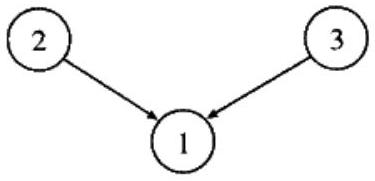
\includegraphics[width=\textwidth]{images/2025_05_15_6a28331d5e7c993ad07ag-030.jpg}
\end{center}

如果一个论证是简单直接的,则完全不需要借助图示去理解它。然而论证往往不是直接的,而图示法能够在平面图上直观地显示论证的结构,因而是非常有用的。${}^{[13]}$ 我们在图中把\textbf{结论}置于\textbf{前提}的下方,而论证的所有前提都在图中的同一行上列出。

与解析法相比,图示法更易于展现论证的前提支持结论的方式。例如在上面这个论证中,前提(2)和(3)都分别独立地支持结论(1):HIV检测呈阳性并不必定是死亡判决。就是说,每个前提自身都为接受结论提供了某种理由,即使没有另一个前提也不影响其为结论所提供的支持。这种\textbf{分立性支持}直观地展现在图示之中。

但是,在有些论证中,只有把前提结合在一起才能达到支持结论的目的。例如:

\begin{quotation}
(1) 我们应该允许安乐死,(2) 如果这样做是最适当地维护所有当事人的利益的话。(3) 而有时候安乐死确实是最适当地维护所有当事人的利益。(4) 因此我们有时候应该允许安乐死。${}^{[14]}$
\end{quotation}

该论证的正确图示将展现出只有当前提之间相结合才能支持结论,即:

\begin{center}
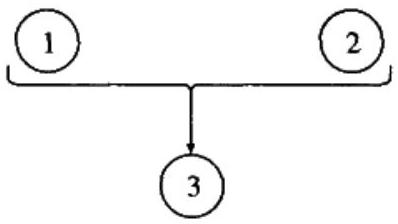
\includegraphics[width=\textwidth]{images/2025_05_15_6a28331d5e7c993ad07ag-031(1).jpg}
\end{center}

此处我们用\textbf{托架线}置于前提之下,是因为在这个例子中两个前提都不能独立地支持结论。如果第一个前提表达的原则是真的,但不存在能够最适当地维护所有当事人的利益的安乐死事例,则结论就根本没有得到支持。而如果的确存在能够最适当地维护所有当事人的利益的安乐死情形,但第一个前提所表述的原则是错误的,则结论仍然没有获得支持。

\subsection{复杂论证的分析}

当论证有更复杂的结构时,图示法就显得特别有用。有时可以很容易地展示出原本很难说清楚的东西。考虑如下论证:

\begin{displayquote}
(1)沙漠高地是天文观测的良好场所。(2)其高度使得它们坐落于大气层之中,使得星光不用穿越整个大气层而到达望远镜。(3)沙漠的干燥度也使之相对较少受云雾干扰。(4)云雾对天空的遮蔽会使许多天文观测归于无用。${}^{[15]}$
\end{displayquote}

命题(1)显然是这个论证的结论,其他三个命题提供对它的支持,但它们支持结论的方式是不一样的。命题(2)自身即可支持沙漠高地是天文观测良好场所的断言,而命题(3)和(4)必须联合起来才能支持这个断言。如下图示可清楚地表明这一点:

\begin{center}
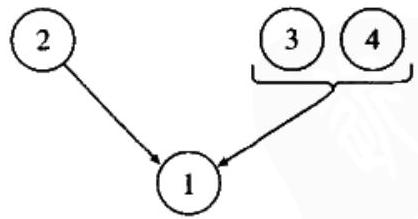
\includegraphics[width=\textwidth]{images/2025_05_15_6a28331d5e7c993ad07ag-031.jpg}
\end{center}

但是某些复杂论证结构的澄清使用解析法更为奏效。例如,当一个论证含有未明确陈述出来的\textbf{隐含前提}时,解析法允许我们直接把隐含前提列出,而图示法则需要既列出隐含前提又要以某种直观形式(如非封闭圆圈)表明它是被附加到原来论说之上的。请考虑如下论证:

\begin{quotation}
只有当我能够做出其他选择时,我对我的行为才负有道德责任。因为一个人若无力避免某行为,就不应被认为对该行为负有道德责任。${}^{[16]}$
\end{quotation}

运用列出隐含前提的解析法,该论证很容易澄清如下:

\begin{enumerate}
  \item 一个人若无力避免某行为,就不应被认为对该行为负有道德责任。
  \item 只有当我能够做出其他选择时,我当下的行为才是我有能力避免的。\\
  所以,只有当我能够做出其他选择时,我对我的行为才负有道德责任。
\end{enumerate}

\subsection{多重复合论证}

当一段话包含两个或更多论证和若干相互关联并不明显的命题时,图示法被证明特别有用。下面是从马克思给恩格斯的一封信中摘录的一段话:

\begin{displayquote}
(1)加速英国的社会革命就是国际工人协会的最重要的目标。(2)而加速这一革命的唯一办法就是使爱尔兰独立。因此,(3)国际的任务就是到处把英国和爱尔兰的冲突提到首要地位,(4)到处都公开站在爱尔兰方面。${}^{[17]}$
\end{displayquote}

一段话中论证的数目通常取决于其中所含结论的数目。这段话中含有两个结论,因而有两个论证。但这两个结论都是从同样的两个前提推得的,如下图示可很好地展示这种结构:

\begin{center}
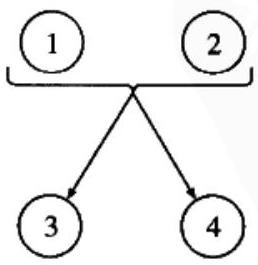
\includegraphics[width=\textwidth]{images/2025_05_15_6a28331d5e7c993ad07ag-032.jpg}
\end{center}

有时,含有两个结论从而有两个论证的一段话,却只含有一个前提。例如:

\begin{quotation}
年纪较大的妇女更难以抵制工作中的性骚扰和离开施暴的丈夫,因为年龄的偏见使她们不容易找到其他保护自己的方式。${}^{[18]}$
\end{quotation}

其中唯一的前提是年纪较大的妇女不容易找到保护自己的方式。该前提支持两个结论:年纪较大的妇女难以抵制工作中的性骚扰,以及她们(对已婚妇女而言)难以离开施暴的丈夫。我们通常用"\textbf{单独论证}"一词指谓只有一个结论的论证,而不管有多少用以支持它的前提。

\subsection{论证中的命题次序}

当一段话中出现两个或更多论证,或一个论证中有两个或更多前提时,就需要弄清各个前提及结论出现的次序。结论可能在最后或最先出现,也可能出现在用以支持它的前提之间,如下例:

\begin{quotation}
穆斯林思想家启示的真正来源是《古兰经》及神圣先知的言论。因而很显然,穆斯林哲学并不是希腊思想的复制品,其所关心的主要是那些来自穆斯林和与穆斯林相关的特定问题。${}^{[19]}$
\end{quotation}

这段话中的结论"穆斯林哲学并不是希腊思想的复制品",出现在论证的第一个前提之后和第二个前提之前。

\subsection{串联式论证}

同一个命题既可在一个论证中做结论,又可在另一个论证中做前提,正如同一个人既可在一个场合做指挥者,又可在另一个场合做被指挥者。托马斯·阿奎那的著作中有一段话可以很好地说明这一点。他说:

\begin{displayquote}
人类的法律是为人类大众制定的,\\
大多数人在德行上是不完美的,\\
因此人类的法律不禁止一切罪恶。${}^{[20]}$
\end{displayquote}

该论证的结论随即被托马斯·阿奎那用做另一个完全不同的论证的前提:

\begin{displayquote}
恶行与善行相反,\\
但人类的法律不禁止一切罪恶,\\
因此人类的法律也不规定一切善行。${}^{[21]}$
\end{displayquote}

\subsection{浓缩论证的分析}

当一系列复杂的论证关系被压缩,对于这样一串浓缩论证的分析,完全解析法会提供很大的帮助。考虑如下论证集合:

\begin{quotation}
因为(1)出现在非洲人种身上的线粒体变种最多,科学家推断,(2)非洲人种的进化史最长,这表明(3)非洲人种可能是现代人类的起源。${}^{[22]}$
\end{quotation}

我们可以把这段论证图示如下:

\begin{center}
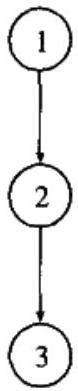
\includegraphics[width=\textwidth]{images/2025_05_15_6a28331d5e7c993ad07ag-034.jpg}
\end{center}

而对这同一串论证的分析,解析法尽管显得不够简洁,但更完整:

\begin{enumerate}
  \item 一个人种身上的线粒体变种越多,其进化史就越长;
  \item 出现在非洲人种身上的线粒体变种最多,\\
  因此非洲人种进化史最长。
\end{enumerate}

\begin{enumerate}
  \item 非洲人种进化史最长,
  \item 现代人类可能起源于进化史最长的人种,\\
  因此现代人类可能起源于非洲人种。
\end{enumerate}

这样的复合论证表明,一个孤立表达的命题既非前提也非结论。在一个论证中,作为假定出现的命题就是前提,被断定为从假定命题推出的命题就是结论。也就是说,"\textbf{前提}"和"\textbf{结论}"都是相对的(relative)术语。

\subsection{交织式论证}

几个论证复合在一起,语言表达上可能不是以串联的方式出现,而是以独特的方式相互交织,这就要求我们对它们做细致的分析。图示法特别适用于这种情况。例如,在约翰·洛克的名篇《政府论》中,下面一段话就有两个论证交织在一起:

\begin{quotation}
立法机构常年运作是不必要的,也是很不方便的;但行政机关常年运作是绝对必要的,因为不是总需要制定新的法律,但总需要执行已制定的法律。
\end{quotation}

上述论证的分支命题可以用数字表示为:(1)立法机构常年运作是不必要的,也是很不方便的,(2)行政机关常年运作是绝对必要的,(3)不是总需要制定新的法律,(4)总需要执行已制定的法律。将这段论证图示如下:

\begin{center}
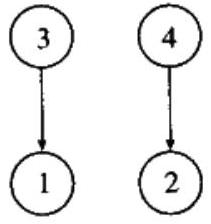
\includegraphics[width=\textwidth]{images/2025_05_15_6a28331d5e7c993ad07ag-035.jpg}
\end{center}

这个图示表明,第二个论证的结论出现在第一个论证的结论和前提之间,第一个论证的前提出现在第二个论证的结论和前提之间。这个图示还表明,两个结论都出现在它们的前提之前。

这个图示同样也展示了支持刑罚威慑理论的古罗马哲学家塞涅卡的两个相关论证的逻辑结构:
\begin{quotation}
(1)惩罚罪行不是因为罪行已经发生,(2)而是为了不发生新的罪行。[因为](3)过去的罪行不能被取消,(4)但是可以预防将来的罪行。
\end{quotation}

在这段话中,"惩罚罪行不是因为罪行已经发生"是其中一个论证的结论,其前提是"过去的罪行不能被取消"。"惩罚罪行是为了不发生新的罪行"是这段话中第二个论证的结论,其前提是"惩罚罪行可以预防将来的罪行"。

\begin{center}
\fbox{\parbox{0.9\textwidth}{
  \centering
  \textbf{论证分析的工具}\\
  解析法和图示法是两种有力的分析工具,运用这两种工具对论证进行分析,\\
  可以更彻底地理解论证前提与结论的关联。
}}
\end{center} 
\section*{1.5 论证的辨识}
\section*{A.结论和前提指示词}
如前所见,出现在论证性话语中的命题的次序不能作为辨识其结论或前提的依据。那么用什么来辨识呢?有一些被叫做"结论指示词"的词或短语有助于这样的辨识,因为它们典型地适合引导出一个论证的结论。下

面所列的就是部分结论指示词 ${ }^{(1)}$ :

\begin{center}
\begin{tabular}{|l|l|}
\hline
therefore(所以) & for these reasons(基于这些理由) \\
\hline
hence(因此) & it follows that(可推得) \\
\hline
thus(因而) & we may infer(我们可推出) \\
\hline
so(故而) & I conclude that(我推断) \\
\hline
accordingly(由此可见) & which shows that(这表明) \\
\hline
in consequence(于是) & which means that(这意味着) \\
\hline
consequently(可得) & which entails that(据此可得) \\
\hline
proves that(据此证明) & which implies that(这蕴涵) \\
\hline
as a result(之所以) & which allows us to infer that(据此我们可以推出) \\
\hline
for this reason(为此缘故) & which points to the conclusion that (据此可得结论) \\
\hline
\end{tabular}
\end{center}

另一些词或短语典型地适合作为论证前提的标志,因而被叫做前提指示词。通常,但非总是,跟在任一前提指示词之后的命题就是某个论证的前提。下面所列的是部分前提指示词:\\
since(因为)\\
because(由于)\\
for(因)\\
as(根据)\\
follows from(从……推出)\\
as shown by(正如……所表明)\\
inasmuch as(缘于)

\section*{B.语境中的论证}
$$
\begin{aligned}
& \text { as indicated by (正如......所示) } \\
& \text { the reason is that (理由是) } \\
& \text { for the reason is that (理由在于) } \\
& \text { may be inferred from (可从.....推出) } \\
& \text { may be derived from (可从......引晴) } \\
& \text { may be deduced from (可从.....得出) } \\
& \text { in view of the fact that (有鉴于) }
\end{aligned}
$$

上面所列的词和短语可以帮助我们认识话语中所含的论证,辨识其前

\footnotetext{(1)下列英汉指示词并非一一对应,在自然语言中识别论证,主要应诉诸语境分析。一一译者注(以下凡脚注均为译者注,不一一标明)
}提或结论,但它们在实际论证中并不一定出现。论证的出现可以由话语的背景或意义来表明。例如,一个女作家用如下陈述对吸烟提出严厉的批评:

是否吸烟是在拥有关于烟草对健康的致命影响的充足信息的情况下做出的有意识的决定。无疑,那些对此做出不明智选择的人,应为其导致健康恶化的后果负责。 ${ }^{[23]}$

这段话中既没有前提指示词,也没有结论指示词,但其中所含的论证是很清楚的。同样,下面一段话中所包含的论证可以从其所含命题本身的意义辨识出来:

\begin{displayquote}
近年来,有关死刑处罚的威慑作用的论证受到人们的反驳。谋杀率最高的二十个州中的十八个州有死刑处罚。谋杀率最高的十七个大城市拥有死刑处罚的司法权。过去十年中,得克萨斯州处死的罪犯比其他任何一个州都多,但得州仍有三个城市的谋杀率列于谋杀率最高的二十五个城市之中。近二十年来,有两个接壤的州的谋杀率基本相当,一个是没有死刑处罚的密歇根州,另一个是有死刑处罚的印第安纳州。 ${ }^{[24]}$
\end{displayquote}

这些语段的论证性功能由它们的语境和它们的意义展现出来。这就好比当我说晚饭时带只龙虾回家,你不会怀疑我是打算吃掉而不是饲养它。

另一个没有结论或前提指示词的论证出现在最近一篇为比例代表制进行辩护的文章中:

单一成员选区(the single-member-district)的选举制度看来有许多严重的彎端。这种制度通常不能代表为数众多的选民的意志,它产生的立法机关不能准确反映公众的看法,它歧视第三党,挫伤选民投票的积极性。[25]

虽然可将这段话看做是首先陈述一个广泛的实际情况,然后用单一成员选 2.3区的选举制度的各种后果去阐明它,但也可以将这段话同样很好地理解为

一个首先陈述其结论,然后从支持这个结论的前提推出这个结论的论证。\\
下面一段最高法院关于公立学校反种族隔离问题的评判中,有一个既无结论指示词又无前提指示词的更复杂一些的论证:

\begin{displayquote}
在学生人数上存在种族不平衡的现象,这不等于表明乡村学校不履行其法律义务。种族平衡本身不是目的。若种族不平衡是由于违背宪法使然,必须予以追究。只要杜绝违法的种族不平衡,乡村学校并没有义务去纠正因人口因素而造成的种族不平衡。 ${ }^{[26]}$
\end{displayquote}

这段话的第一个句子是其所含论证的结论,这个结论可以被解释为"种族不平衡的存在并不表明乡村学校违背了法律"。我们怎么知道它是结论呢?这里语境是决定性的:接在第一个句子后面的几个句子提供了之所以如此的理由。我们看到,在第一个句子中所指谓的"乡村学校"的行为处于争论之中;后面的几个句子表达了几个与乡村学校的行为有关的更一般的命题。话语中所选用的语词也给出了线索,虽然短语"不等于表明"不是结论指示词,但它传达了这样一个暗示,即第一个句子是这段话的逻辑终点。

包含论证的语段经常含有一些既不能作为前提也不能作为结论的附加材料。有时那些提供背景信息的材料能使读者(或听者)理解论证是关于什么内容的。在下面这段话中,论证出现在最后一句中,但如果不抓住它前面句子的内容,这个论证就不可理解:

由于政府削减了对学生的财政援助,许多一流学院和大学都将较大比例的学费收入用做贫困学生的奖学金。正如慈善捐款可免征所得税一样,这部分学费也应亨受税务免征。 ${ }^{[27]}$

严格地讲,这段话中的第一个句子不是论证的一部分,但没有这句话我们就不能理解"这部分"学费是指用做奖学金的那部分学费。据此理解,我们就可以对该论证做如下解释:

1.对贫困者的慈善捐款是免征所得税的。

2.很大一部分学费收人被学校用来作为给贫困学生提供奖学金的慈善捐款。

所以,作为给贫困学生提供奖学金的那部分学费应免征所得税。

可见,上下文中命题之间相互参照,对于理解论证本身是必不可少的。哲学家阿瑟-叔本华在为自杀行为进行(无罪)辩护时所做的一个论证就例示了这种对相互参照的依赖:

\begin{displayquote}
如果罪法禁止自杀,那么在基督教中这并不是一个有根据的论证;而且这个禁令是荒唐的,因为有什么惩罚能让一个连死都不怕的人害怕呢?${ }^{[28]}$
\end{displayquote}

这段话分号前面的句子既非前提也非结论,但是若没有它,我们就不知道在随后出现的论证结论("这个禁令是荒唐的")中的"禁令"乃指谓罪法的自杀禁令。

\section*{C.非陈述形式的前提}
在上一例子中,论证前提以疑问句的形式出现:"有什么惩罚能让一个连死都不怕的人害怕呢?"而正如 1.2 节所述,问题无所断定,不表达命题,那么一个疑问句何以能起到前提的作用呢?这取决于该问句是反诘问句。就是说,当提问者相信问题的答案显然或确定无疑时,可用问句暗示或设定一个前提。在上例中,叔本华认为他的问题的答案明显是"没有",因而,尽管以问句的形式出现,其论证的前提乃是这样一个不言而喻的命题:"没有任何惩罚能够让一个连死都不怕的人害怕。"

前提之一是反诘问句,而问题的答案被设定为明显的,这样的论证是非常普遍的,它们也很有修辞效果。可是这样使用问句是有风险的。例如苏格拉底的如下论证:

美诺啊,如果没有人欲望痛苦,那么就没有人欲望罪恶;因为除了欲望和拥有灾难,还有什么是痛苦的呢?[29]

严格地讲,其中的问句既不真也不假。如果设定为显然或确定无疑的答案

事实上并非如此,那么这个论证就是有缺陷的,而其缺陷正可能被问句掩盖。苏格拉底所假定的痛苦就是欲望和拥有罪恶这个答案是正确的吗?回答并不是显而易见的。

依赖反诘问句的论证,其结论有时是可疑的。人们使用设定有明显答案的问句来做论证的前提,有时就是为了回避直截了当地肯定其前提的责任,而实际上其设定的答案是含糊的甚或是假的。

不过,把真正的反诘问句作为前提使用确是一种很机敏的方法。通过暗示被期望的答案并且引导读者自己引出那个答案,可以增强论证的说服力。考虑下面两个使用反诘问句的例子。《新约全书》中有如下一段话:

\begin{displayquote}
人若说:"我爱神",却恨他的兄弟,就是说谎者:因为不爱他所看见的兄弟,如何能爱他看不见的神呢?[30]
\end{displayquote}

在最近的一篇对安乐死主张进行评论的文章中,有下面一段论证:

\begin{displayquote}
如果安乐死的权利基于自己的决定,那么将其限制到垂死病人就是不合情理的。如果人们有死亡权,那么为什么必须要等到已濒临死亡的时候才能行使这个权利呢?[31]
\end{displayquote}

在上面的两例论证中,两个设问的答案(一个是"不能爱他的兄弟的人也不能爱神",另一个是"人们不必要等到已濒临死亡的时候才能行使死亡权")都被假定是非常明显的。这些答案就是支持预期结论的前提。两个预期的结论分别是:"爱神的人不能恨他的兄弟"和"如果人们有基于自己决定的安乐死的权利,那么就不能将死亡权限制到垂死病人"。

有时论证的结论可以采用祈使句或命令句的形式。在给出劝说我们去采取一个特定的行动的理由后,我们被指导要如此这般地去行动。例如《箴言》(1)中有这样一句话:

\begin{displayquote}
智慧为首,所以要求得智慧。
\end{displayquote}

\footnotetext{(1)Proverbs,见《旧约全书》。
}在《哈姆雷特》中,波洛涅斯对他的儿子雷欧提斯提出如下忠告:

\begin{displayquote}
不要向人告贷,也不要借钱给人;\\
因为债坆放了出去,往往不但丢了本钱,而且还失去了朋友;
\end{displayquote}

向人告货的结果,容易养成因循懒惰的习惯。 ${ }^{[32]}$

因为命令句像一般疑问句一样不能表达命题,所以(严格来讲)命令句不能作为论证的结论。但是为简明计,我们可以把在这些语境中的命令句与命题同样对待,这是很有益处的。在这些语境中听者(或读者)被告知他们应当(should)或应该(ought to)以在命令句中已经说明的方式去行事。那么上面两个论证中的结论可以被解释为:"求得智慧是你应当去做的事情"和"你应该既不借钱给别人也不向别人告贷"。

几乎所有人都会同意,这种断言可以是或真或假的。如果在一个应当去做某事的命令和一个应当做某事的陈述之间有什么区别的话,这种区别恰恰是一个困难的问题,这个问题在这里不必探究。通过忽略这种区别 (如果确有区别的话),我们可以对用命令形式和用陈述形式表达结论的论证做相同的处理。

我们的目的是要更彻底地理解论证。这需要借助于澄清论证的构成命题的作用,尽可能减少依赖语境的因素,从而使论证得以完整地重塑。我们要聚焦于命题本身,探索它们是真的还是假的,它们蕴涵着什么,它们是否被别的命题所蕴涵,在某个论证中它们是否被作为前提或结论。我们要抓住命题的实质,而无论它们的语法形式是什么。

有些论证的完整重塑仅限于语法方面。论证由命题组成,但是表示命题(因此也能表示前提)的话语有时可能采用短语的形式,而不是陈述句形式。下面讨论地外生命可能性的一段话,可以很好地例示这一点:

地外有生命吗?至今仍无定论。但是,有大量的行星;有能够无须近地恒星的能量而生存的生物;有丰富的能产生水的广集无垠的氢和氧的宇宙资源;有行星产生内部热量的各种自然方式;有生命能在海底火山产生并且能足够耐寒地繁殖变体,从而把它们的后代传播到别的世界的可能性;有能够作为星际交流运

載工具的坚固的陨石,凡此种种,生命在宇宙的其他地方演化的思想似乎不再像几年前那样让人感到异想天开。 ${ }^{[33]}$

这段话的结论 一一 地球以外有生命的观念至少比以前更能让人接受一一 得到六个独立前提的支持,每个前提都让人注意到近来发现的事实或可能性,每个前提都表达支持存在地外生命的理由。当这些前提被重新解释为陈述句时,如:(1)宇宙间有大量的其他行星存在;(2)有许多生命能够不依靠近地恒星的能量而生存;等等,这段话中所表达的论证也就变得明显起来。

\section*{D.未明确陈述的命题}
当论证中有一个或更多构成命题未明确陈述出来但又假设能为人理解时,论证的分析可能变得更复杂。在2000年4月美国最高法院对著名的米兰达规则进行辩论的会议上,就有这样的例子。(米兰达规则规定:除非被监禁的嫌疑人在审问开始前被告知有权保持沉默并有权请律师,否则法庭不得采信嫌疑人在接受警察审问时所做的认罪供述。)米兰达规则的辩护人论证如下:

如果米兰达规则被推翻,将不再强制性地要求警察预先给予 (有权保持沉默等的)告知;如果不强制性地要求警察预先给予告知,他们将不会预先告知。但是因为警察的审问是在公共视域以外进行,仅当总是给予米兰达告知,这些审问的完善性才能得到维护。 ${ }^{[34]}$

此处辩护人论证的结论一一必须始终给予预先告知,最高法院不应当推翻米兰达规则——不必陈述出来。

在另一个完全不同的语境中,著名小说家安奈斯•林这样描写她的一个小说人物:"梦想家拒绝平凡,杰伊向往平凡。"${ }^{[35]}$ 我们可以推断出作者试图传达的内容——"杰伊不是梦想家"——即使没有陈述出来。

由于论证者假设的论证前提之一是人所共知的或他认为很容易就被人承认的,就可能不陈述出来。在莎士比亚的《裘利斯•恺撒》中,当马克-安东尼正在做关于恺撒的野心的著名演说时,一个市民听众评论

恺撒说:

这是一个论证,但省略了一部分前提,它明显依赖一个合理的但未陈述出来的前提:"不愿接受王冠的人一定没有野心"。日常语言中的三段论论证经常依赖某个未陈述出来的命题。这样的论证叫做省略三段论。 ${ }^{[37]}$

究竟如何揭示说话人所依赖的(省略)命题,有时并不是很明显的,尽管一旦将其表示出来就很容易被接受。在最近的一部有关美国奴隶制的历史争论以及在那个争论中道德论证所起的作用的著作中,作者写道:

\begin{displayquote}
如果不相信道德论证能产生任何影响,那就是不相信共和政体的政府。 ${ }^{[38]}$
\end{displayquote}

在这个省略式中,未陈述出来的前提是这样一个断定:"相信共和政体的政府要求人们相信道德论证能产生一定的影响"——一个我们多数人都会认可的断言。

此外,省略三段论所依赖的未陈述出来的命题有可能并不显然,而是可质疑的;不把它明确陈述出来,可能正是为了使之避受责难。例如,使用胚胎干细胞进行医学研究广受质疑,一位美国参议员用下面的省略三段论抨击允许政府筹措资金进行这项研究的法案:

\begin{displayquote}
这项研究(包含对胚胎干细胞的使用)是非法的,这是因为:故意杀死人类胚胎是这项研究的基本组成部分。 ${ }^{[39]}$
\end{displayquote}

该论证陈述出来的前提是真的:如果胚胎不被杀死,这项研究是不可能进行的。但是,这项研究是非法的这个结论却依赖其未表述出来的命题:杀死人类胚胎是非法的,而这正是一个处于激烈争论中的论断。

省略三段论极其依赖语境,也经常依赖于听话者关于某个表述出来的命题为假的知识。当论证的目的是强调某个命题的虚假性时,说话人常常

构造这样一个假言命题:以该命题作前件("如果"部分),以一个普遍认为为假的命题作后件("那么"部分)。例如, 18 世纪著名的巴伐利亚风琴制造商之一约瑟夫-瑞普就他的管风琴说过一句广为人知的豪言:"如果在欧洲能发现更好的管风琴,那么我的名字就叫杰克。"因为所有人都会明白,在一个真的假言陈述中,如果后件是假的,前件就不能是真的。对这个假言命题的肯定,实际上就是一个省略式论证,即旨在嘲讽其前件命题:在欧洲能发现更好的管风琴。论证的结论(在欧洲不能发现更好的管风琴)和另一前提(我的名字不叫杰克)都没有表述出来。 ${ }^{[40]}$ 
\section*{1.6 论证和说明}
许多语段,无论是书面语还是口语,看起来好像是论证,实际上不是论证而是说明。即使有某些前提或结论指示词出现,例如"因为"、"由于"、"因此"等,也不能解决问题,因为这些语词既可用在论证中也可用在说明中。我们必须知道在这些语段中作者的意图。[41]

请比较下面两段话:

1.为你自己积损财宝在天上,天上没有虫子咬,不能锈坏,也没有淢挖窟窟来偷,因为你的财宝在哪里,你的心也在哪里。

2.所以它(那座塔)名叫巴别,因为耶和华在那里变乱天下人的言语。\\
——《创世记》11: 19

第一段话是一个清楚的论证,它的结论,即一个人必须积攒财宝在天上,由前提(这里用"因为"来标明)一个人的财宝积攒在哪里,他的心也在哪里来支持。但是第二段不是论证,尽管它非常恰当地使用了"所以"一词。它说明了这座塔(其建造过程在《创世记》中有详细的叙述)为什么叫巴别。它告诉我们,因为之前人类在那里使用的是同一种语言,现在被许多语言变乱了,所以给塔起了这个名字。 ${}^{[42]}$ 这段话假设读者知道那座塔有这个名字,意图是说明为什么给塔起了这个名字。短语"所以它名叫巴别"不是结论而是完成了对这个名字的说明。句子"因为耶和华在那里变乱天下人的言语"不是前提,它不能作为相信巴别是那座塔名字的原因,因为巴别是那座塔的名字的事实是这段话所要为之做说明的读者所知道的。在这个语境中"因为"指示的是接下来要说明将巴别这个名字给予那座塔的原因。

上面两段话说明一个事实,表面上相似的语段可能具有完全不同的功能。任何一个特定的语段究竟是论证还是说明,这取决于那个语段所服务的目的。如果我们的目的是要确立某个命题 Q 的真,为此我们提出某个证据 P 来支持 Q ,我们可以恰当地说" Q 因为 P "。也就是说我们为 Q 建立一个论证, P 是我们的前提。但是假设 Q 是已知为真的。在这种情况下我们不必提出任何理由来支持它的真一一但是我们可以希望对它为什么是真的给出一个说明。这样我们也可以说" Q 因为 P "——但在这种情况下,我们不是为 Q 建立一个论证,而是给出一个对 Q 的说明。

在回答关于类星体(在我们的星系以外很远地方的一类天体)的外观颜色的问题时,一位科学家写道:

\begin{displayquote}
最远的类星体看上去像强烈的红外辐射光点。这是因为太空散布着吸收蓝光的氢微粒 (大约每立方米两个微粒), 如果你从可见的白光里过滤掉蓝光, 那么剩下的就是红光。在其到达地球的数十䎲光年的旅程中, 类星体光被大气中的氢微粒吸去了全部的蓝光, 留下的只有红光。[43]
\end{displayquote}

这段话不是论证,它不是试图要让读者确信类星体具有像它们所显示的外观颜色,而是说明它们具有这个外观颜色的原因。

同样,在讨论不列颠对非洲早期发展的影响时,一个历史学家写道:

\begin{abstract}
塞拉利昂在1808年成为英国直辖殖民地不是因为它的繁荣,而是因为它的萧条。由于战争和商业不景气的负担,塞拉利昂的私营公司不能支付它们的费用,而刚刚废除了贩卖奴隶制度的英国政府感到有必要接管它。 ${ }^{[44]}$
\end{abstract}

这里没有对塞拉利昂在1808年成为英国直辖殖民地这个结论进行论证。塞拉利昂在那时确实成了英国直辖殖民地。但这是为什么呢?乃是由于在本例和前例中,"因为"很明显是说明的标志,而不是论证的标志。

我们怎么才能断定一个语段的目的是打算说明还是打算说服人呢?通常我们可以根据" Q 因为 P "这个形式提问,对于作者来说 Q 的身份是什么,以此来做出区分。若 Q 是一个其真实性需要建立的命题,那么"因为 P "可能给出了支持其为真的前提,这样"Q 因为 P "就是一个论证。若 Q 是一个已知其为真,或至少在这个语境中其真是没有疑问的命题,那么"因为 P "就可能是对为什么 Q 成为真命题的阐释,这样" Q 因为 P "就是一个说明。

在一个说明中,人们必须把什么是被说明的东西,与什么是用来说明的东西区别开来。在上面《创世记》所做出的说明中,被说明的内容是为何那座塔具有名字巴别,说明的内容是在那里耶和华变乱天下人的言语。在上面刚给出的历史学的例子中,被说明的内容是塞拉利昂成为不列颠直辖殖民地,说明的内容是塞拉利昂公司的无支付能力和不列颠政府就此做出的回应。

有时被称做说明的东西实际上可能是论证,反之亦然。不久以前,《纽约时报》由于对待男女性别的不平等做法而受到一个读者的批评,因为它对一个著名女演员的不断增长的体重加以评论,但对在同一篇报道中提到的一个杰出商人的不断增长的体重却没有评论。后有另一个读者对此做出回应:

E.R.福克斯的抱怨——你特别提到凯瑟琳•丹尼芙"也许不像她以前那么苗条",但你没有提及唐纳德•杜鲁普不断增加

的腰围——很容易说明。杜鲁普先生从未裸体出现在电影中以使他的体形成为人们感兴趣的事情。 ${ }^{[45]}$

这不是一个真正的说明,而是一个论证。它有两个前提,第一,裸体外表出现在电影中使一个人的外表成为人们感兴趣的事情,第二,杜鲁普先生从未以裸体外表出现在电影中,而丹尼芙女士有过。因此,报纸对如此出现在电影中的名人的体形加以评论,而忽略未如此出现在电影中的名人的体形,这种做法就是合乎情理的(这个读者的主张),据此抱怨对待男女性别不平等就是不应当的。

为了区别说明和论证,我们必须对语境有一定的敏感性。总会有一些语段,其目的难以确定。一个其目的难以确定的语段可能需要给予两种同样有道理的"解读"一一用一种方法去解读,被当做论证;用另一种方法解读,就是说明。 
\section{演绎和有效性}

\begin{quotation}
\textit{演绎论证是逻辑学的核心研究对象,了解演绎论证的本质及其有效性标准是进行逻辑分析的基础。}
\end{quotation}

每一个论证都是断言其前提为结论的真提供理由。实际上这种断言正是论证的标志。但是论证有两大不同种类:\textbf{演绎论证}和\textbf{归纳论证}。这两类论证在其前提支持结论的方式上有着根本的不同。本节我们对演绎论证作一个简要的阐释。

任一演绎论证均断言其前提\textbf{决定性地}(conclusively)支持结论。相反,归纳论证均没有这种断言。在对一个语段的解释中,如果我们判定它做出了这样的断言,我们就将其视为演绎论证;如果我们判定它没有做出这样的断言,我们就将其视为归纳论证。因为每个论证都会对决定性支持结论或者做出断言,或者不做出断定,所以每个论证或者是演绎的,或者是归纳的。

当一个论证断言它的前提(如果是真的)为它的结论的真提供了无可辩驳的理由时,这个断言或者是正确的或者是不正确的。如果是正确的,这个论证就是\textbf{有效的}。如果不是正确的(也就是说,即使前提是真的,也不能无可辩驳地确立其结论的真),那么这个论证就是\textbf{无效的}。

因此,对于逻辑学家而言,有效性这个术语仅仅对演绎论证才是适当的。说一个演绎论证是有效的,就是说如果其前提是真的,其结论为假就是不可能的。这样我们可把\textbf{有效性}定义如下:一个演绎论证是有效的,即如果其前提是真的,则其结论必定是真的。

每个演绎论证都要求其前提为其结论的真提供担保,但并非所有演绎论证都能做到这个要求。不能做到这个要求的演绎论证就是无效的。

因为每个演绎论证就其目标的实现而言或者是成功的或者是不成功的,所以每个演绎论证或者是有效的或者是无效的。这一点非常重要:如果一个演绎论证不是有效的,它一定是无效的;如果它不是无效的,它一定是有效的。

演绎逻辑的中心任务(将在本书第二部分详细讨论)就是对有效论证和无效论证做出区分。为此,古往今来逻辑学家们发明了许多非常有效的方法。但用来判定论证有效性的传统方法不同于大多数现代逻辑学家使用的方法。前者被叫做\textbf{古典逻辑},发端于亚里士多德的分析工作,本书的第5、6、7章将对此加以阐释。\textbf{现代符号逻辑}的方法将在本书的第8、9、10章详加介绍。尽管两个流派的逻辑学家们在方法上和对某些论证的具体阐释上不尽一致,但他们都同意演绎逻辑的主要任务是开发一种能使我们区分有效论证与无效论证的工具。

\begin{center}
\fbox{\parbox{0.9\textwidth}{
  \centering
  \textbf{演绎论证的本质与有效性}\\
  演绎论证断言其前提决定性地支持结论,当且仅当前提为真时结论必然为真,\\
  这种论证才被视为有效;判定论证有效性是演绎逻辑的核心任务。
}}
\end{center} 
\section{归纳和或然性}

\begin{quotation}
\textit{归纳论证是科学研究和日常推理的基础,它与演绎论证有着根本的区别,理解其依赖的或然性原则是进行有效分析的关键。}
\end{quotation}

\textbf{归纳论证}不要求它们的前提必然地支持结论,纵然其前提是真的。它提出一个较弱的但仍然是很重要的要求:其前提\textbf{或然性地}支持结论。或然性总是必然性的缺乏,因而上述关于有效性和无效性的讨论并不适用于归纳论证:归纳论证既不是有效的也不是无效的。$^{[46]}$ 当然,我们仍然可以对它们进行评估。实际上,对归纳论证进行评估是任何领域的科学家最主要的任务之一。归纳论证的前提为它的结论提供某种支持,前提授予结论的或然性程度越高,论证的价值也就越大。一般情况下,我们可以说归纳论证"较好"或"较差","较弱"或"较强",等等。但是,甚至在所有前提都是真的并且对其结论提供了非常强的支持的情况下,归纳论证的结论也不是必然得出的。归纳理论,归纳推理的技巧,评估归纳论证的方法,以及量化和推测或然概率的方法等将在本书第三部分详加介绍。

\subsection{归纳与演绎的根本区别}

归纳论证和演绎论证之间的区别是根本性的。因为归纳论证的前提对其结论的支持都具有某种程度的或然性,附加的信息就有可能强化或弱化这种或然性。新发现的事实可以使我们改变对或然性的估价,可能导致我们对归纳论证的判定比我们原想的更好(或更差)。在归纳论证的领域——即使当结论被认为具有很高可能性的情况下——永远不会穷尽所有的证据。正是这种发现与我们以前所相信的证据相冲突的新材料的可能性,使得我们不能断定任何归纳论证的结论具有绝对的确定性。

相反,\textbf{演绎论证}却不能越来越好或越来越差。它们在显示前提和结论之间的令人信服的关系上要么成功要么失败。这个对比揭示了演绎和归纳之间的根本差异。如果一个演绎论证是有效的,就没有附加的前提可以增强这个论证的有效性。例如,如果凡人皆终有一死,并且如果苏格拉底是人,我们就可以毫无保留地得出结论,苏格拉底终有一死——即苏格拉底终有一死的结论总能从那两个前提推论出来,而不管世界上别的什么可能是真的,也不管别的什么信息被发现或增加到该论证的前提当中。比如我们后来又知道苏格拉底难看,或天使永生,或奶牛产奶,但这些发现和别的发现都不能对原来的论证产生任何影响。

就每一个有效的演绎论证来说,不管附加前提的性质如何,从其前提必然推出的结论同样也能必然地从任何扩大的前提集推论出来。如果一个论证是有效的,世界上就没有什么东西能使它更有效;如果一个结论是从某个前提集有效推出的,就没有什么东西可以增加到这个前提集当中使得该结论的推出变得更严格、更合乎逻辑或更有效。

\subsection{归纳论证示例及其特征}

但归纳论证并不是这样,归纳论证所断言的前提和结论之间的关系远非如此严格,与演绎论证有本质上的不同。考虑下面这个归纳论证:

\begin{displayquote}
大部分公司法律顾问是保守主义者,\\
安吉拉•帕尔默瑞是一个公司法律顾问,所以安吉拉•帕尔默瑞很可能是保守主义者。
\end{displayquote}

这是一个非常好的归纳论证,它的第一个前提是真的,如果它的第二个前提也是真的,则其结论很可能就是真的而不是假的。但是在这种场合(与有关苏格拉底的必死性的论证形成鲜明对照),若增加某个新前提到原来的论证之中,就可能会弱化或强化(依据新前提的内容)原来的论证。假设我们还知道:

安吉拉•帕尔默瑞是美国公民自由权协会(ACLU)的一名官员。

又假设在原论证中增加一个(真)前提:

美国公民自由权协会的大部分官员不是保守主义者。

那么那个结论(安吉拉•帕尔默瑞是一个保守主义者)不再看起来非常可能,原来的归纳论证由于这个关于安吉拉•帕尔默瑞的附加信息的出现而被大大弱化。而如果上述前提被改造成全称命题:

没有美国公民自由权协会的官员是保守主义者。

那么就会有效地从被断定的前提集演绎地推出与原来结论相反的结论。

另一方面,假设我们通过增加下面的附加前提来扩大原来的前提集:

安吉拉•帕尔默瑞长期是国家步枪协会(NRA)的一名官员。

和

安吉拉•帕尔默瑞被任命为保守的《国家评论》报的特约撰稿人。

那么通过这个扩大了的前提集,原来的结论就得到了比原来的前提集更大的支持。

\subsection{两类论证的本质特征}

总之,归纳和演绎的区别依赖于两类论证对前提和结论之间的关系所作断言的性质。我们可以将两类论证的特征表示如下:

\textbf{演绎论证}是一种其结论被断言为从其前提\textbf{绝对必然地}推出的论证,这种必然性不是一个程度问题,不以任何其他事物情况为转移。反之,\textbf{归纳论证}是一种其结论被断言为仅仅\textbf{或然性地}从其前提推出的论证,这种或然性是一个程度问题,其程度受可能出现的其他事物情况的影响。

归纳论证并不总是明确表明其结论仅仅是在某种或然程度上推出来的。另一方面,在一个论证中出现"或然性"一词也并不一定表明该论证就是归纳的。这是因为有一些严格的演绎论证是关于或然性本身的。$^{[47]}$ 在这种论证中,事件之间的确定联系的或然性是从另外的事件的或然性演绎推出的,这个问题将在第14章讨论。

\begin{center}
\fbox{\parbox{0.9\textwidth}{
  \centering
  \textbf{归纳与演绎论证的对比}\\
  演绎论证的结论必然地从前提推出,新信息不能影响其有效性;\\
  归纳论证的结论仅或然地从前提推出,其强度可能随新证据的增加而增强或减弱。
}}
\end{center}
\section{有效性和真实性}

\begin{quotation}
\textit{理解有效性与真实性的区别是逻辑分析的基础,这两个概念分别适用于论证和命题,正确把握它们的关系对评估推理至关重要。}
\end{quotation}

如前表明,一个成功的演绎论证是有效的。\textbf{有效性}指谓命题之间的一种关联——作为演绎论证前提的命题集和作为该论证的结论的一个命题之间的关联。如果后者是逻辑必然地从前者推出的,我们就说该论证是有效的。因为归纳论证永远达不到逻辑必然,有效性永远不适用它们。有效性也永远不能适用于任何独立的单一命题本身,因为在任何一个命题内部都不可能找到这种必需的关联。

另一方面,\textbf{真和假}都是单个命题的特征。在论证中作为前提的单个陈述可能是真的或假的,作为其结论的陈述可能是真的或假的。结论可以被有效地推论出来,但是说任何结论或任何单一的前提本身是有效的或无效的,都是无意义的。

\subsection{真实性与命题}

真,是其断言与实际情形相一致的命题的属性。当我断定苏必利尔湖是北美洲五大湖中最大的湖时,我的断言确与实际情形相一致,从而就是真的。如果我说北美洲五大湖中最大的是密歇根湖,我的断定就与实在世界不一致,因此就是假的。这个对比是重要的:\textbf{真和假是单一的命题或陈述的属性;有效性和无效性是论证的属性}。

正如有效性这个概念不适用于单一的命题,真这个概念也不能应用于论证。一个论证中的几个命题,其中的一些(或全部)可以是真的,并且其中的一些(或全部)可以是假的。但是论证作为一个整体,既不"真"也不"假"。关于世界的陈述的命题可以是真的或假的,由从一个命题集到其他命题的推论构成的演绎论证可以是有效的或无效的。

真(或假)命题与有效(或无效)论证之间的关系处于演绎逻辑的中心地位。本书第二部分主要致力于分析它们之间的这些复杂关系。不过,在这里对有效性和真实性之间的关系作一初步的讨论也是适宜的。

\subsection{有效性与真假前提}

即使一个论证的一个或几个前提不是真的,这个论证也可能是有效的,我们的讨论就从强调这一点入手。每个论证都对其前提和从这些前提推导出的结论之间的关联做出断言;即使这些前提被证明为假或其真实性受到质疑,这种关联也是成立的。1858年亚伯拉罕•林肯在与斯蒂芬•道格拉斯的一场争论中有力地运用了这一点。林肯对强迫逃跑到北方各州的奴隶返回他们在南方的主人家里的德雷德-司各特决议进行抨击说:

\begin{quotation}
考虑到人们的论辩能力,我把德雷德•司各特决议用三段论形式表述如下,可以看出这个论证中是否有错误:

任何一个州的任何法规和法律都不能破坏美国宪法中所清楚、明确地规定的权利。

美国宪法中清楚、明确地规定了对奴隶的财产权。

所以任何一个州的任何法规和法律都不能破坏对奴隶的财产权。
\end{quotation}

我相信这个论证挑不出什么毛病。假设其前提都是真的,从这些前提必然会推出上述结论,这个结论我完全有能力理解。但我认为其中确有一个毛病,但这毛病不在于推理,事实上这个毛病是有一个前提是错误的。我相信对奴隶的财产权并不是宪法中清楚明确地规定的,而道格拉斯法官认为是的。我相信最高法院和那个决议(德雷德•司各特决议)的拥护者要想在宪法中查找到对奴隶的财产权的清楚明确的规定将会是徒劳的。所以我说,我认为事实上上述推理前提之一不是真的。$^{[48]}$

在他加以概括并予以抨击的那个论证中,林肯发现第二个前提——美国宪法中规定了对奴隶的财产权——明显是假的。他指出,那个论证中的推理不是错误的,然而它的结论却没有得到证明。林肯的逻辑观点是正确的:甚至在一个论证的结论和其一个或几个前提都为假时,这个论证也可以是有效的。我们再一次强调,一个论证的有效性仅仅依赖于其前提与结论之间的关联。

\subsection{真实性和有效性的组合关系}

在有效的和无效的论证中,真的和假的前提与结论之间有许多可能的组合。考虑下列作为例示的论证,每一个论证之前都有一个对其前提与结论的真假组合的简短陈述。通过这些例证,我们可以完整地列出有关真实性和有效性之间的关系的重要原则。

I.有些有效的论证只包含真命题——真前提和真结论。

\begin{quotation}
所有哺乳动物都有肺,所有鲸鱼都是哺乳动物,所以所有鲸鱼都有肺。
\end{quotation}

II.有些有效的论证只包含假命题:

\begin{quotation}
所有四条腿的生物都有翅膀,所有蜘蛛都是四条腿的,所以所有蜘蛛都有翅膀。
\end{quotation}

这个论证是有效的,因为如果其前提是真的,其结论也一定是真的——即使我们知道这个论证的前提和结论实际上都是假的。

III.有些无效的论证只包含真命题——它们的所有前提都是真的,它们的结论也是真的。

\begin{quotation}
如果我拥有福特•诺克斯的所有财富,那么我将是富有的,我不拥有福特•诺克斯的所有财富,所以我不是富有的。
\end{quotation}

IV.一些无效的论证只包含真前提,但有一个假结论。这可以用一个与前面的论证(III)在形式上完全相同,仅仅换一个假结论的论证来说明:

\begin{quotation}
如果比尔•盖茨拥有福特•诺克斯的所有财富,那么比尔•盖茨将是富有的,

比尔•盖茨不拥有福特•诺克斯的所有财富,

所以比尔•盖茨不是富有的。
\end{quotation}

这个论证的前提是真的,但结论是假的。这样的论证不会是有效的,因为有效的论证不可能前提真而结论假。

V.有些有效的论证有假前提和真结论:

\begin{quotation}
所有鱼是哺乳动物,

所有鲸是鱼,

所以所有鲸是哺乳动物。
\end{quotation}

如我们所知,这个论证的结论是真的;而这个结论可以从两个都不符合实际的假前提有效地推论出来。

VI.一些无效的论证也有假前提和真结论:

\begin{quotation}
所有哺乳动物都有翅膀,

所有鲸都有翅膀,

所以所有鲸都是哺乳动物。
\end{quotation}

从例V和例VI可以看出,很显然我们不能从一个论证有假前提和真结论推断该论证是有效的还是无效的。

VII.当然,有些无效的论证包含的都是假命题——假前提和假结论:

\begin{quotation}
所有哺乳动物都有翅膀,

所有鲸都有翅膀,

所以所有哺乳动物都是鲸。
\end{quotation}

这七个例子清楚地表明,有结论为假的有效论证(例II),也有结论为真的无效论证(例III和例VI)。因此很显然,一个论证的结论的真或假自身并不决定那个论证的有效性或无效性。此外,一个论证有效不能保证其结论的真实性(例II)。

下面两个表格(涉及前面的七个例子)清楚地表明了论证前提与结论可能组合的种类。第一个表格表明,无效论证可以具有真的和假的前提与结论的每一种可能组合:

\begin{center}
\begin{tabular}{|c|c|c|}
\hline
\multicolumn{3}{|c|}{无效的论证} \\
\hline
 & 真结论 & 假结论 \\
\hline
真前提 & 例III & 例IV \\
\hline
假前提 & 例VI & 例VII \\
\hline
\end{tabular}
\end{center}

第二个表格表明,有效论证只能具有真的和假的前提与结论的可能组合的三种情况:

\begin{center}
\begin{tabular}{|c|c|c|}
\hline
\multicolumn{3}{|c|}{有效的论证} \\
\hline
 & 真结论 & 假结论 \\
\hline
真前提 & 例I & \multicolumn{1}{|c|}{} \\
\hline
假前提 & 例V & 例II \\
\hline
\end{tabular}
\end{center}

\subsection{有效论证与可靠性}

第二个表格的那个空格位置显示了非常重要的一点:如果一个论证是有效的并且其前提都是真的,我们就可以断定其结论也是真的。换句话说:\textbf{如果一个论证是有效的并且其结论是假的,那么其前提不会都是真的}——肯定有至少一个假前提。

有效加上真前提等于\textbf{可靠}。一个可靠的论证必定有真结论。只有可靠的论证才能确立其结论的真实性。如果一个演绎论证不是可靠的——也就是说,如果这个论证不是有效的,或者如果其前提并非都是真的——即使其结论事实上是真的,其结论的真实性在论证中也得不到确立。

检验前提的真实性或虚假性是一般科学的任务,因为前提完全可以涉及任意的题材。逻辑学家的主要兴趣不在于命题的真实性或虚假性,而在于命题之间的\textbf{逻辑关系}。所谓命题之间的"逻辑"关系,指的是决定其所出现于其中的论证的(形式)正确性或不正确性的命题之间的那些关系。决定论证的(形式)正确性或不正确性的任务正好落在逻辑学的领域内。逻辑学家甚至对前提可能为假的论证的(形式)正确性感兴趣。

为什么不把我们的研究限制在真前提论证的范围内,而忽略所有其他论证呢?这是因为,那些前提的真实性不为人们所知的论证的(形式)正确性,有可能是非常重要的。例如,在科学研究中,我们通过推断出可检验的结果来检验理论——但是我们不能预先知道哪个理论是真的。又如,在日常生活中,我们经常必须在可供选择的两个行动方向之间做出选择,推断每个行动方向的后果。为了避免选错,我们必须对可供选择的两个选项做出正确的推理,将每个选择作为一个前提。如果我们仅仅对前提为真的论证感兴趣,那么只有当我们知道了可供选择的两个前提哪个是真的,我们才能知道去找出它的结论集。但是如果我们知道可供选择的两个前提哪个是真的,我们就完全不必对它做出推理,因为我们推理的目的就是帮助我们对应该断定哪一个可供选择的前提为真做出决定。所以,如果把我们的注意力限制在前提已知为真的论证上,将使我们的目标不能实现。

确定演绎论证的有效性或无效性的一些富有成效的方法将在本书第二部分介绍并阐释。

\begin{center}
\fbox{\parbox{0.9\textwidth}{
  \centering
  \textbf{有效性与真实性的关系}\\
  有效性适用于论证,描述前提与结论之间的逻辑关系;\\
  真实性适用于命题,描述命题与世界事实的一致性;\\
  只有既有效又具有真前提的论证(可靠论证)才能确立结论的真实性。
}}
\end{center} 
\section*{1.10 复杂的论证性语段}
实际论证有可能是非常复杂的。有些语段中的论证是由几个论证多重复合而成,语段中有些命题只作为前提,有些命题既作为前提又作为分结论,这样的语段分析起来就比较困难。图示法的技术就非常有助于分析这种语段,但并不存在一种建构图示以精确地描述这样的语段的机械方法。此外,因为对这种语段可以作几种合理的解释,因此也可以合理地考虑几种不同图示来展现其逻辑结构。

为了清楚地分析复杂语段,我们必须努力理解作者推理的流程,辨识

语段中每个成分的作用。下面的例子(为便于分析,其中的分支命题用数字标出)显示了我们阐明前提和结论之间的联系的方法。一旦辨识出一段话语中所含的论证以及论证之间的关系,我们就能够对这些论证的结论是否真正是从被断定的前提中推论出来的做出判定。

在下列论证集合中,语段最后的结论就是第一个陈述,这不奇怪。有四个前提直接支持这个结论,其中的两个前提又是分结论,逐次得到语段中所断言的其他前提不同方式的支持:

\begin{displayquote}
(1)看来, 用动物实验进行科学研究的做法并不是不必要的或靠不住的; (2)在使用脊椎动物进行实验之前, 实验的草案必须经过包括一名兽医和一名公众代表在内的公共机构委员会进行的再审查, 并且(3)在研究期间, 动物的医疗和卫生情况得到定期监测。(4)研究者需要健康的动物进行科学研究和医学研究, 因为(5)不健康的动物可能导致错误的研究结果。这激励(6)科学家确保他们使用的任何动物健康并且营养良好。此外, (7)用动物进行研究是昂贵的, 因为(8)料学研究的资金受到限制, (9)只有高质量的研究才能通过有力的竞争获得对研究的支持。[49]
\end{displayquote}

下面的图示展示了这段话的逻辑结构。检查这样的图示,从那些在图中最高处因而在逻辑串联中也是最早的地方开始,通过用数字替换表达出来的命题,有助于对它们进行"解读"。也就是说,人们能够从推理的几条路线的每一条路径推出最后的结论。\\
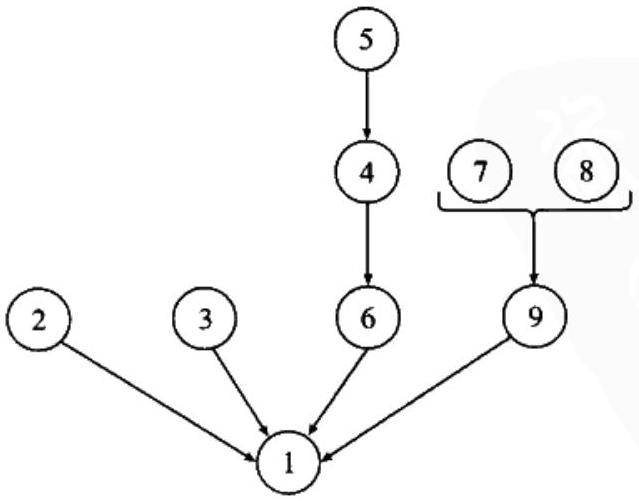
\includegraphics[max width=\textwidth, center]{2025_05_15_6a28331d5e7c993ad07ag-072}

在一个论证中,单个的命题有时以不同语词表达的语句形式重复出现,有时是为了强调,有时又被省略。这种强调使得分析工作复杂化。图示法有助于分析,因为我们可以用相同的数字表示相同命题的不同表述。下面一段话由三个清楚的论证构成,有些命题重复多次出现:

\begin{displayquote}
(1)宇宙大爆炸理论正在瓦解……(2)根据正统知识, 宇宙起源于大爆炸一 -200 亿年前的一次巨大的、非常匀称的爆炸。问题是(3)天文学家通过进一步观测证实: 现存的巨大星系团因为体积太大, 完全不可能在仅仅 200 亿年时间中形成……通过人造卫星所收集的新材料的研究, 以及较早前的地面测量表明(4)星系聚集成绵延数十亿光年的巨大带状, 并且(5)星系之间有亿方光年的距离。因为(6)据观测, 星系移动的速度远不及光速, 数学家证明(7)聚集成这么大的物质团必须要经过至少 1000 亿年时间一是假设的大爆炸时间的五倍……(3)像那么大的一种结构现在看来不可能在 200亿年时间中形成……(2)大爆炸理论认为, 物质均匀地散布在宇宙中。而与这种理想理论相反, (3)这么巨大的星丛无法这么快地形成。[50]
\end{displayquote}

在这段话中,报告观察证据的前提(4)、(5)、(6)为(7)即自大爆炸起必须经过非常长的时间提供理由。这被用来支持分结论(以三种略有不同的方式表述)即(3)像那么大的一种结构现在看来因为太大,不可能在那段时间中形成。从 (3)这个结论,结合(2)即对大爆炸理论假设的原始对称和扩散的简短陈述(以两种略有不同的方式表述),我们可以推论出这段话最后的结论(1):大爆炸理论正在瓦解——这段话开头的命题。下面的图示展示了这段话的逻辑关系集:\\
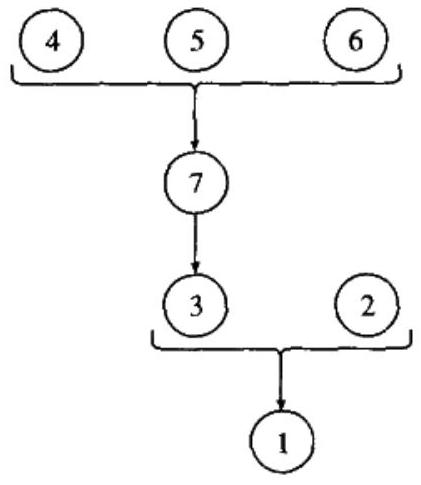
\includegraphics[max width=\textwidth, center]{2025_05_15_6a28331d5e7c993ad07ag-073}

分析论证,必须注意前提可能以浓缩形式出现的情形,有时前提只以一个名词性短语来表示。在下面的论证中短语"在大气中的散射"作为前提(4),可以重塑为"太阳的能量散射在大气中"。浓缩与重复使得对下列论证的分析更加困难:

\begin{displayquote}
(1)太阳能汽车只是一种试验性的装置, 其他什么都不是。(2)太阳的能量太弱以至于不能发动甚至是日常使用的迷你汽车。(3)进入大气层的太阳能量大约为每平方码 1 千瓦。因为(4)在大气中的散射, 又因为(5)地球上的任何地方一天中平均只有半天时间受到阳光的照射, (6)每天接收的太阳功率平均为 $1 / 6$ 千瓦时到 4千瓦时 $\cdots \cdots$ 对通常规格的汽车的检测表明, (7)若使一辆电车勉强能够工作, 其电池组需要 300 千瓦时的能量。因此, (8)充满汽车电池必须有 40 平方码的原电池, 大约是一辆拖拉机的拖车顶部的尺寸。(1)除了用于昂贵的试验汽车外, 太阳能没有指望成为任何汽车的动力, 太阳能汽车不是一项待开发的技术。这就是结论。[51]
\end{displayquote}

这段话中的第一个命题,即"太阳能汽车只是一种试验性的装置,其他什么都不是"的断定,是最后的结论。语段的最后以更加复杂的形式重复了这一结论。这段话的图示为:\\
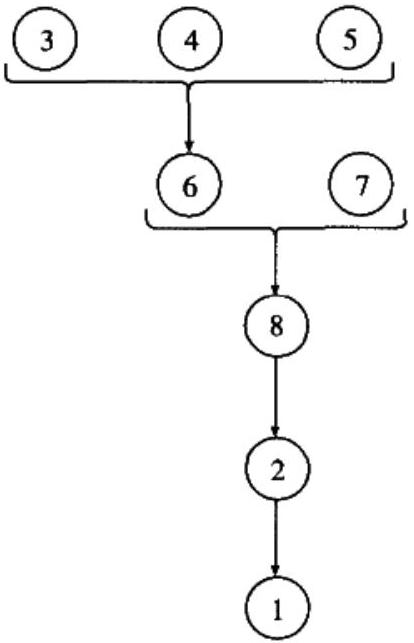
\includegraphics[max width=\textwidth, center]{2025_05_15_6a28331d5e7c993ad07ag-074}

在我们分析复杂的论证性话语时,即使是一些包含许多前提和分结论的语段,我们也经常发现它们是非常融贯的、清楚的。请看一位女编辑为其引起争论的编辑方针进行辩护时所写的一段话:

本刊(《新英格兰医学杂志》)的主张是(1)不发表不道德的研究报告,忽略它们的料学价值……

我们的主张有三个理由。首先,(2)如果普遍坚持这个主张,只发表合乎道德的研究文章,将会阻止不合乎道德的研究工作的开展。(3)文章的发表是医学研究奖赏制度的一个重要部分。(4)如果研究者知道他们不合乎道德的研究成果不能发表,他们就不会去做不道德的研究。(5)而相反的做法将有助于导致更多的不道德研究工作的开展,因为,如我已表明的,(6)这样的研究可能比较容易开展,因而(7)可能使从事不道德研究工作的人处于有利的竞争地位。其次,(8)即使发表不道德的研究成果不妨碍发表合乎道德的研究成果,为了坚持把合乎道德放在研究第一位的原则,也应该拒绝不道德的研究。(9)如果允许有所松动,我们将逐渐变得习惯于发表不道德的研究成果,并且(10)这将导致对发表合乎道德的研究成果的极大妨碍。最后,(11)对不道德研究成果的拒绝,有利于使社会普遍注意到,甚至某些科学家也不懂得科学研究应是文明的基本尺度。(12)知识尽管很重要,但对一个公平公正的社会来说知识或许远不及得到知识的方法重要。 ${ }^{[52]}$

最后的结论也出现在语段开头,(2)、(8)和(11)三个主要命题直接支持这个结论,这三个前提本身又得到处于不同位置的其他几个前提的支持。语段中的众多命题,在导出结论的过程中都有一个清楚的逻辑作用,共同服务于整个语段要证明的结论:不合乎道德的研究报告将不能在《新英格兰医学杂志》上发表,它们的科学价值也应被忽略。下页的图示展示了这个虽然复杂但推理缜密的语段的逻辑结构。

日常生活中的论证经常达不到这样的水准。它们可能包含着作用不清楚的陈述;论证中陈述与陈述之间的连接可能相互纠缠或被错述;甚至在论证者的头脑中论证的流程可能本来就是混乱的。由图示支持的逻辑分析\\
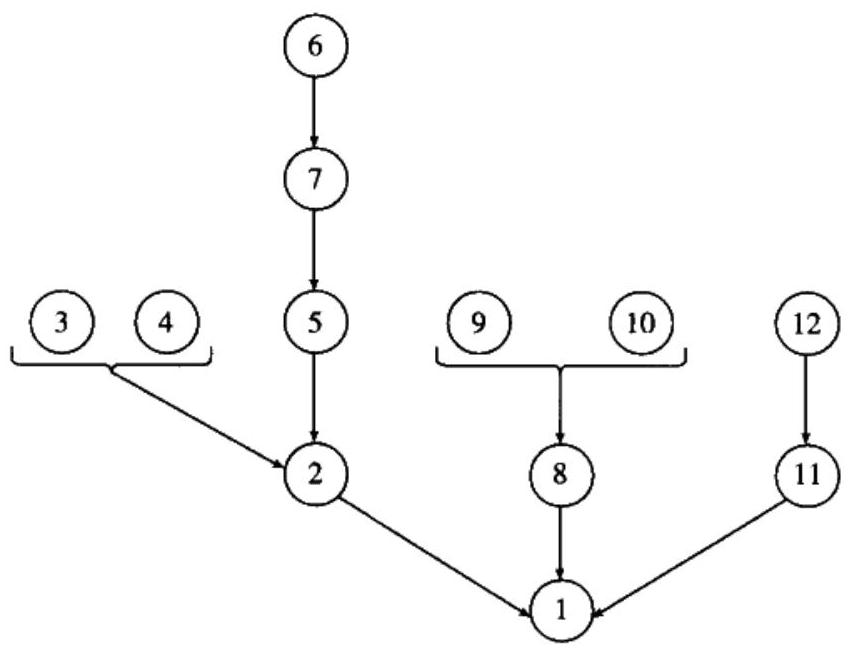
\includegraphics[max width=\textwidth, center]{2025_05_15_6a28331d5e7c993ad07ag-076}

可以暴露这些不足。通过使一个推理过程的结构暴露出来,我们能看到推理过程是如何展开的,推理的长处与缺陷是什么。逻辑学的一个特殊领域就是对实际论证的评估,成功的评估需要对所分析的论证有一个清楚的把握。 
\section*{1.11 推理}
如前所述,逻辑学是研究用于区分正确推理与不正确推理的方法和原理的学问。推理与论证都是从已知的(或为了某种目的而肯定的)前提推出结论的过程。至此,我们一直在分析和评估的是别人的论证。当然,我们在决定自己应如何行动、评价他人的行动、为道德的或政治的信念进行辩护等方面,我们每天都要建构我们自己的论证。建构和运用好的论证之技能是有巨大价值的。

推理的技能可以通过训练来提高。为了促进这样的训练,许多推理游戏(例如国际象棋、围棋、Mastermind ${ }^{(1)}$ 等)都是极好的手段。而那些用以强化和测试我们的逻辑技能的推理谜题,也无疑是相当实用的。推理不仅是一项必要的活动,也是一项愉快的活动——当我们解决了为提高技能和使人娱乐双重目的而设计的一些逻辑问题时,它所产生的乐趣是不言而喻的。

人为设计的问题比现实生活中的问题更简洁,通常也更简单。但是解答它们是具有挑战性的,经常需要锲而不舍地反复推理,这在思考模式上与侦探或新闻工作者或陪审员没有很大不同。可能需要找到一个推理系列,在这个系列中,所得的次结论被用做后来推理的前提。也可能要求具有一定的洞察能力,要找到解决问题的路径需要对早先假设或发现的信息进行创造性的重组。解决人为设计的问题往往是比较困难的,有时会无功而返,但是当通过推理的成功应用解决了问题时,是非常令人满足的。逻辑游戏和谜题解答,伴随各种推理模型的运用,都是很好的娱乐。"对思虑的享受",美国哲学家约翰•杜威写道,"是受过训练的大脑的标志"。

推理问题的一个常见类型是智力测验,仅仅使用所提供的线索,我们被要求理清和辨识有关的几个人物的名宁,或角色,或其他事实。下面是一个比较简单的例子:

在某个航班的全体乘务员中,飞机驾驶员、副驾驶员和飞行工程师的职务由爱伦、布朗和卡尔三人担任,但不必是这个

\footnotetext{(1)种著名的网络智力游戏。
}次序。\\
副驾驶员是个独生子,钱挣得最少。\\
卡尔与布朗的姐姐结了婚,钱挣得比驾驶员多。\\
问:三个人每人担任什么职务?

为了解答这样的问题,我们首先要寻找一个范围,在这个范围中我们 59 有足够的信息去得到超出前提所给信息的一些结论。我们从前提中知道许多关于卡尔的情况:他不是飞机驾驶员,因为他挣得比驾驶员多;他也不是副桇驶员,因为副驾驶员挣得最少。通过排除我们可以推出,卡尔一定是飞行工程师。

使用上述的次结论,我们可以确定布朗的职务。布朗不是副驾驶员,因为他有一个姐姐而副驾驶员是个独生子;他也不是飞行工程师,因为卡尔是飞行工程师。所以布朗一定是飞机驾驶员,而仅剩的爱伦一定是副驾驶员。

在解答这类问题(有时非常复杂)时,建构一个备选项的图示是非常有帮助的,这种图示叫做矩阵,当我们积累了新的信息时就把它填人表中。要见识这种矩阵图的作用,请考虑下面的问题:

阿伦佐、库特、鲁道夫和威拉德是四个天资极高的创造性的艺术家。一个是舞蹈家,一个是画家,一个是歌唱家,一个是作家,但不必是这个次序。\\
(1)那天晚上歌唱家在音乐会舞台上进行他的首次演出时,阿伦佐和鲁道夫在观众席上。\\
(2)库特和作家两人有画家为他们画的生活肖像。\\
(3)作家正准备写一本阿伦佐的传记,他写的威拉德的传记是畅销书。\\
(4)阿伦佐从未听说过鲁道夫。\\
问:每个人的艺术领域是什么?

将这些前提中断定的许多事实记在头脑中,也记住几个可以从这些前提推出的分结论,这是一项必需的工作。把我们的推论记在便条上可能是有帮助的,但是也可能导致混淆和零乱。我们需要一种有效方法,来贮备

已知的信息和所引出来的中间结论,能把已知的信息和推出的信息整齐地记录下来,并随着推论的数目不断增长以及论证的链条不断拉长供我们使用。而在我们要建构的矩阵表中就有空间去表示所有相关的可能选择,并能记录下每一个引出的推论。

这个问题的矩阵表必须是显示这四个人(用四行表示)和他们从事的四种艺术职业(用四列表示)的一个列阵,如下所示:

\begin{center}
\begin{tabular}{|l|l|l|l|l|}
\hline
 & 舞蹈家 & 画家 & 歌唱家 & 作家 \\
\hline
阿伦佐 &  &  &  &  \\
\hline
库 特 &  &  &  &  \\
\hline
鲁道夫 &  &  &  &  \\
\hline
威拉徳 &  &  &  &  \\
\hline
\end{tabular}
\end{center}

当我们断定名字在某行左边的人不可能是从事某列顶端所示职业的艺术家时,我们就在那个人名字的右边以那个职业做标题的列中空格写一个 N (代表"no",或写一个"一"符)。我们立即可以从前提(1)做出推断,阿伦佐和鲁道夫都不是歌唱家,所以我们在第三列(歌唱家)他们名字的右边空格写上一个 N。同样,我们可以从前提(2)推断库特既非画家也非作家,所以我们把一个 N 记在第二列(画家)和第四列(作家)他的名字右边的空格中。从前提(3)我们看出作家既非阿伦佐也非威拉德,所以我们把 $N$ 记在第四列他们名字右边的空格中。至此我们记录的所有项目都得到了原先所给信息的证明,现在的矩阵表如下:

\begin{center}
\begin{tabular}{|l|l|l|l|l|}
\hline
 & 舞蹈家 & 画家 & 歌唱家 & 作家 \\
\hline
阿伦佐 &  &  & N & N \\
\hline
库 特 &  & N &  & N \\
\hline
鲁道夫 &  &  & N &  \\
\hline
威拉德 &  &  &  & N \\
\hline
\end{tabular}
\end{center}

从已获得的信息我们可以用排除法断定,鲁道夫一定是作家,所以我们在第四列(作家)下鲁道夫名字右边的空格中记一个 Y(代表"yes",或记一个"+"符)。现在从列阵看,很明显,画家一定或是阿伦佐或是威拉德,并且我们在这里可以排除阿伦佐:鲁道夫有画家给他画的肖像(从前提(2)可知),阿伦佐从未听说过鲁道夫(从前提(4)可知),因此阿伦

佐不可能是画家。这样我们记一个 N 在第二列(画家)阿伦佐名字右边的空格中。

接着我们可断定阿伦佐一定是舞蹈家,从而在第一列(舞蹈家)阿伦佐名字右边的空格记一个 Y。现在我们可以在舞蹈家列中为库特和威拉德二人分别记人一个 N 。对库特来说剩下的唯一可能是歌唱家,所以我们记一个 Y 在那个空格中,并且记一个 N 在威拉德名字右边歌唱家列的空格中。再通过排除我们断定,威拉德一定是画家,并将一个 Y 填入矩阵表的最后一个空格。完成的图示是这样的:

\begin{center}
\begin{tabular}{|c|c|c|c|c|}
\hline
 & 舞蹈家 & 画家 & 歌唱家 & 作家 \\
\hline
阿伦佐 & Y & N & N & N \\
\hline
库 特 & N & N & Y & N \\
\hline
鲁道夫 & N & N & N & Y \\
\hline
威拉德 & N & Y & N & N \\
\hline
\end{tabular}
\end{center}

从这个填满的矩阵表中我们可以得到答案:阿伦佐是舞蹈家,库特是歌唱家,鲁道夫是作家,威拉德是画家。

当要求提供几种不同范围的答案时,这种综合性质的智力游戏就变得更复杂了。有些这样的问题非常具有挑战性,并且不使用矩阵方法几乎不可能解决。 ${ }^{[53]}$

另一些推理问题提出的是一种不同的挑战。下面是一个精致、娱人但不是很困难的问题。在阅读紧随其后的答案之前请努力解决它。

你面前有六个球:两个红球、两个绿球和两个蓝球。在每一对同色球中,你知道其中一个比另一个重。你还知道所有三个重球的重量相同,所有三个轻球也一样重。另外,这六个球(把它们分别叫做 R1、R2、G1、 G2、B1 和 B2)难以区分。你只有一架天平秤盘。

问:若在秤盘上称量不能超过两次,如何能辨认出所有三对球中的重球和轻球?

\section*{答案:第一次称量: $\mathbf{R 1 + G 1 / / R 2 + B 1}$}
如果两边平衡:R1 和 R2一对红球中,一个重一个轻。因两个红球分别在秤盘的两边,我们知道如果两边平衡,那么每一边的另一个球一定也是一重一轻——因为如果两个重球在同一边,这一边就一定沉下去。因此,我们知道两者必居其一:G1 重而 B1 轻,或者 G1 轻而 B1 重。

如果在第一次称量时两边平衡,那么第二次称量:G1//B1。无论这一次称量的结果是什么,所有球的轻重都可以辨认出来。

如果(在这次称量中)G1 沉下去,那么:\\
-G1 重(且 G2 轻),且\\
-B 1 轻(且 B 2 重),且\\
$\cdots \mathrm{R} 1$ 轻(且 R2 重)。\\
如果(在这次称量中)G1 升上去:(上述结论的)反面就是真的。\\
但是,倘使在第一次称量中 $(\mathrm{R} 1+\mathrm{G} 1 / / \mathrm{R} 2+\mathrm{B} 1)$ 两边不平衡将会怎样?假设 $\mathrm{R} 1+\mathrm{G} 1$ 沉下去。(如果 $\mathrm{R} 1+\mathrm{G} 1$ 升上去,随之答案就简单地倒转过来。)

我们知道在这种情况下 R1(在这一边的红球沉下去)一定是重的;因为如果 R1 是轻的,R2 就是重的;并且如果 R2 是重的,R1+G1 就不会沉下去。

因为 R1 是重的,下面三种联合体之一一定是如此这般:\\
(a)G1 是轻的,并且 B 1 是轻的;或者\\
(b)G1 是重的,并且 B 1 是重的;或者\\
(c)G1 是重的,并且 B1 是轻的。

\section*{如果 $\mathbf{R 1 + G 1 ~}$ 在第一次称量中沉下去,第二次称量: $\mathbf{R 1 + R 2 / /}$ $\mathrm{G} 1+\mathrm{B} 1$ 。}
我们已经知道 R1 是重的。在这第二次称量中,R1+R2(重 + 轻)一定是下列两种情况之一:沉下去或升上去,或者两边平衡。无论是哪一种结果,我们都可以辨认出所有球的轻重如下:\\
(x)如果 R1+R2 沉下去,G1 和 B1 一定都是轻的(因为一个重的加一个轻的会在重量上超过仅仅两个轻的相加)。在这种情况下联合体一定是上面的(a)型:G1 是轻的且 B1 是轻的一一所有问题都被解决。\\
(y)如果 R1+R2 升上去,G1 和 B1 一定都是重的(因为重+轻在重量上只能被两个重的相加超过)。在这种情况下联合体一定是上面的(b)型:G1 是重的且 B1 是重的——所有问题都被解决。\\
(z)如果两边平衡,G1 和 B1 也一定是重+轻。在这种情况下联合体一定是上面的(c)型:G1 是重的且 B1 是轻的一一所有问题都被解决。

将这个问题推荐给你的朋友们之前,请练习说明上述答案!\\
在现实世界中,我们经常被要求从某个当前事态推出它的起因,从事

情现在是什么推出其过去是什么。科学家——特别是考古学家、地质学家、天文学家、医学家——通常面对着探究其起源的事件或条件。企图说明事情为何从过去的状况发展到现在的状况的推理叫做回溯分析。例如,令天文学家惊奇的是,1996年在地球旁边疾驰而过的彗星海库塔克(Hy- akutake)放射出比任何一位科学家曾预言的一颗彗星能够放射出的强 100倍的可变 X 射线。德国马克斯-普朗克研究所的一位彗星专家评论说: "为了研究这些数据,我们中断了我们正在进行的工作——但这是一种你喜欢拥有的问题。"

我们确实喜欢拥有这样的问题。因此,回溯分析问题经常是为娱乐而设计的。然而这样的问题也有一种特殊的困难:由科学的或历史的知识提供的现实世界的逻辑框架一定是以某种方式由问题自身规定的。一些规则或规律一定是在逻辑分析能够进行的范围内提出的。

棋盘是一种最著名的回溯分析问题的装置,而下棋规则规定了必要的 63 理论语境。下棋无须什么技术,但对(国际)象棋规则不熟悉的读者可以跳过如下例示。

象棋中的回溯问题通常采取这样的形式:棋盘中棋子的安排是给定的,对一局棋赛进行回溯分析,以比赛中遵守了所有比赛规则为前提。例如,图 1-1 代表一局棋赛所得到的形势,比赛中所有的着数都与象棋规则一致。那么,刚刚走的一着棋或几着棋是什么?\\
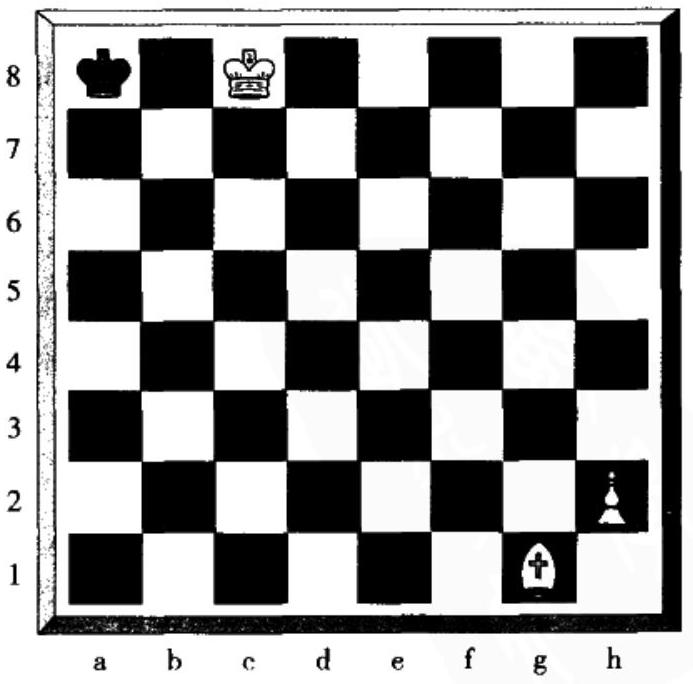
\includegraphics[max width=\textwidth, center]{2025_05_15_6a28331d5e7c993ad07ag-085}

图 1-1

为便于分析,所有行数从下到上加标数字 1 到 8 ,所有列数从左到右加标字母 a 到 h。那么棋盘中每一个方格都能用一个唯一的字母一数字结合体表示:黑王在 $a 8$ ,白兵在 $h 2$ ,等等。问题是:上一步由黑棋走的那着棋是什么?那么黑棋的前一步白棋的着数是什么?你能在阅读下一段之前推出答案吗?

答案:刚走的一着棋是黑王移动。因为两个王永远不能走在邻近的方格里,黑王不可能刚从 b7 或 b8 走到现在的位置上;因此我们可以确定黑王刚从 a 7 走到现在的位置,在 a 7 处黑王被将军。

这是非常容易推断的。但是前一着白棋是什么才能使黑王处于被将军的局面呢?那着棋不可能是白象(在 g1),因为白象没有一条路径能走到 g 1 格,不可能在白象走棋时黑王正处于被将军的局面!因此一定是,黑王被将军的局面是由另一个白棋子的移动造成的,这个白棋子正阻挡着象的攻击,并被走到 $a 8$ 的黑王吃掉。什么白棋子能在黑对角线上并且从那儿走到角上的白格中呢?只有在 $b 6$ 的马。所以我们可以确定,在黑棋最后一着(黑王从 a 7 到 a 8 )之前,白棋最后一着是从 $b 6$ 到 a 8 的马。 ${ }^{[54]}$

当然,现实生活中我们所面对的推理问题很少像本节所讨论的谜题这样整洁。许多现实问题的叙述不是很精确的,对它们的错误描述易于使人误解,从而不能得到答案。遇到这种情况,原问题的部分陈述就要加以拒绝或替换。而当我们试图解答本章给出的这种逻辑谜题时,我们是不能这么做的。

此外,现实世界中的一些问题,甚至当它们被准确描述时,也可能是不完善的,其中某个最初不是可供利用的条件,可能对于问题的解决是必不可少的。现实世界中一些问题的答案可能依赖于某个新的科学发现,或某个以前不可想象的发明或装置,或对某个至今未加探索的领域的研究。但是在逻辑谜题的陈述中,如同一部好的谋杀案侦探小说一样,必须给出足以得到答案的全部信息;否则我们就会认为侦探小说作家,或问题的设计者对我们是不公平的。

最后,逻辑谜题提出的问题都是清楚明确的(诸如:四个艺术家中哪一位是歌唱家?黑棋和白棋的最后一着是什么?等等),给出其答案并加以证明,就明确解决了逻辑谜题提出的问题。但那不是许多现实世界中的问题所呈现的形式。现实问题最初经常是仅仅由于某种前后矛盾的情形或一个不平常的事件的出现而被发现的,甚或只是基于人们对某种事情之不

顺畅的感觉而发现的——现实问题不是有着明确答案的精心构造的问题。\\
不管有多少区别,现实世界中的问题与精心设计的逻辑问题一样,都必须通过系统的推理才能得到解决,二者在逻辑学研究中都具有重要的作用。

\section*{第1章概要}
本章引进并举例解释逻辑学最基本的概念。

1.1节将逻辑学定义为研究用于区分正确推理与不正确推理的方法和原理的学问,并对这个定义作了阐释。\\
1.2 节阐释命题概念——命题是可以被肯定或否定,并且或真或假的东西——并且对命题与表示命题的语句作了区分。\\
1.3 节引人并阐释论证概念——串命题,其中之一是结论,另一个 (或一些)是用以支持结论的前提。\\
1.4 节说明并且例示分析论证的方法——一种是解析法,按照逻辑的顺序完整地列出论证中所有的命题;另一种是图示法,所有命题都用数字标示,这些数字以一定的方式相互连接以展现命题之间的逻辑关系。\\
1.5 节讨论辨识论证的几个方面的问题,包括结论指示词和前提指示词、语境在辨识前提和结论中的作用、有可能充当前提的非陈述形式以及包含未明确陈述出来的命题的论证等。

1. 6 节讨论论证和说明之间的区别,解释为什么做出这种区分常常是困难的,这种区分依赖于语段的语境和作者的表达意图。\\
1.7 节讨论演绎和有效性,将演绎论证定义为断言其结论从前提必然地得出的论证,一个有效的演绎论证就是一个假如其前提为真则结论必然为真的论证。\\
1.8 节讨论归纳和或然性,将归纳论证定义为其结论具有某种或然性程度,但并非(从前提)必然地得出的论证,说明归纳论证可以被判定好与坏,但不能刻画为有效与无效。\\
1.9 节讨论演绎论证的有效(或无效)与命题的真(或假)之间的某些复杂关系。

1. 10 节讨论复杂的论证语段,表明如何使用图示技术对它们进行分析。\\
1.11 节讨论推理问题,展示了一些能够训练与强化推理技术的方式,以及它们所提供的纯粹的智力快乐。

\section*{【注释】}
[1]William L.Shirer,The Rise and Fall of the Third Reich(New York:Simon and Schuster,1960).\\
[2]Abraham Lincoln,annual message to Congress, 3 December 1861.\\
[3]Voltaire,Epitre a l'Auteur du Livre des Trois Imposteurs, 10 November\\
1770.\\
[4]David Hayden,"Thy Neighbor,Thy Self",New York Times, 9 May 2000.\\
[5]"Ban Cigarettes",Orlando Sentinel, 27 February 1992.\\
[6]Jeremy Bentham,Principle of Legislation, 1802.\\
[7]Richard Zare,"Big News for Earthlings",New York Times, 8 August 1996.\\
[8]William Langewiesche,Sahara Unveiled:A Journey Across the Desert(New York:Pantheon Books,1996).\\
[9]标星号的练习的答案在本书结尾部分。\\
[10]Adapted from Alan Feduccia,The Origin and Evolution of Birds(New Ha- ven,CT:Yale University Press,1996).\\
[11]G.H.Hardy,A Mathematician's Apology(Cambridge University Press, 1940).\\
[12]R.S.Root-Bernstein,"Misleading Reliability",The Sciences,March 1990.\\
[13]这种技法是由几个知名逻辑学家多年前发明并完善的:Monroe C.Beardsley, in Practical Logic(Prentice-Hall,1950);Stephen N.Thomas,in Practical Reasoning in Natural Language(Prentice-Hall,1973);Michael Scriven,in Reasoning (McGraw-Hill,1976)。故本技法乃师法前人。\\
[14]James Rachels,cited in T.A.Mappes and J.S.Zembaty,eds.,Social Ethics, 3d ed.(McGraw-Hill,1987).\\
[15]Blanchard Hiatt,University of Michigan Research News,September 1979.\\
[16]A.J.Ayer,"Freedom and Necessity",Polemic,no. 5.\\
[17]Karl Marx,Letter \textbackslash #141, 9 April 1870,Karl Marx and Friedrich Engels Correspondence,1846-1895(International Publishers,1936)。(这封信并不是马克思写给恩格斯的,而是写给另外两人的。——译者注)\\
[18]Boston Women's Health Book Collective,Our Bodies,Our Selves(Simon and Schuster,1984).\\
[19]C.A.Quadir,Philosophy and Science in the Islamic World(London:Croom Helm,1988).\\
[20]Thomas Aquinas,Summa Theologiae,I,Question 96,Article 2,circa 1265.\\
[21]Ibid.,Article 3.\\
[22]From Science, 26 May 1995.\\
[23]Lois Taylor,"Is Smoking About Choice?"New York Times, 5 September 2000.\\
[24]D.C.Leven,"Deterrence Fails",New York Times, 3 March 1995.\\
[25]D.J.Amy,"Elections in Which Every Vote Counts",The Chronicle of High-\\
er Education, 12 January 1996.\\
[26]Freeman v.Pitts, 503 U.S.467, 1992.\\
[27]D.Goldin,"Some College Costs Should Be Tax Deductible",New York Times, 18 April 1992.\\
[28]A.Schopenhauer,"On Suicide", 1851.\\
[29]Plato,Meno,78a.\\
[30] 1 John 4: 20.\\
[31]Ramsey Colloquium of the Institute on Religion and Public Life,"Always to Care,Never to Kill",Wall Street Journal, 17 November 1991.\\
[32]William Shakespeare,Hamlet,act 1 ,scene 3 .\\
[33]Peter G.Brown,"Stardust",The Sciences,August 1988.\\
[34]该案例是指 Dickerson v.United States(No.99-5525),其中心议题(在 2000年4月19日口头辩论中)系关于国会是否有权通过法规超越米兰达规则。\\
[35]Anais Nin,Cities of the Interior(Denver,CO:Swallow Press,1959).\\
[36]William Shakespeare,Julius Caesar,act 3,scene 2.\\
[37]在后面 7.5 节将从另一个角度对省略三段论进行讨论。\\
[38]William L.Miller,Arguing About Slavery:The Great Battle in the United States Congress(Knopf,1995).\\
[39]引自堪萨斯州参议员 Sam Brownback 在2000年4月参议院就计划同意筹措这笔资金的议案举行的一次听证会上的发言。这个议案由他的共和党同僚、宾夕法尼亚州参议员 Arlen Specter 提交。\\
[40]又如,著名精神病学家、Dachau 和 Buchenwald 集中营的幸存者 Bruno Bettelheim 说:"如果所有人都是善良的,那就不会有奥斯威辛集中营了。"\\
[41]前提指示词"因为"(since)常常也含有时间的意义。例如,在著名的抒情老歌"Stormy Weather"中,"Since my man and I ain't together,keeps rainin'all the time"这一行有意含混,让人充满联想(Harold Arlen 作曲,Ted Koehler 作词, 1933)。\\
[42]"巴别"(Babel)一名取自希伯来语,意为"变乱",即以不分青红皂白的方式把事物混淆、堆积在一起。\\
[43]Jeff Greenwald,"Brightness Visible",New York Times Magazine, 14 May 2000.\\
[44]Andrew Porter,in a review of James's The Rise and Fall of the British Em- pire(1995),in the New York Times Book Review, 14 January 1996.\\
[45]Andy Rooney,New York Times, 29 April 1996.\\
[46]在日常语言中,词项"有效的"和"无效的"有着较宽泛的和不严格的含

义。但是作为逻辑学家,我们是在非常狭窄的意义上使用"有效的"和"无效的"这两个词项的;它们除了表明演绎论证在断定如果其前提是真的则其结论必定是真的这一点上是成功的或是不成功的以外,不表示任何别的意思。\\
[47]例如,如果我们知道三次抛掷一枚硬币连续出现三次正面的或然性是 $1 / 8$ ,我们就可以演绎地推知三次抛掷一枚硬币得到至少一次背面的或然性是 $7 / 8$ 。\\
[48]Abraham Lincoln,in Roy R.Basler,ed.,The Collected Works of Abraham Lincoln,vol.3.Rutgers University Press.\\
[49]Science,Medicine,and Animals,National Academy of Sciences,Washing- ton,DC, 1991.\\
[50]Eric J.Lerner,"For Whom the Bang Tolls",New York Times, 3 June 1991.\\
[51]Victor Wouk,"You Can't Drive Solar Cars to Work",New York Times, 15 July 1991.\\
[52]Dr.Marcia Angell,"The Nazi Hypothermia Experiments and Unethical Re- search Today",New England Journal of Medicine, 17 May 1990.\\
[53]能从这种逻辑问题中找到乐趣的读者会从 Original Logic Problems 丛书中获得极大的享受,其出版者为 The Penny Press,Norwalk,CT。\\
[54]在回溯分析问题中找到乐趣的读者定会在汇集此类问题的一本书中找到更多的快乐。该书由逻辑学家 Raymond Smullyan 编辑,书名 The Chess Mysteries of Sher- lock Holmes(New York:Alfred A.Knopf,1979)。

% others

% 第二部分
% 本章导言
\begin{quote}
\textit{命题逻辑是研究命题之间的逻辑关系和演算的基础。本部分介绍命题逻辑的基本概念和方法,包括真值表、逻辑连接词和形式系统等内容。}
\end{quote}

\section*{2.1 语言的三种基本功能}
语言是一种非常精细和复杂的工具,以至于我们可能会忽视它的用法 (uses)的多样性。我们会自然而然地去追求简单化,而不注意语言使用的语境及其不同使用目的,从而就可能被我们遇到的语词或者话语形式所误导。

语词并不总是服务于它们的表面诉求。在非正式谈话中,"你好吗?"这个问题并不是真正地在询问他人的健康状况。虽然这句话好像是在进行信息请求(a request for information),但是我们知道,它通常仅仅是一句友好的问候。那些通过描述其健康状况来回答该问题的人,就很可能被认为是愚義的。请求、报道和问候等仅是语言所具有的一些比较明显的功能。

哲学家乔治•贝克莱(George Berkeley)在他的《人类知识原理》 (Treatise Concerning the Principle of Human Knowledge)(1710)中说:\\
……思想交流……并非像通常想象的那样是语言的首要的和唯一的目的。使用语言还有许多其他宗旨,诸如引起某些情感、鼓动或者抑制行动、使人专心于某些特定的安排等等。前者(交流思想)在很多情况下都基本上是从属性的;当没有前者也能实现那些宗旨时,前者甚或完全被忽略,我认为,这种情况在人们熟悉的语言用法中经常发生。

20世纪的哲学家们非常详尽地阐明了多种多样的语言用法。路德维希•维特根斯坦(Ludwig Wittgenstein)在其《哲学研究》(Philosophi- cal Investigations)(1953)中正确地主张,"我们称之为'符号'、'语词'和'语句'的东西有无数不同种类的用法。"在维特根斯坦所列举的例子中有:发出命令、描述物体的外表或者给出它的测量结果、报道事件、推测事件、提出和检验假说、结合图表提交实验的结果、编故事、演戏、唱歌、猜谜、开玩笑、解算术题、语言翻译、询问、思考、诅咒、问候和祈祷等等。

语言的用法多得令人吃惊,通过将它们分为三种非常笼统的种类,即

信息性用法(the informative)、表达性用法(the expressive)和指令性用法(the directive),可以使之具有一定的条理。诚然,这种三重划分是一种简化,甚或过于简化。但是,许多逻辑和语言学者发现这是一种非常有用的划分。

1.语言的第一种用法是用于信息交流。通常,它是通过明确表述并肯定(或者否定)命题来完成的。能被用于肯定或否定命题,或者能为此提出论证,称为语言的信息性功能。这里使用的"信息"一词也包括错误信息,即既包括真命题也包括假命题,既包括错误的论证也包括正确的论证。信息性话语用来描述世界和进行有关世界的推理。无论其所报道的事实重要与否、是普遍还是特殊,用来描述和报道的语言都是用来提供信息的。下面就是一个语言的信息性用法的简单例子,它出自最近佛罗里达高等法院的一篇报道:

\begin{displayquote}
2000年11月7日,星期二,佛罗里达州,和美国其他州一道,进行美国总统普选。11月8日,星期三,该选举分区(佛罗里达州)报道说,共和党候选人乔治•布什获得 2909135 张选票,民主党候选人小艾伯特•戈尔获得 2907351 张选票。因为投给他们的全部票数的总差(1784张),低于该选区全部投票票数的百分之一的一半,所以根据佛罗里达州法律规定进行了自动重新计票。 ${ }^{[1]}$
\end{displayquote}

2.正如信息性话语的最为清晰的例示来自于法院或者实验室的报道一样,语言用做表达性用法的最好的例子来自抒情诗。面对令人惊奇的古城帕特拉(Petra)遗迹,约翰•W•伯根(John W.Burgon)的诗句:

\begin{displayquote}
如此奇迹今我惊叹,它保留在东部的风情中——玫瑰一样红的城市——"几乎和时间一样永恒"!
\end{displayquote}

并不是意欲告诉我们关于世界的任何事实和理论,而是要表达诗人的赞赏和敬畏之情。这些诗句告诉了我们他眼前的一些真实景色,但是它们的主要目的并不是为了报道信息。诗句表达了作者感受到的强烈情感,其目的在于在读者心灵中激起类似的情感。无论何时,如果语言被用来发泄和激

发情感,那么它就具有表达性的功能。\\
"表达"这个词在这里的运用范围比通常要狭窄。很自然,我们可以说表达感情、情感或态度等。但是通常情况下,人们也可以说表达见解、信念或者信仰。为了避免混淆语言的信息性的和表达性的功能,我们将说陈述或表明见解或信念,而在本章中将"表达"这个词留用于揭示或交流情感、感受和态度。

并非所有的表达性语言都是诗歌。我们用"真糟糕"或"真遗憾"来表达悲伤,用"好极了"或"太妙了"来表达兴奋。强烈的情感可以通过恋人爱慕的喃喃私语来表达。崇信上帝者,通过诵读主祷文或大卫王的赞美诗第 23 篇,可以表达他对广袤无垠和神秘莫测的宇宙的敬畏和惊叹之情。语言的这种用法不在于交流信息,而在于表达情感、感受或态度。正因为表达性话语只是表达性的,故而其既不真也不假。若把真与假、正确与错误作为衡量抒情诗之类的表达性话语的标准,那就会文不对题,使其价值丧失殆尽。谁要是因为知道是巴尔波(Balboa)而不是柯尔特斯 (Cortés)发现了太平洋,而降低对济慈(Keats)的十四行诗《初读查普曼译荷马》(On First Looking into Chapman's Homer)的欣赏,那他就是一个蹩脚的读者。这首诗的宗旨并不是教给人们历史知识。当然,有些诗的确含有重要的信息性内容。在伟大的诗人那里,有些诗的确是很好的 "生活评判"。但是,这种诗就不仅仅是表达性的了。可以说,这种诗具有 "混合用途"(mixed usage)或曰包括多种功能。这个概念将在后面作进一步讨论。

表达可以分成两种情形。当一个人独自发泄,写诗却不视之以人,或者孤独地祷告时,他的语言就起到表达说话者或写作者情感的功能,但不是为了在别人心中引起共鸣。另一方面,当演讲者要寻求感染他人时,当恋人在求爱中使用诗歌语言时,以及当人群为运动队欢呼时,语言就不但被用来表示说话者的情感,而且还意欲在听者心中引发共鸣。总之,表达性话语或者用来表达说话者的情感,或者用来激发听讲者的情感共鸣。当然,它也可以同时具有这两方面的功用。

3.当语言意欲引起或阻止明显的行动时,它就具有了第三种功能,即指令性功能。其最显然的例子就是命令和请求。当父母告诉孩子洗手吃饭时,其意图不是为了交流任何信息或者表达或激发任何特殊情感。这种语言是为了获得其指令结果。当你去电影院对售票员说"请给两张"时,

语言也是被指令性地使用以产生行动。命令和请求之间的差别是微妙的,因为通过语调的适当转换,或仅仅是加上"请"这个词,几乎所有的命令都可以变为请求。通常,当提出问题以寻求回答时,该问题也被归类于指令性话语。

在单纯的祈使形式中,指令性话语既不真也不假。一个命令,比如 "关上窗户",既不能是真的也不能是假的。对一个命令是否应当遵从,我们可能会有不同意见;但是,对命令是否有真假,我们不会有分歧,因为真假这样的词语不能直接运用于命令句。不过,命令和请求还具有其他属性——合理或不合理、适当或不适当——这些属性与信息性话语的真或假有相类似之处。在第1章中我们看到,我们可以为履行某个行动给出理由,而如果陈述这些理由时伴随着命令,那么我们就可以把整个过程视为论证。例如:

\begin{displayquote}
小心驾驶!谨记墓地中满是守法的公民,他们有走路的权利。 ${ }^{[2]}$
\end{displayquote}

在把这种话语处理为论证时,我们可以把其中包含的命令视做命题。命令的接受者从中被告知他们应当或应该履行所命令的行动。有些学者研究了这类问题,已经发展出了"祈使逻辑"(logic of imperatives),但对它的讨论超出了本书的范围。 ${ }^{[3]}$ 
\
\\section*{2.2 多功能话语}
前面所给出的信息性的、表达性的和指令性的话语的例子,打个比方说,都像纯正的化学标本。语言交流的这种三重划分是启发性的,有价值的,但是不能机械运用,因为几乎任何一种正常交流都可能会表现出语言的这三种用法。例如,一首诗可能主要是表达性话语,但也可能会有教育意义并因而也可以引导读者走向不同的生活方式。华兹华斯(Words- worth)写道:

我们身边的世界丰富精彩:迟早,无论是得到和失去,我们都要浪费掉自己的精力:

显然,诗歌也可以包含一定数量的信息。\\\\
再如,尽管布道主要是指令性的,希冀在会众中带来一定令人称赞的行动(抛弃罪恶,乐善好施),但是它也可以表达并激发情感,因而具有表达性功能,而且还可以包括一些信息,比如福音(the Gospels)的好消息。科学论文虽然本质上是信息性的,但是也可以表达作者的理性激情,而且还可以至少是含蓄地请读者去独立地证明作者的结论。语言的大多数平常的用法都是混合的。

语言的这种混合的或多功能的用法,并不是因为说话者或作者混淆了它们。相反,成功的交流都要求一定的功能结合。除清晰的语境和正式的关系——一父母与子女,雇主与雇员——之外,人们不能简单地发布命令并希望它得到执行。赤裸裸的命令会引起反感和敌对,并且经常是自生自灭。因此,必须使用一定的间接方式。通常,为了追求我们要引起的行动,我们并不直截了当地发布命令,而需要使用比较委婉的方法。

行动常常具有非常复杂的原因。与逻辑学家相比,心理学家更为适合研究动机,但是行动通常既涉及行动者的欲望又涉及他的信念,这是常识。除非饥饿的人相信他们面前的东西是食物,否则,他们就不会把它放进自己的嘴里;除非想吃,否则,即使人们毫不怀疑面前就是食物,他们也不会去碰它。

欲望是我们所谓的"态度"或"情感"的特殊类型,而信念通常会受到所接收到的信息的影响。因此,我们有时是通过激起他人的适当态度而成功地引起他们的行动,而有时则是通过提供信息以影响他们的相关信念而做到这一点。

假设你的目标是使你的听众向某个特定的慈善组织提供捐助,假定你的听众态度是助人为乐的,你就可以通过给他们提供该慈善机构的良好工作信息而促使他们行动。你的语言是指令性的,目的是引起行动,但你是通过提供信息,而不是通过发布一条毫无掩饰的命令或不客气的要求,而达到你的诉求的。再如,假定你的听众已经被深深地说服,相信我们谈论的那个慈善机构确实信誉良好,但对捐献的鲁莽要求仍然可能失败;但是,通过在一定程度上激发他们的乐善好施情感,你就可能会成功地使他们向该慈善机构提供捐助。在这种情况下,你就通过使用表达性的话语而

达到了自己的目的:你实现了一个"动人诉求"(moving appeal)。这样,你的语言自然而然地就具有了混合用法,既有表达性功能又有指令性功能。

最后,再假设你要向那些既缺乏乐善好施的态度,也缺乏对你推荐的慈善组织之信誉的认识的人进行捐献动员,那么你就必须一并使用语言的三种功能,既要有表达与信息功能,又旨在引发行动。这种一并使用并不是可偶尔为之的用法,而是必须为成功交流而精心准备的基本手段。

语言的三种基本用法是:信息性用法、表达性用法和指令性用法。但值得一提的是,语言在某些特殊语境中还具有一些特殊用法,而这些用法并不能完好地归属这三重划分。

语言的礼仪性用法是很普遍的,在有些场合下它是一种表达性的和指令性的话语的混合。社交中的问候、赴宴邀请、雇用告知等表述,都是体现礼仪功能的例子;语言还有很多其他相关的不确定用法,它们主要服务于使人们之间的互动变得融洽。礼仪功能还是宗教场合中一种庄重的语言用法。给人留下深刻印象的结婚仪式的语言,既要突出场合的庄重性(表达性的功能),又要使新郎和新娘提高对严肃的结婚誓言的正确理解而引起新的角色行为(指令性的功能)。

与礼仪性用法相近,语言还有其他一些用法,它们也不仅仅是那些主要用法的混合。假如有人邀请你在某一时间和地点去参加会议,你回答 "好,我答应你",那么你就不仅是以此表明了你的态度和预告了你的行为,你同时还用语言来许诺。相似的,在婚礼结束时,司仪或主持人说 "我宣布你们是夫妻",这也不仅是表明了说话者在干什么。在有些语境中,说出某些话实际上包含了一种重要行动。这些都是语言的践行性 (performative)用法的例子。

践行性话语实际上就是实施一种行动,即其所报告或描述的行动。践行性动词是一种特殊的种类,它们代表行动,这种行动通常是以第一人称使用动词而(在适当的情况下)完成的。这里可以再举出一些例子,如 "我祝贺你……"、"我向你道歉,我……"、"我建议……"、"我将这艘船命名为 $\\cdots \\cdots$"、"我接受你建议......"等等。

语词和语句的这些及其他的特殊用法显示了自然语言的丰富性,它们的诸多复杂功能难以归纳为任何一个单独的分类系统。 
\section*{2.3 话语形式}
语句常常被定义为表达一个完整思想的语言单位。在语法教科书中,语句一般被分为四种类型,即陈述句、疑问句、祈使句和感叹句。但是,这四种语法分类与陈述、询问、命令和惊叹并不完全对应。我们可能会尝试把形式等同于功能,即认为陈述句和信息性话语是对应的,感叹句仅仅适用于表达性话语,或者我们会认为指令性话语完全包括祈使句或疑问语气的句子(把询问总是当做寻求回答的请求)。假如这种整齐的等同是可能的,那么交流问题就会大大地简单化了,因为这样我们就可以仅仅通过一段话的形式而说出它的原有功能,而其形式是很容易直接检查的。但是,那些把形式与功能等同的人会错误理解别人的话,而且或许会漏掉别人要传达的很多要点。

设想任何具有陈述句形式的事物都是信息性话语,真的就予以好评, 77 假的就予以拒斥,这显然是不正确的。"我在你的聚会上度过了一段美好的时光"是个陈述句,但它的功能完全不必是信息性的;倒不如说,它是礼仪性的或者表达性的,表达了友好和欣慰的感情。尽管很多诗歌和祷文的功能都不是信息性的,但它们却具有陈述句的形式。简单地认为它们是信息性的并简单地将它们评价为真的或假的,将会把自己排除在富有价值的审美和宗教体验之外。同样,许多请求和命令都是间接地——或许更加委婉地———用陈述句来表述的。"我喜欢咖啡"这个判断句不应当被侍者仅仅当做是顾客的表白,而应当被视为针对行动的指令或请求。对于陈述句,诸如"对这些帮助,我将非常感谢"或"我希望你课后能够在图书馆见到我",假如我们僵硬地判别它们的真与假,只是将它们视为信息报道,那么我们很快就会没朋友了。这些例子向我们表明,陈述的形式并不一定就标朋信息性功能。陈述句在每种话语类型的表达方式中都能见到。

其他语句形式也是如此。"你意识到我们几乎要迟到了吗?"这个疑问句,不必是在询问你的大脑状态的有关信息,而可能是要求抓紧时间。疑问句"1939年,俄国和德国签署了一个条约,它导致了第二次世界大战,不是吗?"可能完全不是询问,而可能是交流信息的间接方式或者是企图表达并激发一种对俄国的敌对情感;在第一种情况下起的是信息性功能,

而在第二种情况下起的是表达性功能。甚至语法上的祈使句,如在公文中以"兹请周知 $\cdots \cdots$"开头,可能并不是命令,在其所断言的东西中是信息性话语;在其激发神圣和庄重的适当情感的语言用法中是表达性话语。就感叹句来说,尽管它与表达性话语的功能关系紧密,但也可以有相当不同的功能。感叹句"天啊,要迟到了!"在语境中可以表示抓紧时间的请求。而房地产经纪人对潜在的顾客说出"多么美好的景色啊!"这个感叹句,其祈使性功能比表达性功能更浓重。

许多话语都企图同时达到语言的两种或者可能是其全部的三种功能。在这种情况下,给定语段的每一方面或功能都从属于它自己的适当标准。一个具有信息性功能的语段可以具有能够评价为真或假的方面。同样的语段,也可以具有指令性功能,能够以恰当或不恰当、对或错等进行评价。而假如这个语段还具有表达性功能,那么其组成成分还可以评价为真诚或虚假、是否宝贵等。正确地评价某一给定语段,需要把握语言的不同功能以及该语段本身的宗旨。

对逻辑学家来说,真与假,以及与之相关的论证正确与错误的概念,是最重要的。因此,作为学习逻辑的学生,我们必须能够将信息性功能与非信息性功能的话语区分开来。进而,我们还必须能够理顺给定语段所具有的信息性功能与其可能具有的所有其他功能之间的关系。为了做到"理顺",我们必须知道语言可以具有哪些功能,以及必须能够将它们区分开来。语段的语法结构常常能够标示其功能,但是,功能与语法形式之间并没有必然联系。功能与语段表面上断言的内容之间也不存在严格的关系。关于这一点,一位大语言学家在他对"意义"(meaning)的讨论中给出了例证说明:

\begin{displayquote}
一个顽皮的孩子,该上床睡觉时却说"我饿了",他母亲知道他的把戏,就以打发他去睡觉来回答他。这是移位语(dis- placed speech)(1)的一个例子。 ${ }^{[4]}$
\end{displayquote}

在这里,这个孩子的话是指令性的一一虽然没有成功地实现其所希望的改变。关于语段的功能,我们一般是指它想要达到的那种功能。但不幸的

\footnotetext{(1)日常会话中的"托词"是"移位语"的一种典型,本处即为托词之例。
}是,那并不是总能够轻而易举地判定的。\\\\
当孤立地引用一个语段时,要判定该语段最初欲要达到的功能就特别困难。其原因在于,语境在判定功能的过程中极其重要。某些本身是祈使性或者普通信息性的语句,如果在实际语境中将它们安排到一个具有诗化效果的整体之中,就可以变为表达性语句。例如,孤立的:

到窗口来吧,

是一个起指令性功能的祈使句。而:

\section*{今夜海上风平浪静}
是陈述句,起着信息性功能。它们好像都没有较大的表达性威力,但是在马修•阿诺德(Matthew Arnod)的诗歌《多弗海滨》(Dover Beach)的语境中,二者都主要用为诗的表达性功能,而且效果显著。很多诗歌完全依赖于语段的表达性用法,而在其他语境中,这些语段却具有根本不同的功能。

下面的区分也是重要的,即句子表示的命题与关于说话者的事实(句子的说出就是证据)之间的区分。当有人说"天在下雨"时,这个被断言的命题是关于天气的,而不是关于说话者的。但做出断言却构成了说话者相信天在下雨的证据,这就是关于说话者的事实。也可能发生下述情况:人们做出的陈述只是表面上关乎他们的信念,实际上并不是为了给出关于他们自己的信息,而完全是一种述说其他事情的方式。如说"我认为黄金不应该用做货币的标准",通常并不能理解为关于说话者信念的心理自我表白,而只能理解为断言不应该使用黄金作为货币标准的一种方式。而当说话者发出命令时,由此推断说话者希望有人完成某事却是合理的;的确,在有些环境中,只要断言某人有某种特殊渴望,实际上就是给出了一个命令或者做出了一个请求。快乐地欢呼证明说话者非常愉快,即使他在整个过程中没有做出任何断言。但是,作为心理报道,断言说话者快乐就是肯定一个命题,这与只是快乐地欢呼相当不同。

在1.6节中我们注意到,论证与说明之间的差别常常取决于语段的说话者或作者的目的。现在,对语言的不同功能的探讨允许我们可以对该问

题进行更深人的考察。\\\\
当说话者论及某个有争议问题时,如果他说"我强烈反对什么什么",那么我们就理解,这样一句话的目的通常不是为了报道说话者的观点(除非这样的话是一位公职候选人或者其观点代表了公众利益的知名人士所讲的)。实际上,这种自我报道的表达形式是述说什么什么是个坏主意并且我们都应当反对它的常用方式。当说话者不断地证明我们所持的观点是正确的时候,他并不是在说明他的判断,而是有意的论证,以说服别人相信他的判断是正确的。对于有些争论性问题,通过陈述自己的观点而展开论证,并不是有意欺骗;在这种情况下,即使把判断和自我报道混合在一块儿,也不是有意欺骗。

在一个单独语段中,一种以上重要功能的组合可能会成为问题。思想表达,受我们宪法第一修正案的保护,可能会包含极具冒犯性的语言;在这种情况下,认识到冒犯言语中信息性与情感性功能的融合(integra- tion),对保护言论自由可能是极其关键的。在洛杉矶地区法院,一个年轻人身穿故意装饰有亵渎之物的夹克来抗议越战时期的军事法案;根据加利福尼亚刑法典,他以冒犯行为而被判处有罪。高等法院推翻了对他的指控,并雄辩地精确表述了这个问题:

我们不能忽视这个事实,这里牵涉的事件极好地表明,许多语言表达都具有双重交流功能:加上附带说明,它们不仅可以传达相当精确的思想,还可以传达其他不可表达的情感。实际上,与其情感力量一样,语词也常常因其认知力量而被选用。我们不能赞同这样的观点:宪法关注个人言辞的认知内容,而没有或不关心其情感功能。的确,情感功能可能常常是在寻求交流的信息的更重要因素……同样,我们也不能纵容这种轻率假定:可以禁止特殊言辞,但在这个过程中又不遭遇压制思想的真正危险。 ${ }^{[5]}$

区别语言的信息性以及论证性功能与语言的其他功能,并没有一个机械的方法。在后面几章中,我们发展的逻辑技术可以相当机械地运用于检验论证的有效性,但是没有一个机械技术可以识别论证的出现。识别在一给定语境中的话语的不同功能,要对语言的灵活性和其用法的复杂性熟虑

而敏感。\\\\
80

\begin{center}
\begin{tabular}{|l|l|}
\hline
语言的主要用法 & 语言的语法形式 \\
\hline
 & 陈述可 \\
\hline
信息性用法 &  \\
\hline
 & 疑问句 \\
\hline
表达性用法 &  \\
\hline
 & 祈使句 \\
\hline
指令性用法 &  \\
\hline
 & 感叹句 \\
\hline
 & 语法形式常常是功能的一个标志,但语法形式与其使用目的之间并没 \\
\hline
 & 定的联系。用做三种主要功能(左侧纵列)的任何一个功能的语言, \\
\hline
能会采用四种语法形式(右侧纵列)中的任何一种。 &  \\
\hline
\end{tabular}
\end{center} 
\section*{2.4 情感词汇}
现在,我们从讨论语句和较复杂的语段转向探讨构成它们的词汇。正如 2.2 节所见,一个单独的语句,可以同时具有信息性的和表达性的用法。要具有前者,句子必须明确表述一个命题,而要做到这一点,它的词

汇必须具有字面的或描述性的意义,以指示客体或事件以及它们的性质或关系。而当句子表达态度或感情时,其词汇就会具有情感的暗示或影响。一个语词或短语可以既具有字面意义又具有情感影响。后者通常被称为词汇的情感意义。

词汇的字面意义和情感意义在很大程度上是各自独立的。例如,"官僚"(bureaucrat)、"政府官员"(government official)与"公仆"(public servant)的字面意义几乎一样,但它们的情感意义却很有区别。"官僚"倾向于表达厌恶和反对,而作为敬语的"公仆"则倾向于表达尊重和赞赏。"政府官员"则更接近中性。

显然,我们用以指示事物的词汇会明显地影响我们对事物的态度。花的实际芳香不会因其名称而改变。正如莎士比亚所写的那样,一朵玫瑰不论使用其他任何名字,闻起来都是香甜的。然而,假如有人告诉我们有一种称做"臭菘"(skunkweed)的玫瑰,我们对它的反应就可能会受到影响。在华尔街(Wall Street),谨慎地选择语言可以促使人们在股票市场上采取行动。某几天是"回升",它意味着价格上涨;另几天是"取短期利息",这意味着价格在下降,因为很多人都在抛售股票,但这个词语仍然好听。如今大公司极少再进行"破产",但它们可以"重组",这听起来要好多了。

这种态度上的影响可以说明委婉语增多的现象,委婉语就是用温和的词汇表示严酷的现实。在战争中,己方军队的失败可能被称做容易接受的 "暂时撤退",而重大的撤退可能被报道为"兵力的有序集结"。在越南战争中,正在竞选总统提名的参议员尤金-麦卡锡(Eugene McCarthy)曾对美国的军事干预政策及公众不愿坦诚地面对它的状况进行了颇具讽刺性的批评:"我们不再宣称战争",他说,"我们宣称国家防御。"[6]

我们在不断地创造新词汇以替代那些不再令人满意的旧词汇。"殡葬人员"(undertake)变成了"殡仪员"(mortician),"看门者"(janitors)变为"守护员"(maintenance men),"老人"(old people)变成了"年长公民"(senior citizens)。但是,与旧的实际情况相联系的新替换的词汇最终也会失去它们的吸引力;"守护员"结果被"保卫者"(custodian)所代替,"殡仪员"为"殡仪主管"(funeral director)所取代,等等。杰梅恩•格瑞尔(Germaine Greer)写道:

\begin{displayquote}
经过与其指代的实际相联系,委婉语便迅速地失去了它们的功能,这是它们的宿命。因此,它们必须经常被它们自己的委婉语所取代。 ${ }^{[7]}$
\end{displayquote}

据说,杜鲁门总统的夫人贝丝(Bess)的朋友请求她阻止杜鲁门再说"大粪"(manure),她回答说,她花费了四十年时间才使他开始说"大粪"。

语言的确有它自己的生命,独立于它用以描绘的事实。有些包含生殖和排泄的生理活动可以用医学词汇不带情感地进行描述,而不至于引起神经质的不快;但是使用下流粗俗的词汇描述同样的活动却可以震惊除最麻木不仁者之外的所有听众。用我们的术语来说,可以说这两种词汇具有相同的字面或描述意义,但是在它们的情感意义上却有或缓和或激烈的对立。

在某个具体的人的思想中,词或短语有时可以产生情感意义,那不是产生于其字面上指代的东西,而是产生于第一次学习或遇到它的语境。一个作者曾描述说:

\begin{displayquote}
这是一个有启发意义的故事。一个小姑娘近来学会了阅读,正在拼读报纸上的一篇政治性文章。"爸爸,"她问,"什么是坦曼尼协会(Tammany Hall)?"她爸爸用通常社交禁语的口吻回答说:"亲爱的,你长大了就会明白的。"按照这种奇怪的成年人遁词,她终止了询问;但在她父亲的语气中,有某些东西使她相信坦曼尼协会必定与不正当的性事有关,以至于多年来她只要一听到这个政治机构 ${ }^{(1)}$ 就会体验到一种神秘的非政治性震颤。 ${ }^{[8]}$
\end{displayquote}

对于很多人来说,一定的词汇或短语,由于与我们的生活具有某些特殊联系,可以携带某种我们或许不愿公开承认的隐私情感。

字面意义和情感意义之间的对比,以及它们不同的可操作性用法,促使哲学家伯特兰•罗素设计了一种寓教于乐的游戏。他这样"调配"出一

\footnotetext{(1)坦曼尼协会最初是旨在通过捐赠与赞助进行控制的纽约市民主党执行委员会,成立于 1789 年。1805年转型为有明确政治宗旨的"慈着机构"。
}类"不规则动词"(irregular verb):

我坚定;你倔强;他头脑呆板。

伦敦的《新政治家和国家》(New Statesman and Nation)杂志随后举行了一次竞赛,以征求这样的不规则词汇表,获胜者如下:

我义愤;你生气;\\
他破口大骂。

我重新考虑过了;你改变了想法;\\
他食言了。

这种游戏证实了普通经验的教益:相同事物可以被情感色彩非常不同的词汇所指称。 
\section*{2.5 一致与歧见的种类}
任何事物或行动都可以选择不同的短语来描述:传达赞许或反对意见,或者中立意见;不同类型的一致(agreement)和歧见(disagree- ment)可以就任何事情展开交流。

两个人可能会在某事情是否已经实际地发生上意见相左,这种情况可称为"信念歧见"。另一方面,他们也可能都同意已经事实上发生了一件事,因而是信念一致的;但对那件事,他们仍可以具有不同的或者甚至相反的态度。你可以用语言描述那件事来表达赞许,别人却可以用语言来表达反对。这里也存在歧见,但不是信念歧见。这是对这件事的感受不同,

是态度歧见。 ${ }^{[9]}$\\
明确了这两种歧见,我们就可以区分出两个人(让我们把他们称做 A和 B)之间的四种关系,来讨论某些给定事件或者其他事实情况。

第一,他们可能达到充分一致,即他们对于事件发生的信念和对事件的态度都是一致的。

第二,他们可能对于事件的信念是一致的,但在态度上却对立,一个人认为是好事,而另一个人却认为是坏事。设想我们讨论的事件是:对于某个有争议问题,一位政治候选人的立场改变。对于的确发生了这个改变,A 和 B 可能意见一致;但是,A 认为好极了,而 B 则发现它令人担忧。如果像 A 所理解的那样,这位候选人就会被称赞为"倾听了理性的呼声";如果像 B 所理解的那样,这位候选人就将被谴责为"机会主义的反复无常"。

第三,他们可能态度一致,但对于引起态度的事实,他们却可能有信念歧见。因此,A 和 B 都可能热情地赞扬所论及的那位候选人,而他们对该候选人的实际立场却有不同理解。A 可能认为,由于"倾听了理性的呼声",那位候选人确实改变了他的立场;而 B 则可能认为,由于"坚定不移地拒斥了为奉承所左右",他根本没有改变自己的立场。乍一看,这个第三种可能性好像不合理,但经过思考之后就会被认为是平常的;我们知道,在政治选举中,同一候选人常常可能有不同的支持原因,这些原因不但不同而且有时还不相容。

第四,这两个人可能会处于一种完全对立的状态,他们不但在事实上有歧见而且对事实的态度也对立。由于相信那位候选人改变了立场,A 可能会非常热烈地称赞这种改变是"明智的重新考虑"的结果;由于认为候选人的立场保持未变, B 可能会激烈地贬斥他"顽固地拒绝承认错误"。

当我们以解决歧见为目标时,我们就必须既要关心给定情况下的事实,又要关心争论者对这些事实的不同态度。不同类型的歧见需要不同的解决方法。因此,如果我们不清楚所存在的歧见是什么类型,那么我们就不清楚去使用什么方法。信念歧见可以通过确认事实而得到最好的解决。为了明确这些事实,如果它足够重要,可以询问证人、查阅文本和检查记录等等。当事实得到了确证、解决了事实问题时,歧见就会得到解决。科学的探究方法在这里都可以用到,这将足以指导他们直面有关信念歧见的事实问题。

另一方面,如果是态度歧见而不是信念歧见,那么适于解决它的方法就有相当大的差别,难以如此径情直遂。以确证事件发生与否为目的,召唤证人、查阅文本,诸如此类,对解决这样的争论不会有什么效果,因为争论的问题并不是事实,这种歧见不是关于事实是什么而是关于怎样评价它们的对立。解决这种态度歧见的努力可能会涉及有关事实问题,但不是那种存在态度冲突的事实。或许考虑那种引出愉快或不愉快的结论的事情若不发生将会怎样,可能是有益的。动机和目的也可能具有重要性。诚然,它们都是事实问题,但如果歧见在信念上而不是在态度上,它们就都不会成为争论的主题。其他一些方法有时也可以解决态度歧见,你可以大量地使用表达性语言来尝试说服方法;在凝结团体意志和取得统一态度中,修辞艺术也可能富有成效(当然,它在解决事实问题上完全没有价值)。\\
"好"和"坏","对"和"错",诸如此类的语词,在严格的伦理用法中,往往具有非常强烈的情感色彩。无疑,当我们把某行动描述为对或把某情形描述为好时,我们就对它表达了一种赞赏态度。有些伦理学者认为,这些语词"没有"词汇意义或认知意义,而只有适合它们的情感意义;而另一些伦理学者则坚持这些语词的确具有认知意义,它们指称所讨论事物的客观特征。在这种争论中,学习逻辑的学生不必偏向某一方。但显然,不是所有的赞同或不赞同态度都蕴涵道德判断,因为还有审美价值的考虑,还有个人偏好或口味的影响。对某些事物(例如有些食品或服装款式)的否定态度,不必牵涉伦理或审美判断,但它也可以由情感色彩强烈的语言来表达。

当歧见是在态度上而不是在信念上时,最强烈的(当然也是实质的)歧见可以用朴实无华的真实陈述来表达。当双方针锋相对并以逻辑上相容的陈述来明确表述他们的分歧时,若认为双方的歧见不是"实质的"或者是"纯粹言辞的"就是错误的。他们并不是仅仅"用不同的言辞说相同的事物"。当然,他们可以用不同言辞来断言词汇意义上相同的事实,但是,他们也可以用不同言辞来表达对相同事实的矛盾态度。在这样的情况下,虽然他们的歧见不是"词汇意义上的",然而却是实质的。这不是"纯粹言辞的"歧见,因为语词既具有表达性功能也具有信息性功能。如果我们有兴趣解决歧见,我们就必须弄清楚其本性,因为适于解决一种歧见的技巧,正如我们已看到的,可能对另一种毫无用处。

有时,我们难以确定一种歧见是信念的或是态度的,或者既是信念的又是态度的;这可能取决于争论者对词汇的某种解说。冲突意见的表达方式可能会把不同态度之间的区别以及不同信念之间的区别弄得模糊,因此争论的关键核心就会难以把握。当两个人对在一个事物是否比另一个"更好"或"更重要"上意见对立时,他们都可能认为,真实情况很可能是不同信念使他们产生了分歧。但是在某些情况下,一个其表面形式是关于所谓的事实问题的差别论争,实际上是一个关于态度的实质争论,当争论的东西是事物或行为的价值时尤其如此。

在关于赢球的重要性上,一位著名体育运动作家和一位著名足球教练产生了深刻的分歧。新闻记者格兰特兰德•赖斯(Grantland Rice)写道:

\begin{displayquote}
当球星走进球场,为其声名留下光芒,这光芒不论输与赢,只记录场上飞奔的身影。
\end{displayquote}

文斯•隆巴蒂(Vince Lombardi)教练却说:

\begin{displayquote}
赢球不是别的,它就是唯一(竞赛目标)。
\end{displayquote}

很明显,这两位对赢球的态度是冲突的。你相信这种态度上的歧见的根源是信念歧见吗?

尽管有这些不可避免的困难,态度歧见与信念歧见之间的区分还是非常有用的;留心语言的不同用法有助于理解我们可能遭遇的种种歧见。当然,找出区别本身并不能解决问题或消除歧见。但是,由此可以澄清讨论的问题,揭示出它们的类型并找出冲突的所在。我们越充分地理解歧见的本性,我们就越能够更好地去解决歧见。 
\section{情感中性语言}

\begin{quotation}
\textit{在追求事实真相和理性分析时,情感中性的语言扮演着至关重要的角色。理解何时该使用情感语言、何时该避免情感色彩,有助于我们更有效地进行交流和推理。}
\end{quotation}

语言的表达性用法与信息性用法一样是正当的。情感语言本身没有什么不当,非情感语言或曰中性语言也没有什么不当。这就如同我们可以说枕头没什么错,锤子也没有什么错一样毋庸置疑。但是我们不能用枕头钉钉子,也不能枕在锤子上舒服地休息。同样,当我们用实话实说的话语来替换诗人的情感语言时,尽管可以保留罗曼蒂克诗句的字面意义,但它会失去很多兴味。在某些类型的诗歌中,情感色彩浓郁的语言比中性语言更受喜爱;而在另一些领域中,中性语言则比情感色彩浓郁的语言更为可取。

\subsection{中性语言在追求真理中的价值}

那是些什么领域呢?如果把探求现实真理作为我们的目标,那么\textbf{中性语言}就应更受重视。当我们试图了解事实的真相所在,或者试图加以论证时,心猿意马就会招致失败,而情感因素正是一种分散注意力的力量。激情倾向于掩盖理性,"冷静"(dispassionate)与"客观"(objective)两词接近同义的用法就反映了这个道理。因此,当我们试图以冷静和客观的方式推论事实时,使用强烈的情感语言便是有害而无益的。

\subsection{面对价值冲突的语言选择}

当我们处理某些冲突的话题时,使用完全中性的、不受感情影响的语言或许并不可行。例如,在流产是否正当的论辩中,论辩对手(无论哪一方)所使用的关键词汇就非常可能为情感所扭曲,因为此时并不存在完全不带情感色彩的所有各方都接受的价值中性词汇。在这种情况下,如果真正的目标仍然是求真,那么就应当尽可能地减少所用词汇的情感负荷。情感中性的目标不可能完全达到,但是我们至少可以尽力使用这种语言:它仅预设论辩者都赞同的信念(无论何种)。情感色彩的语言肯定是分散注意力的,情感意义负荷过重的语言是不可能促进求真的。

在论文《决定论的两难》(The Dilemma of Determinism)中,威廉•詹姆士(William James)提出"希望消灭"自由'这个词",其理由是"它的歌功颂德的联想……使它的所有其他意义黯然失色"。他更喜欢恰当地使用词汇"决定论"和"非决定论"来讨论"意志自由",他说,这是因为"它们冰冷的和数学的面孔没有情感牵连,而情感牵连可以预先以各种方式来贿赂我们"。詹姆士的做法为我们树立了榜样。

\subsection{民意调查中的情感陷阱}

从事专业民意调查的采访者必须非常谨慎,以免对调查询问中使用情感措辞而收到的反馈产生偏见。如果忽视这种慎重,调查结果就可能是没有价值的。1993年,《时代》(Time)和有线电视新闻网(Cable News Network)在一项大型民意调查中询问道:"应当通过立法来禁止利益集团赞助竞选吗?或者,利益集团的确应当拥有赞助他们支持的候选人的权利吗?"在所有回复者中, $40 \%$ 的人说他们赞同禁止利益集团的赞助, $55 \%$ 的人回答利益集团有赞助的权利。同年,罗斯-佩罗(Ross Perot),一位非常富有的总统候选人,组织了其自己的民意测验,其中如此询问: "应该通过立法来消除所有特殊利益者给候选人大笔金钱的可能性吗?"冊庸惊奇,对这个问题 $80 \%$ 的回答是"是的",这样的赞助应当禁止。包含像"特殊利益"和"大笔金钱"这样的短语无疑妨害了了解人们对这种事情的真实看法。$^{[11]}$ 可以说,这两个民意测验问的不是同样的问题。但即使如此,逻辑要点仍然是:如果我们的目标是交流信息,如果我们希望避免误会,那么我们就应该尽可能少地使用情感色彩浓厚的语言。

\subsection{警惕情感语言的操纵}

玩弄情感,而不是诉诸理性,是那些从歪曲真相中获得好处的人的常用手段。这种操纵的努力最公开的展示是广告世界,那里压倒一切的目的总是说服、销售并且常常是获利。我们必须经常警惕这些情感负荷的语言用法,也要警惕它们在政治活动中的使用,几乎每一种修辞手段都在政治活动中一再使用。本杰明•迪斯雷利说:"我们能利用语词来支配人。"我们最好的防御就是对语言及其不同的用法要多思而敏感,并具备识别那些不讲道德原则的人强词夺理的伎俩的能力。

\begin{center}
\fbox{\parbox{0.9\textwidth}{
  \centering
  \textbf{情感中性语言的重要性}\\
  在追求事实真相和客观论证时,应优先使用情感中性的语言;\\
  面对价值冲突话题,应尽量减少词汇的情感负荷;\\
  警惕广告和政治中情感语言的操纵,培养对修辞手段的辨别能力。
}}
\end{center} 

% 第三部分
\section*{3.1 论争、言辞之争与定义}
语言是一种非常复杂的设施,是人类最重要的交流工具。但是,当语词被漫不经心或错误地使用时,这种设施就会变成我们的负担。在 2.5 节中,我们阐释了冲突双方的歧见既可能是信念的也可能是态度的;而我们看到,两者之中任何一种对立都可能是实质歧见。但是,也存在这样的情况:表面上的歧见实际上却不是真正的歧见,而仅仅是误解或词汇误用的结果。在前一章中,我们考察了不同类型的实质歧见;在这里,我们转而讨论不同类型的论争,分辨其是否具有真正的分歧。

必须区分出三种不同的论争。第一种是明显的实质论争,在这种论争中,各方或者在信念上或者在态度上,明确地毫不含糊地对立。例如,如果美国佬(Yankees)赢得了世界联赛,虽然在胜利者本身的认同上没有争论,但如果 A 为此高兴而 B 为此恼怒,那么他们的态度歧见(不可能解决的问题)就是显然的,或许甚至是激烈的。在另一种语境中,如果 A坚持认为巴拿马运河的太平洋人口比其大西洋人口更靠东,而 B 则否定如此,那么他们的争论就不是在态度上而是在事实上;而一张好地图就可以平息这个论争。 ${ }^{[1]}$ 无论是态度上的还是信念上的,这种论争总是包含某种实质歧见。将论争双方区别开来的不仅仅是语言,在他们对事实的断定上或对事实的评价上亦存在实质差别。因此,这样的实质论争不能通过定义或任何简单的语言调整来解决。

当然,可以存在关于词汇本身的实质论争,例如,某个单词怎样拼写或者怎么使用;也可以存在关于态度本身的实质论争,例如,是否某第三方不友好或仅是差怯。事实可以是物理的或地理的,也可以是语言的或心理的,而且各方可以在任何种类事实上产生歧见。但是,如果论争确实是关于某个事实的,那么它就是实质的,并可以通过确认某些事实而得到解决。

然而,也存在第二种类型的论争,即纯粹的言辞之争;在这种论争中,双方之间根本没有实质歧见,然而却好像是具有歧见。语言的误解或误用可能是这里的症结所在。当论争者的信念表达中某个关键语词有歧义,而这种歧义又遮蔽了双方并没有实质对立的情况时,言辞之争就会产生。若争论某方误用一个重要词语,或者争论的某个核心语词或短语具有

不同含义,而这些含义可能同等合法但产生了不应有的混淆,或者由于各方对语词或短语的用法都对但含义不同,而这一点又没有被明确认知,就可能产生这种表面的言辞之争。

言辞之争并非总是容易发现,但一旦识别了它,通过具体化歧义语词或短语的不同含义,就可以相当容易地获得解决。在这种语境中,良好的定义对相互理解是非常关键的。

威廉•詹姆士给出了这种言辞之争的一个经典例子:

几年前,我随野营队一起在山上露营。当我独自散步返回时,发现每个人都参加了一场激烈的形而上学论战。争论主题是一只松鼠。设想一只松鼠抓附在树干一侧,而一个人站在树的另一侧;那人绕树迅速转动以试图看到松鼠,但无论他转多么快,松鼠在相对的方向都以同样快的速度转动,在它自己和那人之间总隔着那棵树,因此使他看不到松鼠。作为结果的形而上学问题是:这个人是否绕着松鼠走了一圈?确确实实,他绕树走了一圈,而且松鼠就在树上;但是,他绕松鼠走了一圈吗?原野中的讨论持续良久,直到变得乏味。每个人都赞同一种观点并固执己见,并且双方的人数势均力敌。因此,当我出现时,每方都希望我加入以便成为多数派。 ${ }^{[2]}$

显然不难看出,这场论争的双方之间不存在实质歧见,这正是詹姆士讲这个故事所要说明的。所有论争者对松鼠和树的态度都是中立的,都完全理解和赞同给定事例的所有事实。因此,在这个事例中(许多其他事例中也同样),争论不过是言辞之争。詹姆士继续写道:有绕它走一圈,因为松鼠做了相对运动,它始终保持着将其腹部

对着那个人,而将背部朝着外面。做出这种区分,就没有什么可争论的了。你们都又对又不对,就看你们对"绕走一圈' 这个动词实际上是怎么理解的。"[3]

解决这个论争不要求新的事实,并且那样做也不可能有帮助;它需要的仅仅是詹姆士所提供的东西:对争论中一个关键语词的不同意义做出区分。使用"绕走…圈"这个词语的不同定义,这个争论就消失了;故这种歧见根本不是实质的。无论何处,如果论争纯粹是言辞之争,我们就可以通过提供能够消除关键歧义的定义来解决。在这种情况下,我们可表明论争各方并不是真正的相互对立;它们可能仅仅是运用相同的词汇的不同含义或意义来维护不同主张或者运用不同语词来维护相同主张罢了。一旦确定了不同意义以及源于对不同意义的使用而涉及意义的不同主张,那么双方之间就不会再有什么论争。 ${ }^{[4]}$

第二种论争,指那些表面上是言辞的但实际上是实质的论争。当双方互相误解了对㡰词语的用法时会出现混淆,而这种混淆可以得到识别。但是,有时也会出现这样的争执远超出语词不同用法的范围。在这种情况下,仅仅解决歧义问题不会平息论争,因为争论双方之间还存在某种实质歧见:可能在信念上,更可能在态度上。

举例来说:对给定的有露骨性活动镜头的影片是否应该作为"色情作品"来处理,双方可能产生争执。一方坚持认为,它的露骨使它成了邪恶的色情作品;另一方则坚持,考虑到其细腻的情感和美学价值,它是真正的艺术,根本不是什么色情作品。显然,双方的歧见在于"色情作品"一词的意义;但是,即使言语的不同得到了充分理解并清除了所有歧义,双方很可能对影片仍然存在实质歧见;论争实际上不是真正关于"色情作㗊"这个词的适用性的,他们的歧见更深人地涉及影片的性感露骨性质是否造成影片的好与坏。

第三种论争有时被称为"标准"之争或"概念"之争。论争双方对某个关键词语的运用有着不同标准,也就是说,该词语指谓的是不同概念。因而,在不同标准的明智或正确性之下,各方就处于尖锐冲突之中。比如在上例中,即使双方都认识到他们有歧义地使用了"色情作品"这个词,甚至词语的歧义已经得到阐明和区分,但各方都仍可能声称其对手误用了他们的标准来确定什么是色情作品。一方可能坚决主张,如果影片包含露

骨的性活动场景,便可以将它划归为色情作品;而对手则可能回应,那种划归是一种概念错误。这种论争表面上仅仅是言辞之争,但在表面之下,却是非常实质的论争。

为帮助人辨识和理解论争的这些不同种类,我们可以做一个有用的 "流程"。一旦我们确定存在某种论争,我们就可以问:"出现歧义了吗?"如果对该问题回答"没有",那么我们得到的论争就是类型—1(显然是实质的)。如果回答"出现了",那么我们就问第二个问题:"清除歧义可以消除对立吗?"如果对此问题回答"可以",那么我们得到的论争就是类型——2(纯粹言辞之争)。如果对第二个问题回答"没有",那么我们得到的论争就是类型——3(表面上是言辞的但实际上是实质的)。

这三种论争可以概述如下:\\
1.在明显的实质论争中,不存在言辞歧义,争论双方的确有歧见,或是在态度上或是在信念上的歧见。

2.在纯粹言辞之争中,存在言辞歧义但根本没有实质歧见。\\
3.在表面上是言辞的但实际上是实质的论争中,既存在言辞歧义又有歧见论争,或在态度上或在信念上,或者是关于事实的或者是关于某些语词的运用标准的。 
\section*{3.2 定义的类型和论争的解决}
在对论争的各种类型和起因进行讨论之后,我们可以考虑定义的类型和它们在解决论争中的作用。定义是对词项意义的解说;因此,定义就旨在减少或消除由词项意义的不确定性或模糊性引起的困难。定义既可以阐释一个既有词项的既有意义,也可以赋予一个新词项以新意义。当目的在于前者时,定义就报告一种既定的用法;当目的在于后者时,定义就规定一种用法。当然,报告的意义可以是准确的也可以是不准确的;规定的意义可以是有用的也可以是无用的,可以是方便的也可以是不方便的。然而,在真或假与有用或无用之间存在根本区别。任何报告性定义(即词典定义)都可以是真的或假的,而任何规定性定义却都不能是真的或假的。

例如,"奇数"(odd number)可以定义为"任何不能被 2 整除的整数"。这是一个报告性定义,因为它报道了"奇数"这个词的既定用法,它是真的。或者,人们也可以提出"圆方形"(circle-square)这个新词,并把它定义为"既是圆又是正方形的图形",这是规定性定义,由于不存在圆方形,它在应用上就是无用的;由于它结合了两个不相容的属性,它就是逻辑上不可能的;但是,它既非真也非假。这个定义是"规定"这个新词的意义,而不是"报道"这个新词的既有意义。

当我们面对歧义时,词项的既定意义并不总是很清楚的。在这种情况下,仅仅报道词项的既有意义是不够的。例如,考虑短语"安乐死",它的定义可以为"有意致病人于死地,而又没有该病人同意的医疗行为"。这是对这个词的一种常见用法的报道性定义。但是,我们可能想要一个更精确的定义,一个可以澄清这个词项的模糊性的定义。为了达到这个目的,我们可以提出这样一个精确定义:"安乐死就是,经过病人的自由和知情的同意,由医生有意地导致的一个不能忍受持久痛苦的病人无痛苦的死亡"。在这种情况下,报告性定义的作用就是建立一种标准,精确定义则使这种标准更为精确。

对一个模糊词项给出一个精确定义,与给一个新词项赋予一个意义的规定定义,这两者之间是有区别的。精确定义并不是武断的,因为精确定义所定义的是一个已经具有固定用法的词项,而精确定义必须尽可能地保持这种固定用法。因此,在提出一个精确定义时,我们不仅要考虑使词项摆脱模糊性,也要考虑与现有用法的融贯性。一个词项的精确定义仍然可以被评价为真的或假的,但这要根据它是否符合现有用法而定。

然而,这种真或假的问题,对于一个规定定义来说是完全无关的。规定定义通常是当一个新词项引进时,或者当一个既有词项要在一个新语境中使用时所必需的。例如,物理学家引进了"焦耳"这个新词来表示一个功或能的单位,并规定性地将它定义为" 1 牛顿的力使物体在力的方向上移动 1 米所做的功"。或者,当一个计算机科学家把"硬盘"这个短语用于一种新型存储装置时,她对这个短语的使用就是规定性的。规定定义不能是真的或假的,因为它们定义的是一些此前没有定义的词项。

在规定性地定义一个词项时,我们通常会受到某些动机的引导。通常,规定定义是为了方便,或者是因为有些新事物需要命名。例如,"因特网"这个词就是一个相对较新的词,它被规定性地定义为"一个全球性的计算机网络系统,它使用 TCP/IP 协议族来连接全世界数以百万计的计算机"。在这种情况下,规定定义是为了用一个简短的词来指称一个复杂的概念。

然而,有时规定定义是出于理论的目的。在这种情况下,定义就旨在阐明一个理论概念。例如,在经济学中,"效用"这个词可以规定性地定义为"一种衡量消费者从消费一种商品或服务中获得的满足程度的指标"。这种定义是为了在一个经济理论的框架内阐明"效用"这个概念。这种理论定义也是规定性的,因为它们赋予一个词项一种新的、更专门的意义。

最后,有时定义是出于说服的目的。在这种情况下,定义的目的是影响人们的态度或行为。例如,政治家可能会将"爱国主义"定义为"对自己国家盲目的、不加批判的忠诚",以此来贬低那些持有不同政见的人。或者,广告商可能会将某种产品定义为"成功的象征",以此来吸引消费者购买。这种说服定义也是规定性的,因为它们赋予一个词项一种带有情感色彩的意义。

在解决论争时,识别和理解不同类型的定义是至关重要的。如果一个论争是由于对一个词项的意义存在分歧而引起的,那么通过提供一个清晰的、双方都能接受的定义,就可以解决这个论争。如果论争涉及到词项的模糊性,那么一个精确定义可以帮助澄清问题。如果论争涉及到新的概念或理论,那么规定定义或理论定义可以帮助阐明相关的思想。然而,如果论争涉及到说服定义,那么就需要警惕定义中可能包含的情感偏见。

总之,定义是解决论争和促进清晰思考的重要工具。通过仔细地考察和运用不同类型的定义,我们可以更有效地进行交流和推理。 
\section{外延和内涵}

\begin{quotation}
\textit{在理解词项意义时,外延与内涵是两个不可或缺的概念。正确把握二者的关系有助于我们更精确地定义概念、避免语义混淆,从而提高思维和论证的准确性。}
\end{quotation}

定义旨在表明一个词项的意义(meaning),但是意义这个词却有不同含义(sense)。我们前面已区分了词项的描述或字面意义与表达性意义,现在,我们要更仔细地考察字面意义,尤其是普遍词项的字面意义。普遍词项就是可以运用于多于一个对象的类(class)的词项。在推理中,普遍词项的定义是特别重要的。

\subsection{外延意义与内涵意义}

普遍词项"行星"对水星、金星、地球、火星和土星等都是在同等含义上适用的。在一种含义上,词项"行星"意谓所有这些不同对象,而所有行星的汇集(collection)就构成"行星"的意义。如果我说所有行星都有椭圆轨道,那么我所断定的部分东西是火星有椭圆轨道,另一部分是金星有椭圆轨道,等等。在这种重要含义下,词项"行星"的意义便是由它适用的那些对象而构成的。"意义"的这种含义被称做词项的\textbf{外延意义}。通常,人们认为,普遍词项或曰类词项指谓(denote)其可以正确适用的那些对象。一个普遍词项可以正确适用的对象的汇集构成那个词项的\textbf{外延}。

理解普遍词项的意义就是知道怎样正确使用它;但是,这样做并不是一定要知道它可以正确适用的所有对象。对一个给定词项,其外延内的所有对象具有某些共同的性质或属性,这些性质或属性可以引导我们使用同一词项来指谓它们。因此,我们可以知道一个词项的意义而无须知道其外延。在第二种含义上,"意义"设定了决定任一对象是否属于那个词项外延的某种标准。"意义"的这种含义被称做词项的\textbf{内涵意义}。普遍词项指谓的所有对象并且仅仅那些对象共同拥有的属性集,称做那个词项的\textbf{内涵}(intension)。

\subsection{外延与内涵的关系}

这样,我们看到,每个普遍或类词项都既有一个内涵意义又有一个外延意义。普遍词项"摩天大厦"的内涵包括所有超过一定高度的建筑物的共同和特有性质。"摩天大厦"的外延是一个类,这个类包括纽约的世贸中心(World Trade Center)、芝加哥(Chicago)的希尔斯塔(Sear Tow- er)、上海世界金融中心(Shanghai World Financial Center)、吉隆坡 (Kuala I-umpur)的国油双峰塔(Petronas Twin Towers)等等,也即该词项适用对象的汇集。

有时,人们断言一个词项的外延不时发生变化,尽管它的内涵没有变化。例如,有人认为,词项"人"的外延,正如人的死亡和婴儿的降生一样,持续变化。这个说法源于一种混淆。词项"人"用来指谓所有的人,包括死去的以及尚未出生的,它并没有一个不确定的外延。变化的外延是词项"活着的人"的外延。但是,"活着的人"这个词项的外延具有"现在活着的人"这种含义,其中"现在"这个词是指不断变化的现时。因此,词项"活着的人"的内涵在不同的时候也是不同的。这样就清楚了,任何具有变化外延的词项必定也有一个变化的内涵,二者是同等恒定的。

\subsection{内涵决定外延而非相反}

当一个词项的内涵固定下来时,它的外延也就固定了。注意,词项的外延由它的内涵决定,但是反过来说却不对。词项"等边三角形"的内涵是由三条等长的直线所围成的平面图形的性质。它的外延是所有那些并且仅仅那些具有这种性质的对象的类。而"等角三角形"这个词项具有的内涵却不同,它是指由三条相互相交而形成等角的直线所围成的平面图形的性质。当然,"等角三角形"这个词项的外延与"等边三角形"这个词项的外延是完全相同的。因此,确认了这些词项其中一个词项的外延,而它的内涵却处于不确定状态;外延不决定内涵,但是,内涵却必定决定外延。因此,词项可以具有不同的内涵但外延却相同;而具有不同外延的词项却不可能有同样的内涵。

\subsection{内涵与外延的反变关系}

当给一个词项的内涵添加性质时,我们就说该内涵增加了。在下面一串词项中,每个词项的内涵都包含其后相随的词项的内涵:"人"、"活着的人"、"活着的二十岁以上的人"、"活着的二十岁以上有红发的人"。在这个序列中,每个词项的内涵都比其前的那些词项的内涵多;这些词项是按照内涵增加的次序来排列的。但是,如果我们倒过来看这些词项的外延,就会发现情况相反。"人"的外延比"活着的人"的外延大,等等,并且这些词项是按照外延减少的次序排列的。

有些逻辑学家得出一条公式化的\textbf{"反变规律"},断言外延与内涵总是反向变化。这种断言具有启发性,但并不完全正确。我们可以按照增加内涵的次序构建一系列词项,但外延却不减少而保持原样。考虑这样的序列:"活着的人"、"活着的有脊骨的人"、"活着的有脊骨的不超过一千岁的人"、"活着的有脊骨的不超过一千岁的没有读完国会图书馆(Library of Congress)里所有书的人"等。显然,这些词项的次序是增加内涵,但是它们每个的外延都是相同的,完全没有减少。正确的修订"规律"是,如果词项按照内涵增加的次序排列,那么它们的外延将处于非递增的次序;也就是说,如果外延变化,那么它们将是沿着内涵的反向变化。

\subsection{外延为空的词项与意义歧义}

当然,有些词项的外延,例如"独角兽"的外延,可能是空的。认识到这一点,并运用我们对内涵与外延的区分,就可以把玩弄"意义"歧义的谬误论证揭露出来。例如,下述论证的提出旨在证明上帝的存在:

\begin{displayquote}
"上帝"这个词不是无意义的,因此它有意义。但是按照定义,"上帝"这个词的意思是全能的至善的存在(being)。因此,全能的至善的存在,即上帝,必然存在(exist)。
\end{displayquote}

这里的歧义在于"意义"和"无意义"这两个词,其中的"意义"在一种含义上指的是内涵,而在另一种含义上指的却是外延。"上帝"这个词不是无意义的,因此可以肯定,存在一个内涵是它的意义。但是,由此并不能得出:一个具有内涵的词项,其内涵一定指谓一个存在物。\cite{gombocz1997}我们在下面这个语段中也发现了一个类似的谬误:

\begin{displayquote}
kitsch (低劣作品) 以展示粗鄙、卑劣、下贱、脆弱和邪恶信仰来表现并败坏人类境况。这就是乌托邦之所以能被定义为kitsch 这一词项已消失的状况的原因, 因为在乌托邦中该词项已没有所指了。\cite{sisk1988}
\end{displayquote}

这里列举的这个歧义谬误,就是因为作者没能在意义与所指(referent)之间做出区分。许多有价值的词项(例如,那些命名希腊神话中的动物的词项)都不存在所指,但是,我们并不要求或期望这样的词项消失。实际上,具有内涵但没有外延的词项是非常有用的;如果有一天乌托邦变成了现实,那么,我们也许想要表达对减少或消除"低劣作品"或 "粗鄙"等的庆幸。而要这样做,我们就需要能够有意义地使用这些词项。

在前面的几节中,我们考察了定义的种类和它们的用途:词典定义和规定定义可消除或避免歧义,精确定义可以减少模糊性,等等。在随后的几节中,我们将考察构建定义的方法。有些定义通过外延或所指来处理普遍词项,而其他定义则通过内涵来处理之。我们将会看到,每种处理方法都既有优点又有缺点。

\begin{center}
\fbox{\parbox{0.9\textwidth}{
  \centering
  \textbf{外延与内涵的重要特征}\\
  外延:指词项可以正确适用的所有对象的集合;\\
  内涵:指词项所表示的属性或特征的集合;\\
  关系:内涵决定外延,而非相反;词项可有相同外延但内涵不同;\\
  反变规律:当词项内涵增加时,其外延不会增加,通常会减少;\\
  空外延:词项可以有内涵而无外延,这不影响词项的有意义性。
}}
\end{center} 
\section*{3.4 外延定义}
外延定义就是指被定义的普遍词项所适用对象的汇集。告诉某人词项外延的最方便有效的方法就是列举出其指谓的那些对象。不过,我们须认清这种方法的局限性。

上一节我们曾指出(以"等边三角形"和"等角三角形"为例),具有不同意义即不同内涵的两个词项可以具有恰好相同的外延。因此,即使我们能够完全列举出其中一个词项指谓的对象,由此而得出的外延定义也不能把它与另一个指谓同样对象的词项区分开来。这样的两个词项不是同义词,但是,外延定义却不能在它们之间做出区分。

然而,这还不是问题的棘手之处,因为外延可以完全列举出来的词项是极少的。要列举出"数"这个词所指谓的所有数字是完全不可能的。要列举出"恒星"这个词所指谓的天文数字的对象,实际上也是绝对不可能的。就其他大多数普遍词项来说,完全列举其外延都是不可能的。

这样,外延定义通常就要限定于所指谓对象的部分列举,这是个引起严重困难的局限。任何给定对象[比如,约翰•多伊(John Doe)这个人]都具有许许多多性质,因而被包括在许许多多不同的普遍词项的外延之中。当约翰-多伊作为一个词项的外延定义实例而被给出时,在许多其他词项的外延定义中,他也可以作为实例而被同样恰当地提及。约翰•多伊是"人"、"动物"、"哺乳动物"的实例,或许也是"丈夫"、"父亲"和 "学生"等等的实例。因此提到他,并不能帮助我们在这些词项的意义之间做出区分。即使我们给出两个、三个或更多实例,也会遇到同样的困

难。再臂如,在定义"摩天大厦"这个词时,我们可以使用帝国大厦 (Empire State)、克莱斯勒大厦(Chrysler building)和沃尔华斯大屏 (Woolworth building)等明显的范例,但是,这三座大厦作为实例同样也完全可以作为词项"二十世纪的伟大建筑"、"曼哈顿的昂贵房地产"或"纽约城的地面标志物"的外延。然而,每个这些普遍词项都指谓其他词项不指谓的对象,因此通过使用部分列举,我们甚至不能在具有不同外延的词项之间做出区分。引进"反面事例",例如"不是泰姬陵" (Taj Mahal)或"不是五角大楼"(the Pentagon),可以帮助说明被定义项的意义;但是,否定事例也必定是不完善的,这个基本局限仍然存在。

我们可以设法换一种列举方式,即不是每次列举一例,而是列举一整组例子。使用这种方法,也就是通过子类来定义,有时可能做到完全的列举。例如,我们把"脊椎动物"定义为两栖动物、鸟类、鱼类、哺乳动物和爬行动物。通过列举定义,无论完全列举还是部分列举,无论是列举类的个体元素还是列举子类,虽然都具有某些心理上的用处,但是要完全确定被定义项的意义,在逻辑上都是不充分的。

用列举法下定义的一个特殊类型被称做"实指定义"或"示范定义"。与一般外延定义不同,实指定义是通过用手或其他姿势指着对象来定义,不是通过命名或描述被定义词项指谓的对象来定义。例如,"'桌子' 这个词意指这",伴随着一个姿势如用手指指着桌子的方向,就是一个实指定义。

实指定义既有其自身的某些特殊局限性,也有前面所提到的各种局限性。首先,它有显而易见的地域局限:一个人只能指着看得见的东西,例如,他不能在乡村来实指地定义"摩天大厦",也不能在内陆山谷中去实指地定义"海洋"。其次,更为严重的是,姿势也有着不可避免的歧义。指着一张桌子也是指着它的一部分,以及它的颜色、大小、形状、质料等等,事实上,也就是指着位于桌子所在的方向上的所有东西,包括它后面的墙壁或者更远处的花园。

这种歧义有时可以通过给定义项增加一些描绘的短语而得到解决,其结果被称做准实指定义。例如,"桌子"这个词意指"这件"家具(伴随以相应的姿势)。但是,因为这种附加假设了对"家具"这个短语的事先理解,就使实指定义的宗旨难以达到。

实指定义历来被某些人视为"基本"或"原初"定义,其意思是说:我们最初都是凭借这种方式来理解词项意义的,而其他定义都依赖于这种理解。但是,这种原初性断言是错误的,因为人们必须理解姿勢本身的意义。当我们用手指指向婴儿床沿时,如果那个婴儿的注意力被吸引,其注意力可能放到被指向的东西上,也可能放到我们的手指上。如果我们想用其他姿势来定义一个姿势,也会出现同样的困难。如果你要理解任何符号 (sign)的定义,那么某些符号就必须已经得到理解。我们学习使用语言的根本途径是经过观察和模仿,而不是经过定义。

一如有些逻辑学家所做的那样,人们可以很宽泛地解说"实指定义"这个术语,甚至包括"当这个词指谓的对象出现时,不断地听到这个词"的过程。但是,这种过程根本不是定义,与我们这里对词项"定义"的使用不一样,它是学习使用语言的基本的和前定义的(predefinitional)方式。

最后,需要指出的是,虽然有些词意义丰富,但是它们完全不指谓任何事物,因此不能从外延上定义它们。例如,当我们说不存在独角兽时,我们在断定"独角兽"这个词没有所指,具有一个"空"外延。这类词项不仅仅展示了外延定义的局限性,也显示出"意义"的确更适用于内涵而不是外延。因为虽然"独角兽"这个词的外延是空的,但由此肯定不是说它就是无意义的。的确,它不指谓任何事物,因为根本就没有独角兽;但是,如果"独角兽"这个词项毫无意义,那么说"不存在独角兽"也就是无意义的。然而,这个陈述并不是没有意义的,我们完全理解它的意义,而且它是真的。显然,内涵对定义来说是真正的关键所在,我们下一节即转向讨论内涵。 
\section*{3.5 内涵定义}
如前所述,词项的内涵,由词项指谓的所有对象共有且仅为这些对象特有的属性构成。例如,如果"椅子"的内涵由属性"单个的座位并且有一个靠背"构成,那么就意味着每一张椅子都是具有靠背的单个座位,并且只有椅子才是具有靠背的单个座位。

但是,内涵定义这个概念被三种不同含义的内涵区别弄得复杂了,这三种不同含义的内涵是主观内涵、客观内涵和规约内涵。

对说话者来说,词的主观内涵就是他认为该词指谓对象所具有的属性集。这种集合显然是因人而异的,甚至对同一个人也因时而异。毕竟,我们所感兴趣的是词语的公共意义,而不是它们的私人解释。

客观内涵是词项外延的所有对象共同拥有的属性全集。例如,"圆"这个词的客观内涵可以拥有圆的各种普遍特性(例如,圆包围的面积比其他任何封闭的与其具有相等周长的平面图包围的面积都大),而我们很多人在运用这个词时完全没有注意到这些普遍属性。要知道大多数词项的指谓对象所共同拥有的全部属性,就要求完完全全的全知,而由于没有人能够具有这样的全知,所以客观内涵就不是我们所追求的公共意义的解释。

然而,对大多数普遍词项来说,很显然,必定存在可为公众使用并广泛理解的内涵,即既不是主观的也不是客观的内涵。因为我们确实可以相互交流,而且我们的确常常是在一般的用法上来理解词项的。词项之所以具有稳定的意义,乃是因为对任何对象来说,在决定其是否某词项外延的一部分时,我们都同意使用同样的标准。比如,从规约的角度看,按照 "圆"这个词的通常用法,圆之所以为圆,就在于它是这样一种封闭的平面曲线,其线上所有的点到一个叫做圆心的点的距离都相等。通过非正式的承诺,我们建立了普遍词项的规约内涵。就定义之目的而言,这是内涵的最为重要的含义,因为它既是公共的,也不为使用它而要求全知。实际上,"内涵"这个词通常就是用来指"规约内涵"的——这也将是我们的用法,除非另有说明。

人们实际上是怎样定义一个词的呢?识别词的规约内涵,即这个词的指谓对象为人们认同的共同与特有属性,要运用哪些方法呢?常用的方法有如下几种。

最简单且最常用的方法(但功能有限)就是提供另一个意义已经被理解的词,而且它与被定义的词具有相同的意义。两个具有相同意义的词被称做"同义词",因此这种定义就被称做同义定义。词典,尤其是较小的词典,就主要依靠这种方法来定义词项。例如,袖珍词典可以将"谚" (adage)定义为"谚语"(proverb),"腼腆"(bashful)定义为"害羞" (shy),等等。当需要解释另一种语言的词义时,同义定义特别有用,往往是不可或缺的。在法语中,"chat"意指"猫";在西班牙语中,"ami- go"意指"朋友",等等。人们学习外语词汇要依赖于同义定义。

同义定义是一种定义词项的好方法,它容易、方便而实用,但它也有很大局限性。很多词汇并没有真正的同义词,因而同义定义就常常不够完全精确并引人误解。有一句意大利谚语就是基于这种认识而来的:翻译者就是窜改者。

同义定义的一个更严重的局限是:如果我们寻求定义的词所表示的概念对我们来说完全是外来的和令人费解的,那么,其任何简单的同义词都将像被定义项本身一样令人费解。例如,需要"tylotoxea"的定义而又完全不熟悉这个名词指什么的人,当给出的定义是一个简单的同义词时,就不会有多大帮助。你问道,什么是"tylotoxea"?哦,它不是别的,就是 tylostyle。显然,在这个事例中,还需要提供比单独一个词所能提供的更多解释。当要给一个为人所知的但又模糊不清的词项提供一个比较精确或充分的定义时,也会出现同样的困难。因此,当寻求的是一个理论定义或精确定义(3.2节已解释过)时,同义词是不可能满足要求的。\\
"操作定义"(operational definition),是诺贝尔奖得主物理学家 P.W.布里奇曼在他那本有影响的《现代物理学的逻辑》(1927)一书中首次使用的一个术语;为了把被定义项与一组可描述的动作或操作联系在一起,一些科学家就引进了它。例如,在爱因斯坦的相对论获得成功并被广泛接受之后,"空间"和"时间"就不能再按照牛顿所用的那种抽象方式来定义了。于是,有人提出操作地定义它们,即以在测量距离和时间中所使用的操作方法来定义之。词项的操作定义就是指这个词项被正确地运

用到某个给定场合,当且仅当在那个场合中,特有的操作行为会产生特有结果。于是,给定的长度数值就可以通过参考特有测量程序的结果而操作地定义出来,如此等等。在操作定义中,仅仅涉及公共的可重复的操作。

有些社会科学家也试图把这种定义方法结合到他们的研究领域中去以避免混淆和分歧,而这些混淆和分歧已经使一些关键术语的传统定义备受质疑。例如,有些心理学家已经寻求用仅仅涉及行为或者心理学的观察的操作定义来替代"感觉"和"心灵"的抽象定义;在心理学和其他社会科学中,依靠操作定义已经有了与行为主义相联系的倾向。有的极端经验主义者坚持认为,一个词项有意义仅当它能够操作定义;但评价这种断言已超出了本书的范围。

在不可用同义定义也不适合用操作定义的地方,我们通常可以使用 "属加种差定义"来解释一个词项的规约内涵。这种方法也被称做"划分定义"、"分析定义"、"属种定义",或者直接称做"内涵定义"。有人错误地认为这是唯一的一种"真实"定义,但这种方法确实比任何其他方法都有更广泛的可应用性。

通过属加种差来定义词项的可能性取决于有很多属性的复杂事实,即它们可以分析为两个或更多的其他属性。这种复杂性和可分析性可以依据类这个概念而得到最好的说明。

具有多个元素的类可以把它们的元素分为子类。例如,所有三角形这个类可以分为三个非空的子类:等边三角形、二等边的三角形和不等边三角形。"属"和"种"这两个词常常用于这种关系:被分为子类的类是属,而各种各样的子类都是种。就我们这里的用法而言,"属"与"种"这两个词是相对的,就像"父母"与"子女"一样。在关系上,相同的人是他们孩子的父母亲,但又是他们自己父母亲的子女;同样,同一个类在关系上可以是它的子类的属,也可以是它所从属的更大类的一个种。这样,所有三角形的类,相对于不等边三角形这个种就是一个属,而相对于多边形这个属它则是一个种。逻辑学家对"属"和"种"这两个词作为相对术语的用法,与生物学家把它们作为严格术语的用法是不同的,我们不应当混淆二者。

由于一个类就是具有某些共同特征事物的一个汇集,所以给定的属的所有元素都具有某些共同特征。例如,多边形这个属的所有元素都具有这

样的特征,即由直线线段连接而成的封闭平面图形。这个属可以分成不同的种或子类,因此每个子类的所有元素都具有更进一步的共同属性,而这些共同属性却不为任何其他子类的元素所共享。多边形这个属分为三角形、四边形、五边形和六边形等等。多边形这个属的每个种都与其他所有的种不同;六边形这个子类的元素与任何其他子类的元素之间的特有差异是,仅有六边形这个子类的元素恰好具有六条边。一般的,一个给定的属的所有种的元素共享某些属性,这些共享属性使它们成为该属的元素;但是,任何一个种的元素都共享某些更进一步的属性,而这些属性将它们与该属的任何其他种的元素区分开来。那种用来区分它们的性质叫"种差"。如,具有六条边就是六边形这个种与多边形这个属的所有其他种之间的种差。

在这个含义上,六边形的属性可以分析为多边形的属性和六条边的属性。对于不知道"六边形"这个词或任何它的同义词的意义,但又的确知道"多边形"、"边"和"六"等词的意义的人来说,"六边形"这个词的意义就可以用"属加种差"的定义而得到解释:\\
"六边形"这个词意思是"具有六条边的多边形"。

另一个例子是"质数"的定义:

质数就是任何大于 1 而且又仅能为它自己或 1 整除的自然数。

可见,通过属加种差来定义一个词项要经过两步:首先,必须找出一个属,即包括被定义的那个种的较大的类;接着必须找出种差,即将被定义的那个种的元素与那个属的其他所有种的元素区分开来的性质。在上例中,属就是一个比 1 大的自然数的类: $2,3,4$ ,等等;其种差是仅能为它自己或 1 整除的性质。属加种差定义可以非常简明并且常常是极其有用的。

属加种差定义的另一个例子是古代人将"人"的意义定义为"有理性的动物"。这里,属是"动物","人"是其下的种,通过理性把人与其他所有的种区别开来。在这种情况下,人们也可以把"所有的有理性的生物"类看做属,而把"动物"类看做种差。对于把某个类而不是把另一个

类看做属来说,虽然可能存在超逻辑的原因,但从逻辑的观点看,这种顺序并不是绝对的。

属加种差来定义的方法也有其局限性。首先,这种方法仅能运用于那些暗含有复杂属性的词汇。如果是简单得不可再分析的属性,那么暗含这些属性的词汇就不能由属加种差来定义。有人提出,人们所感知的具体光谱段的颜色性质就是这种简单属性的范例。是否存在这样不可再分析的属性仍然是一个未解决的问题,但是如果这种属性存在,那就限制了属加种差定义的运用。第二种局限性与表达"大全"(universal)性质的词汇有关,如"存在"、"本体"、"存在物"和"客体"等。这些词都不能通过属加种差的方法来定义;例如,所有本体的类就不是某个更大的属的一个种;大全类(universal class)是最高的类,或者有人所谓的最高的属。这同样适用于那些指称形而上学的最终范畴的词汇,诸如"物质"或"性质",等等。然而从这种定义方法的实际运用角度看,这些局限性不是很重要的。

内涵定义,尤其属加种差定义,可以满足构造定义的各种目的:它们可以帮助人们消除歧义、减少模糊、阐释理论,甚至影响态度。它们也可用于增加和丰富人们的词汇。在 3.2 节,我们注意到,在达到这些不同目标的过程中,要区分五种不同的定义:词典定义、规定定义、精确定义、理论定义和说服定义。对这些种类的每一个来说,都可以运用内涵定义的方法。

\begin{center}
\begin{tabular}{|l|l|}
\hline
\multicolumn{2}{|c|}{五种定义} \\
\hline
\multicolumn{2}{|l|}{\begin{tabular}{l}
1.规定定义 \\
2.词项定义 \\
3.精确定义 \\
4.理论定义 \\
5.说服定义 \\
\end{tabular}} \\
\hline
\multicolumn{2}{|c|}{定义词项的六种方法} \\
\hline
\begin{tabular}{l}
A.外延方法 \\
1.示例定义 \\
2.实指定义 \\
3.准实指定义 \\
\end{tabular} & \begin{tabular}{l}
B.内涵方法 \\
4.同义定义 \\
5.操作定义 \\
6.属加种差定义 \\
\end{tabular} \\
\hline
\end{tabular}
\end{center} 
\section{第3章概要}

\begin{center}
\fbox{\parbox{0.95\textwidth}{
解释词项的意义就是给出它的定义。在本章中,我们讨论了几种定义及其用法,以及构建定义的方法和运用这些方法的规则。

\textbf{3.1 论争、言辞之争与定义}解释了三种论争:
1.明显的实质争论,其中没有语词歧义,而且论争双方的确在态度上或信念上对立。
2.纯粹言辞之争,其中出现语词歧义,但根本没有实质歧见。
3.表面上是言辞的但实际上是实质的论争,其中既存在语词歧义,也存在论争双方在态度上或在信念上的歧见。

\textbf{3.2 定义的类型和论争的解决}首先解释了定义总是符号的定义,并且引进了术语被定义项(被定义的符号)和定义项(用来解释被定义项意义的符号)。还在五种定义及其基本用法中进行了区分:

1.规定定义,把一个意义指派给某个符号。规定定义不是报道,因而既不真也不假;它是运用被定义项来意指定义项指谓事物的建议、解决、请求或工具。

2.词典定义,它报道被定义项已经具有的意义,因而它可以或对或错。

3.精确定义,它超出了平常用法,用于消除与临界状况有关的麻烦的不确定性。其被定义项有一个现存的意义,但这个意义是模糊的;增添什么可以达至精确性,部分上是个规定问题。

4.理论定义,它寻求对它的适用对象精确表述一个理论上足够或科学上有用的描述。

5.说服定义,它运用表达性语言而不是信息性语言来寻求影响态度或激发情感。

在这五种定义中,前两种(规定定义和词典定义)主要用于消除歧义;第三种(精确定义)主要用于降低模糊性;第四种(理论定义)用于促进理论理解;而第五种(说服定义)用于影响行为。

\textbf{3.3 外延和内涵}解释了普遍词项指谓其可以正确适用的多个对象。这些对象的汇集构成该词项的外延。说明了为词项外延中的所有对象并且仅为那些对象所共有的属性集就是该词项的内涵。词项的内涵决定其外延,但外延却不能决定内涵;因此,几个词项可以具有不同内涵而外延却相同;但外延不同的词项却不可能具有相同内涵。

\textbf{3.4 外延定义}解释了怎样利用普遍词项的外延来构造外延定义;外延定义有几种类型,其局限性也被揭示出来:

1.列举定义,即在定义中列出或给出词项指谓对象的范例。
2.实指定义,在定义时,我们用手指出或以姿势标明被定义项的外延。
3.准实指定义,在定义中,姿势或手指的指示伴有一些其意义被认为是已为人所知的描述短语。

\textbf{3.5 内涵定义}解释了怎样利用普遍词项的内涵来构建内涵定义;内涵定义也有几种类型,其局限性也被揭示出来:

1.同义定义,在定义中提供另一个其意义已为人所知的词,这个词与被定义的词具有相同意义。
2.操作定义,它表明词项正确运用于一个给定场合,当且仅当,在该场合下特有的操作行为产生特有结果。
3.属加种差定义,首先要找出一个属,被定义项所指代的种是该属的一个子类;然后找出属性(或种差),即把该种的分子与属的所有其他种的分子区分开来的那种属性。

内涵定义的方法可以用于构建 3.2 节中五种定义的任何一种:规定定义、词典定义、精确定义、理论定义和说服定义。

\textbf{3.6 属加种差定义的五条规则}明确表述和解释了传统的属加种差定义的五条规则:
1.定义应当揭示种的本质属性。
2.定义不能循环。
3.定义既不能过宽又不能过窄。
4.定义不能用歧义的、䀲涩的或比喻的语言来表述。
5.定义在可以用肯定的地方就不应当用否定定义。
}}
\end{center}

\section{注释}

$[1]$ A 是正确的,巴拿马运河的太平洋入口确实是在其大西洋人口的东面。

$[2]$ William James,Pragmatism(1907).

$[3]$ lbid.

$[4]$ 为掩盖实质论争,语词有时也被故意地用做两种含义以避免争执。拉比- A•J•鲁丁(Rabbi A.J.Rudin)把"有趣的"(interesting)释义为"英语中有争议的最该县咒的词",经常被大批的宗教会众使用以掩盖说话者的真正意见。鲁丁写道: "当用于布道时,'有趣的'的通常意思是'我患有失眠症',或者'我认为你说得精彩极了'。在其最为隐䀲的意义上,'有趣的'意指职员鲁葬……表达说话者不赞同的观点。"Religious News Service,January 1992。

$[5]$ 1991年,度量衡总委员会(General Committee on Weights and Measures)对它们进行了规定定义。该委员会是一家国际机构,其管理领域是科学的单位。另外,一千亿亿也叫一"zepto",一万亿亿也叫一"yocto"。

$[6]$ 这个新术语是在纽约城由普林斯顿大学的约翰•阿奇贝尔德•威勒(John Archibald Wheeler)博士在1967年的空间研究组织的一次会议上引进的。

$[7]$ "夸克"出现在詹姆斯-乔伊斯(James Joyce)的小说(Finnegan's Wake)的 "Three Quark for Muster Mark"一行文字中;但是,盖尔曼博士报告说,他在看到那个名字之前就已经选择了它,他仅仅是根据乔伊斯拼写了它。

$[8]$ See The Chronicle of Higher Education, 30 May 1993.

$[9]$ 一匹 600 千克(1 323 磅)重的真马的功率要比这个数大得多,估计大约为 18000 瓦。因此,一辆 200 马力的汽车大约相当于 8 匹真马的功率。

$[10]$ 与 1 升水的质量相同的单位长期被接受为 1 "千克"的定义。但是 1 千克现在已经更精确地定义为"与巴黎附近的保险库内的金属块具有相同质量的单位"。然而,人们仍在为"千克"寻找更加精确的定义,一种以一定数量的某种原子质量为依据的精确定义。

$[11]$ Cali fornia v.Hodari D., 499 U.S.621, 1991.

$[12]$ American Civil Liberties Union v.Reno, 929 Fed.Supp.824, 11 June 1996.

$[13]$ "Defining Abortion a Tricky Business,"Honolulu Advertise, 14 February 1970.

$[14]$ 逻辑学家有时用"含义"(connotation)这个词来取代内涵,并较为普遍地使用"指称"(denotation)这个词来取代外延。但是,"指称"在日常话语中有其他更加普通的用法;大多数时候,它意指一个词项的情感意义,因此,此处引进它并无帮助。正如我们这里所做,通过运用词项内涵和外延来处理这种关键的区分,什么也不会丢失,并且可以避免一些混淆。

$[15]$ 内涵与外延之间非常有用的区分是由坎特伯雷的圣安瑟伦(St.Anselm of Canterbury,1033~1109)引进并强调的,他以他的"本体论论证"而著称,上述那个谬误的论证与他的论证并不相同。请参见 Wolfgang L.Gombocz,"Logik and Existenz in Mittelater",Philosophische Rundschau(1997)。

$[16]$ John P.Sisk,"Art,Kitsch and Politics",Commentary,May 1988.

$[17]$ Jay Livingston,Compulsive Gamblers(New York:Harper \& Row,1974), p. 2.

$[18]$ W.H.Voge,"Strees-The Neglected Variable in Experimental Pharmacology and Toxicology,"Trends in Pharmacological Science,January 1987.

$[19]$ Herbert Spencer,Principles of Biology, 1864.

$[20]$ Samuel Johnson,Dictionary of the English Language, 1755.

$[21]$ Ambrose Bierce,The Devil's Dictionary, 1911. 

% 第四部分
% \\input{part4} % This line is removed
\section*{藛紷密}
\section*{4.1 什么是谬误?}
一个论证,无论其主题或领域是什么,一般都是为证明其结论为真而构建的。但是,在两种情形下,任何论证都不能实现这一宗旨。一种情形是将一个虚假命题设定为论证的前提之一。在第1章中我们看到,每个论证都断言其结论之真是从前提到结论的真推导出来或为前提之真所蕴涵。因此,如果论证的前提不真,那么就不能确立其结论的真,即使从前提到结论的推理是正确的。然而,检验前提的真与假并不是逻辑学家的特殊职责,那是所有研究工作的共同任务,因为前提可以牵涉任何研究主题。

论证不能确立结论之真的另一种情形是,其所依赖的前提并不蕴涵结论。这才是逻辑学家的特殊领地。逻辑学家主要关心的是结论与前提之间的逻辑关系。一个论证的前提不支持它的结论,即使它的所有前提都是真的,它的结论也可能是假的。在这种情况下,其推理便是糟糕的,而这种论证就称为谬误。谬误就是推理错误。

然而,逻辑学家所用的"谬误"这个词,并不指称所有过失推理或虚假信念,而是指称一种典型错误,即经常出现在日常话语中破坏论证的错误。每个谬误都是不正确论证的一种类型。若论证中出现了一个特定类型的错误,就称为犯有那种谬误。因为每个谬误都是一种类型,故而我们可以说,两个或更多的不同论证可以包含或犯有相同谬误;也就是说,它们在推理中表现为同一种错误。包含或犯有特定类型谬误的一个论证,也可以被称为是一个谬误,也即那种类型错误的一个实例。

推理进入歧路的方式可以有很多种,也就是说,论证错误有很多种。习惯上,人们将"谬误"这个词用在那些虽然不正确但在心理上具有一定说服力的论证。有些论证错误是非常明显的,不能欺骗和说服任何人。但是,谬误却是危险的,因为我们大都会偶尔被某些谬误所愚弄。因此,我们将谬误定义为一种看似正确但经过检验可证其为错误的论证类型。研究这些错误论证是非常有益的,因为当我们明确理解它们后,就可以最有效地避开它们布下的陷阱。有备无患!

特定的论证是否事实上真是谬误,可能取决于其作者对词项的解释。看来是谬误的语段,若脱离语境,就可能难以确定作者使用的词项打算意味什么。有时,"谬误"的指责就会不公平地对准这样的语段,而其作者

想要表达的观点却被批评者漏掉了(或许,作者甚至是开玩笑的)。当我们将对谬误论证的分析运用到实际谈话中时,应当注意这种不可避免的复杂情况。我们的逻辑标准应当高,但将这些标准运用到日常生活的论证中时,也应当宽宏大量和公平。

我们可以在论证中区分出多少种不同谬误呢?亚里士多德是第一位对它有系统研究的逻辑学家,他曾列举出 13 种 ${}^{[1]}$ ;近来,超过 100 种的谬误名单被列了出米。 ${ }^{[2]}$ 然而,谬误并没有一个精确的可以确定下来的数目,因为在列举它们时,在很大程度上取决于所使用的分类体系。在此,我们挑出 17 种谬误,即推理中最普通且最有欺骗性的错误,分成三大组,分别称为:(a)相干谬误(fallacy of relevance);(b)预设谬误(fallacy of presumption);(c)含混谬误(fallacy of ambiguity)。 ${}^{[3]}$

谬误的分组总有某种程度的任意性,因为一种错误会与另一种错误具有密切的相似性,有时还是相重合的。一个给定的谬误语段应属于哪个特定组别也常常引起人们的争论,因为语段中可能会有一个以上的推理错误。如果人们谨记这种不可避免的不精确性,那么理解三种主要种类的每一种本质特征及其各种子类别的特别特征,将具有很大的实际用处。当推理中最难缠的错误出现于通常话语中时,这些理解就能够使人们发觉这些错误。辨识这些相互联系的谬误也有益于提高我们的逻辑敏感性,而这种敏感性也有益于我们识别那些在三大组中未能包含的谬误。 
\section{相干谬误}

\begin{quotation}
\textit{相干谬误是逻辑推理中最常见的一类错误,它表现为论证前提与结论之间缺乏必要的逻辑联系。识别这类谬误不仅有助于避免错误推理,也能帮助我们构建更有说服力的论证。}
\end{quotation}

\subsection{相干谬误的本质}

当一个论证所依据的前提与其结论不相干因而不可能确立结论之真时,其所犯的就是\textbf{相干谬误}。或许,称之为不相干谬误更贴切,但是,(在实际论证中)这种论证的前提常常在心理上与结论是相干的,而正是这种相干性使得它们似乎正确和有说服力。\textbf{心理的相干}怎么会与\textbf{逻辑的相干}相混淆,可以用我们在第2章讨论的语言的不同用法进行部分阐释;这些混淆的机制在随后的分析中将变得更加清晰。

很多谬误传统上都有个拉丁名称;有些拉丁名称,像\textit{ad hominem}(人身攻击),已经进入普通英语语言之中。我们在这里将既使用拉丁名称又使用英语名称。 
\section*{R1.诉诸无知论证(The Argument from Ignorance:Argument Ad Igno- rantiam)}
诉诸或源于无知的论证犯的是这样的错误,它辩称一个命题是真的,其依据仅仅是该命题并没有被证明为假,或者辩称一个命题是假的,仅仅因为并没有证明其为真。稍一思考,我们就知道,许多假命题没有被证出是假的,许多真命题也没被证出是真的,因而人们对怎样证明或否证一个命题的无知并不能证实它的真或假。但这种诉诸无知谬误,伴随着科学发展中的错误理解,是经常冒出的。在这种错误理解中,那些其真还没有得到证实的命题就因此而被某些人主张是假的;在伪科学领域中,关于通灵 (psychic)及相似现象的命题被认为是真的,其理由只是它们的假并没有得到证实。

当伽利略用他的望远镜看到了月亮上的山脉和山谷,并力图向他那个时代的主要天文学家们进行证实时,他的批评者给出了一个在科学史上著名的诉诸无知论证。那时的一些学者绝对相信月亮是一个完美的球形,正如神学和亚里土多德学说所长期教导的那样,他们争论说,虽然我们看到的那些东西好像是山脉和山谷,但月亮实际上必定仍是一个完美的球形,因为它所有明显不规则的地方都一定充满着一种看不见的水晶般的物质——这是保全天体完美性的一种假说,而伽利略并不能证明它是假的!据说,伽利略为了揭露这种诉诸无知论证的荒谬,仿照它提出了另一个同类的诉诸无知的论证。由于并不能证明那种设想的充满山谷的透明水晶物质的存在,他提出了一个同等可能的假说:那种看不见的水晶覆盖物上存在更高的山峰——但它是由水晶构成的,因此是看不到的!他指出,他的批评者也不能证明这个假说是假的。

那些强烈反对某种重大变革的人,常常试图以这种变革还没有被证明可行或安全为根据而反驳它。这种证明通常不可能先行给出,而诉诸这种反驳却通常是无知混合着恐惧。这种诉诸经常采取修辞问句的形式来暗示 (但不直接断定)所提议的变革充满着未知的危险。政治变革既可以为诉诸无知所反对,有时也可以为它所支持。1992年,当联邦政府宣布弃权,允许威斯康星州减少曾经为多于一个孩子的母亲提供的额外利益时,有人问威斯康星州长是否有证据表明有多个孩子的未婚母亲仅仅是为了得到额外收人。他回答道(诉诸无知):"不,没有。确实没有,但是也没有反面证据。"${ }^{[4]}$

当然,在某些情况下,如果人们以适当方式来积极地寻找并揭示证据或结果,但之后却没有得到特定证据或结果,那么人们对这个事实就可能有实质性的争论。例如,人们通常用老鼠或其他动物实验对象对新药进行长期的安全性检验,如果对动物没有任何毒性影响,那么也就被认为是对人可能无毒的证据,尽管这不是最后结论。消费者保护就经常依赖这类证据。在与此相似的环境中,我们依赖的不是无知而是我们的如下知识或者信念:假如会出现我们关心的结果,那么它在某些实验中就可能已经出现。这种以未能否证去确定真的证明,设定了研究者具有高度技巧:假如有那种证据的话,他们就非常可能已经发现了它。在这种情况下,有时也可能发生悲剧性错误。但是,如果标准设得过高,如果要求的证明是实际上不可能给出的最终无害的证明,那么消费者就无法享用那些可以被证明有价值的甚至挽救生命的医药治疗。

相似的,当安全性研究没有发现实验对象产生不适当行为的证据时,做出该研究使我们一无所得的结论也可能是错误的。彻底研究的正确结果将可能是"清除"原来研究的结论。在某些情况下,不做出结论与做出一个错误结论一样违反正确推理的法则。

诉诸无知在刑事法庭上是常用而适当的方法。美国法理学和英国普通法体系中,在证明一个在刑事法庭上受指控的人有罪之前,必须先假定他无罪。我们支持这个原则,因为我们认识到,宣判无罪者有罪的错误远比开释犯罪者的错误更为严重。因此在刑事案件中,辩护律师可以有权合法要求,如果被告除了合理怀疑外没有被证明有罪,那么就应裁决无罪。美国高等法院坚定地重申了这种证明标准,它说:

合理怀疑的(限制)标准……是降低真正错误定罪危险的主要工具。该标准为无罪推定提供了坚固基石:这种基本的公理化原则是我们的刑法得以执行的基础。 ${ }^{[5]}$

但是,这种诉诸无知只适用于此类因不能证明有罪而不得不采用无罪假定的情形,在其他语境中,这样的诉诸就是诉诸无知(谬误)论证。 
\subsection{R2.诉诸不当权威(The Appeal to Inappropriate Authority:Argument Ad Verecundiam)}

在试图对某些困难或复杂问题做出决定时,受公认专家判断引导是完全合理的。当我们争辩说一特定结论是正确的因为专家权威已经得出那个判断时,我们并没有犯谬误。的确,对我们大多数人来说,对权威的这种依赖在很多事情上来说都是必需的。当然,专家的判断也不能构成最终证明,专家的意见之间也可能对立;即使一致,他们也可能出错;但是,专家意见确实是支持结论的一种合理方式。

然而,当诉诸的对象对所讨论问题不能合理地宣称权威时,就会产生\textbf{诉诸不当权威谬误}。因而,正像诉诸伟大的艺术家如毕加索的意见来解决经济争论一样,在关于道德的论证中,诉诸生物学杰出权威达尔文的意见也是谬误论证。${ }^{[6]}$但是,在决定谁的权威可以合理地依赖和拒绝上必须小心。毕加索不是经济学家,但在属于艺术杰作经济价值的争论上,他的判断就可以合理地给予某种分量;如果争论的是道德问题中的生物学作用,那么达尔文的确可以是一位适当的权威。

\paragraph{广告中的不当权威诉诸}
错置诉诸权威的最为明显的例子出现在广告的"证言"中。有人力劝我们开某一牌子的汽车,因为一位著名的高尔夫球员或者网球员断言了它的优越性;有人力劝我们饮用某种牌子的饮料,因为某电影明星或足球教练表达了对它的爱好。无论何处,如果对某命题为真的断定以某人的权威为依据,而他在那个领域并没有特殊的能力,那么这种\textbf{错置权威诉诸}就犯有谬误。

\paragraph{政治和国际关系中的权威问题}
这好像是容易避免的头脑简单的错误,但由于存在着各种引发这种谬误诉诸的环境,这仍是一种危险的思维陷阱。这里有两个例子。在国际关系领域中,武器和战争扮演着不愉快的重要角色,对各种意见的支持经常诉诸这些人:他们对武器的技术设计和构造有特殊能力。例如,对于某些武器可以怎样或不能怎样起作用,物理学家诸如罗伯特•奥本海默(Robert Oppenheimer)或爱德华•泰勒(Edward Teller)可能的确具有给出权威判断的知识,但是他们在这个领域内的专业知识却不能在决定重大政治目标时赋予他们特殊的智慧。把一位杰出物理学家的强有力判断诉诸为批准某些国际条约的理据,就可能是诉诸不当权威的论证。

相似的,我们羡慕小说杰作的深度和洞识,比如,亚历山大•索尔仁尼琴(Alexander Solzhenitsyn)或索尔•贝娄(Saul Bellow)的小说中的洞识,但在某些政治争论中,诉诸他们的判断以决定真正的战争罪犯,就可能是诉诸不当权威。${ }^{[7]}$

\paragraph{确定合理权威的标准}
许多人都提出(或者由他人介绍)自己是某个领域的"专家",然而,决定谁的权威真正值得依赖却往往是个难题。假定我们想要知道某命题$p$是否真,假定某人A被认为是关于$p$或类似于$p$命题的专家,并且A说$p$是真的,那么,A的说法在什么条件下能够真正地给予我们充分的理由以接受$p$为真呢?当然,在真实事例中,答案取决于$p$断定的是什么,还取决于A和类似于$p$的诸多命题之间的关系。

一般的,我们必须回答的问题是:按照知识、经验、训练或总体环境,A比我们这些正在讨论该问题、判断$p$是否为真的人\textbf{更有能力}吗?如果是那样,那么,对我们来说,作为关于$p$为真的证据,A的判断就具有某种价值;当然,尽管A的判断可能还不是充分证据,但它却或许比其他考虑更平衡全面,或许比其他人的证词更重要,而这些人也比我们关于$p$有更多知识。

诉诸不当权威论证就是诉诸这样的人,他无权声称比我们自身有更大能力来判断$p$的真。当然,即使一个人的确具有合法声称的权威,也很可能会被证明出错,而我们以后可能后悔我们对专家的选择。但是,如果我们选择的专家无愧于对事物情况如$p$(无论$p$可能是什么)的知识名声,那么依赖他们并没有谬误,即使他们是错误的。如果我们的结论以权威意见为基础,但该意见在那个问题上不能合理地宣称是专门知识,那么我们的错误就是一种推理错误即谬误。${ }^{[8]}$ 
\subsection{R3.人身攻击论证(Argument Ad Hominem)}

短语\textbf{"ad hominem"}译做"人身攻击"。它命名的是一种谬误性反驳,即它的抨击不是指向结论,而是指向断定结论或为结论辩护的人。当一个论证攻击提出主张的人而非主张本身时,就犯了\textbf{人身攻击谬误}。

\paragraph{A.诽谤型人身攻击}

在激烈的论辩中,参与者有时贬低对手的品格,否认他们的智力或推理能力,质疑他们的正直,等等。但是,个人的品格与他主张的命题的真假或推理的正误在逻辑上并无关联。如果认为某种意见是糟糕的或断定是错误的,而其原因却只是它们是由"激进派"或"极端派"提出的,那么这就构成了人身攻击谬误的一种典型特例:\textbf{诽谤}。

诽谤的前提与结论是不相干的,然而它却可能通过转移心理进路来说服人,可以鼓动对一个人的反对态度,情感上的反对范围甚至扩展得与鼓动者做出的判断也相对立。

\paragraph{哲学辩论中的诽谤现象}
几位当代美国哲学家之间的一场尖锐论争就例示了这种谬误攻击。其中一位论辩者写道:

被体面对手以体面方式抨击的事情,在哲学中一直出现。但是,在我看来,索莫斯(Sommers)的智力方法是不诚实的。她无视哲学争论的最基本礼仪。${ }^{[9]}$

争论的对方回答道:

几个诋毁我的人所用的一个不诚实和毫无价值的策略是,认为我从没有做过的抱怨是我所做的,然后把这些"抱怨"作为"我不负责任的和轻率不公正的证据"来打发。${ }^{[10]}$

但冲突双方所居地位的应有美德,却没有在这种论证中显示出来。诽谤性人身攻击有很多种变形。对手可能被诽谤为巧舌如簧,"孤立主义者"或"干涉主义者","极右"或"极左"分子,如此等等。当诽谤性攻击论证采用攻击对立方出身(这当然与真假无关)的形式时,就称之为\textbf{"遗传谬误"}。

\paragraph{连带罪恶与证人可信度}
有时,一个结论或它的拥护者可能会因为拥护其观点者都是那些被广泛认为品质不好的人而受到指责。在其臭名昭著的审判中,苏格拉底被判决不敬之罪,部分原因就是他与那些被广泛认为对雅典不忠和品行上贪婪的人有联系。1997年,克莱德•柯林斯•斯诺(Clyde Collins Snow)因为他在科学研究中所得出的结论而被指责为种族主义者,他回答如下:

\begin{displayquote}
在过去十年中,我的工作倾注于调研许多国家的失踪、毒打和超越法律迫害的人权受害者,这使我成了公众批评和政府撒气的靶子。然而,直到今天没有一个批评我的人把我视为种族主义者。对我的诋毁,有阿根廷(Argentina)的野蛮的军事政务会辩护者、智利(Chile)的皮诺切特(Pinochet)将军的军事代表、危地马拉的(Guatemalan)国防部长以及塞尔维亚(Serbian)政府的说客。因而,古德曼(Goodman)先生(斯诺的指责者)发现他自己处于有趣的伙伴中。${ }^{[11]}$
\end{displayquote}

不公平指责是人身诽谤的极其普通的形式;\textbf{连带罪恶}是诽谤的另一种方式,它不那么广泛但却是同等谬误。

不过,在法律程序中,有时禁止不可靠者及"存疑证人"作证乃是可取的。如果不诚实在其他问题上已显示出来并因而破坏了信用,那么在法律程序中,这种存疑在这种背景下可能不是谬误。但是,由此却不能简单地断定这种证人说的是谎话。我们必须禁止各种不诚实或欺骗,也必须揭露与过去证词的矛盾。即使在这种特殊背景下,攻击品格也不能确立所给出的证词是假的;如果那样,推理便是谬误。

\paragraph{B.背景谬误}

\textbf{背景谬误}是人身攻击谬误的一种形式。引起背景谬误的是,在本不相干的信念与该信念持有者的背景之间加以牵连。人们做出或拒绝某个主张的背景并不承载该主张为真。

\paragraph{职业与身份的背景影响}
因此,如果仅仅因为对手的职业、国籍、政治联系或其他背景,就固执地迫使对手接受或拒绝某个结论,那么这样的论证就是谬误的。如果认为圣职人员必须接受某个给定观点,因为否定它就与《圣经》相矛盾,那么这是不公平的。再如,若认为政党候选人必须支持某项政策,因为它是其所属政党的纲领中公开宣示的,这也是不公正的。这样的论证与所论及的命题真假无关,它仅仅是力促某人接受背景。

\paragraph{tu quoque与偏见指控}
有人指责猎人毫无用途地屠杀没有惹人的动物,而猎人有时却通过指出其批评者食用无害牲畜来回应。这样的回应显然是人身攻击,批评者食肉的事实与证明猎人为娱乐而猎杀动物合理性根本不沾边。拉丁术语\textbf{"tu quoque"}(意思是"你是另一个"),有时被用来命名这种人身攻击论证的背景谬误。

在严肃论证中,对手的背景并不是重要问题,要求注意它们可能在取赞扬或说服他人方面起心理作用。但是,无论多么有说服力,这种论证本质上都是谬误的。

有时,背景谬误被用来表明应当拒绝对手的结论,指责导致他们做出判断的是他们的特殊处境而不是推理或证据,所以他们的判断是\textbf{有偏见的}。但是,一个有利于某团体的论证,并非就没有讨论价值;若仅仅依据其被该团体成员提出从而为该团体服务为由而非难之,就是犯了背景谬误。例如,赞成保护关税的论证可能是糟糕的,但它们之所以糟糕,却并不是因为它们是由从关税保护中获得好处的制造商提出的。

\paragraph{污泉谬误}
背景谬误论证之一,称做\textbf{"污泉"}(poisoning the well),尤为悖理。产生这个名字的事件典型地例示了这种论证。英国小说家和教士查尔斯•金斯利(Charles Kingsley)攻击著名的天主教智者约翰•亨利•卡迪拉尔•纽曼(John Henry Cardinal Newman)说,卡迪拉尔•纽曼的主张是不能信任的,因为作为一名罗马天主教的牧师,他首先要忠诚的不是真理。纽曼反驳道,这种人身攻击使他并且也使全体天主教徒的进一步论辩成为不可能,因为他们为自己辩护所说的任何东西都可以因被他人指责为根本不关心真理而遭到拒斥。卡迪拉尔•纽曼说,金斯利"污染了对话之泉"。

人身攻击论证的诽谤谬误和背景谬误之间,存在一种清晰的联系:背景谬误可以被看做诽谤谬误的一种特殊情况。譬如,当使用背景谬误明显或暗含地指责对手缺乏一贯性(在他们的信念中,或者在他们的言行之间),它很明显就是一种诽谤;而用背景谬误指责对手由于其属于某集团或具有集团信仰而缺乏信任价值,显然也是指责对手具有自利偏见的诽谤手段。无论何种形式,人身攻击论证都是对论辩对手的谬误性诋毁。 
\subsection{R4.诉诸情感(The Appeal to Emotion:Argument Ad Populum)}

这种常见谬误和接下来的两种谬误都非常明显,只需稍加说明。在三种情形中,前提都明显地与结论不相干,都是故意用来操纵听者或读者信念的工具。

\paragraph{诉诸情感的本质}
\textbf{诉诸情感}(Argument Ad Populum)的字面意义是"诉诸人群",意蕴诉诸情感容易激动的无序民众。当论证试图通过激发听众的情感而非提供理性证据来说服时,就犯了\textbf{诉诸情感谬误}。这类论证之所以是谬误,是因为它用表达性语言和其他有计划的手段以博取情感,激起兴奋、愤怒或憎恨,而不是致力于提出证据和合理论证。阿道夫•希特勒的讲演,激发德国听众达到一种狂热爱国状态,可以作为一种经典范例。爱国是一种可敬的高尚情感,通过不适宜地诉诸它来操控听众,在智力上是低劣的——萨缪尔•约翰森挖苦地说:"爱国主义是恶棍的最后避难所。"

\paragraph{广告中的诉诸情感}
最为严重的诉诸情感可以在商业广告中找到,那里的运用几乎达到出神入化的境地。广告的产品都或明或暗地与我们渴望的或惹人好感的事物相联系。早餐的麦片粥与健美年轻、体魄健壮和精力充沛相联系,威士忌与豪华和成就相联系,啤酒与崇高冒险相联系,汽车与浪漫、富有和性感相联系。广告产品描绘出的男人一般都是英俊而杰出,女人精明而迷人—或者干脆一丝不挂。我们这个时代广告艺术家的聪明和持之以恒足以使我们全部都在某种程度上受了影响,尽管我们决心抵制。几乎各种想象不到的手段都可以用来支配我们的注意力,甚至渗透到我们的潜意识之中。我们不断地被各种诉诸情感谬误所操纵。

\paragraph{产品与情感的隐性联系}
就其本身来说,产品与情感的纯粹联系并不是论证,但是,诉诸情感论证通常就存在于那种表面现象之下的不远处。当广告者声称他们的产品设计是为赢得我们的情感赞赏时,当它表明我们应该购买因为这些产品性感或畅销或者与财富或能力相联系时,它就隐含地断言了该结论来自这种前提,这种断言就显然是谬误的。

关于诉诸情感论证,有些例子是厚颜无耻的。下面是最近ABC-TV广告的原有语句:

为什么庞蒂克汽车大奖吸引如此多的人们?是因为庞蒂克大奖吸引了如此多的人们,是因为一大奖吸引了如此多的人们!

\paragraph{民意调查中的情感影响}
在民意调查中,诉诸大众热情尤其有害;在那里,众所周知的某些特定词汇${ }^{[12]}$的情感影响(消极的或积极的)可以使所设计的问题本身就产生出要寻找的答案。例如,美国公众对减税和联邦政府如何支配即将出现的预算盈余持什么态度呢?这取决于你怎么询问。这个问题在2000年1月呈给了随机抽样的民众——两种不同的措辞${ }^{[13]}$:

措辞1:"(在行将盈余的资金中)其大部分应当用于減税,还是应当用做新的政府计划的资金呢?"

对这个问题的这种措辞,60\%的被抽查者回答说"减税",而$25\%$回答"新计划"。毫不惊奇:"新的政府计划"明显不受很多人欢迎。

措辞2:"(在行将盈余的资金中)其大部分应当用于减税,还是应当花费在教育、环境、保健、打击犯罪和军事防御等新计划上?"

对该问题的这种措辞,$22\%$的被抽查者回答"减税",$69\%$回答"新计划"。再次毫无惊奇:"教育、保健和打击犯罪等等"都是人们熟知的深受广泛欢迎的词汇。

\paragraph{大众接受不等于真理}
当然,一项政策的广为接受并不代表它明智,很多人都持某种观点这种事实也不能证明它就是真的。罗素曾以有点过头的语言抨击了这种论证:

一个为人们广泛持有的观点这种事实,无论如何都并非它不是完全荒谬的证据;实际上,在多数人的愚蠢观念中的广为接受的信念,更可能是愚笨多于明智。[14] 
\section*{R5.诉诸同情(The Appeal to Pity:Argument Ad Misericordiam)}
诉诸同情(misericordiam 的字面意思是"同情心")可以看做是诉诸情感的一种特殊情况,其中听众的利他主义和怜悯之心是其所诉诸的特殊情感。在法庭上,原告的律师为寻求伤害赔偿金,常常以某种极其悲苦的方式安排展示委托人的伤残情况。 ${ }^{[15]}$ 在刑事审判中,虽然陪审团对被指控者无论有罪或无辜都不应带有同情,但是高效的辩护律师常常设法激起陪审团的同情,有时诉诸同情被做得神不知鬼不觉。在其雅典审判中,苏格拉底轻蔑地提到其他被告人由他们的子女和家人陪伴出现在陪审团面前,以寻求激起怜悯之情而免除责任。苏格拉底接着说道:\\
$\cdots \cdots$ 我,生命处于危险中的我,将不会做任何这种事情。这种对比可能出现在他(陪审团成员)的头脑中,他可能反对我,愤怒地投票,因为他为此对我不高兴。现在,如果你们之中有这样的人,注意,我不是说确有,那么我可以诚实地回答他:我的朋友,我是人,和别人一样,一个有血有肉的生物,不是像荷马 (Homer)所说的那种"木石之躯";我也有一个家庭,有孩子,噢,雅典人啊,有三个儿子,一个几乎成人,另两个还年幼;但是,我将不带他们任何人到这里以请求你们判我无罪。 ${ }^{[16]}$

有很多方法可以拨动心弦,而且事实上,也都为人们一再使用。在一次指控一个年轻人用斧头杀害了他父母的审判中,出现了最荒谬的诉诸同情论证:面对其罪恶的大量证据,他请求宽大处理,理由是他现在成了一个孤儿。 
\subsection{R6.诉诸暴力(The Appeal to Force:Argument Ad Baculum)}

\textbf{诉诸暴力}以达到接受某种结论,乍看起来好像是一种如此清楚的谬误,完全用不着讨论。当一个论证依靠威胁或强制而非理性证据来支持结论时,就犯了\textbf{诉诸暴力谬误}。当证据或合理论证失败时,"暴力方法"的使用或威胁使用以强制对手,看起来是最后的手段——一种"方便实用"的手段。"强权就是公理"的道理并非难以捉摸。

\paragraph{暴力的多种形式}
当然,暴力威胁不必是武力。近来,博伊斯州立大学(Boise State University)的两位法学教授在丹佛大学(University of Denver)法律杂志上发表了一篇文章,严厉批评了博伊斯瀑布公司(Boise Cascade Corporation)——世界上纸张和木制品生产者之一。结果,这所大学发布了一个正式的"更正"声明,"这篇文章因其缺乏学术性及其错误内容已经被撤销"。

博伊斯瀑布公司威胁起诉该大学了吗?"噢,"该大学的总法律顾问说,"'威胁'是一个有趣的词。让我们这样说吧,他们指出他们受到的批评的确达到了可以提出诉讼的地步。"结果,该大学收到了一份那篇文章的复制件,它来自博伊斯瀑布的总法律顾问,附信说:"如果其中被标明之处以任何形式被丹佛大学继续发行,我已得到了对丹佛大学提起法律诉讼的建议。"${ }^{[17]}$

\paragraph{隐蔽的暴力威胁}
但是,也有比较含蓄地使用诉诸暴力的场合。论证者可以用精心设计的方式,不是直接地而是隐蔽地传达一种可能威胁,使对方为势所迫不得不赞同,或者至少是附和。当里根政府的司法部长处于报刊引导的强大攻击下时,当时的白宫参谋长霍华德•贝克(Howard Baker),召集工作人员开会说:

\begin{displayquote}
总统仍然信任司法部长,我也信任司法部长,而且你们也应当信任司法部长,因为我们本来都是在为总统工作。谁若对此有不同意见,或者有与此不同的动机、野心或打算,那么他可以告诉我,因为我们将不得不讨论他的去留。[18]
\end{displayquote}

\paragraph{理性与强制的对立}
可以说,没有人会被这种论证愚弄;被胁迫方可以适当地做出行动,但最后不必接受强加的结论为真。对此,20世纪的意大利法西斯主义代表回答说,真正的说服可以通过许多不同工具来进行,讲道理是一种而大棒是另一种;但是,一旦对手被真正说服,他们就会坚持它,而说服的工具却可能被忘却了。这种法西斯主义观似乎引导着当今世界上许多政府;但是,诉诸暴力的论证——依赖大棒或各种形式的暴力威胁——从理性上说都是不可接受的。诉诸暴力是对\textbf{理性的抛弃}。 
\subsection{R7.不相干结论(Irrelevant Conclusion:Ignoratio Elenchi)}

当一个论证声称要确证一个特定的结论,但却去证明另一个与之不同的结论时,就犯有\textbf{不相干结论谬误}(Ignoratio elenchi的字面意义是"错误证明")。它的前提"不得要领";它的推理本身可能并非不合理,但它在争论树结论的辩护却没有效力。

\paragraph{政策辩论中的不相干结论}
社会法律领域中的论证经常犯有这种谬误。一个特殊方案的确是为某种被广泛支持的更大目标服务的,但为该方案进行论证的前提所提供的理由却只能支持那个大目标,而没有告诉我们关于那个特定方案的任何东西。有时这种方式是故意为之的,有时则是由于过于热情关心那种更大目标,而认识不到现有前提与特定方案的结论并不\textbf{相干}。

\paragraph{不相干结论的常见形式}
这种谬误在日常生活和政治辩论中非常普遍。例如,有人主张某政策会增加就业机会,因此应当实施,然而其论证却只证明了就业增长是件好事,而没有表明该政策实际上能够增加就业。又如,有人反对某项技术研究,理由是科技发展可能带来危害,但其论证却没有指出这项特定研究会如何造成危害。

不相干结论谬误之所以具有欺骗性,是因为它的前提往往确实支持了某个结论,只是那个结论与原本要证明的命题并不相干。仔细辨识讨论的实际焦点,是避免这种谬误的关键。 
\section{预设谬误}

\begin{quotation}
\textit{预设谬误是一种隐藏在论证中的特殊错误,它暗含了某些未经证明且无根据的假设。识别这类谬误能够帮助我们避免被表面上合理的论证所误导,培养更加批判性的思维方式。}
\end{quotation}

\textbf{预设谬误}通常只有在论证的精确表述中才能显示出来。一段话的作者、讲者,或读者、听者,都有可能会假定某些未经证明的和无根据的前提为真,无论是出于疏忽还是故意设计。而当掩藏在论证里的这种可疑假设对支持结论非常关键时,论证就是糟糕的并可使人陷人误区。这类无根据的跳跃就被称为预设谬误。

在这类论证谬误中,前提也常常与结论不相干。的确,在大多数谬误中都存在前提与结论之间不相干的缺口,但是,预设谬误展示出一种特殊的错误:那种不为人支持甚至是不可支持的\textbf{暗含假定}。要揭露这样的谬误,注意留心那种偷偷溜进的假设及其可疑与虚假性,通常是很奏效的。 
% \subsection{P1.复杂问语(Complex Question)}

\textbf{复杂问语谬误}发生在提问的方式预设了某些未被证实的假设为真的情况。这种谬误的目的是使听者或读者接受事先被预设的假设,而无需对这些假设进行质疑或分析。当一个问题含有一个或多个预设,而这些预设尚未被证明或接受时,就犯了复杂问语谬误。

\paragraph{经典的复杂问语例子}
最有名的复杂问语例子是:"你什么时候停止殴打你的妻子?"无论对方回答"昨天"、"上个月"或者"去年",他都会承认自己曾经殴打妻子。即使他回答"我从未殴打我的妻子",这种回答也会显得不自然和可疑。问题预设了"他曾经殴打妻子"这一命题,而这一命题正是需要被证实的。

\paragraph{司法询问中的复杂问语}
在法庭审讯中,律师常常试图诱使证人回答复杂问题。例如,原告的律师可能问被告:"你在事故发生前喝了多少酒?"这种问题预设被告事故前喝了酒。如果证人回答说他没喝酒,律师可以说:"我没问你是否喝了酒,我问你喝了多少。"或者会问:"你多久打你的妻子一次?"而不是先问:"你是否曾经打过你的妻子?"这种询问方式,预设了被告确实曾经殴打过自己的妻子。

\paragraph{政治辩论中的预设问题}
政治辩论中的问题经常预设争议性的假设为真。例如,可能会问:"你认为哪些人应该承担我们国家衰退的责任?"这种问题预设了"我们的国家正在衰退",而这个假设可能本身就是争议的焦点。类似地,针对在任官员的问题如"你准备采取什么措施来避免再次犯重大错误?"也预设了官员已经犯了重大错误。

\paragraph{识别和避免复杂问语}
要避免被复杂问语所误导,我们应当始终审视问题中的隐含假设,而不是立即着手回答问题。复杂问题往往可以分解为更基本的问题,例如:"你有妻子吗?如果有,你是否曾经殴打过她?如果是,你什么时候停止这样做的?"这种分解可以使人避免无意中认可未经证实的预设。

复杂问语的效力来自于它的心理压力——它迫使回答者处于不利的防御位置。在逻辑学中,复杂问语谬误属于\textbf{预设谬误},因为它的错误在于预设了未经证实的命题为真。识别这类谬误的关键是识别问题中所隐含的所有假设,并对其真实性提出质疑。  % Likely corrupted file, commented out
\section*{P2.虚假原因(False Cause)}
显然,把实际上不是某情形或事件的原因当做原因,任何依赖于此的推理就必定是严重错误的。但是,我们常常倾向于假设或者被引导假设,我们理解了事实上我们并不理解的某些特定的原因—结果关系。原因与结果之间的联系本性,以及我们怎样确定这样的联系是否存在或缺乏,都是归纳逻辑和科学方法论的中心问题。这些问题在本书的第三部分将进行详细讨论。设定一个并不真实存在的因果联系,是一种常见的错误。在拉丁语中,这种错误被称为"无因之因"(non causa pro causa)的谬误,我们简单地称之为虚假原因谬误。

所断定的因果联系是否的确错误,有时可能是有争议的问题。有人辩说,有些大学教员评分宽松,是因为他们担心严格评分会导致学生降低对他们的评价,因而不利于他们的职业。逐渐的"评分膨胀"据说就是这种担心的结果。一位大学教授写道:

现在,很多学校都要求由学生来完成课程评价表,并且薪水受这些结果的影响。30年前,我来密歇根大学时,我的薪水比人类学系任何人的都高,他们今天都还很活跃。我的评分标准没有追随膨胀潮流。学生对评分的抱怨增加了,而现在我的薪水就处在教授工资单的底层。 ${ }^{[24]}$

你认为这段话犯有虚假原因谬误吗?\\
有时会发生这种现象:人们假定一事件是另一事件的原因,只因为另一事件在时间上紧随着前者。我们当然知道,纯粒的时间连续并不能确证一种因果联系,但是很容易被欺骗。在对外政策中,如果一项挑战性动议之后跟随出现了一件与其并不相关的国际事件,那么有人就可能错误地得出结论:挑战性动议就是那个事件的原因。在原始科学中,这样的错误是常见的;现在,我们把这种事件作为荒谬的说法来拒斥:敲锣打鼓是日食之后太阳重又出现的原因,因为不可否认在日食时每次敲锣打鼓之后太阳的确又会复现。

这类推理错误仍然广泛存在:反常的天气状况被归咎于某些发生在前的不相关天象;实际上由病毒引起的感染,却被认为是伤风或湿脚所使然,等等。这种虚假原因被称为"缘出前物"(post hoc ergo propter $h o c)$ ;近来,一名通讯员在给《纽约时报》的一封信中就出现了一个这样的例子。他写道:

\section*{在工业世界中,美国的死刑带给我们的是,每 100000 人中最高的犯罪率和数量最多的囚犯。 ${ }^{[25]}$}
当"缘出前物"非常明显时,它是一种容易发现的谬误;但是,甚至最伟大的科学家和政治家偶尔也会被它误导。 
\subsection{P3.乞题(Begging the Question:Petitio Principii)}

在所有非形式谬误中,\textbf{乞题谬误}可能是最多讨论、最多批评和最被滥用的一种。作为一个技术术语,它并不意味着它有时在现代用法中被赋予的意思:"引出一个问题"或"表明需要讨论一个问题";而是有它的传统含义:一个论证犯有乞题谬误,当且仅当该论证所使用的前提蕴涵、寄生于或以某种方式预设了它所要确证的结论时。正如它的拉丁名所暗示的,这种逻辑错误是"恳求"问题的原则(或开端),即恳求得到确证该结论的许可。

\paragraph{循环论证}
用同一个命题断言作为前提和结论的愚蠢尝试,是一种乞题的最明显的情形。如果有人想证明上帝存在,而断言"上帝存在,因为圣经如是说",那么,只要他同意"圣经是上帝的话语",他就做了一个圆圈般的论证,其中的结论已经被假定在前提之中。在宣称圣经是确证上帝存在的权威证据之前,他必须首先被确信有这么一个上帝。本质上,他就一直在断言,上帝的确存在,因为上帝说他存在。

这种乞题形式被称做"\textbf{恶性循环}"论证,即结论作为假定在前提中自现而不为人所注意,因而论证无法保护结论免于质疑。可惜地是,我们在日常谈话中经常不加心思地使用这种论证形式的一些变形,以至于甚至许多谨慎的思想家也掉入了它的陷阱。哲学家弗朗西斯•培根曾就一个几乎陷入这种谬误的自然哲学例子发出警告(他在他的《新工具》或《新方法》一书中指出了它):

\begin{quote}
人的理智(此处是指日常思维方式)不是纯粹的光明;受到意志和情感的浸染;使这些特性遂其所欲;因为一个人希望为真的,他便很容易相信是真的……他所观察的特例在他之前泛滥变多或者缺乏变少,这取决于那些特例是否会导出他先前决定的结论。[23]
\end{quote}

\paragraph{归纳原理的证明困境}
但是,更细微且更容易误导的乞题谬误形式,也可以借助另一种所提出的论证来讲解,该论证旨在确证归纳原理——这种原理不是关于过去经验如何引导现在的行为,而是关于将过去经验视为一个关于未来的可靠依据的原理。任何这样的论证都企图,通过再次假定该原理为真,来寻求确证归纳程序的真实性。这种原理是,自然法则像它们操控今天一样也会操控明天,本质上自然法则在基本方面是无变化的,因而我们可以依赖过去的经验来指导我们未来的行为。"未来本质上像过去一样"的断言是问题的焦点,但是,这个断言——在平常生活中从未遭到质疑,结果非常难以证明。有些思想家断言,通过表明当我们过去依赖归纳原理时,我们总是发现这种方法能够帮助我们获取目标,这样就可以证明它。他们问:"为什么得出未来将与过去一样?"回答道:"因为它总是与过去一样。"

但是,正如大卫•休谟所指出的那样,这种常见论证是一个"\textbf{petitio}",它犯了乞题谬误。因为所讨论问题的焦点正是,自然将是否继续有规律地运行;它过去如此不能作为它未来还将如此的证据,除非一个人事先假定了正在讨论的那种原则:未来将与过去一样。因而,休谟承认过去中的未来的确都与过去一样,但他问道(这个著名的休谟问题哲学家们仍在争论):"我们怎么能够知道未来的未来将与过去一样呢?当然它们可能一样,但是,我们不能为了证明它们而假定它们。"[26] 
\section*{P4.和 P5.偶然和逆偶然(Accident and Converse Accident)}
偶然和逆偶然谬误 ${ }^{(1)}$ ,可能出于无心之失,也可能是故意而做出误导他人的概括。在许多重要情形中,尤其在政治或伦理论证中,我们都要依赖关于事物的概括陈述,关于人的概括陈述,等等。但是,即使概括断言完全可行的地方,我们也必须小心不要把它们机械地或僵硬地运用于特殊事例。环境改变事例情况。一个总体上真的概括,由于给定事例的特殊或偶然环境,可能不能运用于该事例。当我们把一个概括运用于个别事例中而该事例并不适于这种运用时,我们就犯了偶然谬误。反之,当我们无心或故意地把对一个特殊事例为真的东西直接看做对大量事例为真,我们就犯了逆偶然䍚误。

经验教导我们,概括,即使是那些广泛合适和有用的概括,往往也有例外,我们必须对之保持警惕。在法律中,总体上良好的规则有时却发现有非常特别的例外。例如,按照法理,传闻信息不能接受为庭审证据,但如果说这番话的一方已死,或报告传闻的一方是在与自身利益有很大冲突的情况下做此报告的,则这条规则就是不适用的。几乎所有良好的法律规则都有其相应的例外;当我们假设某些规则具有普遍的适用性并以该假设进行推理时,我们就可能犯谬误论证。\\
欧西德姆斯(Euthydemus)想成为一名政治家。在与其对话中,苏格拉底从欧西德姆斯那里获得了后者对很多习俗上接受的伦理真理的承诺,如欺骗是错误的,偷盗是不正义的,等等。接着,正如色诺芬(Xen- ophon)在其记载中所详述的那样,苏格拉底提出一系列假设事例,使欧西德姆斯不得不同意欺骗有时(为拯救我们的同胞)是正当的,以及偷盗有时(为挽救一个朋友的生命)是正义的,等等。对那些通过机械地诉诸概括规则来试图决定特定和复杂问题的人来说,偶然谬误是一种真实而严重的威胁。逻辑学家约瑟夫(H.W.B.Joseph)观察到"如果对待一个在很多方面都不令人误解的陈述,就好像它总是正确的没有限制条件的一样,那么没有比这种谬误更暗中为害的啦"。

偶然谬误是当我们轻率地从一个概括转移到(特殊问题)时所犯的谬误,而逆偶然谬误是当我们轻率地(从特殊问题)转移到概括时所犯的谬误。我们都熟悉这样一些人,由于某情形对一给定类型的一个或几个人是真的,他们就对那种类型的所有人做出结论。我们知道,并且需要记住,虽然在某些情况下一定的药物或食物可以是无害的,但是,它并不因而在所有的情况下就都是无害的。例如,食用油炸食物总体来说对一个人的胆固醇水平具有不利影响,但是,那种坏结果在某些人身上可能不会出现。近来,英国的一位"炸鱼片和炸土豆条"店主用如下论证为其油炸烹调方法的正当做了辩护:

\begin{displayquote}
以我的儿子马丁为例。他一生一直吃炸鱼片和炸土豆条,他刚进行了胆固醇测试,他的胆固醇水平低于国家平均水平。还有什么比一个油炸食品店主的儿子是更好的证据呢?${ }^{[27]}$
\end{displayquote}

逆偶然谬误作为推理谬误的一种,其错误一旦揭露出来,对每个人来说都是明显易懂的,然而,它却可以用做一种方便的欺骗方法。当人们漫不经心地或充满感情地进行论证时,就很可能落人这种谬误的陷阱。

\footnotetext{(1)在中文文献中,这两种谬误亦称为"以全赅偏"和"以偏赅全"。
} 
\section*{4.4 含混谬误}
由于用心不专或故意操作,在论证过程中,词或短语的意义可能会变化。一个词项在前提中可能具有一种意义,但是在结论中却是另一种相当不同的意义。当推论依赖这样的变化时,当然就是谬误。这种错误称做 "含混谬误",有时或称为"诡论"(sophisms)。故意使用这样的方法常常是粗糙的和易于发现的,但是,有时(虽并非经常)这种含混是隐蔽的、难以把捉的。我们在下面区分出它的五种类型。 
\section*{A1.歧义}
大多数词汇都有多于一个的字面意义,但在多数情况下,通过注意语境和利用我们良好的感觉,我们在阅读和听讲时不难将这些意义分辨开来。但是,当人们有意无意地混淆一个词或短语的几个意义时,就是在歧义地使用这个词或短语。如果在论证中这样做,就犯了歧义谬误。

有时,这种歧义谬误非常明显,在某些玩笑的字里行间使用。刘易斯•卡罗尔(Lewis Carroll)在爱丽丝 Through the Looking Glass 中对爱丽丝的奇遇的讲述,就包含着机智和逗乐的歧义。其中一个如下:\\
"你们谁走过这条路?"国王继续走着,并向送信人伸出手要些千草。\\
"没有人(nobody)。"送信人说。\\
"很对,"国王说,"这位年轻的女子也看到过他(him)。所以,当然 Nobody 比你们走得更慢。"

在这段话中,歧义谬误其实用得是相当巧妙的。第一次使用时"nobody"这个词仅仅是指"没有人"(no person)的意思。但是,接着用代词"他 (him)"来指称,就好像"nobody"这个词命名了一个人。结果,当相同的词被大写并明显地用做一个名字"Nobody"时,它就显然命名了一个人,这个人具有没有走过这条路的特性,而这个特性又是从该词的第一次运用中得来的。有时,歧义是机智的工具,刘易斯-卡罗尔就是一位非常机智的逻辑学家。 ${ }^{[28]}$\\
歧义论证总是谬误的,但它们却不总是愚䘄和滑稽的,这一点将在下面节录的例子中看出来:

有一种歧义谬误特别值得一提。这是一种由错误使用"相对性"(rel- ative)词项而来的错误;在不同语境中,相对词具有不同意义。例如, "高"就是一个相对词,高个子人与高建筑物就处于非常不同的类别。一个高的人是一个比大部分人都高的人,而一座高的建筑物是一座比大部分建筑物都高的建筑物。某些论证形式可以对没有相对性的词有效,但当用相对词来代替那些词的时候,这种论证就垮掉了。"象是动物,因此灰色的象是灰色的动物"这个论证是完全有效的。"灰色"这个词不是相对的。但是,"象是动物,因此小象是小动物"这个论证却是荒唐的。这里的关键之点是,"小"是个相对词:小象是非常大的动物。这个谬误就是一个关于相对词"小"的一种歧义谬误。然而,并非所有的有关相对词的歧义谬误都是这样显然。"好"这个词是个相对词,关于它,经常出现歧义谬误。例如,有人论证说某某是一位好将军,因此也会成为一位好总统,或者是一位好学者,从而也一定是一位好教师。 
\subsection{A2.双关}

由于前提的语法结构原因,会导致前提的表达歧义。当人们从这样的前提出发来论证时,就会出现\textbf{双关}(amphiboly)谬误。"双关"这个词来源于希腊语,它的意思实质是"一团两个",或一团的"两倍"。一个陈述是双关的,是指由于它的词汇组合松散或笨拙导致它的意义不确定。一个双关陈述可能在一种解释下可能是真的,而在另一种解释下却是假的。当以使其为真的解释来表述论证前提,而以使其为假的解释得出结论时,那么就犯了\textbf{双关谬误}。

\paragraph{政治中的双关现象}
在指导选举策略时,双关既可以迷惑人也可以误导人。20世纪90年代,当众议员托尼•科埃略(Tony Coelho)作为来自加利福尼亚州的一位民主党员而进入美国白宫代表中时,据报道,他说:"Women prefer Democrats to men."${ }^{(1)}$ 双关陈述构成危险前提,但是,在严肃的话题中人们很少遭遇它。

\paragraph{垂悬分词与短语}
文法家所谓的"垂悬"分词和短语经常有娱乐类型的双关出现。《纽约客》(The New Yorker)中的小栏新闻就曾给粗心忽视了双关的作者和编辑开了一个讽刺玩笑:\\
"Leaking badly,manned by a skeleton crew,one infirmity after another overtakes the little ship."${ }^{(2)}$(The Herald Tribune, book section)

这些游戏几乎没有缺陷![30]

\footnotetext{(1)这句话可以有两种解释:女人比男人更喜欢民主党;女人更喜欢民主党而不是男人。\\
(2)这句话可有两种解释:小船突然出现严重泄漏、配备人员最少等一个接一个的缺陷;严重泄漏、配备人员最少等一个接一个的(游戏)缺陷,突然降临小船。前者是指小船的缺陷,而后者意指游戏自身的缺陷。
} 
\section*{A3.重读}
当论证的意义变化源于对其词汇或组成部分的强调的变动时,该论证就可以证明是欺骗性的和无效的。若前提的明显意义依赖于一个可能的强调,但是,得出的结论却依赖于对相同词汇不同的重读意义,这时就犯了重读(accent)谬误。

作为示例,请考虑我们可以把不同的意义给予如下陈述:

我们不应当说朋友的坏话(We should not speak ill of our friends)。

在印刷字体及图片方面,有很多伎俩常常是通过强调某处而起误导之效。出现在新闻报道标题中的大号字敏感词汇,故意向那些勿勿浏览的人暗示错误的结论,而该标题后面却很可能用其他词汇以很小的字来加以限制。为避免在看新闻报道或在签订合同时被欺骗,我们力劝人们注意"小字印刷"。在政治宣传中,特别是在声称所谓事实报道中,选择令人误解的敏感标题或选择使用部分省略的图片,都是对重读谬误的精心使用,力图使读者得出宣传者明知为假的结论。解说可能不是彻底的谎言,但它也可以利用故意或虚假的重读方式来歪曲事实。

在广告中,这样做的也很多。非常低的价格往往以非常大的字出现,而后面却跟随着字体极小的"以及完全说明"。飞机票价打折的通告后面都跟有一个星号,以远远的一个脚注说明该价格仅仅可用于提前三个月预订星期四的飞行航班,或可能还会有其他"适用限制"。名牌昂贵商品都以非常低的价格做广告,在广告某处附有一个小注解"所列价格存货数量有限"。读者被吸引到商店,但可能以广告价格买不到商品。重读语段本身并不是严格谬误;源于重读的语段解释,当它依赖一个非常可疑的结论暗示时,即当其采用令人误解的重读来解释时,重读语段就变成了谬误 (例如,飞机票或品牌商品可以按照所列价格优先购买)。

甚至字面上为真的语段,也可以通过操纵其位置而以重读来欺骗人。

一位船长厌恶他的首席助手上班时再三喝醉,在该船的航行日记上,他几乎每天都记上:"助手今天喝醉了。"愤怒的助手进行报复。一天,船长病了,助手就自己保管日志,他在上面记着:"船长今天清醒了。" 
\section*{A4.合成}
合成谬误是不正当地从部分到整体的推理,我们可以区分两类错误。第一类合成谬误是从部分的性质错误地推出整体的性质。每一个砖块都很轻,所以由砖块砌成的墙很轻,这就是这种合成谬误的简单形式。这种谬误可能完全显而易见,因而不会欺骗任何人,但是,也有些推论,虽然犯同样的错误,却能导致正确的结论,例如:"每个砖块都是红的,所以砌成的墙是红的。"这样,属上次推理与此次推理存在一种模式相似性,却一个是非常错误的另一个却是合理的,这既有趣也有啓发性。

使这些推理看起来类似的形式是:每个部分都具有性质 P,所以整体也具有性质 P。归纳出来的规则是:判定一个特定的推理形式是否会犯合成谬误,取决于所涉及的具体性质(这里是 P)。那些只为部分所有,却不为整体所有的性质,转移到整体上就是合成谬误,而那些为部分所有,也可能为整体所有的性质,转移到整体上则可能是正当的。例如"轻"这个性质只属于部分,不属于整体,所以就出现谬误;而红色这个性质,属于部分,也可能属于整体,所以该推论不是谬误。为了辨识可能的合成谬误,我们必须研究并理解特定性质能否从部分转移到整体。

第二类合成谬误是不正当地从所有个别成员的性质(这些成员彼此分离或做单独考虑时)到该集体做一个整体时的性质的推理。例如,某位运动员观察到的事实:任何足球队员,单独看时都容易被击垮,因而断言任何足球队都可以轻易地被击垮,他就犯了这种合成谬误。团体有时候所具有的凝聚力是其个别成员所不具有的;因此单独个体的易碎性(可击垮性)不是一组受训练选手的特性。所以,从个别成员的特性到整体的特性的推理,确实容易误入歧途。那些归因于大学、公司、军队或体育团队的特性,不能轻易地由所有个别而分离的成员的特性来推出。

这两类合成谬误虽然是平行的,但却是根本上有别的,因为元素的纯粹汇集与那些元素所构成的整体是不同的。例如,机器的各部分的纯粹汇集不是机器;砖头的纯粹汇集既不是房子也不是墙壁。整体,比如机器、房子或墙壁,是将其部分以某种特定方式组织或安排起来的。正由于组织的整体与纯粹的汇集是截然不同的,所以这两种形式的合成谬误也是如此,一种是从部分到整体的无效推广,另一种是从分子或元素到汇集的无效推广。 
\subsection{A5.分解}

\textbf{分解谬误}是合成谬误的简单颠倒;在分解谬误中,存在相同的混淆,但推论是以相反方向进行的。与合成的情形相应,我们也可以区分出两种分解谬误。第一种分解谬误断言对一个整体为真的东西一定对它的部分也真。因为某公司非常重要,并且某先生是那个公司的官员,因此某先生就是非常重要的,这个论证就犯了分解谬误。同样,从某机器沉重、复杂或者贵重这个前提而得出该机器的任何部分都一定沉重、复杂或者贵重,这个结论也属于分解谬误。一个学生一定住着一个大房间,因为该房间位于一座大楼中,这也是这种分解谬误的实例。

\paragraph{从整体到部分的错误推理}
第二种分解谬误是从元素的汇集性质而得出元素自身的性质。因为大学生学习医学、法律、工程、牙科和建筑学,所以任何大学生都学习医学、法律、工程、牙科和建筑学,这个论证就犯了这种分解谬误。汇集地看,大学生学习所有这些科目是真的,但分布地看,大学生学习所有这些科目却是假的。这种分解谬误的例子常常看起来好像是有效论证,因为对一个类分布地为真的东西,肯定对其每一成员也是真的。例如如下论证:

\paragraph{有效推理与分解谬误的区别}
狗是肉食的。\\
阿富汗猎犬都是狗。\\
因此,阿富汗猎犬都是肉食的。 
\section*{第4章概要}
在本章中,我们看到,谬误是那种看起来正确但经过考察而证明并非如此的论证。我们对常见的欺骗性推理错误类型给出了传统名称,区分出三大类非形式谬误:相干谬误、预设谬误和含混谬误。

\section*{相干谬误}
在这类谬误中,错误论证依赖于看起来可能与结论相关但事实上无关的前提。我们分七种相干谬误来解释这类推理错误。

R1.诉诸无知论证:当以一命题没有被证明是假的为理由来论证该命题是真的,或当论证一命题是假的因为它没有被证明是真的。

R2.诉诸不当权威:一个论证的前提诉诸某方或多方判断,而它或它们却不能合法地声称对手头问题具有权威。

R3.人身攻击论证:攻击不是针对所做的主张或针对论证的优点,而是针对对手本身。

人身攻击论证有两种形式。当攻击直接针对人,以寻求诋毁和侮辱他们时,就称做"诽谤性人身攻击论证"。当攻击间接地对准人,暗示他们坚持他们的观点主要是因为他们的特殊环境或利益时,就称做"背景性人身攻击论证"。

R4.诉诸情感:细心推理被激起狂热或情感来支持预先结论的精心策划所取代。

R5.诉诸同情:细心推理被激起听者同情来达到说者所关注目标的精心策划所取代。

R6.诉诸武力:为了得到对某些结论的承诺,细心推理被直接或含沙射影的威胁所取代。

R7.不相干结论:前提不得要领,声称支持一个结论而事实上却支持或证实另一个结论。

\section*{预设谬误}
在这类谬误中,错误论证源于依赖于某些被假定为真的命题,而这些命题实际上是假的、可疑的或没有得到证明的。我们分五种预设谬误来解释这类推理错误。

P1.复杂问语:以问句预设了某些假设为真的方式来询问问题。

P2.虚假原因:把一个东西当做一个事物的原因而它实际上并不是那个事物的原因,或更一般地说,在以因果关系为基础的推理中犯错。

P3.丕题:在某个论证前提中假定了结论要寻求确证的东西。

P4.偶然:把某个概括运用于它不能适当管辖的个别情况。

P5.逆偶然:粗心大意地从单个情况转移到一个无辩护余地的广泛概括。

\section*{含混谬误}
在这类谬误中,错误论证的形成方式是,它依赖于词或短语从在前提中的用法到在结论中的用法的意义变化。我们分五种含混谬误来解释这类推理错误。

A1.歧义:在论证的明确表述中,有意或无意地使用同一个词或短语的两个或更多意义。

A2.双关:因为陈述中的词或短语结合得松散或笨拙,论证中的这个陈述具有多于一个合理意义。

A3.重读:意义的变化作为对论证的词或短语的强调改变的结果而源于该论证之内。

A4.合成:(a)错误地从部分性质到整体性质进行推理,(b)或者,错误地从某汇集的个别分子性质到整个汇集的性质进行推理。

A5.分解:(a)错误地从整体性质到它的一个部分的性质进行推理,(b)或者,错误地从某些实体汇集的某个全体性质到该汇集的个别实体性质进行推理。 

% 第五部分
\section*{舄 5 䓙}
\section*{5.1 演绎理论}
前面几章探讨的主要是语言及其对论证的影响,现在我们来讨论论证本身。首先来分析一种特殊的论证——演绎。演绎论证是这样一种论证,其前提被要求为结论的真提供决定性基础。如果前提之真确实能够决定其结论为真,那么,这个论证就是有效的。任何一个演绎论证都或者有效或者无效:如果不可能出现前提真而结论假的情况,那么论证就是有效的,否则就是无效的。

演绎理论旨在阐明有效论证的前提与结论之间的关系,为评估演绎论证提供方法。也就是说,演绎理论要给出区别有效演绎与无效演绎的方法。为此,历史上出现了两种杰出的理论。第一种被称为"古典的" (classical)或"亚里士多德型的"逻辑,开创这种理论的是古希腊大哲学家亚里士多德。另一种称为"现代"逻辑或"现代符号"逻辑。本章与接下来的两章(即 $5 、 6 、 7$ 三章)主要探讨古典逻辑问题,而 8、9、10 三章主要探讨现代逻辑问题。

亚里士多德是古代伟大智者之一。在柏拉图学园钻研 20 年之后,他成为亚历山大大帝的家庭教师,后来建立了自己的学园:Lyceum(吕克昂),在那里他做出了许多杰出贡献,几乎涵盖了人类知识的所有领域。亚里士多德去世以后,他关于推理的论述被收集成册,称为《工具论》 (Organon)。虽然一直到公元 2 世纪"逻辑"这个词才获得它的现代含义,但逻辑学的主题早已在《工具论》中确定了。 
\section{直言命题及其类别}

\begin{quotation}
\textit{直言命题是演绎理论的基石,它们关注类与类之间的关系。本节将介绍直言命题的基本类型及其特征,为理解演绎论证奠定基础。}
\end{quotation}

\subsection{直言命题的基本概念}

亚里士多德对演绎的研究主要集中在由一种特殊命题组成的论证上,这种命题是关于范畴(categories)和类(classes)的,被称为\textbf{直言命题}(categorical proposition)。直言命题是演绎理论的基石。要了解这种关于类的演绎理论,必须首先对直言命题进行非常精细的分析。请考虑如下论证:

\begin{quote}
没有运动员是素食主义者,所有足球队员都是运动员,
\end{quote}

\begin{quote}
所以,没有足球队员是素食主义者。
\end{quote}

这个论证中的三个命题都是直言命题,包括两个前提、一个结论。这些命题肯定或否定某个类$\boldsymbol{S}$全部或部分地包含于另一个类$\boldsymbol{P}$之中。三个命题涉及的是运动员的类、素食者的类和足球队员的类。

\subsection{类之间的关系}

有关类的知识在第3章讨论定义时已经简要地说明,一个\textbf{类}就是共有某种特定属性的所有对象(objects)的汇集。两个类之间有着多种不同的关系。

1.如果一个类的所有元素(member)都是另一个类的元素,例如狗的类与哺乳动物的类,则称第一个类包含于(be included)或包括在(be contained)第二个类之中;

2.如果一个类中有元素是另一个类的元素,但并非其所有元素都是另一个类的元素,例如女人的类和运动员的类,则称第一个类部分地包含于第二个类之中;

3.如果两个类没有共同的元素,例如三角形的类和圆形的类,则称这两个类之间是相互排斥(exclude)的。

\subsection{直言命题的四种标准形式}

类与类之间的这些关系被直言命题所肯定或否定,其结果是恰好能形成直言命题的四种标准形式,可分别由如下标准命题例示:

1.所有政客是说谎者。\\
2.没有政客是说谎者。\\
3.有政客是说说者。\\
4.有政客不是说谎者。

下面我们就细致地考察直言命题这四种标准形式。

\paragraph{全称肯定命题}
第一个例子——所有政客是说谎者——是一个\textbf{全称肯定命题}。其中涉及两个类,即政客的类和说谎者的类,它说的是第一个类包含于或包括在第二个类中。全称肯定命题断言第一个类中所有元素都是第二个类的元素。在这个例子中,主项"政客"指称(designate)政客的类,谓项"说谎者"指称说谎者的类。所有全称肯定命题都可以写成如下形式:

所有$S$是$P$。

其中字母$S$和$P$分别代表主项和谓项。"全称肯定命题"这一名称是恰当的,因为这个命题肯定了两个类之间的包含于关系,并且是完全或者说全部包含于关系:断言$S$的所有元素同时都是$P$的元素。

\paragraph{全称否定命题}
第二个例子——没有政客是说谎者——是一个\textbf{全称否定命题}。它是对全部政客而言,否定他们是说谎者。就这样两个类来说,全称否定命题断言第一个类与第二个类是完全排斥的,也就是说第一个类中没有元素是第二个类的元素。所有全称否定命题都可以写成如下形式:

没有$S$是$P$。

其中$S$和$P$也分别代表主项和谓项。"全称否定命题"这一名称是恰当的,因为这个命题否定了这两个类之间的包含于关系——并且是全部否定:断言在$S$的所有元素中,没有一个是$P$的元素。${ }^{(1)}$

\paragraph{特称肯定命题}
第三个例子—有政客是说谎者——是一个\textbf{特称肯定命题}。显然,这个例子肯定的是政客类中有元素(也)是说谎者类的元素。但并没有对政客类作全部断言:它说的并不是所有政客,而是某个或某些政客是说谎者。此命题既没有肯定也没有否定所有政客是说谎者,对此并没有给出主张。从字面含义看,它并没有断言有政客不是说谎者,尽管在某些语境中它可能暗含这样的意思。这个命题的字面含义或者说最小的(minimal)解释,即政客的类和说谎者的类之间有某个或某些元素是共同的。为确定性起见,我们这里采取最小解释。

"有"(some)这个词的含义是不确定的。它指的是"至少有一个"、"至少有两个",还是"至少有一百个"呢?到底有多少个?尽管与某些场合中的通常用法不太一致,但为了保持确定性,我们一般把"有"看做"至少有一个"的意思。这样,特称肯定命题可以写成如下形式:

有$S$是$P$。

它断言的是,主项$\boldsymbol{S}$指称的类中至少有一个元素是谓项$\boldsymbol{P}$指称的类的元素。"特称肯定命题"这个名称是恰当的,因为这种命题肯定了类之间具有某种包含于关系,但不是全部而只是部分地(partially)肯定第一个类${ }^{(1)}$中的某个或某些元素包含于第二个类。

\paragraph{特称否定命题}
第四个例子——有政客不是说谎者———是一个\textbf{特称否定命题}。这个例子,正如上面的例子一样,谈论的并不是全部政客,而只是政客类中某个或某些元素,因而是特称的。不同于第三个例子的是,它并非肯定第一类中的某部分包含于第二个类中,相反,它是否定的。所有特称否定命题可以写成如下形式:

有$S$不是$P$。

它断言的是,主项$\boldsymbol{S}$指称的类中至少有一个元素被谓项$\boldsymbol{P}$指称的类的全体所排斥。

\subsection{标准式直言命题的多样性}

并非所有标准式直言命题都像以上四个例子那样简单明了。标准式命题的主项、谓项指称的都是类,但这些词项可能是复杂的表达式而非一个单词。举例来说,在命题"所有这个职位的候选人都是诚实而正直的人"中,主项是"这个职位的候选人",谓项是"诚实而正直的人"。

\subsection{直言命题的传统符号}

曾经有一种传统观点,认为所有演绎论证都可以用类或范畴以及它们之间的关系加以分析。这样,如上说明的直言命题的四种标准形式,就被认为是所有演绎论证的基石:

\begin{quote}
全称肯定命题(称为\textbf{A命题})\\
全称否定命题(称为\textbf{E命题})\\
特称肯定命题(称为\textbf{I命题})\\
特称否定命题(称为\textbf{O命题})
\end{quote}

(尽管这种传统观点是不正确的,但)${ }^{(1)}$ 的确有许多逻辑理论——正如我们将要看到的——就是以这四种命题为基础建立起来的。

\footnotetext{(1)我国逻辑教材中一般把全称否定命题的形式写为:"所有$S$不是$P$",其与"没有$S$是$P$"同义。但根据英语语法,"All $S$ are not $P$"并不与"No $S$ are $P$"同义,而等义于"Not all $S$ are $P$"。故英文著作一般将"No $S$ is(are)$P$"作为全称否定命题的形式。}

\footnotetext{(1)括号内的话为译者所加。} 

\begin{center}
\fbox{\parbox{0.95\textwidth}{
\textbf{本节要点}
\begin{itemize}
\item \textbf{直言命题}是关于范畴和类的特殊命题,是演绎理论的基石
\item 类之间的三种基本关系:
  \begin{itemize}
  \item 完全包含于关系(如狗类与哺乳动物类)
  \item 部分包含于关系(如女人类与运动员类)
  \item 互相排斥关系(如三角形类与圆形类)
  \end{itemize}
\item 直言命题的四种标准形式:
  \begin{itemize}
  \item \textbf{全称肯定命题}(A命题):所有S是P
  \item \textbf{全称否定命题}(E命题):没有S是P
  \item \textbf{特称肯定命题}(I命题):有S是P
  \item \textbf{特称否定命题}(O命题):有S不是P
  \end{itemize}
\item 标准式直言命题的主项、谓项可以是复杂表达式
\item "有"(some)在逻辑中解释为"至少有一个"
\item 直言命题是许多逻辑理论的基础
\end{itemize}
}}
\end{center} 
\section{质、量与周延性}

\begin{quotation}
标准式直言命题的分析需要掌握其基本特征。本节将详细介绍直言命题的质、量以及词项的周延性,这些概念对于理解命题间的关系和评估推理的有效性至关重要。
\end{quotation}

\subsection{质}
每个标准式直言命题或是\textbf{肯定的}或是\textbf{否定的},这叫做命题的\textbf{质}。如果一个命题肯定了类与类间的包含于关系,不管是全部地还是部分地肯定,那么,它的质就是肯定的。因此\textbf{全称肯定命题}和\textbf{特称肯定命题}的质都是肯定的。它们的简写名称,即 \textbf{A} 和 \textbf{I},分别来自于拉丁文"AffIrmo",该词的意思是"我肯定"。如果一个命题否定类与类间的包含关系,不管是全部地还是部分地否定,那么,它的质就是否定的。因此\textbf{全称否定命题}和\textbf{特称否定命题}的质都是否定的。它们的简写名称,即 \textbf{E} 和 \textbf{O},分别来自于拉丁文"nEgO",该词的意思是"我否定"。

\subsection{量}
每个标准式直言命题或是\textbf{全称的}或是\textbf{特称的},这称为直言命题的\textbf{量}。如果一个命题述及主项所指称的类的所有元素,那么,它的量就是全称的。因此 \textbf{A 命题}和 \textbf{E 命题}的量都是全称的。如果一个命题只述及主项所指称的类的某些元素,那么,它的量就是特称的。因此 \textbf{I 命题}和 \textbf{O 命题}的量都是特称的。

每个标准式直言命题都以"\textbf{所有}"、"\textbf{没有}"或者"\textbf{有}"等词开头,这些词表明了命题的量。"所有"和"没有"表示命题是全称的,"有"表示命题是特称的。另外,"没有"还表明了 E 命题的质是否定的。

我们发现"全称肯定"、"全称否定"、"特称肯定"和"特称否定"这几个名称都是先描述量再描述质,从而唯一地描述了每一种标准式直言命题。

\subsection{标准式直言命题的一般模式}
每个标准式直言命题的主项、谓项之间都有一个动词形式"\textbf{是}"(O命题需在"是"前面加上一个"不"字),这个动词把主项和谓项联结起来,称为\textbf{联项}(copula)。前一节给出的公式中的联项只有"是"和"不是"两种,但依据不同的措辞需要,有时可能用其他形式的联项更为适当。例如,下面三个命题中:

\begin{quote}
有罗马统治者曾经是(were)独裁者。\\
所有正方形均为(are)四边形。\\
有士兵不会成为(will not be)英雄。
\end{quote}

联项分别是"曾经是"、"均为"和"不会成为"。标准式直言命题的一般模式由四个部分组成:首先是\textbf{量项},其次是\textbf{主项},再次是\textbf{联项},最后是\textbf{谓项}。可以记为:

量项(主项)联项(谓项)。

\subsection{周延性}
基于类的解释,标准式直言命题指称的都是对象的类,而命题被看做是关于这些类的。当然,命题谈及类的方式不尽相同。一个命题可能谈及一个类的全部元素,也可能只谈及这个类的一些元素。这样一来,下面这个命题:

\begin{quote}
所有参议员是公民。
\end{quote}

述及或曰关乎全部参议员,但没有述及所有公民。它断定的是参议员类的任何一个元素都是公民,但并没有就所有公民做出断言。它既没有肯定,也没有否定所有公民都是参议员。这样一来,任何一个有如下形式的 A命题:

所有$S$是$P$。

都述及了主项 $S$ 指称的类的全部元素,但并没有述及谓项 $P$ 指称的类的全部元素。

我们引入"\textbf{周延}"这个技术性术语,用以刻画出现于直言命题中的主谓项的性质。如果一个命题述及了某个词项所指称的类的全部元素,则称该词项在这个命题中是\textbf{周延的}。我们来考察一下各种标准式直言命题,看看其中哪些词项周延、哪些词项不周延。

\subsection{各类命题的周延性分析}

\subsubsection{A命题的周延性}
首先来看 A 命题。仍以"所有参议员都是公民"为例。A 命题的主项(在命题中)是\textbf{周延的},而谓项(在命题中)是\textbf{不周延的}。

\subsubsection{E命题的周延性}
接下来看 E 命题,比如:

\begin{quote}
没有运动员是素食主义者。
\end{quote}

这样的 E 命题,断定了任何一个运动员都不是素食主义者。整个运动员的类都被排除在素食主义者的类之外。由于 E 命题述及了主项指称的类的全部元素,因此可以说 E 命题的主项是周延的。同时,由于断定了整个运动员的类被排除在素食主义者的类之外,这个命题也就断定了整个素食主义者的类也被排除在整个运动员的类之外。上述例句显然断定了任何一个不是运动员的素食者,因此,它就涉及了谓项指称的类的全部元素,所以说,E命题的谓项也是周延的。总之,E命题的主项周延,谓项也周延。

\subsubsection{I命题的周延性}
说到 I 命题,情况就有所不同了。例如:

\begin{quote}
有士兵是胆小鬼。
\end{quote}

既没有对所有士兵进行断定,也没有对所有胆小鬼进行断定。不能说一个类完全包含于另一个类之中,也不能说完全排除在外。在任何特称肯定命题中,主项、谓项都是\textbf{不周延的}。

\subsubsection{O命题的周延性}
特称否定命题或者说 O 命题与特称肯定命题一样,主项不周延。例如:

\begin{quote}
有些马不是良种马。
\end{quote}

并不言说所有的马,而只述及主项指称的类的一些元素。它说的是所有马中被排除在良种马之外的那一部分,亦即这部分被排除在后一个类的全体之外。假如谈的只是特定的这部分马,那么,任何一个是良种马的元素都不在这部分之中。说某事物被排除在一个类之外,也就述及了这个类的全部。正像说一个人被排除在某个国家之外,就等于说这个国家的任何地方都不接纳此人一样。特称否定命题的谓项是\textbf{周延的},但主项\textbf{不周延}。

\subsection{周延性总结}
周延性问题可以总结如下:\textbf{全称命题},包括肯定的和否定的,其主项是周延的,而\textbf{特称命题},不管是肯定的还是否定的,其主项都是不周延的。也就是说,标准式直言命题的\textbf{量决定了主项的周延情况}。\textbf{肯定命题},无论全称的还是特称的,其谓项都是不周延的,而\textbf{否定命题},包括全称的和特称的,其谓项都是周延的。也就是说,标准式直言命题的\textbf{质决定了谓项的周延情况}。

\begin{center}
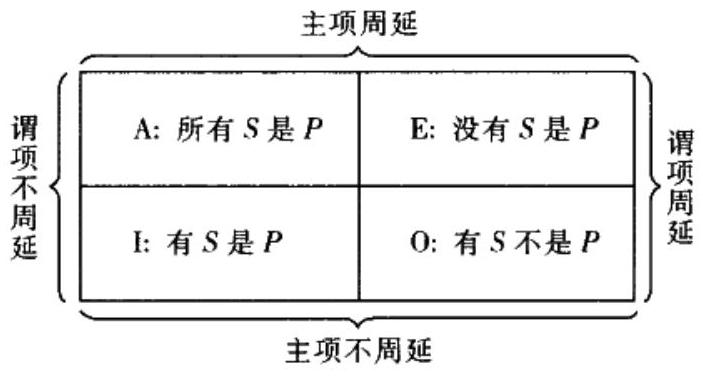
\includegraphics[width=\textwidth]{images/2025_05_15_6a28331d5e7c993ad07ag-234.jpg}

图 5-2 周延性总结
\end{center}

\begin{center}
\fbox{\parbox{0.95\textwidth}{
\textbf{本节要点}
\begin{itemize}
\item \textbf{质}:命题或肯定或否定,决定谓项的周延性
  \begin{itemize}
  \item 肯定命题(A和I):谓项不周延
  \item 否定命题(E和O):谓项周延
  \end{itemize}
\item \textbf{量}:命题或全称或特称,决定主项的周延性
  \begin{itemize}
  \item 全称命题(A和E):主项周延
  \item 特称命题(I和O):主项不周延
  \end{itemize}
\item \textbf{标准式直言命题的一般模式}:量项(主项)联项(谓项)
\item \textbf{周延性}:一个词项是周延的,当且仅当命题述及该词项所指称的类的全部元素
\item 四种标准式命题的周延性:
  \begin{itemize}
  \item A命题:主项周延,谓项不周延
  \item E命题:主项周延,谓项周延
  \item I命题:主项不周延,谓项不周延
  \item O命题:主项不周延,谓项周延
  \end{itemize}
\end{itemize}
}}
\end{center} 
\section{传统对当方阵}

\begin{quotation}
对当方阵是传统逻辑中分析直言命题之间关系的重要工具,包含矛盾关系、反对关系、下反对关系和差等关系四种基本关系类型。这些关系为直接推论提供了逻辑基础,帮助我们从一个命题的真假推断出相关命题的真假情况。
\end{quotation}

具有相同主项和相同谓项的标准式直言命题,可能在量上有所不同,或者在质上有所不同,也可能在质与量上都不同。先前的逻辑学家称之为\textbf{对当关系}(opposition),各种对当关系之间有很重要的真值联系。

\subsection{矛盾关系(Contradictories)}
两个命题之间具有\textbf{矛盾关系},如果一个是另一个的拒斥(denial)或否定(negation),也就是说,它们既不能同真也不能同假。显而易见,如果两个标准的直言命题的主项相同、谓项也相同,而质、量都不同,那么,它们就是矛盾的。例如 A 和 O 就是这样的,比如:

\begin{quote}
所有法官都是律师。

与

有法官不是律师。
\end{quote}

这两个命题的质与量都是对立的,显然它们是矛盾的。其中之一为真时,另一个恰恰为假。

同理,E 和 I 也是这样:

\begin{quote}
没有政客是理想主义者。

与

有些政客是理想主义者。
\end{quote}

这两个命题的质与量都是对立的,因而它们是矛盾的。用公式表示就是:"所有 $S$ 是 $P$"的矛盾命题是"有 $S$ 不是 $P$",而"没有 $S$ 是 $P$"的矛盾命题是"有 $S$ 是 $P$ ";A 和 O 互为矛盾,E 和 I 互为矛盾。

\subsection{反对关系(Contraries)}
两个命题之间具有\textbf{反对关系},如果它们不能同时为真,也就是说,可以由一个的真推出另一个的假。例如,"得克萨斯队将在比赛中战胜俄克拉何马队"与"俄克拉何马队将在比赛中战胜得克萨斯队"就是反对的;如果两个命题中的一个(当然指的是在同一场比赛中)是真的,那么另一个必定为假。但它们不是矛盾的,因为如果他们打成平手,两个命题就同时为假。具有反对关系的两个命题,不能同时为真,但可以同时为假。

传统逻辑或曰亚里士多德逻辑认为,如果两个直言命题都是全称的,其主、谓项分别相同而质不同,那么它们就是互相反对的。\cite{kneale1962} A 命题和相应的 E命题不能同时为真,却可以同时为假,所以它们之间是反对关系,例如"所有诗人都是懒汉"与"没有诗人是濑汉"。

如果 A 命题或者 E 命题是必然真的一一即在逻辑上或数学上为真一一那么,说它们是互相反对的就是不正确的。例如,"所有三角形都是四边形"与"没有三角形是四边形"。如果一个命题是必然真的一一不可能为假的一一那么,它就没有反对命题,因为互相反对的命题可以同假。我们把既非必然真也非必然假的命题称为\textbf{偶真的}(contingent)。如果一个 A 命题和一个 E 命题都是偶真的,并且它们有相同的主项和相同的谓项,那么,说它们是反对的就是正确的。本章其他部分的讨论都假定 A和 E 是偶真的。

\subsection{下反对关系(Subcontraries)}
两个命题之间具有\textbf{下反对关系},如果它们不能同假,但可以同真。传统上认为,如果两个直言命题都是特称的,其主、谓项分别相同而质不同,那么它们之间是下反对关系。也就是肯定了 I 和 O 命题,可以同真但不可同假,如:

\begin{quote}
有钻石是珍贵的石头。

有钻石不是珍贵的石头。
\end{quote}

必定是下反对的。

如果 I 和 O 必然为假,那么,说它们是下反对的就不正确。例如"有正方形是圆"与"有正方形不是圆"。如果一个命题必然为假——也就是说,不可能为真一一那么它就不会有下反对的对立面。因为,两个互为下反对的命题是可以同真的。当然,如果 I 和 O 都是偶真的,就可以同真。与反对关系一样,本章其他部分的讨论亦假定 I 和 O 都是偶真的。

\subsection{差等关系(Subalternation)}
如果两个命题有相同的主项和相同的谓项,并且它们的质相同(即都是肯定的或者都是否定的),但量不同(即一个为全称,另一个为特称),那么,它们之间的关系就是\textbf{差等关系}。例如,A 命题:

\begin{quote}
所有蜘蛛都是八脚动物。
\end{quote}

有一个相应的 I 命题:

\begin{quote}
有蜘蛛是八脚动物。
\end{quote}

而 E 命题:

\begin{quote}
没有鲸是鱼。
\end{quote}

也有一个相应的 O 命题:

\begin{quote}
有鲸不是鱼。
\end{quote}

此前用于说明命题间对当关系的例子都有"对立"(disagreement)的含义。但这里使用的"对当关系"是个专业术语,也适用于并不存在"对立"含义的情况。在上面的例子中,A 命题和相应的 I 命题之间不"对立",E命题和 O 命题之间也不"对立",但它们却都具有一种特殊的"对当关系"。全称命题与相应的特称命题之间的对当关系叫做差等关系。在一对相应的命题中,比如刚才给出的两对,全称命题叫做\textbf{上位式},特称命题叫做\textbf{下位式}。

传统上认为,在差等关系中,上位的真蕴涵下位的真。举例来说,从全称肯定命题"所有鸟是有羽毛的"可以得出特称肯定命题"有鸟是有羽毛的";而从全称否定命题"没有鲸是鱼"可以得出特称否定命题"有鲸不是鱼"。但下位并不蕴涵上位。从特称肯定命题"有动物是猫"不能得出全称肯定命题"所有动物是猫"。同样,从特称否定命题"有动物不是猫"当然也不能推出"没有动物是猫"的结论。

\subsection{对当方阵}
命题之间这四种对当关系——矛盾关系、反对关系、下反对关系以及上位与下位之间的差等关系——可以用一个重要且广为应用的图示来表示,称为\textbf{对当方阵},见图 5-1。

\begin{center}
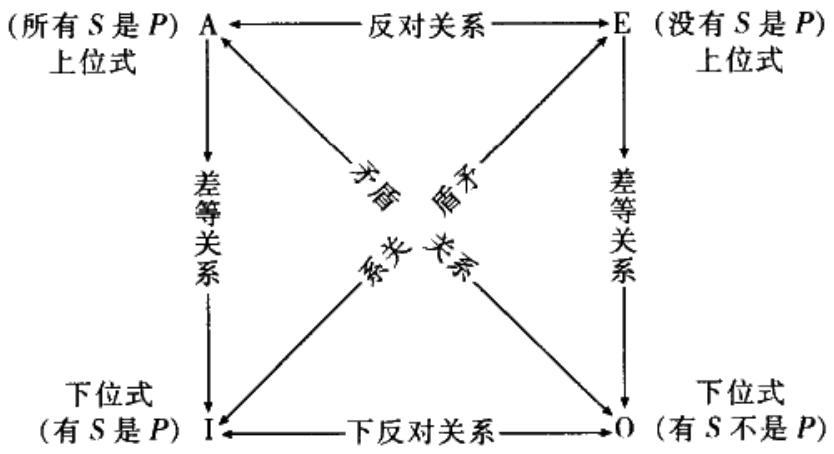
\includegraphics[width=\textwidth]{images/2025_05_15_6a28331d5e7c993ad07ag-238.jpg}

图 5-1 对当方阵
\end{center}

展示在对当方阵中的关系,为把握论证的一些基本形式的有效性提供了一个逻辑基础。如果我们按照惯例将论证分为\textbf{直接推论}和\textbf{间接推论},那就更容易理解了。

任何论证都是从一个或多个前提得出一个结论。包括一个以上前提的推论叫做间接推论,例如三段论,其结论就是从第一个前提经由第二个前提为中介得出的。而如果从唯一的前提出发,不经过任何中介推得结论,这样的推论叫做直接推论。容易见得,许多非常有用的直接推论,可从传统对当方阵所包含的知识中获得。

下面看一些例子。如果以 A 命题为前提,根据对当方阵,可以有效地推出相应的(即主、谓项分别相同的)O命题为假。从同样的前提也可以有效地推出相应的 I 命题为真。当然,从 I 命题的真不能推出相应的 A命题为真,但可以推出其矛盾命题 E 为假。以对当方阵为基础,还可以得到许多这样的直接推论。给定任一标准式直言命题的真假情况,就可以直接得到其他某个或者所有其他相应命题的真假情况。基于对当方阵的直接推论可以列表如下:

\begin{enumerate}
\item 如果 A 真,那么, E 假、 I 真、 O 假;
\item 如果 E 真,那么, A 假、 I 假、O 真;
\item 如果 I 真,那么,E 假,A、O 真假不定;
\item 如果 O 真,那么,A 假,E、I 真假不定;
\item 如果 A 假,那么,O 真,E、I 真假不定;
\item 如果 E 假,那么, I 真, A 、O 真假不定;
\item 如果 I 假,那么, A 假、 E 真、O 真;
\item 如果 O 假,那么, A 真、 E 假、 I 真。
\end{enumerate}



\begin{center}
\fbox{\parbox{0.95\textwidth}{
\textbf{本节要点}
\begin{itemize}
\item 对当方阵展示了四种基本的命题关系:矛盾关系、反对关系、下反对关系和差等关系
\item 矛盾关系:两命题不能同真也不能同假(A与O, E与I)
\item 反对关系:两命题不能同真但可以同假(A与E)
\item 下反对关系:两命题不能同假但可以同真(I与O)
\item 差等关系:上位命题的真蕴涵下位命题的真,但下位的真不蕴涵上位的真(A与I, E与O)
\item 对当方阵为直接推论提供了重要的逻辑基础
\end{itemize}
}}
\end{center} 
\section*{5.5 其他直接推论}
除了基于对当关系的直接推论,还有另外一些直接推论,本节我们来讨论其中的三种。

\section*{A.换位法(Conversion)}
第一种叫做换位法,它是一种仅仅通过交换命题中主、谓项的位置而进行的推论。对于 E 命题和 I 命题来说,换位法肯定是有效的。很显然,若断言"没有人是天使",也就可以断言"没有天使是人"。这两个命题可以通过换位法进行有效的互推。同样显然的是,"有作家是妇女"与"有妇女是作家"在逻辑上也是等价的,可以通过换位从其中一个有效地推出另一个。一个标准式直言命题叫做另一个的换位命题,如果它是通过交换另一个命题的主、谓项的位置而得到的。例如,"没有理想主义者是政治家"是"没有政治家是理想主义者"的换位命题,它们可以通过换位有效地互推。换位法直接推论中的前提叫做被换位命题(convertend),结论叫做换位命题(converse)。

请注意,从被换位 A 命题不能普通有效地推出换位 A 命题。比如,已知"所有狗是动物",当然不能有效地推出它的换位命题"所有动物是狗",因为被换位命题为真,而换位命题为假。传统逻辑自然也认识到这一点,但它认为对于 A 命题进行某种类似换位的推论可以是有效的。如 5.4 节表明,依据对当方阵,从 A 命题(所有 $S$ 是 $P$ )可以有效地推出其相应的下位 I命题(有 $S$ 是 $P$ )。A 命题说的是 $S$ 类中全部元素的情况,而 I 命题则限制为只述及 $S$ 类中的部分元素的情况。我们已经知道 I 命题是可以有效换位的。

这样,给定一个 A 命题(所有 $S$ 是 $P$ ),就可以根据差等关系,有效地得到相应的下位命题(有 $S$ 是 $P$ ),而下位命题(有 $S$ 是 $P$ )又可以进行有效换位,因此,通过差等关系和换位法的结合,从所有 $\boldsymbol{S}$ 都是 $\boldsymbol{P}$ 就可有效地推出有 $\boldsymbol{P}$ 是 $\boldsymbol{S}$ 。这种推论称为限制换位(或"偶然换位"[conver-\\
sion per accidens]),即交换主谓项的位置,同时将命题的量由全称改为特称。因此,按照传统逻辑的认识,"所有狗都是动物"可以有效地推出"有动物是狗",这个推论就是"限制换位"。下一节将进一步探讨这个问题。

请注意,作为限制换位结论的换位命题与原来的 A 命题并不等价,原因在于限制换位需要改变命题的量,把全称改为特称。因此,限制换位的结果不是一个 A 命题而是 I 命题,它不可能与被换位命题有同样的意义,从而不可能在逻辑上等价。但 E 命题的换位命题仍是一个 E 命题, I命题的换位命题仍是一个 I 命题,在这样的情况下,被换位命题与换位命题有同样的量,并且在逻辑上是等价的。

最后需要注意的是, O 命题的换位一般是无效的。 O 命题"有动物不是狗"很明显是真的,但它的换位命题"有狗不是动物"显然是假的。O命题与其换位命题并不等价。

一命题的换位命题总与原命题词项相同(只是位置互换),并且质也相同。下表是对传统换位推论的完整描述:

\section*{B.换质法(Obversion)}
接下来讨论的直接推论类型叫做换质法。在解说之前,我们先简要回顾一下"类"这个概念,并由此引人一些新的概念,以便更容易讨论换质法。一个类就是具有某种共同属性的所有对象的汇集。这种共同属性叫做 "类的定义特征"(class-defining characteristic)。举例来说,所有人的类就是所有具有"是人"这个特征的事物的集合,属性"是人"就是这个类的定义特征。类的定义特征不一定是"简单"的属性,任何一个属性都可以确定一个类。比如"左撒子、有红头发并且是学生"这个复杂属性就确定了一个类——所有是左撇子、有红头发的学生的类。

所有的类都有一个相应的补类(complementary class),或简称补 (complement),即不属于原来的类的所有东西的汇集。比如,所有人的类

的补就是所有不是人的东西组成的类。该类的定义特征是不是人这样一个 (否定的)属性。所有人的类的补包括除人之外的所有东西:鞋子、轮船、封蜡和大白菜等等——但不包括国王,因为国王是人。把所有人的类的补称为"非人的类"更简洁一些,词项 $S$ 所指称的类的补则由词项非 $S$ 指称,因而可以说词项非 $S$ 就是词项 $S$ 的补。 ${ }^{[3]}$

我们在两种意义上使用"补"这个词:一是类意义上的补,二是词项的补。尽管两者有所不同,但却是密切联系着的。一个词项是另一词项的词项补,仅当第一个词项指称第二个词项所指称的类的补。应当说明的是,正如一个类是其(类)补的补一样,一个词项也是其(词项)补的补。其中用到了"双重否定"法则,这样就可以省去许多用做前缀的 "非"字。例如,如果把词项"选举人"的补写做"非选举人",而"非选举人"的补就简记为"选举人",而不是"非非选举人"。必须注意不要把反对词项当做互补词项,比如将"懦夫"等同于"非英雄"。没有既是懦夫又是英雄的人,但并非每个人--当然更不是任何东西--都必须或者是懦夫或者是英雄,所以词项"懦夫"与"英雄"之间是反对关系。再比如 "胜者"的补不是"败者"而是"非胜者",因为并非所有东西——或者说所有人——必须或是胜者或是败者。但每个东西必定或是胜者或是非胜者。

了解了词项补的含义,换质法就比较容易描述了。在换质法中,主项保持不变,被换质命题的量也不需改变。对一个命题进行换质,就是改变其质,并用谓项的补替换原来的谓项。例如下面这个 A 命题:

所有居民都是选举人。

换质后成为一个 E 命题:

没有居民是非选举人。

泉然,这样两个命题在逻辑上是等价的,因此从一个可以有效地推出另一个。换质法应用到任何标准式直言命题,都是有效的直接推论。例如,下面的 E 命题:

换质后得到一个等值的 A 命题:

所有仲裁人都是不偏心的。

同样的,I 命题:

有金属是导体。

换质后得到一个 O 命题:

有金属不是非导体。

最后,()命题:

有国家不是好战的。

换质后得到一个 I 命题:

有国家是不好战的。

换质法直接推论中的前提叫做被换质命题(obvertend),结论叫做换质命题(obverse)。所有标准式直言命题与其换质命题在逻辑上都是等价的,所以,对任何一个标准式直言命题而言,换质法都是有效的。要得到一个命题的换质命题,不需改变原命题的量和主项,而是要改变它的质,并用谓项的补替换原来的谓项。下表对传统上的换质推理进行了全面的刻画:

\begin{center}
\begin{tabular}{|l|l|}
\hline
\multicolumn{2}{|c|}{换质表} \\
\hline
被换质命题 & 换质命题 \\
\hline
A:所有 $S$ 是 $P$ & E :没有 $S$ 是非 $P$ \\
\hline
E :没有 S 是 $P$ & A:所有 $S$ 是非 $P$ \\
\hline
I:有 $S$ 是 $P$ & O :有 $S$ 不是非 $P$ \\
\hline
O :有 $S$ 不是 $P$ & I :有 $S$ 是非 $P$ \\
\hline
\end{tabular}
\end{center}

\section*{C.换质位法(Contraposition)}
讨论第三种直接推论并不需要引人新的原理,从一定意义上讲,这种方法可以还原为前面两种推论。对给定的命题进行换质位,就是将主项换为原命题谓项的补,并将其谓项换为原命题主项的补。例如,A命题:

所有会员都是选举人。

换质位后是 A 命题:

所有非选举人都是非会员。

容易见得,以上两个命题在逻辑上是等价的。对 A 命题进行换质位是有效的直接推论形式。对 A 命题首先换质,再换位,然后再换质,于是就从最初的"所有 $S$ 是 $P$"转化为"所有非 $P$ 是非 $S$"。因此,对任何一个 A 命题进行换质位,都是将原命题先换质,再换位,然后再换质。

换质位法用于 A 命题是最有用的,用于 O 命题也是有效的直接推论形式。例如对于 $O$ 命题:

有学生不是理想主义者。

换质位后得到一个有点绕口的 O 命题:

有非理想主义者不是非学生。

它与第一个命题在逻辑上是等价的。如果每次只转化一步,即先换质,再换位,再换质,那么就可以显示出其逻辑等价性。可把其中的推论用公式表示为:从"有 $S$ 不是 $P$"换质得"有 $S$ 是非 $P$",再换位得"有非 $P$ 是 $S$",继续换质得"有非 $P$ 不是非 $S$"(换质位命题)。

一般说来,换质位法对于 I 命题无效。用下面这个真的 I 命题可以证明这一点:

有公民是非议员。

换质位后得到一个假命题:

有议员是非公民。

其无效的原因在于对 I 命题进行换质位,就要对 I 命题先换质,再换位,然后再换质。I命题"有 $S$ 是 $P$"换质后得 O 命题"有 $S$ 不是非 $P$",而后者一般不能有效换位。

E 命题"没有 $S$ 是 $P$"的换质位命题是"没有非 $P$ 是非 $S$",这也不是从原命题有效地得出的,下面的例子可以说明这一点, E 命题:

没有摔跤运动员是体弱的人。

其为真,但完全换质位命题却是假的:

没有非体弱的人是非挥跤运动员。

为了得到其换质位命题,我们对 E 命题先进行换质,再换位,然后再换质,就可以找到无效的原因。 E 命题"没有 $S$ 是 $P$"换质后得 A 命题 "所有 $S$ 是非 $P$"。一般说来,A命题不能有效地换位,除非进行限制换位。于是,通过限制换位得"有非 $P$ 是 $S$",再换质得"有非 $P$ 不是非 $S$",我们称之为"限制换质位"。下一节我们将进一步讨论这个问题。

请注意,通过限制性换质位法,我们可从一个 E 命题推得一个 O 命题——一即从"没有 $S$ 是 $P$"推出"有非 $P$ 不是非 $S$"——与限制换位有同样的特点。由于从全称命题只能推特称命题,结果得到的换质位命题与原命题意义不同,与作为原命题的 E 命题逻辑上不等价。而 A 命题的换质位命题仍是 A 命题, O 命题的换质位命题仍是 O 命题,在这两种情况下,换质位命题与其前提是等值的。

因此,换质位法只对 A 命题和 O 命题是有效的,对 I 命题是无效的,对 E 命题进行限制换质位才是有效的。也可以用一个图表来完整刻画这种

\begin{center}
\begin{tabular}{|l|l|}
\hline
\multicolumn{2}{|c|}{换质位表} \\
\hline
前提 & 完全换质位命题 \\
\hline
A:所有 $S$ 是 $P$ & A:所有非 $P$ 是非 $S$ \\
\hline
E :没有 $S$ 是 $P$ & O :有非 $P$ 不是非 $S$(限制) \\
\hline
I:有 $S$ 是 $P$ & (换质位无效) \\
\hline
O :有 $S$ 不是 $P$ & O :有非 $P$ 不是非 $S$ \\
\hline
\end{tabular}
\end{center}

还有一些其他类型的直接推论,也都有各自的分类与特定名称,但并不需要引人新原理,我们在此就不再讨论了。

若要解决关于命题之间关系的某些问题,最好的方法就是研究从其中一个可以推得另一个的各种直接推论。例如,假定命题"所有外科医生都是内科医生"为真,是否可以推知"没有非外科医生是非内科医生"的真假情况?在此可以给出一个有用的方法,就是尽可能从给定命题推出多个有效结论,来看要考察的命题——或其矛盾命题和反对命题——是否能从为真的原命题有效地推出。上面的例子中,已知"所有 $S$ 是 $P$",我们可以有效地推出其换质位命题"所有非 $P$ 是非 $S$",再限制换位得"有非 $S$是非 $P$"——按照传统逻辑,它是已知命题的有效结论,因此是真的。根据逻辑方阵,它与被考察的命题"没有非 $S$ 是非 $P$"为矛盾关系,因此被考察的命题就是假的。

如 1.9 节所指出的,一个有效推理,如果前提为真,其结论必然为真。但如果前提为假,结论却可能为真。我们立即会联想到限制换位、限制换质位以及差等关系推理,它们正是后面一种情况的例子。例如,从假前提"所有动物是猫",根据差等关系推理,可以推出"有动物是猫"这样一个真结论。而假前提"所有父母都是学者"限制换位后也可以得到一个真结论"有学者是父母"。因此,如果已知一个命题为假,那么另一个(与之多少有些关系的)命题的真假情况就成了问题。比较好的方法是,从已知命题的矛盾命题或被考察命题本身着手。因为一个假命题的矛盾命题必然为真,所有从后者开始的有效推理也必然是真命题。而如果从被考察命题能够推出已知为假的命题,那么它本身也必然是假的。

\begin{center}
\begin{tabular}{|l|l|}
\hline
\multicolumn{2}{|c|}{换位法、换质法、完全换质位法} \\
\hline
\multicolumn{2}{|c|}{换位法} \\
\hline
被换位命题 & 换位命题 \\
\hline
A:所有 $S$ 是 $P$ & I:有 $P$ 是 $S$ \\
\hline
E :没有 S 是 $P$ & E :没有 $P$ 是 $S$ \\
\hline
I:有 $S$ 是 $P$ & I:有 $P$ 是 $S$ \\
\hline
O :有 $S$ 不是 $P$ & (换位无效) \\
\hline
\multicolumn{2}{|c|}{换质法} \\
\hline
被换质命题 & 换质命题 \\
\hline
A:所有 $S$ 是 $P$ & E :没有 $S$ 是非 $P$ \\
\hline
E :没有 $S$ 是 $P$ & A:所有 $S$ 是非 $P$ \\
\hline
I:有 $S$ 是 $P$ & O:有 $S$ 不是非 $P$ \\
\hline
O :有 $S$ 不是 $P$ & I:有 $S$ 是非 $P$ \\
\hline
\multicolumn{2}{|c|}{换质位法} \\
\hline
前提 & 完全换质位命题 \\
\hline
A:所有 $S$ 是 $P$ & A:所有非 $P$ 是非 $S$ \\
\hline
E :没有 $S$ 是 $P$ & O :有非 $P$ 不是非 $S$(限制) \\
\hline
I:有 $S$ 是 $P$ & (换质位无效) \\
\hline
O :有 $S$ 不是 $P$ & O :有非 $P$ 不是非 $S$ \\
\hline
\end{tabular}
\end{center}
\footnotetext{(3)我们有时用类的"相对补"(relative complement)来进行推论,即它的补包含在另外一个类中。比如:"我的孩子"这个类有一个子类"我的女儿",后者的补是另一个子类"我的不是女儿的孩子",即"我的儿子"的类。但换质法以及其他直接推论通常建基于类的绝对补之上,正如上面所定义的那样。} 
\section*{5.6 存在含义与直言命题的解释}
进一步分析和评估由直言命题构成的论证,需要对它们进行图示与符号化。但是,把 A、E、I、O 命题符号化,必定会遇到而且必须解决一个深层的逻辑问题——一个上千年长期争论的问题。本节我们就来说明这个问题,同时提供一种解决方案。以此为基础,也可以对三段论做出融贯的分析。

首先要说明的是,这并不是一个简单的问题。但只要我们弄清如下关于直言命题的解释(称为布尔解释[Boolean interpretation]),则后面关于三段论的分析并不需要对有关争议的深度把握。如果能掌握本节最后所总结的讨论结果,就可以顺利越过此前的复杂讨论。

要理解这个结果,必须弄清有些命题有存在含义(existential im- port),有些则没有。如果说出一个命题就肯定了某种对象的存在,那么就说这个命题有存在含义。

为什么初学逻辑就要关心这个看上去很深奥的问题呢?这是因为,特定论证中所用的命题中是否有存在含义,将直接影响到该论证中推理的正确性。对直言命题必须有一个清晰、融贯的解释,以便能确定什么东西可以从它们正确地推出,同时避免错误推论。

先看 I 命题和 O 命题,它们肯定有存在含义。例如 I 命题"有士兵是英雄"说的是至少存在一个是英雄的士兵。而 O 命题"有狗不是同伴"说的是至少存在一个不是同伴的狗。特称命题 I 和 O,一般说来,确实断定了主项(例句中的士兵和狗)指称的类不为空——士兵的类和狗的类(如果给出的例子为真的话)中至少有一个元素。 ${ }^{[4]}$

如果确实如此,即如果 I 和 O 命题有存在含义(没人会否认),会有

什么问题呢?问题在于这种状况的后果令人十分不安。先前我们已经说过,通过差等关系推论,I 命题可以从相应的 A 命题有效地推出,也就是说,从"所有蜘蛛都是八脚动物"可以有效地推出"有蜘蛛是八脚动物"。同样,我们说 O 命题可以有效地从 E 命题推得。但如果 I 和 O 命题有存在含义,而它们分别是从 A 和 E 命题得到的,那么 A 和 E 命题必定也要有存在含义。因为一个有存在含义的命题不可能有效地从另一个没有同样含义的命题得到。 ${ }^{[5]}$

这种结果造成了一个严重的问题。我们知道在传统逻辑方阵中,A 和 O 命题是矛盾关系。"所有丹麦人都说英语"与"有丹麦人不说英语"是互为矛盾的。具有矛盾关系的命题不可同真,因为其中必有一假。两者也不可同假,因为其中必有一真。但如果像上文总结的那样,对应的 A 和 O命题确实有存在含义的话,那么,两个矛盾命题就可能同时为假!举例来说,A命题"所有火星人都是金发碧眼的"与其对应的 O 命题"有火星人不是金发碧眼的"互为矛盾,如果它们都有存在含义的话——即我们要把它们看做都断言存在火星人的话——那么,如果火星上没有居民则两个命题都是假的。我们当然知道火星上没有人,火星人的类是空类,据此上述例子中给出的两个命题都是假的。而如果两者都是假的,它们就不可能是矛盾关系!

由此看来,传统对当方阵是有不妥之处的。假如它所说 A 和 E 命题有效地蕴涵相应的 I 和 O 命题是正确的话,那么,它断言 A 和 O 命题之间有矛盾关系就不正确了,同样,认为 I 和 O 命题为下反对关系也是不正确的。

那么我们该怎么办呢?传统逻辑方阵还能否加以挽救?挽救是可以的,但代价很高。我们可以引入预设(presupposition)概念来恢复逻辑方阵的地位。我们早已注意到(见 4.3 节),对于一些复杂问语,只有已经预设了先行问题的答案,才能适当地回答"是"或"否"。只有预设了你偷过钱是真的,才能用"是"或"否"来回答"你把偷来的钱花光了吗"这样的问题,否则是不合理的。现在,为挽救传统逻辑方阵,我们可以主张所有直言命题,即四种标准式命题 A、E、I、O——都预设(在上述含义下)它们涉及的类均不为空,即都有元素。也就是说,要使命题的真假情况以及它们之间的逻辑关系都成立并可以得到合理的解答(在这种解释下),就必须预设它们绝不涉及空类。这样,就可以保留传统对当方

阵中构建的各种关系: A 与 E 仍是反对关系, I 与 O 仍是下反对关系, A与 $\mathrm{O} 、 \mathrm{E}$ 与 I 仍是矛盾关系。然而,为了保证这个结果,必须诉诸其全面存在预设(blanket presupposition),即预设全部词项指称的类(及其补类)都有元素,都不为空。 ${ }^{[6]}$

那么,我们为什么不能就此罢休呢?存在预设对于挽救亚里士多德型逻辑既是必要的也是充分的。而且,预设在很多情况下与现代语言的日常用法是一致的。如果有人告诉你说"桶里的苹果都是甜的",而你向桶里一看,却什么都没有,那你会怎么说?你可能不会说刚才的话是假的或真的,而是指出这里没有苹果。你会解释说,说话人犯了一个错误,即当时的存在预设(桶里有苹果)是假的。事实上,这种纠正已经表明我们理解并基本接受了日常语言中的预设。

然而不幸的是,用来挽救逻辑方阵的这种全面预设却要付出一个过重的代价,是我们不能接受的。我们有充分的理由不这样做,在此列举三条理由。

首先,引人预设确实能够保留 A、E、I 和 O 之间的对当关系,但却付出了不能刻画某些我们需要的断言的代价,即不能再刻画那些否定有元素存在的命题了。而这样的否定有时非常重要,是必须明确的。

其次,即使是日常语言的用法,也并不完全与全面存在预设一致,有时我们说的话并不假定所谈的类中有元素。例如,你说"所有非法侵入者都要被起诉",这句话根本不预设非法侵人者的类中已经有元素,相反,你这样说正是为了保证这个类维持空类。

再次,在科学界及其他理论界,我们通常希望进行没有任何存在预设的推理。例如牛顿第一运动定律断定的是不受任何外力作用的物体必然保持静止状态或匀速直线运动。这种定律可以是真的,而物理学家表述它并为它辩护的时候,并没有预设不受任何外力作用的物体存在。

这些问题的存在使得上述全面存在预设不能为现代逻辑学家所接受。我们应当放弃曾长期被认为是正确的亚里士多德型解释,而采用关于直言命题的现代解释。

直言命题的现代解释不再假定我们言说的类中必定有元素。拒绝这种假定的解释称为布尔解释。英国逻辑学家、数学家乔治•布尔(George Boole,1815-1864)是现代符号逻辑奠基人之一,这种新的解释就是以

他的名字命名的。 ${ }^{[7]}$\\
在本书以下部分,我们均采纳关于直言命题的布尔解释。现在我们就来阐明这种解释:

1.在某些方面,传统解释仍然成立。 $\mathbf{I}$ 和 $\mathbf{O}$ 命题在布尔解释中仍然有存在含义。所以,如果 $S$ 类为空,那么,命题"有 $S$ 是 $P$"为假,命题 "有 $S$ 不是 $P$"也为假。

2.全称命题 $\mathbf{A}$ 和 $\mathbf{E}$ 与特称命题 $\mathbf{O}$ 和 $\mathbf{I}$ 之间的矛盾关系也保持为真。也就是说,命题"所有人是会死的"与"有人不是会死的"互为矛盾,而命题"没有神灵是会死的"与"有神灵是会死的"亦互为矛盾。

3.在布尔解释中上述关系是完全融贯的,这是因为,全称命题被解释为没有存在含义。因此,即使 $S$ 类为空,命题"所有 $S$ 是 $P$"仍可以为真,"没有 $S$ 是 $P$"也可以为真。例如,即使独角兽不存在,"所有独角兽是有角的"与"没有独角兽是有翅膀的"都可以为真。而如果不存在独角兽,I 命题"有独角兽是有角的"就是假的,O 命题"有独角兽不是有翅膀的"同样为假。

4.在日常话语中,有时我们说出一个全称命题,确实假定了某事物的存在。当然,布尔解释也允许有这种表述,但要求用两个命题来表述,一个是有存在含义的特称命题,加之一个没有存在含义的全称命题。

5.采纳布尔解释会带来一些重要变化。相应的 $\mathbf{A 、 E}$ 命题可以同真,因此它们之间不再是反对关系。这似乎有点怪异,在后面 10.2 和 10.3 部分将给出详细的说明。现在弄清如下这点就足够了:在布尔解释中,"所有独角兽是有翅膀的"断言的是"如果有独角兽,那么,它是有翅膀的"。而"没有独角兽是有翅膀的"断定的是"如果有独角兽,那么,它是没有翅膀的"。如果确实不存在独角兽,这两个"如果……那么……"型的命题都可以为真。

6.类似的,在布尔解释中,因为 I 和 O 命题确实有存在含义。所以,如果主项指称的类为空,相应的 I 和 O 命题都是假的,因此相应的 I 和 O命题之间也不再是下反对关系。

7.在布尔解释中,差等关系——从 A 命题推出相应的 I 命题,从 E命题推出相应的 O 命题——不是普遍有效的。从一个没有存在含义的命题

当然不能得出一个有存在含义的命题。\\
8.布尔解释保留了一些直接推理: $\mathbf{E}$ 命题和 $\mathbf{I}$ 命题的换位推理, $\mathbf{A}$ 命题和 O 命题的换质位推理,所有命题的换质推理。但限制换位、限制换质位推理不再有效。

9.在布尔解释下,遌辑方阵转变为如下情形:方阵周边的关系不再成立,而对角线上的矛盾关系保持不变。

简言之,现代逻辑学家否定了全面存在预设。对于一个不能明确断定其中有元素的类,我们就不能假定它有元素,否则就是错的。任何依据这种错误假定的论证都会产生存在预设谬误,简称为存在谬误。现在有了清晰的布尔解释,我们就可以构造一个有力的体系,将标准式直言命题推理符号化、图示化。
\footnotetext{(4)有极个别的例外情况,"有鬼出现在莎士比亚戏剧里"和"有希腊神在《伊利亚特》中有所描述"都是特称命题,它们当然是真的,虽然鬼和希腊神都不存在。但这是一种误导,因为这些描述本身并没有肯定或否定鬼和希腊神的存在,只是说某些特定的命题在莎士比亚的戏剧和《伊利亚特》中被肯定或否定。莎士比亚和荷马的命题不一定是真的,但他们的作品中肯定或暗含着这些命题。很明显,这只能说是例外情况,它们只出现在文学作品和神话语境中。I命题和 $O$ 命题确实是有存在含义的。}
\footnotetext{(5)有另外一种方法可以表明,传统逻辑方阵中 A 和 E 命题的存在含义必然是从 1 和 O 命题得到的。对于 A 命题,可以根据(传统逻辑中的)限制换位的有效性说明。对于 E 命题,可以根据(传统逻辑中的)限制换质位的有效性说明。得到的结果与上面是相同的:在传统選辑方阵中,如果 I 和 O 命题有存在含义,那么, A 和 E 命题必然也要有存在含义。}
\footnotetext{(6)韦伯(Phillip H.Wiebe)认为亚里士多德逻辑并不要求假定主项的补类非空。

见《亚里士多德逻辑中的存在预设》("Existential Assumptions for Aristotelian Logic", Journal of Philosophical Research 16 (1990-1991):321-328)。但亚里士多德逻辑确实要求假定:其他三个项(主项、谓项和谓项的补)所指称的类不是空的,而下面评论中的所有问题都是存在预设造成的。}
\footnotetext{(7)另一位现代符号逻辑奠基人伯特兰•罗素在著名的论文"The Existential Im- port of Propositions"(Mind,July 1905)中也阐发了这种解释。由于他是跟从 20 世纪初期的意大利伟大的数学家皮亚诺(Guiseppe Peano)学得这种解释,故称之为命题的"皮亚诺解释"。} 
\section{直言命题的符号系统与图解}

\begin{quotation}
布尔解释为直言命题提供了严谨的基础,但为了更直观地理解命题间的关系,我们需要一套符号系统和图解方法。本节介绍如何用代数符号表示直言命题,以及如何用文恩图直观展示命题的含义和相互关系,为下一章分析三段论有效性奠定基础。
\end{quotation}

直言命题的布尔解释在很大程度上以\textbf{空类}概念为基础,为方便起见,可用一个特殊的符号来表示空类。此处我们用数字"0"来代表空类。说词项$S$指称的类没有元素,就在$S$和0之间划上等号。也就是说,$S=0$表示$S$没有元素($S$的元素$s$简记为$S^{\prime}s$,说不存在$S^{\prime}s$亦即$S=0$)。

说$S$指称的类确实有元素就是否定$S$为空。断定"存在$S$′$s$"就是对$S=0$所表示的命题的否定。我们在等号上加一条斜线表示这种否定式。就是说,$S \neq 0$表示存在$S$′$s$,是对$S$为空的否定。

\subsection{直言命题的符号表示}

标准式命题都涉及两个类,所以表示它们的等式要复杂一些。两个类都分别由一个符号代表,因此可以把两个符号并排在一起,用以表示那些由同时属于两个类的元素组成的类。比如,如果$S$代表所有"讽刺作品"组成的类,$P$代表所有"诗"组成的类,那么,既是讽刺作品又是诗的东西组成的类就可以用符号$SP$表示,它代表的就是所有讽刺诗(或者说诗式讽刺作品)组成的类。两个类的共同部分或全体共同元素称为两个类的\textbf{积}(product)或\textbf{交}(intersection)。两个类的积是所有同时属于这两个类的东西组成的类。所有美国人的类与所有作家的类之积就是所有美国作家的类。(此处必须与自然语言的某些特定用法区分开来。例如,西班牙人的类与舞蹈家的类之积,不是西班牙舞蹈家的类,因为通常说的西班牙舞蹈家不是西班牙的舞蹈家,而是表演西班牙舞蹈的人。同样,抽象画家、英语课程、古董商人等等也都是这样的用法。)

使用这种新记法,我们也可以用等式和不等式将E和I命题符号化。E命题"没有$S$是$P$"说的是$S$类中没有元素是$P$类的元素,即没有东西同时属于两者。换言之,两个类的积为空,可用等式符号表示为:$SP=0$。I命题"有$S$是$P$"说的是$S$类中至少有一个元素也是$P$类的元素。这意味着$S$类和$P$类的积不空,可用不等式符号表示为:$SP \neq 0$。

对于A命题和O命题,需要引人一个表示\textbf{补类}的新方法。如5.5节所说明,一个类的补类就是所有那些不属于原类的东西的类或汇集。例如,士兵的类的补类就是所有不是士兵的东西组成的类,即非士兵的类。若用$S$代表士兵的类,则把非士兵的类记为:$\bar{S}$(读做:$S$杠),即在原来的类之上加一横杠。A命题"所有$S$是$P$"说的是$S$类的所有元素都是$P$类的元素,也就是说,没有$S$类的元素不是$P$类的元素。或者说(据换质法)"没有$S$是非$P$",像任何E命题一样,这个命题说的是,主项指称的类与谓项指称的类的积为空,可用等式符号表示为:$S\bar{P}=0$。O命题"有$S$不是$P$"换质后得逻辑等价式I命题"有$S$是非$P$",可用等式符号表示为:$S\bar{P} \neq 0$。

使用这些符号公式,就能很清晰地显示四种标准式直言命题之间的相互关系。既然A命题和O命题的符号公式分别为$S\bar{P}=0$和$S\bar{P} \neq 0$,它们显然是互为矛盾的。E命题和I命题的符号形式分别为:$SP=0$和$SP \neq 0$,显然也是互为矛盾的。布尔解释下的对当方阵可以重新表示为图5-2。

\subsection{文恩图及其应用}

命题可以用所涉及的类的图示来表达。我们用一个圆代表一个类,用指称类的词项标注它。这样$S$类可以表示为图5-3。

\begin{center}
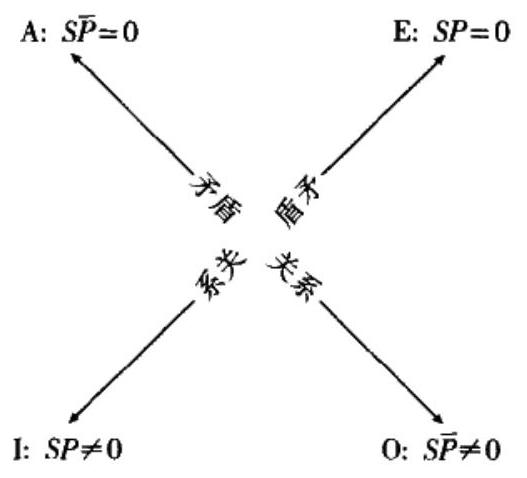
\includegraphics[width=\textwidth]{images/2025_05_15_6a28331d5e7c993ad07ag-257(2).jpg}

图5-2 布尔解释下的对当方阵
\end{center}

\begin{center}
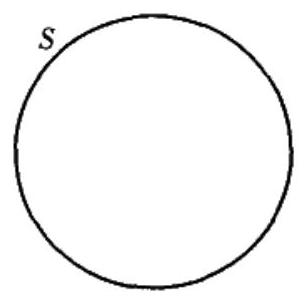
\includegraphics[width=\textwidth]{images/2025_05_15_6a28331d5e7c993ad07ag-257.jpg}

图5-3 类的图示
\end{center}

上图表示的是一个类,而不是命题。它只代表$S$类,而对这个类无所言说。要图示命题"$S$没有元素"或"不存在$S$′$s$",我们就在代表$S$的圆中加上阴影,来表示$S$中什么都没有,$S$为空类。要图示"存在$S$′$s$"这个命题,我们就在代表$S$的圆中写一个$x$,用来表示其中有东西,$S$不是空类。这样,"不存在$S$′$s$"和"存在$S$′$s$"这两个命题就可以用图5-4来表示。

\begin{center}
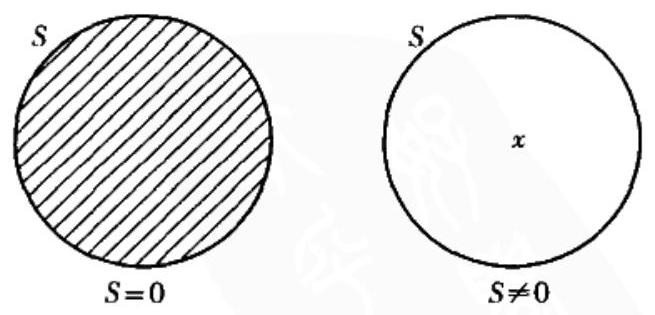
\includegraphics[width=\textwidth]{images/2025_05_15_6a28331d5e7c993ad07ag-257(1).jpg}

图5-4 空类与非空类的图示
\end{center}

实际上,表示$S$的图示也可以表示$\bar{S}$,因为圆中的部分代表的是$S$的所有元素,而圆外的部分恰好就是$\bar{S}$。

要图示标准式直言命题,一个圆不够,而需要两个圆。标准式直言命题的主、谓项分别记为$S$和$P$,而后画两个相交的圆,如图5-5。

\begin{center}
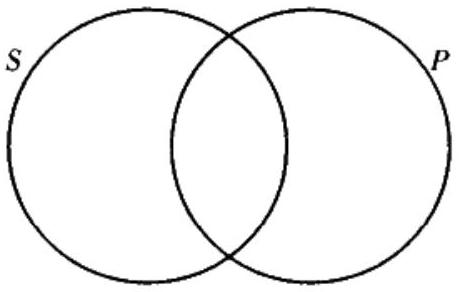
\includegraphics[width=\textwidth]{images/2025_05_15_6a28331d5e7c993ad07ag-258.jpg}

图5-5 两个类的图示
\end{center}

图示只表示出了$S$和$P$两个类,而没有表示它们形成的命题。既没有肯定也没有否定其中一个或两个类有元素。实际上,两个相交的圆表示出的类不只是$S$和$P$两个。标有$S$的圆中与$P$不重叠的部分代表的是所有不是$P$′$s$的$S$′$s$,即代表了$S$类与$\bar{P}$类的积,这一部分标记为$S\bar{P}$。两圆相交的部分代表$S$类与$P$类的积,标记为$SP$。标有$P$的圆中与$S$不重叠的部分代表的是所有不是$S$′$s$的$P$′$s$,即代表了$\bar{S}$类与$P$类的积,标记为$\bar{S}P$。最后,两个圆之外的部分,代表既不在$S$类也不在$P$类之中的东西,标记为第四个类$\overline{SP}$。加上这些标记,图5-5就成了图5-6:

\begin{center}
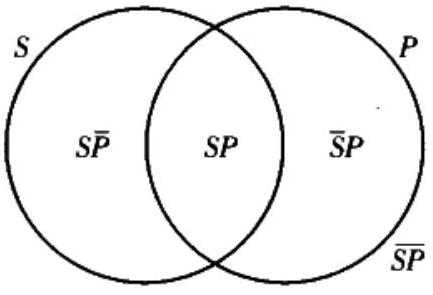
\includegraphics[width=\textwidth]{images/2025_05_15_6a28331d5e7c993ad07ag-258(1).jpg}

图5-6 文恩图中的四个类区域
\end{center}

可以用各种不同的类来解释上图。例如设西班牙人的类为$S$、画家的类为$P$,则$SP$就是两个类的积,由所有同时属于两个类的东西组成。因为$SP$的每个元素必须既是$S$类也是$P$类的元素,所以每个元素既是西班牙人又是画家。两个类的积就是西班牙画家的类,其中包括委拉斯开兹(Velásquez)和戈雅(Goya)等人。$S\bar{P}$是第一个类与第二个类之补的积,包括且只包括属于$S$类但不属于$P$类的对象,也就是不是画家的西班牙人组成的类,即所有非画家西班牙人,委拉斯开兹不在其中,戈雅也不在其中,但却包括小说家塞万提斯(Cervantes)和独裁者佛朗哥(Franco)及其他西班牙人。$\bar{S}P$是第二个类与第一个类之补的积,是那些不是西班牙人的画家组成的类,这个类包括荷兰画家伦布兰特(Rembrandt)、美国画家乔治亚•奥基夫(Georgia O'Keeffe)等。最后,$\overline{SP}$是原来两个类的补的积,包括而且只包括那些既不是西班牙人也不是画家的对象。这可是一个很大的类,包括的不只是英国海军上将和瑞士登山运动员们,还包括诸如密西西比河、珠穆朗玛峰这样的东西。如果对$S$和$P$进行这样的解释,那么,以上说的所有类都在图5-6中有所表示。

这就是\textbf{文恩图}(Venn diagram),得名于英国数学家、逻辑学家约翰•文恩(John Venn,1834-1923),他首先使用这种方法表示类和命题。像图5-6这样的带有几处标记的双圆图,所代表的仍只是类,尚不表示任何命题。整个圆或其中留做空白的部分既不表示类中有元素,也不表示没有。

但是,再加上一定条件,我们就能用文恩图来表示命题。通过给某些部分加上阴影,或者标上"$x$",就能准确地将四种标准式直言命题图示化。文恩图(带有标记的)能够全面、简明地表示命题,所以,它已经被公认为评价三段论论证的最有力、使用最广泛的方法。下面就来说明如何用文恩图表示这四种标准式命题。

A命题"所有$S$是$P$"即$S\bar{P}=0$,用文恩图图示之,可把代表$S\bar{P}$的那部分加上阴影,即表示其中没有元素。E命题"没有$S$是$P$"即$SP=0$,可把图中代表$SP$的那部分加上阴影,以示其中没有元素。I命题"有$S$是$P$"即$SP \neq 0$,可在图中$SP$类部分标上一个$x$,表示两个类的积不是空的,其中至少有一个元素。最后,O命题"有$S$不是$P$"即$S\bar{P} \neq 0$,可加一个$x$在$S\bar{P}$部分,表示其中至少有一个元素而不是空的。将以上四个图示列在一起,就能十分清晰地展现出四种命题的不同含义,见下图5-7。

我们已经用文恩图表示出"没有$S$是$P$"和"有$S$是$P$",而它们换位后分别得到一个等价命题:"没有$P$是$S$"和"有$P$是$S$",因此后面两个命题在图中也就表示出来了。要图示A命题"所有$P$是$S$"即$P\bar{S}=0$,循同样路径,可把代表$P\bar{S}$的部分加上阴影。显然,$P\bar{S}$与$\bar{S}P$是相同的,如果一下子不能明白,就回想一下是画家而非西班牙人的类,与非西班牙人中是画家的类。前一个类中的对象必定也是后一个类的对象——即所有是画家而非西班牙人的人与所有非西班牙人的画家,反之亦然。要图示命题"有$P$不是$S$"即$P\bar{S} \neq 0$,可在$P\bar{S}(=\bar{S}P)$部分加上一个$x$。图5-8展示的正是这几个命题。

\begin{center}
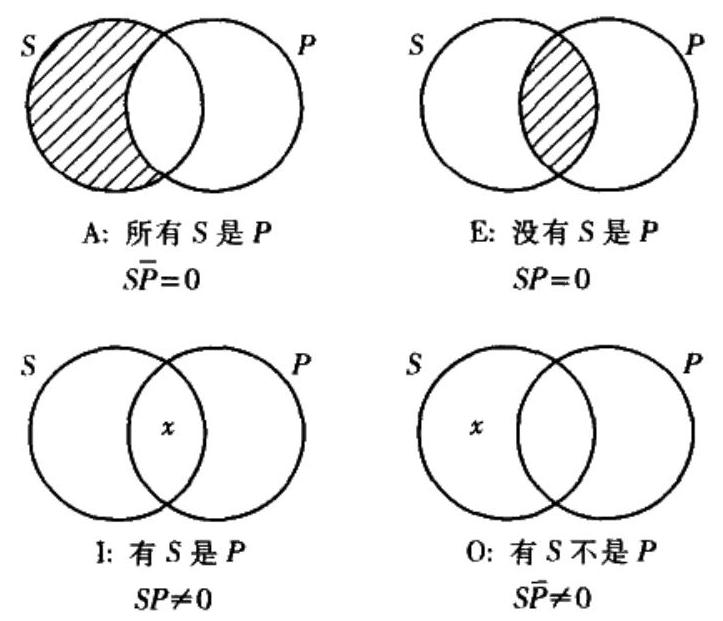
\includegraphics[width=\textwidth]{images/2025_05_15_6a28331d5e7c993ad07ag-260(1).jpg}

图5-7 四种标准式命题的文恩图
\end{center}

\begin{center}
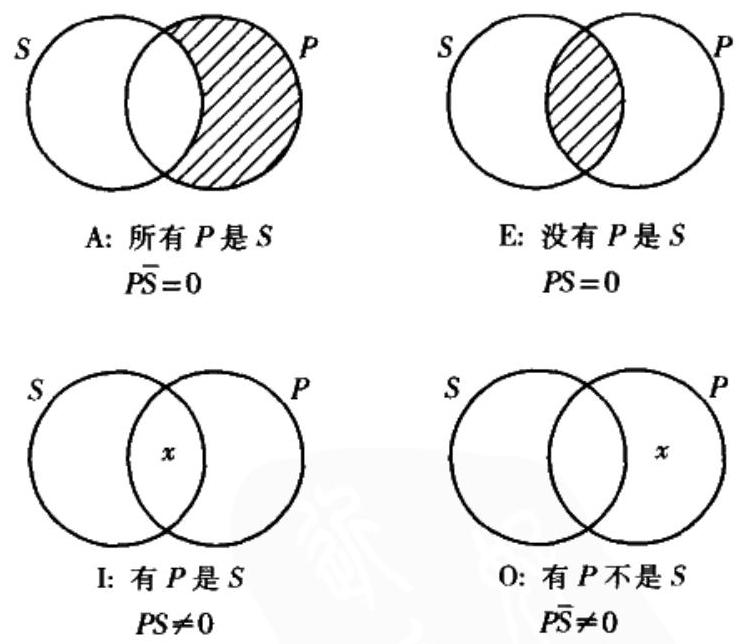
\includegraphics[width=\textwidth]{images/2025_05_15_6a28331d5e7c993ad07ag-260.jpg}

图5-8 更多命题的文恩图表示
\end{center}

双圆图的这种灵活运用,在本书下一章中起着重要作用。任给一对带有给定标记——比如$S$和$M$——的交叉圆,就能将任何一个含有$S$和$M$的标准式直言命题图示化,无论$S$和$M$出现的顺序如何。

文恩图是标准式直言命题的肖像,将空间的包含与排斥与类间非空间的包含与排斥对应起来,是一种极为清晰的记法。下一章将会看到,这也是检验直言三段论的有效性的一种最简单、最直接的方法。

\begin{center}
\fbox{\parbox{0.95\textwidth}{
\textbf{本节要点}
\begin{itemize}
\item \textbf{直言命题的符号表示}
  \begin{itemize}
  \item 空类用"0"表示,$S=0$表示类$S$没有元素
  \item 非空类用$S \neq 0$表示,表示类$S$至少有一个元素
  \item 类的积(或交)记为$SP$,表示同时属于$S$和$P$的元素组成的类
  \item 类的补记为$\bar{S}$,表示不属于类$S$的所有元素
  \item 四种标准式命题的符号表示:
    \begin{itemize}
    \item A命题:"所有$S$是$P$"$\Rightarrow$ $S\bar{P}=0$
    \item E命题:"没有$S$是$P$"$\Rightarrow$ $SP=0$
    \item I命题:"有$S$是$P$"$\Rightarrow$ $SP \neq 0$
    \item O命题:"有$S$不是$P$"$\Rightarrow$ $S\bar{P} \neq 0$
    \end{itemize}
  \end{itemize}
\item \textbf{文恩图}:用图形直观表示命题的方法
  \begin{itemize}
  \item 圆形代表类,重叠部分代表类的交
  \item 阴影表示该区域为空类
  \item 带"$x$"标记表示该区域非空
  \item 文恩图能直观展示命题间的关系,是检验三段论有效性的有力工具
  \end{itemize}
\end{itemize}
}}
\end{center} 
\chaptersummary{
\begin{logicbox}[title=第五章总览]
本章系统介绍了古典逻辑即亚里士多德型逻辑的基本构件,为理解演绎逻辑奠定了重要的理论基础。通过对直言命题的深入分析,我们建立了完整的逻辑分析框架。
\end{logicbox}

\logicemph{核心主题}:本章介绍并讨论的是\logicterm{古典逻辑}即\logicterm{亚里士多德型逻辑}的基本构件,也是\logicterm{演绎逻辑}的基本构件。

\begin{theorembox}[title=5.2 类与标准式直言命题]
\logicwarn{基础概念}:
\begin{itemize}
  \item 介绍了\logicterm{类}的概念,传统逻辑正是以类为基础建立起来的
  \item 类是具有共同属性的对象的汇集
\end{itemize}

\logicemph{四种基本命题形式}:
\begin{itemize}
  \item \logicterm{A命题}:全称肯定命题(所有S是P)
  \item \logicterm{E命题}:全称否定命题(没有S是P)
  \item \logicterm{I命题}:特称肯定命题(有S是P)
  \item \logicterm{O命题}:特称否定命题(有S不是P)
\end{itemize}

\logicwarn{重要性}:这四种形式构成了传统逻辑的基本构件。
\end{theorembox}

\begin{theorembox}[title=5.3 命题的质、量与周延性]
\logicemph{深入分析}:更加详细地考察这四种命题的内在结构。

\logicwarn{质与量}:
\begin{itemize}
  \item \logicterm{质}:肯定(A、I)和否定(E、O)
  \item \logicterm{量}:全称(A、E)和特称(I、O)
\end{itemize}

\logicemph{周延性规律}:
\begin{itemize}
  \item \logicterm{周延的项}:述及类的全部元素
  \item \logicterm{不周延的项}:只述及类的部分元素
  \item 量决定主项周延性,质决定谓项周延性
\end{itemize}
\end{theorembox}

\begin{theorembox}[title=5.4 传统对当方阵]
\logicwarn{对当关系类型}:
\begin{itemize}
  \item \logicterm{矛盾关系}:A与O、E与I(不能同真也不能同假)
  \item \logicterm{反对关系}:A与E(不能同真但可以同假)
  \item \logicterm{下反对关系}:I与O(不能同假但可以同真)
  \item \logicterm{差等关系}:A与I、E与O(上位真蕴涵下位真)
\end{itemize}

\logicemph{图示工具}:用\logicterm{对当方阵}图示了这几种关系,说明了基于传统方阵的直接推理。

\logicwarn{推理基础}:为直接推论提供了重要的逻辑基础。
\end{theorembox}

\begin{theorembox}[title=5.5 其他直接推论方法]
\logicwarn{三种推论方法}:
\begin{itemize}
  \item \logicterm{换位法}:交换主谓项位置(对E、I有效,A限制换位,O无效)
  \item \logicterm{换质法}:改变质并用谓项的补替换谓项(对所有命题有效)
  \item \logicterm{换质位法}:用谓项的补替换主项,用主项的补替换谓项(对A、O有效)
\end{itemize}

\logicemph{工具价值}:为复杂推理提供了基础工具,扩展了直接推论的范围。
\end{theorembox}

\begin{theorembox}[title=5.6 存在含义与布尔解释]
\logicwarn{核心问题}:探讨\logicterm{存在含义}问题及其对传统逻辑的影响。

\logicemph{传统解释的困境}:
\begin{itemize}
  \item 如果所有命题都有存在含义,会导致对当方阵中的矛盾关系失效
  \item 当主项指称空类时,A和O命题可能同时为假
\end{itemize}

\logicwarn{布尔解释的优势}:
\begin{itemize}
  \item 特称命题(I和O)有存在含义
  \item 全称命题(A和E)没有存在含义
  \item 保留了对角矛盾关系,避免了存在预设谬误
  \item 为现代逻辑提供了更严谨的基础
\end{itemize}
\end{theorembox}

\begin{theorembox}[title=5.7 符号系统与文恩图]
\logicwarn{符号化方法}:
\begin{itemize}
  \item A命题:$S\bar{P}=0$(所有S是P)
  \item E命题:$SP=0$(没有S是P)
  \item I命题:$SP \neq 0$(有S是P)
  \item O命题:$S\bar{P} \neq 0$(有S不是P)
\end{itemize}

\logicemph{文恩图工具}:
\begin{itemize}
  \item 用交叉的圆表示类的关系
  \item 阴影表示空类,"x"表示非空类
  \item 直观展示命题的含义和相互关系
  \item 为三段论分析提供有力工具
\end{itemize}

\logicwarn{实用价值}:为逻辑分析提供了直观的视觉工具和严谨的符号系统。
\end{theorembox}

\begin{examplebox}[title=第五章的理论意义与实践价值]
\logicwarn{理论贡献}:
\begin{itemize}
  \item \logicterm{概念体系}:建立了古典逻辑的基本构件与完整概念体系
  \item \logicterm{分类框架}:确立了A、E、I、O四种基本命题形式的分类标准
  \item \logicterm{分析工具}:提供了直接推论、对当关系、布尔解释、文恩图等多种分析方法
  \item \logicterm{逻辑基础}:为演绎推理和论证分析奠定了坚实的理论基础
\end{itemize}

\logicemph{实践应用}:
\begin{itemize}
  \item \logicterm{推理分析}:为理解和评估日常推理提供了系统方法
  \item \logicterm{论证评价}:为识别和分析各种论证形式提供了工具
  \item \logicterm{逻辑思维}:培养了严谨的逻辑思维和分析能力
  \item \logicterm{学术研究}:为进一步的逻辑学研究提供了基础
\end{itemize}

\logicwarn{历史意义}:
\begin{itemize}
  \item 继承了亚里士多德逻辑的精华
  \item 结合了现代逻辑的严谨性
  \item 为传统逻辑与现代逻辑的融合提供了范例
\end{itemize}
\end{examplebox}

\begin{logicbox}[title=承前启后]
\logicemph{知识整合}:有了这些必要的工具,我们就可以考察——在接下来的两章中——建基于标准式直言命题之上的\logicterm{三段论},以及传统演绎逻辑在日常语言中的其他主要用途。

\logicwarn{学习建议}:
\begin{itemize}
  \item 熟练掌握四种基本命题形式的特征
  \item 理解并应用对当关系和直接推论方法
  \item 掌握布尔解释的核心要点
  \item 练习使用文恩图进行逻辑分析
\end{itemize}

\logicemph{后续展望}:本章建立的理论框架将为理解三段论推理和更复杂的逻辑分析提供坚实基础。
\end{logicbox}
}

% 参考文献将在主文档末尾统一显示

% 第六部分
\section*{舄 6 䓙}
\section*{6.1 标准式直言三段论}
三段论是从两个前提推得一个结论的演绎论证。直言三段论是由三个直言命题组成的演绎论证,其中包含且仅包含三个词项,每个词项在其构成命题中恰好出现两次。

如果一个直言三段论的前提、结论都是标准式的直言命题(A、E、 $\mathbf{1} 、 \mathbf{O})$ ,并且以特定的标准顺序组合在一起,就称为标准式直言三段论。要确定标准式直言三段论的顺序,必须首先说明直言三段论的词项和前提的特定名称,为简便起见,本章将直言三段论简称为"三段论"。其他三段论将会在后面的章节进行讨论。

\section*{A.大项、小项和中项}
标准式三段论的结论是一个标准式直言命题,三段论的三个词项有两个会在其中出现。因此,通过结论可以识别三段论的词项。

结论的谓项称为三段论的大项。\\
结论的主项称为三段论的小项。\\
在结论中不出现,而在前提中出现两次的项,即三段论的第三个项,称为中项。

例如下面这个标准式三段论中:

\begin{displayquote}
没有英雄是胆小鬼,\\
有士兵是胆小鬼,所以,有士兵不是英雄。
\end{displayquote}

"士兵"是小项,"英雄"是大项,结论中没有出现的"胆小鬼"是中项。\\
标准式三段论的前提因其中出现的项而得名。大项和小项必定出现在不同的前提中,包含大项的前提称为大前提,包含小项的前提称为小前提。在上述三段论中,大前提是"没有英雄是胆小鬼",小前提是"有士兵是胆小鬼"。

如前所述,如果前提以特定的标准顺序排列,就称这个三段论为标准式。现在即可描述这个顺序:在标准式三段论中,大前提处在第一位,小前提处在第二位,结论在最后。应当强调的是,大前提不是根据其位置而

确定的,而是因为其中包含大项,大项又是由结论的谓项定义的。同样的,小前提也不是根据其位置而确定的,而是因为其中包含小项,小项又是由结论的主项定义的。

\section*{B.式}
标准式三段论的式由所含直言命题的类型而定(以字母 $\mathbf{A 、 E 、 I 、 O}$为标志)。每个三段论的式都由三个按特定顺序排列的字母组成。第一个字母指的是大前提的类型,第二个字母指的是小前提的类型,第三个字母指的是结论的类型。例如,在上述作为例子的三段论中,大前提是一个 $\mathbf{E}$命题,小前提是一个 $\mathbf{I}$ 命题,结论是一个 $\mathbf{O}$ 命题,所以,这个三段论的式就是 EIO 式。

\section*{C.格}
只有式,还不能完全刻画标准三段论的形式。考虑下面两个三段论:\\
(A)所有大科学家都是大学毕业生,\\
有专业运动员是大学毕业生,\\
所以,有专业运动员是大科学家。

和\\
(B)所有艺术家都是自我主义者,\\
有艺术家是乞丐,\\
所以,有乞丐是自我主义者。

两个三段论的式都是 AII,但它们的形式并不相同。如果我们展示出它们的逻辑"骨架",就能十分清楚地揭示出其形式上的不同之处。把小项记为 $S$ ,大项记为 $P$ ,中项记为 $M$ ,并用"$\therefore$"表示"所以",这两个三段论的形式或"骨架"分别是:\\
(A)所有 $P$ 是 $M$ ,\\
有 $S$ 是 $M$ ,\\
$\therefore$ 有 $S$ 是 $P$ 。

(B)所有 $M$ 是 $P$ ,\\
有 $M$ 是 $S$ ,\\
$\therefore$ 有 $S$ 是 $P$ 。

在记为(A)的第一个三段论中,中项在两个前提中都做谓项,而记为(B)的第二个三段论,中项在两个前提中都做主项。这两个例子表明,尽管三段论的形式可以部分地由式来描述,但相同式的三段论还是有区别的,这就要看中项的相对位置。 ${ }^{[1]}$ 然而,我们可以通过陈述一个三段论的格和式来完整地描述其形式,它的格表明了中项在前提中的位置。

显然,三段论有且只有四种不同的格。中项可能在大前提中做主项、在小前提中做谓项,或者在两个前提中都做谓项,或者在两个前提中都做主项,或者在大前提中做谓项、在小前提中做主项。中项的这些可能组合分别构成了三段论的第一、第二、第三和第四格。四个格的模式可依次排列如下,其中只显示了中项的相对位置,而隐藏了它们的式,也就是说既不出现量项也不出现联项:

$$
\begin{array}{llll}
M-P & P-M & M-P & P-M \\
\frac{S-M}{\therefore S-P} & \frac{S-M}{\therefore S-P} & \frac{M-S}{\therefore S-P} & \frac{M-S}{\therefore S-P} \\
\begin{array}{l}
\text { 第一格 }
\end{array} & \begin{array}{l}
\text { 第二格 } \\
\end{array} & \begin{array}{l}
\text { 第三格 }
\end{array} & \begin{array}{l}
\text { 第四格 }
\end{array}
\end{array}
$$

要完整地描述一个标准三段论的形式,只要指明其式和格即可。例如,任何一个第二格 AOO 式(简记为 AOO-2)的三段论都有如下形式:

所有 $P$ 是 $M$ ,\\
有 $S$ 不是 $M$ ,\\
所以,有 $S$ 不是 $P$ 。

从无限多样的不同题材中把形式抽象出来,我们会得到许多不同的标准三段论的形式。假如把它们排列一下,从AAA、AAE、AAI、AAO、 AEA、AEE、AEI、AEO、AIA $\cdots \cdots$ 以此类椎,直到 OOO 式,共可列举出 64 个不同的式。由于每个式都可以与四个不同的格进行组合,于是,

标准式的三段论就必然呈现出 256 个不同的形式。但正如我们将要看到的,其中只有少数形式是有效的。 
\section*{6.2 三段论论证的形式性质}
三段论的形式由格与式唯一确定——从逻辑的观点讲,这种形式是三段论最重要的方面。三段论的有效性与无效性(其构成命题都是偶真的)仅仅依赖于形式,而完全独立于具体内容和题材。例如,任何形式为 AAA-1 的三段论:

\begin{displayquote}
所有 $M$ 是 $P$ ,\\
所有 $S$ 是 $M$ ,\\
所以,所有 $S$ 是 $P$ 。
\end{displayquote}

无论其题材是什么,它都是有效的论证。这就是说,无论用什么词项代替这种形式或结构中的字母 $S 、 P$ 和 $M$ ,得到的论证总是有效的。例如用这几个字母分别代表"雅典人"、"人"和"希腊人",代人后就得到这样一个有效论证:

\begin{displayquote}
所有希腊人是人,\\
所有雅典人是希腊人,\\
所以,所有雅典人是人。
\end{displayquote}

所有钠盐是水溶性物质,所有肥皂是钠盐,

所以,所有肥皂是水溶性物质。

这样一个论证也是有效的。\\
说一个有效的三段论是有效的论证,是仅就其形式而言的。这说明如果某个三段论是有效的,那么,任何与它形式相同的三段论也是有效的。如果一个三段论是无效的,那么,任何与它形式相同的三段论也是无效的。 ${ }^{[2]}$ 这是人们在实际论辩中经常使用逻辑类推法而获得的共识。假如有人提出下面这个论证:

所有自由主义者都是国家健康保险的支持者,有行政人员是国家健康保险的支持者,

所以,有行政人员是自由主义者。

我们会感觉到,无论其构成命题的真假,这个论证是无效的。揭示这种三段论荒谬性的最好方式,是构造一个形式相同但其无效性可直接显示出来的论证。比如,我们可以这样去问,你是否也可以说:

所有兔子都是跑得很快的,\\
有马是跑得很快的,\\
所以,有马是兔子。

我们可以补充说明:你不可能为后面这个论证作辩护,因为毫无疑问,其前提明显为真但结论明显为假。你刚才的论证与这个马兔论证的形式完全相同。马兔论证是无效的,所以你刚才的论证也是无效的。逻辑类推是一种很好的论辩方法,是用于争辩的有力武器之一。

这种逻辑类推法的根据是:直言三段论的有效性或无效性是纯形式问题。要证明任何荒谬论证无效,都可以找另一个论证,使之与一个明显无效的即其前提明显为真而结论明显为假的论证有着相同形式。(不过应当牢记,无效论证也可能得到为真的结论一一说推理是无效的,只是意味着结论与前

提之间不构成逻辑蕴涵关系,或者说它们之间的关系不是必然联系。)\\
但是,这种检验论证有效性的方法有很大的局限性。有时很难一下子 "想出"恰当的逻辑类推。并且,三段论论证有太多无效的形式( 200 多个)。此外,尽管我们只要想到一个前提为真而结论为假的逻辑类推,就可以证明原论证的形式无效,但是,若我们不能想到这样的逻辑类推,并不就能证明该形式有效,因为这可能只是由于我们的思维局限性所使然。很可能实际上存在着无效性类推,只是我们没有想到而已。这就需要一种更有效力的方法,来判定形式有效或无效的三段论。本章以下各节就是要介绍检验三段论的一些最有力的方法。 
\section*{6.3 检验三段论:文恩图解法}
前一章已经介绍了两个圆的文恩图如何用于描述标准式三段论的命题。要运用文恩图解法检验直言三段论,就必须把两个前提在同一个图示中描述出来。这就要求画相互重叠的三个圆,因为标准式三段论有两个前提,共包含着三个不同的项——大项、小项和中项——分别记为 $S 、 P$ 和 $M$ 。我们首先并列画两个交叉圆,与图示单个命题一样,然后再在其下方画出第三个圆,与前两个圆都有重叠部分,依次给三个圆标记 $S 、 P$ 和 $M$ 。既然一个圆既能表示类 $S$ 也能表示类 $\bar{S}$ ,标有 $S$ 和 $P$ 的两个交叉的圆能表示四个类,即 $S P 、 S \bar{P} 、 \bar{S} P$ 和 $\overline{S P}$ 。这样,标有 $S 、 M$ 和 $P$ 的三个交叉的圆可以表示八个类:$S \overline{P M} 、 S P \bar{M} 、 \bar{S} P \bar{M} 、 S \bar{P} M 、 S P M 、 \bar{S} P M 、 \overline{S P} M$ 和 $\overline{S P M}$ 。三个圆可以将其所在平面分为八个部分,它们分别表示了上列八个类,见图 6-1。\\
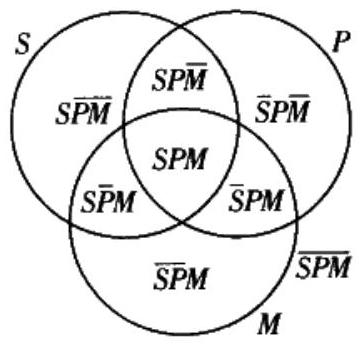
\includegraphics[max width=\textwidth, center]{2025_05_15_6a28331d5e7c993ad07ag-274}

图6-1\\
以瑞典人的类( $S$ )、农民的类( $P$ )和音乐家的类 $(M)$ 为例,可以作如下解释。SPM 是这三个类的积,由所有瑞典农民音乐家组成。SPM是前两个类与第三个类之补的积,由不是音乐家的瑞典农民组成。S $\bar{P} M$是第一、第三个类与第二个类之补的积:所有不是农民的瑞典音乐家组成的类。 $S \overline{P M}$ 是第一个类与其他两个类之补的积:所有不是农民也不是音乐家的瑞典人组成的类。接下来, $\bar{S} P M$ 是第二、第三个类与第一个类之

补的积:所有不是瑞典人的农民音乐家组成的类。 $\bar{S} P \bar{M}$ 是第二个类与其他两个类之补的积:所有不是瑞典人也不是音乐家的农民组成的类。 $\overline{S P M}$ 是第三个类与前两个类之补的积:所有不是瑞典人也不是农民的音乐家组成的类。最后,$\overline{S P M}$ 是三个类的补的积:所有不是瑞典人、不是农民,也不是音乐家的事物组成的类。

我们把注意力集中到标有 $P$ 和 $M$ 的两个圆上,显然,加上阴影或写人 $x$ 就能表示出 $P 、 M$ 构成的任何标准式直言命题,无论哪个是主项哪个是谓项。例如,要用图表示命题"所有 $M$ 是 $P$"$(M \bar{P}=0)$ ,我们就把所有不包含在 $P$ 中的 $M$ 的部分加上阴影。这个区域,包括了标有 $S \bar{P} M$ 和 $\overline{S P M}$ 的部分,这样就形成了图6-2。

我们再把注意力集中到 $S$ 和 $M$ ,加上阴影或写人 $x$ 就能表示由 $S$ 、 $M$ 构成的任何标准式直言命题,无论它们出现的顺序。要用图表示命题 "所有 $S$ 是 $M$"$(S \bar{M}=0)$ ,我们就把所有不包含在 $M$ 中的 $S$ 的部分加上阴影。这个区域,包括了标有 $S \overline{P M}$ 和 $S P \bar{M}$ 的部分。这样就形成了图 6-3。

现在,利用三个交叉的圆,就可以在一个图中同时表示两个命题——当然,条件是其中只出现三个不同的项。这样,"所有 $M$ 是 $P$"和"所有 $S$ 是 $M$"可以同时表示在图6-4中。\\
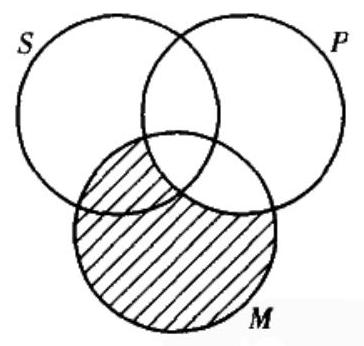
\includegraphics[max width=\textwidth, center]{2025_05_15_6a28331d5e7c993ad07ag-275(2)}

图6-2\\
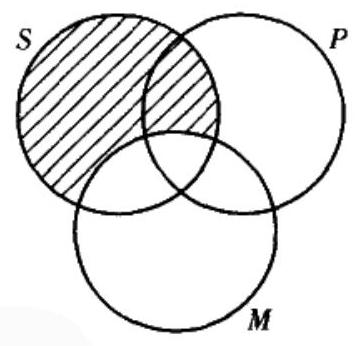
\includegraphics[max width=\textwidth, center]{2025_05_15_6a28331d5e7c993ad07ag-275(1)}

图6-3\\
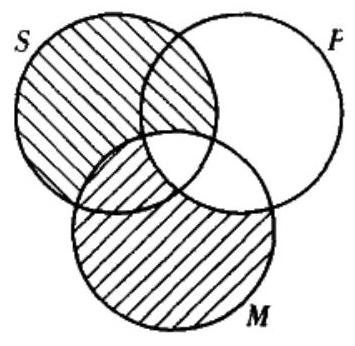
\includegraphics[max width=\textwidth, center]{2025_05_15_6a28331d5e7c993ad07ag-275}

图6—4

这正是三段论 AAA-1 的两个前提:

此三段论是有效的,当且仅当两个前提蕴涵或曰能推出结论,即两个前提已断言了结论所断言的东西。因此,在文恩图中画出有效论证的前提,也就已经把结论画出来了,而不需要画更多的圆。结论"所有 $S$ 是 $P$"的文恩图,应为在标有 $S \overline{P \bar{M}}$ 和 $S \bar{P} M$ 的部分加上阴影。我们看到表示两个前提的文恩图,也确实已经把结论表示了出来。这种情况说明 AAA- 1 一定是有效式。 ${ }^{[3]}$

我们再用文恩图检验一个明显无效的三段论:

所有狗是动物,\\
所有猫是动物,\\
所以,所有猫是狗。

用文恩图表示两个前提就是图6-5。\\
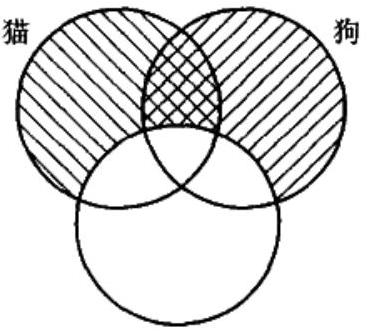
\includegraphics[max width=\textwidth, center]{2025_05_15_6a28331d5e7c993ad07ag-276}

动物

图6-5\\
在这个图中,$S$ 指称所有猫组成的类,$P$ 指称所有狗组成的类,而 $M$指称所有动物组成的类,$S \overline{P M} 、 S P \bar{M}$ 和 $\bar{S} P \bar{M}$ 部分已经加上了阴影,但结论却没有被表示出来,因为 $S \bar{P} M$ 部分没有阴影,要图示结论就必须把 $S \overline{P M}$ 和 $S \bar{P} M$ 两部分都加上阴影。这样,就能看出 AAA-2 的两个前提的图示并没能表示结论,这证明结论的断定超出了前提,前提并不蕴涵结论。而一个前提不蕴涵结论的论证是无效的,所以,我们所画出的图示证明了这个三段论是无效的。(实际上,它证明任何形如 AAA-2 的三段论都是无效的。)

如果我们用文恩图检验由一个全称前提和一个特称前提构成的三段论,那么,很重要的一点是:要首先在图中表明全称前提。举例来说,要

所有艺术家都是自我主义者,\\
有艺术家是乞亞,\\
所以,有乞丐是自我主义者。

我们应当先画出全称前提"所有艺术家都是自我主义者",再写人 $x$ 表示特称前提"有艺术家是乞丐"。正确的图示见图 6-6。\\
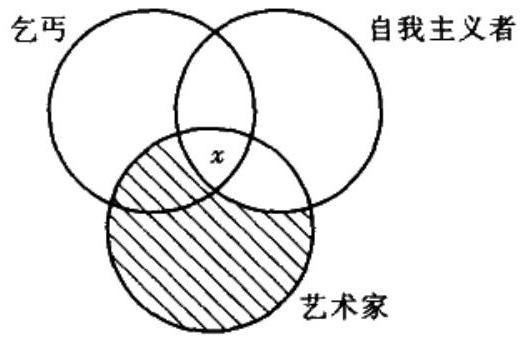
\includegraphics[max width=\textwidth, center]{2025_05_15_6a28331d5e7c993ad07ag-277}

图6-6\\
$S \bar{P} M$ 连同 $\overline{S P} M$ 两个部分表明的是全称前提,如果在给这两个部分加上阴影之前,试图先表明特称前提,我们就不能确定到底该把 $x$ 加在 $S P M$ 部分还是 $S \bar{P} M$ 部分,或者两个部分都加上。如果加在 $S \bar{P} M$ 当中,或者加在这部分与 $S P M$ 的交界处,那么加在 $S \bar{P} M$ 中的阴影就让图的原意变得含混不清。既然前提中包含的信息已经表示在图中了,检验时就看它是否也表明了结论。如果结论"有乞丐是自我主义者"能被表示出来,就应该把 $x$ 放在"乞甹"和"自我主义者"两个类的交叉部分。这个部分既包含了 SPM 也包含 SPM 部分,它们共同表明 SP。此三段论的结论所断定的东西,已经在表示前提的图示中表明了,因此,这个三段论是有效的。

再来看另一个例子,对这个例子的讨论将说明文恩图一个更重要的作用。考虑论证:

\begin{displayquote}
所有大科学家都是大学毕业生,有职业运动员是大学毕业生,
\end{displayquote}

首先在 $S P \bar{M}$ 和 $\bar{S} P \bar{M}$ 部分加上阴影,这样就表明了全称前提(见图6— 7),但我们仍然不明白应该把 $x$ 加到哪一部分才能表明特称前提。特称前提是"有职业运动员是大学毕业生",所以 $x$ 必须加在标有"职业运动员"和"大学毕业生"的两个圆交叉的部分。但是,交叉的区域又包括两个部分:$S P M$ 和 $S \bar{P} M$ 。 $x$ 应该放到其中哪个部分呢?前提并没有告诉我们答案,如果任意选一部分把 $x$ 加上去,就可能在图中加上了一些前提中本来没有的信息——也就破坏了文恩图检验的有效性。如果在两个部分都加一个 $x$ ,也会超出前提的断言。但是,把 $x$ 放在两部分的交界线上,我们就正好表明了第二个前提,而没有提供任何更多的东西。 $x$ 放在交界线上,指的是有东西属于它们两个类中的一个,但确实没有说明到底属于哪一类。两个前提的完整图示见图 6--8。\\
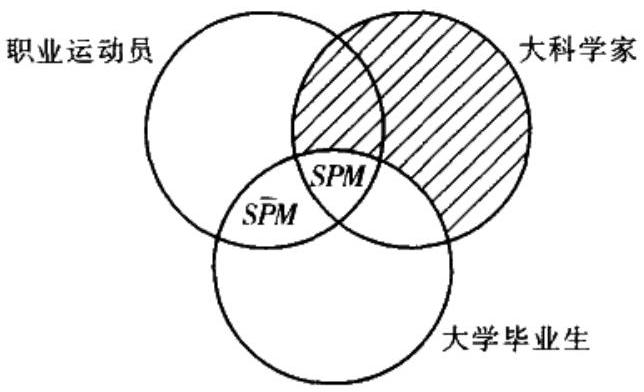
\includegraphics[max width=\textwidth, center]{2025_05_15_6a28331d5e7c993ad07ag-278}

图 6-7\\
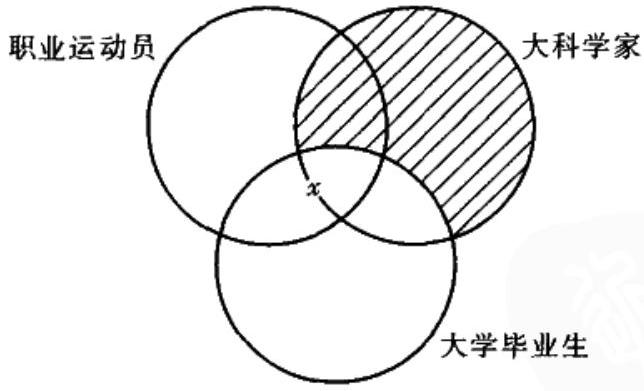
\includegraphics[max width=\textwidth, center]{2025_05_15_6a28331d5e7c993ad07ag-278(1)}

图6-8\\
通过考察,我们会发现前提的图示中并没有把结论表达出来。要表明结论"有职业运动员是大科学家",就必须要加一个 $x$ 在上面两个圆的交叉部分,或者加在 $S P \bar{M}$ 中,或者加在 $S P M$ 中。前面一个部分已经被加上阴影排除出去了,当然就不会包含 $x$ 。但图示也并没有显示 $S P M$ 中有 $x$ 。确实,\\
$S P M$ 或者 $S \bar{P} M$ 之中必有一个元素,但这个图示并没有说明究竟是在前者当中,还是在后者当中,因为前提就没有说明这一点。所以,结论就可能为假。当然,我们由此并不能确定结论就是假的,而只能知道结论没有被前提断定或蕴涵。但这已足以告诉我们论证是无效的。这个图也充分说明并非只有给定的这个三段论是无效的,而是所有形如 AII-2 的三段论都是无效的。

使用文恩图检验标准式三段论的一般做法可以总结如下:首先,在三圆的文恩图上标记三段论的三个项。接下来,把两个前提在图中都表示出来,如果一个前提是全称、另一个是特称的话,要首先标明全称前提。特别注意,如果特称前提并没有明确表明应该把 $x$ 加在哪一部分时,就把 $x$放在两个部分的交叉线上。最后,检查图示中是否已经包含了结论:如果包含了,那么三段论就是有效的,否则就是无效的。

使用文恩图区分三段论有效性与无效性的理论依据是什么?这个问题的答案可分为两个部分。首先,必须结合 6.2 节讲到的三段论论证的形式性质来讨论。那一节讲过,对给定三段论有效还是无效的一种合理检验是去判定另外一个三段论的有效性如何,而这个三段论与要考察的三段论恰有相同的形式。这种方法正是文恩图解法的基本依据。而说明文恩图解法如何达到这种检验目标,就构成问题解答的第二部分。

三段论一般都是就对象类而言的,其中的对象并不都呈现在我们面前,比如音乐家的类、大科学家的类、钠盐的类等等。这些类之间的包含或排斥关系可能是由论证得出的,也可能是在科学研究过程中经验地发现的。但它们绝不会自己呈现出来,因为涉及的类的元素不可能全部展现出来接受观察。但我们可创设一种情形,在这种经特殊界定的情形中,所涉及各个类的元素都可以呈现在人们面前以供直接观察,从而可以构造关于这种自设情形的三段论论证。文恩图本来是为表示标准直言命题而发明的,但其亦属于一种创设情形,一种可以使用各种工具在纸上、在黑板上绘制出来的情形。其所表示的命题亦可以解释为指涉图形本身。兹举一例即可说明。假如我们有这样一个关于分布在世界各地的各色人等的特殊三段论,其词项分别指称成功人士、热爱工作者和心猿意马者(工作中注意力分散者):

所有成功人士都是热爱工作者,没有热爱工作者是心猿意马者,

所以,没有心猿意马者是成功人士。

它的形式是 AEE-4,即:

所有 $P$ 是 $M$ ,\\
没有 $M$ 是 $S$ ,\\
$\therefore$ 没有 $S$ 是 $P$ 。 
\section*{6.4 三段论规则和三段论谬误}
在许多情况下,一个三段论并不能真正推得其结论。为帮助人们避免常见的错误,人们制定了一系列规则(本书列出六条)用来范导论证:对于任何给定的标准式三段论,通过考察其中是否有违反规则的情况,就能对它进行评判。

违反任何一条规则都会导致错误。这是一种特殊种类的论证错误,所以我们称之为三段论谬误;又因为这种错误是论证形式方面的,所以称之为形式谬误(与第4章所讲非形式谬误相对照)。在三段论论证中,必须谨防违反规则,避免产生谬误。每一种形式谬误都有一个传统名称,以下详加介绍。

\section*{规则1 避免四项}
一个有效的标准式直言三段论必须仅仅包含三个项,在整个论证中,每一个项都须在相同的意义上使用。

在直言三段论中,结论断定了两个项即主项(小项)与谓项(大项)之间的关系。因此,只有前提断定的是这两个项分别与同一个第三项(中项)的联系时,结论才能是合理的。如果前提不能做到这一点,就不能在结论的两个项之间建立联系,论证就不能进行。所以,每个有效的直言三段论必须只有三个项——不能多也不能少。如果包含了多于三个的项,三段论就是无效的。这种谬误叫做四项谬误。

这种谬误通常源于语词歧义,即用同一个词或短语表达两种不同的含义。最常见的是中项的含义发生转换,同一个词以某种用法与小项发生联系,而以另一种用法与大项发生联系。这样一来,与结论中的两个项发生联系的是两个不同的项(而不是同一个中项),所以结论断定的关系也就不能成立。 ${ }^{[4]}$

本章开始定义"直言三段论"时,就指出每一个三段论一定有且只有三个项。 ${ }^{[5]}$ 所以,可以把这个规则("避免四项")看做是一个论证成为一个真正的三段论的保证。

\section*{规则2 中项至少在一个前提中周延}
如果(如 5.3 节所说明)命题述及一个项所指称的全部对象,该项在命题中就是"周延"的。如果中项在两个前提中都不周延,推出结论所需要的词项关联就不能建立。

历史学家芭芭拉•塔克曼(Barbara Tuchman)认为,许多无政府主义的早期批判家是以下面这样一个"无意识的三段论"为依据进行论证的。

\begin{displayquote}
所有俄国人是革命者,所有无政府主义者是革命者,
\end{displayquote}

\begin{displayquote}
所以,所有无政府主义者是俄国人。 ${ }^{[6]}$
\end{displayquote}

这个三段论显然是无效的。错误在于它根据无政府主义者、俄国人两个类分别与革命者的类之间的联系,断定了前两个类的关系——但革命者这个项在两个前提中都是不周延的。第一个前提没有述及全部革命者,第二个前提同样没有。"革命者"在论证中做中项,如果它在三段论两个前提中都不周延,那么三段论就不可能是有效的。这样的谬误叫做中项不周延谬误。

这个规则的依据是小项和大项之间的联系需要中项做中介。而要建立这种联系,结论的主项或者谓项就必须与中项所指称类的全部对象相关联。否则,结论中的两个项就有可能分别与中项的不同部分发生联系,因而不必然与另一个项相关联。

这恰好是上面给出的三段论所存在的问题。俄国人只包含在革命者类的一部分当中(据第一个前提),无政府主义者也只是包含在革命者类的一部分之中(据第二个前提)——这两部分却是与另一个类(三段论的中项)的不同部分发生联系的,所以,中项就不能成功地联结小项和大项。一个有效的三段论,其中项必定至少在一个前提中周延。

规则 3 在结论中周延的项在前提中也必须周延\\
述及一个类的全部对象,比述及其中某些对象要断定更多。所以,如果三段论前提中不周延的项在结论中周延,也就是结论断定了比前提更多

东西。但是,有效的论证要求其前提必须能逻辑地推出结论,结论绝不能比前提断定得更多。可以说,在结论中周延而在前提中不周延的项确实是个信号,说明结论超出了前提,跑得太远了。这种谬误叫做不当周延。

结论可能是小项(主项)超出了前提,或者大项(谓项)超出了前提。所以,不当周延有两种不同形式,我们分别给它们一个名字:

大项不当周延("非法大项"),\\
小项不当周延("非法小项")。\\
举个例子来说明第一种,看下面这个三段论:

\begin{displayquote}
所有的狗是动物,没有猫是狗,
\end{displayquote}

\begin{displayquote}
所以,没有猫是动物。
\end{displayquote}

很明显,这个论证是不对的,但错在哪里呢?就错在结论是对所有动物的断言,即结论断定的是所有动物都在猫的类之外,而前提并没有对所有动物做出断言——故结论不当地超出了前提的断定。由于"动物"在三段论中做大项,所以此处的谬误就是非法大项。

再举个例子来说明第二种,看下面这个三段论:

所有传统教徒都是原教旨主义者(fundamentalist),所有传统教徒都是宽容筀胎行为的,

所以,所有宽容塈胎行为的都是原教旨主义者。

我们立刻会感觉到这个论证也有问题,其错误就在于:结论断定了所有堕胎行为的宽容者,而在前提中并没有这样的断言,没有述及所有宽容堕胎行为者的情况。这样,结论就不能为前提所担保。这个例子中"宽容堕胎行为的"是小项,所以此处的谬误就是非法小项。

\section*{规则4 避免出现两个否定前提}
任何否定命题( $\mathbf{E}$ 或 $\mathbf{O}$ )都否认类的包含关系,断定一个类的部分或者全部被排除在另一类的全体之外。但是,由两个断定这种排斥性的前提不能得出结论中的联系,因此,不可能是有效的论证。这种错误叫做排斥

前提谬误。\\
理解这个谬误需要进一步思考。考虑三段论的小项 $S$ 、大项 $P$ 和中项 $M$ ,对于这三个项之间的联系,两个否定前提能告诉我们什么呢?它们说明 $S$(结论的主项)完全或部分地排斥 $M$(中项)的一部分或者全部,并且 $P$(结论的谓项)完全或部分地排斥 $M$ 的一部分或者全部。但是,不管 $\boldsymbol{S}$ 和 $\boldsymbol{P}$ 的关系如何,这些关系中的任何一个都可能成立。这样的否定前提不能告诉我们 $S$ 和 $P$ 之间究竟是包含还是排斥,究竟是全部地包含或排斥,还是部分地包含或排斥。因此,如果三段论的两个前提都是否定的,论证肯定是无效的。

规则5 如果有一个前提是否定的,那么结论必须是否定的\\
如果结论是肯定的,也就是说,如果它断言两个类中的一个( $S$ 或 $P$ )完全或部分地包含在另一个之中,那么,前提必须断定这样的第三个类存在才能推出结论,即第三个类必须包含第一个并且被第二个包含,而类之间的这种包含关系只能由肯定命题表示。所以,肯定的结论只能由两个肯定的前提得到。违反这条规则的错误叫做从否定推肯定谬误。

要想得出肯定结论必须要有两个肯定前提,如上所述,我们可以确定地说,只要两个前提中有一个是否定的,结论就必须也是否定的,否则论证无效。

与其他谬误不同,这个谬误并不常见,因为对于任何从否定前提得肯定结论的论证,很容易就可以看出是极不合理的。举一个例子就能说明:

\begin{displayquote}
没有诗人是会计,有艺术家是诗人,
\end{displayquote}

所以,有艺术家是会计。

立即可以看到,由第一个前提对诗人和会计的排斥关系的断言,已使得该论证不可能为艺术家和会计之间的包含关系提供任何有效辩护。

规则 6 两个全称前提得不出特称结论\\
在直言三段论的布尔解释中(见5.6节),全称命题(A和E)没有存在含义,但特称命题( $\mathbf{I}$ 和 $\mathbf{O}$ )却有存在含义。只要像本书这样设定了布尔解释,就要避免从没有存在含义的前提得出有存在含义的结论。

最后这个规则在传统逻辑或者亚里士多德逻辑对直言三段论的解释中

并不需要,因为它们并不关心存在含义问题。但是,仔细考虑一下预设问题就会很清楚,如果一个论证的前提根本没有断定什么东西存在,但是从这些前提却推出了有些东西的存在,那么结论就是不合理的。这种错误叫做存在谬误。

下面这个例子就犯有这种谬误:

所有宠物都是家养动物,没有独角兽是家养动物,

所以,有独角兽不是宠物。

假如这个论证的结论是全称的"没有独角兽是宠物",它是完全有效的。在传统解释下,由于全称命题与特称命题一样都有存在含义,例子中的结论只是上述有效论证结论的"下位"。

但从布尔解释的角度说,上例的结论("有独角兽不是宠物")不仅仅是个"下位",因为特称命题与全称命题有很大不同。结论是特称的 $\mathbf{O}$ 命题,有存在含义,而 $\mathbf{E}$ 命题("所有独角兽不是宠物")是没有存在含义的。传统观点下接受的推论在布尔解释下不再被接受,因为在后者看来这样的论证犯了存在谬误一一种在传统解释下不会出现的错误。 ${ }^{[7]}$

以上给出的六条规则只适用于标准式直言三段论。它们提供了足够的工具,用以检验这一领域内任何论证的有效性。对于任一标准式直言三段论,如果违反了任一规则就是无效的,如果遵循了所有的规则就一定是有效的。 
\section{直言三段论的15个有效形式}

\begin{quotation}
在标准式直言三段论的256种可能形式中,只有15种是有效的。本节将介绍这些有效形式及其古典命名系统,帮助我们快速识别有效三段论并应用于实际推理中。掌握这些形式,是理解亚里士多德式推理系统的关键。
\end{quotation}

三段论的式取决于其中所含三个命题的类型(A、E、I、O)。直言三段论有64个不同的式,即这三个命题的64种可能组合:AAA、AAI、AAE等等,一直到$\cdots\cdots$EOO$、\mathrm{OOO}$。

三段论的格是其逻辑形状,由中项在前提中的不同位置决定。所以一共有四种不同的格,如果头脑中有一个图表或者用图标说明,就可以很清晰地记住这几个格,见图6—11:

\begin{center}
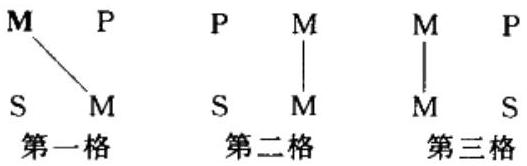
\includegraphics[width=\textwidth]{images/2025_05_15_6a28331d5e7c993ad07ag-288.jpg}

图6-11 三段论的四种格
\end{center}

\begin{center}
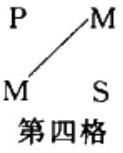
\includegraphics[width=\textwidth]{images/2025_05_15_6a28331d5e7c993ad07ag-288(1).jpg}
\end{center}

从图中可见:

\begin{itemize}
  \item 第一格的中项是大前提的主项、小前提的谓项;
  \item 第二格的中项在两个前提中都做谓项;
  \item 第三格的中项在两个前提中都做主项;
  \item 第四格的中项是大前提的谓项、小前提的主项。
\end{itemize}

64个式都可以有四个格。把两者结合起来,给定了三段论的式与格,也就唯一地确定了三段论的形式。因此,标准式直言三段论恰有$256(64 \times 4)$个可能的形式。

这些形式中绝大部分是无效的。根据前一节阐明的三段论规则,我们可以排除那些违反了一条或几条规则的形式,剩下的就是直言三段论的有效式。256个形式中,只有15个形式不能被排除,因而它们是有效的。\cite{patzig1968}

为更好地掌握三段论,古典逻辑学家给每一个有效式都起了独特的名称,每一个都完全刻画了其格与式。了解有效式的这个小集合,记住每一个有效形式的名称,对于我们实际运用三段论论证是很有帮助的。这些名称都是精心设计的,每个名称都包含了三个元音,代表着被命名三段论的式(依据标准的顺序:大前提、小前提、结论)。对于同式不同格的有效三段论形式,都分别给它们指派唯一的名称。例如,对于式为EAE的三段论,如果是第一格的就叫做Celarent,而如果是第二格的就叫做Cesare。\cite{lukasiewicz1957}

这些名称曾经有(现在仍然有)很实用的功能:如果懂得只有式与格的某些特定组合是有效的,并且通过名字就能识别那些有效论证,那么,无论给出任何式或格的三段论,就都能立即判定其正误。例如,AOO式只在第二格才是有效的。这个唯一的形式(AOO-2)就叫做Baroko。\cite{copi1980}熟悉Baroko并能很容易指认它的人就会确信这个式的其他格都是无效的,是必须拒斥的。

古典逻辑学家很细致地研究了这些形式,谙熟它们的结构和逻辑"感应"。这种精心设计好的逻辑系统,会使得一个人在言语或文本中碰到三段论论证时,能立即确切指认哪些是有效的,哪些是无效的。许多世纪以来,逻辑训练的一种常用方式,就是通过给出三段论有效形式的名称,来为三段论论证的可靠性进行辩护。而在激烈的日常论辩中具备这种迅速识别有效论证与无效论证的能力,一直被视为富有学养、思维敏锐的标志。而依赖演绎论证所建立起来的论证链条之坚固也得到了充分显示。一旦完全掌握三段论理论,这种实际论辩能力就会得到富有成效的令人愉悦的提升。

三段论论证曾经有如此广泛的应用,并被普遍视为学术论证最不可缺少的工具,因此,最先系统论述三段论理论的学术大师亚里士多德,得到了人们上千年的尊崇。他关于三段论的分析的论集迄今仍沿用着一个简单但令人肃然起敬的名字:Organon,即《工具论》。

作为这个著名逻辑体系的初学者,我们对三段论的掌握可能难以非常精通。但列出所有有效三段论形式并加以熟练掌握,无疑是最为有用的。15个有效三段论形式(布尔解释下的)可以根据格的不同分为四组:在前三个格中都有四个有效形式,第四格有三个有效形式。\cite{patzig1968}

下图即列出了15个有效形式,以及它们相应的传统名称:

\subsection{标准式直言三段论的15个有效形式}
\textbf{第一格}(中项在大前提中做主项、在小前提中做谓项):
\begin{itemize}
\item 1.AAA-1 Barbara
\item 2.EAE-1 Celarent
\item 3.AlI-1 Darii
\item 4.EIO-1 Ferio
\end{itemize}

\textbf{第二格}(中项在两个前提中都做谓项):
\begin{itemize}
\item 5.AEE-2 Camestres
\item 6.EAE-2 Cesare
\item 7.AOO-2 Baroko
\item 8.EIO-2 Festino
\end{itemize}

\textbf{第三格}(中项在两个前提中都做主项):
\begin{itemize}
\item 9.All-3 Datisi
\item 10.IAI-3 Disamis
\item 11.EIO-3 Ferison
\item 12.OAO-3 Bokardo
\end{itemize}

\textbf{第四格}(中项在大前提中做谓项、在小前提中做主项):
\begin{itemize}
\item 13.AEE-4 Camenes
\item 14.IAI-4 Dimaris
\item 15.EIO-4 Fresison
\end{itemize}

\footnotetext{(8)在传统或者亚里士多德式解释下,有效式的数目是19个或者24个,因为其中已包含了布尔解释下并不有效的弱化(weakened)格式——后者的结论比前提断定得更少。}
\footnotetext{(9)传统名称中所包含的元音是由拉丁语创造出来的一种记忆方法,其含义在拉丁语中是完备的;不过,无论说什么语言的人,都能通过观察名称中包含的元音,看出该三段论属于哪个式。}
\footnotetext{(10)传统的有记忆价值的名称是Baroco而不是Baroko;但在汉语中,似乎很难将c和k的发音分得很开,所以这里保持拼写一致用k取代c。}
\footnotetext{(11)第四格下有效三段论较少,是因为这种格式的三段论总是有点绕弯子,因而不太直接,似乎是人工制造的而不是自然思维的产物——但这也不影响其有效性。}

\begin{center}
\fbox{\parbox{0.95\textwidth}{
\textbf{本节要点}
\begin{itemize}
\item 标准式直言三段论共有\textbf{256种可能形式}(64个式 × 4个格)
\item 其中只有\textbf{15个有效形式}(布尔解释下)
\item \textbf{古典命名系统}:每个有效形式都有特定名称
  \begin{itemize}
  \item 名称中的三个元音对应三段论的式(大前提、小前提、结论)
  \item 例如:Barbara (AAA-1)、Celarent (EAE-1)、Baroko (AOO-2)
  \end{itemize}
\item \textbf{格的分布}:
  \begin{itemize}
  \item 第一格:4个有效形式
  \item 第二格:4个有效形式
  \item 第三格:4个有效形式
  \item 第四格:3个有效形式
  \end{itemize}
\item 掌握这些有效形式及其名称,有助于快速识别有效论证和无效论证
\end{itemize}
}}
\end{center} 
\section*{6.6 直言三段论 15 个有效形式的演绎推导}
直言三段论的 15 个有效形式是从 256 个可能形式中排除无效式以后得以确立的。我们可以通过确定哪些形式违反了三段论的基本规则来实行这种排除——演绎推导出三段论的 15 个有效形式。

对逻辑初学者来说,不必一定弄清如何排除无效式的细节。但对于那些从三段论分析的复杂性中获取乐趣的人而言,这应是一种虽有难度但令人愉悦的挑战。如果只想认识和把握三段论的有效式,即 6.5 节讲到的那些内容,就可以绕过本节不看。

这种演绎推导并不那么容易理解。从事这项工作必须清晰地记住以下两点:(1)6.4 节设定的六条三段论基本规则;(2)三段论四个格的模式,即图6-11。

根据结论的不同形式,我们首先把三段论的所有可能形式分为四组。每个结论都是 A、E、I、O 四种直言命题之一,没有其他可能,据此可以分四种情形考察一个有效的三段论需要具备什么特性,即可以这样提问:如果结论是 A 命题,通过某一条或几条规则能够排除什么形式;如果结论是 E 命题可以排除什么形式,以此类推。下面我们就逐个进行考察。

\section*{情形1:如果三段论的结论是 $\mathbf{A}$ 命题}
在这种情形下,前提不可能是 E 命题,也不可能是 O 命题,因为如果前提为否定命题的话,结论就应该是否定的(规则5)。所以,两个前提必定是 A 命题或 I 命题。小前提不能是 I 命题,因为小项(结论的主项,也就是一个 A 命题的主项)在结论中是周延的,如果小前提是 I 命题,那么在前提中不周延的项在结论中周延,违反了规则 3 。两个前提,即大前提和小前提,不能是 I 和 A,因为如果是的话,有两种可能,或者是在结论中周延的项在前提中不周延,违反规则 3 ,或者是中项两次不周延,违反规则2。所以两个前提(结论是 A 命题时)必须都是 A 命题,这意味着唯一有效的形式是 AAA 式。而第二格的 AAA 式会使中项两次不周延,第三格和第四格的 AAA 式都会造成前提中不周延的项在结论中周

延的错误。所以,如果三段论的结论是 A 命题,唯一的有效形式就是第一格的 AAA 式,即 AAA-1,传统上称这个有效形式为 Barbara。

情形 1 的总结:如果三段论的结论是 $\mathbf{A}$ 命题,只能有一种有效形式:\\
AAA-1-Barbara。

\section*{情形2:如果三段论的结论是 $\mathbf{E}$ 命题}
E 命题的主项和谓项都是周延的,因此,如果结论为 E 命题,三段论前提中的三个项也都必须至少周延一次 ${ }^{(1)}$ ,这只有当前提之一也是 E 命题时才有可能。但不能两个前提都是 E 命题,因为不能允许两个否定前提 (规则 4),同理可知另一个前提也不能是 O 命题。另一个前提也不能是 I命题,否则在结论中周延的项在前提中不周延,违反规则 3 。这样,另一个前提必须是 A 命题,两个前提的组合可能是 AE 或 EA。因此,在结论是 E 命题的情况下,可能的正确形式为 AEE 和 EAE。

如果是 AEE 式,它不能是第一格,也不能是第三格。因为如果是这两个格的话,结论中周延的项在前提中不周延。所以,有效的AEE式只能是第二格的,即AEE-2(传统上称为 Camestres),或者是第四格的,即 AEE-4(传统上称为 Camenes)。如果是 EAE 式,它不能是第三格,也不能是第四格,因为那也都导致结论中周延的项在前提中不周延。所以,有效的 EAE 式只能或者是第一格的,即 EAE-1(传统上称为 Celarent),或者是第二格的,即 EAE-2(传统上称为 Cesare)。

情形 2 的总结:如果三段论的结论是 $\mathbf{E}$ 命题,只能有四种有效形式: AEE-2、AEE-4、EAE-1 和 EAE-2——分别是 Camestres、Camenes、Celar- ent 和 Cesare。

\section*{情形3:如果三段论的结论是 I命题}
在这种情形下,前提不能是 E 或 O 命题,因为如果有一个否定前提的话,结论也应该是否定的。两个前提也不能都是 A 命题,因为结论为特称的三段论其前提不能都是全称的(规则 6)。同样,两个前提也不能都是 I 命题,因为中项必须至少在一个前提中周延(规则 2 )。这样,前提的组合必须是 AI 或者 IA,因而结论为 I 命题的三段论可能的有效形式为 AII 和 IAI。

AII 在第二格和第四格中不可能有效,因为中项至少要周延一次。因

\footnotetext{(1)据规则 $2 、 3$ 。
}此保留下来的 AII 式就是 AII-1(传统上称为 Darii)和 AII-3(传统上称为 Datisi)。如果是 IAI 式,它不能是 IAI-1 和 IAI-2,因为这两个形式都违反中项至少在一个前提中周延的规则。剩下的有效形式就是 IAI-3(传统上称为 Disamis)和 IAI-4(传统上称为 Dimaris)。

情形 3 的总结:如果三段论的结论是 I 命题,只能有四种有效形式: AII-1、AII-3、IAI-3 和 IAI-4——分别是 Darii、Datisi、Disamis 和 Dima- ris。

\section*{情形4:如果结论是 $\mathbf{O}$ 命题}
在这种情形下,大前提不能是 I 命题,因为结论中周延的项在前提中也必须周延。所以大前提可能是 A 命题、 E 命题或者 O 命题。

假设大前提是 A 命题。这样,小前提就不能是 A 命题和 E 命题,因为结论为特称( O 命题)时,前提不能都是全称的。小前提也不能是 I 命题,否则,或者中项一次也不周延(违反规则 2 ),或者结论中周延的项在前提中不周延。因此,如果大前提是 A 命题,小前提必须是 O 命题,结果就是 AOO 式。但在第四格, AOO 式不可能有效,因为中项两次不周延。在第一格和第三格也不可能有效,因为结论中周延的项在前提中不周延。因此当大前提是 A 命题时, AOO 式保留下来的有效形式只有第二格 AOO-2(传统上称为 Baroko)。

再假设(如果结论是 O 命题)大前提是 E 命题。在这种情况下,小前提将不能是 E 命题或 O 命题,因为不允许两个否定前提。小前提也不能是 A 命题,因为结论如果为特称的,前提就不能是两个全称命题(规则6)。因而只剩下了 EIO 式——它在四种格中都是有效的,传统上分别叫做 Ferio(EIO-1)、Festino(EIO-2)、Ferison(EIO-3)和 Fresison ( $\mathrm{EIO}-4$ )。

最后,假设大前提是 O 命题。同样小前提也不能是 E 命题或 O 命题,因为不能允许两个否定前提。小前提也不能是 I 命题,因为那样的话,或者中项一次都不周延,或者结论中周延的项在前提中不周延。因此,如果大前提是 O 命题,小前提必须是 A 命题,即必为 OAO 式。但要排除 $\mathrm{OAO}-1$ ,因为中项两次都不周延。也要排除 OAO-2 和 OAO-4,因为这两种情况都会使结论中周延的项在前提中不周延。于是就只剩下一个有效形式 OAO-3(传统上称为 Bokardo)。

情形4的总结:如果结论是 O 命题,则有六个有效形式:AOO-2、

\section*{EIO-1、EIO-2、EIO-3、EIO-4 和 OAO-3,分别叫做 Baroko、Ferio、Festi- no、Ferison、Fresison 和 Bokardo。}
以上的分析通过排除法证明了直言三段论恰有 15 个有效形式:结论是 A 命题时有 1 个,结论是 E 命题时有 4 个,结论是 I 命题时有 4 个,而结论为 O 命题时有 6 个。这 15 个有效形式中,四个是第一格的,四个是第二格的,四个是第三格的,三个是第四格的。这样,就完成了标准式直言三段论的 15 个有效形式的演绎推导。 
\section*{第6章概要}
第6章考察标准式直言三段论:组成成分、形式、有效性和制约其正确使用的规则。

6. 1 节给出了三段论大项、小项和中项的定义:

\begin{itemize}
  \item 大项:结论的谓项
  \item 小项:结论的主项
  \item 中项:两个前提中都出现,但结论中不出现的第三个项
\end{itemize}

继而又分别定义了大前提和小前提,包含大项的前提叫做大前提,包含小项的前提叫做小前提。如果几个命题出现的次序正好是:大前提在第一位、小前提在第二位、结论在最后,我们就把这样的三段论指定为标准式的。\\
6.1 节也说明了三段论的式与格是如何确定的。

三段论的式由识别三个命题类型的字母来确定,即A、E、I、O中的三个。总共有 64 个不同式。

三段论的格由中项在前提中的不同位置来确定。对四个可能的格描述并定义如下:

第一格:中项在大前提中做主项、在小前提中做谓项。\\
模式为:$M-P, S-M$ ,所以 $S-P$ 。\\
第二格:中项在两个前提中都做谓项。\\
模式为:$P-M, S-M$ ,所以 $S-P$ 。\\
第三格:中项在两个前提中都做主项。

模式为:$M-P, M-S$ ,所以 $S-P$ 。\\
第四格:中项在大前提中做谓项、在小前提中做主项。\\
模式为:$P-M, M-S$ ,所以 $S-P$ 。\\
6.2 节说明了标准式三段论的式与格如何共同地确定其逻辑形式。由于 64 个式每一个都有四个格,所以共有 256 个标准式的直言三段论,但其中只有一小部分是有效式。

6. 3 节介绍检验三段论有效性的文恩图方法,即在几个交叉的圆中,作上恰当的标记或涂上阴影以表示前提的含义。\\
6.4 节阐明标准式三段论的六条基本规则,同时定义了违反各条规则所造成的谬误。\\
-规则 1 一个有效的标准式直言三段论必须仅仅包含三个项,在整个论证中,每一个项都须在相同的意义上使用。

违反本规则所犯的错误:四项谬误。\\
-规则 2 在一个有效的标准式直言三段论中,中项必须至少在一个前提中周延。

违反本规则所犯的错误:中项不周延谬误。\\
-规则 3 在一个有效的标准式直言三段论中,在结论中周延的项在前提中也必须周延。

违反本规则所犯的错误:大项不当周延谬误,或者小项不当周延谬误。\\
-规则 4 任何有两个否定前提的标准式三段论都不是有效的。\\
违反本规则所犯的错误:排斥前提谬误。\\
-规则 5 如果一个标准式三段论有一个前提是否定的,那么结论必须是否定的。

违反本规则所犯的错误:从否定推肯定谬误。\\
-规则 6 一个有效的标准式直言三段论,如果结论为特称命题,那么其前提不能都是全称的。

违反本规则所犯的错误:存在谬误。\\
6. 5 节给出了标准式直言三段论的 15 个有效形式的说明,识别它们的格与式,并说明了它们传统的拉丁名称:

AAA-1(Barbara)、EAE-1(Celarent)、AII-1(Darii)、EIO-1(Fe- rio)、AEE-2(Camestres)、EAE-2(Cesare)、AOO-2(Baroko)、EIO-2\\
(Festino)、AII-3(Datisi)、IAI-3(Disamis)、EIO-3(Ferison)、OAO-3 (Bokardo)、AEE-4(Camenes)、IAI-4(Dimaris)、EIO-4(Fresison)。

6. 6 节展示了 15 个有效形式的演绎推导,通过排除法程序,证明了只有 15 个形式是完全遵守三段论的六条基本规则的。 

% 第七部分
\section{日常语言中的三段论论证}

\begin{quotation}
日常语言中的三段论论证往往不像标准式三段论那样整齐规范。本节将介绍如何识别和转换日常语言中的三段论论证,使其符合标准形式,便于进行有效性检验。
\end{quotation}

前几章考察的标准式直言三段论往往显得生硬、不自然。它们就像 "化学纯净物"一样,不含任何杂质和不相关的东西。但是,日常语言论证并不总是这么整齐划一地出现的。在此,我们更广义的使用\textbf{三段论}这一术语,用来指谓符合如下条件的任一论证:或者本来就是标准式直言三段论,或者是可以变形为标准式直言三段论而没有失掉或改变原意的论证。

三段论论证相当常见,所以我们要设法检验其有效性。但由于日常论证通常比标准形式松散,前面提到的检验方法——文恩图和直言三段论的规则一一不能直接适用于它们。日常的三段论论证形式变化多样,不可能为每一种形式都发明一个特殊的检验方法,除非有一种极度复杂的逻辑工具。要检验众多三段论论证的有效性,最明智的方法通常是:在不改变原意的前提下,把它们\textbf{变形}(reformulate)为标准式三段论。这个方法就是向标准形式的\textbf{化归}(reduction)或\textbf{翻译}(translation),最后得到的三段论叫做原给定三段论的\textbf{标准式翻版}。

评估日常语言三段论要满足两个条件。首先,要有一种便于应用的检验方法,将标准式三段论的有效式和无效式区分开来,这种方法我们已经有了(前面章节中讲到的图示和规则)。其次,要有一种翻译方法,将任何形式的三段论推理转变为标准形式,一旦掌握了这种方法,再用先前介绍的判定有效三段论的规则或文恩图解方法进行检验,我们就能评估任何三段论。

\subsection{非标准形式的三种偏离情形}

要说明将日常语言中的非标准三段论论证翻译为标准形式的方法,首先要区分非标准形式偏离标准形式的不同情形。下面是三种基本的偏离情形:

1.前提和结论的顺序不标准。这是小问题,因为如果仅仅是叙述的顺序不标准,很容易调整过来。

2.日常语言论证的构成命题中表面上包含不止三个项,但可以证明事实上并非如此。

3.日常语言论证的构成命题不都是标准式直言命题。

第二、三种偏离情形同样有可能翻译为标准形式,下面即讨论翻译方法。

\begin{center}
\fbox{\parbox{0.95\textwidth}{
\textbf{本节要点}
\begin{itemize}
\item \textbf{日常语言三段论}是可变形为标准式直言三段论而不失去或改变原意的论证
\item 检验日常三段论有效性的两个条件:
  \begin{itemize}
  \item 有将标准式三段论区分有效与无效的检验方法
  \item 有将任何形式的三段论推理转变为标准形式的翻译方法
  \end{itemize}
\item 日常语言三段论偏离标准形式的三种情形:
  \begin{itemize}
  \item 前提和结论顺序不标准
  \item 表面上包含超过三个词项
  \item 构成命题不都是标准式直言命题
  \end{itemize}
\end{itemize}
}}
\end{center} 
\section*{7.2 三段论词项数量的归约}
如果日常语言中的一个论证看起来有三段论的形式,但包含着三个以上的词项,那么不应该即刻把它看成犯了四项谬误,从而认为它是无效的。这样的论证往往能被翻译为与之逻辑上等价的只有三个词项且完全有效的标准形式三段论。完成这样的翻译要掌握两种方法:
(1)去除同义词。在应用文恩图或三段论规则之前,应当去除日常语言论证中的同义词。举例来说,这样一个论证:
没有富人(wealthy)是游民(vagrant),
所有律师(lawyer)都是有钱人(rich people),
所以,没有法律代理人(attorney)是流浪者(tramps)。
其中包含着"富人"、"律师"和"游民"的同义词。去除同义词之后,该论证可翻译为:
没有富人是游民,
所有律师都是富人,
所以,没有律师是游民。
这个三段论是标准的 EAE-1(Celarent),很明显是有效的。
(2)去除补类。有时仅仅去除同义词是不够的。来看下面这个论证,其中所有命题都是标准式直言命题:
所有哺乳动物是温血动物,没有蜥蜴是温血动物,
所以,所有蜥蜴都是非哺乳动物。
如果直接用第 6 章给出的三段论规则来检验,这个三段论违反了不止一个规则。一方面,它包含着四个词项:"哺乳动物"、"温血动物"、"蜥蜴"和"非哺乳动物"。另一方面,它从否定前提得到了一个肯定结论。但实际上这个推理是有效的。因为其中虽含有四个词项,但不是标准形式,不能直接用三段论规则检验。要想用第 6 章给出的几个规则来检验,必须首先把它翻译为标准形式。这是很容易的,因为四个词项中有两个 ("哺乳动物"和"非哺乳动物")互为补类。如果将结论进行换质,就可以减少词项的数量——翻译的结果是原论证的一个标准式翻版:

所有哺乳动物是温血动物,没有蜥蜴是温血动物,

所以,没有蜥蜴是哺乳动物。

它与原来论证的前提相同而结论等价,所以两者在逻辑上是等价的。这个标准式翻版遵守所有规则因而是有效的。其形式为 AEE-2(Camestres)。

尽管后者是最容易得到的,但它并不是唯一的标准式翻版。还可以对第一个前提进行换位、对第二个前提进行换质,而不改变结论,就可以得到另一个不同(但逻辑上等价的)标准式翻版。如下:

\section*{所有非温血动物是非哺乳动物,所有蜥蜴是非温血动物,}
所以,所有蜥蜴都是非哺乳动物。

这是一个 AAA-1(Barbara),也是遵守规则的有效式。对给定的三段论论证进行翻译,并没有唯一固定的标准形式,但如果其中一个是有效的,那么其他所有翻版都应该是有效的。

如果四个词项中有两个互为补类,那么任何含有这样的四个词项的三段论都可以化归为标准形式(或逻辑上等价的标准直言三段论);如果其中两个(或三个)与另外两个(或三个)互为补类,那么任何含有五个 (或六个)词项的三段论也都可以化归为标准形式。这种化归都是通过换位法、换质法、换质位法等直接推论而实现的,这些方法在 5.5 节都讲过。

一个三段论论证,其构成命题如果都是标准式直言命题,它有可能含有半打不同的词项,要把它化归为标准形式,进行一次直接推论是不够的。下面的例子就是一个六词项的三段论,但它的确是有效的:

没有非居民是公民,\\
所有非公民是非选举人,\\
所以,所有选举人都是居民。

可以用两种方法进行化归,第一种方法需要用到直接推论的三种方法,或许这是最自然也最明显的方法。首先把第一个前提换位再换质,把第二个前提换质位,于是得到如下一个标准式直言三段论:

所有公民都是居民,\\
所有选举人都是公民,\\
所以,所有选举人都是居民。

这也是一个 Barbara 式,用第 6 章阐明的任何一种方法都很容易证明它是有效的。 
\section{直言命题的标准化}

\begin{quotation}
本节介绍将日常语言中的非标准直言命题翻译为标准形式的九种方法。这些方法帮助我们将各种复杂的语言表达转换为可以用标准三段论规则和文恩图检验的形式,从而正确评估其有效性。
\end{quotation}

如 7.1 节所述,日常语言中三段论论证的形式可能偏离标准形式,不仅可能出现含有三个以上词项的情况(如 7.2 节讨论的那样),还可能有

这样的情况,即构成命题不都是标准的直言命题。显然,A、E、I、O命题有些生硬,而日常生活中许多三段论都是由非标准的命题组成的。要把这些论证化归为标准形式,就要把构成命题都翻译为标准形式。但日常语言内容丰富、形式多样,根本无法找出一套完善的翻译规则。在各种情形中,最关键的是理解已知的非标准命题的含义,这样才能在翻译时不丢失,也不改变原意。

尽管没有完善的规则,我们仍然可以介绍一些方便的方法,它们在处理某些特殊命题时常常十分有用。这些方法——本节介绍九种方法——只能被看做一种指针而不是规则,也就是说,它们是处理某些特定种类的非标准命题的技巧。

1.单称命题。有些命题肯定或否定的是一个特定的个体或对象属于某个类,例如"苏格拉底是哲学家"、"这张桌子不是古董"等。这样的命题叫做\textbf{单称命题}。它们肯定或否定的不是一个类与另一个类的包含关系 (像标准式直言命题那样),但我们可以把单称命题解释为处理类与类间关系的命题。可以按如下方式做到这一点:

每一个个体对象都对应着一个\textbf{单元类}(由一个元素组成的类),其中只有一个对象。这样,断定一个对象 $s$ 属于类 $P$ ,在逻辑上等价于断定了只含有一个元素的单元集 $S$ 完全包含于类 $P$ 之中。而断定一个对象 $s$ 不属于类 $P$ ,在逻辑上等价于断定只含有一个元素的单元类 $S$ 完全排斥在类 $P$之外。通常将这种解释看做自然而然的,无须调整记法。据此,我们就可以将任何一个单称肯定命题"$s$ 是 $P$"看做逻辑上等价的 A 命题"所有 $S$是 $P$"。同样,可以简单地将单称否定命题"$s$ 不是 $P$"看做逻辑上等价的 E 命题"没有 $S$ 是 $P$"——S 指称的都是只有一个对象 $s$ 的单元类。因此,不需要对单称命题进行明确的翻译,一般把它们分别归到 $\mathrm{A} 、 \mathrm{E}$ 命题当中。康德说过"在三段论中判断之使用,逻辑学者把单称判断类如全称判断处理,是很恰当的"${ }^{[1]}$ 。

然而,情况并不那么简单。特称命题有存在含义,而全称命题没有。在布尔解释下(如5.6节说明),如果机械地把单称命题当做三段论推理的 A、E 命题;再用文恩图或三段论规则来检验其有效性,就会出现严重的困难。

很明显,在某些情况中,可以把含单称命题的有效的两前提论证转化为有效的三段论。例如:

$$
\begin{array}{ll}
\text { 所有 } H \text { 是 } M, & \text { 可以变为三段论的 Barba- } \\
\frac{s \text { 是 } H,}{\therefore s \text { 是 } M_{0}} & \text { ra, 即 AAA-1 式, 很明显 } \\
\text { 是有效的 } &
\end{array}
$$

$$
\begin{aligned}
& \text { 所有 } H \text { 是 } M, \\
& \text { 所有 } S \text { 是 } H, \\
& \therefore \text { 所有 } S \text { 是 } M \text { 。 }
\end{aligned}
$$

但在另外的某些情形下,把含单称命题的有效的两前提论证转化为三段论,却是明显无效的。例如:

$$
\begin{array}{ll}
s \text { 是 } M, & \text { 得到的直言三段论是无效 } \\
\frac{s \text { 是 } H,}{\therefore \text { 有 } H \text { 是 } M_{0}} & \text { 的 AAI-3 式 }
\end{array}
$$

后者违反了规则 6 ,犯了存在谬误。\\
再者,如果把单称命题转化为特称命题,也会有同样的困难。有些情况下转化是有效的,例如:

\begin{center}
\begin{tabular}{lll}
所有 $H$ 是 $M$, & 可以变为三段论的 Darii, & 所有 $H$ 是 $M$, \\
$\frac{s \text { 是 } H,}{\therefore s \text { 是 } M \text { 。 }}$ & 即 AII-1 式,很明显是有效的 & 有 $S$ 是 $H$, \\
$\therefore$ 有 $S$ 是 $M$ 。 &  &  \\
\end{tabular}
\end{center}

但在另一些情况中,这种翻译却会得出明显无效的直言三段论。例如:

\begin{center}
\begin{tabular}{lll}
$s$ 是 $M$, & 得到的直言三段论是无效的 & 有 $S$ 是 $M$, \\
$\frac{s \text { 是 } H,}{\therefore}$ 有 $H$ 是 $M$ 。 & 有 $S$ 是 $H$, &  \\
$\therefore$ & 有 $H$ 是 $M$ 。 &  \\
\end{tabular}
\end{center}

后者违反了规则 2 ,犯了中项不周延谬误。\\
问题来自如下事实:单称命题要比任何一个标准式命题负载更多信息。如果把"$s$ 是 $P$"当做"所有 $S$ 是 $P$",那么,就丢掉了单称命题的存在含义,实际上这里 $S$ 非空。而如果把"$s$ 是 $P$"当做"有 $S$ 是 $P$",又漏掉了单称命题的全称性,即主项周延,它说的是全部 $S$ 是 $P$ 。

解决此问题的办法,就是把单称命题分析为两个直言命题的合取,即

一个单称肯定命题等价于相互关联着的 A、I 命题的合取。这样"$s$ 是 $P$"就等价于"所有 $S$ 是 $P$"合取"有 $S$ 是 $P$",单称否定命题则等价于"没有 $S$ 是 $P$"合取"有 $S$ 不是 $P$"。图7—1就是单称命题的肯定式和否定式的文恩图。在用三段论规则评估这种推理时,必须考虑它提供的所有信息,既考虑周延性也考虑存在含义。\\
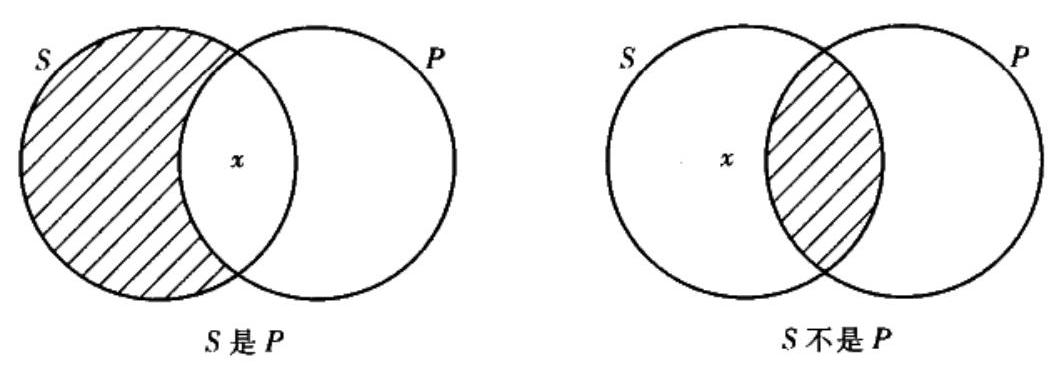
\includegraphics[width=\textwidth]{images/2025_05_15_6a28331d5e7c993ad07ag-310.jpg}

图7—1\\
对于含有单称命题的三段论,引用文恩图或规则检验其有效性时,只要我们记住其中有存在含义,就可以直接把它们看做全称(A 或 E )命题。

2.谓项为形容词或形容词短语,而非名词或类词项的直言命题。例如"有花是美的"、"没有战船是可调用的"都是直言命题,但"美的"和 "可调用的"表示的只是属性而不是类,所以它们的形式不标准,必须转化为标准形式。不过,每个属性都可以确定一个类,即具有这种属性的事物组成的类,所以对于每个这样的命题,都有一个相应的标准式直言命题。两个例句分别对应的是:I命题"有花是美的事物"和 E 命题"没有战船是可调用的事物"。如果一个直言命题的形式是标准的,只有谓项为形容词或形容词短语时,就把形容词或短语替换为这样一个词项,它指称由所有具有形容词表示之属性的事物所组成的类。

3.主要动词不是标准的联项"是"或"不是"的直言命题。常见的例子有"所有人都寻求赞誉"、"有人饮用希腊酒"。通常,转化的方法是把主项和量项之外的所有成分看做类的定义特征。先把能被替换的成分换成这样的词项,它们指称由类定义特征所确定的类,再改用标准的联项把它们同主项联结起来。这样上面两个例子就成了:"所有人是赞誉的寻求者"、"有人是希腊酒的饮用者"。

4.标准形式的各成分都出现,却没有按标准顺序排列的陈述句。"赛马全是良种马"和"结果好的事总是好事"就是这样的例子。在这种情形

下,首先要找出哪个是主项,然后再重新把各个成分排列一下,使之成为标准式直言命题。这种翻译通常都很直接。十分清楚,上述两个例句可翻译为"所有赛马是良种马"和"所有结果好的事是好事"。

5.量词不是"所有"、"没有"和"有"这些标准语词的直言命题。以 "每一"、"任何"等开头的陈述句很好转化。"每一只狗都有其得意之时"、 "任何贡献都会得到赞赏"可分别转化为"所有狗是有其得意之时的动物"和"所有贡献是会得到赞赏的事情"。"每一事物"、"任何东西"类似于 "每一"、"任一"。与此同一系列但限于人类的是"每人"、"任何人"、"无论谁"、"不管是谁"、"那些……的人"以及"每个......的人"等等。以上各表达式都不会带来什么麻烦。

语法冠词"a"和"an"("一个"等)也可用于指代量词,必须依据当时的语境,确定它们的意思是"所有"还是"有"。例如,"A bat is a mammal"(一只蝙蝠是一个哺乳动物)与"An elephant is a pachyderm" (一头大象是一个厚皮动物)可以合理地解释为"所有蝙蝠都是哺乳动物"与"所有大象都是厚皮动物"。但"A bat flew in the window"(一只蝙蝠飞进窗户)和"An elephant escaped"(一头大象逃跑了)显然指的是 "有蝙蝠是飞进窗户的动物"和"有大象是逃跑的动物"。

冠词"the"("这"、"这些"等)既可以用于指称一个特定的个体,也可以指称一个类的全部元素,有可能引起混淆。例如"The whale is a mammal"(鲸是哺乳动物)这句话,在一般情况下都会被理解为"所有鲸都是哺乳动物",而单称命题"The first president was a military hero" (第一任总统是军旅英雄)可以说是标准形式的 A 命题(一个有存在含义的单称命题),其道理本节前面已经讨论过了。 ${ }^{[2]}$

尽管以"每一"和"任一"开头的肯定句都可以译为"所有 $S$ 是 $P$",但对于以"not every"(并非每一个)和"not any"(并非任一)开头的否定句,却有很大区别。它们的译法不那么明确,需要更加小心。比如, "Not every $S$ is $P$"意思是有 $S$ 不是 $P$ ,而"Not any $S$ is $P$"意思是没有 $S$ 是 $P$ 。

6.排斥命题(exclusive propositions)。含有"只"(only)、"只有"(none but)的直言命题通常叫做\textbf{排斥命题},因为一般说来,它们断言的是谓项排他性地适用于主项。例如"只有公民能成为选民"、"只有勇敢者是值得公平对待的",第一句转化为标准形式是"所有能成为选民的是公

民",第二句转化为"所有值得公平对待的人是勇敢者"。以"只"、"只有"开头的命题一般可以按以下途径转化为 A 命题:将主、谓项互换位置,把"只有"换为"所有"。因此"只有 $S$ 是 $P$"和"只有 $S$'s 是 $P$'$s$"通常被理解为"所有 $P$ 是 $S$"。

但是,在某些语境中,"只"、"只有"被用于表达某种更多的含义。 "只有 $S$ 是 $P$"和"只有 $S$'s 是 $P$'$s$"表明的可能是"所有 $S$ 是 $P$"或者 "有 $S$ 是 $P$"。但这种情况并不常见。这个时候就需要语境的辅助了。如果没有附加信息,前面的翻译就是适当的。

7.不含量词的直言命题。例如"狗是肉食动物"、"孩子在场"。欠缺量词,句子的含义就不十分明确。只有考察它们所处的语境才能确定其含义,一般来说,考察之后就能把疑义清理掉。第一个例句"狗是肉食动物"很可能述及了所有的狗,可以转化为"所有狗都是肉食动物"。而第二个例句一般只述及某些孩子,转化为标准形式为"有孩子是在场的人"。

8.完全不像标准式直言命题但也可以有标准式翻版的命题。例如 "不是所有孩子都相信圣诞老人"、"有白色的大象"、"没有粉色的大象"以及"没有既圆又方的东西"。反思这些命题就会发现,它们在逻辑上等价于(因而可翻译为)下面的标准式命题:"有孩子不是相信圣诞老人的人"、"有大象是白色的事物"、"没有大象是粉色的事物"和"没有圆的东西是方的"。

9.除外命题(exceptive propositions)。还有一些这样的例子:"除了雇员(all except)都是合格的"、"雇员之外的人(all but)都是合格的"与"只有(alone)雇员不是合格的"。要把这样的\textbf{除外命题}翻译为标准形式,情况就会复杂一些,因为这种命题(与单称命题很类似)做出了两个而不是一个方面的断定。所给例子断言的不仅是所有非雇员是合格的,还断定了(在通常的语境中)没有雇员是合格的。如果把"雇员"记为 $S$ 、 "合格的人"记为 $P$ ,那么,这两个命题可以写成"所有非 $S$ 是 $P$"和 "没有 $S$ 是 $P$"。这两个命题是独立的,但联合起来就断定了 $S$ 和 $P$ 互为补类。

每个除外命题都是复合句,因此,不能转化为单一的标准式直言命题。确切地说,每一个除外命题应当翻译为一个合取式,即两个标准式直言命题的合取式。所以,上面关于合格性的三个例句都可以翻译为"所有非雇员是合格者,并且没有雇员是合格者"。

应该注意到,有些论证的有效性离不开数字或类数字(quasi-numeri- cal),但数字无法译为标准形式。这些推理本身就是非三段论的(asyllo- gistic)。因此,对它们进行分析就需要一种比直言三段论复杂一些的理论。当然,有些含有类数字量词的推理也可以用三段论分析。"几乎所有"、"并非全部"、"除少数几个之外都"、"几乎每个人"等就是这样的词。如果一个命题含有看起来像量词的词项,那么就可以处理为刚刚讲过的除外命题。下面几个除外命题都含有类数字:"几乎所有学生都参加了舞会"、"并非所有学生都参加了舞会"、"除少数几个之外,学生们都参加了舞会"和"只有一些学生参加了舞会",它们都肯定了有些学生参加了舞会,同时又否定了所有学生都参加了舞会。从三段论推论的观点看,它们给出的类数字信息并不相干,转化之后都是"有学生是参加了舞会的人,并且有学生不是参加了舞会的人"。

由于除外命题不是直言命题,而是合取式,含有这些命题的论证并不是我们所说的三段论论证。但是,对它们进行三段论分析和评估也未尝不可。含有除外命题的论证,要依据该命题所处的位置来进行检验。如果它是前提,那么就要分两次进行检验。举例来说,看下面这个论证:

\begin{quote}
每个看过比赛的人都参加了舞会,

不是全体学生都参加了舞会,

所以,有学生没有看过比赛。
\end{quote}

其中,第一个前提以及结论都是直言命题,很容易译为标准形式。但第二个前提是一个除外命题,不是简单句而是复合句。要检查前提是否蕴涵结论,首先要检验由论证的第一个前提、第二个前提的前一半以及结论组成的三段论。我们有:

\begin{quote}
所有看过比赛的人都是参加了舞会的人,

有学生是参加了舞会的人,

所以,有学生不是看过比赛的人。
\end{quote}

这个标准式的直言三段论是 AIO-2,违反了规则 2,犯了中项不周延的谬

误。但不能由此就得出结论说原来的论证是无效的,因为受检验的三段论只包含它的一部分前提。现在再来检验由第一个前提、第二个前提的后一半以及结论组成的三段论。译为标准形式后,得到一个非常不同的三段论:

所有看过比赛的人都是参加了舞会的人,\\
有学生不是参加了舞会的人,\\
所以,有学生不是看过比赛的人。

这是一个标准的 Baroko,即三段论的 AOO-2。很容易看出它是有效的。原来的三段论与这个有效式的结论相同,并且前者的前提包含着后者的前提,所以原来的论证也是有效的。因此,如果一个论证中有一个前提是除外命题,那么,对其有效性的检验要分为两次,即分别对两个不同的标准式直言三段论进行检验。

如果前提都是直言命题,但结论是除外命题,那么我们就可断言它是无效的。尽管两个直言命题可以蕴涵其中一个,即蕴涵结论复合句的一半,但不可能同时蕴涵两个。最后,如果两个前提和结论都是除外命题的话,那么,由原来论证所能建构的任何一个可能的三段论都要接受检验,才能确定其有效性。以上解释已足够处理这种情况了。

学会将多种非标准命题翻译为标准形式的技巧是很重要的,因为我们已经掌握的检验方法——文恩图解和三段论规则——只能直接用于标准式直言三段论。

\begin{center}
\fbox{\parbox{0.95\textwidth}{
\textbf{本节要点}
\begin{itemize}
\item 将非标准直言命题转换为标准形式的九种方法:
  \begin{itemize}
  \item \textbf{单称命题}:可将"苏格拉底是哲学家"视作"所有S是P",但须注意其包含存在含义
  \item \textbf{谓项为形容词的命题}:将形容词改写为对应的名词类型,如"美的"改为"美的事物"
  \item \textbf{非标准联项的命题}:将非"是/不是"动词改写为标准联项结构
  \item \textbf{顺序不标准的命题}:重新排列成分以符合标准顺序
  \item \textbf{量词不标准的命题}:将各类非标准量词("每一"、"任何"等)转换为标准量词
  \item \textbf{排斥命题}:"只有S是P"转换为"所有P是S"
  \item \textbf{不含量词的命题}:根据语境补充适当量词
  \item \textbf{非标准形式但可翻译的命题}:寻找逻辑等价的标准形式表达
  \item \textbf{除外命题}:翻译为两个标准式命题的合取
  \end{itemize}
\item 转换的核心原则是保持原命题的逻辑含义不变
\item 对含有除外命题的论证,需要分别对其组成部分进行有效性检验
\end{itemize}
}}
\end{center} 
\section*{7.4 协同翻译}
要对三段论论证进行有效性检验,其中总共只能包含三个项。有时做到这一点很难,需要比前面所述方法更细致的处理。请考虑命题"你总是与穷人为伍",显然,它既不是断言所有穷人总是在你身边,也不是说有些(特称的)穷人总是(always)在你身边。把该命题化归为标准形式的一种方法,也是一种最自然的方法,就是从其中的关键词"总是"着手分析。这个词意味着"在所有时间"(at all time),它表明原命题的一种标准式翻版为"所有时间都是你与穷人为伍的时间"。主、谓项中都出现的 "时间" 这个词可视为一个参项(parameter)。所谓参项,就是一个有助于以标准形式表达原来断言的辅助词项。

当然,绝不能机械地、不加思考地引入和使用参项,必须始终以所要翻译的那个命题为依据。命题"史密斯总是在台球比赛中获胜",显然断定的并不是史密斯从不间断地、始终在获胜!较合理的解释是,这句话是说:每当史密斯玩台球时,他就会获胜。如果这么理解,就可以直接把原句转化为"所有史密斯玩台球的时间是他获胜的时间"。并非所有参项都是时间性的。在对另一些命题进行翻译时,"地点"(place)、"情形"(case)也能被用做参项。例如"没有幻想的地方人类就会毁灭"(Where there is no vi- sion the people perish)和"每当琼斯迟到就丢失一次推销机会"(Jones lo- ses the sale whenever he is late)可分别译为:"所有没有幻想的地方都是人类毁灭的地方"和"所有琼斯迟到的情形都是他丢失推销机会的情形"。

在对三段论的三个构成命题进行协同翻译的过程中,参项的引人是必不可少的。一个直言三段论恰好包含三个项,要检验三段论就必须把它的构成命题都转化为标准式直言命题,其中只出现三个项。去除同义词以及换位法、换质法、换质位法的运用已经在 7.2 节讨论过。即使这样,还有很多三段论论证的项数仍然不能被缩减到三。此时,协同翻译就需要把同一个参项引到三个构成命题中去。请看下面这个论证:

\begin{displayquote}
哪里脏纸盒散落哪里就曾有不自爱者在此野餐,这里散落着脏纸盒,
\end{displayquote}

所以,一定有不自爱者在这里野餐过。

这个推理是完全有效的,但只有把前提和结论都翻译为标准式直言命题,并且其中只能有三个项,才能用文恩图或三段论规则来证明其有效性。第二个前提和结论能很自然地译为"有脏纸盒是散落在这里的东西"和"有不自爱者是在这里野餐过的人"。但这两个陈述句当中有四个不同的项。要把给定的论证化归为标准形式,就需要在三个命题中使用同一个参项。我们从第一个前提着手寻找这个参项,然后再用同样的参项去翻译第二个前提以及结论。"哪里"一词表明可以用"地方"作为参项。如果翻译三个命题时都用这个参项,则论证可变为:

所有散落脏纸盒的地方是不自爱者野餐过的地方,这个地方是散落脏纸盒的地方,所以,这个地方是不自爱者野餐过的地方。

这个标准式直言三段论的形式为 AAA-1,即 Barbara,是一个已经被证明有效的形式。

利用参项使表达式标准化的方法不是很容易掌握的,但有些三段论论证的确无法用其他方法进行翻译。再看一个例子有助于弄清其中的技巧:

每当狐狸经过那里,猎犬一定会发出叫声,所以,狐狸走的一定是别的路,因为猎犬都很安静。

首先,我们必须明白上述论证说的是什么。要把"猎犬很安静"这句话理解为"猎犬此时此地没有发出叫声"。这一步是去除同义词的必需步骤,因为第一个命题说的是"猎犬发出叫声"。同样,"狐狸走的一定是别的路"的结论,应理解为断言"狐狸没有经过那里"。第一个前提中的"那里"一词表明翻译时也可用"地方"做参项。于是,可得到这样一个标准式翻版:

$$
\begin{aligned}
& \text { 所有狐狸经过的地方是猎犬发出叫声的地方, } \\
& \text { 这个地方不是猎犬发出叫声的地方, } \\
& \text { 所以, 这个地方不是狐狸经过的地方。 }
\end{aligned}
$$

这个标准式直言三段论的形式为 AEE-2,即 Camestres,其有效性很容易确定。 
\section*{7.5 省略三段论(Enthymemes)}
三段论论证很常用,但其前提和结论并不总是都得到明确地陈述。常常只把论证的一部分表述出来,而其余部分就要靠"领会"了。比如,只提及"琼斯是个土生土长的美国人"这个前提,就可以得到结论:"琼斯是美国公民"。上述论证的表述并不完整,但很容易根据美国宪法把省略的前提补出来。加上被省略了的前提,完整的论证就是:

\begin{displayquote}
所有土生土长的美国人是公民,\\
琼斯是土生土长的美国人,\\
所以,琼斯是美国公民。
\end{displayquote}

完整表述后,这个论证就是一个直言三段论,其形式为 AAA-1,即 Bar- bara,它完全有效。如果一个推理是不完整的,其中有一部分需要"领会"或仅仅"在心中",我们就称之为省略三段论。省略(enthymematic)是不完整三段论的特征。

在日常话语甚至科学中,许多推论都是省略式的。原因不难理解,因为有相当一部分命题是公共知识。对于那些广为人知或无关紧要的真命题,听众和读者很容易就能想到并且补充完整,说话者和写作者就不再重复以减少麻烦。另外,用省略式描述推理,能够增加修辞效果,比描述出所有细节更强、更有说服力。亚里士多德在其著作《修辞学》中写道: "基于省略三段论的……演讲更受人欢迎。"

由于省略式不完整,所以要检验其有效性必须找到被省略的部分。如果省去的是一个必不可少的前提,缺了它推论就是无效的。但是如果省略的前提很容易补出来,评估时应该把它包括在论证当中才是公平的。这时,要假定论证者心中所想比明确说出的信息更多些。大多数情况下,很容易将说话人(或写作者)想到而没有表达出来的前提补充完整。举例来说,要说明"银色马"的怪事,神探福尔摩斯构造了这样一个推论,其中就省略了关键性前提,但是很容易猜到:

马厩中有一条狗。然而,尽管有人进来,并且把马牵走,狗却没有出声……显然,来者是这只狗非常熟悉的人物。

我们都能很好地理解其中暗含的意思:如果来者是陌生人,狗就会发出叫声。把这个前提看做福尔摩斯论证的一部分,对作者柯南-道尔来说才是公平的。

补充隐藏的前提时最重要的原则是:说话人确实认为听者可以接受这个命题为真。因此,要是把结论本身当做隐藏的前提就太愚委了。如果论证者希望听者把它当做前提而不加证明,那就无须再作为论证的结论来表述。

任何论证都能以省略式表达,但得到最广泛研究的还是三段论的省略式,本节也只限于研究三段论的省略问题。根据未表述部分的不同,传统上把省略三段论分为几种不同的省略体。三段论的第一种省略体指不出现大前提的情形。上面的例子就是这种省略体。第二种省略体保留大前提和结论,而不出现小前提。例如"所有学生都是反对新规则的,所以,所有大二学生都是反对新规则的",这里的小前提是个明显为真很容易补充出的命题:"所有大二学生是学生"。第三种省略体中两个前提都出现,但未表述结论。下面就是这个类型的例子:

我们的观念超不出我们的经验:我们没有关于神圣的属性与\\
作为的经验:我们用不着为我这个三段论下结论:你自己能得出推论来。 ${ }^{[3]}$

检验省略三段论的有效性共需两步:首先恢复省略的部分,然后再检验。公正地表示出省去的命题,需要语境敏感性以及对说话者意图的理解。请看这样一个论证:"没有真正的基督徒是精神空虚的,但有些常去教堂礼拜的人是精神空虚的",其中没给出结论,属第三种省略体,那么,原本要得出的结论是什么呢?如果说话者是要得出"有些常去教堂的人不是真正的基督徒",那么,推理就是有效的(EIO-2,Festino);但是如果说话者想说的是"有些真正的基督徒不是常去教堂的人",那么,这个省略式就是无效的(IEO-2),犯了大项不当周延谬误。

但一般说来,语境可以无歧义地确定未表述的命题。例如根据最高法院的意见,控制州内性暴力的联邦立法("针对妇女的暴力行为法案")是违反宪法的,大多数法官的关键性论证如下:

在任何意义上,性暴力犯罪都不是经济行为……迄今为止,在美国的历史上最高法院的判例中,只有经济行为才适用控制州内行为的条款。 ${ }^{[4]}$

可以领会但没有明确表述的结论是:根据最高法院的长期实行的规则,性暴力犯罪不归国会控制。

检验第三种省略体,先要把前提和(显而易见的)结论变形为标准形式。首先陈述大前提(含有结论之谓项的前提),然后确定其式与格,如上例:

大前提:根据最高法院的规则,国会控制的所有行为是经济行为。

小前提:没有州内的性暴力犯罪是经济行为。\\
结论(并未表述但结合语境却很清楚):没有州内的性暴力犯罪是最高法院规定为国会控制的。

这个三段论的式为AEE,中项在两个前提中都做谓项,因此是第二个格,其形式是 Camestres——有效的三段论。

第三种省略体,在某些情况下,即使不结合语境也能看出是无效的——例如,两个前提都是否定的,或者都是特称的,或者中项不周延。如果这样的话,不可能得出有效的结论。因此,这种省略式在任何语境中都是无效的。

也可能有这样的情况,在省略的是论证的一个前提的情况下,只有加上一个高度不合理的前提,才能把论证写成有效式。此时,指出这一点就构成对省略三段论的一种合理批判(legitimate criticism)。当然,更具毁灭性的批判是:有些三段论无论补上什么样的前提(即使是不合理的前提),也不能成为有效的三段论。

省略三段论与普通三段论的区别,从本质上说是修辞上的,而不是逻辑上的。不需添加什么新规则就能处理省略式,它们终究要接受与标准直言三段论同样的检验。 
\section*{7.6 连锁三段论(Sorites)}
有时会出现一个三段论论证,其前提多于两个。如果其结论是由前提依次推得的,那么它就是有效的,否则就是无效的。例如下面这个论证,它的前提有四个:

所有外交官都是机敏的人,\\
有外交官是欠思考的人,\\
所有欠思考的人都是轻率的,\\
没有轻率的人是谨慎的,\\
所以,有谨慎的人不是机敏的。

这个论证可以通过一系列环环相扣的直言三段论来进行检验。如果能把这个链条上的所有三段论都写出来,那么,任何一个违反了三段论六条规则的三段论都会使整个推理无效。

上述论证中的结论("有谨慎的人不是机敏的")可以由前提"没有轻率的人是谨慎的"和一个未出现的命题共同推出,这个未出现的命题就是"有轻率的人是机敏的"。这个未出现的命题,正是前面三个前提的结论。这样,我们就可以从一个论证推出另一个来。第一个论证是:

所有外交官都是机敏的人,\\
有外交官是欠思考的人,\\
所有欠思考的人都是轻率的,\\
所以,有轻率的人是机敏的。

而第二个论证的两个前提是:第一个论证的结论,以及原论证的第四个前提("没有轻率的人是谨慎的")。第二个论证是:

有轻率的人是机敏的,\\
没有轻率的人是谨慎的,\\
所以,有谨慎的人不是机敏的。

这样,就可以分别检验这两个三段论了。如果两个都有效,原论证就有效。由于第二个论证(结论是"有谨慎的人不是机敏的")的前提中,"轻率的"是中项,但两个前提中都没有出现"机敏的人"(大项)和"谨慎的人"(小项),所以,它并不符合标准形式。第二个论证的大前提(其中有大项)是"有轻率的人是机敏的",小前提是"没有轻率的人是谨慎的"。

这样,第二个论证的形式就是 IEO-3。这个形式违反了规则 3,因为大项在结论中周延而在前提中不周延,因此犯了大项不当周延谬误。这样,原论证的第二个环节无效,就使得整个论证无效。

这种包含几个前提和若干结论的三段论,如果每一个结论都成为下一个三段论的前提,就称为连锁三段论(sorites)。如果这些前提都是以标准形式排列,也就是说,每个词项(除了第一个前提的主项和最后一个前提的谓项)都分别作为前提的主项和谓项出现,这样的连锁三段论就可以看做是标准式的。如下例所示:

所有 $A$ 是 $B$ ,\\
所有 $B$ 是 $C$ ,\\
所有 $C$ 是 $D$ ,\\
没有 $D$ 是 $E$ ,\\
所以,没有 $A$ 是 $E$ 。

任何一个标准形式的连锁三段论都可以通过依次进行的三段论推论而得到检验。例如上面的连锁三段论,就可以通过如下三个三段论进行检验:

(1)所有 $B$ 是 $C$ ,\\
所有 $A$ 是 $B$ ,\\
所以,所有 $A$ 是 $C$ 。

(2)所有 $C$ 是 $D$ ,\\
所有 $A$ 是 $C$ ,(前一个三段论的结论)\\
所以,所有 $A$ 是 $D$ 。

(3)没有 $D$ 是 $E$ ,\\
所有 $A$ 是 $D$ ,(前一个三段论的结论)\\
所以,没有 $A$ 是 $E$ 。

这里所有的三段论都是第一格的。第一个和第二个是 Barbara 式,第三个是 Celarent 式,它们都是有效的。因此,原连锁三段论是有效的。

一个连锁三段论的前提可以写成任何顺序,为了检验其有效性,需要先把它们整理为标准顺序。一个标准式连锁三段论的有效性(或无效性)取决于构成它的所有三段论的有效性(或无效性)。 
\section{析取三段论和假言三段论}

\begin{quotation}
本节讨论两种重要的三段论形式:析取三段论和假言三段论。这些三段论不同于直言三段论,它们涉及选言和条件关系,在日常推理中有广泛应用。我们将学习这些三段论的有效形式以及常见的相关谬误类型。
\end{quotation}

一个三段论就是包含两个前提的演绎论证。可以有许多不同种类的三段论,最常见、最重要的就是直言三段论,前面几章已经对它进行了详细的考察。本节将简要讨论其他几种三段论。

\subsection{析取三段论(Disjunctive Syllogisms)}
在一个析取(或"选言")三段论中,有一个前提是析取命题。例如:

或者傻瓜,或者无赖,\\
他不是傻瓜,\\
所以,他是个无赖。

这样的论证是有效的。 ${ }^{[1]}$ 传统上把这种论证形式称为"通过否定进行肯定"(modus tollendo ponens),即通过否定其中一个选言支来肯定另一个选言支。有效的析取三段论定义如下:

一个析取三段论是有效的,当且仅当其中一个前提是析取命题,另一个前提是对其中一个选言支的否定,而结论是未被否定的那个选言支。

这里讨论的析取命题指的是"弱的"或"可兼的"析取(见8.1节),意思是它断言的是至少有一个选言支为真,但可能两个都真。如果析取三段论的前提是一个强的(或"不可兼的")析取命题,即断言恰好只有一个选言支为真,另一个为假,那么,下面的论证形式也是有效的:

或者傻瓜,或者无赖,\\
他是个傻瓜,\\
所以,他不是无赖。

传统上把这种论证形式称为"通过肯定进行否定"(modus ponendo tollens),即通过肯定其中一个选言支来否定另一个选言支。

\footnotetext{(1)在第 8 章,我们会看到,这种形式以及其他形式的论证,都很容易用真值表加以验证。
}
大多数情况下,不通过语境就无法确定析取命题到底是强的还是弱的。但是,对于有效的析取三段论的定义,并不需要这种区分。这个定义对于两种析取命题都适用。

如果一个论证具有析取三段论的形式,但并不符合这里的定义,那么,这种论证就是无效的,它所犯的错误传统上称之为\textbf{肯定选言支谬误}。这种谬误往往出现在弱析取命题的论证中,比如"或者傻瓜,或者无赖。他是个傻瓜,所以他不是无赖"。如果"或者傻瓜,或者无赖"被解释为弱析取,那么,即使两个前提都真,结论也可能为假。因此,这样的论证是无效的。

\subsection{假言三段论(Hypothetical Syllogisms)}
标准形式的假言三段论包含两个假言命题作为前提,外加一个假言命题作为结论。例如:

如果第一个土著人是政客,那么他会说谎,\\
如果他说谎,那么他会否认自己是政客,\\
所以,如果第一个土著人是政客,那么他会否认自己是政客。

这个论证叫做\textbf{纯粹假言三段论},因为它的前提和结论都是假言命题。这种论证是有效的。 ${ }^{[1]}$

还有一种常见形式的假言三段论,它有一个假言前提,一个直言前提,以及一个直言结论。有两种这样的有效形式,在此要分别进行讨论。

第一种有效的形式,传统上称为\textbf{肯定前件}(modus ponens),例如:

如果第二个土著人说真话,那么只有他是政客,\\
第二个土著人说真话,\\
所以,只有他是政客。

这里,第一个前提是假言命题,第二个前提肯定了第一个前提的前件,而结论则肯定了第一个前提的后件。这种形式的任何论证都是有效的。

但是,如果一个论证具有与肯定前件相似的形式,但却不是有效的,这种错误就称为\textbf{肯定后件谬误}。例如:

\footnotetext{(1)同样,在第 8 章会看到,用真值表可以很容易证明这种形式的有效性。
}
如果培根写了《哈姆雷特》,那么培根是个大作家,\\
培根是个大作家,\\
所以,培根写了《哈姆雷特》。

显然,这个论证是无效的。第二个前提肯定了第一个前提的后件,而结论肯定了第一个前提的前件。

第二种有效的假言三段论,传统上称为\textbf{否定后件}(modus tollens),例如:

如果这位客人是陌生人,那么狗会叫,\\
狗没有叫,\\
所以,这位客人不是陌生人。

这里,第一个前提是假言命题,第二个前提否定了第一个前提的后件,而结论否定了第一个前提的前件。这种形式的任何论证都是有效的。

但是,如果一个论证具有与否定后件相似的形式,但却不是有效的,这种错误就称为\textbf{否定前件谬误}。例如:

如果洛克菲勒拥有福特汽车公司的全部黄金,那么洛克菲勒很富有,\\
洛克菲勒并不拥有福特汽车公司的全部黄金,\\
所以,洛克菲勒并不富有。

显然,这个论证是无效的。第二个前提否定了第一个前提的前件,而结论否定了第一个前提的后件。

\begin{center}
\fbox{\parbox{0.95\textwidth}{
\textbf{本节要点}
\begin{itemize}
\item \textbf{析取三段论}的特点:
  \begin{itemize}
  \item 一个前提是析取命题
  \item 有效形式:"通过否定进行肯定"(modus tollendo ponens)
  \item 对于强析取命题,"通过肯定进行否定"(modus ponendo tollens)也有效
  \item 常见错误:肯定选言支谬误
  \end{itemize}
\item \textbf{假言三段论}的类型:
  \begin{itemize}
  \item 纯粹假言三段论:两个假言前提,一个假言结论
  \item 混合假言三段论:一个假言前提,一个直言前提,一个直言结论
  \end{itemize}
\item 混合假言三段论的有效形式:
  \begin{itemize}
  \item \textbf{肯定前件}(modus ponens):如果P那么Q,P,所以Q
  \item \textbf{否定后件}(modus tollens):如果P那么Q,非Q,所以非P
  \end{itemize}
\item 混合假言三段论的常见谬误:
  \begin{itemize}
  \item \textbf{肯定后件谬误}:如果P那么Q,Q,所以P
  \item \textbf{否定前件谬误}:如果P那么Q,非P,所以非Q
  \end{itemize}
\end{itemize}
}}
\end{center} 
\section*{7.8 二难推论(The Dilemma)}
没有什么特别重要的地方。但从修辞角度看,二难推论是一种最有力量的说服工具之一一可谓论战中的一种致命性武器。\\
不严格地说,如果一个人必须在两种选项中做出决断,但两个选项都很糟糕或令人不愉快,那么,我们就说这个人"陷人"了两难(或者说进退维谷)之中。二难推论就是一种旨在使对手陷人这样境地的论证方式。在争论过程中,二难推论使得对手必须做出选择,但无论选择什么,都会得出一个他不能接受的结论。

理查德•费曼(Richard Feynman)是一位著名的物理学家,他在回忆1986年"挑战者"号爆炸的调查时,猛烈地抨击了(美国)国家航空航天局(NASA)的管理失误,他用的就是下面的二难推论:

\begin{displayquote}
我们每次问起高层管理者,他们都会说关于手下发生的事,他们什么都不知道……或者最高领导团确实不知道,这样他们就不知道应该知道的事,或者他们知道,这样他们就在对我们说说。 ${ }^{[7]}$
\end{displayquote}

如此的质问就将对手(此处指的是国家航空航天局的管理者们)推人两难境地,令他们无地自容。其中唯一明确表述的前提是一个析取命题,但析取支必定有一个为真,或者他们知道或者他们不知道手下发生的事。不管选择哪一方,结果对对手来说都是不利的。二难推论的结论本身也可以是一个析取命题(例如,"国家航空航天局的管理者或者不知道他们应该知道的事,或者他们说谎"),此时我们称之为复杂式(complex)二难推论。结论也可以是直言命题,这时就称之为简单式二难推论。

二难推论的结论并非总是令人不愉快的,如下简单式二难推论得出的就是个好结论:

如果天上的神明没有欲求,那么他们就会很满足,如果他们有欲求而能完全实现,那么他们也会很满足。他们或者没有欲求或者能完全实现欲求。总之,他们都会很满足。

二难推论的前提并没有特殊的顺序要求,提供选项的析取前提可前可后。表述选择后果的两个条件命题可以联合表述,也可分开陈述。二难推论常用省略式表述,结论一般都是显而易见的,无须表述出来。有一个例子取

自林肯总统的一封信,他为废止美国南部邦黑奴制度的宣言作了如下辩护:

此宣言如同法律一样,或者有效或者无效。如果无效,就没必要取消。如果有效,就不能取消。任何人都明白。 ${ }^{[8]}$

避开或驳斥二难推论的结论的方法有三种,它们也有各自的名称,都与二难的两个(或多个)"死角"有关。分别称为"绕过(或避开)死角法"、"直击(擒拿)一角法"、"构造反二难法"。它们并非证明二难推论形式无效,而是在不改变推论形式有效性的前提下,寻找避免结论的方法。

绕过死角法是拒斥其析取前提。这是常用的最容易的避开二难的手段。除非析取前提的两个支命题是矛盾关系,否则它们很有可能是假的。常用来说明这个方法的例示是给学生分级打分的例子,有人认为好的分数能激励学生更努力地学习。但学生们想出这样一个二难推论用来驳斥上述理论:

如果学生喜爱学习,那么就不需要激励。如果学生厌烦学习,那么激励也没有用。学生或者是喜爱学习的或者是厌烦学习,所以,激励是不需要的或者没用的。

该论证形式是有效的,但我们能用绕过死角法来反驳这个论证。其析取前提是假的,因为学生会有不同的学习态度:有的喜爱,有的厌烦,还有许多人不同于前两者。对于后面这些人来说,激励既是需要的也是可以发挥作用的。这种方法并不是证明结论为假,只是表明推论本身并没有给结论提供充足的理由。

如果析取前提穷尽了所有可能性,是不可驳倒的,就不能用上述方法了。必须有另外的方法来避开结论,其中之一就是直击一角法,即拒斥两个假言前提中的一个。要否定两假言前提的组合,我们只需否定其中的一个即可。直击一角,就是要试图表明条件前提至少一假。刚才驳斥学校分级打分的例子,所依据的条件前提之一是"如果学生喜爱学习,就不需要激励",反驳者可以争辩说,即使一个学生喜爱学习,也需要激励,好分数会带来额外的奖励,甚至能激励最勤奋的学生更认真地学习。这样一

来,就很可能得到好的回应一一原来的二难的一角就被击破了。\\
构造反二难法是最巧妙的方法,但并不总能令人信服,我们来看这是为什么。用这种方法驳斥给定的二难推论,需要构造另一个二难推论,它的结论与原来的结论相反。辩驳中可以使用任何一个二难推论,但最理想的反二难推论应当与原来的推论有相同的组成成分(直言命题)。

有个古老的例子能说明这种方法,相传雅典有一位母亲劝儿子不要从政时说道:

如果你主持公道,人们就会仇视你。如果你不主持公道,神灵们就会仇视你。你必定或者主持公道或者不主持公道,所以无论如何都会被仇视。

他的儿子反驳说:

如果我主持公道,神灵们就会施爱于我。如果我不主持公道,人们就会施爱于我。我必定或者主持公道或者不主持公道,所以我都会被爱。

在把二难推论作为强力工具的日常论辩中一般人的争论中,这种驳斥方法,从几乎相同的前提得到相反的结论,是种很不错的修辞手法。但如果更细致地研究,就会发现它们的结论并不像初看上去那样对立。

第一个二难推论的结论是儿子会被仇视(被人们或者被神灵们),而反二难的结论是儿子会被爱(被神灵们或被人们)。实际上两者完全是相容的。反驳用的反二难仅仅是建构了一个结论不同的论证而已。两个结论可能都是真的,因而这里并没有达成真正的反驳。但在唇枪舌剑的辩论中,并不需要细致分析,如果在公共争辩中出现这样的反驳,听众大多会把它当做对原论证的毁灭性攻击。

如此反驳并不能驳倒推理,而只是将注意力引向同一事情的不同方面,这从如下的二难推论可能看得更清楚。"乐观主义者"认为:

如果我工作,就能挣钱,如果赋闲在家,那么我乐得自在。我或者工作或者不工作,总之,我能挣钱或者乐得自在。

\section*{而悲观主义者却会给出这样一个反二难:}
如果我工作,就不能乐得自在,如果赋闲在家,就不能挣钱。或者工作或者不工作,总之,我或者不能乐得自在或者不能挣钱。

这些结论只能说明看问题的视角不同,并非对事实状况的意见不一致。通常讲二难推论,都要说到普罗塔哥拉(Protagoras)和欧提勒士 (Euathlus)之间著名的讼案。普罗塔哥拉是生活在公元前 5 世纪的希腊的一名教师,他开设了很多课程,其中最著名的是法庭辩护术,欧提勒士想跟他学习当一名律师,但他负担不起学费。于是两人定了一个契约,普罗塔哥拉先不收学费,等欧提勒士学成并在第一场官司中获胜时,再交学费。可是,欧提勒士学成之后,迟迟没有在法庭上进行辩护,普罗塔哥拉等得不耐烦了,于是把他的学生告上法庭,要求收回学费。欧提勒士忘记了"律师为自己的案子辩护乃属愚行"的格言,决定为自己进行辩护。审理开始后,普罗塔哥拉就用一个压倒性二难推论陈述己方要求:

如果欧提勒士打输了官司,那么他必须还我学费(根据法庭的判决),如果欧提勒士打赢了官司,那么他也必须还我学费 (根据我们之间的契约),或者他打输或者打赢官司,都必须还我学费。

情况看来对欧提勒士而言十分不利,但他已把修辞术学得很好,于是他向法庭提出了如下相反的二难推论:

如果我打赢了官司,我不必交学费(根据法庭的判决),如果我打输了官司,我也不必交学费(根据我们之间的契约),或者我打赢或者打输,都不必交学费。

如果你是法官,该如何判决呢?\\
注意欧提勒士的反二难的结论与普罗塔哥拉的结论的确不相容,一个确实是另一个的否定。这种相反二难推论与原来的二难推论的互相拒斥的情况并不多见。在这样的情况下,前提就是不相容的,两个二难推论可用于澄清其中蕴涵的矛盾。 
\chaptersummary{
本章考察日常语言中的三段论论证。我们看到\logicterm{标准式三段论}的理论如何应用于这些论证。

日常语言中的三段论论证是逻辑学重要的研究对象,因为它们广泛存在于我们的日常交流、论辩和科学研究中。然而,这些论证往往不像教科书中的\logicterm{标准式三段论}那样整齐规范。本章介绍了一系列方法,帮助我们识别、\logicterm{翻译}和评估这些非标准的三段论论证。

7.1 节指出,日常语言论证很少以标准形式出现。要把它们\logicterm{翻译}为标准形式,需要理解它们的含义,而不能仅仅依赖表面的语法形式。这种\logicterm{翻译}过程需要对原始论证的真实意图有准确理解。

7.2 节解释如何把一个表面上有三至六个词项的论证归约为只有三个词项的\logicterm{标准式三段论}。这需要(1)去除同义词,以及(2)对某些词项\logicterm{换质}以处理其\logicterm{补类}。这种词项归约对于识别和评估看似复杂的论证非常关键。
}

7.3 节提出九种有用的方法,用以处理那些构成命题不是\logicterm{标准式}的三段论论证。这些方法包括:

1.\logicterm{单称命题},如"苏格拉底是哲学家",可当做全称命题(A 或 E)对待,但需注意其存在含义。

2.如果命题的谓项是形容词或形容词短语,可把它们替换为指称相应类的词项,使命题符合标准形式。

3.如果命题的主要动词不是标准联项"是"或"不是",可把动词及其他词语(主项与量项之外)看做类的定义特征,从而把原命题改写为\logicterm{标准式}。

4.如果命题的各成分虽已出现但顺序不标准,找出主项,重新调整各成分的顺序,使之符合标准形式。

5.处理非标准量词时,通常要把它们替换为"所有"、"没有"或"有"。要把"并非每个……"\logicterm{翻译}为"有……不是……"。

6.\logicterm{排斥命题},如"只有公民是选民",一般要通过颠倒主、谓项位置\logicterm{翻译}为 A 命题。结论通常是"所有选民是公民"。

7.不含量词的命题,要依据语境把量词"所有"或"有"补充完整,明确其逻辑含义。

8.有些命题的表达形式完全不像\logicterm{标准式直言命题},但其逻辑上等价的直言命题可以明确地表述出来。

9.\logicterm{除外命题},如"除了雇员之外所有人都合格",不是简单的直言命题,而要\logicterm{翻译}为两个\logicterm{标准式直言命题}的合取。

7.4 节说明并举例解释了\logicterm{协同翻译}的方法,即有时需要把同一个辅助词项(参项)引入三段论的三个构成命题中,以便把整个论证\logicterm{翻译}为标准形式。这种方法对于处理包含时间、地点、情境等关系的日常语言论证特别有用。

7.5 节考察\logicterm{省略三段论},即前提或结论未明确表述出来的三段论。我们看到,在对\logicterm{省略三段论}进行检验之前,如何发现并明确表述出未出现的命题。这种省略形式在日常论证中极为常见,理解它们需要敏感于语境和说话者意图。

7.6 节解释并举例说明\logicterm{连锁三段论}。\logicterm{连锁三段论}包含多个前提,形成一系列环环相扣的推理链条。检验这类论证的\logicemph{有效性},需要将其拆解为一系列\logicterm{标准三段论},并分别验证每个环节。

7.7 节解释了\logicterm{析取三段论}和\logicterm{假言三段论},指出了它们的\logicemph{有效}形式和可能产生的\logicwarn{谬误}。这两种三段论形式在日常推理中广泛应用,了解它们的\logicemph{有效}形式和常见\logicwarn{谬误}对于批判性思维至关重要。

7.8 节讨论\logicterm{二难推论}的各种形式,并说明了反驳\logicterm{二难推论}的三种方法:\logicterm{绕过死角法}(拒斥析取前提)、\logicterm{直击一角法}(否定条件前提)以及\logicterm{构造反二难法}(建立相反结论的二难推论)。\logicterm{二难推论}是强有力的修辞工具,了解其结构和应对方法有助于我们在论辩中保持清晰思考。

总之,本章提供了一套全面的工具和方法,帮助我们将复杂多样的日常语言论证\logicterm{翻译}为可以用标准规则检验的形式。这些技能不仅对于学术研究有价值,也对提高我们在日常生活中分析和评估论证的能力大有裨益。

% 参考文献将在主文档末尾统一显示

% 第八章
%\\section{现代逻辑的符号语言}

\begin{quotation}
本节介绍现代符号逻辑的基本概念和优势。与古典逻辑不同,现代逻辑使用专门的符号语言来避免自然语言的缺陷,能够更精确地表述论证,并简化复杂的推理过程。我们将学习为什么符号逻辑是分析演绎论证的强大工具。
\end{quotation}

我们一直在寻求对演绎论证进行分析和评估的技术。演绎理论旨在提供这样的技术,它已经发展出两个不同的分支来做这件工作:此前三章所考察的是经典逻辑或亚里士多德型逻辑,本章和下两章的主题则是现代符号逻辑。

然而,论证的分析和评估经常因其表述语言的特性(如英语或任何其他自然语言的特性)而非常困难。自然语言使用的语词可能是模糊的或歧义的,论证的结构可能是含混的,比喻和习语可能会引起混淆或误导,诉诸情感可能会引起混乱等,这些问题在第一部分已经探讨过了。要避免这些困难就要直接进人论证的逻辑核心,为此逻辑学家们构造了一种能避免自然语言缺陷的\textbf{人工符号语言}。使用这种符号语言能精确地表述论证。

符号也能便利我们对论证的思考。"由于符号系统之助,"一位杰出的现代逻辑学家写道,"我们几乎用眼睛就可以机械地进行推理转换,否则,这种转换本来要求大脑有很高的智能。"\cite{quine1940} 这似乎有点悖谬,但符号语言确实可以帮助我们不需大伤脑筋就能完成某些智力活动。

古代的和古典的逻辑学家们也承认某种特殊逻辑记号的价值。亚里士多德在自己的分析中就使用了变项,而如前面几章所表明,改进了的亚里士多德型逻辑也以很复杂的方式使用了符号。\cite{aristotle-logic} 20 世纪又有很大的改进。

在现代逻辑中,处于核心地位的不是三段论(如亚里士多德传统上的),而是\textbf{逻辑联结词},它们是每个演绎论证,不管是不是三段论,在其构成要素之间的关系中所必须运用的。命题和论证的内在结构是现代逻辑关注的焦点。要理解这种结构,我们必须首先掌握现代逻辑分析中所使用的一些特殊符号。

现代符号逻辑不受演绎论证要转换成三段论形式的制约(亚里士多德型逻辑受这种制约)。正如我们在第 7 章所见,那种工作是很费力的。不必进行这种转换使得我们可以更直接地追求演绎分析的目标。下面给出的现代逻辑的符号记法是分析论证的特别有力的工具。使用这种记法我们可以更全面地达到演绎逻辑的核心目标:区分有效论证和无效论证。

\begin{center}
\fbox{\parbox{0.95\textwidth}{
\textbf{本节要点}
\begin{itemize}
\item 现代符号逻辑是演绎理论的重要分支,与古典逻辑并列
\item 自然语言存在的问题:
  \begin{itemize}
  \item 语词模糊或歧义
  \item 论证结构含混
  \item 比喻和习语引起混淆
  \item 情感因素造成干扰
  \end{itemize}
\item \textbf{人工符号语言}的优势:
  \begin{itemize}
  \item 避免自然语言的缺陷
  \item 精确表述论证
  \item 简化复杂的推理过程
  \end{itemize}
\item 现代逻辑与古典逻辑的区别:
  \begin{itemize}
  \item 核心是逻辑联结词而非三段论
  \item 关注命题和论证的内在结构
  \item 不需要将论证转换为三段论形式
  \end{itemize}
\item 符号记法是更全面地实现演绎逻辑目标的强大工具
\end{itemize}
}}
\end{center}  
%\\section{合取、否定和析取符号}

\begin{quotation}
本节介绍符号逻辑中最基本的三种逻辑联结词:合取、否定和析取,以及它们的符号表示和真值定义。通过掌握这些基本符号和标点符号的使用,我们能够将复杂的自然语言论证转换为明确的符号形式,消除歧义,并为后续的形式化分析做准备。
\end{quotation}

在本章,我们将关注一些如下述例子般简单的论证:

那个盲囚戴红帽子或者那个盲囚戴白帽子。\\
那个盲囚没戴红帽子。\\
因此,那个盲囚戴白帽子。

以及

如果鲁宾逊先生是那个司闸员的邻居,那么鲁宾逊先生住在底特律和芝加哥之间。

鲁宾逊先生不住在底特律和芝加哥之间。\\
因此,鲁宾逊先生不是那个司闸员的邻居。

这种类型的论证都至少包含一个复合陈述。研究这样的论证时,我们把所有陈述分为两个大类,即\textbf{简单的}和\textbf{复合的}。一个简单陈述就是一个不包含任何其他陈述作为其分支的陈述。臂如,"查理是整洁的"就是一个简单陈述。一个复合陈述就是包含另外一个陈述作为其分支的陈述。譬如,"查理是整洁的并且查理是可爱的"就是一个复合陈述,因为它包含两个简单陈述作为其分支。当然,一个复合陈述的分支陈述自身也可以是复合的。\cite{tarski1946}

\subsection{合取}
复合陈述有几种不同类型,每种都需要有其逻辑记法。第一种复合陈述是\textbf{合取}。通过在两个陈述之间使用语词 and("和"、"并且"),可以形成它们的合取;被如此联结的两个陈述叫\textbf{合取支}。因此,复合陈述"查理是整洁的并且查理是可爱的"就是一个合取,它的第一个合取支是"查理是整洁的",第二个合取支是"查理是可爱的"。

语词"和"是个简短且便利的词,但除了联结陈述外,它还有其他一些用法。臂如,陈述"林肯和格兰特是同时代人"不是一个合取,而是一

个表达关系的简单陈述。为了有一个其唯一功能是合取地联结陈述的独特符号,我们引人圆点"•"作为合取符号。于是,前述合取可以写成"查理是整洁的-查理是可爱的"。更一般的,如果 $p$ 和 $q$ 代表任意两个陈述,它们的合取就写为 $p \cdot q$ 。

我们知道每个陈述是或真或假的。因此我们说,每个陈述都有一个\textbf{真值},一个真陈述的真值是真,一个假陈述的真值是假。用这种"真值"概念,按照一个复合陈述的真值是完全由它的分支陈述的真值确定,还是由它的分支陈述的真值以外的任何其他东西确定,可以把复合陈述分成两个不同的种类。

我们把这种区分运用到合取上。两个陈述的合取的真值完全地由它的两个合取支的真值确定。如果它的两个合取支都是真的,该合取就是真的;否则它就是假的。基于这个原因,我们说合取是\textbf{真值函项复合陈述},其合取支是它的\textbf{真值函项分支}。

然而,并非所有复合陈述都是真值函项的。例如,复合陈述"奥赛罗相信苔丝德蒙娜爱卡西奥"的真值,无论如何都不是由作为它的分支的简单陈述"苔丝德蒙娜爱卡西奥"的真值确定的,因为不管苔丝德蒙娜是否爱卡西奥,奥赛罗相信苔丝德蒙娜爱卡西奥仍然可以是真的。因此,"苔丝德蒙娜爱卡西奧"不是陈述"奥赛罗相信苔丝德蒙娜爱卡西奧"的真值函项分支,该陈述自身也不是一个真值函项复合陈述。

为当前目的起见,如果一个复合陈述中的某个分支被任何有相同真值但互相区别的陈述替换,其所得不同复合陈述相互之间有相同的真值,那么,我们就把这个复合陈述的分支定义为它的一个真值函项分支。这样,如果一个复合陈述的所有分支都是它的真值函项分支,我们就可以把该复合陈述定义为一个真值函项复合陈述。\cite{church1956}

我们将只关注真值函项复合陈述。因此,在本书的余下部分,我们将用术语简单陈述指称不是真值函项复合陈述的任何陈述。

一个合取就是一个真值函项复合陈述,因此,我们的圆点符号就是一个真值联结词。已知任何两个陈述 $p$ 和 $q$ ,它们只有四种可能的真值组合。这四种可能情形及每种情形下该合取的真值可以排列如下:

如果 $p$ 为真且 $q$ 为真,那么 $p \cdot q$ 为真。如果 $p$ 为真且 $q$ 为假,那么 $p \cdot q$ 为假。

如果 $p$ 为假且 $q$ 为真,那么 $p \cdot q$ 为假。\\
如果 $p$ 为假且 $q$ 为假,那么 $p \cdot q$ 为假。

如果我们分别用大写字母 $\mathbf{T}$ 和 $\mathbf{F}$ 代表真值"真"和"假",那么,一个合取的真值由其合取支的真值确定的情形,可以用"真值表"的方式更简明地刻画如下:

\begin{center}
\begin{tabular}{|ccc|}
\hline
$p$ & $q$ & $p \cdot q$ \\
\hline
T & T & T \\
T & F & F \\
F & T & F \\
F & F & F \\
\hline
\end{tabular}
\end{center}

该真值表可看做是圆点符号的定义,因为它表明了在每种可能情形下, 303 $p \cdot q$ 所拥有的真值。

我们将发现用大写字母缩写简单陈述很方便。为此,我们一般用一个有助于我们记住它所缩写的那个陈述的字母。于是,我们把"Charlie's neat and Charlie's sweet"(查理是整洁的并且查理是可爱的)缩写为 $N \cdot$ $S$ 。(1)在自然语言中,通过在两个谓项之间加"和"而不重复主项,可以使得合取支有相同主项的那些合取更简明甚或更自然。譬如,"拜伦是一个伟大的诗人并且拜伦是一个伟大的冒险家"就可以写成"拜伦是一个伟大的诗人和伟大的冒险家"。我们把后者看做和前者一样表示了同样的陈述,并且把它们无差别地符号化为 $P \cdot A$ 。同样,在自然语言中,如果一个合取的所有合取支都有相同的谓项,该合取通常被写成在两个主项之间加"和"而不重复谓项。例如,"刘易斯是一个著名的探险家并且克拉克是一个著名的探险家"可以写成"刘易斯和克拉克是著名的探险家"。这两种表述中的任何一个都可以符号化为 $L \cdot C$ 。

正如圆点号的真值表定义所表明的,一个合取是真的,当且仅当,它的合取支都是真的。但语词 and("和"、"并且")还有另外一种用法,其指谓的不只是(真值函项)陈述,还有"随之而来"的意味,即时序关联。例如,陈述"琼斯从纽约进入该国并且直接赶往芝加哥"是有意义的且可能是真的,而陈述"琼斯直接赶往芝加哥且从纽约进入该国"则几乎

\footnotetext{(1)在汉语中可采用汉语拼音首位字母的方式。
}不可理解。"他脱了鞋并且上了床"和"他上了床并且脱了鞋"之间也有很大的区别。\cite{grice1975} 对这样例子的更深人的把握,就需要一个不同于真值函项联结词用法的特殊符号。

请注意,自然语言语词"但是"、"还"、"也"、"仍然"、"尽管"、"然而"、"此外"、"虽然如此"等,甚至逗号和分号都可以用来把两个陈述联结成一个复合陈述,在合取的意义上来说,它们都可以用圆点符号表示。

\subsection{否定}
在自然语言中,一个陈述的否定(或拒斥、否认)的形成通常是在原陈述前加一个"并非"。或者可以通过给一个陈述加一个前(后)缀"这是假的"或"事情并非如此",来表达该陈述的否定。通常用符号"~" (叫做"波浪号"或"波形号")来表示一个陈述的否定。例如,若用符号 M 表示陈述"所有人都是有死的",则陈述"并非所有人都是有死的"、 "有的人不是有死的"、"所有人都是有死的是假的",以及"情况并非是所 804 有人都是有死的"等都可以无差别地符号化为 $\sim M$ 。更一般的,如果 $p$ 是一任意陈述,则它的否定可写为 $\sim p$ 。显然,波浪号是一个真值函项算子。任何真陈述的否定都是假的,任何假陈述的否定都是真的。这一事实可以用真值表简明地刻画如下:

\begin{center}
\begin{tabular}{|cc|}
\hline
$P$ & $\sim P$ \\
\hline
T & F \\
F & T \\
\hline
\end{tabular}
\end{center}

这个真值表可以看做是否定符号"~"的定义。

\subsection{析取}
在自然语言中,两个陈述的析取(或选言)是通过在它们中间插入语词"或"形成的。如此结合的两个分支陈述叫"析取支"(或"选声支")。

自然语言语词"或"很模糊,它有两个相关但可区分的含义。其中一个含义可以用陈述"保险金会因生病或失业而被取消"为例来说明。这里的含义显然是,不仅生病的人和失业的人没有保险金,而且那些既生病又失业的人也没有保险金。"或"的这种含义叫做\textbf{弱的}或\textbf{相容的}含义。当某一个析取支为其或者两个析取支都为真时,该相容析取式是真的;仅当两个析取支均为假时,这两个析取支构成的相容析取式是假的。相容意义上的"或"有"两者之一,可能两者都"之意。保险单里的这种精确含义与

合同和其他法律文本中的一样,可以用词组"和/或"给予明晰表达。\\
语词"或"也可以用做强的或不相容的含义,此时其含义不是"至少一个",而是"至少一个且至多一个"。如果餐馆的菜单上列有"沙拉或甜点",很清楚,它的意思是说,根据所标的就餐价格,就餐者可以点一种或另外一种,但不能两者都点。在保险单里要表达"或"的不相容的精确含义,通常要加上词组"二者不可得兼"。

我们把两个陈述的相容析取解释为断言至少其中有一个是真的,把它们的不相容析取解释为,断言至少其中有一个为真,但并非两者都为真。注意,这两种析取的含义有一部分是共同的。这部分共同含义——至少有一个析取支为真——是相容的"或"的全部含义,是不相容的"或"的含义的一部分。

尽管在现代自然语言中析取的表述很模糊,但在拉丁文中并不模糊。对应于上述"或"的两种不同含义,拉丁文有两个不同的语词。拉丁语词 vel 指谓弱的或相容的析取,aut 对应强的或不相容意义上的语词"或"。习惯上用 vel 的第一个字母来代表弱的、相容意义上的"或"。如果 $p$ 和 $q$是任意两个陈述,它们的弱的或相容的析取写为 $p \vee q$ 。相容析取符号 (叫"楔劈号",有时也叫做"$\vee$ 形号")也是一个真值函项联结词。一个弱析取为假,仅当它的两个析取支均为假。我们可以用真值表把楔劈号定义如下:

\begin{center}
\begin{tabular}{|ccc|}
\hline
$p$ & $q$ & $p \vee q$ \\
\hline
T & T & T \\
T & F & T \\
F & T & T \\
F & F & F \\
\hline
\end{tabular}
\end{center}

本节所举的第一个样本论证就是一个析取三段论\cite{boole1854}:

那个盲囚戴红帽子或者那个盲囚戴白帽子。\\
那个盲囚没戴红帽子。\\
因此,那个杗囚戴白帽子。

其形式特征可以描述为:第一个前提是一个析取;第二个前提是第一个前提的第一个析取支的否定;结论与第一个前提的第二个析取支一样。很显

然,无论对语词"或"作何种解释,即不管是相容析取还是不相容析取,如此定义的析取三段论都是有效的。\cite{russell1903} 既然像析取三段论这样的以析取为前提的典型有效论证,无论对语词"或"作何种解释都是有效的,那么,我们可以简单地把语词"或"翻译为逻辑符号"$V$",而不管语词"或"采取何种含义。一般的,只有通过对上下文进行严格考察,或明确追问说话者或写作者,才能发现其采取的是何种含义。如果我们约定把语词 "或"的任意一次出现都当做相容的,那么,这个通常难以解决的问题就可以避免。另一方面,如果通过附加词组"二者不可得兼"的方式,明确地表达了是不相容析取,那么,正如即将见到的,我们有符号方法来描述这种附加意义。

在自然语言中,当两个析取支有同样的主项或谓项时,用"或"来压缩它们的析取表述,而不必重复这两个析取支的公共部分,这是很自然的。例如,"或者史密斯是所有者或者史密斯是管理者"可以同等好地表述为"史密斯或是所有者或是管理者",并且两者中的任何一个都可以合适地符号化为 $O \vee M$ 。"或者瑞德有罪或者巴奇有罪"通常被陈述为"瑞德或者巴奇有罪",它们都可以符号化为 $R \vee B$ 。

语词"除非"(unless)通常用来形成两个陈述的析取。例如,"除非你努力学习,否则你考不好"可正确地符号化为 $P \vee S$ 。原因在于我们用 "除非"意指,如果一个命题不是真的,则另一个会是真的。上面的例子可以理解为"如果你不努力学习,你就会考不好"——这正是析取的要义,因为它断言其中一个析取支是真的,由此,如果其中一个是假的,则另外一个必定是真的。当然,你也可能努力学习了但考得不好。

然而语词"除非"有时也被用来传达比这更多的信息。它的意思可以是:一个或另一个命题是真的但并非两者都是真的。也就是说,"除非"意指不相容析取。例如,杰里米•边沁(Jeremy Bentham)写道:"政治上好的东西不可能在道德上是坏的,除非对大数目来说是好的算术规则,对小数目来说不好。"\cite{hume1748} 在此,作者的意思确实是说,两个析取支中至少有一个是真的,但他显然也暗示它们不能两者都真。"除非"的其他用法有点含混。当我们说,"野餐将举行,除非下雨"(或者,"除非下雨,野餐将举行"),我们的意思当然是,如果不下雨,将举行野餐。但我们是否有如果下雨就不举行野餐这样的意思呢?这是不清楚的。在这里和其他地方一样,把每个析取当成弱的或相容的是明智的做法;"除非"最好简单

地用楔劈号(V)来符号化。

\subsection{标点符号}
在自然语言中,要使复杂陈述意义明确,标点符号是必需的。若没有大量不同的标点符号的使用,许多句子就会非常含混。譬如,给"The teacher says John is a fool"加不同的标点符号,它就会有很不相同的含义。 ${ }^{(1)}$ 有些语句加上标点才可以理解,如"Jill where Jack had had had had had had had had had had had the teacher's approval"。在数学中,标点符号也同样必要。在没有特别约定的情况下, $2 \times 3+5$ 不能确定指称某个特定的数,而在使用标点清楚地表明其成分如何组合的情形下,$(2 \times 3)+5$ 指称 $11,2 \times(3+5)$ 指称 16 。为了避免歧义和使意义明确,数学中的分组符号以圆括号()、方括号[]和大括号 \textbackslash {\} 等形式出现。 () 用来组合基本符号,[]用来组合包含圆括号的表达式,\textbackslash {\} 用来组合包含方括号的表达式。

在符号逻辑语言中,分组标点符号——圆括号、方括号、大括号——也是同样基本的。因为在逻辑中,复合陈述自身通常复合成一些更复杂的陈述。例如,$p \cdot q \vee r$ 是含混的:它可能意指 $p$ 与 $q$ 和 $r$ 的析取的合取,或者意指这样一个析取,其第一个析取支是 $p$ 和 $q$ 的合取,第二个析取支是 $r$ 。通过把公式加标点为 $p \cdot(q \vee r)$ 或 $(p \cdot q) \vee r$ ,我们可以区分这两种不同含义。不同标点方式所产生的差别,可以通过考察 $p$ 为假,$q$ 和 $r$都为真的情形看出。在这种情形中,第二个加标点的公式是真的(因为它的第二个析取支是真的),而第一个公式是假的(因为它的第一个合取支是假的)。在此,标点的不同导致了真和假的区别,因为不同的加标点方式会对含混的 $p \cdot q \vee r$ 赋不同的真值。

语词"either"(或者)在英语中有很多不同的意义和用法。在语句 "There is danger on either side"(两边都有危险)中,它有合取的力量。但它更常用来引入析取式的第一个析取支,如"Either the blind prisoner has a red hat or the blind prisoner has a white hat"(或者那个盲囚戴红帽子或者那个盲囚戴白帽子)。在此,它有助于语句修辞上的平衡,但并不影响语句的意义。"either"最重要的用法其实是给复合陈述加标点。例如,语句"The organization will meet on Thursday and Anand will be

\footnotetext{(1)此句可分别标点为:"The teacher says,John is a fool"(那个教师说约翰是優瓜)和 "The teacher,says John,is a fool"(约輸说那个教师是便瓜)。
}
elected or the election will be postponed"(那个组织星期四将开会并且安纳德会当选或者选举被推迟)是有歧义的,可以通过把"either"放在该语句的开头,或者把它插在名字"Anand"之前以消除歧义。在符号语言中,这种加标点的作用是通过加括号的方式实现的。前一段所讨论的那个含混公式 $p \cdot q \vee r$ 恰与刚才所考察的这个含混语句相对应。该公式的两种不同的加标点方式可与这个语句的两种不同的加标点方式相对应,而该语句的两种加标点方式是通过"either"的两种不同插人实现的。

析取的否定通常是用词组"不一也不"形成的。因此,陈述"或者费尔莫尔或者哈定是最伟大的美国总统"与陈述"费尔莫尔不是最伟大的美国总统,哈定也不是"矛盾。这个析取陈述可以符号化为 $F \vee H$ ,其否定或者是 $\sim(F \vee H)$ ,或者是 $(\sim F) \cdot(\sim H)$ 。(这两个符号公式的逻辑等价将在 8.5 节讨论。)应该清楚的是,否定断言两个陈述至少一真的析取式,要求把两个析取支都断言为假。

语词"两者都"在逻辑标点上扮演着重要角色,值得给予仔细的关注。正如上面所提到的,当我们说"杰玛和德勒克两者都不……"时,我们是说"杰玛不……德勒克也不……";我们是对他们每一个都进行否定。但当我们说"杰玛和德勒克并非两者都……"时,说的却是某件非常不同的事,我们是在对他们共同组成的对子进行否定,说的是"他们两者都……情况并非如此"。这种差别是非常根本的。在日常句子中,当"两者都"放在不同的地方时,会产生完全不同的意义。考虑下面语句意义的重要差别:

杰玛和德勒克不会两者都当选。\\
杰玛和德勒克两者都不会当选。

第一个语句否定的是合取 $J \cdot D$ ,可以符号化为 $\sim(J \cdot D)$ 。第二个语句是说他们中的每一个都不会当选,可以符号化为 $\sim(J) \cdot \sim(D)$ 。只需改变两个语词"两者都"和"不"的位置就改变了所断言的东西的逻辑力量。

当然,"两者都"并不总是扮演这种角色;有时只用它来增强语气。我们说"刘易斯和克拉克两者都是伟大的探险家",只是以之更强调地陈述"刘易斯和克拉克是伟大的探险家"所言说的东西。但在进行逻辑分析时,必须非常小心地确定"两者都"的标点符号作用。

为简化起见,即为了减少所需的括号数量,作如下约定是很便利的:在任意公式中,否定符号将被理解为施加于标点符号所管辖的最小陈述。没有这种约定,公式 $\sim p \vee q$ 是含混的,它意谓 $(\sim p) \vee q$ ,或者 $\sim(p \vee$ $q)$ 。但采用上述约定,其意指的就是备选者中的第一个,波浪号只能(根据约定)施加于第一个分支 $p$ ,而不是更大的公式 $p \vee q$ 。

为符号语言建立一套标点符号,不仅可以用来表述合取、否定和弱析取,而且也能够表述不相容析取。 $p$ 和 $q$ 的不相容析取式,断言它们当中至少有一个是真的,但并非两者都为真,可以简单地刻画为 $(p \vee q) \cdot \sim(p \cdot q)$ 。

任何仅用真值函项联结词——如圆点、波浪号和楔劈号——从简单陈述构造而成的复合陈述的真值,都完全由组成它的简单陈述的真或假确定。只要知道简单陈述的真值,它们的任何真值函项复合体的真值就很容易计算。在处理这样的复合陈述时,我们总是从它们最内部的组成分支开始,然后逐步外推。例如,设 $A$ 和 $B$ 都是真陈述且 $X$ 和 $Y$ 都是假陈述,即可计算复合陈述 $\sim[\sim(A \cdot X) \cdot(Y \vee \sim B)]$ 的真值如下:因为 $X$ 为假,故 $A \cdot X$ 为假,从而否定式 $\sim(A \cdot X)$ 为真;因为 $B$ 为真,故它的否定~ $B$ 为假,又因为 $Y$ 也为假,故 $Y$ 和 $\sim B$ 的析取 $Y \vee \sim B$ 亦为假;加方括号的公式 $[\sim(A \cdot X) \cdot(Y \vee \sim B)]$ 是一个真陈述和一个假陈述的合取,因此是假的;由此,它的否定即原整个陈述是真的。这样一种逐步程序,使得我们总能根据一个复合陈述的分支的真值来确定它的真值。

在某些情形下,即使我们不能确定一个或多个简单分支陈述的真或假,我们也能确定一个真值函项复合陈述的真值。首先通过假定某简单分支陈述为真,计算出该复合陈述的真值,然后假定该同一简单分支陈述为假,计算出该复合陈述的真值,对其真值未知的每个分支施行同样的步骤,我们就可以做到这一点。如果这些计算对被考察的复合陈述产生同样的真值,我们不必先确定它的分支的真值,就可以确定该复合陈述的真值,因为我们知道真值不是真就是假。

\begin{center}
\fbox{\parbox{0.95\textwidth}{
\textbf{本节要点}
\begin{itemize}
\item \textbf{简单陈述}与\textbf{复合陈述}的区别:
  \begin{itemize}
  \item 简单陈述不包含其他陈述作为分支
  \item 复合陈述包含其他陈述作为分支
  \end{itemize}
\item \textbf{合取}($\cdot$)的特点:
  \begin{itemize}
  \item 用圆点"$\cdot$"表示
  \item 当且仅当两个合取支都为真时,合取才为真
  \item 是真值函项复合陈述
  \end{itemize}
\item \textbf{否定}($\sim$)的特点:
  \begin{itemize}
  \item 用波浪号"$\sim$"表示
  \item 真陈述的否定为假,假陈述的否定为真
  \end{itemize}
\item \textbf{析取}($\vee$)的特点:
  \begin{itemize}
  \item 用楔劈号"$\vee$"表示
  \item 相容析取:当至少一个析取支为真时,析取为真
  \item 不相容析取:恰好一个析取支为真时,析取为真
  \end{itemize}
\item 标点符号在逻辑中的重要性:
  \begin{itemize}
  \item 消除歧义和不明确性
  \item 通过括号明确指明复合陈述的结构
  \item 允许表示复杂的逻辑关系
  \end{itemize}
\end{itemize}
}}
\end{center}  
\section*{8.3 条件陈述与实质蕴涵}
当把语词"如果"放在第一个陈述之前,把语词"那么"放在第一个和第二个陈述之间来结合两个陈述时,如此构成的复合陈述就是一个条件陈述(也叫"假言陈述"、"蕴涵"或"蕴涵陈述")。在一个条件陈述中,跟在"如果"后面的分支陈述叫前件(或"蕴涵者",偶尔也叫"前式"),跟在"那么"后面的分支陈述叫后件(或"被蕴涵者",偶尔也叫"后式")。例如,"如果琼斯先生是那个司闸员的邻居,那么琼斯先生挣的钱是那个司闸员的三倍"是一个条件陈述,其中,"琼斯先生是那个司闸员的邻居"是前件,"琼斯先生挣的钱是那个司闸员的三倍"是后件。

一个条件陈述断言在其前件为真的任何情形下,它的后件也是真的。它并不断言其前件为真,而只是断言如果其前件为真,其后件也为真。它也并不断言其后件为真,而仅仅断言它的后件会为真,如果前件为真的

话。一个条件陈述的基本含义,是断言其前后件之间的某种关系以特定次序成立。要理解一个条件陈述的含义,我们必须理解何为蕴涵关系。\\
"蕴涵"一词不止一个含义。我们已经看到,在引进一个特殊的逻辑符号来表示日常语词"或者"的某个单一含义之前,区分它的不同含义是有用的。要是我们不这样做,日常语言的含混性就会影响我们的逻辑符号系统,妨碍我们达到所欲获得的明晰性和精确性。在我们把一个特殊的逻辑符号引入这种联系中之前,区分"蕴涵"或"如果一那么"的不同含义亦同样有用。

考查下面的四个条件陈述,它们每个都断言一种不同类型的蕴涵,都对应于一种不同含义的"如果…那么":

A.如果所有人都有死且苏格拉底是人,那么苏格拉底有死。

B.如果莱士里是单身汉,那么莱士里是未婚的。\\
C.如果把这张蓝色的石蕊纸放在酸液中,那么这张蓝色的石蕊纸会变红。

D.如果斯塔德輸掉了这场比赛,那么我就吞下我的帽子。

即使随意地观察一下这四个条件陈述也会发现,它们具有非常不同的类型。 A 的后件乃由它的前件逻辑地推出,而 B 的后件是根据其前件中的术语"单身汉"的定义而得来,而"单身汉"的定义就是未婚男人。C 的后件不是仅根据逻辑或其词项的定义从其前件推出,这种联系必须经验地发现,因为这里所陈述的蕴涵是因果关系。最后,D的后件既不是根据逻辑或定义从前件推得,也没有涉及因果性定律——就这个词的通常意义来说。大多数因果性定律,臂如物理学和化学中发现的那些定律,描述的是世界发生了什么,而不管人的希望或欲求如何。当然,没有这样一种定律和陈述 D 相联系。这个陈述表述的是说话者在某种特定的情形下以特定的方式行事的决策。

可见,这四个条件陈述的不同之处,就在于每个断言了其前件和后件之间的一种不同类型的蕴涵关系。但它们并非完全不同,它们所断言的都是蕴涵的类型。那么,它们是否存在任何可识别的共同含义,即是否存在尽管可能不是其中任何一个的完整含义,但是这些公认的不同种类蕴涵所

共有的部分含义呢?\\
关于探求共同的部分含义的重要性,我们可以回想一下对日常语词 "或"进行符号刻画的过程。那时我们是如下进行的。首先,在对比相容和不相容析取时,我们强调"或"的两种含义之间的区别。我们注意到,两个陈述的相容析取的意思是说,它们当中至少一个为真。不相容析取的意思是说,它们当中至少一个为真,但不是两者都为真。其次,我们注意到这两种类型的析取有一个共同的部分含义。这个部分的共同含义,即至少有一个析取支为真,被看做是弱的、相容的"或"的整个含义,是强的、相容的"或"的含义的一部分。然后,我们引入特殊符号"V"来表达这个共同的部分含义(它是"或"的弱意义上的整个含义)。最后,我们注意到,表达共同的部分含义的符号刻画也是对语词"或"在下述意义上的合适翻译,即可以把析取三段论作为一个有效的论证形式保留下来。我们承认把不相容的"或"翻译成符号"V",忽略和丢掉了它的部分含义。但由这种翻译所保留的那个部分含义,是析取三段论继续成为一个有效论证必需的全部东西。既然析取三段论是我们这里所关注的涉及析取的典型论证,那么,语词"或"的这种部分翻译——在某些情形,可以从它的"完全的"或"全部的"含义中抽取出来——对我们目前的目的是完全合适的。

现在,我们希望以同样的方式抽取日常语言辞组"如果一那么"的含义。第一步已经完成:我们已经强调了短语"如果一那么"对应于四种不同蕴涵的四种意义之间的区别。现在准备做第二步,即发现一个至少是所有这四种不同类型的蕴涵的含义的一部分的那种意义。

要解决这个问题,可先看什么情形足以确立一个给定条件陈述的假。在什么情形下,我们会同意下面的条件陈述为假呢?

\begin{displayquote}
如果把这张蓝色的石蘂纸放进那种溶液中,那么这张蓝色的石蕊纸会变红。
\end{displayquote}

这个条件陈述并未断言任何一张蓝色的石蕊纸实际上被放进了这种溶液中,或任何一张蓝色的石蕊纸实际上变红了,认识到这一点是很重要的。它仅仅断言如果把这张蓝色的石総纸放进那种溶液中,那么这张蓝色的石蕊纸会变红。如果这张蓝色的石䓗纸实际上被放进这种溶液中,并且它没

变红,就证明该陈述是假的。可以说,当一个条件陈述的前件为真时,就获得一个关于该条件陈述的虚假性的严峻检验,因为如果它的后件为假且前件为真,该条件陈述本身就被证明为假。

对任一条件陈述"如果 $p$ 那么 $q$"来说,如果已知合取 $p \cdot \sim q$ 为真,也就是说,如果它的前件为真且后件为假,则可知该条件陈述为假。而若一个条件陈述为真,则上面所示合取式必定为假,也就是说,它的否定 $315 \sim(p \cdot \sim q)$ 必定为真。换句话说,对任何为真的条件陈述"如果 $p$ 那么 $q$"而言,它的前件和后件的否定的合取的否定,即 $\sim(p \cdot \sim q)$ ,必定也为真。据此,我们可把~$(p \cdot \sim q)$ 当做"如果 $p$ 那么 $q$"的含义的一部分。

每个条件陈述都意谓否定其前件为真且后件为假,但这不必是其整个含义。前面的 A 那样的条件陈述还断言了其前件和后件之间的一种逻辑联系,B 那样的条件陈述还断言了一种定义性联系,C 那样的条件陈述还断言了一种因果性联系,而 D 那样的条件陈述则还断言了一种决策性联系。但不管一个条件陈述断言的是何种蕴涵,它的一部分含义是对其前件和后件的否定的合取的否定。

现在,我们引进一个特殊的符号来表达短语"如果一那么"的这种共同的部分含义。通过以 $p \supset q$ 缩写 $\sim(p \cdot \sim q)$ ,我们来定义新符号"つ" (叫"马蹄号")。符号"つ"的确切含义可以用真值表方法揭示如下:

\begin{center}
\begin{tabular}{|l|l|l|l|l|l|}
\hline
$p$ & $q$ & $\sim q$ & $p^{\cdot \sim q}$ & $\sim(p \cdot \sim q)$ & $p$ つ $q$ \\
\hline
T & T & F & F & T & T \\
\hline
T & F & T & T & F & F \\
\hline
F & T & F & F & T & T \\
\hline
F & F & T & F & T & T \\
\hline
\end{tabular}
\end{center}

其中,前两列是导引列,它们只是列出 $p$ 和 $q$ 真值组合的所有可能情形。第三列据第二列得来,第四列据第一和第三列得来,第五列据第四列得来,根据定义,第六列与第五列真值相同。

符号"コ"不应被看成是指谓"如果一那么"的某种含义,或代表 (上列蕴涵类型中的)某种蕴涵关系。那是不可能的,因为没有单一的 "如果一那么"的含义,而是有几个含义。不存在该符号所刻画的单一蕴涵关系,而是有几种不同的蕴涵关系。故符号"つ"不应被看成是代表 "如果一那么"的所有含义。这些含义各不相同,用单个逻辑符号来缩写

所有这些含义的任何企图都会使符号变得含混,正如日常语言辞组"如果一那么"或"蕴涵"一样含混。符号"つ"是完全不含混的。 $p \supset q$ 缩写的就是 $\sim(p \cdot \sim q)$ ,它的含义包含在被探讨的各种蕴涵的含义之中,但它并不构成它们中任何一个的完整含义。

既然读 $p \supset q$ 的一种方便方式是"如果 $p$ 那么 $q$",我们也可以把符号 "D"看成表示了另一种蕴涵,而且这样做是很有好处的。但它不是与前面提到过的任何一种蕴涵相同的蕴涵,它被逻辑学家叫做实质蕴涵。给出这个特殊的名称,就是承认它是一个特殊概念,不应该把它和其他更常见类型的蕴涵相混淆。

日常语言中的所有条件陈述并非都必须断言前面所讨论的四种蕴涵之一。实质蕴涵实际上也是日常话语中所断言的第五种蕴涵。考虑这样一个评论:"如果希特勒是军事天才,那么我是猴子的叔叔"。很显然,它不是断言逻辑的、定义性的或因果性的蕴涵。它也不表达决策性蕴涵,因为说话者并没有能力使后件为真。这里的前后件之间没有"真正的联系",不管是逻辑的、定义性的还是因果性的。这种条件陈述经常被当做一种强调或幽默的方法来使用,它否定的是其前件,其后件通常是一个滑稽的、显然为假的陈述。既然没有任何为真的条件陈述有这样的真前件和假后件,那么,肯定这样一个条件陈述就意味着否定它的前件为真。上述条件陈述的完整含义就是,只要"我是猴子的叔叔"为假,即可否定"希特勒是军事天才"为真。既然前者明显为假,该条件陈述必被理解为否定后者。

这里的关键在于,实质蕴涵没有表明前后件之间的"实在关联",实际上,它所断言的仅仅是并非后件为假时前件为真。请注意:实质蕴涵符号像合取和析取符号一样,是真值函项联结词。它可用真值表定义如下:

\begin{center}
\begin{tabular}{|ccc|}
\hline
$p$ & $q$ & $p \supset q$ \\
\hline
T & T & T \\
T & F & F \\
F & T & T \\
F & F & T \\
\hline
\end{tabular}
\end{center}

正如这个真值表定义所表明,马蹄符"つ"有几个乍看起来很奇怪的特征:假前件实质蕴涵真后件的断言是真的;假前件实质蕴涵假后件的断言也是真的。这种表面的怪异可以由下面的探讨得到部分驱散。因为数 2 比数 4 小 (用符号表示为 $2<4$ ),可以推出任何小于 2 的数都小于 4 。条件公式:

如果 $x<2$ 那么 $x<4$\\
对任一 $x$ 都是真的。我们来看数 $1 、 3$ 和 4 ,依次以它们中的每一个代人前述条件公式的数字变项 $x$ ,可以观察到如下结果:

如果 $1<2$ 那么 $1<4$\\
在这种情形下,前后件都是真的,该条件陈述当然也是真的。\\
如果 $3<2$ 那么 $3<4$\\
在这种情形下,前件为假且后件为真,该条件陈述当然也是真的。\\
如果 $4<2$ 那么 $4<4$\\
在这种情形下,前件和后件都是假的,但该条件陈述仍然是真的。这三种情形分别对应于马蹄符"コ"的真值表定义中的第一、第三和第四行。可见,在一个条件陈述的前后件皆为真、前件为假且后件为真或前后件皆为假时,该条件陈述应该为真,这一点并不特别令人奇怪或惊讶。当然,没有小于 2 且不小于 4 的数,也就是说,没有其前件为真且后件为假的真条件陈述。这恰好是"つ"的真值表定义所表明的。

现在,我们打算把词组"如果——那么"的任何一次出现翻译成逻辑符号 "つ"。这种处理方式的意思是说,在把条件陈述翻译成符号时,我们把它们都只看做是实质蕴涵。当然,大多数条件陈述断言,在前后件之间不只实质蕴涵成立。因此,这种处理方式即意味着在把一个条件陈述翻译成符号语言时,应该忽略、撇开或"抽掉"它的部分含义。怎样辩护这种处理方式呢?

前面对用符号"$V$"来翻译相容和不相容析取这个处理方式的辩护是基于这样的理由:即使忽略附着在不相容析取"或"之上的附加含义,析取三段论的有效性也得到了保留。我们现在提议用符号"$\supset$"把所有的条件陈述仅翻译成实质蕴涵,可用完全同样的方式得到辩护。许多论证包含各种不同类型的条件陈述,但是,即便忽略这些论证的条件陈述的附加含义,我们所关注的一般类型的有效论证的有效性也都得到了保留。当然,这一点还需要证明,这是本章下一节的主题。

条件陈述可用多种不同方式表述。如下陈述:

如果他有一个好律师,那么他会被宣判无罪。

可以不用"那么"而被同样适当地表述为:

如果他有一个好律师,他会被宣判无罪。

前件和后件的表述次序可以颠倒,此时"如果"仍应在前件之前:

他会被宣判无罪,如果他有一个好律师的话。

显然,在上面所给的任何一个例子中,语词"如果"可被诸如"一旦"、318 "假如"、"倘若"或"在……条件下"等短语代替,而含义没有任何改变。经措辞调整还可把上述条件陈述表述为:

他有一个好律师蕴涵他会被宣判无罪。

或

他有一个好律师涵衍(entail)他会被宣判无罪。

从主动语态到被动语态的转换伴随着前后件次序的颠倒,可得其逻辑等价表述:

他会被宣判无罪被他有一个好律师所蕴涵(或涵衍)。

上列表述均可符号化为 $L \supset A$ 。\\
必要条件和充分条件的观念提供了条件陈述的其他一些表述形式。对任何一个特定事件来说,它的出现需要有许多必要情境。例如,一辆正常的轿车要能行使,油箱里有油,火花塞被校准,油泵能运转等都是必要条件。因此,如果该事件出现,它的出现所必需的每个条件必定都已经得到满足。据此,下述陈述:

油箱里有油是轿车行驶的一个必要条件。

可以同样适当地表述为:

轿车行使仅当它的油箱里有油。

它是如下说法的另一方式:

如果轿车行使,那么它的油箱里有油。

这些表述形式中的任何一个都可以符号化为 $R \supset F$ 。一般地说,"$q$ 是 $p$ 的必要条件"和"$p$ 仅当 $q$"可以符号化为 $p \supset q$ 。

对某特定情形而言,会有许多备选条件,它们中的任何一个都足以产生该情形。例如,就一个钱包里不止一美元来说,它里面有 101 便士、21个五分镍币、 11 个一角的硬币、 5 个两角五分钱等都是充分条件。如果获得其中的任何一个条件,那个特定的情形就会实现。因此,说"那个钱包里有 5 个两角五分钱是它里面超过一美元的充分条件",与说"如果那个钱包里有 5 个两角五分钱,那么它里面超过一美元"是一样的。一般的, "$p$ 是 $q$ 的充分条件"被符号化为 $p \supset q$ 。

如果 $p$ 是 $q$ 的一个充分条件,我们就有 $p \supset q$ ,并且 $q$ 必定是 $p$ 的一个必要条件。如果 $p$ 是 $q$ 的一个必要条件,我们就有 $q \supset p$ ,并且 $q$ 必定是 $p$ 的一个充分条件。因此,如果 $p$ 是 $q$ 的必要且充分条件,那么,$q$ 是 $p$的充分且必要条件。

并非每个含有"如果"(或类似语词)的陈述都是条件陈述。下列陈述中没有一个是条件陈述:"冰箱里有食品,如果你想吃","您的桌子准备好了,如果您乐意的话","假如感兴趣,有个消息给你","即便没得到允许,会议也会举行"。特定语词的出现与否决不是决定性的。在每种情形下,必须先理解给定语句的含义,然后用符号公式重新表述这种含义。

语词"如果"和"不确定的"之间没有必然的或逻辑的联系,尽管经常有这样一种说法:跟在语词"如果"后面的东西有点不确定。这一点可由下面的逸事所例示:

有一次,乔治•伯纳德•肖给温斯顿•丘吉尔送了两张他的新剧的首演式的票,附言"带一个朋友——如果你有的话";对

对此,丘吉尔回复说他忙于出席别的首演式,但他会很感激第二场演出的票,"如果有这样一张票的话"${ }^{[9]}$ 。 
\section{论证形式与论证}

\begin{quotation}
本节讨论如何评估论证的有效性,介绍论证形式的概念及真值表检验方法。通过学习逻辑类推反驳法和几种常见的有效论证形式,我们能够系统地判断一个论证是否在逻辑上成立,从而更准确地分析推理的正确性。
\end{quotation}

\subsection{运用逻辑类推进行反驳}
本节我们将更精确地阐明术语"有效"的含义。通过探讨运用逻辑类推进行反驳的方法,我们把形式定义与某些更熟悉的、直觉的观念联系起来。 ${ }^{[10]}$ 兹以如下论证为例:

培根是一位伟大的作家。\\
因此,培根写了那些通常归功于莎士比亚的剧本。

我们可能同意其前提但不同意其结论,从而断定该论证无效。证明无效性的方式之一就是运用逻辑类推的方法。我们可以反驳说,"你是否也可以这样来论证",

如果华盛顿是被暗杀的,那么华盛顿死了。\\
华盛顿死了。\\
因此,华盛顿是被暗杀的。\\
"但你不可能对该论证进行严格的辩护",我们可以继续说,"因为在这里,已知前提为真且结论为假,这个论证显然是无效的;而你前面的论证有同样的形式,因此,你的论证也是无效的。"这种类型的反驳是非常有效力的。

这种用逻辑类推进行反驳的方法,为获得一种检查论证的极好的一般方法指示了方向。要证明一个论证的无效性,构造另外一个这样的论证就足够了:(1)它与第一个论证有完全一样的形式;(2)它有真的前提和假的结论。这种方法建立在这样一个事实之上,即\textbf{有效性}和\textbf{无效性}是论证的纯粹形式的特征,这就是说,不管它们所探讨的题材有何差别,任何两个有完全相同形式的论证或者都是有效的或者都是无效的。 ${ }^{[11]}$

当用大写字母缩写给定论证中的简单陈述时,该论证就很清楚地展示了它的形式。例如,分别用 $B 、 G 、 A 、 D$ 来缩写"培根写了那些通常归功于莎士比亚的剧本"、"培根是一位伟大的作家"、"华盛顿是被暗杀的"、 "华盛顿死了",用熟悉的三点符"$\therefore$"代替"因此",我们可以把前面的两个论证分别符号化为

\begin{center}
\begin{tabular}{ll}
$B \supset G$ & $A \supset D$ \\
$G$ & $D$ \\
$\therefore B$ & $\therefore A$ \\
\end{tabular}
\end{center}

经过如此改写,它们的共同形式就很容易看清楚。\\
要讨论论证的形式而不是具有这些形式的特定论证,我们需要某种把这些论证形式本身符号化的方法。为了获得这种方法,我们引人变元的概念。在前面几节中,我们是用大写字母来符号化特定的简单陈述的。为避免混淆,我们从字母表的中间部分选取小写字母 $p, q, r, s \cdots \cdots$ 作为\textbf{陈述变元}。我们将如此使用这个术语:一个陈述变元就是这样一个字母,一个陈述可以被代入它或它所在的位置。复合陈述和简单陈述一样,也可以被代人到陈述变元中。

我们把一个\textbf{论证形式}定义为,任何这样一列包含陈述变元而不包含陈述的符号序列,当用陈述代入陈述变元时——同一陈述始终代入同一陈述变元——其结果就是一个论证。为确定性起见,我们作这样一个约定:在任何论证形式中,$p$ 是在其中出现的第一个陈述变元,$q$ 是第二个,$r$ 是第三个,等等。例如,表达式

$$
\begin{aligned}
& p \supset q \\
& q \\
& \therefore p
\end{aligned}
$$

是一个论证形式。因为当分别用陈述 $B 、 G$ 代人陈述变元 $p 、 q$ 时,其结果就是本节中的第一个论证。如果用陈述 $A$ 和 $D$ 代入陈述变元 $p 、 q$ ,其结果就是第二个论证。以陈述代入一个论证形式中的陈述变元而产生的任何论证,就叫该论证形式的一个\textbf{代入例}。显然,一个论证形式的任何代入例都可以说成具有该形式的论证,具有某种形式的任何论证都是该形式的一个代入例。

对任何论证来说,通常都有多个论证形式,它们以该给定论证作为代人例之一。例如,本节的第一个论证:

$$
\begin{aligned}
& B \supset G \\
& G \\
& \therefore B
\end{aligned}
$$

就是下列四个论证形式巾每一个的代入例:

\begin{center}
\begin{tabular}{llll}
$p \supset q$ & $p \supset q$ & $p \supset q$ & $p$ \\
$q$ & $r$ & $r$ & $q$ \\
$\therefore p$ & $\therefore p$ & $\therefore s$ & $\therefore r$ \\
\end{tabular}
\end{center}

如此,在第一个论证形式中以 $B$ 代人 $p$ ,以 $G$ 代人 $q$ ,在第二个形式中以 $B$ 代人 $p$ ,以 $G$ 代人 $q$ 和 $r$ ,在第三个论证中以 $B$ 代人 $p$ 和 $s$ ,以 $G$ 代人 $q$和 $r$ ,在第四个论证中以 $B \supset G$ 代人 $p$ ,以 $G$ 代人 $q$ ,以 $B$ 代人 $r$ ,我们都得到了上述论证。在这四个论证形式中,第一个比其他几个更紧密地对应

于给定论证的结构。这是因为,该论证是通过以不同的简单陈述,代人其中的每个不同陈述变元而获得的。我们把第一种论证形式称为该给定论证的特征形式。我们将一个论证的特征形式定义为:只要一个论证是通过一致地以不同的简单陈述代入一个论证形式中每个不同的陈述变元而产生的,该论证形式就是这个论证的特征形式。对任何给定论证来说,都有一个独特的论证形式作为该论证的特征形式。

现在,我们可以对用逻辑类推进行反驳的方法做更精确的描述。如果一个给定论证的特征形式有任意一个其前提为真且结论为假的代人例,那么,该论证就是无效的。我们可以把运用在论证形式上的术语"无效的"定义如下:一个论证形式是无效的,当且仅当,它至少有一个前提为真且结论为假的代入例。运用逻辑类推进行反驳建立在这样一个事实之上:其特征形式是一个无效的论证形式的任何论证都是一个无效论证。任何一个不是无效的论证形式必定是有效的。因此,一个论证形式是有效的,当且仅当,它没有前提为真且结论为假的代入例。由于有效性是一个形式概念,所以,一个论证有效,当且仅当,该论证的特征形式是一个有效论证形式。

如果能找到与所论证的一个反驳性类推,那么,该论证就被证明为无效,但"想出"这样的反驳性类推并非总是很容易。幸而这并不是必需的,因为对这种类型的论证来说,有一种建立在同样原则基础上的、更简单的、纯机械性的检验方法。给定任何论证,我们只需检验它的特征形式,因为特征形式的有效和无效决定了该论证的有效和无效。

\subsection{根据真值表检验论证}
要检验一个论证形式,我们可以考察它的所有可能的代人例,看它们当中是否有一个前提为真而结论为假。当然,任何一个论证形式都有无穷多个代人例,但不必担心,我们用不着逐一去考察它们。因为我们感兴趣的只是它们的前提和结论的真或假,在此只需考虑真值问题。我们这里所探讨的论证只含有简单陈述和用真值联结词联结简单陈述而构成的复合陈述,这些真值联结词可用上述圆点、波浪号、楔劈号和马蹄号符号化。因此,通过考察某些陈述真值的所有可能的不同排列组合(这些陈述被用来代人到被检验论证形式的不同陈述变元中),我们就获得了其前提和结论有不同真值的所有可能代人例。

如果一个论证形式只包含两个不同的陈述变元 $p$ 和 $q$ ,它们的所有代入例就是:或者 $p$ 和 $q$ 都代人真陈述,或者 $p$ 代人真陈述而 $q$ 代人假陈

述,或者 $p$ 代人假陈述而 $q$ 代人真陈述,或者 $p$ 和 $q$ 都代人假陈述。用真值表形式可以最方便地把这些不同的情形集结在一起。为判定下列论证形式的有效性:

$$
\begin{aligned}
& p \supset q \\
& q \\
& \therefore p
\end{aligned}
$$

可构造下列真值表:

\begin{center}
\begin{tabular}{|ccc|}
\hline
$p$ & $q$ & $p \supset q$ \\
\hline
T & T & T \\
T & F & F \\
F & T & T \\
F & F & T \\
\hline
\end{tabular}
\end{center}

这个表的每一行代表一整类代人例。两个初始栏或导引栏中的 T 和 F ,表示该论证形式中的变元 $p$ 和 $q$ 的代人陈述的真值。回过来依据初始栏或导引栏及马蹄号的定义,即可填写第三栏。第三栏的题头是该论证形式的第一个"前提",第二栏的题头是第二个"前提",第一栏的题头是"结论"。考察这个真值表,我们发现在第三行中,两个前提下都是 T ,但结论下面是 F 。这表明,上列论证形式至少有一个前提为真结论为假的代人例,这一行足以表明该论证形式是无效的。具有这种特征形式的论证(也就是说,任何以上列论证形式为特征形式的论证),被看做犯了肯定后件的谬误,因为其第二个前提肯定的是条件前提的后件。

尽管概念上很简单,真值表却是非常有力的工具。以其来判定一个论证形式的有效性和无效性时,首先且至关重要的是正确地构造真值表。要正确地构造真值表,就要为论证形式中的每个陈述变元( $p 、 q$ 和 $r$ 等)都列出一个导引栏,其排列必须展示所有这些变元的真假值的全部组合。因此,真值表的横行必须满足:如果有两个变元,就要有四行,如果有三个变元,就要有八行,如此等等。每个前提和结论都必须附有一个竖栏,而构成前提和结论的每个符号表达式也都有一竖栏。用这种方式来构造真值表,本质上是一件机械性工作;它只要求仔细地计数,小心地把 T 和 F填人合适的栏中。所有这些都受我们对几个真值函项联结词——圆点、楔劈号和马蹄号——的理解的支配,还受真值函项复合陈述为真和为假的条

件的支配。\\
一旦真值表构造完毕,完整地排列呈现在我们面前,正确地解读它,即正确地用它来评价被检验的论证形式也是很重要的。我们必须仔细观察哪些栏表达被检验论证的前提,哪一栏表达该论证的结论。例如,在检验前述无效论证时,我们观察到真值表的第二栏和第三栏是表示前提的,而结论则由第一(最左边的)栏表示。但是,根据我们检验的论证形式的不同,以及构造真值表时我们放置栏的次序,前提和结论有可能以任何次序出现在真值表顶端。它们的位置在左或在右并不重要,重要的是使用真值表时必须理解各栏表示的是什么,以及我们追寻的是什么。我们要问的是,是否存在这样一种情形,即某行中的所有前提为真而结论为假?如果有这样一行,该论证形式就是无效的;如果没有这样一行,则该论证形式必定是有效的。在完整的排列被整齐而精确地陈列出来以后,准确而细心地解读真值表是极端重要的。

\subsection{一些常见的有效论证形式}
\subsubsection{析取三段论}
析取三段论是最简单的有效论证形式之一,其依赖这样一个事实:在每个为真的析取式中,至少有一个析取支必定是真的。因此,如果其中一个析取支为假,则另一个必定为真。析取三段论可用符号表示如下:

$$
\begin{aligned}
& p \vee q \\
& \sim p \\
& \therefore q
\end{aligned}
$$

为表明它的有效性,可构造如下真值表:

\begin{center}
\begin{tabular}{|cccc|}
\hline
$p$ & $q$ & $p \vee q$ & $\sim p$ \\
\hline
T & T & T & F \\
T & F & T & F \\
F & T & T & T \\
F & F & F & T \\
\hline
\end{tabular}
\end{center}

这里,初始栏或导引栏亦展示了用来代人变元 $p$ 和 $q$ 的那些陈述的所有可能的不同真值。依据前两栏可以填上第三栏,依据第一栏可以填上第四栏。现在第三行是 T 出现在两个前提栏(第三和第四栏)的唯一一行,而在此行上 T 也出现在结论栏(第二栏)。于是该真值表表明,这个论证形

式没有前提为真而结论为假的代人例,从而证明了该被检验论证形式的有效性。 ${ }^{[12]}$

此处真值表的准确解读同样关键:应该细致地识别出表示结论的栏 (左起第二栏)和表示前提的栏(左起第三和第四栏)。只有正确地使用这三栏,我们才能可靠地确立被检验论证形式的有效性或无效性。请注意,相同的真值表可以用来检验一个非常不同的论证形式的有效性,该论证形式的前提由第二和第三栏表示,而结论则由第四栏表示。从该真值表的第一行可看到,这样的论证形式是无效的。

真值表技术为检验这里所讨论的任何一个一般类型的论证的有效性,提供了一种完全机械的方法。我们现在即可以之为把短语"如果一那么"的任何一次出现翻译成实质蕴涵符"コ"进行辩护。在前一节中,我们作了这样一个断言:当我们这里所涉及的"如果一那么"陈述都被解释为只断定实质蕴涵时,这种一般类型的所有有效论证仍然是有效的。可以用真值表来证实这个断言,并为我们把"如果一那么"翻译成马蹄号提供辩护。

\subsubsection{肯定前件式}
最简单的一种涉及条件陈述的、直觉上有效的论证可以用下列论证来例示:

如果第二个土著人说真话,那么只有一个土著人是政客。\\
第二个土著人说真话。\\
因此,只有一个土著人是政客。

这个论证的特征形式被称为\textbf{肯定前件式}:\\
$p \supset q$\\
$p$\\
$\therefore q$

如下真值表可以证明它是有效的:

\begin{center}
\begin{tabular}{|ccc|}
\hline
$p$ & $q$ & $p \supset q$ \\
\hline
T & T & T \\
T & F & F \\
F & T & T \\
F & F & T \\
\hline
\end{tabular}
\end{center}

在此,两个前提由第三栏和第一栏表示,结论由第二栏表示。只有第一行表示两个前提都真的代人例,而第二栏该行上的 T 表明,在这样的论证中结论也为真。这个真值表确立了具有肯定前件式的任何论证的有效性。

\subsubsection{否定后件式}
如前所见,如果一个条件陈述是真的,那么,如果其后件为假,其前件必假。这种论证形式很普遍地用来确定被探究命题的假。举例来说:在最近一次世界拼字游戏冠军赛中,马特•格雷厄姆和约耳•谢尔曼迎战叫马文的计算机程序。在比赛的某一局,他们发现他们的牌可以组成语词 "triduum";但对宾果游戏来说——用所有八张牌组成一个词——他们还要使用" s "。约耳对他的合作者说,"triduum"确实是一个词,但 "triduums"是否是正确的复数形式呢?马特用一种非常普遍的有效论证形式进行回答:"它必定是。如果它的复数是'tridua',我们就应该知道那个词,但我们不知道。"${ }^{[13]}$

该论证可以符号化为:

$$
\begin{aligned}
& p \supset q \\
& \sim q \\
& \therefore \sim p
\end{aligned}
$$

这个叫\textbf{否定后件式}的论证形式的有效性可用如下真值表表明:

\begin{center}
\begin{tabular}{|ccccc|}
\hline
$p$ & $q$ & $p \supset q$ & $\sim q$ & $\sim p$ \\
\hline
T & T & T & F & F \\
T & F & F & T & F \\
F & T & T & F & T \\
F & F & T & T & T \\
\hline
\end{tabular}
\end{center}

这里同样没有这样的代人例:在其中有这样一行,其前提 $p \supset q$ 和 $\sim q$ 都为真,而结论 $\sim p$ 为假。

\section*{D.一些常见的无效论证形式}
有两个无效的论证形式值得特别注意,因为它们与有效形式具有表面的相似性,因而经常迷惑粗心的作者或读者。在7.7节中讨论过的肯定后件谬误可以符号化为:

$$
\begin{aligned}
& p \supset q \\
& q \\
& \therefore p
\end{aligned}
$$

尽管这个论证形式在形式上有点类似肯定前件式,但这两个论证形式实际上很不相同。当然,该形式是无效的。例如,假如我们论证说,既然只要是美国公民自由联盟的成员就强烈支持言论自由,可知一个保护言论自由的人必定是美国公民自由联盟的支持者,这就犯了肯定后件谬误。

另一个无效形式叫否定前件谬误,它和否定后件式在形式上有点相像,可以符号化为:

$$
\begin{aligned}
& p \supset q \\
& \sim p \\
& \therefore \sim q
\end{aligned}
$$

这种谬误的一个例子是几年前一个纽约市市长候选人所用的一条竞选标

语:"如果不懂得赚钱,就不懂得这项工作——但亚伯懂得赚钱。"投票者被有意引导而未被陈述出来的结论是"亚伯懂得这项工作"一一个不能从所陈述的前提推出来的命题。

这两种常见的谬误都可以用真值表方法表明是无效的。在每种情形下,真值表中都有这样一行:这些谬误论证的前提都是真的,但结论是假的。

\section*{E.代入例与特征形式}
如我们早先在定义"论证形式"时所注意到的那样,一个给定论证可以是几个不同论证形式的代人例。本章开头所考察的那个有效析取三段论可以符号化为:

$$
\begin{aligned}
& R \vee W \\
& \sim R \\
& \therefore W
\end{aligned}
$$

它是下列有效论证形式的一个代人例:

$$
\begin{aligned}
& p \vee q \\
& \sim p \\
& \therefore q
\end{aligned}
$$

而且,它也是下列无效论证形式的一个代人例:

$$
\begin{aligned}
& p \\
& q \\
& \therefore r
\end{aligned}
$$

显然在最后一个形式中,从两个前提 $p$ 和 $q$ ,我们不能有效地推出 $r$ 。因此很清楚,一个无效的论证形式能够以一个有效的或一个无效的论证作为其代人例。所以,在确定某给定论证是否有效时,我们必须注意被探究论证的特征形式。只有论证的特征形式才准确地揭示了它的完整逻辑结构,正因为如此,我们才能够知道,如果一个论证的特征形式有效,那么该论证本身必定有效。

在上面所举例子中,我们看到了一个论证( $R \vee W, \sim R$ ,因此,$W$ )和以该论证为代人例的两个论证形式。这两个论证形式中的第一个( $p \mathrm{~V}$ $q, \sim p$ ,因此,$q$ )是有效的,因为该形式是给定论证的特征形式,它的

有效性确立了给定论证的有效性。第二个论证形式无效,但因为它不是给定论证的特征形式,所以,它不能被用来表明该给定论证无效。

应该强调指出:一个有效的论证形式只能以有效论证作为代人例。这就是说,一个有效形式的所有代人例必定有效。有效论证形式的有效性的真值表证明可以确证这一点,这表明,一个有效形式有前提为真而结论为假的代人例是不可能的。

\begin{center}
\fbox{\parbox{0.95\textwidth}{
\textbf{本节要点}
\begin{itemize}
\item \textbf{论证形式与有效性}:
  \begin{itemize}
  \item 有效性和无效性是论证的纯粹形式特征
  \item 同一形式的论证要么都有效,要么都无效
  \item 论证形式由陈述变元组成的符号序列表示
  \end{itemize}
\item \textbf{逻辑类推反驳法}:
  \begin{itemize}
  \item 通过构造相同形式但前提真结论假的例子
  \item 利用形式相同论证具有相同有效性的原理
  \end{itemize}
\item \textbf{真值表检验方法}:
  \begin{itemize}
  \item 检验论证形式的所有可能代入例
  \item 如果存在前提真而结论假的情况,论证无效
  \item 所有可能情况下前提真时结论也真,论证有效
  \end{itemize}
\item \textbf{常见有效论证形式}:
  \begin{itemize}
  \item 析取三段论:$p \vee q, \sim p, \therefore q$
  \item 肯定前件式:$p \supset q, p, \therefore q$
  \item 否定后件式:$p \supset q, \sim q, \therefore \sim p$
  \end{itemize}
\end{itemize}
}}
\end{center} 
\section*{8.5 陈述形式与实质等值}
\section*{A.陈述形式与陈述}
现在,我们来明确一下前一节所假定的一个概念,即"陈述形式"。以论证和论证形式之间的关系为一方,陈述和陈述形式之间的关系为另一方,这两者是完全平行的。"陈述形式"的如下定义可使这一点很明显:一个陈述形式是任何一个含有陈述变元但不含陈述的符号序列,若用陈述代入这些陈述变元——用同一个陈述始终一致地代入同一个陈述变元——其结果是一个陈述。例如,$p \vee q$ 是陈述形式,因为若用陈述代人变元 $p$和 $q$ ,就会产生一个陈述。由于所产生的陈述是一个析取句,$p \vee q$ 就叫做 "析取陈述形式"。同样,$p \cdot q$ 和 $p \supset q$ 分别叫做"合取陈述形式"和"条件陈述形式",$\sim p$ 叫做"否定形式"或者"否认形式"。正像某种形式的论证称为该论证形式的代人例一样,具有某种形式的任一陈述称为该陈述形式的代入例。正像我们判别一个给定论证的特征形式一样,我们把一个给定陈述的特征形式判别为这样一种陈述形式:通过一致地用不同的简单陈述代入每个不同的陈述变元,就可以从其产生该给定陈述。例如,$p \vee q$就是陈述"那个盲囚戴红帽子或者那个盲囚戴白帽子"的特征形式。

\section*{B.重言的、矛盾的和偶真的陈述形式}
尽管陈述"林肯是被暗杀的"(记为 $L$ )和"林肯或者是被暗杀的,或者不是"(记为 $L \vee \sim L$ )都是真的,但我们会非常自然地感觉到,它们是"在不同方面"为真,或有"不同种类"的真。同样,尽管陈述"华盛顿是被暗杀的"(记为 $W$ )和"华盛顿既是被暗杀的又不是被暗杀的"(记为 $W \cdot \sim W)$ 这两者都为假,但我们也会非常自然地感觉到,它们也是 "在不同方面"为假,或有"不同种类"的假。尽管我们不能给这些"感觉"以心理学解释,但我们仍然可以指出它们相应的逻辑区别。

陈述 $L$ 为真和陈述 $W$ 为假乃属于历史事实,它们没有逻辑必然性。所有事件都有以不同方式出现的可能,因而像 $L$ 和 $W$ 这样的陈述的真值,必须通过对历史的经验研究才能被发现。而陈述 $L \vee \sim L$ 尽管是真的,但它不是历史地真,而具有逻辑的必然性:事件不可能如此这般以致使它为假,它的真可以独立于任何经验研究而被知晓。陈述 $L \vee \sim L$ 是一个逻辑真理,或曰形式真理,其真仅因其形式,它是一个其所有代人例都是真陈

述的陈述形式的代人例。\\
一个只有真代入例的陈述形式叫重言的陈述形式,或重言式。要表明陈述形式 $p \vee \sim p$ 是一个重言式,可构造如下真值表:

\begin{center}
\begin{tabular}{|ccc|}
\hline
$p$ & $\sim p$ & $p \vee \sim p$ \\
\hline
T & F & T \\
F & T & T \\
\hline
\end{tabular}
\end{center}

这个真值表只有一个初始栏或导引栏,因为被探究的形式只含有一个陈述变元。它只有两行,代表了所有可能的代人例。被检验陈述形式下面的那一栏里只有 T ,这表明,它的所有代人例都是真的。任何一个作为重言的陈述形式的代人例的陈述,依据其形式就是真的,其本身被称为重言陈述,亦称为一个重言式。

一个只有假代入例的陈述形式称为自相矛盾的陈述形式,或矛盾式,它是逻辑地为假的。陈述形式 $p \cdot \sim p$ 是自相矛盾的,因为在它的真值表中只有 F 在它下面出现,这表明它的所有代人例都是假的。任何一个作为自相矛盾的陈述形式的代人例的陈述,如 $W \cdot \sim W$ ,依据其形式就是假的,其本身称为自相矛盾的陈述,亦称为一个矛盾式。

其代入例既有真陈述又有假陈述的陈述形式,叫做偶真陈述形式。其特征形式是偶真的陈述称为偶真陈述。 ${ }^{[15]}$ 例如,$p, \sim p, p \cdot q, p \vee q$ 和 $p \supset q$ 都是偶真陈述形式,$L, \sim L, L \cdot W, L \vee W, L \supset W$ 这样的陈述都是偶真陈述,因为它们的真值取决于它们的内容,而不只是它们的形式。

并非所有陈述形式都如上面所引的简单例子那样,明显是重言的、自相矛盾的或者偶真的。例如,陈述形式 $[(p \supset q) \supset p] \supset p$ 就一点也不明显,虽然真值表将表明它是一个重言式。它甚至还有一个特殊的名称—— "皮尔士法则"。

\section*{C.实质等值}
正如析取和实质蕴涵一样,实质等值也是一个真值函项联结词。如前所释,任何真值函项的真值,都取决于其所联结的陈述的真或假(是它们的一个函项)。例如,如果 A 或 B 是真的,或者 A 和 B 都是真的,那么, $A$ 和 $B$ 的析取就是真的。实质等值则是这样一种真值函项联结词:它断言它所联结的陈述有同样的真值。因此,两个在真值上相同的陈述,就是实质上等值的。可将之径直定义为:当两个陈述都为真或都为假时,它们就

是"实质等值的"。\\
正像析取的符号是楔劈号、实质蕴涵的符号是马蹄号一样,实质等值也有一个特殊的符号,即三杜号"三"。三杜号同样也可以用真值表定义如下:

\begin{center}
\begin{tabular}{|ccc|}
\hline
$p$ & $q$ & $p \equiv q$ \\
\hline
T & T & T \\
T & F & F \\
F & T & F \\
F & F & T \\
\hline
\end{tabular}
\end{center}

任何两个真陈述彼此实质地蕴涵,这是实质蕴涵含义的一个推论;同样,任何两个假陈述也彼此实质地蕴涵。因此,任何两个实质等值的陈述必定彼此蕴涵,因为它们或者都是真的,或者都是假的。

由于任何两个实质等值的陈述 A 和 B 彼此蕴涵,故而从它们的实质等值,我们可以推断出 B 是真的,当 A 是真的;也可以推断出 B 是真的,仅当 A 是真的。由于这两种关系都被实质等值所蕴涵,我们可以把三杠号"三"读做"当且仅当"。

在日常话语中,我们只偶尔使用这种逻辑关系词。有人会说,我去看冠军赛,当且仅当,我获得人场券。当我确实获得了人场券,我会去;但仅当我获得人场券,我才能去。这就是说,我去看比赛和我获得人场券,是实质上等值的。

如前所见,每个蕴涵式都是一个条件陈述。若已知 A 和 B 两个陈述实质上等值,既可推出条件陈述 $\mathrm{A} \supset \mathrm{B}$ 的真,也可推出条件陈述 $\mathrm{B} \supset \mathrm{A}$ 的真。由于在实质等值成立时,蕴涵是双向的,故而一个形如 $\mathrm{A} \equiv \mathrm{B}$ 的陈述通常称为双条件陈述。

合取、析取、实质蕴涵和实质等值,就是演绎论证通常所依赖的四个真值函项联结词。我们现在已经完成了对它们的讨论。

\section*{真值函项联结词}
真值函项联结词,就是真值函项复合命题中的逻辑联结词。真值函项复合命题,就是其真(或假)完全取决于其组成分支的真或假的复合命题。具有核心重要意义的真值函项联结词有四个:\\
-圆点号.表示合取。读做:"P且Q"。\\
$P \cdot Q$ 为真,当且仅当,$P$ 为真且 $Q$ 为真。\\
V 楔劈号.表示析取。读做:" P 或 Q "。\\
$P \vee Q$ 为真,当且仅当,$P$ 为真,或 $Q$ 为真,或 $P$ 和 $Q$ 两者都为真。\\
$\supset$ 马蹄号.表示实质蕴涵。读做:" P 蕴涵 Q "。\\
$P \supset Q$ 为真,当且仅当,并非 $P$ 为真且 $Q$ 为假,也就是,当且仅当, P 为假或 Q 为真。

三三杠号.表示实质等值。读做:" P 当且仅当 Q "。\\
$\mathrm{P} \equiv \mathrm{Q}$ 为真,当且仅当, P 和 Q 有同样的真值,也就是,当且仅当, P 为真且 Q 为真,或 P 为假且 Q 为假。

\section*{D.论证、条件陈述与重言式}
每个论证都对应着这样一个条件陈述:它的前件是该论证的前提的合取,它的后件是该论证的结论。例如,一个论证若具有肯定前件式的形式:

$$
\begin{aligned}
& p \supset q \\
& p \\
& \therefore q
\end{aligned}
$$

则可以被表达成一个具有形式 $[(p \supset q) \cdot p] \supset q$ 的条件陈述。如果原论证具有有效的论证形式,即在每种情形下其结论必定可以从其前提推出,那么,可以在真值表中表明,转化后的条件陈述是一个重言式。这就是说,一个论证的前提的合取蕴涵它的结论这样一个陈述有且只有真代人例(如果该论证有效的话)。

真值表是评价论证的有力工具。一个论证形式有效,当且仅当,在真值表中,其所有前提下面都是 $\mathbf{T}$ 的每一行上,其结论栏的下面也是 $\mathbf{T}$ 。这一点可以从"有效性"的精确含义中得出。如果表达该论证形式的条件陈述成了真值表中某一栏的题头,那么,$F$ 只能出现在该栏中其所有前提下面都是 $T$ ,且结论下面是 $F$ 的那一行。但如果该论证是有效的,就不会有这样一行。因此,只有 T 会出现在与一个有效论证相对应的条件陈述的下面,从而该条件陈述必定是一个重言式。所以,我们可以断言:一个论证

形式有效,当且仅当,其条件陈述表达形式(其前件是该论证形式的前提 339 的合取,其后件是该论证形式的结论)是一个重言式。

显然,对关于真值函项的任一无效论证来说,相应的条件陈述必定不是重言式。由一个无效论证的前提的合取蕴涵其结论构成的条件陈述,或者是偶真陈述,或者是矛盾陈述。 
\section*{8.6 逻辑等价}
本节不是要引进一种新的联结词,而是要引进一种非常重要且十分有用的新关系,这种关系比刚才讨论过的任何一个真值函项联结词都要复杂些。

当陈述有相同的真值时,它们是实质等值的。因为两个实质等值的陈述或者都是真的,或者都是假的,既然假前件(实质)蕴涵任何陈述,真后件被任何陈述所(实质)蕴涵,我们就能看出它们必定彼此(实质)蕴涵。因此,我们可以把三杜号"三"读做"当且仅当"。

但确定为实质等值的陈述并不能互相替换。知道它们实质等值,我们只是知道它们的真值相同。陈述"木星比地球大"和陈述"东京是日本的首都"是实质等值的,因为它们都是真的,但我们显然不能用一个替换另一个。同样,陈述"所有蜘蛛都有毒"和陈述"所有蜘蛛都无毒"都是假的,所以它们实质等值,它们当然也不能彼此替换!

但在很多情况下,我们必须表示那种允许相互替换的关系。两个陈述可以在比实质等值强得多的意义上等值;它们可以在真值相同的同时,意义(meaning)也相等。如果它们有同样的意义,那么,与它们中的某个相结合的任何命题,也可以和另一个结合。没有一一也不可能有一一这样一种情形,即这些陈述中的一个是真的,而另一个是假的。这种非常强的意义上等值的陈述,我们称之为逻辑等价。

当然,任何两个逻辑等价的陈述也是实质等值的,因为它们显然必须有相同的真值。无疑,如果两个陈述逻辑等价,那么,它们在所有情形下都实质等值一一由此可获得逻辑等价的简短而有力的定义:若两个陈述的实质等值陈述是一个重言式,则两个陈述逻辑等价。这就是说,它们有同样的真值这样一个陈述自身必然是真的。这就是我们为什么要用三杜号的上方加一个 T,即"坖",来表示这种很强的逻辑关系。"$\xlongequal{T}$"表示的是这种逻辑关系的本质:两个逻辑等价陈述的实质等值式是一个重言式。因为实质等值式是一个"双条件陈述"(两个陈述互相蕴涵),所以,我们可以把这个逻辑等价符号"乍"视为表示一个重言的双条件陈述。

某些运用得非常普遍的简单逻辑等价式可以使这种关系及其威力得以彰显。 $p$ 和 $\sim \sim p$ 意谓同样的东西,这是一个常识;"他意识到那个困难"和"他不是没有意识到那个困难"是两个有同样意义的陈述。要言之,这两个表述中的任何一个都可以由另一个替换,因为它们说的是同一件事。这个双重否定原则的真对所有人来说都是显然的,这一点可以用真值表来展示。在此,两个陈述形式的实质等值式被表明是一个重言式:

\begin{center}
\begin{tabular}{|cccc|}
\hline
$p$ & $\sim p$ & $\sim \sim p$ & $p \stackrel{T}{\equiv} \sim \sim p$ \\
\hline
T & F & T & T \\
F & T & F & T \\
\hline
\end{tabular}
\end{center}

这个真值表证明 $p$ 和 $\sim \sim p$ 是逻辑等价的。因此,这个非常有用的逻辑等价式,即双重否定式,可以符号化为:

$$
p \stackrel{\mathrm{~T}}{=} \sim \sim p
$$

实质等值和逻辑等价这两者之间的差别很大,并且也很重要。前者是一个真值函项联结词,即"三",它为真或为假仅取决于它所联结的分支的真或假;但后者,即逻辑等价"坖",不只是一个联结词,它还表达两个陈述之间某种非真值函项的关系。两个陈述逻辑等价,仅当它们绝对不可能有不同的真值。但如果它们总是有相同的真值,那么,逻辑等价陈述必定有同样的意义。在此种情形下,它们可以在任何真值函项语境中互相替换而不改变在该语境中的真值。反之,如果两个陈述仅仅碰巧有相同的真值,甚至它们之间没有实际的联系,那么,它们就只是实质等值的。只是实质等值的陈述当然不能互相替换!

有两个著名的逻辑等价式(即逻辑地真的双条件陈述)非常重要,因为它们表示了合取、析取及它们的否定之间的相互关系。下面即严格地考察这两个逻辑等价式。

首先,我们用什么来否定一个析取为真呢?任何析取式 $p \vee q$ 只是断言它的两个析取支中至少有一个是真的。若断言其析取支至少有一个为假,并不能与之相矛盾;(要否定它)我们必须断言两个析取支都为假。因此,断言析取 $\boldsymbol{p} \vee \boldsymbol{q}$ 的否定,逻辑地等价于断言 $\boldsymbol{p}$ 的否定和 $\boldsymbol{q}$ 的否定的合取。要在真值表中表明这一点,可以构造双条件陈述 $\sim(p \vee q) \equiv$ $(\sim p \cdot \sim q)$ ,把它放在它自己那一栏的顶端,然后检査它在所有情形下即每一行中的真值。

\begin{center}
\begin{tabular}{|l|l|l|l|l|l|l|l|}
\hline
$p$ & $q$ & $p \vee q$ & $\sim(p \vee q)$ & $\sim p$ & $\sim q$ & $\sim p \cdot \sim q$ & \begin{tabular}{l}
$\sim(p \vee q) \equiv$ \\
$(\sim p \cdot \sim q)$ \\
\end{tabular} \\
\hline
T & T & T & F & F & F & F & T \\
\hline
T & F & T & F & F & T & F & T \\
\hline
F & T & T & F & T & F & F & T \\
\hline
F & F & F & T & T & T & T & T \\
\hline
\end{tabular}
\end{center}

我们看到,无论 $p$ 和 $q$ 的真值如何,这个双条件陈述必定总是真的,因而是一个重言式。因为这个实质等值的陈述是一个重言式,所以可得出这两个陈述逻辑等价的结论。故我们已经证明:

$$
\sim(p \vee q) \stackrel{\mathrm{T}}{=} \sim(\sim p \cdot \sim q)
$$

同样,由于断言 $p$ 和 $q$ 的合取,就是断言这两者都为真,要与该断言相矛盾,我们只需断定其中至少有一个为假。因此,断定合取 $(p \cdot q)$ 的否定,逻辑地等价于断定 $p$ 的否定和 $q$ 的否定的析取。在真值表中可以用符号表明,双条件陈述 $\sim(p \cdot q) \equiv(\sim p \vee \sim q)$ 是一个重言式。这样一个真值表就证明了:

$$
\sim(p \cdot q) \stackrel{\mathrm{T}}{=} \sim(\sim p \vee \sim q)
$$

这两个重言的双条件陈述或逻辑等价式,被叫做德摩根定理,因为它们是由数学家兼逻辑学家奥古斯塔•德摩根(1806-1871)正式表述出来的。德摩根定理用自然语言可以表述为:

的合取;\\
(b)两个陈述的合取的否定逻辑等价于这两个陈述的否定的析取。

这两个徳摩根定理被证明是特别有用的。\\
当我们试图系统处理真值函项联结词时,另一个重要的逻辑等价式非常有帮助。在本章的早些地方(8.3节),我们把实质蕴涵"コ"定义为说 $\sim(p \cdot \sim q)$ 的一种简略方式。也就是说,根据定义,"$p$ 实质蕴涵 $q$"的意思就是,并非 $p$ 为真而 $q$ 为假。在这个定义中,我们可以看到,定义项 $\sim(p \cdot \sim q)$ ,是一个合取的否定。根据德摩根定理,我们知道,任何这种否定逻辑等价于这些合取支的否定的析取;也就是说,我们知道, $\sim(p \cdot \sim q)$ 逻辑等价于 $(\sim p \vee \sim \sim q)$ ;再运用双重否定原则,这个表达式又逻辑等价于~pVq。逻辑等价的表达式意谓同样的事情,因此,马蹄号原来的定义项 $\sim(p \cdot \sim q)$ ,可以用一个更简单的表达式 $\sim p \vee q$ 来替换而不改变其含义。这就给了我们一个非常有用的实质蕴涵定义:$p \supset q$ 逻辑地等价于 $\sim p \vee q$ 。 可用符号写为:

$$
p \supset q \xlongequal{\mathrm{~T}}(\sim p \vee q)
$$

在表述逻辑陈述和分析论证时,需广泛地依赖实质蕴涵的这一定义。当我们所处理的陈述有相同的核心联结词时,操作起来通常会很简便也更有效力。运用我们刚才所建构的马蹄号的简单定义,即 $p \supset q \xlongequal{\mathrm{~T}}(\sim p \vee q)$ ,那些以马蹄号为联结词的陈述,可以方便地用那些以楔劈号为联结词的陈述来替换;同样,析取形式的陈述可以用蕴涵形式的陈述替换。在给出演绎论证有效性的形式证明时,这种替换被证明确实非常有用。 
\section{实质蕴涵怪论}

\begin{quotation}
本节讨论实质蕴涵在逻辑上正确但在直觉上似乎怪异的特性,如"真陈述被任何陈述所蕴涵"和"假陈述蕴涵任何陈述"。通过分析这些看似悖论的情况,我们能够澄清实质蕴涵的真正含义以及其在形式逻辑系统中的合理性。
\end{quotation}

有两个很容易证明是重言式的陈述形式,$p \supset(q \supset p)$ 和 $\sim p \supset(p \supset$ $q)$ 。在它们的符号表述中,这些陈述形式可能是无关紧要的,但若用日常语言表述出来,它们看起来令人惊奇,甚至怪异。第一个可以表述为: "如果一个陈述是真的,那么它被任何一个陈述所蕴涵。"由于"地球是圆的"是真的,可以推出"月亮是新鲜奶酪做的蕴涵地球是圆的",这确实

十分怪异,特别是因为它也可以得出:"月亮不是新鲜奶酪做的蕴涵地球是圆的。"第二个重言式可以表述为:"如果一个陈述是假的,那么它蕴涵任何陈述。"由于"月亮是新鲜奶酪做的"是假的,可以推出"月亮是新鲜奶酪做的蕴涵地球是圆的";当我们意识到由之也可以得出"月亮是新鲜奶酪做的蕴涵地球不是圆的"时,这就更怪异了。

这些陈述之所以看起来怪异,是因为我们相信,地球的形状和月亮的质料彼此之间是完全不相干的;我们还相信,没有任何真的或假的陈述能真正地蕴涵任何一个与之完全不相干的假的或真的陈述。可是真值表表明:一个假陈述蕴涵任何一个陈述,一个真陈述被任何陈述所蕴涵。然而,若我们认识到语词"蕴涵"的歧义性,该怪论很容易解决。根据语词 "蕴涵"的某几种含义,没有一个偶真陈述能蕴涵与其主题毫不相干的任何其他偶真陈述,这一点是非常正确的。诸如在逻辑蕴涵、定义性蕴涵和因果性蕴涵场合,这都是正确的。甚至在决策性蕴涵场合,这也是正确的,尽管相干概念在此必须作更宽泛的解释。

但严格说来,主题或意义与\textbf{实质蕴涵}不相干,实质蕴涵是一个真值函项。这里只有真和假是相干的。说任何一个至少含有一个真析取支的析取是真的,并没有任何怪异之处。这一事实是具有 $p \supset(\sim q \vee p)$ 和 $\sim p \supset$ $(\sim p \vee q)$ 形式的陈述所断言的所有东西,这两种形式的陈述逻辑等价于那两个"怪论"陈述。我们已经为把实质蕴涵当做"如果一那么"的一种含义提供了辩护,并且为把"如果一那么"的每次出现都翻译成符号 "つ"这种逻辑的权宜之计提供了辩护。这种辩护基于这样一个事实:把 "如果一那么"翻译成"コ",保留了在我们的逻辑研究所关注的那种论证中的所有有效论证的有效性。有人还提出了另一些符号体系,它们适合于其他类型的蕴涵,但它们超出了本书的范围,属于逻辑的更高级部分。 

\begin{center}
\fbox{\parbox{0.95\textwidth}{
\textbf{本节要点}
\begin{itemize}
\item \textbf{实质蕴涵怪论}的两个重言式:
  \begin{itemize}
  \item $p \supset(q \supset p)$:"如果一个陈述是真的,那么它被任何一个陈述所蕴涵"
  \item $\sim p \supset(p \supset q)$:"如果一个陈述是假的,那么它蕴涵任何陈述"
  \end{itemize}
\item 怪论产生的原因:
  \begin{itemize}
  \item 日常直觉认为命题间应该有相关性
  \item 实质蕴涵仅仅考虑真值而非内容关联
  \item "蕴涵"一词在自然语言中有多种含义
  \end{itemize}
\item 怪论的解决方式:
  \begin{itemize}
  \item 认识到实质蕴涵是一个纯粹的真值函项
  \item 区分实质蕴涵与其他类型的蕴涵(逻辑、定义性、因果性蕴涵等)
  \item 理解实质蕴涵的真值表定义
  \end{itemize}
\item 实质蕴涵的等价形式:
  \begin{itemize}
  \item $p \supset (q \supset p)$ 等价于 $p \supset (\sim q \vee p)$
  \item $\sim p \supset (p \supset q)$ 等价于 $\sim p \supset (\sim p \vee q)$
  \end{itemize}
\end{itemize}
}}
\end{center} 
\section{三大"思想法则"}

\begin{quotation}
本节探讨传统上被称为"思想法则"的三个基本逻辑原理:同一原理、不矛盾原理和排中原理。通过分析这些原理的本质及其在逻辑推理中的应用和局限,我们能够更全面地理解形式逻辑的基础以及对这些原理的误解与批评。
\end{quotation}

一些早期思想家把逻辑定义为"关于思想法则的科学",并进一步断言:刚好有三个基本思想法则,它们如此基本以至遵从它们既是正确思维的必要条件又是其充分条件。传统上,这三大法则叫做:

1. \textbf{同一原理}。\\
这个原理断言:如果一个陈述是真的,那么它就是真的。我们可以用符号这样重述它:同一原理断言的是每个具有 $p \supset p$ 形式的陈述必定是真的,每个这样的陈述都是重言式。\\

2. \textbf{不矛盾原理}。\\
这个原理断言:没有陈述是既真又假的。我们可以用符号这样重述它:不矛盾原理断言的是每个具有 $p \cdot \sim p$ 形式的陈述必定是假的,每个这样的陈述是自相矛盾的。\\

3. \textbf{排中原理}。\\
这个原理断言:每个陈述或者是真的或者是假的。我们可以用符号这样重述它:排中原理断言的是每个具有 $p \vee \sim p$ 形式的陈述必定是真的,每个这样的陈述都是重言式。

显然,这三大原理确实是真的,是逻辑地为真的一一但说它们具有最基本的思想法则这一特权地位,是值得怀疑的。第一个(同一原理)和第三个(排中原理)是重言式,但还有许多其他的重言形式,它们的真是同等确定的。第二个(不矛盾原理)(所排除的 $p \cdot \sim p$ )也绝不是唯一的自相矛盾的陈述形式。

在构造真值表时,我们确实使用了这几个原理。受排中原理指导,我们在真值表每一行的初始栏下填人一个 T 或 F。受不矛盾原理指导,我们不在任何地方同时既填 T 又填 F 。一旦在某个指定行中把 T 填在某个符号下面,那么(受同一原理指导),当我们在那一行的其他栏下遇到该符号时,我们把它看做仍然被赋予T。因此,我们可以把这三大思想法则看做是支配真值表构造的原理。

不过,在考虑整个演绎逻辑体系时,这三大原理并不比其他许多原理更重要或更富有成效。确实,为演绎起见,有一些比它们更有成效的重言式。在这个意义上说,它们比这三大原理更重要。更深人地讨论这一点超出了本书的范围。\cite{hamilton1833}

由于相信自己设计出了某种新的不同逻辑,一些思想家声称这三大原理实际上是不正确的,遵循它们是不必要的限制。但这些批评都是建立在误解的基础上的。

基于事物都是变化的而且一直在变化这一理由,同一原理遭到了攻击。例如,对原来的由 13 个州所组成的美国来说为真的某些陈述,对今

天有 50 个州的美国来说就不再是真的。然而,这并不能伤害同一原理。语句"美国只有 13 个州"是不完整的表述,它是陈述"1790 年的美国只有 13 个州"的一种省略表述,和它在1790年时一样,这个陈述在今天也是真的。若我们把注意力限制到命题的完整的、非省略的表述,我们就会看到,它们的真(或假)并不随时间而改变。同一原理之为真,并不妨碍我们对连续性变化的认识。

不矛盾原理受到了黑格尔主义者和马克思主义者的非难,其理由是:实际矛盾是普遍存在的,世界充满着不可避免的矛盾力量的冲突。说实在世界中存在着相冲突的力量,这当然是对的,但把这些冲突力量称为"矛盾",则是对该术语的一种不精确且令人误解的使用。劳工联盟和工厂私有者发现他们确实处于冲突之中——但私有者和劳工联盟都不是对方的 "否定"、"否认"或"矛盾"。若径直按照逻辑学家所意谓的那种意义理解,不矛盾原理是不可反驳、完全准确的。

基于其导致"二值化"这一理由,排中原理成了许多批评的靶子。 "二值化"意味着断言世界上的事物必定是"或白或黑"的,由此,它妨碍了妥协的实现,导致绝对化分层。这种反对意见也来自误解。陈述 "这是黑的"当然不能与陈述"这是白的"同时为真——假如"这"指的恰是同一事物的话。尽管这两个陈述不能同时为真,但它们却能同时为假。"这"可以既不是白的又不是黑的;这两个陈述是反对关系,而不是矛盾关系。与陈述"这是白的"有矛盾关系的陈述是"并非这是白的",并且(如果在这两个陈述中,"白的"都是在完全同样的意义上使用的话),它们当中必定有一个为真而另一个为假。排中原理是不可摆脱的。

总之,所有这三大"思想法则"都是不可驳倒的——只要它们被运用于那些使用非歧义、非省略且精确的词项的陈述。它们可能不具有某些哲学家所赋予它们的那种尊贵地位\cite{kant1781},但它们无疑都是正确的。

\begin{center}
\fbox{\parbox{0.95\textwidth}{
\textbf{本节要点}
\begin{itemize}
\item \textbf{三大思想法则}及其形式表达:
  \begin{itemize}
  \item 同一原理:$p \supset p$(陈述为真则它为真)
  \item 不矛盾原理:$\sim(p \cdot \sim p)$(陈述不能既真又假)
  \item 排中原理:$p \vee \sim p$(陈述或真或假)
  \end{itemize}
\item 这些原理在真值表构造中的应用:
  \begin{itemize}
  \item 排中原理决定每个命题必赋予T或F
  \item 不矛盾原理确保不会同时赋予T和F
  \item 同一原理保证同一符号在同一行中具有相同真值
  \end{itemize}
\item 对这些原理的误解和批评:
  \begin{itemize}
  \item 基于变化而对同一原理的批评(忽略了时间因素)
  \item 基于现实冲突而对不矛盾原理的批评(误用"矛盾"概念)
  \item 基于"二值化"对排中原理的批评(混淆反对和矛盾关系)
  \end{itemize}
\item 这些原理的地位:
  \begin{itemize}
  \item 它们是真的,但非唯一的基本逻辑原理
  \item 在整个演绎体系中,其他重言式可能更为重要
  \item 它们的正确性取决于明确、精确的陈述表达
  \end{itemize}
\end{itemize}
}}
\end{center} 

% 第九章
\section*{9.1 有效性的形式证明}
从理论上说,真值表足以检验这里所探讨的任何一般类型论证的有效性。但从实际操作上考虑,随着分支陈述数量的增加,真值表判定就变得愈益笨拙。判定更复杂论证之有效性的更有力的方法,是运用一系列已知有效的基本论证,将其结论从前提演绎出来。这一方法也与日常论证方法相当吻合。

例如,考虑下述论证:

如果安德逊被提名,那么她会去波士顿。\\
如果她去波士顿,那么她会在那儿竞选。\\
如果她在那儿竞选,她会遇到道格拉斯。\\
安德逊没有遇到道格拉斯。\\
或者安德逊被提名,或者某个更合适的人被选中。\\
因此,某个更合适的人会被选中。

它的有效性可能在直觉上也很显然,但我们来考虑一下证明问题。为讨论方便起见,先把该论证翻译成下列符号表达式:\\
$A \supset B$\\
$B \supset C$\\
$C \supset D$\\
$\sim D$\\
$A \vee E$\\
$\therefore E$\\
若用真值表判定这个论证的有效性,要求一个有 32 行的表,因为它涉及五个不同的简单陈述。但用一个只含有四个基本有效论证的序列,将其结论从前提演绎出来,就能证明该论证有效。从前两个前提,$A \supset B$ 和 $B \supset C$ ,根据假言三段论,可有效地推出 $A \supset C$ 。根据另一个假言三段论,从 $A \supset C$ 和第三个前提 $C \supset D$ ,可有效地推出 $A \supset D$ 。根据否定后件式,从 $A \supset D$ 和第四个前提 $\sim D$ ,可有效地推出 $\sim A$ 。从 $\sim A$ 和第五个前提 $A \vee E$ ,据析取三段论,可有效地推出该论证的结论 $E$ 。用这四个基本的有效

论证,结论可以从原论证的五个前提中演绎出来,这就证明了原论证是有效的。在这里,基本的有效论证形式,如假言三段论(H.S.)、否定后件式(M.T.)和析取三段论(D.S.),是作为推理规则来使用的。根据它们,结论从前提中有效地演绎或推论出来。

把前提及从它们推出的那些陈述写在一栏,并在每个这样的陈述右边另立一栏,写上"理由",即我们所能给出的在证明中得到它的原因,我们就给出了有效性的一个更形式化的证明。可以先直接列出所有前提,然后另立一行写下结论,稍微靠右侧把结论和前提分开。若所有陈述都编了号,那么,每个陈述的"理由"都要包括该陈述从之推出的那些在先的陈述的编号,以及它所依据的推理规则的缩写。上述论证的形式证明可以写成:

1.$A \supset B$\\
2.$B \supset C$\\
3.$C \supset D$\\
4.$\sim D$\\
5.$A \vee E$\\
$\therefore E$\\
6.$A \supset C \quad 1,2, H . S$ .\\
7.$A \supset D \quad 6,3, \mathrm{H} . \mathrm{S}$ .\\
8.$\sim A \quad 7,4, \mathrm{M} . \mathrm{T}$ .\\
9.$E$ 5,8,D.S.\\
我们把给定论证的有效性的一个形式证明定义为一个陈述序列,该序列中的每个陈述或者是该论证的一个前提,或者是根据一个基本有效论证从该序列中在先的陈述推论出来的,而该序列的最后一个陈述,就是所欲证明其有效性的那个论证的结论。

我们把一个基本的有效论证定义为:该论证是一个基本的有效论证形式的代入例。要强调的一点是,一个基本有效论证形式的任何代人例都是一个基本有效论证。例如,如下论证:

$$
\begin{aligned}
& (A \cdot B) \supset[C \equiv(D \vee E)] \\
& A \cdot B \\
& \therefore C \equiv(D \vee E)
\end{aligned}
$$

是一个基本的有效论证,因为它是基本的有效论证形式肯定前件式\\
(M.P.)的代人例。用 $A \cdot B$ 代人 $p, C \equiv(D \vee E)$ 代人 $q$ ,它可以从下述形式产生:

$$
\begin{aligned}
& p \supset q \\
& p \\
& \therefore q
\end{aligned}
$$

因此,尽管肯定前件式不是该论证的特征形式,它仍是具有肯定前件式的有效形式。

肯定前件式无疑是一个非常基本的有效论证形式,推理规则中还包括其他哪些有效论证形式呢?如下是构造有效性的形式证明时常用的九个推论规则:

\section*{推论规则}
1.肯定前件式(M.P.)\\
$p \supset q$\\
$p$\\
$\therefore q$\\
3.假言三段论(H.S.)\\
$p \supset q$\\
$q \supset r$\\
$\therefore p \supset r$\\
5.构造式二难(C.D.)\\
$(p \supset q) \cdot(r \supset s)$\\
$p \vee r$\\
$\therefore q \vee s$\\
7.简化律(Simp.)\\
$p \cdot q$\\
$\therefore p$

2.否定后件式(M.T.)\\
$p \supset q$\\
$\sim q$\\
$\therefore \sim p$\\
4.析取三段论(D.S.)\\
$p \vee q$\\
$\sim p$\\
$\therefore q$\\
6.吸收律(Abs.)\\
$p \supset q$\\
$\therefore p \supset(p \cdot q)$

8.合取律(Conj.)\\
$p$\\
$q$\\
$\therefore p \cdot q$

9.附加律(Add.)\\
$p$\\
$\therefore p \vee q$

之有效性很容易用真值表判定。在它们的帮助下,可以为大量更复杂的论证构造有效性的形式证明。所列的这些名称都是标准名称,而使用它们的缩写使得用最少量的书写就可以把形式证明记录下来。 
\section{替换规则}

\begin{quotation}
本节讨论如何使用替换规则来增强形式证明的能力。我们将学习十种重要的逻辑等价关系,它们可以作为替换规则使用,从而使我们能够构造更复杂论证的有效性证明。本节还会探讨形式证明的能行性及其与真值表方法的区别。
\end{quotation}

效性得不到证明。例如,要为下述明显有效的论证构造一个有效性的形式证明:

$$
\begin{aligned}
& A \supset B \\
& C \supset \sim B \\
& \therefore A \supset \sim C
\end{aligned}
$$

就要求增加新的规则。\\
在任何真值函项复合陈述中,如果它的一个分支陈述被另外一个有相同真值的陈述替换,该复合陈述的真值保持不变,而我们这里所关注的只有真值函项复合陈述,因此,我们可以把\textbf{替换规则}作为新的推论规则接受下来,该规则允许我们对任何陈述都可以做如下替换:该陈述的任一分支陈述都可被替换为与其逻辑等价的陈述。例如,根据断言 $p$ 逻辑地等价于 $\sim \sim p$ 的双重否定原则,通过替换,我们可以从 $A \supset \sim \sim B$ 推出下面的任何一个陈述:

$$
A \supset B, \sim \sim A \supset \sim \sim B, \sim \sim(A \supset \sim \sim B) \text {, 或 } A \supset \sim \sim \sim \sim B
$$

为把这项新规则加以确定,我们列出可以使用的十个重言的或逻辑地为真的双条件式。这些双条件式提供了在证明复杂论证的有效性时可使用的一些新增推论规则。我们接着 9.1 节所列的九条规则,给它们连续编号。

\subsection{替换规则列表}

下面任一逻辑等价的形式,在它们出现的任何地方,都可以相互替换:

10.\textbf{德摩根律}(De M.):$\sim(p \cdot q) \xlongequal{\mathrm{T}}(\sim p \vee \sim q)$

$$
\sim(p \vee q) \xlongequal{\mathrm{T}}(\sim p \cdot \sim q)
$$

11.\textbf{交换律}(Com.):$(p \vee q) \xlongequal{\text { T }}(q \vee p)$

$$
(p \cdot q) \stackrel{\mathrm{T}}{=}(q \cdot p)
$$

12.\textbf{结合律}(Assoc.):$[p \vee(q \vee r)] \stackrel{\mathrm{T}}{=}[(p \vee q) \vee r]$

$$
[p \cdot(q \cdot r)] \stackrel{\mathrm{T}}{=}[(p \cdot q) \cdot r]
$$

13.\textbf{分配律}(Dist.):$[p \cdot(q \vee r)] \stackrel{\mathrm{T}}{=}[(p \cdot q) \vee(p \cdot r)]$

$$
[p \vee(q \cdot r)] \stackrel{\mathrm{T}}{=}[(p \vee q) \cdot(p \vee r)]
$$

14.\textbf{双重否定律}(D.N.):$p \stackrel{\mathrm{~T}}{=} \sim p$

15.\textbf{易位律}(Trans.):$(p \supset q) \xlongequal{\text { T }}(\sim q \supset \sim p)$\\
16.\textbf{实质蕴涵律}(Impl,):( $p \supset q$ )$\xlongequal{T}(\sim p \vee q)$\\
17.\textbf{实质等值律}(Equiv.):$(p \equiv q) \stackrel{\mathrm{T}}{=}[(p \supset q) \cdot(q \supset p)]$

$$
(p \equiv q) \stackrel{T}{=}[(p \cdot q) \vee(\sim p \cdot \sim q)]
$$

18.\textbf{输出律}(Exp.):$[(p \cdot q) \supset r] \stackrel{\mathrm{T}}{=}[p \supset(q \supset r)]$\\
19.\textbf{重言律}(Taut.)\cite{wittgenstein1922}: $p \stackrel{\mathrm{~T}}{=}(p \vee p)$

$$
p \stackrel{T}{\equiv}(p \cdot p)
$$

\subsection{替换与代入的区别}

替换的过程与代人非常不同:代人是以陈述代人陈述变元,而替换是以其他陈述替换陈述。从一个陈述形式到它的代人例的过程中,或者在从一个论证形式到其代人例的过程中,只要一个陈述被代人一个陈述变元的某次出现,它也必须被代人到该陈述变元的所有其他出现;在遵守此规定的条件下,我们就能用任何陈述代人任何陈述变元。但在从一个陈述到另一个陈述的替换过程中,运用10-19 中的某个逻辑等值式,我们只用一个与之逻辑等价的陈述,就能够替换第一个陈述中的某个分支陈述,我们可以只替换该分支陈述的某次出现,而不需要替换它的任何其他出现。

这 19 个推论规则并不构成这样一个极小集,即用它足以形式地证明复杂论证的有效性,在这个意义上说,它们有点多余。例如,否定后件式可以从表中去掉而并不真正削弱我们的证明手段,因为依据否定后件式的任何一行,实际上都能由表中的其他规则给予辩护。本章第 350 页(边码)所给的第一个形式证明例子中的第 8 行,$\sim A$ ,就是根据否定后件式,从第四和第七行,即 $\sim D$ 和 $A \supset D$ ,演绎出来的。但如果不把否定后件式作为推理规则,我们仍然能从 $A \supset D$ 和 $\sim D$ 演绎出 $\sim A$ 。譬如,在它们中间插人~Dつ~A这样一行,就可以做到这一点。 $\sim D \supset \sim A$ 可以根据易位原则(Trans.)从 $A \supset D$ 推出,然后根据肯定前件式(M.P.),可以从 $\sim D$ $\supset \sim A$ 和 $\sim D$ 得到 $\sim A$ 。但否定后件式作为一个运用如此频繁且直觉上如此显明的推论规则,应该被包括在推论规则之内。这 19 个中的其他一些规则,在这个意义上也是多余的。

\subsection{推论规则表的完备性}

这个推论规则表不仅有冗余的特点,它还有某种不足。例如,尽管论证:

$$
\begin{aligned}
& \sim B \\
& \therefore A
\end{aligned}
$$

直觉上有效,但它的形式:

$$
\begin{aligned}
& p \vee q \\
& \sim q \\
& \therefore p
\end{aligned}
$$

却没有包括在推论规则之内。尽管结论 A 可以根据两个推论规则,从前提 $A \vee B$ 和 $\sim B$ 演绎出来,但它并不是根据任何单一的推论规则,从这两个前提推出来的。该论证有效性的形式证明可以写为:

1.$A \vee B$\\
2.$\sim B$\\
$\therefore A$\\
3.$B \vee A \quad 1$ ,Com.\\
4.A $3,2, \mathrm{D} . \mathrm{S}$ .\\
若在推论规则表中添加另外一个规则,我们可以消除这种不足。但是,如果我们对每个这样的情形都添加一个规则,我们最终会有一个长得多且更不易处理的规则表。

对任何有效的真值函项论证来说,目前这个有 19 个推理规则的列表使得我们都可以为之构造一个有效性的形式证明。在这个意义上说,该表构成了真值函项逻辑的一个\textbf{完全的系统}。\cite{gentzen1935}

\subsection{形式证明的能行性}

形式证明是一个\textbf{能行的}(effective)概念。所谓"能行的"的意思是说,根据给定的推论规则表,可以在有限步骤内机械地判定一个给定陈述序列是否构成一个形式证明。这里不需要任何思维。所谓不需要思维,就是既不需要思考序列中的陈述的"意义",也不需要用逻辑直觉来检查任何步骤的有效性。这里只需要做两件事。第一件事是,能够看出在一个地方出现的某个陈述与在另一个地方出现的一个陈述是完全相同的,因为我们必须能够核对出,证明中的某些陈述是所欲证明其有效性的那个论证的前提,以及证明中的最后一个陈述是该论证的结论。所要求的第二件事是,能够看出一个给定陈述是否有某种模式,即能看出它是否是某个陈述形式的代人例。

这样,关于上列陈述序列是否是一个有效性的形式证明的问题,就很容易用一种完全机械的方式来解答。一眼就可以看出,第1行和第2行是该论证的前提,第 4 行是结论。第 3 行是根据某个给定推论规则从前面几行推出的,这一点可以在有限几步内确定——即使符号"1, Com."不写在旁边。第二栏中的解释性符号起帮助作用,它应该包括在证明内。但严格说来,它本身并不是证明的一个必要部分。每一行的前面只有有限几行,并且只有有限多的推论规则或凭据形式可查。尽管费时,但通过对形式进行观察和比较,可以确定第 3 行不是根据肯定前件式、否定后件式或假言三段论等从第 1 行和第 2 行推出的。一直依照这种程序进行,直到我们碰到这样一个问题:第 3 行是否是根据交换律从第 1 行和第 2 行推出来的?此时,仅通过观察形式,我们就可以知道的确如此。任何形式证明中的任何陈述的合法性,都可用同样的方式在有限步骤内得到检验。没有哪一步涉及形式或形态比较之外的任何其他东西。为了保持这种能行性,我们要求一次只采取一个步骤。可能有人想合并几步以缩短证明,但所节约的时间和空间是微不足道的,通过每步只用一个推论规则而获得能行性才是更重要的。

尽管在有效性的形式证明能够机械地确定一个给定序列是否一个证明的意义上,形式证明是能行的,但建构一个形式证明并没有一个能行的程序。在这方面,形式证明不同于真值表方法。真值表的构造是完全机械的:给定任何一个我们现在所关注的那类论证,依照上一章规定的简单程序规则,我们总能构造一个真值表来检验其有效性。但我们没有能行的或机械的规则来构造形式证明。我们必须思考或"想出"从哪儿着手,以及怎样前进。不过,通过构造一个有效性的形式证明来证明一个论证的有效性,比纯机械构造的真值表方法要简单得多。这样的真值表可能有几百甚至几千行。

\subsection{前九条与后十条规则的区别}

前九条和后十条推论规则之间有很重要的区别。前九条规则只能运用到证明中的完整行上。例如,在有效性的形式证明中,只有当 $A \cdot B$ 构成一完整行时,陈述 $A$ 才能根据简化律从陈述 $A \cdot B$ 推出。显然,$A$ 不能有效地从 $(A \cdot B) \supset C$ 或 $C \supset(A \cdot B)$ 推出,因为在 $A$ 为假时,后两个陈述可以为真。陈述 $A \supset C$ 也不能根据简化律或任何其他推论规则,从 $(A \cdot B) \supset C$ 推出。它根本推不出,因为如果 $A$ 为真,并且 $B$ 和 $C$ 都为假,那么 $(A \cdot B) \supset C$为真,而 $A \supset C$ 为假。再如,尽管根据附加律,$A \vee B$ 可以从 $A$ 推得,但

我们不能根据附加律或其他任何推论规则,从 $A \supset C$ 推出 $(A \vee B) \supset C$ 。因为如果 $A$ 和 $C$ 都为假而 $B$ 为真,则 $A \supset C$ 为真而 $(A \vee B) \supset C$ 为假。另一方面,后十条推论规则中的任何一个都既可运用到整行,也可运用到行中的某些部分。根据输出律,不仅可以从整行 $(A \cdot B) \supset C$ 推出陈述 $A \supset$ $(B \supset C)$ ,我们还可以从行 $[(A \cdot B) \supset C] \vee D$ 推出 $[A \supset(B \supset C)] \vee D$ 。根据替换规则,逻辑等价式可以相互替换它们的每次出现,即使它们并不构成证明中的一个完整行。但前九条推论规则只能运用到证明中的完整行中,而且这些完整行是作为前提来使用的。

\subsection{构造形式证明的技巧}

尽管没有构造形式证明的纯机械性规则,但可以给出一些大略的规则,或一些关于证明进程的提示。第一个提示是,要根据给定推论规则从给定前提着手演绎结论。随着越来越多的子结论成为进一步演绎的前提,会越来越清楚该如何演绎出所欲证明为有效的那个论证的结论。另一个提示是,要努力消除那些在前提中出现而结论中不出现的陈述。当然,这种消除只能依据推论规则进行。这些推论规则中含有许多消除陈述的技巧。简化律就是这样一个规则,借此可以去掉整行中合取式右边的合取支。交换律允许我们把合取式左边的合取支换到右边,然后根据简化律就可以去掉那个合取支了。给定两个具有模式 $p \supset q$ 和 $q \supset r$ 的陈述,根据假言三段论,可以消除"中项"$q$ 。分配律是一个把形如 $p \vee(q \cdot r)$ 的析取式变换为合取式 $(p \vee q) \cdot(p \vee r)$ 的有用规则。根据简化律,就可以消除这个合取式右边的合取支。另一个值得提出的规则是,可根据附加律,引人一个结论中出现但前提中未出现的陈述。再一个常用的方法是,从结论倒澌寻找结论从中演绎出来的那个或那些陈述,然后试着从前提演绎出那些中间陈述。然而,要想熟练地掌握构造形式证明的方法,习题训练是无可替代的途径。

\begin{center}
\fbox{\parbox{0.95\textwidth}{
\textbf{本节要点}
\begin{itemize}
\item \textbf{替换规则}允许我们用逻辑等价的陈述替换复合陈述中的部分内容
\item 十种重要的逻辑等价关系(替换规则):
  \begin{itemize}
  \item \textbf{德摩根律}、\textbf{交换律}、\textbf{结合律}、\textbf{分配律}
  \item \textbf{双重否定律}、\textbf{易位律}、\textbf{实质蕴涵律}
  \item \textbf{实质等值律}、\textbf{输出律}、\textbf{重言律}
  \end{itemize}
\item 替换与代入的区别:
  \begin{itemize}
  \item 代入是以陈述代入陈述变元,且必须在所有出现处一致替换
  \item 替换是以逻辑等价的陈述替换另一陈述的部分,可仅替换某次出现
  \end{itemize}
\item 形式证明的能行性:
  \begin{itemize}
  \item 可以机械地验证一个给定序列是否构成形式证明
  \item 但构造形式证明没有机械的程序,需要思考和技巧
  \end{itemize}
\item 前九条与后十条规则的区别:
  \begin{itemize}
  \item 前九条规则只能应用于证明中的完整行
  \item 后十条规则可应用于整行或行中的部分内容
  \end{itemize}
\end{itemize}
}}
\end{center} 

\begin{center}
\begin{tabular}{|l|l|}
\hline
\multicolumn{2}{|c|}{推论规则} \\
\hline
\multicolumn{2}{|r|}{我们阐述了构造有效性证明要使用的19条规则。它们是:} \\
\hline
基本有效论证形式: & 逻辑等价表达式: \\
\hline
1.肯定前件式(M.P.): & 10.德摩根律(De M.): \\
\hline
$p \supset q, \quad p, \quad \therefore q$ &  \\
\hline
 & \( \begin{aligned} & \sim(p \cdot q) \stackrel{\mathrm{T}}{=}(\sim p \vee \sim q) \\ & \sim(p \vee q) \stackrel{\mathrm{T}}{=}(\sim p \cdot \sim q) \end{aligned} \) \\
\hline
\end{tabular}
\end{center}

2.否定后件式(M.T,):\\
$p \supset q, \sim q, \therefore \sim p$

3.假言三段论(H.S.):\\
$p \supset q, q \supset r, \therefore p \supset r$

4.析取三段论(D.S.):\\
$p \vee q, \sim p, \therefore q$

5.构造式二难(C.D.):\\
$(p \supset q) \cdot(r \supset s), p \vee r, \therefore q \vee s$\\
6.吸收律(Abs.):\\
$p \supset q, \therefore p \supset(p \cdot q)$\\
7.简化律(Simp.):\\
$p \cdot q, \therefore p$

8.合取律(Conj.)\\
$p, q, \therefore p \cdot q$

9.附加律(Add.):\\
$p, \therefore p \vee q$

11.交换律(Com.):\\
$(p \vee q) \stackrel{\mathrm{T}}{=}(q \vee p)$\\
$(p \cdot q) \stackrel{\mathrm{T}}{=}(q \cdot p)$\\
12.结合律(Assoc.):\\
$[p \vee(q \vee r)] \stackrel{\mathrm{T}}{\equiv}[(p \vee q) \vee r]$\\
$[p \cdot(q \cdot r)] \stackrel{\mathrm{T}}{=}[(p \cdot q) \cdot r]$\\
13.分配律(Dist.):\\
$[p \cdot(q \vee r)] \stackrel{\mathrm{T}}{=}[(p \cdot q) \vee(p \cdot r)]$\\
$[p \vee(q \cdot r)] \stackrel{\mathrm{T}}{\equiv}[(p \vee q) \cdot(p \vee r)]$\\
14.双重否定律(D.N.):\\
$p \stackrel{\mathrm{~T}}{=} \sim p$\\
15.易位律(Trans.):\\
$(p \supset q) \stackrel{T}{\equiv}(\sim q \supset \sim p)$\\
16.实质蕴涵律(Impl.):\\
$(p \supset q) \stackrel{\mathrm{T}}{=}(\sim p \vee q)$\\
17.实质等值律(Equiv.):\\
$(p \equiv q) \stackrel{\mathrm{T}}{\equiv}[(p \supset q) \cdot(q \supset p)]$\\
$(p \equiv q) \stackrel{\mathrm{T}}{=}[(p \cdot q) \vee(\sim p \cdot \sim q)]$\\
18.输出律(Exp.):\\
$[(p \cdot q) \supset r] \stackrel{\mathrm{T}}{=}[p \supset(q \supset r)]$\\
19.重言律(Taut.):\\
$p \stackrel{\mathrm{~T}}{=}(p \vee q)$\\
$p \stackrel{\mathrm{~T}}{=}(p \cdot p)$ 
\section{无效性的证明}

\begin{quotation}
本节讨论如何证明论证的无效性,介绍一种比真值表更简洁高效的方法。通过为论证中的简单陈述指派适当的真值,使前提为真而结论为假,我们可以直接证明一个论证形式的无效性,而无需构造完整的真值表。
\end{quotation}

对一个无效论证来说,当然没有其有效性的形式证明。但如果我们找不到一个给定论证的有效性的形式证明,这种失败并不就能证明该论证无效,也并不证明不可能构造出形式证明。这可能只意味我们的努力还不够。我们未能发现一个论证有效性的形式证明,可能是由该论证无效这一事实造成的,但也可能是由于我们缺乏聪明才智造成的,这是证明的构造过程的非能行性的后果。未能构造某个论证的有效性的形式证明并不能证明该论证无效。那么,怎样构成一个给定论证\textbf{无效性}的一个证明呢?

如下描述的方法与真值表方法密切相关,尽管这个方法比后者简略得多。回想我们如何用真值表证明一个无效的论证形式无效,有助于如下讨论。如果能在真值表中发现这样一个情形(或一行),即对一个论证形式

中的陈述变元进行这样一种\textbf{真值指派},使得其前提为真而结论为假,那么该论证形式就是无效的。如果我们能对一个论证的简单分支陈述进行这样的真值指派,即使得它的前提为真且结论为假,那么,这种指派就足以证明该论证无效。实际上,进行这种指派正是真值表所做的。但如果我们不实际构造完整的真值表就能进行这种真值指派,那么可以省去很多工作。考查这样一个论证:

如果地方官赞同政府为低收入者修建住房,那么他会赞成限制私有企业的规模。

如果地方官是一个社会主义者,那么他会赞成限制私有企业的规模。

因此,如果地方官赞同政府为低收入者修建住房,那么他是一个社会主义者。

它可以符号化为:

$$
\begin{aligned}
& F \supset R \\
& S \supset R \\
& \therefore F \supset S
\end{aligned}
$$

我们不必构造完整的真值表就可以证明它无效。首先可以提问:"使结论为假要求何种真值指派?"显然,一个条件陈述为假,仅当它的前件为真而后件为假。因此,给 $F$ 指派真值"真",且给 $S$ 指派真值"假",会使得结论 $F \supset S$ 为假。现在,如果把真值"真"指派给 $R$ ,那么两个前提都是真的,因为只要它的后件为真,该条件陈述就为真。于是我们可以说,如果把真值"真"指派给 $F$ 和 $R$ ,把真值"假"指派给 $S$ ,该论证就有真前提和假结论,据此,它就被证明为无效。

\subsection{与真值表方法的关系}

这种证明无效性的方法是真值表证明方法的一个变种,因而应注意这二者之间的本质联系。实际上,在我们进行如上所示的那种真值指派时,我们所做的就是构造给定论证的真值表中的一行。若我们把这种真值指派水平地写成下述形式:

\begin{center}
\begin{tabular}{|cccccc|}
\hline
$F$ & $R$ & $S$ & $F \supset R$ & $S \supset R$ & $F \supset S$ \\
\hline
真 & 真 & 假 & 真 & 真 & 假 \\
\hline
\end{tabular}
\end{center}

这种关系会看得更清楚。其中,上述真值指派构成了论证真值表中的一行 (第二行)。通过显示其真值表中至少有这样一行,即其前提都为真而结论为假,一个论证就被证明为无效。因此,要发现一个论证的无效性,我们不必检验它的真值表的每一行:只要发现有一行,它的前提都为真而结论为假,这就足够了。当前证明无效性的方法,就是一种构造这样一行而不必构造整个真值表的方法。 ${ }^{[3]}$

\subsection{真值指派的策略}

目前这种方法比写出整个真值表要简略,一个论证所涉及的简单分支陈述越多,这种方法相应地节省的时间和空间也越多。对一个前提相当多,或相当复杂的论证来说,进行所需的真值指派可能不太容易。虽然没有机械的处理办法,但亦可证明某些提示是有帮助的。

如果要证明无效性,给那些立即就能看出是基本的陈述指派真值是最有效的做法。例如,任何仅断言某陈述 $S$ 为真的前提,立刻提示我们对 $S$指派 $T$(或 $F$ ,如果作为前提的 $S$ 已被断言为假),因为我们知道所有前提必须被处理为真。同一原则适用于结论中的陈述,只是那里的真值指派必须使结论为假。因此,一个形如 $A \supset B$ 的结论,会立时提示对 $A$ 指派 $T$ ,对 $B$ 指派 $F$ ;一个形如 $A \vee B$ 的结论,会立时提示对 $A$ 指派 $F$ ,对 $B$也指派 $F$ ,因为只有这种指派才能产生无效性的证明。

我们应该从寻求使前提为真出发,还是从寻求使结论为假出发,取决于这些命题的结构。一般来说,我们最好从最有把握的指派开始。当然,会有许多这样的情形,其第一次指派不得不是任意的和试探性的。一定数量的试错是必要的。但即使这样,这种证明无效性的方法,也几乎总比写出完整的真值表简略和容易。 

\begin{center}
\fbox{\parbox{0.95\textwidth}{
\textbf{本节要点}
\begin{itemize}
\item 证明论证无效性的方法:
  \begin{itemize}
  \item 找到一种真值指派,使所有前提为真而结论为假
  \item 这种方法可视为构造真值表中的一行,而非整个表
  \item 对于复杂论证尤其高效,可大幅节省时间和工作量
  \end{itemize}
\item 真值指派策略:
  \begin{itemize}
  \item 从结论开始:确定使结论为假的真值指派方式
  \item 对前提进行真值指派,确保所有前提为真
  \item 基本陈述优先指派,然后处理复合陈述
  \end{itemize}
\item 与真值表的关系:
  \begin{itemize}
  \item 仅需发现真值表中一行满足条件,即可证明无效
  \item 对于含多个简单陈述的论证,简化工作尤为明显
  \item 可能需要试错法尝试不同真值指派组合
  \end{itemize}
\end{itemize}
}}
\end{center} 
\section*{9.4 不相容性}
如果一种真值指派能使得一个论证的所有前提为真而结论为假,那么,这表明该论证是无效的。而如果一个演绎论证不是无效的,那么,它必定是有效的。因此,如果不可能对一个论证的简单分支陈述进行这种真值指派,即不可能使得它的前提为真而结论为假,那么该论证必定有效。尽管从"有效性"的定义可以推出这一点,但它也有一个怪异的推论。考虑下面的论证,它的前提看上去与结论完全不相干:

\begin{verbatim}
如果飞机的引擎出了故障,它就降落在本德了。
如果飞机的引擎没有出故障,它就降落在克利夫兰了。
飞机没有降落在本德或克利夫兰。
因此,飞机必定降落在丹佛了。
\end{verbatim}

把它翻译成符号就是:

$$
\begin{aligned}
& A \supset B \\
& \sim A \supset C \\
& \sim(B \vee C) \\
& \therefore D
\end{aligned}
$$

对其简单分支陈述进行使其所有前提为真而结论为假的真值指派的努力,都注定会失败。如果我们忽略结论,把注意力放在对其简单分支陈述进行使其所有前提都为真的真值指派上,我们也一定会失败——尽管这个计划初看上去并不难以实现。

这里之所以不能获得前提都真而结论为假的真值指派,乃因为在任何情形下使用任何真值指派都不能使前提都真。由于前提是互不相容的,故没有真值指派能使它们都真。前提的合取作为一个矛盾的陈述形式的代人例,乃是自相矛盾的。如果我们构造该论证的真值表,就会发现在每一行中至少有一个前提是假的。因为没有所有前提都为真这样一行,也就没有所有前提为真而结论为假这样一行。因此,该论证的真值表确立了它的有效性。下面的形式证明也可以确立它的有效性:

1.$A \supset B$\\
2.$\sim A \supset C$\\
3.$\sim(B \vee C)$\\
$\therefore D$\\
4.$\sim B \cdot \sim C$\\
5.$\sim B$\\
6.$\sim A$\\
7.$C$\\
8.$\sim C \cdot \sim B$\\
9.$\sim C$

3,De M.\\
4,Simp.\\
$1,5, \mathrm{M} . \mathrm{T}$ .\\
2,6,M.P.\\
4,Com.\\
8,Simp.

\begin{center}
\begin{tabular}{ll}
10.$C \vee D$ & 7, Add. \\
11.$D$ & 10,9, D.S. \\
\end{tabular}
\end{center}

在这个证明中, 1 至 9 行表明了前提中隐含的不相容性。这种不相容性呈现在第 7 行和第 9 行,它们分别断言了 $C$ 和 $\sim C$ 。一旦这种明显的矛盾被表示出来,根据附加律和析取三段论原理,很快就可以推出结论。

由此可见,如果一组前提不相容,这些前提就会有效地产生任何结论,而不论它们如何不相干。下面的论证更简单地表明了这一问题的精髓,其公然不相容的前提使得我们可以有效地推出一个不相干且荒谬的结论:

今天是星期天。\\
今天不是星期天。\\
因此,月亮是鲜奶酪做的。

用符号表示就是:\\
1.$S$\\
2.$\sim S$\\
$\therefore M$\\
它的有效性的形式证明十分显然:

\begin{center}
\begin{tabular}{ll}
3.$S \vee W$ & 1, Add. \\
4.$M$ & 3,2, D.S. \\
\end{tabular}
\end{center}

问题出在哪里呢?如此贫乏甚至不相容的前提怎能使得它们在其中出现的论证有效?首先要注意到,如果一个论证因其前提的不相容性而有效,那么它不可能是一个合理的论证。如果前提互不相容,它们不可能都是真的。一个前提不相容的论证不能确立任何结论的真,因为它的前提本身不可能都是真的。

目前情形与所谓实质蕴涵怪论密切相关。在讨论后者时,我们注意到 (在 8.7 节),陈述形式 $\sim p \supset ~(p \supset q) ~$ 是一个重言式,其所有代人例都为真。它的自然语言表述断言的是:"如果一个陈述为假,那么它实质蕴涵任何陈述。"用真值表很容易证明这一点。当下讨论所确立的是下述论证形式有效:\\
$\sim p$\\
$\therefore q$\\
我们已经证明:不管其结论是什么,任何前提不相容的论证都是有效的。它的有效性可以用真值表,或者用形式证明判定。

一个有效论证的前提蕴涵它的结论,不仅仅是"实质"蕴涵意义上的,还有逻辑的或"严格"意义上的蕴涵。在一个有效论证中,当结论为假时,其前提为真是逻辑不可能的。只要前提为真是逻辑不可能的,即使忽略结论的真假问题,这种情形也照样成立。它和实质蕴涵相应性质的相似性,使某些逻辑学者称之为"严格蕴涵怪论"。然而,根据逻辑学家对 "有效性"的技术性定义.它似乎并不是特别怪异的。所宣称的这个怪论之所以产生,主要是由于把一个技术性术语当成日常语言中的普通术语。

前面的讨论有助于解释为什么对相容性评价如此之高。其基本原因当然是,两个不相容的陈述不能都是真的。这一事实乃是交互询问策略的基石。在交互询问中,律师会设法使对方证人陷人自相矛盾。如果证词肯定了不能自圆其说或不相容的断言,那么证词不能都是真的,证人的可信性就被破坏…或至少被动摇。 ${ }^{[4]}$ 不相容性令人如此反感的另一个原因是,任何结论都可从一些被当做前提的不相容陈述逻辑地推出。不相容陈述并不是"没有意义的",它们的麻烦正好相反:其意谓太多。在蕴涵任何东西这个意义卜说,它们意谓着所有东西。如果所有东西都被断言,那么被断言的有一半肯定是假的,因为每个陈述都有一个否定。

上面的讨论附带地为我们解答了一个古老难题:一个不可抗拒的力量遇到一个不可移动的物体,会发生什么事?这个描述含有一个矛盾。要一个不可抗拒的力量遇到一个不可移动的物体,这两者都必须存在。必定存在一个不可抗拒的力量,并且也必定存在一个不可移动的物体。但如果存在不可抗拒的力量,就不会存在不可移动的物体。在此,矛盾被表述得很清楚:存在一个不可移动的物体,并且不存在一个不可移动的物体。给定这种不相容的前提,任何结论都可有效地推出。因此,对"一个不可抗拒的力量遇到一个不可移动的物体,会发生什么事?"这一问题的正确回答是"任何事"!

尽管在一个论证中发现不相容性是灾难性的,但正如伟大的棒球运动员扬基队的贝拉经常被引用的评论那样,不相容性是非常有趣的。据说,

贝拉曾宣称"那个餐馆如此拥挤以致不再有人去那儿了"。在谈到他的那段长而幸福的婚姻中的伴侣时,他说:"我们长时间待在一起,即使我们不在一起时也是如此。"

这些话语很有趣,因为它们所包含的矛盾(若照字面意义理解,这些评论都是胡说),似乎没被它们的作者意识到。因此,当我们听到学生说,澳大利亚内地的气候如此不好,以致居民不再住在那儿了,我们会暗自发笑。这种漫不经心且未意识到的不相容话语,有时被称为"Irish Bull" (爱尔兰牛皮)。

从逻辑上看,不相容的命题集不可能同时为真。但人们并非总是合乎逻辑的,有时确实会说出甚至会相信两个互相矛盾的命题。这一点似乎难以置信,但逻辑领域一个非常值得信赖的权威刘易斯•卡罗尔告诉我们,《爱丽丝漫游奇境记》中的白衣女王形成了这样一个习惯,即在早餐之前相信六件不可能的事。 

% 第十章
\section{单称命题}

\begin{quotation}
本节引入了单称命题的概念及其符号化方法。通过分析命题的内在逻辑结构,我们将学习如何区分个体与属性,以及如何使用个体常元和谓词符号来表示各种类型的单称命题,从而为分析更复杂的论证奠定基础。
\end{quotation}

前两章的逻辑技术使得我们可以对某种类型的有效论证和无效论证进行区分。该类型的论证可以粗略地刻画为:其有效性仅取决于简单陈述通过真值函项结合成复合陈述的方式。然而,还有另外一些类型的论证,前两章的有效性标准对它们不够用。一个明显有效的不同类型论证的例子是:

所有人都是有死的。\\
苏格拉底是人。\\
因此,苏格拉底是有死的。

如果把前面介绍的评估方法运用到这个论证上,我们可以将之符号化为:\\
A\\
H\\
$\therefore M$\\
在这种符号式中,该论证显然无效。因此,到目前为止所介绍的符号逻辑技术不能直接运用到这种新型论证上。该论证的有效性并不取决于简单陈述的复合方式,因为在该论证中没有出现任何复合陈述。毋宁说它的有效性取决于所涉及非复合陈述的内在逻辑结构。要阐明检验这种新型论证有效性的方法,就必须依据它们的内在逻辑结构,设计出一些描述和符号化非复合陈述的技术。

\subsection{单称命题的结构}

一种最简单的非复合陈述的例示是前述论证中的第二个前提:"苏格拉底是人。"这种类型的陈述传统上叫做\textbf{单称命题}。一个(肯定的)单称命题断言的是,一个特定个体具有某种特定属性。在上述例子中,日常语法和传统逻辑都一致地把"苏格拉底"划为主项,把"人"划为谓项。主项指称某特定个体,谓项指谓该个体据称所具有的某种属性。

显然,同一主项可以在不同的单称命题中出现。因此,在下述每个命题中,我们都以词项"苏格拉底"做主项:"苏格拉底是有死的","苏格拉底是胖的","苏格拉底是聪明的"和"苏格拉底是漂亮的"。当然,有些是真的(第一和第三个),有些是假的(第二和第四个)。\cite{quine1953} 同一谓项显然也可以出现在不同的单称命题中。因此在下述每个命题中,我们都以词项"人"做谓项:"亚里士多德是人","巴西是人","芝加哥是人"和"奥基夫是人"。当然,有些是真的(第一和第四个),有些是假的(第二和第三个)。

从前所述,我们应该清楚语词"个体"不仅用来指人,还可以指事物,譬如,国家、城市,实际上可以指谓像是人或有死的这样能被有意义地断言为其属性的任何事物。前面所举的例子中,有些谓项是形容词。从日常语法的观点看,形容词与名词的区分是相当重要的。但在本章中这种区别并不重要,我们并不区分"苏格拉底是有死的"和"苏格拉底是有死者",或"苏格拉底是聪明的"和"苏格拉底是一个聪明的人"。一个谓项可以是一个形容词或者是一个名词,甚或是一个动词。如在"亚里士多德写作"中,它有时可以被表述为"亚里士多德是一个写作者"。

\subsection{单称命题的符号化}

假定我们能区分开具有某属性的个体和它们所具有的属性,我们引进并使用两种不同的符号来指称它们。在随后的讨论中,我们将用从 $a$ 到 $w$的小写字母来指谓\textbf{个体}。这些符号是\textbf{个体常元}。在它们出现的任何特定上下文,每个在该整个上下文中都指称一个特定的个体。用它(他,或她)的名称的第一个字母指称一个个体,通常是很方便的。因此在当前的上下文中,我们应分别用字母 $s 、 a 、 b 、 c 、 o$ 指称苏格拉底、亚里士多德、巴西、芝加哥和奥基夫。我们将用大写字母来符号化\textbf{属性},在此使用同样的指导原则是很便利的。因此,我们用字母 $H 、 M 、 F 、 W 、 B$ 分别符号化属性是人、有死的、胖的、聪明的、漂亮的。

有两组符号,一组是个体的符号,另一组是个体属性的符号。我们采取这样一个约定:把属性符号直接写在个体符号的左边,表征被命名的个体具有规定的属性这样一个单称命题。于是,单称命题"苏格拉底是人"可以符号化为 $H s$ 。上面提到的涉及谓项"人"的其他一些单称命题,分别可以符号化为 $H a 、 H b 、 H c$ 和 $H o$ 。我们注意到它们都有某种共同的模式,即它们不是被符号化为 $H$ 自身,而是 $H$ —。在此,"一"表示在谓项符号的右边有另一个符号即个体符号出现。习惯上用字母 $x$(这是可以的,因为我们只用从 $a$ 到 $w$ 的字母做个体变元)而不是用破折号 ("——")作替代标示。我们用 $H x$[有时写成 $H(x)$ ]来符号化所有以 "是人"作为个体属性的单称命题的共同模式。被称做\textbf{个体变元}的字母 $\boldsymbol{x}$只是一个位置标示,用来指示从 $a$ 到 $w$ 的各个字母——个体常元——可以

填入以便产生单称命题的位置。

\subsection{命题函项}

各种单称命题 $H a 、 H b 、 H c$ 和 $H d$ 是或真或假的;但由于 $H x$ 根本不是陈述或命题,它既不真也不假。表达式 $H x$ 是一个\textbf{命题函项},它可以被定义成这样一个表达式:(1)含有个体变元;(2)当一个个体常元代入个体变元时,它就变成一个陈述。\cite{reichenbach1947} 个体常元被认为是个体的专名。任何单称命题都是一个命题函项的代入例,是用个体常元代人该命题函项中的个体变元所产生的结果。一般说来,一个命题函项有真代人例和假代入例。到目前为止所讨论的命题函项——Hx、Mx、Fx、Bx 和 $W x$ ——都是这种类型。为了把它们与后面几节将介绍的更复杂的命题函项区分开,我们把这些命题函项叫\textbf{简单谓述}。因此,一个简单谓述是一个有一些真代人例和假代人例的命题函项,并且每个代人例都是一个单称肯定命题。 

\begin{center}
\fbox{\parbox{0.95\textwidth}{
\textbf{本节要点}
\begin{itemize}
\item \textbf{单称命题的本质}:
  \begin{itemize}
  \item 断言特定个体具有某种属性的命题
  \item 由主项(个体)和谓项(属性)构成
  \item 有效性取决于命题的内在逻辑结构
  \end{itemize}
\item \textbf{符号化系统}:
  \begin{itemize}
  \item 个体常元:小写字母a到w,指称特定个体
  \item 属性符号:大写字母,表示个体可能具有的属性
  \item 单称命题形式:属性符号写在个体符号左边(如Hs)
  \end{itemize}
\item \textbf{命题函项}:
  \begin{itemize}
  \item 含有个体变元的表达式(如Hx)
  \item 代入个体常元后变成真或假的陈述
  \item 简单谓述是最基本的命题函项形式
  \end{itemize}
\end{itemize}
}}
\end{center} 
\section*{10.2 量化}
用个体常元代人个体变元,并不是从命题函项获得命题的唯一方式。通过概括或量化程序也可以得到命题。谓项通常不仅仅出现在单称命题中。例如,命题"每个事物是有死的"和"有些事物是漂亮的"含有谓项,但不是单称命题,因为它们不含有任何特定个体的名称。相反,作为普遍命题,它们不特别指称任何特定个体。

第一个命题可以用各种不同的逻辑等价的方式表示:或者表示为"所有事物都是有死的",或者表示为:

给定不管任何个体事物,它都是有死的。

在后一种表述中,语词"它"是一个关系代词,回指该陈述中前面的语词 "事物"。用字母 $x$ ,即个体变元,代替代词"它"及其先行词,我们可以把第一个普遍命题重写为:

给定任何 $x, x$ 是有死的。

或者,用前一节所介绍的符号,我们可以写成:

给定任何 $x, M x$ 。

尽管命题函项 $M x$ 不是一个命题,但我们这里有了一个含有它的表述式,而这个表述式是命题。短语"给定任何 $x$"习惯上用符号"$(x)$"表示,称为全称量词。上述第一个普遍命题可以完全符号化为:\\
(x)$M x$\\
第二个普遍命题,即"有些事物是漂亮的",也可以表达成:

至少存在这样一个事物,它是漂亮的。

在后一个表述中,语词"它"也是一个关系代词,回指语词"事物"。用个体变元 $x$ 代替代词"它"及其先行词,我们可以把第二个普遍命题重写为:

至少存在这样一个 $x, x$ 是漂亮的。

或者,我们可以用给定符号把它写成:

至少存在这样一个 $x, B x$ 。

同样,尽管 $B x$ 是一个命题函项而不是命题,但我们这里又有一个含有它的表述式,这个表述式是命题。短语"至少存在这样一个 $x$"习惯上用符号"$(\exists x)$"表示,称为存在量词。第二个普遍命题可以完全符号化为:\\
$(\exists x) B x$\\
于是我们看到,命题可以用列举方法从命题函项生成,即通过用个体常元代入个体变元,或者可以用概括方法生成,即在它的前面放一个全称词或存在量词。

现在请考虑:一个命题函项的全称量化式 $(x) M x$ 为真,当且仅当,它的所有代人例都为真;这正是普遍性的意义之所在。很显然,一个命题函项的存在量化式 $(\exists x) M x$ 为真,当且仅当,它至少有一个真代人例。我们假定(没人会否认这一点)至少存在一个个体。在这种非常弱的假定

下,每个命题函项必定至少有一个代人例,这个实例或真或不真。但可以确定的是,在这种假定下,如果一个命题函项的全称量化式为真,那么它的存在量化式也必定为真。也就是说,如果每个 $x$ 都是 $M$ ,那么,如果至少存在一个事物,则这个事物是 $M$ 。

到此时为止,只举了单称肯定命题作为命题函项的代人例。 $M x(x$ 是有死的)是一个命题函项。 $M s$ 是它的一个实例,是一个单称肯定命题,即"苏格拉底是有死的"。但并非所有命题都是肯定的。一个人可以否认苏格拉底是有死的,即 $\sim M s$ ,"苏格拉底不是有死的"。如果 $M s$ 是 $M x$ 的一个代入例,那么,~Ms可以看成是命题函项 $\sim M x$ 的一个代人例。因此,我们可以超出前一节所介绍的简单谓述,把我们的命题函项概念扩大到能包括否定符"~"。

如下所示,使用否定符可以丰富我们对量化的理解。从下述普遍命题出发:

没有任何事物是完美的。

我们可以把它解释为:

每个事物都是不完美的。

它又可以写成:

给定不管任何个体事物,它不是完美的。

它可以改写成:

给定任何 $x, x$ 不是完美的。

如果用 $P$ 符号化属性"是完美的",用刚才给出的符号(量词和否定符),我们可以把这个命题("没有任何事物是完美的")表示为 $(x) \sim P x$ 。

现在我们可以列出并举例说明全称量化和存在量化之间的一系列重要关系。

第一,(全称)普遍命题"每个事物都是有死的",被(存在)普遍命题"有些事物不是有死的"否定。我们可以用符号说成,( $x$ )$M x$ 被 ( $\exists x$ )~$M x$ 否定。因为它们每个都是另一个的否定,我们当然可以说 (从有否定符的那个开始),下述双条件陈述是必然真的、逻辑真的:

$$
\sim(x) M x \stackrel{\stackrel{\mathrm{~T}}{=}(\exists x) \sim M x}{ }
$$

第二,"每个事物都是有死的"正好表示了"不存在任何不是有死的事物"所表示的东西——这可以表述成另一个逻辑真的双条件陈述:

$$
(x) M x \stackrel{\mathrm{~T}}{=} \sim(\exists x) \sim M x_{0}
$$

第三,很清楚,(全称)普遍命题"没有任何事物是有死的",被(存在)普遍命题"有些事物是有死的"否定。用符号我们可以说 $(x) \sim M x$被( $x$ )$M x$ 否定。既然它们每个都是另一个的否定,我们当然可以说(还从有否定符的那个开始),下列双条件陈述是必然的、逻辑真的:

$$
\sim(x) \sim M x \stackrel{\stackrel{\mathrm{~T}}{=}}{(\exists x) M x}
$$

第四,"每个事物都不是有死的"正好表示了"不存在任何有死的事物"所表示的东西——这可以表述成另一个逻辑真的双条件陈述:

$$
(x) \sim M x \stackrel{\mathrm{~T}}{=} \sim(\exists x) M x
$$

这四个逻辑真的双条件陈述阐明了全称量词和存在量词的相互关系。任何一个否定符在量词之前的命题,(利用这些逻辑真的双条件陈述)我们都可以用另一个与其逻辑等价但量词前面没有否定符的命题替换之。现在以符号 $\phi$(希腊字母 phi)替换例示谓词 $M$(有死的),$\phi$ 代表任何一个简单谓词,我们立即可列出下面这四个双条件陈述式:

$$
\begin{aligned}
& {\left[(x) \phi_{x}\right] \stackrel{\mathrm{T}}{=}\left[\sim(\exists x) \sim \phi_{x}\right]} \\
& {\left[(\exists x) \phi_{x}\right] \stackrel{\mathrm{T}}{=}\left[\sim(x) \sim \phi_{x}\right]} \\
& {\left[(x) \sim \phi_{x}\right] \stackrel{\mathrm{T}}{=}\left[\sim(\exists x) \phi_{x}\right]} \\
& {\left[\exists(x) \sim \phi_{x}\right] \stackrel{\mathrm{T}}{=}\left[\sim(x) \phi_{x}\right]}
\end{aligned}
$$

全称量化和存在量化之间的一般关系,可以用图 10-1 中的方阵进行

更图示化的描述。\\
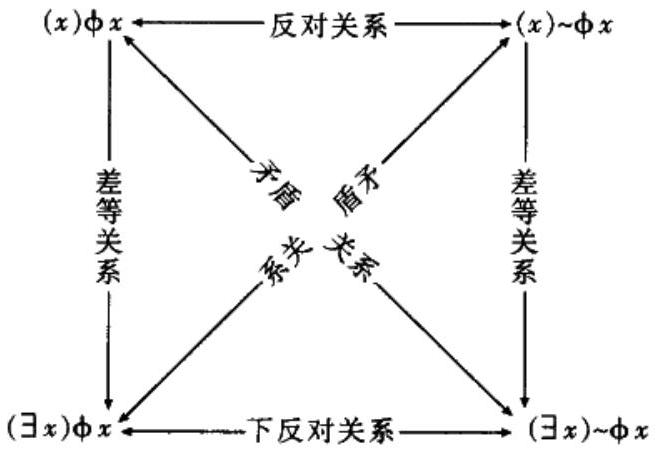
\includegraphics[max width=\textwidth, center]{2025_05_15_6a28331d5e7c993ad07ag-463}

图10—1\\
继续假定至少存在一个个体,就该方阵我们可以说:\\
1.顶端的两个命题是反对关系;就是说,它们可以同时为假,但不能同时为真。

2.底端的两个命题是下反对关系;就是说,它们可以同时为真,但不能同时为假。

3.对角线相反两端的命题是矛盾关系;它们中一个为真,则另一个必定为假。

4.在方阵的每侧,下面命题的真被它正上方命题的真所蕴涵。 
\section{传统主——谓命题}

\begin{quotation}
本节探讨传统逻辑中的四种主谓命题形式及其符号化表示。通过分析全称肯定、全称否定、特称肯定和特称否定命题的结构,我们将学习如何用量词和命题函项准确表达它们,并理解这些命题形式之间的逻辑关系,从而增强对自然语言与符号逻辑之间转换的理解。
\end{quotation}

\subsection{四种基本命题形式}

运用存在和全称量词,以及根据对图 10-1 中对当方阵的理解,我们现在开始分析(并且在推理中准确地使用)以下四种为传统逻辑研究所注重的普遍命题。这四种命题的标准例子如下:

\begin{center}
\begin{tabular}{ll}
所有人是有死的。 & [全称肯定:A] \\
所有人都不是有死的。 & [全称否定:E] \\
有些人是有死的。 & [特称肯定:I] \\
有些人不是有死的。 & [特称否定:O] \\
\end{tabular}
\end{center}

每种命题通常由其字母来指称:两种肯定命题用 A 和 I(来自拉丁文\\
affirmo,我肯定);两种否定命题用 E 和 O (来自拉丁文 nego,我否认)。\cite{peirce1883}

\subsection{A型命题的符号化}

用量词符号化这些命题,使得我们进一步扩大了命题函项概念。首先来看 \textbf{A命题}"所有人是有死的",我们从下述命题开始逐次解释:

给定不管任何事物,如果它是人,它是有死的。

其中关系代词"它"的两次出现显然是回指它们共同的先行词"事物"。与上节的前部分一样,因为它们有同样的(不确定的)指称,从而都能用字母"$x$"替换。于是该命题可改写成:

给定任何 $x$ ,如果 $x$ 是人,那么 $x$ 是有死的。

现在,用先前引入的"如果一那么"的符号,可以把前一个命题改写成:

给定任何 $x, x$ 是人 $\supset x$ 是有死的。

最后,用我们已掌握的命题函项符号和量词,原来的 A 命题可表示为:

$$
(x)(H x \supset M x)
$$

在我们的符号翻译中, A 命题是以一种新的命题函项的全称量化形式出现的。表述式 $H x \supset M x$ 是一个命题函项,它既没有单称肯定命题又没有单称否定命题作为其代人例,而是以条件陈述作为代人例,这些条件陈述的前件和后件是具有同样主项的单称命题。命题函项 $H x \supset M x$ 的代人例有条件陈述 $H a \supset M a 、 H b \supset M b 、 H c \supset M c 、 H d \supset$ $M d$ 等等。

另一些命题函项则以有同样主项的单称命题的合取为代入例。例如, $H a \cdot M a 、 H b \cdot M b 、 H c \cdot M c 、 H d \cdot M d$ 等等都是命题函项 $H x \cdot M x$ 的代人例。还有一些形如 $W x \vee B x$ 的命题函项,它们的代入例是诸如 $W a \vee$ $B a$ 和 $W b \vee B b$ 这样的析取式。实际上,任何以具有相同主项的单称命题为分支陈述的真值函项复合命题,都可以看做由某些或所有真值函项联结词(圆点号、楔劈号、马蹄号、三杠等值号和波浪号)加之简单谓词\\
( $A x 、 B x 、 C x 、 D x \cdots \cdots$ )所构成的命题函项的代人例。在把 A 命题翻译成( x )( $H \mathrm{x} \supset M x$ )时,圆括号充当标点符号,用以表明全称量词( $x$ ) "作用于"整个(复合)命题函项 $H x \supset M x$ ,或命题函项 $H x \supset M x$"作为其辖域"。

在继续讨论直言命题的其他传统形式之前,应该注意符号公式( $x$ ) ( $H x \supset M x$ )不仅是对标准形式的命题"所有 $H$'s 都是 $M$'s"的翻译,而且是对任何一个有同样含义的自然语言句子的翻译。\cite{brown1954} 在自然语言中,述说这同一件事有许多不同的方式。它们的部分清单如下:"$H$ 是 $M$","一个 $H$ 就是一个 $M$","每个 $H$ 是 $M$","每一个 $H$ 是 $M$","任何 $H$ 是 $M$", "没有 $H$ 不是 $M$","是 $H$ 的每个事物都是 $M$","是 $H$ 的任何事物都是 $M "$ ,"如果任何事物是 $H$ ,那么它是 $M$","如果某事物是 $H$ ,那么它是 $M$","是 $H$ 的无论什么东西都是 $M$","$H$'$s$ 全都是 $M$'$s$","只有 $M$'$s$ 是 $H^{\prime} s "$ ,"除了 $M^{\prime} s$ 以外,没什么是 $H^{\prime} s "$ ,"没什么是 $H$ ,除非它是 $M^{\prime}$",以及"没有什么是 $H$ 但不是 $M$"。再者,同一含义的命题可以用抽象名词表达:"人蕴涵(或涵衍)有死"可以正确地符号化为一个 A 命题。符号逻辑语言对相当数量的自然语言句子的共同含义有一个单一的表达式,这一点被认为是符号逻辑在认知或信息方面比自然语言优越之处,一一尽管从修辞力或诗意表现的观点看,我们承认这是一种劣势。 

\subsection{其他类型命题的符号化}

\textbf{E命题}"所有人都不是有死的"可以被依次释为:

\begin{quote}
给定不管任何个体事物,如果它是人,那么它不是有死的。\\
给定任何 $x$ ,如果 $x$ 是人,那么 $x$ 不是有死的。\\
给定任何 $x, x$ 是人 $\supset x$ 不是有死的。
\end{quote}

最后可以释为:

$$
(x)(H x \supset \sim M x)
$$

这种符号翻译不仅表示了自然语言中传统的 E 形式,同样也表示了一些说同一件事的不同方式,如"没有是 $M$ 的 $H$","没有什么既是 $H$ 又是 $M$",以及"$H$ 从不是 $M$"。

同样,\textbf{I命题}"有些人是有死的"可以依次释为:

至少有一个是人且有死的事物。\\
至少有这样一个 $x, x$ 是人并且 $x$ 是有死的。\\
至少有这样一个 $x, x$ 是人• $x$ 是有死的。

进而可以释为:

$$
[(\exists x)(H x \cdot M x)]
$$

最后,\textbf{O命题}"有些人不是有死的"可以依次释为:

至少存在一个是人但不是有死的事物。\\
至少存在这样一个 $x, x$ 是人并且 $x$ 不是有死的。\\
至少存在这样一个 $x, x$ 是人• $\sim x$ 是有死的。

它可以完全符号化为:

$$
[(\exists x)(H x \cdot \sim M x)]
$$

\subsection{命题形式间的逻辑关系}

若用希腊字母 phi( $\phi$ )和 psi( $\Psi$ )表示任何一个谓词,传统逻辑的四个主—谓型普遍命题可以在图 10—2 所示的方阵中得到表达。\\
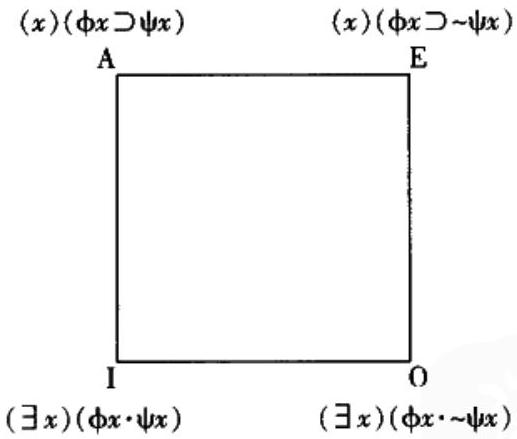
\includegraphics[width=\textwidth]{images/2025_05_15_6a28331d5e7c993ad07ag-466.jpg}

图10-2\\
显然, A 命题和 O 命题是\textbf{矛盾关系},一个是另一个的否定; E 命题和 I 命题也是矛盾关系。

有人可能会认为,一个 I 命题可以从与之相对的 A 命题推出,一个 O命题可以从与之相对的 E 命题推出,但情况并非如此。一个 A 命题为真时,与之对应的 I 命题却可能是假的。如果 $\phi_{x}$ 是一个没有真代人例的命

题函项,那么,不管命题函项 $\Psi x$ 有何种代人例,(复合)命题函项 $\phi_{x} \supset$ $\Psi x$ 的全称量化式都是真的。例如,考虑命题函项"$x$ 是一个人首马身的怪物",我们把它简写为 $C x$ 。因为不存在人首马身的怪物,$C x$ 的每个代入例都是假的,即 $C a 、 C b 、 C c \cdots \cdots$ 都为假。因此,复合命题函项 $C x \supset B x$的每个代人例都是一个前件为假的条件陈述。这样,其代人例 $\mathrm{Ca} \supset \mathrm{Ba}$ 、 $C b \supset B b 、 C c \supset B c$ 都是真的,因为任何一个断言实质蕴涵的条件陈述,如果其前件为假,那么它必定为真。由于其所有代人例都是真的,所以,命题函项 $C x \supset B x$ 的全称量化式为真,即 A 命题 $(x)(C x \supset B x)$ 为真。但与之相对的 I 命题 $(\exists x)(C x \cdot B x)$ 却是假的,因为命题函项 $C x \cdot B x$没有真代人例。 $C x \cdot B x$ 没有真代人例可以从 $C x$ 没有真代人例推出。 $C x \cdot B x$ 的各个代人例,如 $C a \cdot B a 、 C b \cdot B b 、 C c \cdot B c \cdots \cdots$ 都是第一个合取支为假的合取式,因为 $C a 、 C b 、 C c \cdots \cdots$ 都为假。由于其所有代人例都为假,所以命题函项 $C x \cdot B x$ 的存在量化式为假,即 I 命题( $\exists x$ )( $C x \cdot B x$ )为假。因此,有可能一个 A 命题是真的,而与之对应的 I 命题却是假的。

这种分析还可表明,为什么有可能一个 E 命题是真的,而与之对应的 $O$ 命题却是假的。如果我们以命题函项 $\sim B x$ 替换前面讨论中的命题函项 $B x$ ,那么,$(x)(C x \supset \sim B x)$ 可以是真的,而 $(\exists x)(C x \cdot \sim B x)$ 却是假的。当然,这也是因为并没有人首马身的怪物。

\subsection{命题类型间的关键区别}

问题的关键在于:A 命题和 E 命题并不断言或假定任何事物存在,它们仅断言情况是这样的:如果有某事,则有另外一件事。但 I 命题和 O 命题却假定某物存在,它们断言情形是这样的:有这件事并且有另一件事。 1 命题和 $O$ 命题中的\textbf{存在量词}是区别的关键所在。从一个并不断言或假定任何事物存在的命题推出某物的存在,这显然是错误的。

如果我们假定至少有一个个体存在,那么( $x$ )( $C x \supset B x$ )确实蕴涵 ( $\exists x) ~(C x \supset B x)$ 。但后者不是一个 I 命题。 I 命题"有些人首马身的怪物是漂亮的"应符号化为 $(\exists x)(C x \cdot B x)$ ,它说的是,至少存在一个漂亮的人首马身的怪物。但在自然语言中,被符号化为( $\exists x$ )( $C x \supset B x$ )的东西,可以被理解为"至少存在一个如此这般的事物,如果它是人首马身的怪物,那么它是漂亮的"。它并没说存在一个人首马身的怪物,而只是说存在一个个体,它或者不是人首马身的怪物,或者是漂亮的。而这个命题只在两种情况下是假的:第一,如果根本不存在个体;第二,如果所有个体都是人首马身的怪物,并且它们当中没有一个是漂亮的。通过作这样

一个明确的(并且显然是真的)假定,即假定宇宙中至少存在一个个体,我们可以排除第一种情形。第二种情形是如此极端地不合理,以致与 I 形命题( $\exists x$ )( $\phi_{x} \cdot \Psi x$ )的重要性相反,任何形如( $\exists x$ )( $\phi_{x} \supset \Psi x$ )的命题都必定是非常平庸的。显而易见,尽管在自然语言中 A 命题"所有人是有死的"和 I 命题"有些人是有死的"的区别,仅在于初始词"所有"和"有些"的不同,但它们意义上的区别并不限于全称量化和存在量化,而是比这深刻得多。经量化而产生 A 命题和 I 命题的命题函项不仅在量化上有区别,而且它们还是不同的命题函项,一个含有"$\supset$",另一个含有"•"。换言之,A 命题和 I 命题并不像它们在自然语言中看起来那么相似。它们之间的区别可通过使用命题函项符号和量词符号得以彰显。

\subsection{命题变形技巧}

就逻辑操作来说,处理那些否定号的出现——如果有否定号出现的话——只作用于简单谓述的公式最为方便。因此,我们将在必要时通过替换来得到这种公式。要做到这一点很简单。从第9章所确立的推论规则可知,我们可以用另一个与之逻辑等价的表述式来替换一个表述式。而我们有四个这样的逻辑等价式(10.2节),它们当中否定号在量词之前的命题,都与另一个否定号直接作用于简单谓述的命题等价。用我们熟悉已久的推论规则,可以移动否定号,使它们最终不再作用于复合表达式,而只作用于简单谓述。譬如说,公式:

$$
\sim(\exists x)(F x \cdot \sim G x)
$$

可以依次改写。首先,如果我们用 10.2 节所给的第三个逻辑等价式,它可以变形为:

$$
(x) \sim(F x \cdot \sim G x)
$$

然后,可运用德摩根律使之变成:

$$
(x)(\sim F x \vee \sim \sim G x)
$$

再用双重否定律可得公式:

$$
(x)(\sim F x \vee G x)
$$

最后,若援引实质蕴涵定义,原公式也可以改写成下述 A 命题:

$$
(x)(F x \supset G x)
$$

在转到关于非复合陈述推论的话题之前,读者应该进行一些把非复合陈述从自然语言翻译成逻辑符号的训练。自然语言有如此之多不规则的和惯用的构造,以致不可能有把自然语言语句翻译成逻辑符号的简单规则。在任何情形下都要先理解语句的含义,然后用命题函项和量词术语予以重述。

\begin{center}
\fbox{\parbox{0.95\textwidth}{
\textbf{本节要点}
\begin{itemize}
\item \textbf{传统四种命题形式}:
  \begin{itemize}
  \item A型(全称肯定):所有S是P,符号化为(x)(Sx⊃Px)
  \item E型(全称否定):所有S都不是P,符号化为(x)(Sx⊃~Px)
  \item I型(特称肯定):有些S是P,符号化为(∃x)(Sx·Px)
  \item O型(特称否定):有些S不是P,符号化为(∃x)(Sx·~Px)
  \end{itemize}
\item \textbf{符号化的结构差异}:
  \begin{itemize}
  \item A型和E型命题使用条件结构(⊃)和全称量词
  \item I型和O型命题使用合取结构(·)和存在量词
  \item 这种结构差异揭示了自然语言中隐含的逻辑区别
  \end{itemize}
\item \textbf{命题间的逻辑关系}:
  \begin{itemize}
  \item A与O、E与I构成矛盾关系(一真一假)
  \item A命题不必然蕴涵I命题(当主词类为空时)
  \item E命题不必然蕴涵O命题(当主词类为空时)
  \end{itemize}
\item \textbf{存在假定的区别}:
  \begin{itemize}
  \item A型和E型命题不假定主词类存在
  \item I型和O型命题假定主词类有实例存在
  \item 这一区别解释了为何A型命题不必然蕴涵I型命题
  \end{itemize}
\end{itemize}
}}
\end{center}

\section{有效性证明}

\begin{quotation}
本节讨论如何证明那些有效性取决于非复合陈述内在结构的论证。我们将介绍四个新的推论规则:全称列举、全称概括、存在列举和存在概括,通过这些规则,我们能够构造出涉及量化命题的形式证明,从而扩展我们的逻辑分析工具,使之能够处理更复杂的论证形式。
\end{quotation}

\subsection{扩充推论规则}

某些论证的有效性取决于在其中出现的非复合陈述的内在结构,为了构造它们有效性的形式证明,我们必须进一步扩充推论规则表。只需增加四个规则,我们将在涉及必须使用它们的那些论证时逐次引人。

考虑本章所引的第一个论证:"所有人都是有死的。苏格拉底是人。因此,苏格拉底是有死的。"可以符号化为:

$$
(x)(H x \supset M x)
$$

Hs\\
$\therefore M s$\\
第一个前提断定了命题函项 $H x \supset M x$ 的全称量化式。由于一个命题函项的全称量化式为真,当且仅当它的所有代人例都为真,从第一个前提可以推出命题函项 $H x \supset M x$ 的任何一个我们需要的代人例。此处即可以推出代人例 $H s \supset M s$ 。从它和第二个前提 $H s$ ,根据肯定前件式,可以直接得出结论 $M s$ 。

如果给我们的推论规则表加上这样一个原则,即一个命题函项的任一代入例都可以有效地从其全称量化式推得,那么,依照扩充了的基本有效论证形式表,我们可以给出该论证之有效性的形式证明。这种新的推论规则就是\textbf{全称列举原则},简写为"UI"。用希腊字母 $n u(v)$ 表示任一个体符号,我们可以把该新规则表述为:

$$
\begin{aligned}
& \mathrm{UI}:(x)(\phi x) \\
& \quad \therefore \phi v \quad(v \text { 是任一个体符号 })
\end{aligned}
$$

其有效性的形式证明现在可以写成:

\begin{center}
\begin{tabular}{ll}
1.$(x)(H x \supset M x)$ &  \\
2.$H s$ &  \\
 & $\therefore M s$ \\
3.$H s \supset M s$ & $1, \mathrm{UI}$ \\
4.$M s$ & $3,2, \mathrm{M} . \mathrm{P}$. \\
\end{tabular}
\end{center}

\subsection{全称概括原则}

增加 UI 大大地强化了我们的证明工具,但我们还需要更多的规则。需要另一些支配量化的规则,这种需要是和这样的论证相联系的,如"所有人都是有死的。所有希腊人都是人。因此所有希腊人都是有死的。"这个论证的符号翻译是:

$$
\begin{aligned}
& (x)(H x \supset M x) \\
& (x)(G x \supset H x) \\
& \therefore(x)(G x \supset M x)
\end{aligned}
$$

其中,前提和结论都是普遍命题而不是单称命题,是命题函项的全称量化式而不是其代人例。根据 UI,我们可以有效地从这两个前提推出下述条件陈述对子:

$$
\begin{array}{lllll}
G a \supset H a & G b \supset H b & G c \supset H c & G d \supset H d & \\
H a \supset M a & H b \supset M b & H c \supset M c & H d \supset M d & \ldots \ldots
\end{array}
$$

通过连续使用假言三段论规则,我们可以有效地推出结论:

$$
G a \supset M a, \quad G b \supset M b, \quad G c \supset M c, \quad G d \supset M d \quad \ldots \ldots
$$

如果 $a, b, c, d \cdots \cdots$ 是所有存在的个体,那么,我们从前提的真就可以有效地推出命题函项 $G x \supset M x$ 的所有代人例的真。由于一个命题函项的全称量化式为真,当且仅当,它的所有代人例都为真,我们可以继续推出 ( $x$ )( $G x \supset M x$ )为真,而它就是该论证的结论。

前面一段可以看做构成了上述论证有效性的一个非形式的证明,在证明中运用了假言三段论规则和支配量化的两个规则。它描述了一个长度不确定的陈述序列:前提中两个被全称量化的命题函项的所有代人例的序列,以及其全称量化式是结论的那个命题函项的所有代人例的序列。一个形式证明不能包含这样的不确定的甚或无限长的陈述序列。因此,必须寻求某种方法,它能以某种有限的、确定的方式来表达这些长度不确定的序列。

基础数学的一个一般技巧为做到这一点提供了提示。一个试图证明所有三角形都具有某种属性的几何学者,可以从"令 $A B C$ 是一个任意选取的三角形"出发。然后对三角形 $A B C$ 进行推理,确立它具有被探究的那种属性,由此可得出结论,所有三角形具有该属性。是什么东西能为他的最后结论进行辩护呢?承认这个特定的三角形 $A B C$ 有该属性,为什么可以得出所有的三角形都有这种属性?答案很容易见得:如果除了假定它是三角形外,我们对三角形 $A B C$ 没作任何其他假定,那么,符号"$A B C$"可以被看做是指称你所挑选的任何三角形。几何学者的论证确立了任一三角形具有所探究的属性,而如果任一三角形都具有某属性,那么所有的三角形都具有该属性。我们现在也可引进一个符号,它类似于几何学者所谈论的"一任意选取的三角形 $A B C$"。这使我们可以谈论某命题函项的任一代人例,而不用去罗列其不确定的或无限数量的代人例。

我们将用(迄今还没用过)小写字母 $y$ 来指称一任意选取的个体,以一种类似于几何学者使用字母 $A B C$ 的方式来使用它。由于从一个命题函项的全称量化式可以推出它的任一代人例,故亦可推出以 $y$ 替换 $x$ 所得到的那个代人例。在此,$y$ 指称"一任意选取的个体"。这样,我们可以着手进行上述论证有效性的形式证明:

1.$(x)(H x \supset M x)$\\
2.$(x)(G x \supset H x)$

$$
\therefore(x)(G x \supset M x)
$$

\begin{center}
\begin{tabular}{ll}
3.$H y \supset M y$ & 1, UI \\
4.$G y \supset H y$ & 2, UI \\
5.$G y \supset M y$ & 4,3, H.S. \\
\end{tabular}
\end{center}

我们从前提演绎出了陈述 $G y \supset M y$ ,由于 $y$ 指称"一任意选取的个体",所以,该陈述实际上是断言命题函项 $G x \supset M x$ 的任一代人例为真。既然任一代人例为真,所有的代人例必定为真,因此,该命题函项的全称量化也必是真的。我们可以把这个原则加到推论规则表中,表述如下:从一个

命题函项关于任意选取的个体名称的代入例,我们可以有效地推出该命题函项的全称量化式。这个规则允许我们进行概括,也就是从一个特定的代人例进到一个概括的或全称量化的表述式,故称为\textbf{全称概括原则},并缩写为"UG"。它被表述成:

$$
\begin{aligned}
\mathrm{UG}: & \phi_{y} \\
\therefore(x)\left(\phi_{x}\right) & (y \text { 指称"一任意选取的个体") }
\end{aligned}
$$

前面的形式证明的第六行即最后一行,现在就可以写(并被证明)为:\\
6.$(x)(G x \supset M x)$\\
5,UG

我们来回顾一下前面的讨论。在几何学者的证明中,对 ABC 所作的唯一假定就是它是一个三角形,因此,被证明为对 ABC 为真的东西也就被证明为对任一三角形为真。在我们的证明中,对 $y$ 所作的唯一假定是它是一个个体词,因此,被证明为对 $y$ 为真的东西也就被证明为对任一个体为真。符号 $y$ 是一个个体符号,但它是一个很特殊的个体符号。特别是通过使用 UI,它被引人到证明中,并且只有当出现了 $y$ 时才允许使用UG。

以下是另一个有效论证,它的有效性的证明要求使用 UG 和 UI:"没有人是完美的。所有希腊人都是人。因此没有希腊人是完美的。"\cite{kneale1962} 它的有效性的形式证明是:

1.$(x)(H x \supset \sim P x)$\\
2.$(x)(G x \supset H x)$

$$
\therefore(x)(G x \supset \sim P x)
$$

3. $\mathrm{H} y \supset \sim \mathrm{P} y \quad 1$ ,UI\\
4.GyつHy 2,UI\\
5.Gyコ~Py 4,3,H.S.\\

6.$(x)(G x \supset \sim P x) \quad$ 5,UG\\
上面的证明看起来多少有点不自然,需要我们对 $(x)\left(\phi_{x}\right)$ 和 $\phi_{y}$ 做出仔细的区分。说它们尽管不同但根据 UG 和 UI 又必定可以相互推出,似乎二者之间没有实质差别。但它们之间确实有一种形式的差别。陈述 ( $x$ )( $H x \supset M x$ )是一个非复合陈述,而 $H y \supset M y$ 作为一个条件陈述,是一个复合陈述。依照原先含有 19 个规则的推论规则表,从两个非复合陈述 $(x)(G x \supset H x)$ 和 $(x)(H x \supset M x)$ 出发,我们不能作相关的推理。

但从复合陈述 $G y \supset H y$ 和 $H y \supset M y$ 出发,根据假言三段论,就可以得出所要的结论 $G y \supset M y$ 。规则 $U I$ 用来从非复合陈述得出复合陈述,我们先前的推论规则无法施于非复合陈述,但可以施于复合陈述以得出想要的结论。因此,量化规则增加了我们的逻辑工具,使得我们能够证明本质地涉及非复合(概括的)命题的论证的有效性,以及前一些章节所讨论的另一类(更简单的)论证的有效性。另一方面,尽管有这种形式的差别,( $x$ ) ( $\phi_{x}$ )和 $\phi_{y}$ 必定是逻辑等价的,否则,规则 UG 和 UI 就不是有效的。对依据推论规则表来证明论证的有效性来说,这种差别和逻辑等价都很重要。把 UG 和 UI 加到推论规则表中使之得到了很大强化。

\subsection{存在量化规则}

当我们转向涉及存在命题的论证时,推论规则表必须进一步扩充。我们可从这样一个很便捷的例子着手:"所有罪犯都是邪恶的。有些人是罪犯。因此有些人是邪恶的。"它可以符号化为:

$$
\begin{aligned}
& (x)(C x \supset V x) \\
& (\exists x)(H x \cdot C x) \\
& \therefore(\exists x)(H x \cdot V x)
\end{aligned}
$$

一个命题函项的存在量化式为真,当且仅当,它至少有一个真代人例。因此,无论 $\phi$ 指谓何种属性,( $\exists x$ )( $\phi_{x}$ )所说的就是,至少存在一个具有属性 $\phi$ 的个体。如果一个个体常元(除了特定的符号 $y$ )在早先的上下文中没有使用过,我们可以用它来指称具有属性 $\phi$ 的那个个体,或者,如果有几个具有属性 $\phi$ 的个体,用它指称其中的某一个。若知道存在这样一个个体,臂如 $a$ ,我们就知道 $\phi_{a}$ 是命题函项 $\phi_{x}$ 的一个真代人例。故我们给推论规则表加上这样一个规则:从一个命题函项的存在量化式,可以推得关于在其语境中早先没有出现过的任一个体常元(除 $y$ 之外)的代入例。这个新推论规则叫\textbf{存在列举原则},可缩写为"EI"。它可以表述成:

$$
\mathrm{EI}:(\exists x)\left(\phi_{x}\right)
$$

$\therefore \phi U \quad[U$ 是任一在语境中先前没有出现过的个体常元(除 $y$之外)〕

如果确认所添加的推理规则 EI,我们即可着手证明上述论证的有效性:

1.$(x)(C x \supset V x)$

2.$(\exists x)(H x \cdot C x)$

$$
\therefore(\exists x)(H x \cdot V x)
$$

3. $\mathrm{Ha} \cdot \mathrm{Ca}$ 2,EI\\
4. $\mathrm{Ca} \supset \mathrm{Va} \quad 1$ ,UI\\
5. $\mathrm{Ca} \cdot \mathrm{Ha}$ 3,Com.\\
6. Ca 5,Simp.\\
7.Va 4,6,M.P.\\
8. Ha 3 ,Simp.\\
9. $\mathrm{Ha \cdot Va} \quad 8,7$, Conj.\\
到目前为止,我们演绎出了 $\mathrm{Ha} \cdot \mathrm{Va}$ ,它是其存在量化式被结论所断定的那个命题函项的代人例。由于一个命题函项的存在量化式为真,当且仅当,它至少有一个为真的代人例,我们为推论规则表再增加这样一个规则:从一个命题函项的任一为真的代入例,我们可以有效地推出该命题函项的存在量化式。这第四个也是最后一个推论规则叫\textbf{存在概括原则},缩写为"EG",它可以表述为:

$$
\begin{gathered}
\text { EG: } \phi_{v} \quad(v \text { 是任一个体符号) } \\
\therefore(\exists x)\left(\phi_{x}\right)
\end{gathered}
$$

前面开始的那个证明的第十行也即最后一行,现在可以写(并且被证明)为:

$$
\text { 10. }(\exists x)(H x \cdot V x) \quad 9, \mathrm{EG}
$$

\subsection{使用限制}

对 EI 的使用必须施加必要的限制,这一点可以通过考察如下明显无效的论证看出来:"有些短伆鳄被关在笼子里。有些鸟被关在笼子里。因此有些短吻鳄是鸟。"如果我们不对 EI 施加这样一种限制——根据 EI 从一个命题函项的存在量化式推出的代人例,只能含有一个在语境中早先没出现过的个体符号(除 $y$ 之外),那么,我们就可以构造出这个无效论证的有效性"证明"。这样一个错误的"证明"可以如下进行:

1.$(\exists x)(A x \cdot C x)$\\
2.$(\exists x)(B x \cdot C x)$

$$
\therefore(\exists x)(A x \cdot B x)
$$

4. $\mathrm{Ba} \cdot \mathrm{Ca}$\\
5.$A a$\\
6.$B a$\\
7.$A a \cdot B a$\\
8.$(\exists x)(A x \cdot B x)$

2,EI(错!)\\
3,Simp.\\
4,Simp.\\
5,6,Conj.\\
7,EG

这个"证明"的错误出现在第 4 行。我们从第二个前提 $(\exists x)(B x \cdot C x)$可知,至少存在这样一个事物,它既是鸟又被关在笼子里。如果我们在第 4 行给它自由地指派一个名称 $a$ ,我们当然就可以断言 $B a \cdot C a$ 。但我们绝不能自由地指派这样一个"$a$",因为它作为一只关在笼子里的短吻鳄的名字,已经先在第 3 行中出现了。为避免这种错误,我们使用 EI 时必须服从这种必要的限制。由前面的讨论可明显见得:在任何要使用 EI 和 UI 的证明中,应该总是先使用 EI 。

对更复杂的论证模式来说,特别是那些涉及关系的论证,我们还必须对四个量化规则施加某些附加限制。但就目前这种类型的论证即传统上叫做直言三段论的论证来说,目前的限制已足以避免出错。

\subsection{四个附加推论规则总结}

下述四个规则使得我们可以把非复合的、概括的命题转化为与其等值的复合命题,第 9 章所列的那 19 个推论规则适用于这些复合命题。它们还使我们可以把复合命题转化为等值的非复合命题。因此,这四个附加规则使得构造某些论证的有效性的形式证明成为可能,这些论证的有效性取决于它们所包含的一些非复合陈述的内在结构。这四个附加规则如下:

\paragraph{1.全称列举}
UI:$(x)(\phi x), \therefore \phi \cup$(在此,$v$ 是任一个体符号)\\
这个规则大体上说的是:一个命题函项的任何代入例都可以从它的全称量化式推出。

\paragraph{2.全称概括}
UG:$\phi_{y}, \therefore(x)\left(\phi_{x}\right)$(在此,$y$ 指称"一任意选取的个体")\\
这个规则大体上说的是:从一个命题函项关于一任意选取的个体名称的代入例,我们可以有效地推出该命题函项的全称量化式。

\paragraph{3.存在列举}
EI:$(\exists \mathrm{x})\left(\phi_{\mathrm{x}}\right), \therefore \phi_{\mathrm{u}}$[在此,$v$ 是任一在上下文中先前没有出现

过的个体常元(除了 y)〕\\
这个规则大体上说的是:从一个命题函项的存在量化式,我们可以推出,它关于早先上下文的任何地方都没出现的任一个体常元(除了 $y) ~$ 的代入例为真。

\paragraph{4.存在概括}
EG:$\phi_{v}, \therefore(\exists x)\left(\phi_{x}\right)$(在此,$v$ 是任一个体符号)\\
这个规则大体上说的是:从一个命题函项的任一为真的代入例,我们可以有效地推出该命题函项的存在量化式。 

\begin{center}
\fbox{\parbox{0.95\textwidth}{
\textbf{本节要点}
\begin{itemize}
\item \textbf{四个量化推论规则}:
  \begin{itemize}
  \item 全称列举(UI):从(x)(φx)推出φv
  \item 全称概括(UG):从φy推出(x)(φx)
  \item 存在列举(EI):从(∃x)(φx)推出φv
  \item 存在概括(EG):从φv推出(∃x)(φx)
  \end{itemize}
\item \textbf{规则使用的重要限制}:
  \begin{itemize}
  \item UG规则中,y必须是"任意选取的个体"
  \item EI规则中,v必须是先前未使用过的个体符号
  \item 在证明中应先使用EI再使用UI
  \item 这些限制避免了错误的推论
  \end{itemize}
\item \textbf{规则的功能和意义}:
  \begin{itemize}
  \item 使我们能够在非复合陈述和复合陈述间转换
  \item 使已有的19个推论规则能够应用于量化表达式
  \item 扩展了我们处理更复杂论证形式的能力
  \item 使我们能够形式化地证明直言三段论的有效性
  \end{itemize}
\item \textbf{规则的应用}:
  \begin{itemize}
  \item 可以处理类似"所有S是M,所有P是S,因此所有P是M"的传统三段论
  \item 可以证明包含存在命题的论证的有效性
  \item 为分析非复合陈述的内在结构提供了必要工具
  \end{itemize}
\end{itemize}
}}
\end{center} 
\section{无效性证明}

\begin{quotation}
本节讨论如何证明涉及量词的论证的无效性。通过引入特定的模型和真值指派方法,我们可以系统性地处理含有量化命题的论证,并确定它们是否无效。相比于简单的逻辑类比,这种方法提供了更加严格和普遍的无效性证明技术。
\end{quotation}

\subsection{逻辑类比的局限性}

要证明一个涉及量词的论证无效,我们可以用逻辑类推进行反驳的方法。例如:"所有保守派都是行政机关的反对者;有些代表是行政机关的反对者;因此,有些代表是保守派。"这个论证可以通过这样一个逻辑类推被证明为无效,即"所有猫都是动物;有些狗是动物;因此,有些狗是猫"。这个论证显然无效,因为已知它的前提为真而结论为假。但这种类比并非总是很容易构造。因此,需要某种更有力的证明无效性的方法。

\subsection{真值指派方法的扩展}

在前一章中,我们详述了一种证明涉及真值函项复合陈述的论证之无效性的方法。这种方法是通过对论证中的简单分支陈述进行真值指派,使得论证的前提为真而结论为假。我们可以设法使这种方法适用于使用量词的论证。这涉及这样一个一般假定,即至少存在一个个体。若一个涉及量词的论证有效,那么,只要至少有一个个体存在,这个论证的前提为真而结论为假就必定是不可能的。

\subsection{有限域模型中的量化}

如果恰好存在一个个体,两个个体,三个个体……那么,至少存在一个个体这个一般假定就得到了满足。如果作了任何这样一个关于个体的确切数量的假定,就有一个关于普遍命题与单称命题的真值函项复合式的等价式。如果刚好存在一个个体,譬如说 $a$ ,那么:

$$
(x)\left(\phi_{\mathrm{x}}\right) \stackrel{\mathrm{T}}{=} \phi_{a} \stackrel{\mathrm{T}}{=}(\exists x)\left(\phi_{x}\right)
$$

如果刚好存在两个个体,臂如说 $a$ 和 $b$ ,那么:

$$
(x)\left(\phi_{x}\right) \stackrel{\mathrm{T}}{\equiv}\left[\phi_{a} \cdot \phi_{b}\right] \text {, 而 }(\exists x)\left(\phi_{x}\right) \stackrel{\mathrm{T}}{\equiv}\left[\phi_{a} \vee \phi_{b}\right]
$$

如果刚好存在三个个体,譬如说 $a 、 b$ 和 $c$ ,那么:

$$
(x)\left(\phi_{x}\right) \stackrel{\mathrm{T}}{=}\left[\phi_{a} \cdot \phi_{b} \cdot \phi_{c}\right] \text {, 而 }(\exists x)\left(\phi_{x}\right) \stackrel{\mathrm{T}}{=}\left[\phi_{a} \vee \phi_{b} \vee \phi_{c}\right]
$$

一般的,如果刚好存在 $n$ 个个体,譬如说 $a 、 b 、 c \cdots \cdots n$ ,那么:

$$
\begin{aligned}
& (x)\left(\phi_{x}\right) \stackrel{\mathrm{T}}{=}\left[\phi_{a} \cdot \phi_{b} \cdot \phi_{c} \cdots \cdot \phi_{n}\right] \\
& \text { 而 }(\exists x)\left(\phi_{x}\right) \cong\left[\phi_{a} \vee \phi_{b} \vee \phi_{c} \vee \cdots \vee \phi_{n}\right]
\end{aligned}
$$

由于它们是我们关于全称和存在量词定义的推论,所以这些双条件陈述为真。这里并没有用到前一节所阐释的四个量化规则。

\subsection{使用模型证明无效性}

一个涉及量词的论证有效,当且仅当,不管存在多少个体它都是有效的,一一假定至少存在一个个体的话。因此,如果存在一个至少含有一个个体的可能域或\textbf{模型},它使得某论证相对该模型来说,其前提为真而结论为假,那么,这样一个涉及量词的论证就被证明为无效。考察论证:"所有雇佣兵都是不可靠的。没有游击队员是雇佣兵。因此没有游击队员是不可靠的。"它可以符号化为:

$$
\begin{aligned}
& (x)(M x \supset U x) \\
& (x)(G x \supset \sim M x) \\
& \therefore(x)(G x \supset \sim U x)
\end{aligned}
$$

如果刚好存在一个个体,譬如说 $a$ ,这个论证逻辑地等价于:

$$
\begin{aligned}
& M a \supset U a \\
& G a \supset \sim M a \\
& \therefore G a \supset \sim U a
\end{aligned}
$$

给 $G a$ 和 $U a$ 指派真值真,给 Ma 指派真值假,即可以证明上式是无效的。 (这种真值指派是一种简略的描述方式,它把所讨论的模型描述成只含有一个个体 $a$ ,这个个体是游击队员且不可靠,但不是雇佣兵。)于是,原来的论证对于一个只含有一个个体的模型来说不是有效的,因此它是无效的。类似的,通过描述只含有一个个体 $a$ 的模型,使得 $A a$ 和 $D a$ 被赋值为真,且 $C a$ 被赋值为假,我们就可以证明本节提到的第一个论证的无效性。\cite{tarski1954}

\subsection{逐渐扩大模型的方法}

有些论证对于刚好只有一个个体的模型来说是有效的,但对于有两个或更多个体的模型来说则不然。譬如:

$$
\begin{aligned}
& (\exists x) F x \\
& \therefore(x) F x
\end{aligned}
$$

这样的论证必须被当做是无效的,因为只要至少存在一个个体,那么,一个有效的论证就必定有效而不管存在多少个体。这种论证的另一个例子是:"所有牧羊犬都是可爱的。有些牧羊犬是看门狗。因此,所有看门狗都是可爱的。"它的符号翻译是:

$$
\begin{aligned}
& (x)(C x \supset A x) \\
& (\exists x)(C x \cdot W x) \\
& \therefore(x)(W x \supset A x)
\end{aligned}
$$

对一个刚好只有一个个体 $a$ 的模型来说,该论证逻辑地等价于:

$$
\begin{aligned}
& C a \supset A a \\
& C a \cdot W a \\
& \therefore W a \supset A a
\end{aligned}
$$

这个论证是有效的。但对一个有两个个体譬如 $a$ 和 $b$ 的模型来说,它逻辑地等价于:

$$
\begin{aligned}
& (C a \supset A a) \cdot(C b \supset A b) \\
& (C a \cdot W a) \vee(C b \cdot W b) \\
& \therefore(W a \supset A a) \cdot(W b \supset A b)
\end{aligned}
$$

通过对 $C a 、 A a 、 W a 、 W b$ 指派真,对 $C b 、 A b$ 指派假,可以证明该论证无效。于是,原论证对一个刚好有两个个体的模型来说不是有效的,因此它是无效的。对任何这种一般类型的无效论证来说,有可能描述一个含有有限数量个体的模型,用真值指派的方法可以证明,与这个论证逻辑等价的真值函项论证相对于该模型是无效的。

需要再次强调:在从一个涉及普遍命题的论证转化为一个真值函项论

证(相对于某特定模型,它逻辑等价于给定论证)的过程中,并没有用到我们的那四个量化规则。相反,真值函项论证的每个陈述,逻辑地等价于给定论证中与之对应的普遍命题。这种逻辑等价可以由本节中早些时候所阐述的那些双条件陈述来解释。相对于所讨论的那个模型,它们的逻辑真可以从全称量词和存在量词的定义推出。

\subsection{无效性证明的一般步骤}

证明一个含有普遍命题的论证无效的程序如下。首先,考察一个只含有一个个体 $a$ 的\textbf{一元模型}。然后,写出该论证相对于此模型的逻辑等价真值函项论证。通过把原论证的每个普遍命题(量化的命题函项)转化为该命题函项关于 $a$ 的代人例,就可以做到这一点。如果对它的简单分支陈述进行真值指派可以证明该真值函项论证无效,那么这就足以证明原论证无效。如果不能做到这一点,就接着考察一个含有两个体 $a$ 和 $b$ 的\textbf{二元模型}。为了得到相对于这个更大模型来说逻辑等价的真值函项论证,我们可以简单地把原来关于 $a$ 的每个代人例和一个关于 $b$ 的新代人例结合起来。这种"结合"必须依照前面所陈述的那些逻辑等价式。也就是说,在原论证含有一个全称量化的命题函项( $x$ )( $\phi_{x}$ )时,就用合取("•")把新的代人例 $\phi_{b}$ 和第一个代人例 $\phi_{a}$ 结合起来;在原论证含有一个存在量化的命题函项( $\exists x$ )( $\phi_{x}$ )时,就用析取(" V ")把新的代人例 $\phi_{b}$ 和第一个代入例 $\phi_{a}$ 结合起来。前述例子说明了这种程序。如果对它的简单分支陈述进行真值指派可以证明该真值函项论证无效,那么这就足以证明原论证无效。如果做不到这一点,就接着考察一个含有个体 $a 、 b$ 和 $c$ 的三元模型等等。本书中没有哪个习题要求一个含有超过三个元素的模型。 

\begin{center}
\fbox{\parbox{0.95\textwidth}{
\textbf{本节要点}
\begin{itemize}
\item \textbf{无效性证明方法}:
  \begin{itemize}
  \item 逻辑类比方法:构造结构相似但明显无效的类比论证
  \item 真值指派方法:在特定模型中找到使前提为真而结论为假的情况
  \item 模型扩展法:从一元模型开始,逐渐扩大模型规模直到找到反例
  \end{itemize}
\item \textbf{有限域中的量化等价式}:
  \begin{itemize}
  \item 一元模型:(x)(φx) ≡ φa ≡ (∃x)(φx)
  \item 二元模型:(x)(φx) ≡ [φa·φb],(∃x)(φx) ≡ [φa∨φb]
  \item 三元模型:(x)(φx) ≡ [φa·φb·φc],(∃x)(φx) ≡ [φa∨φb∨φc]
  \item 这些等价式基于量词的定义,而非推论规则
  \end{itemize}
\item \textbf{无效性的定义}:
  \begin{itemize}
  \item 论证有效当且仅当在任何模型中前提为真时结论也为真
  \item 只要存在一个模型使前提为真而结论为假,论证就是无效的
  \item 有些论证在一元模型中有效,在更大模型中无效
  \end{itemize}
\item \textbf{实际证明步骤}:
  \begin{itemize}
  \item 从一元模型开始,将量化命题转换为真值函项命题
  \item 若找不到反例,扩展到二元模型,按相应规则合并新代入例
  \item 全称量化用合取连接各代入例,存在量化用析取连接各代入例
  \item 在扩展的模型中寻找使前提为真而结论为假的真值指派
  \end{itemize}
\end{itemize}
}}
\end{center} 
\section{非三段论推论}

\begin{quotation}
本节将我们的分析扩展到更复杂的论证形式——非三段论推论。这类论证不限于传统直言三段论的结构,而是涉及更复杂的内部逻辑关系和命题形式。我们将学习如何正确地符号化这些复杂论证,避免常见的误解,并应用已建立的逻辑工具来判断它们的有效性。
\end{quotation}

\subsection{超越三段论的限制}

前两节讨论的所有论证都具有传统上叫做直言三段论的形式。它们由两个前提和一个结论组成,每个前提和结论都可以分析成一个单称命题或 $A 、 E 、 I 、 O$ 中的某一种。现在我们转向评价更复杂一些的论证。评估这些论证并不需要比此前已经给出的更多的逻辑工具。这些论证称为\textbf{非三段论论证},这就是说,它们不能划归为标准形式的直言三段论。因此,评价它们就需要一种比传统上检验直言三段论所使用的更有力的逻辑。

本节我们仍关注普遍命题,它们是通过量化只含有一个个体变元的命题函项而形成的。在直言三段论中,被量化的命题函项具有 $\phi_{x} \supset \Psi x$ , $\phi_{x} \supset \sim \Psi_{x}, \phi_{x} \cdot \Psi x, \phi_{x} \cdot \sim \Psi x$ 形式。但现在我们要量化一些具有更复杂内部结构的命题函项。下述例子有助于说明问题,请考虑论证:

\begin{quote}
旅馆都是既贵又令人压抑的。\\
有些旅馆简陋。\\
因此,有些贵的东西简陋。
\end{quote}

\subsection{适当符号化的重要性}

该论证显然是有效的,但它并不能用传统方法加以分析。若分别用符号 $H x, B x, S x$ 和 $E x$ 缩写命题函项"$x$ 是旅馆","$x$ 既贵又令人压抑", "$x$ 是简陋的"和"$x$ 是贵的",该论证的确可以用 A 和 I 命题来表达。\cite{lukasiewicz1951}用这些缩写形式可把该论证符号化为:

$$
\begin{aligned}
& (x)(H x \supset B x) \\
& (\exists x)(H x \cdot S x) \\
& \therefore(\exists x)(E x \cdot S x)
\end{aligned}
$$

但以这种方式强迫该论证受传统的 A 和 I 形式的束缚,就遮蔽了它的有效性。尽管原来的论证非常有效,但刚才用符号给出的论证却是无效的。这里对直言命题所施加的符号限制遮蔽了 $B x$ 和 $E x$ 之间的逻辑联系。用如上所解释的 $H x 、 S x$ 和 $E x$ ,加上 $D x$ ,我们可以获得一个更适当的分析。在此,$D x$ 是"$x$ 是令人压抑的"的缩写。原来的论证用这些符号可以翻译成:

1.$(x)[H x \supset(E x \cdot D x)]$\\
2.$(\exists x)(H x \cdot S x)$\\
$\therefore(\exists x)(E x \cdot S x)$\\
经过如此符号化,它的有效性证明很容易构造。这样的证明可以如下进行:

\begin{center}
\begin{tabular}{ll}
3.Hw•Sw & 2,EI \\
4.Hwつ(Ew•Dw) & 1,UI \\
5.Hw & 3,Simp. \\
6.Ew•Dw & 4,5,M.P. \\
7.Ew & 6,Simp. \\
8.Sw•Hw & 3,Com. \\
9.Sw & 8, Simp. \\
10.Ew•Sw & 7,9,Conj. \\
11.$(\exists x)(E x \cdot S x)$ & 10,EG \\
\end{tabular}
\end{center}

\subsection{自然语言符号化的潜在问题}

在对经量化更复杂的命题函项而产生的普遍命题进行符号化时,必须小心不要被日常语言的表述方式所误导。我们不能依照任何形式的或机械的规则来把自然语言翻译为逻辑符号。在每种情形下,必须理解自然语言

语句的意义,然后用命题函项和量词术语加以符号化。\\
日常语言中有时令人困扰的三种表达方式是这样的。第一,像"所有运动员力气大或跑得快"这样的陈述,尽管它含有联结词"或",但它不是一个析取式。它无疑和"或者所有运动员力气大或者所有运动员跑得快"不具有同样的含义。使用缩写形式,前者可以恰当地符号化为:

$$
(x)[A x \supset(S x \vee Q x)]
$$

而后者却可以符号化为:

$$
(x)(A x \supset S x) \vee(x)(A x \supset Q x)
$$

第二,我们注意到,"牡蛎和蚌好吃"这样的陈述,可以被表述为两个普遍命题的合取,即"牡蛎好吃并且蚌好吃";但它也可被表述为一个单一的非复合普遍命题。在这种情况下,语词"和"可以用"$V$"而不是 "•"来恰当地符号化。该命题可以符号化为:

$$
(x)[(O x \vee C x) \supset D x]
$$

而不是

$$
(x)[(O x \cdot C x) \supset D x]
$$

因为说牡蛎和蚌好吃,就是说任何一个或者是牡蛎或者是蚌的东西好吃,而不是说任何一个既是牡蛎又是蚌的东西好吃。

\subsection{除外命题的处理}

第三,对所谓的\textbf{除外命题}要格外小心。如"除以前的获胜者外,都符合条件"这样的命题,可以被处理成两个普遍命题的合取。利用刚给出的那个例子,我们可以合理地把此命题理解为断言:以前的获胜者不符合条件,并且那些不是以前的获胜者的人符合条件。因此,它可以符号化为:

$$
(x)(P x \supset \sim E x) \cdot(x)(\sim P x \supset E x)
$$

但这个同样的除外命题也可以翻译成一个非复合的普遍命题,这个命题是一个含有实质等值符"三"的命题函项的全称量化式,它是一个双条件陈述,可以符号化为:

$$
(x)(E x \equiv \sim P x)
$$

这个符号表达式也可以用日常语言翻译成"任何人要符合条件,当且仅当,这个人不是以前的获胜者"。一般来说,除外命题可以最方便地看做

是量化了的双条件陈述。\\
有时很难确定一个命题事实上是否是除外命题。近期一件要求联邦法庭全体陪审员解决的纠纷说明了这种情境上的困难。《人口调查法》制定了每十年进行一次的全国普查的一些规则,它有这样一段话:

195 节.除为了在几个州中分配国会代表的席位而确定人口数量以外,[商业]部长在执行这项权利的有关规定时,有权批准使用"抽样"统计方法,如果他认为这是可行的话。

在因分配国会代表席位要确定人口数量而进行的 2000 年的普查中,普查局想使用抽样技术,但被众议院控诉。众议院宣称上面的引文禁止在这样一次普查中进行抽样。普查局对此作了辩护,认为这段话批准在某些情境中使用抽样,但在席位分配情境中却悬而末决。对法规中除外规定的哪种解释是正确的呢?

法庭认为众议院的见解正确,它写道:

考察这样一个指令,"除我祖母的结婚礼服外,把我衣榭里的东西都送到洗衣店去"。……这似乎是说,如果该孙女的指令的接受者把结婚礼服送到洗衣店去,并且随后争辩说她把这留给他作决定,那么她会气恼。产生这一结果的原因……是因为我们关于结婚礼服的背景知识:我们知道它们特别易坏,并且对家庭成员具有极深的情感价值。因此,我们不希望决定把礼服送到洗衣店是完全任意的。

各州国会代表席位的分配就是衣瀜中的那件结婚礼服……分配函数是"十年一度的普查的单调构成性函数",其执行方式不仅影响各州代表席位的分配,而且影响众议院中政治力量的平衡……本法庭认为,《人口调查法》禁止为了在州中分配代表席位而去确定人口数量时使用统计抽样法……[10]

因此,这个法规中的除外命题被理解为断定这两个命题的合取:(1)在分配席位的情境中,使用抽样是不允许的,(2)在所有其他情境中,可以任意使用抽样。一个除外形式的争议性语句必须在其情境中来理解。

\subsection{非三段论论证的有效性判断}

在 10.4 节,我们的推论规则表增加了 4 个规则,并且表明,这个扩展表足以证明有效的直言三段论的有效性。刚才已经看到,同一扩展表足以确立所描述类型的非三段论论证的有效性。现在我们可以观察到,正如扩展表足以在非三段论论证中判定有效性一样,证明三段论无效的(在 10.5 节所解释的)方法,即通过描述非空的可能域或模型,也足以证明当前这种非三段论论证的无效性。考虑下面这个非三段论论证:

经理和主管或者是有能力的员工,或者是所有者的亲属。\\
敢抱怨的人必定或者是主管,或者是所有者的亲属。\\
唯有经理和工头是有能力的员工。\\
某人敢抱怨。\\
因此,某个主管是所有者的亲属。

可以符号化为:

$$
\begin{aligned}
& (x)[(M x \vee S x) \supset(C x \vee R x)] \\
& (x)[D x \supset(S x \vee R x)] \\
& (x)(M x \equiv C x) \\
& (\exists x) D x \\
& \therefore(\exists x)(S x \cdot R x)
\end{aligned}
$$

通过描述一个只含有个体 $a$ 的可能域或模型,并对 $C a 、 D a 、 F a$ 和 $R a$ 指派真值真,对 Sa 指派真值假,我们可以证明它无效。 

\begin{center}
\fbox{\parbox{0.95\textwidth}{
\textbf{本节要点}
\begin{itemize}
\item \textbf{非三段论推论的特点}:
  \begin{itemize}
  \item 超越了传统直言三段论的形式和限制
  \item 涉及更复杂内部结构的量化命题函项
  \item 可用相同的逻辑工具(四个量化规则)进行分析
  \end{itemize}
\item \textbf{符号化中的关键问题}:
  \begin{itemize}
  \item 准确符号化对判断论证有效性至关重要
  \item 过度简化可能掩盖论证的真实逻辑结构
  \item 正确分析复合概念(如"既贵又令人压抑")的内部结构
  \end{itemize}
\item \textbf{自然语言表达的陷阱}:
  \begin{itemize}
  \item "所有A都是B或C"≠"或者所有A都是B,或者所有A都是C"
  \item "A和B都是C"应译为"(x)[(Ax∨Bx)⊃Cx]",而非"(x)[(Ax·Bx)⊃Cx]"
  \item 除外命题需要根据上下文正确解释,可表示为双条件陈述或合取命题
  \end{itemize}
\item \textbf{有效性和无效性判断}:
  \begin{itemize}
  \item 证明有效性:使用相同的四个量化推论规则
  \item 证明无效性:构造具有特定真值指派的有限模型
  \item 同样的方法适用于三段论和非三段论推论
  \end{itemize}
\end{itemize}
}}
\end{center} 

% 第十一章
\section{类比论证}

\begin{quotation}
本节介绍类比论证的概念及其在日常推理中的重要性。我们将分析类比论证的基本结构,区分它与演绎论证的根本差异,探讨类比在论证和非论证语境中的多种用途,并学习如何识别和表达类比论证的基本形式,从而为理解这种归纳推理方式奠定基础。
\end{quotation}

前几章讨论的是演绎论证。演绎论证是否有效,取决于其前提是否能够证明地(demonstratively)得到结论。然而,还有许多良好的和重要的论证,这些论证的结论不能得到确定性的证明。我们充分相信许多因果连接(causal connections),只是基于盖然性(probability)一一尽管盖然性程度可能非常高。我们能够不加迟疑地说,吸烟是癌症的一个原因,但我们不能够赋予我们的这种知识与从前提中推得一个演绎有效的论证结论这种知识以相同的确定性。一个著名的医科专家根据演绎标准声称:"没有人将能够证明(prove)吸烟导致癌症,或者说任何事情导致任何事情。从理论上讲,你不能够证明任何事情。"\cite{surgeon1964} 的确,当我们评价我们关于世界的事实的知识时,演绎确定性的标准太高了。

本章及以后的各章将转向分析这样的论证:人们在这些论证中并不声称结论的真理性是从前提必然地得到,而仅仅表明,前提对结论的支持是或然的(probable),或者说结论盖然为真。这种论证被称为归纳论证,其与演绎论证具有根本性差异。我们已经在第1章中讨论了演绎和归纳之间的基本区别。本书第二部分已经对演绎进行了讨论,第三部分则用来讨论归纳。

在归纳论证中有一种被普遍使用的论证类型:类比(analogy)论证。下面是两个类比论证的例子:

一些人认为教师资格测验是不公正的双重测试。"教师已经是大学毕业生,"他们说,"他们为什么还要被测试?"其实这很简单。律师是大学毕业生,而且还是职业学院的毕业生,但他们不得不参加律师资格考试。还有其他大量的行业,如会计、精算师、医生、建筑师等,这些行业对想成为其成员的人都要求参加并通过资格考试,以证明他们的专业素质。没有理由说明教师不应当被要求做同样的事情。\cite{davis1986}

在我们居住的地球和其他行星(土星、木星、火星、金星和水星)之间,我们可以观察到许多类似之处。它们均如地球一样

围绕太阳运行,尽管它们绕太阳的半径不同、周期也不同。它们均从太阳那里获得光,地球也是如此。我们已经知道,其中一些行星,如地球一样,围绕它们的辑自转,因而它们必定有类似白天和黑夜的更替。一些行星有卫星,当太阳不再照射时,这些卫星给行星以光亮,就如我们的月亮给我们以光一样。这些行星的运动均与地球一样受制于万有引力定律。根据所有这些类似,认为这些行星可能与我们地球一样,有不同等级的生命存在,这不是不合理的。通过类比得到的这个结论具有一定程度的可能性。\cite{reid1785}

我们的许多日常推论是通过类比进行的。我推论我将从一台新的计算机那里得到好的服务,根据是,我从同样的生产厂家购买的一台计算机曾给了我很好的服务。我看到某个作者的新作,根据我读过该作者的其他著作并且喜欢这些著作而推断,我将喜欢读这本新作。我们过去的经验在未来同样成立的大多数日常推论,其基础就是类比。当然,我们无法给出一个清楚的公式化的论证,我们只能说,曾被烧伤的孩童躲避火的行为即涉及类比推论。

这些论证中没有一个是确定的或者说是证明性地有效的。这些论证中的结论,没有一个能够从前提中获得逻辑必然性。这是逻辑可能的:用来判断律师和医生资格的方法,并不适合于判断教师的资格;这也是逻辑可能的:地球可能是唯一可以居住的行星,新的计算机可能运转不灵,我喜欢的作者的新书可能无趣而难以卒读;甚至这也是逻辑可能的:一团火能够烧伤人,另外一团火则不会。没有一个类比论证可以指望具有数学的那种确定性。类比论证不是按有效和无效来区分的,我们只能用概率来刻画它们。

除了在论证中频繁使用类比外,人们为了描述生动,经常将类比用于非论证的活动中。明喻和暗喻为类比在文学中的用法,它们为作家给读者的心中创造鲜活的画面提供了莫大的帮助。例如:砧骨上做马蹄铁而产生的副产品火花一样。火花比马蹄铁更为灿

烂,但它们在本质上是无意义的。\cite{chesterton1910}

类比也用于说明,将读者不熟悉的某种东西,与读者比较熟悉的另一种东西进行对照,比较它们的类似之处,而使读者得以理解。麻省理工学院基因组研究中心主任埃瑞克-兰德试图说明人类基因组计划的巨大影晌。为了加强那些对基因研究不熟悉的人的理解,类比是他所用的一个工具:

基因组计划完全类似于化学中创立周期表。正如门捷列夫在周期表中安排化学元素,使得以前不相关的大量数据变得连贯,同样,当前有机体中上万的基因,将能够从较少数量的简单基因模块或单元即所谓原始基因的组合中得到。\cite{lander1995}

类比在描述和说明中的使用不同于在论证中的使用,尽管在某些实例下,不容易区分是哪一种用法。但是,无论是论证地使用类比还是其他的使用法,类比都是不难定义的。在两个或更多的实体之间进行一个类比,就是表明它们在一个或多个方面(respect)是类似的(similar)。

这说明了什么是类比,但是仍然没有刻画什么是类比论证。让我们考察一个类比论证事例并分析它的结构。我们选择上面引用的例子中最简单的例子:我新买的计算机将给我好的服务,因为我的一台旧计算机是从同样厂家购买的,它给了我好的服务。具有类似方面的两个事物是两台计算机。这里存在三点类比,两个事物被认为在三个方面相似:第一,均为计算机;第二,均在同样厂家购买;第三,给我好的服务。

然而,类比的这三点在论证中并不起相同的作用。前两点出现在前提中,而第三点既出现在前提中又出现在结论中。容易见得,该论证具有这样的前提:首先断定两个事物在两点类似,其次断定了其中的一个事物还具有另外一个特点,从而推论得出另一个事物也具有这个特点的结论。

类比论证是法庭最基本的工具之一。法官不是事先摆出严格的法规或原理,他们往往这样推理,因为两个案件——早先的已经被判决的案件和手头上待判决的案件——有相同的特点,它们应当具有相同的判决结果。例如,一旦做出了不能禁止 3 K 党发表言论的判决,那么法庭可能通过类比论证而得出不能禁止纳粹党游行的结论。\cite{collin1978} 通过判例的论证一旦做出,

人们将确定和强调以前的案子和手头案子之间类似的那些特点。\\
当然,不是每个类比论证都必须精确地涉及两个事物或者精确涉及三个不同的特点。托马斯-雷德(在上面我们已经提到)认为其他行星可能有人居住,他的论证是对六个事物(当时知道的行星)的八个方面进行类比的。然而,除了这些数量存在差别外,所有的类比论证均具有相同的一般结构或模式。每个类比推理都是这样进行的:从在一个或多个方面两个或更多的事物之间的类似性,到这些事物在某个其他方面具有类似性。我们可以将之公式化:$a 、 b 、 c 、 d$ 是实体,$P 、 Q 、 R$ 是属性或"相似方面",一个类比论证可以表示成下列形式:

$$
\begin{aligned}
& a 、 b 、 c 、 d \text { 均具有属性 } P \text { 和 } Q, \\
& a 、 b 、 c \text { 均具有属性 } R,
\end{aligned}
$$

$$
\text { 因而 } d \text { 可能具有属性 } R \text { 。 }
$$

在识别并且特别是评价类比论证时,将之表示成这种形式是有帮助的。

\begin{center}
\fbox{\parbox{0.95\textwidth}{
\textbf{本节要点}
\begin{itemize}
\item \textbf{类比论证的定义与性质}:
  \begin{itemize}
  \item 类比论证是归纳推理的一种重要形式
  \item 与演绎论证不同,类比论证的结论不是必然真的,而是或然的
  \item 类比论证不按有效/无效区分,而是用概率强度来评价
  \end{itemize}
\item \textbf{类比论证的标准形式}:
  \begin{itemize}
  \item 从两个或多个事物在某些方面的相似性
  \item 推断它们在其他方面也可能相似
  \item 可用符号公式表示:若a,b,c,d具有P和Q属性,且a,b,c具有R属性,则d可能具有R属性
  \end{itemize}
\item \textbf{类比的多种用途}:
  \begin{itemize}
  \item 论证用途:如法庭判例论证、科学假设论证等
  \item 非论证用途:文学中的明喻暗喻、教学说明工具等
  \item 日常推理中的广泛应用:预测新产品质量、新书价值等
  \end{itemize}
\item \textbf{类比论证与其他论证的区别}:
  \begin{itemize}
  \item 结论具有可能性而非确定性
  \item 强度取决于相似性的性质和程度
  \item 是我们日常经验应用的基础形式
  \end{itemize}
\end{itemize}
}}
\end{center}
\section*{11.2 类比论证的评价}
没有一个类比论证是演绎有效的。这里演绎有效的含义是指,从前提得出结论具有逻辑必然性。但是,有些类比论证比其他类比论证的论证力要强。类比论证被评价为比较好的还是比较差的,依赖于结论得以断定的或然性程度。

两个日常例子可以帮助我们弄清楚,什么因素影响类比论证的有力性。你决定去购买特定的一双鞋,因为以前与之类似的其他鞋子使你感觉很舒服;你挑选了一只某一品种的狗,因为该品种的其他狗所表现出来的特征是你所喜欢的。在这两个例子中使用了类比推理。为了评价这两个例子的论证强度——"实际上也就是所有类比论证的强度,我们可以确定 6 个显著的标准:

1.实体数量。如果我过去对特定种类的鞋子的经历仅限于我穿过的并喜欢的一双,对一双明显类似的鞋,我穿后发现具有意想不到的缺陷,这将使我很失望。但是如果我多次购买了那类鞋子,我可以有理由地认为,下一次购买的鞋子会与我以前穿的一样好。在同样对象上的多次的同种经验将支撑结论(购买的鞋子将是合脚的),比单个经验支撑结论有力得多。每一个经验可看成是一个附加实体,在评价类比论证中实体数量是第一个标准。

一般地讲,实体数量——过去所经历的场合数量——越大,论证越强。但是实体数量和结论成真的概率之间没有简单的比例关系。与机敏、温顺的金色猎犬愉快相处的 6 次经历,使人们相信下一个金色猎犬同样是机敏和温顺的。但是,前提中具有 6 个经历的类比论证其结论在可靠性上并不是前提中有 2 个经历的一个类似论证的 3 倍。增加实体数量是重要的,但其他因素也要增加。

2.前提中实例的多样性。如果我先前购买的那些合脚的鞋子,既有购买于大商店的,又有购买于专卖店的,既有在纽约制造的又有在加利福尼亚制造的,既有通过邮寄销售的,又有通过商店直接销售的,那么,我可以有信心地认为,鞋子合脚的原因在于鞋子本身,而不是售货员的服务。如果我先前的金色猎犬,既有公的也有母的,既有从小就领养的小犬,也有从仁慈的社会中得来的成年犬,我可以相信,正是犬的品种,而不是它们的性别、年龄或其来源,是它们先前与我愉快相处的原因。

我们可直觉地理解这个标准:类比论证的前提中所涉及的实例越不相似,论证越强。

3.相似方面的数量。在作为前提的实例中可能出现了大量的相似性:也许鞋子属于同一类型,具有同样的价格,由同样种类的皮革制成;也许猎犬是同样品种,在同样的年龄由同一个饲养人饲养,等等。前提中的这些实例在所有这些方面类似,并与结论中的实例在这些方面类似,增强了结论中的实例具有的新属性的可能性——新鞋子将合脚,一只新的狗会具有温顺的品行。这是该论证所要达到的目的。

我们同样可以直观地理解这个标准:结论中的实体与前提中的实体之间类似的方面越多,结论越可靠。但是,在结论和所识别出的类似方面的数量之间,也不存在简单的数字比例关系。

4.相关性。与共有的相似方面的数量同样重要的是,前提中的实例与结论中的实例在共有的相似方面的种类的类似。如果新鞋子与以前的鞋子一样,是在星期二购买的,这是一个与合脚没有关系的类似;但是,如果新的鞋子与先前购买的鞋子一样,由同样的厂商生产,这自然相当重要。当相似方面是相关的时候(如鞋子的样式、价格以及材料),相似方面便增加论证的力度,并且,单个的具有高相关因素比一批不相关的类似对论证的贡献更大。

至于哪些属性确实与论证结论的可靠性相关,人们有时意见不一致。但相关性本身的意义则不存在争论。当一个属性连接另外一个的时候,即当它们之间存在某种因果联系的时候,它们之间存在相关,那就是为什么确定因果联系在类比论证中是关键的原因,以及为什么在法庭上在确定证据是否有效(即相关还是不相关)的过程中,建立这样的连接往往是至关重要的原因所在。

类比论证之进行,无论是从原因到结果,还是从结果到原因,都是可能的。甚至,前提中的属性既不是结论巾的属性的原因,也不是其结果,而两者是同一原因的结果的话,此时,类比论证也是可能的。医生注意到她的病人出现了某种症状,她能够精确地预测另外的症状。这不是因为其中一个症状是另外一个的原因,而是因为身体的某种紊乱造成了它们的相继出现。一个产品的颜色往往与功能无关。但是,当那种颜色与众不同并且共同出现在前提和结论之中的时候,它可以作为论证的相关相似方面来使用。颜色本身可能与产品的功能无关,但是,如果我们知道该颜色是制

造商生产过程的一个相似方面,它可以用来进行一个论证。\\
因果连接是评价类比论证的关键,我们只能够通过观察和实验经验地发现它们。关于经验研究的一般理论是归纳逻辑关心的中心问题,在下面的几章中我们将以一定的篇幅来对之进行讨论。

5.差异性。一个差异(disanalogy)就是一个不同点,它是这样一个方面,在这个方面我们进行推理得出结论的实例有别于论证所基于的实例。回到鞋子的例子上来,如果我们想购买的这双鞋子看上去好像我们以前所穿的鞋子,但事实上这双鞋子更便宜,并且由不同的厂家生产,那么,这些差异使我们有理由对它能否使我们穿起来舒服产生怀疑。

上面论述的相关性在这里同样是重要的。当被确定了的差别具有相关性,与我们正在寻找的东西有因果连接的时候,差异使类比论证失效。投资者购买共有基金的股票,他们往往根据股票成功的"走势记录"。他们这样推理:先前的购买使资本得益,下一回的购买将同样使资本增益。当我们获悉在基金赢利期间操纵该基金的人刚刚被替换,我们面临着一个实质上的差异,它降低了类比论证的强度。

差异使类比论证减弱。因而,它们往往被用来攻击一个类比论证。正如批评者所认为的,结论中的情形在关键方面不同于早先发生的情形,因而在先前情形中正确的东西不可能在后面的情形中也正确。在司法中这是普遍使用类比的地方,某个(或某些)早先的案子通常作为对手头案件的判例被提供给法庭。论证是类比的。对方辩护律师努力将本案与以前的案子区别开来;即辩护律师努力表明,由于在本案中的事实与以前案子中的事实之间存在某个关键差别,以前的案件不是本案的恰当判例。如果差异较大,并且差异的确是关键性的,它能够成功地推翻所提出的类比论证。

因为差异性是反对类比论证的主要武器,因而,能够使潜在的差异得以消解的做法将加强该论证。这说明为什么在前提中实例的多样性会增强一个论证的力度,正如我们已经在前面第二个标准中所述。前提中的实例之间变化越大,批评者越不可能在前提中的实例与结论之间找到使论证减弱的差异。举例来说:吉姆-库玛尔进入一所大学,成为大一学生;来自于吉姆所在高中的另外十个学生已经在该大学里成功完成了学业。我们可以类比地说,她成功地完成学业是很可能的。在与大学的学习有关的某个方面,如果所有这些学生之间都类似,但他们在该方面与吉姆不同,该差异削弱吉姆将成功的论证。但是,如果我们了解到十个成功的师兄师姐在

许多方面——"在经济背景、家庭关系、宗教背景等方面——相互不同,他们间的这些不同使潜在的差异得以消解。如果以来自于同一高中的其他学生作为论证的前提,这些学生并不紧密地相似,而呈现出变化,那么,正如我们前面看到的,吉姆将成功的论证得到加强。

必须避免的一个混淆是:差异是类比论证得以弱化的原理,与前提中的差别(dissimilarity)使同样的论证加强的原理不同。对于前者,差异发生在前提中的实例与结论中的实例之间;对于后者,差别仅仅发生在前提的实例之间。一个差异(不相似)指的是,我们已经经历的实例和要得出的结论的实例之间的区别。由于结论中的实例与早先的实例不一样,结论得不到保证。(我们可以通过提出差异来进行反驳。)该类比被认为是 "牵强的"(strained)或者"行不通的"。但是当我们指出前提间的差别的时候,我们则强化了论证:我们说,该类比有广泛的效力,它在这些实例和那些实例中都行得通,因而前提中实例多种多样的相似方面与结论涉及的相似方面不相关。

总之,差异削弱一个类比论证;而前提中的差别使类比论证加强。这两方面都与恰当性问题相关联:差异表明了前提中的实例和结论中的实例在某些相关方面存在不同;而前提中的差别所表明的是,我们原以为与某个属性存在因果相关的事情事实上毫无关联。

需要注意的是,被认为是第一重要的标准,即被认为具有相似性的实体的数量,也与相关性有关。实例数越多,它们之间的差别也就可能越多。因而增加实体数量是人们所希望的——但是随着实体数量的增加,增加的实例其作用在降低。因为它所提供的差别更可能由先前的实例所提供———这样的话,增加的实例对于保护结论免遭差异性产生的破坏,起不到或几乎起不到作用。

6.结论所做的断言。每个论证均断言其前提给出了接受结论的理由。容易看到,论证断言得越多,保持该断言的负担也就越大。这对每个类比论证均是正确的。结论相对于前提而言是否适度在推理的评价中起关键作用。

如果我的朋友的新车每加仑汽油能行驶 30 英里,我会得出如果我购买同样厂家和同样型号的车,我至少能够使该车每加仑汽油行驶 20 英里。该结论是适度的,因而可靠性十分大。如果我的结论十分大胆,如,我将至少使每加仑汽油行驶 29 英里,该结论受我拥有的证据的支持程度就很

低。一般而言,断言越适度,加于前提的负担越轻,论证越强;断言越大胆,前提的负担越大,论证也就越弱。

通过减少在确定的前提下的断言的内容,或者使断言维持不变但用附加的或更强大的前提给予它以支持,一个类比论证就得以加强。类似的,如果一个类比论证的结论变得更大胆,而前提保持不变,或者断言维持不变,但我们发现支持它的证据存在较大的缺陷,一个类比论证就被减弱。 
\section*{11.3 通过逻辑类推进行的反驳}
"你应当说出你的意思。"[野兔尖刻地责备爱丽丝。]\\
"我说了,"爱丽丝慌忙回应;"至少——至少我说的意思——那是同样的事情,你是知道的。"\\
"一点也不同!"哈特尔说。"哎呀,你不如说'我看到我吃的东西' 与 '我吃我看到的东西' 是同一回事情!"\\
"你不如说"野兔附和道,"'我喜欢我得到的东西'与'我

野兔、哈特尔和冬眠鼠都使用逻辑类推(logical analogy)试图反驳爱丽丝的看法,即你所说的与你的意图是一回事。从逻辑的观点来看,论证的形式与论证的内容不同,形式是论证的最重要的方面。因而,我们往往通过表明另外一个被认为是错误的论证,与给定的论证有相同的逻辑形式,而证明该论证是不可靠的。

在演绎情况下,对一给定论证进行反驳性的类推是这样:其形式与给定论证一样,但反驳用的类推的前提为真而结论为假。由于用来反驳的类推是无效的,因而遭攻击的论证也是无效的一一因为它具有相同的形式。这里的原理与在 6.2 节中阐述的作为检验直言三段论的基础的原理是一样的,该原理同样是我们在 8.4 节中反复强调的逻辑形式的基础。

在归纳论证情况下,我们目前所考虑的逻辑类推的反驳技术同样可以是有效力的。许多在科学中、政治中或经济中的论证并不宣称是演绎的,它们会受到这样的反驳:它们与其他的论证具有十分类似的结构,而这些其他的论证的结论是错误的,或者被普遍地认为是不可能的。归纳论证本质上不同于演绎论证,差别在于前提给结论所提供的支持程度不同。但是所有的论证,无论是归纳的还是演绎的,具有同样基本的形式或模式。当我们要攻击一个归纳论证时,我们也可以提出另外一个具有同样形式的归纳论证,但是该论证明显有缺陷,因而结论十分可疑,这样的话,我们同样怀疑待考察论证的结论。

考虑下面的例子。反对安乐死合法化的一个通常论证被称为"滑坡"论证("slippery slope"argument)。该论证的要点是这样的,一旦正式授权医生进行某种道德上可疑的行为,那将使该类型的不道德行为加剧和增多。该论证认为,这个初衷是仁慈的,但我们应当避免这个仁慈,因为它必定将我们置于陡滑的斜坡之上,一旦迈出第一步,将无法停止。针对这个论证,一个当代的批评家是这样回应的:

滑坡论证尽管有影响,但它是难以站住脚的。它提出,一旦我们允许医生在病人的请求下结束病人的生命,医生可能并且也会肆意杀害那些并不想死的累赘病人。这个想法得不到辩护……内科医师如果开出的药物剂量大于规定剂量,这会将病人杀害。但在实际中没有人害怕医生会使用大剂量药物而置人于死地。没有人因恐惧"滑坡"而反对医生开处方。授权医生帮助那些求援的病人以结束他们的生命,会产生医生结束那些不想死的病人的生命的结果,这无异于说,授权进行手术以切除肿瘤会导致切除病人的心脏的结果。 ${ }^{[7]}$

这是一个在归纳论证中用逻辑类推来进行反驳的极好例子。先摆出要驳斥的论证:如果我们给了医生帮助病人结束他们的生命的权力,一些医生将肆意滥用这种权力。因而,这个论证得出,我们在这条路上一步都不应当迈出,我们应当拒绝给任何医生帮助病人结束他们生命的权力。

针对这个论证,一个形式一样的类比性的反驳得以提出,它建立在由归纳得来的对医生行为的公共认识之上:我们确实给了医生可能被滥用的特权。我们给了医生开出危险剂量药物的特权,而使用低剂量药物能够是有益的,当然我们知道他们能够开出伤害病人的大剂量药物。但是开出这样剂量药物的特权的滥用有这样的后果,这个事实丝毫不会使我们后悔我们授予医生这样的特权。因此,可以看到的是,从授予医生以安乐死的特权的可能滥用,到授予医生以处方特权的可能滥用(反驳提出的)的这个论证表明,滑坡论证就它对于医生而言不是十分有说服力的。

上面引用的文章中也提供了另外一个类推反驳,它在形式上十分相似:假如说,给予医生特权,协助那些企求帮助的病人结束他们的生命 (根据待反驳的论证)将会导致结束那些确实不想死的病人的特权的产生,那么,在这种情况之中,不单单医生而且立法机构都在陡坡上滑动。

这里再次给出的反驳类推是:现在普遍地给予医生切除某个身体器官的特权,当然是在病人的同意之下。得出这样的结论是荒唐的:这种特权会导致人们(立法者或医生)认为,该特权包含了在没有准许的情况下切除某个功能正常的其他器官的权力。

在这种驳斥之中,焦点在于论证形式。滑坡论的辩护者可能这样回击

我们上面引述的抨击:这里的类推反驳是不成功的。理由是,反驳的形式没有正确地反映原来论证的形式。无疑,这个争论将会继续下去。但是,这里使用的逻辑技术具有重大的意义:如果一个论证确实与被反驳的另外一个论证具有相同的形式,并且,用来作为类推的论证明显是糟糕的,那么,可以确定的是,被反驳的论证遭到了破坏。

在归纳情景下与在演绎情景下一样,一个由逻辑类推进行的反驳常常包含这样的句子"你不如说……",或其他与之有相同意思的语言。在上述引用的段落中,其破坏性类推提示性的语言是"这无异于说"。一个学者攻击如下论证:因为伊斯兰文化是从外面被带到乍得,在乍得它只不过是一个装饰。他说,"[你说]乍得仅有一个'伊斯兰装饰'。人们也会敏锐地说法国仅有一个'基督教装饰'"[8]。在这个类推反驳中所用的提示性语言稍有不同。

在类推反驳很明显的地方,不需要提示性的语言。前密西西比州州长柯尔克-福迪斯争辩道:"这是一个简单的事实,美国是一个基督教国家。"因为"在美国基督教是主要的宗教"。与他进行电视辩论的记者迈克尔-金塞以生动的类推进行了回击:"本国妇女占大多数,这能够使我们得出我国是女性国家吗?再者,我们能够因我国的大多数人是白人而得出,我国是一个白人国家吗?"[9] 

% 第十二章
\section{因果连接:基本概念}

\begin{quotation}
本节探讨因果关系的基本概念及其在逻辑推理中的重要性。我们将分析"原因"的多种含义,区分必要条件与充分条件,考察因果律与自然齐一性的关系,并介绍简单枚举归纳法作为建立因果关系的基本方法。通过理解这些概念,我们将能够更有效地分析和评价各种归纳论证中的因果推理。
\end{quotation}

\subsection{"原因"的意义}

为了对环境进行控制性操作,我们必须拥有某种因果连接的知识。例如,为了治疗某种疾病,医生必须知道它的原因;并且,他们应当了解他们所用药物的后果(包括副作用)。因和果之间的关系其重要性非同一般。然而,这种关系因为"原因"一词有多种含义而易于混淆。因而,我们先区分这些含义。

在对自然的研究中一个基本的公设是,只有在确定的条件下事件才能发生。人们习惯于区分事件发生的必要条件和充分条件。一个特定事件发生的必要条件是指,在缺乏它的情况下,该事件不能发生。例如,具有氧气是燃烧能够发生的必要条件:如果燃烧发生,必须具有氧气,因为在缺乏氧气的情况下便没有燃烧。

尽管具有氧气是一个必要条件,但它不是燃烧能够发生的充分条件。一个事件能够发生的充分条件是,在它出现的情况下事件必定发生。因为在有氧气的情况下也可能不发生燃烧,所以,出现氧气不是燃烧的充分条件。另一方面,对几乎每一种物质而言,都存在某个温度范围,在该温度范围里具有氧气是该物质燃烧的充分条件。明显的是,一个事件的发生可能有多个必要条件,并且这些必要条件均包含在充分条件里。

必要和充分条件的区分在法律论证中经常起关键作用。在美国高等法院中,一名法官最近争辩说,州立基金被用于资助宗教协会时必须满足两个条件:必须是公平的一一它的发放是中立的,而不对任何一个宗教有所偏爱;必须是间接的——因为宪法禁止宗教协会从政府直接获得资助。这是两个早期得到认同的资助程序,受到经费资助的人自由地将之用于宗教组织之中。对于这两个条件,该法官写道:

在每个资助中,资助是广泛的和中立的,这个事实是资助程序中的必要条件。但是公正的意义失去了。在每个资助情况中,我们没有说,该条件就是充分的,或者说决定性的。情况完全相反。这些资助中对我们决策起决定作用的是这样的事实:资助是间接的;资助到达宗教组织完全是受资助者的完全独立的和私人的选择。

这个法官做出这样的区别,是因为在手头案子中(这是关于一所州立大学拒绝了为一个学生宗教社团付印刷费的案子),争议中的州资助即使公平地给予,它也是直接的,因此他认为是不允许的。在这名法官看来,资助的接受程序是两条必要条件,其中能够满足的只有一条。

"原因"有时是在"必要条件"的意义上使用,而有时是在"充分条件"的意义上使用。当手边的问题是要淘汰不受欢迎的现象时,它更多地是在"必要条件"的意义上使用。为了淘汰某个现象,人们只要找到某个对该现象的存在为必需的条件,然后将该条件淘汰。医生努力寻找何种微生物是某个疾病的"原因",以便开出杀灭那些微生物的药物,从而治愈该疾病。那些微生物被认为是该疾病的原因,是说它们是疾病的必要条件一一因为如果没有它们便不会有该疾病。

忽视这种意义的原因将导致无谓的争论。某种动物行为的真正原因是它的基因还是环境?当然,大多数情况下两者都起作用;当两者都不能独自解释该行为的时候,两者都是本质的。在鸣鸟群里,通常只有雄鸣鸟唱歌。当科学家使幼小的雄鸣鸟不再产生睾丸激素后,它们不再能唱歌。但是,如果它们在其幼年的某个阶段没有听到周边其他鸣鸟的鸣唱,它们也不能唱歌。一个雄鸟听到一首歌,该歌开启了一个用睾丸激素以唱歌的方式建立脑神经的过程。本性和养育两者均是鸟能够唱歌的必要条件。 ${ }^{[2]}$

当我们对某个希望发生的事情感兴趣的时候(而不是淘汰不希望的事情),我们是在"充分条件"的意义上使用"原因"一词的。冶金专家的目标是发现什么使金属合金具有更大的强度,如果我们找到了这样的一个热处理和冷处理的复合过程(该过程使得金属具有我们希望的结果),我们说,这样的一个过程是合金强度增高的原因。

"原因"一词有另外一个普遍的但不精确的用法,该用法与充分条件的含义密切相关。一给定现象与某些后果关联,它可能便是原因。例如,我们断定"吸烟导致癌症"。当我们这样说时,可以肯定的是,我们并没有说吸烟是癌症的必要条件。因为我们知道许多癌症是在完全没有吸烟的情况下得的。同样不能说吸烟必定产生癌症,因为可能的是,某些人的长期吸烟的习惯并没有带来癌症后果。但是,吸烟,与某些生物环境相结合,在癌症的发展中频繁地发挥作用,以至于我们合理地认为吸烟为癌症的一个"原因"。

这产生了"原因"的另外一个用法:作为某个现象发生过程中的关键因素或常常是关键因素。假定一家保险公司派遣调查员弄清一场神秘火灾的原因。如果调查员报告说火灾是由空气中的氧气所致,那么调查员的工作将不保。尽管他们是对的一一在必要条件的含义上。因为如果不存在氧气,火灾便不可能发生。然而,保险公司派遣他们去调查,不是打算为了弄清该种含义上的原因。保险公司也不对充分条件感兴趣。如果经过几个星期后调査员汇报说,尽管他们已经证明火是由投保的客户有意点燃的,但他们还不能够知道所有必要条件,因而仍然不能确定(充分条件含义上的)原因,此时,公司将打电话给他们,告诉他们别再浪费时间和金钱。保险公司是在另外一种意义上使用"原因"一词:他们希望查找的是,在现有的条件之下造成该事件出现或不出现的差别的事件或行为是什么。

\subsection{遥远与最近的原因}

我们对第三种含义的原因做两个区分。传统上人们将它们称为遥远的(remote)和最近的(proximate)原因。几个事件组成的一个因果序列或链条:$A$ 引起 $B, B$ 引起 $C, C$ 引起 $D, D$ 引起 $E$ ,此时我们将 $E$ 称为先行事件的结果。其中最近的即 $D$ ,为 $E$ 的最近的原因,而其他的为 $E$ 越来越遥远的原因:$A$ 比 $B$ 遥远,$B$ 比 $C$ 遥远。尽管如此,由于因果链条的连接数量,在时间上与结果十分接近的原因可能在距离上是遥远的。下述是对出现在1996年的一件事情的真实解释:

事件的导火索起因于两年前六月份的一个早晨。巴西经过了一整夜的霜冻后,一个政府官员宣布減少计划中的咖啡生产产量。该消息立刻传到芝加哥贸易部,该处咖啡的期货价格立即攀升。大豆和其他物品的商人立刻抬高价格,导致物品价格指数上升。这一切均记录在商人们的计算机屏幕上。这些商人分布在几乎 200 个华尔街公司里,他们将通货膨胀情况汇报给他们的合约一贸易伙伴,这些伙伴开始抛售合约,这导致合约价格下降,合约价格下降导致合约产量上升,合约产量上升给利息率的升高增加了向上的力量,这个力量造成股票价格下降。在巴西公告发出和华尔街股票波动之间的时间间隔不会超过 10 分钟。 ${ }^{[3]}$

一件研究表明,"教育是健康最重要的关联因素。接受较多的教育的人变得更为有所了解;他们了解医学技术,医疗,保险以及保健服务系统的重要性。他们更为有能力地从医疗系统获得有价值的服务...尽管遭遇同样的疾病,接受较少教育的人往往接受较差的医疗。"${ }^{[4]}$ 但是上大学不是健康的最近的原因,无知也不是疾病的最近的原因。落后的教育是在该因果链条中的一个环节,它往往造成对疾病过程不恰当的理解,因而,较好的医学后果所需的生活方式难以建立。因此人们普遍并正确地观察到,贫困,它广泛地对教育产生影响,它是缺乏健康的一个"根本原因"一一个遥远的而不是最近的原因。

我们已经看到,"原因"一词的含义存在几种。我们仅能够在"必要条件"的含义上合法地从结果中推出原因。并且,我们仅能够在"充分条件"的含义上合法地从原因中推出结果。当我们从原因推论到结果并且从结果推论到原因时,原因必定是在既充分又必要条件的意义上使用的。在这种用法中,原因等同于充分条件,而充分条件被认为是所有必要条件的联合。应当清楚的是,不存在符合该词的所有不同用法的单个"原因"定义。

\subsection{因果律和自然的齐一性}

但是"原因"一词的每一种用法,无论是在日常生活中的还是在科学中的,都与下述原则相关,或预设了下述原则:原因和结果齐一地(uniformly)相连。我们说,一个特定事态造成了一个特定结果,即是说该类型的其他事态(在产生该事态充分类似的条件下)将造成与先前结果同种类型的结果。换句话说,同类原因导致同类结果。我们今天使用的"原因"一词的部分意义是,一个原因产生一个结果的每一次出现,都是普遍因果律——如此的事态总是伴随着如此的现象一一的一个实例或一个事例。于是,如果在另外的情形下出现了与事态 $C$ 同类的事态,但是结果 $\boldsymbol{E}$ 并不发生,此时我们不认为事态 $C$ 是在一个特定场合下结果 $E$ 的原因。

因为特定事态是特定现象的原因的每一个断定意味着存在某个因果律,每一个因果连接的断定都包含与普遍性(generality)有关的一个关键成分。因果律——当我们使用该术语的时候——断定,如此这般的事态下恒常地伴随着一个特定种类的现象,而无论该事态发生于何时何地。但是我们如何知道这样普遍性的真理呢?

因果关系不是纯粹逻辑的或演绎的,它不能被任何先验的论证所发现。因果律只能经验地或后验地(即诉诸经验)发现。但是我们的经验总是与特定情形、特定现象以及现象的特定次序有关。我们能够观察到一个特定事态(比如 $C$ )下的几个事例,我们观察到的事例也能够被一个特定种类现象(如 $P$ )的一个事例所伴随。但是我们末来能够经历的仅仅是世界上事态 $C$ 中的一些事例,这些观察能够展示给我们的仅仅是 $P$ 伴随着 $C$ 的一些事例。然而,我们的目标是建立一个普遍的因果关系。我们如何能够从我们经历的特定事例中,得到 $C$ 的所有场合下都有 $P$ 这样普遍性的命题( $C$ 引起 $P$ )?

\subsection{简单枚举归纳法}

从特定经验事实中得到一般或普遍命题的过程被称做归纳概括。从三张蓝色石蕊试纸放到酸中都变红的前提中,我们或者会得到一个特定结论一一将第四张蓝色石蕊试纸放到酸中它将发生什么样的现象,或者会得到一个普遍结论-每一张蓝色石蕊试纸放到酸中将发生什么。如果我们得到第一个,我们就使用了一个类比论证;如果是第二个,则为一个归纳论证。这两个论证类型的结构在下面得到分析。前提反映的是两个属性(或情形或现象)共同发生的事例,由类比我们可以推得,在具有一个属性的其他事例中也会出现另外的属性;而由归纳概括我们能够推得,一个属性出现其中的每一个事例将同时也是另外属性的事例。这种形式的归纳概括就是简单枚举归纳法。简单枚举归纳法非常类似于类比论证,所不同的只是它形成的结论更为普遍。

\begin{displayquote}
现象 $E$ 的事例 1 伴随有事态 $C$\\
现象 $E$ 的事例2伴随有事态 $C$\\
现象 $E$ 的事例 3 伴随有事态 $C$
\end{displayquote}

因而现象 $E$ 的每个事例都伴随有事态 $C$ 。

我们经常用简单枚举法建立因果连接。当一种现象的许多事例恒常地伴随着一特定类型的事态的时候,我们自然地得出在它们之间存在一个因果关系。将蓝色石惢试纸放进酸中的情形在所有观察中都伴随有试纸变红现象,我们由简单枚举法得到,将蓝色石蕊试纸放进酸中是它变红的原因。在这样论证中的类比特征相当明显。

由于简单枚举法和类比论证之间有很大的类似性,类似的评价标准都适合它们。某些简单枚举法论证能够比其他的论证建立较高盖然度的结论。举出的事例数越多,结论成真的概率就越高。伴随着事态 $C$ 的不同事例或场合,往往被称做断定 $C$ 引起 $E$ 的因果律的确证事例。确证事例数越多,若其他事态不变的话,因果律为真的概率越高。于是,用于类比论证的第一个标准可直接应用于简单枚举归纳法论证。

在历史报告中简单枚举法可以为一个因果关系的建立提供论证基础。举一个例子:对某个个体或群体与其财产或权利进行暂时性的强制分离的司法行为,被称为财产和公民权剥夺法案;熟知的是,当政治权力的钟摆发生摆动时,该司法行为对该法案的鼓吹者也会造成危险;今天的原告明天会成受害人;卡那尔文伯爵为了指控上议院针对托马斯•奥斯本的这种法案,在1678年用下面的枚举法阐明其观点:

大人们,从不少的英国历史中我了解到这些检举的危害以及检举人的悲惨命运。我将追溯到伊丽莎白女王统治的晚期而不是更远,当时埃塞克斯伯爵被瓦尔特•拉莱爵士所检举,大人们,你们很清楚拉莱发生了什么。培根大人检举了瓦尔特•拉莱爵士。大人们,你们清楚培根大人发生了什么。巴金汗侯爵检举了培根大人。大人们,对巴金汗侯爵的命运,你们是清楚的。托马斯•文特沃斯爵士然后是斯特拉福特伯爵,检举了巴金汗侯爵。你们都知道斯特拉福特伯爵的命运。哈瑞•凡恩爵士检举了斯特拉福特伯爵,大人们,你们知道哈瑞•凡恩爵士如何了,海德大臣检举了他。你们清楚海德大臣的命运,托马斯•奥斯本以及现在的旦比伯爵,检举了海德大臣。

旦比伯爵的命运将如何呢,大人们最好能够告诉我。但是让我们看一下,胆敢将旦比伯爵赶下台的人,他的命运将如何。 ${ }^{[5]}$

事例的重复尽管有修辞效果,但它没有提供确定性的论证。恶意指控和随后的垮台之间存在因果关系的结论,诉诸六个确证事例。但是这些事例的本性阻碍了将真实因果律的确证事例和仅仅是历史巧合之间区别开来。

这个困难的核心是:简单枚举法对提出的因果律的例外没有解释,而且不可能有解释。任何断言的因果律都会被一个反例所推翻,因为,任何一个反例表明,所谓的一个"规律"不是真正普遍的。例外否证了该规则。因为一个例外(或"反例")或者是这样一个情况:人们发现了所断言的原因,而断言的结果并没有伴随(在该历史案例中,指控提案的提出者没有发生类似的命运);或者是这样的情况:结果发生了,但所断言的原因没有发生。(如果用前面的图式)$C$ 发生而 $E$ 不发生,或 $E$ 发生而 $C$ 没有发生。但在一个简单枚举论证中,这两个情况中的任何一个都是无效的;在这样论证中唯一合法的前提是断言的原因和断言的结果两者都出现的事例报告。

如果我们限定我们归纳论证的视野,我们将不去寻找甚至于不去注意那些可能发现的否定的或不确证的事例,这是简单枚举论证的一个严重缺陷。正因为这一点,简单枚举归纳法尽管在因果律的建立过程中成果丰硕并且具有价值,但它不适合检验因果律。然而这样的检验是至关重要的。为了进行检验,我们必须依赖于其他类型的归纳论证,下面我们就转向它们。 

\begin{center}
\fbox{\parbox{0.95\textwidth}{
\textbf{本节要点}
\begin{itemize}
\item \textbf{"原因"的多种含义}:
  \begin{itemize}
  \item 必要条件:缺少则事件不能发生(如燃烧需要氧气)
  \item 充分条件:出现则事件必定发生
  \item 关键因素:在现有条件下导致事件发生的差异性因素
  \end{itemize}
\item \textbf{因果关系的类型区分}:
  \begin{itemize}
  \item 遥远的原因vs最近的原因:在因果链条中的位置
  \item 根本原因:处于因果链条起始位置的关键因素
  \item 各类原因在不同语境下的理解和使用
  \end{itemize}
\item \textbf{因果律与自然齐一性}:
  \begin{itemize}
  \item 同类原因导致同类结果的普遍性假设
  \item 因果关系只能通过经验后验发现,而非先验推理
  \item 从特定事例推断普遍规律的归纳问题
  \end{itemize}
\item \textbf{简单枚举归纳法}:
  \begin{itemize}
  \item 从观察到的事例归纳出普遍因果关系
  \item 与类比论证的相似性及区别
  \item 局限性:无法处理反例,不适合严格检验因果律
  \end{itemize}
\end{itemize}
}}
\end{center} 
\section{密尔方法}

\begin{quotation}
本节介绍归纳推理中最重要的方法之一——密尔方法。我们将分析约翰·斯图亚特·密尔提出的五种归纳法则:求同法、求异法、求同求异并用法、剩余法和共变法。通过理解这些归纳方法的原理和应用,我们将能够更有效地分析因果关系,并掌握科学研究中检验假说的基本工具。
\end{quotation}

人们早已知道简单枚举法的局限。早在1605年,弗兰西斯•培根就提出了其他类型的归纳程序。他在其伟大的著作《学习的进步》中探寻改革科学研究的方法。但是,更为强大的归纳方法,其精确表述和系统化,是由另一个英国哲学家约翰•斯图亚特•密尔在其著作《逻辑系统》 (1843)(1)中所完成,并被称为"归纳推理的密尔方法"。密尔总结为五条 "教规",他称它们为:

1.求同法(The Method of Agreement)\\
2.求异法(The Method of Difference)\\
3.求同求异并用法(The Joint Method of Agreement and Difference)

4.剩余法(The Method of Residues)\\
5.共变法(The Method of Concomitant Variation)

我们将依次考察它们。我们首先分析密尔对每个方法(一个例外)的经典陈述,接着对它们进行简单的说明和分析。尽管密尔对这些方法的解\\
(1)该书有严复中文节译本《穆勒名学》,在中国学界有历史性影响,故过去通常将 Mill 译为搖勒,近年多据正确读音译为密尔或弥尔。

释现在来说十分古老,但是密尔对这些在寻找因果律过程中时时和处处使用的最基本的工具的分析是精辟的。

\subsection{求同法}
约翰•斯图亚特•密尔写道:

如果被研究的现象的两个或更多的事例只有一个共同的事态,那么,这个事态——所有事例在该事态上相契合——是给定现象的原因(或结果)。

该方法比简单枚举法优越。它不仅试图发现原因与结果重复出现的连接,而且试图确定这个唯一的事态——不变地与我们感兴趣的结果或现象关联的一个事态。这是科学探究的一个重要的也是非常普遍的工具。例如,在寻找某个致命的流行病过程中,或者在查找某些地质现象的原因的过程中,流行病专家或地质学家将选出特定的那些事态,答案就在其中;他们询问,明显不同的事态集合(答案就在其中)在什么方面相一致?

想象一下在某个公寓楼的居民当中发生消化不良,我们得了解其原因。首先要研究的自然是所有得病的人吃了什么食物?一些病人吃的而不是所有病人吃的食物不可能是得病的原因;我们希望知道什么事态是每个得病场合所共同的。当然,共同的东西可能不是一种食物;可能是受感染的器具,或者接近某种有害的污水,或其他的情况。但是,仅当我们找到了某种对所有疾病的事例都是共同的事态,我们才找对了正确解决问题的途径。

求同法可以示意如下。其中大写字母表示事态,小写字母代表现象:

$$
\begin{aligned}
& A 、 B 、 C 、 D \text { 与 } w 、 x 、 y 、 z \text { 一起发生 } \\
& A 、 E 、 F 、 G \text { 与 } w 、 t 、 u 、 v \text { 一起发生 }
\end{aligned}
$$

$$
\text { 因而 } A \text { 是 } w \text { 的原因 (或结果) }
$$

该方法在确定一种现象或者事态的一个范围方面特别有用,对之的进一步研究将产生成效。它是富有建设性的,甚至在不能有结论的地方也是如此。例如,在分子遗传学中,一个遗传疾病的可能原因其范围往往通过使用求同法而大大变小。寻找范围被锁定在由特定疾病频繁发生的那些人

或家族的独特的基因构成。阿尔茨海默病(Alzheimer,导致精神过程进一步和不可逆转的下降)被认为是遗传的。在所有得病的人的基因构成中存在某个共同的事态吗?华盛顿大学的一个研究小组首先筛选了上百个得病家族,然后,对一个阿尔茨海默病高发病率的范围相对小的家族进行了艰苦的调查,该研究负责人写道:

\begin{displayquote}
我们选取该疾病遗传明显的那些家族。我们做这样的假设,存在一个有缺陷的基因,我们的任务是找到它。我们的初始工作是在一个包含所有人类染色体的大草堆中寻找一根针。我们在第 14 号染色体上发现了一个小小的地方,在那里存在一个引起阿尔茨海默病的有缺陷的基因。 ${ }^{[6]}$
\end{displayquote}

在几年前求同法的一个类似使用,产生了一项给人类带来巨大利益的发现。人们发现,在某些城市里牙齿腐烂的速度相当慢,而当时不知原因为何。研究发现,那些城市中存在一个共同的事态:在那些城市的供水中氟的含量不同寻常的高。人们得出,使用氟能够减少牙齿腐烂的发生。该结论随后得到证实。结果是人们在全球范围内的城市供水中加氟。简言之,我们找到一个对给定现象的所有事例来说都是共同的事态,此时我们可以自信地认为,我们已经发现了它的原因。

然而,求同法有严重的局限。让我们主要看一下确证事例。单单该方法往往不足以确定待寻找的原因。我们难以安排可用数据,以确定所有事例所共同的一个事态。当研究发现所有事例中共同的事态不止一个时,只使用该技术不能评判这些不同的可能性。

尽管事态和现象之间的求同经常不是结论性的,但缺乏相同点可以帮助我们确定什么不是待研究现象的原因。求同法本质上是排除法,它说明了这样的事情,在我们感兴趣的现象出现的某些场合而不是所有场合下出现的事态,不可能是该现象的原因。因而,人们否定某个声称的因果关系,可能是因为他们注意到缺乏共同点,从而推论得出所声称的原因既不是该现象的充分条件又不是它的必要条件。

例如,某些人认为,在公立学校学生的进步表现(由教育评估考试即 SAT 的分数确定)与州政府在学校上的投人之间存在一个因果关系;投人的钱越多,学习越好。该观点在一定程度上被人们所驳倒。人们指出:

在1992-1993年间教师薪水最高的五个州中,没有一个进人 SAT 最高分的 15 个州的行列之中;单位学生花费最高的 10 个州中,仅有一个州(威斯康星州)进人 10 个 SAT 最高分的州中;并且,单位学生花费最高的新泽西州在分数排行榜中位于第 34 位。——所有证据都表明高投人不是学生成绩的充分条件。但是单位学生花费最低的 10 个州中,有 4 个州(北达科他州、南达科他州、田纳西州、犹他州)其拥有的 SAT 分数位于 SAT 分数顶尖的 10 个州之列;而北达科他州花费排名为第 44 位,而 SAT 分数排名为第 2 位;南达科他州的教师薪水为倒数第一,而其 SAT分数为第 3 位。所有这些证据说明,高投人不是学生学习取得好成绩的必要条件。 ${ }^{[7]}$ 具有讽刺意味的是,旦尼尔•帕特瑞克•莫尼汗议员通过观察得到,影响美国公立学校质量的决定性因素不是金钱,而是与加拿大的距离!该论证远不是结论性的——但是缺乏相同性、缺乏一致性确实使人们质疑所提出的因果关系。

我们了解了求同法能够告诉我们的东西之后,在寻找原因过程中我们需要其他较精致的归纳法。

\subsection{求异法}
约翰•斯图亚特•密尔写道:

象不发生,两个事例中的事态除了这一个事态不同外(该事态仅在现象发生的过程中),其他均相同,该事态(它使两个事例产生区别)便是该现象的结果或原因,或者为原因中的一个不可缺少的部分。

该方法不关注在产生结果的事例中什么是共同的,而是关注在产生结果的事例和没有产生结果的事例之间存在什么差异。当我们研究胃不适问题时,如果我们已经知道得病的所有人吃了甜点罐装梨子,而没有吃那些梨子的人没有得病,我们能相当自信地认为,我们已经找到了该病的原因。

求异法和求同法之间的差别,在最近的一份关于荷尔蒙睾丸激素在雄性好斗行为中的作用的报告中表现突出。

许多物种的彝丸在一年的大多数时间里是封存不用的,只在一个特定交配的季节期间里,精确地说是在雄性与雄性之间打斗增加的那段时间里,它们才启动并产生晖九激素。尽管它们表现明显,这些数据仅仅是相关的:打斗发生的时候经常发现草丸激素。

可以用刀来证明,委婉说法是进行摘除实验。将物种中的军丸激素之源去除,好斗程度便下降。注入合成搴丸激素使奉丸激素回到正常水平之后,好斗便得以恢复。 ${ }^{[8]}$

这个摘除和恢复方法给出了荷尔蒙与好斗之间存在关联的证明,当然这个证明方法是受揵责的。

明显的,睾丸激素造成了关键的差别,但是作者报告谨慎,没有断定睾丸激素是雄性好斗的原因;而是更准确地说,睾丸激素肯定与好斗相关。用密尔的说法,就是说荷尔蒙是雄性好斗原因中的一个不可缺少的部分。如果我们能够确定单个因素,该因素在其他一切保持不变的情况下造成了差别,即:当我们去除该因素时,待考察的现象也不再发生,当我们将该因素引进来时,考察的现象发生了,此时,我们将相当肯定地找到我们考察的现象的原因或原因的一个不可缺少的部分。

求异法可用下面的形式来刻画,其中大写字母表示事态,小写字母表示现象:

$$
A 、 B 、 C 与 w 、 x 、 y 、 z 一起发生 \\
B 、 C 、 D 与 x 、 y 、 z 一起发生
$$
求异法在几乎所有类型的科学研究中起着中心作用。该方法在医疗研究人员对特定蛋白质的效果进行的研究中得到鲜活应用,这种蛋白质被怀疑与某种疾病的发展有关联。待考察的物质是否真的是原因(或者原因的一个不可缺少的一个部分),只有在我们建立了一个该物质被排除的实验环境的时候才能确定。当然,研究人员只能是在老鼠身上而不是在人身上进行该研究:从染上同样疾病的老鼠的身上去除产生可疑蛋白质的基因。处理过的老鼠进行近亲交配,以产生后代。这些后代被称为"基因剔除老鼠"(knockout mice),在当前医学研究界是很珍贵的。人们能够在一个老鼠身上研究与该疾病有关的过程。该老鼠与其他患有该种疾病的老鼠除了由基因剔除产生的差别外其余的完全一样,老鼠身上由基因剔除而缺少的物质被假定为原因。这样的研究在医疗上产生了重大进展。

求异法的一个著名的同时也是令人感动的例证,由对黄热病真实原因的确证实验的解释所提供。黄热病是人类长期遭受的重大瘟疫之一。这里描述的实验是由美国军队医生瓦尔特•雷德、詹姆斯•卡罗尔和杰西•W•拉杰尔在1900年11月进行的。该年初,卡罗尔医生在另外的实验里故意让自己被受感染的蚊子所叮咬,从而使自己染上黄热病。不久后另外一位医生拉杰尔死于黄热病,随后进行实验所在的营地以他的名字命名以纪念他。

所设计的实验其目的是表明,蚊子传播黄热病(通过排除受感染的所有其他途径)。建造了一个小房子,绝对杜绝蚊子从窗户、门及其他可能的出口出入。一个金属丝蚊帐将房间分成两个空间,其中一个空间里15个已经叮咬过黄热病病人的蚊子在飞。一个没有免疫的志愿者进入有蚊子的房间,他被 7 个蚁子所叮咬。四天后,他感染了黄热病。另外两个没有免疫力的人在无蚊子的房间里睡了 13 个晚上,而没有任何反应。

为了表明,该疾病的传播是通过蚊子而不是通过黄热病人的排泄物或与他们接触过的东西来进行的,另外一处房子建造了起

\begin{displayquote}
来。该房屋里是无蚊子的。将黄热病人的衣物、床上用品和吃饭器具,以及被黄热病人的血液、排泄物污染的其他器具,放置于该房屋,然后,让 3 个没有免疫力的人住在该屋子里。他们所用的床单是从病人的床上取下来的,那些病人因黄热病而死去。对床单上的污染的东西没有进行清洗,也没有进行其他的处理。以不同的志愿者将实验重复了两次。在整个阶段,居住在房子里的人被严格隔离,以免遭蚊子叮咬。这些实验中的人没有一个感染上黄热病。在随后的实验中证明了他们本身不具有免疫力,因为他们中的四个或者引蚊子叮咬或者因注射了黄热病人的血液,而感染了黄热病。 ${ }^{[9]}$
\end{displayquote}

在上述第一段落所描述的实验中,在两个精心密闭的空间中的受试人之间制造了一个重要的差异:一个房间里有叮咬过黄热病人的蚊子,另外的房间里则没有这样的蚊子。上述第二段落中所描述的实验精心使用了求异法:两组志愿者都密切接触黄热病人,唯一重要的差别是,其中一些志愿者后来被感染的蚊子所叮咬,或者注射了感染了的血液——缺乏这种事态,便没有感染发生。

在寻找原因过程中,求异法是普遍可用的同时也是强有力的。

\subsection{求同求异并用法}
尽管密尔认为这是一个不同的和独立的方法,但该方法最好理解成求同法和求异法在同一个研究中的联合运用。该法可以图示如下(也用大写字母表示事态、小写字母表示现象):

$$
\begin{array}{ll}
A, B, C-x, y, z ; & A, B, C-x, y, z \\
A, D, E-x, t, w ; & B, C-y, z \\
\hline
\end{array}
$$

因而,$A$ 是 $x$ 的结果或原因,或原因中不可缺少的一部分

由于两个方法(左边刻画的是求同法、右边刻画的是求异法)中的每一个方法给结论以某个概率的支持,它们的联合运用给该结论提供了较高的概率。在许多科学研究中,这种联合运用成为威力强大的归纳推理模式。

最近的一个著名医学成就显示了这种并用法的威力。甲型肝炎是肝脏感染,它折磨着成千上万的美国人;它在儿童中广泛传播,主要通过受污染的食物和水进行传播。它有时是致命的。如何预防它呢?当然,理想的方法是注射有效疫苗。但是一个很大的困难是,给何人注射甲肝疫苗?难以预测何处将爆发感染。因而,通常来说,不可能通过选择实验对象以产生可靠的结果。这个困难最终被克服,方法如下。

一种被认为有效的疫苗,在纽约俄兰基县克亚斯-乔尔镇的哈西德教派的犹太人社区中进行测试。该社区不同寻常,每年都流行甲肝。在克亚斯•乔尔镇几乎无人能够逃过甲肝的感染,该社区中近 $70 \%$ 的人在 19 岁

前就感染上了。克亚斯•乔尔医学研究所的阿兰•威尔兹伯格和他的同事,在该社区中招募了年龄 2 至 16 岁的 1037 名儿童,这些儿童没有受到甲肝感染——他们血液中没有该病毒的抗体。一半儿童(519.人)注射了一种新的疫苗,这些注射了疫苗的儿童中没有发现一例甲肝。没有注射疫苗的 518 个儿童中 25 个儿童不久被甲肝病毒感染。于是人们找到了甲肝疫苗。 ${ }^{[10]}$

波士顿、华盛顿的肝脏专家对该项研究表示祝贺,称赞该研究是"一个重大突破"、"医学上重要的进展"。该研究依赖于什么推论方式?求同法和求异法都用到了。在医学研究中人们普遍这样做。在该社区能够对甲肝病毒免疫的年轻人中,只有一个条件是共同的:所有免疫者都接受了新的疫苗。由此,我们肯定地认为,该疫苗确实是导致免疫的原因。求异法对结论提供了很大的支持:免疫者的事态和不免疫者的事态在每个方面均类似,只在一个方面不同,即免疫居民被注射了疫苗。

人们经常进行所谓"双管齐下"(double-arm)实验,以检验新药或新方法:一组接受新的治疗,而另外一组没有;第二阶段,对原来没有接受治疗的人进行治疗,对原来接受治疗的人不施行治疗。这样研究的基础是求同法和求异法的联合运用,该方法应用广泛并且是有威力的。

\subsection{剩余法}
约翰•斯图亚特•密尔写道:

从一个现象中减去这样一个部分,在以前的归纳中该部分被认为是某个先行事件的结果,那么该现象剩余的部分为剩余的先行事件的结果。

前面的三个方法似乎假定了,我们能够整个地淘汰或产生某个现象的原因(或结果),有时我们确实能够这样。然而在某些情况下,我们只能通过观察一组事态中的变化——我们已经部分地知道该变化的原因——而推论得某个现象的因果性作用。

该方法关注剩余物。用于称货车上货物的重量的特殊装置可以很好地说明该方法。已知空车的重量。为了测定货物的重量,称出货与车一起的重量,然后我们就知道了货物的重量:整个重量减去车的重量。用密尔的术语来说,已知的"先行事件"是已经记录的空车重量——它必须从总数中减去;总数和已知的先行事件之间的差值,其原因明显地应归因于剩余的"先行事件",即货物本身。

剩余法可以表示如下:

$$
A, B, C-x, y, z
$$

已知 $B$ 是 $y$ 的原因 $C$ 是 $z$ 的原因

因而,$A$ 是 $x$ 的原因

天文学史上的一个伟大章节,即海王星的发现,给我们提供了剩余法威力的一个极好案例:

1821 年,巴黎的波瓦尔德发表了行星包括天王星的运动数据表。在准备天王星数据的时候,他遇到了很大的困难:根据 1800 年以后得到的位置数据而计算出来的轨道,与根据该行星刚刚被发现之后所观察到的数据所计算出来的轨道不协调。他对以前的观察数据完全置之不理,他的图表建立在新近观察的数据之上。然而,在后来的几年里,根据该表而计算出来的位置与该行星观察的数据存在不一致;到 1844 年差值总计达 2 分钟弧度。由于所有其他已知行星的运动位置与计算出来的位置一致,天王星中出现的差值引发了大讨论。

1845 年,勒维烈——那时还是一个年轻人——着手解决该问题。他检查了波瓦尔德的计算,发现计算是正确的。他感到,该问题的唯一满意的解释是,在天王星周围的某个地方存在一个干犹它运动的行星。到1846年的中期,他完成了他的计算, 9月他写信给柏林的迦勒(Galle),请求他在天空的一特定位置寻找一个新的行星。因为在德国已经绘制出了包含新的恒星的图表,而勒维烈当时还没有获得这些图表。在9月23日,迦勒开始寻找,在不到一小时的时间里他找到了一个物体,而这个物体是新图表中所没有的。到第二晚,该物体发生略微的移动,这个新的行星——后来被命名为海王星——在预测的位置的 1 度内被发现。该发现被认为是数理天文学中一个巨大的成就。 ${ }^{[11]}$

这里,待研究的现象是天王星的运动。当时人们能够对该现象一一天王星绕太阳运行的轨道一一的大部分有很好的理解。天王星的观察数据近似于计算的轨道,但是一个难解之谜是,它们之间的差值。这个差值已经计算出来,需要我们进一步解释。一个附加的"先行事件"(一个存在的能够对这种差别进行说明的附加因素),被假设为另外一个(未发现的)星球,它的引力与已知的天王星轨道有关的假说一起,对这个差值进行说明。一472旦做出这样的假设,那个新的行星很快就得以发现。

使用;而其他方法要求考察至少两个事例。并且与其他方法不同的是,剩余法依赖于预先建立的因果律,而其他方法(如密尔描述的那样)则不是。尽管如此,剩余法是归纳的,而非演绎的。因为它产生的结论仅仅是或然的,而不能从前提中有效演绎出来。一个或两个附加的前提会使剩余法的推理转变成一个有效的演绎论证——但是也能够将之说成是另外的归纳方法。

\subsection{共变法}
已经讨论的四个方法本质上都是排除法的。通过剔除出给定现象的某个或某些可能原因,这些方法对其他的某个假定的因果解释提供支持。求同法排除掉那些不可能为原因的事态——在该事态缺乏的情况下该现象仍然能够发生;求异法通过剔除关键的一个先行因素而排除某个或某些可能原因;求同求异并用法也是排除法,它同时使用上面的两种方法;而剩余法努力排除那些不可能为原因的事态——这些事态的结果已经通过归纳预先建立起来。

但是存在这些方法都不可用的许多情形,因为存在不可能排除的事态。这经常发生在经济学、物理学、医学,以及在一个因素的增或减导致相伴随的另外一个因素的增或减的任何地方。此时,完全排除一个因素不可行。

约翰•斯图亚特•密尔写道:

一个现象随着另外一个现象以某种方式变化而发生变化,此时另外一个现象或者是该现象的一个原因,或者是一个结果,或者它通过某个作为原因的事实与之相连接。

例如,共变法对于研究某种食物的因果作用是重要的。无论我们吃什么食物,我们都不能排除疾病。我们几乎不能从大量人口的食物中排除掉某种食物,但是我们能够注意到,在特定人群中增加或减少某种食物量对某种疾病发生频率的影响。该种方法的一个最近的研究是,考察心脏病发生的频率,并与吃鱼的人心脏病发病的频率相对比。归纳出来的结论是惊人的:一周吃一次鱼肉,患心脏病的危险降低了 50 个百分点;一个月吃

两次鱼肉,患心脏病的危险降低了 30 个百分点。在某个范围内,在心脏患病和吃鱼之间似乎存在显著的共同变化。 ${ }^{[12]}$

用加或减的符号表示一个变化的现象出现在一个给定情形中较高或较低的程度,共变法能够表示如下:

$$
\begin{aligned}
& A B C-x y z \\
& A+B C-x+y z \\
\hline & \text { 因而 } A \text { 与 } x \text { 因果地连接在一起 }
\end{aligned}
$$

该方法有广泛的应用。农民通过对不同的土地施不同数量的肥料,观察到肥料用量与产量之间的变化关系,而得出所施的肥料与庄稼收成之间的因果连接。商人在不同的时间段播放不同的广告,以观察那些时间段生意的好坏,从而确定不同种类的广告的功效。

当一个现象的增加对应于另外一个现象的增加时,我们说这些现象之间是直接相关的。但是该方法可以以任何方式来使用。当现象间是反方向变化的时候——一个现象的增加导致另外一个现象的减少,我们同样可以推论出一个因果关系。经济学家经常说,假定其他事物基本保持不变,在非计划的市场中某种货物(如原油)供应量的增加,将导致其价格发生相应的降低。该关系确实显示出真正的共变:当国际局势紧张、原油供应面临短缺的威胁的时候,我们注意到石油价格就无例外地上升。

当然,一些共同变化完全是偶然的。我们必须谨慎,不能从完全偶然的事件关系中推论出一个因果连接。但是某些变化看上去是偶然的(否则是令人费解的),但可能具有一个隐蔽的因果解释。人们发现,在英国乡村筑巢的鹳的数量与在每个乡村出生的婴儿之间存在高度相关;鹳越多,婴儿越多。这肯定不可能 $\cdots \cdots$ 是的,这不可能。具有高出生率的乡村具有更多新婚夫妇,因而具有更多的新建房屋。巧的是,鹳喜欢在以前没有被其他鹳用过的烟囱旁边筑巢。 ${ }^{[13]}$ 追寻共同变化的现象的因果链条,我们可以找到共同的环节,这就是密尔所要表达的意思——他说这些现象可能是 "通过某个作为原因的事实……而连接起来"。

因为共变法允许我们举出例证,说明事态和现象之间出现的程度之间的变化关系,它大大加强我们的归纳技术。它是归纳推理的定量方法,而前面讨论的那些方法本质上是定性的。使用共变法预设了,存在对现象变

化的程度进行测量或估计的方法,哪怕仅仅是大致的。 

\begin{center}
\fbox{\parbox{0.95\textwidth}{
\textbf{本节要点}
\begin{itemize}
\item \textbf{密尔归纳方法概述}:
  \begin{itemize}
  \item 约翰·斯图亚特·密尔系统化提出五种归纳推理方法
  \item 这些方法用于寻找因果关系,是科学研究的基本工具
  \item 克服了简单枚举归纳法的局限性
  \end{itemize}
\item \textbf{五种密尔归纳方法}:
  \begin{itemize}
  \item 求同法:寻找现象所有事例中共同的事态作为可能原因
  \item 求异法:寻找导致现象存在与否的关键事态差异
  \item 求同求异并用法:结合两种方法提高因果推理的可靠性
  \item 剩余法:通过排除已知原因的影响发现新的因果关系
  \item 共变法:研究现象与事态之间的量化变化关系
  \end{itemize}
\item \textbf{方法应用特点}:
  \begin{itemize}
  \item 求同法、求异法、求同求异并用法和剩余法是定性方法
  \item 共变法是定量方法,研究因素变化的程度与结果变化的关系
  \item 多数方法基于排除法原理,通过淘汰不可能的原因确定真正原因
  \end{itemize}
\item \textbf{方法在科学研究中的应用}:
  \begin{itemize}
  \item 医学研究中的实验设计:如疫苗测试、基因剔除实验
  \item 天文学发现:如海王星的发现应用了剩余法
  \item "双管齐下"实验:在新药和新疗法研究中的应用
  \end{itemize}
\end{itemize}
}}
\end{center} 
\section*{12.3 对密尔方法的批评}
\section*{A.密尔方法的限度}
密尔本人相信,上面分析的技术可以用做发现因果关系的工具,并且能够用做证明因果连接的准则。在这两点上他都错了。这些方法确实意义重大,但是它们在科学中的地位并不像他认为的那样至高无上。

在密尔对这些方法的阐述中,他涉及"只有一个事态相同"的场合和 "除了一个事态外其余的每个事态都相同"的场合。不能从字面上理解这些表述;任何两个物体无论它们多么不同,它们均具有许多相同的方面;没有两件事物只在一个方面不同——人们离北方越远,越靠近太阳;等等。我们甚至不能检査所有可能的事态,以确定是否它们只在一个方面存在差别。简言之,密尔陈述这些方法时用到了所有相关事态的集合,这些事态与待研究的因果连接有关。

但是哪些是相关事态?只用密尔方法我们不能知道哪些因素是相关的。我们必须求助于这些方法所应用的背景,此时我们已经分析了因果因素(哪些是有关的、哪些是无关的)。关于"科学的酗酒者"的讽刺表明了这个问题:什么东西使酗酒者多次喝醉?他仔细观察,第一晚他喝的是苏格兰酒和苏打,第二晚喝的是波旁酒和苏打,接着是白兰地和苏打,浪姆酒和苏打,杜松子酒和苏打。他发誓再不碰苏打!

科学的酗酒者正确运用了这些方法的规则,但是它们被证明是无效力的。因为在先行事态中的相关因素没有被揭示出来。如果酒精被确定为这所有事例中共同的一个事态,用差异法很快将苏打淘汰,这是可能的。

前面讨论求异法时举了寻找黄热病原因的英雄行为,他们的研究证实了黄热病是由于受感染的蚊子叮咬而传染的,我们现在知道了这点,正如我们知道使人醉的是酒精而非苏打。但是黄热病实验需要洞察力也需要勇气,在现实世界中的事态并没有贴有"有关的"或"无关的"标签。对蚊子叮咬的检验之前需要因果分析,以便接下来能够使用密尔方法。当我们手边有了这样的分析之后,这些方法才是十分有帮助的。但是密尔方法作为科学发现的工具并不足够。

同样,密尔方法不能构成证明的规则。因为我们总是根据关于因果事实的预先假说(刚才已经说明)而使用这些方法,并且由于我们不能考虑

所有的事态,我们的注意力将限定在那些认为可能的原因上。但是判断可能是错误的,比如,医学家起初没有考虑到脏手在传播着疾病,或者当科学家因某种原因没能将在他们面前的事态分解成恰当的单元的时候。由于应用这些方法所预设的这些分析本身,可能是不适当的或不正确的,基于这些分析上的推理同样会是错误的。这种依赖性表明密尔的方法不能用做证明。

此外,所有的密尔方法依赖观察到的相关性,然而即使观察是十分精确的,这样的观察也可能是欺骗人的。我们寻求因果规律——普遍的关系,而我们迄今拥有的机会所观察到的东西可能不会告诉我们整个事情。我们的观察数量越大,我们记载的关联为真正的规律的可能性就越大——但是无论数量多大,我们不能在没有观察的事例中确定地得到一个因果连接。

理解这里的意思的关键是:在归纳和演绎之间存在一个巨大的鸿沟。一个有效的演绎推理构成一个证明或论证;但是任何一个归纳论证至多是高度可靠的,绝不能成为证明的(demonstrative)。因而,密尔声称的他的方法是"证明的方法"(method of proof)的观点,连同他的它们是 "发现方法的全部"的观点一起,都必须被拒绝。

\section*{B.密尔方法的威力}
在本章中讨论的这些方法,尽管有局限,但是它们在科学方法中处于中心地位并且确实十分有效。由于绝对不可能将所有事态考虑进去,我们必须把密尔方法与关于被考察的事态的一个或更多的因果假说一起来使用,正如我们已经看到的那样。我们通常相当不自信,因而提出不同的假说,在这些假说下不同的因素暂时地作为被研究现象的原因。作为淘汰方法的密尔法能够使我们演绎地得到:如果对先行事态的某个特定分析是正确的,那么这些因素中的一个因素不能是(或必定是)被研究的现象的原因(或部分原因)。这个演绎是有效的——但是我们再一次强调,论证的稳固性建立在先行事态的分析的正确性之上。

仅当形成的假说确实正确地识别出因果关联的事态的时候,这些方法才能产生可靠的结果;并且仅当假说被加在论证中作为一个前提的时候,结果才能通过这些方法演绎出来。现在我们能够明白这些方法提供给我们的力量的本质。它们不是发现的通路,也不是证明规则。它们是检验假说的工具。这些方法描述了受控实验的普遍方法——在所有现代科学中普遍

和不可缺少的工具。 

% 第十三章
\section{科学的价值}

\begin{quotation}
本节探讨科学在人类社会中的重要价值。我们将分析科学的实践价值与认识价值,理解科学如何通过技术应用改善人类生活,以及如何通过揭示自然规律满足人类认识世界的需求。通过理解科学不仅是事实的收集,而是对现象的系统解释,我们将认识到科学理论和自然定律在解释世界中的核心地位。
\end{quotation}

现代科学几乎改变了我们生活的每个方面。它的实践价值在于,它使得更方便、更健康和更丰富的生活成为可能。尽管人们对于它的一些成果颇感忧虑,然而,大多数人同意,科学进步及其在通信、运输、制造、种植、娱乐和公共卫生等等方面的技术应用,总的来说大大地有益于人类。

科学在实现认识愿望方面也实现了内部价值。很久以前,亚里士多德写道:"认识某个事情(不仅哲学方面的,而且人类的其余方面的)是最大的乐趣。"\cite{aristotle1950} 爱因斯坦则代表所有时代的科学家写道:

\begin{displayquote}
什么因素推动我们发明一个又一个理论?我们为什么要发明理论?答案很简单:因为我们乐于"理解"(comprehending),即,通过逻辑过程将现象归约为已经知道或有(明显)证据的事物。\cite{einstein1935}
\end{displayquote}

科学的目标就是发现普遍真理。当然单个事实是关键的;用事实建造科学大廈,如同用石头建造房屋。采集了石头不等于建成房屋,仅仅事实的收集更不能成为科学。科学家寻求理解现象,为此,他们努力揭示现象发生的方式以及它们之间的系统的关系。

仅仅知道事实是不够的,对它们进行说明是科学的任务。因而,这需要理论(如爱因斯坦所说),以及与理论相连的支配事实的自然定律和基础性原理。 

\begin{center}
\fbox{\parbox{0.95\textwidth}{
\textbf{本节要点}
\begin{itemize}
\item \textbf{科学的实践价值}:
  \begin{itemize}
  \item 科学通过技术应用改变了人类生活的各个方面
  \item 使人类享有更便捷、健康和丰富的生活
  \item 在通信、运输、医疗、农业等领域提供了重大进步
  \end{itemize}
\item \textbf{科学的认识价值}:
  \begin{itemize}
  \item 满足人类天然的求知欲和理解世界的渴望
  \item 如亚里士多德所言,认识事物本身就是最大的乐趣
  \item 爱因斯坦强调,科学家乐于通过逻辑过程理解现象
  \end{itemize}
\item \textbf{科学与事实的关系}:
  \begin{itemize}
  \item 科学不仅仅是事实的收集,而是对事实的系统解释
  \item 单个事实是建造科学大厦的基石,但不等同于科学本身
  \item 科学家寻求揭示现象间的系统关系和规律
  \end{itemize}
\item \textbf{科学的目标}:
  \begin{itemize}
  \item 发现普遍真理和自然定律
  \item 通过理论建构对现象进行解释
  \item 揭示现象发生的方式和现象之间的系统关系
  \end{itemize}
\end{itemize}
}}
\end{center} 
\section*{13.2 说明:科学的和非科学的}
当要对某个事情进行说明(explanation)时,我们需要什么?一个被寻求的解释(account)就是对世界的某个陈述集合,或某个叙说(sto- ry),从该解释中能够選辑地推导出需要解释的事情。该解释能够对需要解释的有疑问的问题进行消解或者简约。说明和推论可以被看成是同一个过程,只是方向相反。一个逻辑推论之进行是从前提到结论,而对任何给定事实的说明是确定从中事实能够被逻辑地推论出来的前提。在本书第1

章(1.6 节)中我们阐述了,当我们要推得 $Q$ 时,"由 $P$ 得 $Q$"如何表达一个论证;如果我们所进行的是从一个已经建立的 $Q$ 到能够对之说明的前提的推理,它也可以表达一个说明。

自然,每一个好的说明必须是相关的(relevant)。如果我解释说,我上班迟到是因为在中部非洲发生持续的政治混乱,那么这会被认为什么都没有说明;它是不相关的一一因为需要说明的我迟到的事实,不能从中被推论出来。当然每个真正的说明不仅是相关的而且是真实的。

无论我迟到的正确的说明是什么,之所以需要这个说明,是因为在我迟到的这个事件上存在疑问。然而,科学的说明除了相关和真实外,必须超越特定事件,而能够对给定种类的所有事件提供解释。牛顿力学的伟大在于万有引力定律。牛顿写道:

\begin{displayquote}
宇宙中每个质点以一个力吸引另外一个质点。该力正比于质\\
点质量的乘积,反比于它们间距离的平方。
\end{displayquote}

非科学的说明也可以是相关的和普遍的。可以用神秘的小鬼动了手脚,来解释引擎不能启动,这是非科学的;疾病可以解释成邪恶的精灵侵人人体所引起的。在长达数个世纪的时间里,人们一直用在行星上生活并控制它们运动的"智慧生物"来解释行星的规则运动。

但是我们对真正科学的说明感兴趣。科学的说明与非科学的说明在两个相互关联的方面相区别:

第一个区别是态度上的区别。接受非科学说明的人是教条的,解释被认为是绝对真的,是不能改进的。亚里士多德的观点在几个世纪里被非科学地接受成对事实的最终权威。尽管亚里士多德本人是谦虚的,但是一些中世纪的学者却以僵化的、非科学的态度对待他的观点。 ${ }^{13}$ 相反.真正科学的态度则与之十分不同。每个提出的说明都是探索性的或暂时的。科学说明被认为是假说一一它们在现有证据下具有不同的可靠程度。

科学说明和非科学说明之间的第二个同时也是最根本的区别是,接受或拒绝某个观点所基于的基础。一个非科学的说明被简单地认为是真的,因为"每个人知道"它如此。一个非科学信念之被坚持,不依赖于有利于它的证据之上。但是在科学中,一个假说仅仅在存在支持它的证据的条件下才值得接受,人们总是对它的真或假保持怀疑,寻找证据的过程永不停

止。科学是经验的一一真理的检验在于经验之中,因而科学说明的本质是,它是可检验的。

真理的检验可以是直接的也可以是间接的。为了弄清外面是否下雨,我只要看一下外面。但是用做说明的假说是普遍性命题,它们不能是直接可检验的。如果我对我上班迟到的解释是交通事故,我的老板如果对之怀疑,他能够借助于警察的事故报告而间接地检验我的解释。一个间接的检验从待检验的命题(如我遭遇到一次交通事故)演绎出其他某个能够被直接检验的命题(如我提交了一个事故报告)。如果那个演绎出来的命题是错的,包含这个命题的说明必定是错的。如果演绎出来的命题是真的,它提供了某个证据证明这个说明是真的、已经被间接证实。但是这个证据不是结论性的。

间接检验永远不会是确定的。它总是依赖于某些辅助的前提,比如这样的前提:我对我的老板描述的该起事故与警察记载的一样。但是警察部门应当对我所涉案的事故的记录进行备案,但可能还没有备案;缺乏该记录并不证明我的说明是假的。并且,某个附加前提即使是真的,它并不给说明赋予确定性——尽管演绎出的结论(本例中事故报告的真实性)得到成功检验确实加固了它的前提。

即使一个非科学的说明也有某个它喜爱的证据,即用它来解释的那个事实。行星上居住着"智慧生物",他们使行星沿着我们观察到的轨道运动,这个非科学理论能够称这个事实一一行星确实在它们的轨道上运动——为证据。但是,在该假说和关于行星运动的可靠的天文学说明之间存在巨大的差别:对于非科学假说,不能够从中演绎出其他的可直接检验的命题。另外一方面,一个给定现象的任何一个科学说明能够演绎出可直接检验的命题,而不是陈述待解释事实的命题。这就是当我们说一个说明是经验可证实的时所要表达的意思。这样的可证实性是科学说明最本质的特征。 ${ }^{[5]}$ 
\section{对科学说明的评价}

\begin{quotation}
本节探讨如何评价相互竞争的科学说明。我们将分析科学家用于判断假说优劣的三个关键标准:与已有理论的协调性、预测力或说明力,以及简单性。通过理解这些评价标准,我们将能够认识科学知识是如何在理论竞争中发展的,以及如何在相互矛盾的科学解释之间做出合理选择。
\end{quotation}

对同样的现象,人们往往会提出不同的、相互不协调的科学说明以对之进行解释。我的同事动作生硬,可以解释成她生气了,也可以解释成她害羞。在刑事调查中,对犯罪的认定有两个相互不协调的假说,都对犯罪事实有很好的解释。但是当两个假说不能都真的时候,我们将如何在其中

做出选择?\\
这里,我们在做的是评价相互竞争的科学说明。我们假定两个(或所有的)假说都是相关的并且是可检验的。我们应当采用什么标准以便从手边的理论中选择出最好的理论?我们不能指望存在这样的规则,它们引导我们发现假说;发现假说是科学事业的创造方面,它体现了天才和想象力,在某些方面类似于艺术工作。尽管不存在发现新假说的公式,但存在比相关性和可检验性更进一步的标准,我们可以用这些标准对可接受的假说进行确证 (conform)。

人们在评判竞争的科学假说的优缺点时普遍地使用三个标准:\\
1.与原有已确立假说的协调性\\
科学的目标是获得一个说明性的假说系统。当然,这样的系统必须是自我相容的,因为没有一个自相矛盾的命题集合能够是真的。进步之得出是通过渐渐发展假说以理解越来越多的事实,这样的进步要求每个新假说应与已经得到证实的那些假说相一致。例如,在天王星轨道外面存在另外一个未知的行星的假说,与天文学理论的主要部分吻合完美,它导致海王星的发现(1846 年)。\cite{kuhn1957} 科学中的进步是有序的,这要求任何新的理论与以前的理论相一致。

科学的理想是通过一个又一个新理论的增加而使知识发生渐渐地增长,但是科学进步的实际历史不总是遵循这种有序的方式。有时重要的新假说与已有理论不相容,它直接替代了已有理论,而不是努力与旧理论相一致。爱因斯坦的相对论就是这种假说,它突破了旧的牛顿理论中的许多原有概念。19世纪后期放射性物质的发现推翻了物质守恒原则。物质守恒原则断定,物质既不能被创造也不能被消灭。镭原子发生自发衰变的假说直接与这旧的、已被接受的原则不相容,最终这个旧的原则不得不被抛弃。

科学中旧理论被抛弃,较新的和较好的理论被接受,这个过程不是很快或者无抵抗的。事实上,旧理论不是被认为一无是处地被抛弃。爱因斯坦自己总是坚持,他自己的工作是对牛顿工作的一个修正,而非抛弃。物质守恒原则被修正成更为广泛的质能守恒原则。一个理论之被建立,因它显示出能够解释大量的数据或已知事实的能力。它不能被某些新假说所废弃,除非新假说对同样的事实能够进行解释甚至更好。

因此,科学通过采用更为广泛因而更为相关的说明而得以进步。通过

说明,世界将它展现在我们的经验面前。这种进步不会是反复无常的。当不相容产生的时候,一个假说的年岁较长不能自动证明它是正确的,但是这个假定(年岁较长)有利于旧假说——如果旧假说已经得到广泛的确证。如果与它发生冲突的新假说同样获得广泛的确证,考虑假说的年岁或提出的先后是不合适的。当两个假说发生冲突的时候,为了在它们间做出选择,我们必须求助于可观察的事实。上诉的最终法庭是经验。

这个标准一一与先前良好建立的假说相协调——所要达到的最终结果是,任何时候所接受的假说全体必须是相互融贯的。\cite{blanshard1939} 在其他情况一样的条件下,与已接受的科学理论吻合得较好的假说应当被偏爱。与"其他情况一样"有关联的问题将我们带到第二个标准。

\subsection{预测力或说明力}
正如我们已经看到的,每个科学假说必须是可检验的;如果某个可观察的事实能够从中演绎出来,它就是可检验的。当我面临两个可检验的假说,其中一个比另外一个演绎出更大范围的事实,我们说该假说具有较大的预测力或解释力。

举例来说明。伽利略(1564-1642)建立了落体定律公式,该定律对靠近地球表面的物体的行为给出了一个十分普遍的解释。差不多同时,德国天文学家乔哈恩斯•开普勒,用丹麦的第谷•布拉赫收集的天文数据建立了行星运动定律,该定律描述了行星绕日运行的椭圆轨道。这些科学家将各自研究领域里(伽利略——陆地上的力学,开普勒——天体力学)的不同现象统一起来。这些发现自然是辉煌的成就,但是它们是各自分离的。艾萨克-牛顿提出了三大运动定律和万有引力理论,将这些分离理论统一了起来并给予了解释。牛顿万有引力解释了所有伽利略和开普勒解释的结果,以及除此之外更多的事实。从一个给定假说中演绎出一个可观察的事实,我们说该事实被该假说所说明,并且我们也能够说该事实被该假说所预测。牛顿理论具有巨大的预测力。一个假说预测力越大,它解释得越多,并且它对我们理解它所涉及的现象的贡献越大。\cite{braithwaite1960}

这第二个标准具有否证作用。如果一个假说与某个得到证实的观察不一致,该假说便是错的,必须被拒绝。当两个不同假说都能完全解释某个事实集合,都是可预测的,并且都与已经构建的整个科学理论相协调,此时,在它们之间做出选择是可能的:从它们推出可检验的但相互不协调的命题。为了在冲突的理论中做出选择,可以建立一个判决性实验。根据第

一个假说,在确定条件下一个给定结果将发生;而根据第二个假说,在那些同样的条件下给定结果将不发生,我们可以通过观察该结果发生还是不发生,而在两个假说中做出选择:它的发生否证了第二个假说,它的不发生则否证了第一个假说。

对两种相竞争的假说进行判决的这种判决性实验也许不容易实现。原因在于,制造那些关键性事件是困难的或者不可能的。牛顿理论和爱因斯坦广义相对论之间的决策不得不等到日全食的发生——这是一个明显超出我们自己能够创立的事件。\cite{eddington1919} 在其他情况,判决性实验可能要等到新工具的发明:这些新工具或者是为了创造所需的条件,或者是为了对已经做出预测的现象进行观察或测量。因此,竞争的天文假说的支持者有时必须等待时机,等待建造出新的、威力更强大的望远镜。对于判决性实验,在 13.6 节中我们将进一步讨论。

\subsection{简单性}
两个竞争性假说可能是相关的和可检验的,可能与已有理论吻合得同样好,甚至可能具有大致相当的预测力。在这样的条件下,我们可能支持两个中比较简单的那个。关于天体运动的托勒密理论(地球中心)和哥白尼理论(太阳中心)之间的冲突就是如此。两者都与早先的理论吻合良好,它们都同等程度地预测天体运动。两个假说都依赖于一个笨拙的(自然是错误的)工具——假想的本轮(较小的圆在较大圆上运动),以解释已做出的天文观察。但是哥白尼系统依赖这样的本轮更少,因而它更简单,这个较大的简单性是后来的天文学家接受该理论的主要原因。\cite{kuhn1957b}

简单性似乎是一个可以求助的"自然"标准。在日常生活中我们同样趋向于接受符合所有事实的最简单的理论。在刑事法庭上对一犯罪行为会提出两种观点,最终在该案子上更简单、更自然的观点可能被支持(或应当被支持)。

但是"简单性"是一个不好捉摸的观念;只有在非常少量的情况下,如在托勒密和哥白尼的冲突中,我们根据较少的实体数的要求选择比较简单的理论。在两个竞争的理论中可能是,在不同的方面一个比另外一个简单。一些人可能依赖于比较少的实体数量,而其他人可能基于较简单的数学方程。甚至"自然"(naturalness)可能是欺骗人的。许多人会更"自然"地相信,明显不运动的地球事实上是不动的,而明显运动着的太阳确实环绕我们在运行。简单性是一个重要的标准,有时甚至是决定性的。但

是它是难以公式化,并且不总是易于应用的。 

\begin{center}
\fbox{\parbox{0.95\textwidth}{
\textbf{本节要点}
\begin{itemize}
\item \textbf{科学说明评价的必要性}:
  \begin{itemize}
  \item 同一现象常有多种相互竞争的科学解释
  \item 需要可靠标准来判断哪些假说更优越
  \item 假说的创造依赖创造力和想象力,但评价需要严格标准
  \end{itemize}
\item \textbf{与已有理论的协调性}:
  \begin{itemize}
  \item 科学追求自洽的假说系统,新理论应与已建立理论相容
  \item 科学进步通常是渐进的,新假说要兼容已证实的理论
  \item 重大科学革命可能打破旧理论框架,但必须解释旧理论能解释的现象
  \item 任何时候所接受的假说体系必须是相互融贯的
  \end{itemize}
\item \textbf{预测力或说明力}:
  \begin{itemize}
  \item 能从假说演绎出更广泛事实的理论具有更大预测力
  \item 如牛顿理论统一并解释了伽利略和开普勒的分离理论
  \item 具有否证作用:若理论与观察不符,必须被拒绝
  \item 判决性实验可以在竞争理论间做出选择
  \end{itemize}
\item \textbf{简单性原则}:
  \begin{itemize}
  \item 在其他条件相同时,应选择更简单的理论
  \item 如哥白尼日心说比托勒密地心说更简单
  \item 简单性标准难以精确定义,不同理论可能在不同方面简单
  \item 简单性是重要标准,但难以公式化且应用存在挑战
  \end{itemize}
\end{itemize}
}}
\end{center} 
\section*{13.4 科学研究的七个阶段}
我们现在所要做的是,描述科学研究的一般模式。这个模式可以分解成七个步骤或阶段。在抽象分析中它们易于区别,但在实践中它们绝不总是界限分明的。在许多情况下它们是相互渗透并混合在一起的。我们首先将简单地提出这七个阶段。在我们心里有了这些研究模式后,我们用例子来阐述这七个阶段。

\section*{1.确定问题}
科学研究开始于某个问题。一个问题可以表示成一个或一组没有可接受的说明的事实。例如,侦探面临一个案子,他的问题是如何将之侦破,即确定犯罪人并给予证明。在某些情况下,如在柯南•道尔关于伟大的夏洛克-福尔摩斯的故事中,问题产生于尚未发生犯罪的特定事件或环境之中。科学家的研究可能开始于十分明确的问题;然而,更为普遍的是,他们是渐渐地发现了不相容或奇怪之处,这些不相容或奇怪之处演化成一个特定问题。

如果不存在可思考的事情,甚至夏洛克•福尔摩斯或者爱因斯坦也不能从事深刻的思考。一个天才必须面对一个问题。正如约翰•杜威和许多其他现代哲学家正确认为的那样,反思性的思考——从犯罪侦查到物理学、数学的抽象思考这个范围广泛的活动——是解决问题的(problem- solving)活动。科学家开始工作之前,问题必须被确定,或者至少以模糊的形式被确定。

2.构建初始假说\\
对手边的问题的哪怕最初始的思考都要求某个初步理论。最初的尝试不可能产生最后的答案,但是需要某个理论以便能够知道,需要收集何种类的证据,到哪里寻找它们,以及如何寻找它们。侦探考察犯罪现场,询问嫌疑人,并寻找线索,但是赤裸裸的事实不是线索。只有当线索能够被安排进某个融贯的模式,哪怕是粗糙的和临时的模式之中时,它们才有意义。

科学家与此相同,他们用某个初始假说开始收集证据。这个假说是关于待寻求的说明的本质的。科学家必须依赖于某些以前的知识,科学不会

从绝对无知中开始。事实上,如果被说明的事实出现真正的问题,必定存在某些先验的信念。

对于任何一个严肃的问题,世界上存在太多的相关的事实、太多的数据、以至于人们不能将它们全部收集起来。一些事实将被注意并被观察,另外的事实则没有。最耐心和最全面的研究者必须选择:被发现的事实中哪些要研究,哪些要放弃。这需要某个假说来工作:为了这个假说或者根据这个假说而收集相关的证据。该假说不必是完善的理论一一但是在它那里至少显示出理论的轮廊。否则的话,研究者不能确定从整个事实全体中挑选出何种事实来。一个临时的初始假说不管是如何的不完善,任何严格的探究开始的时候它都是必需的。

\section*{3.收集额外事实}
一般来说,最初令人迷惑不解的事实似乎太多了,以至于不能提出一个对它们非常满意的说明;如果情况不是这样的话,这些事实不可能表现出问题来。但是,特别的,对那些熟悉普遍种类(如天体现象、社会现象或历史现象)的事实或事件的科学家而言,原初的问题会激发出一个初始假说,该假说引导他们寻找额外的相关事实。这个额外证据可以起到引导作用.引导我们得出较完全和较接近的合适答案。收集证据的任务,既艰辛又耗时,经常是失望和沮丧。好的科学意味着艰巨的工作。这个费力的收集过程是许多科学工作的主要内容。

在实际的科学活动中,步骤 2 和步骤 3 自然不是完全分离的。它们紧密相连、相互依赖。在开始收集证据时,某个初始假说是必需的;使用该假说来收集证据的过程,也是调整和精练假说本身的过程,这又引导我们进一步地寻找……也许导致新的发现……它又使我们更加精练假说,等等。

4.形成说明性假说\\
在任何成功的研究中迟早会达到这样一点,研究者(科学家、侦探,甚至普通人)将最终相信,解决原初问题所需要的所有事实都已经获得。一个难题,更可能的是一组难题,摆在他或她的面前,其任务是将它们组装成一个可以理解的整体。这样思考的终结产品——如果成功的话,是这样的假说:它将解释所有数据、产生问题的原有事实集,以及初始假说所涉及的额外事实。

不存在实现某个完善理论的机械方法。对真正说明性的假说的实际发

现或发明是一个创造性的过程,在这个过程中需要想象,也需要知识。某些研究者,如夏洛克•福尔摩斯和阿尔伯特•爱因斯坦,在对存在的现象进行说明的"逆向推理"的过程中展示了其才能。但是每一个成功的科学家必须完成智力整合这个挑战性的任务:对激发研究兴趣的成问题事实进行解释,以构造和形成最终假说。 ${ }^{[11]}$

5.推导出进一步结果\\
我们已经看到预测力是评价说明的标准之一。一个真正富于成果的假说将不仅说明激发假说形成的原初事实,而且解释许多其他的事实。好的假说超越初始的事实,它涉及新的和不同的事实——这些事实较早没有被怀疑。假说所引出的这些事实被证实,使得假说得以确证——当然不能给予确定性的证明。

被称做"大爆炸的"宇宙学理论可以看做对这样的预测进行阐述的例子。这个理论认为,如果目前的宇宙开始于一个大爆炸事件,最初的火球应是平稳的和均匀的,而没有任何结构。与此对照的是,目前的宇宙具有大量的结构,是多块状的;可见物质组成星系、星系群,等等。这样的结构对生命的起源和演化是基本的。但是该结构是何时产生并如何产生的?通过观察膨胀的宇宙中那些遥远的天体,天文学家能够"回顾过去"。通过这样的观察,他们最终必定能够找到目前结构的原初证据。如果如此早的证据不能通过最敏感的仪器来探测到,大爆炸理论将是不可辩护的。如果这样的结果被探测到,大爆炸理论得到确证,尽管不是被证明。

\section*{6.对结果进行检验}
在生物学领域里我们可以提出这个假说:在哺乳动物中蛋白质之产生是为了对抗特定的酶,而这种酶是在一个特定基因引导下产生的。从该假说中我们可以推论出进一步的结论:缺少该基因的地方,该蛋白质将不出现或者蛋白质数量不足。

为了检验该生物学假说是否正确,我们构造某个特定基因的作用能够被测定的实验。经常的做法是,将去除特定基因的老鼠进行繁殖——被称为"基因剔除老鼠"。如果在这样的老鼠中被研究的酶以及与之有关的蛋白质发生缺失,我们的假说将得到证实。 ${ }^{[12]}$ 在医学中许多有价值的信息正是以这种方法获得的。这种实验是广泛的生物学研究中典型的实验。我们设计实验,以弄清我们认为是对的东西,在如此这般的条件得到满足的情况下,是否确实是真的。为此,我们必须构造这样或那样的特定的条件。\\
"一个实验",正如伟大的物理学家马克斯•普朗克说,"是科学给自然提出的一个问题,而测量是对自然回答的记录。"

对某些预测的结果,如同夏洛克-福尔摩斯的许多预测的结果,其检验可能是直接的。银行窃贼将打破拱顶而人?福尔摩斯和华生等待他们,并且他们确实来了。 ${ }^{[13]}$ 医生将避开从假的通风口进来的毒蛇吗?福尔摩斯和华生从躲藏的地方观看,发现医生避开了。 ${ }^{[14]}$ 那些说明性的理论直接地被检验,并牢固地得到了证实。

当然,许多科学理论不能被简单的观察所检验。早期宇宙的结构不可能被直接观察到。但是,如果存在某个早期的结构,如大爆炸理论预测的那样,那么,由于目前的背景辐射根源于早期,在它之中将必定存在不规则、不均匀。在原则上测量背景中的微波辐射是可能的,因而我们能够以这种方式间接地确定在大爆炸之后十分短暂的时刻是否存在这样的不规则性。几年后,一个卫星被设计来探测这些不规则性——如果它们存在的话。该卫星(宇宙背景探测者 COBE)的观察对大爆炸理论是至关重要的。如果最终没有探测到长期寻找的宇宙中早期结构的证据,膨胀宇宙的大爆炸解释将遭受严重的质疑。然而,1992年春天,预测到的不规则性被 COBE 探测到并被测量出来。这些不规则性来自于最遥远的过去,一直存在到宇宙学家回顾它们的今天。这个成功检验尽管不能证明该理论是正确的,但的确给人印象深刻地确证了大爆炸理论。

\section*{7.应用该理论}
通过科学,我们的目的是说明我们观察到的现象,但是我们另一个目的是控制这些现象,为我们所用。牛顿和爱因斯坦的抽象理论在太阳系的现代探索中发挥中心作用。举一个不同种类的例子,假定我们面临的问题是某个疾病,发明的说明性假说是某个特定细菌引起该疾病。假定通过给老鼠或啮齿动物注射该病菌,对该理论进行检验,并假定在进行实验的动物中产生了该种同样的疾病,这些检验给说明性假说以强的支持。我们当然试图在临床医学中使用该理论。做法是,通过消灭患有该病的病人身上的细菌而将病治愈——先在实验人群中进行,然后再按照常规来进行。正是按照这种方法,我们学会了如何与许多可怕的人类疾病进行战斗,在一些情况下甚至完全消灭这些疾病。通过科学,我们试图理解世界;同样通过科学,我们使用一些手段,对世界给予我们的危险进行控制。

\section*{科学研究的七个阶段}
1.确定问题\\
2.选择初始假说\\
3.收集额外事实\\
4.形成精练的说明性假说\\
5.从精练的假说中演绎出结果\\
6.检验演绎出的结果\\
7.应用该理论\\
这七个基本阶段往往发生重叠和相互渗透,但是我们可以通过反思,从实际的科学研究中识别出来。 
\section*{13.5 实际工作中的科学家:科学研究的模式}
渗透所有科学探究的模式可以表述成前面一节中给予解释的七个步骤。当然不是说只有科学家在使用科学方法;任何人只要遵循从可观察的事实和证据,推论出可通过经验检验的结论这样的一般的推理模式,都可以说成是科学地工作。训练有素的侦探是这种意义上的科学家,我们中的大多数人有时也是如此。现在我们考察一个遵循这个合理探究模式的例子。我们跟随当代科学家,看一看他们最近是如何对脱氧核糖核酸即 DNA 结构进行破解的。 ${ }^{[15]}$

1.问题。所有生物从一个单细胞开始生长,并且所有生物使自身进行再生产。因而动植物遗传的特点必定隐藏在它们最初的细胞之中,但是它到底隐藏在哪里?基因信息是如何代代相传的?每个发育的有机

体为什么各部分最终均发展为复杂的形式?在 20 世纪中期这个深奥的难解之谜(即解答"生命的秘密"),困扰了相互合作同时也相互竞争的科学家。寻找这种基因是最近的科学史上一个最激动人心的篇章之一。

答案必定存在于构成活细胞的四种物质的一个之中:(1)脂肪(油脂);(2)糖和淀粉(多聚糖);(3)蛋白质;(4)核酸。前两个在该研究开始很久之前就被人们很肯定地排除掉了。第四个,即核酸,它们的化学成分为人们所知晓,它们的构造相当简单,它们各个部件位置固定,次序重复。这些部件中一个部件是糖,被称为核糖;包含糖的这种核酸无所不在,其中一种核酸缺一个氧原子,因而被称为脱氧核酸,或 DNA。那时,人们普遍相信 DNA 是一个"愚蝵的"物质,在细胞中只不过起到使结构坚硬的作用——如同使新衬农保持形状的硬纸板一样。于是人们没有将之当成构成基因的候选材料。

如果 DNA 不携带遗传信息,遗传必定是通过某种还没有找到的蛋白质进行传输的。但是,到1944年有坚实的证据表明,携带基因信息的无论是什么东西,都不可能是蛋白质。然而,在林纳斯•泡林于1949年利用 X 射线的探测技术发现了 $\alpha$ —螺旋(蛋白质中的一个关键组成成分)之后,蛋白质再次成为兴奋的焦点。此外,基因信息的巨大复杂性一一无数细节和特征需要从一代传递到另一代——使得许多科学家相信,基因的秘密可能存在于某些结构极其复杂的大的蛋白质分子之中。人们根据这个思路,广泛地猎求这种基因。即使该思路正确,许多蛋白质的存在也令人无所适从。但最终,在蛋白质中寻找基因的努力都没有成功。

2.初始假说。英国剑桥的卡文迪许实验室的詹姆斯•华生和弗兰西斯•克瑞克1951年开始他们的基因寻找工作。他们的数据令人困惑,也不完整。在信念和广泛的接受的理论之间的不一致更加加大了他们的迷恫。如果1944年奥斯瓦尔德•阿伟力进行的观察数据和排除论证是可靠的,在蛋白质中寻找基因的努力注定要失败。如果这样,正如华生后来所写的,"DNA 将必须充当这个关键钥匙"[16]。这就是华生和克瑞克开始研究的初始假说:遗传信息是在 DNA 结构中得以携带的。对他们的研究进行指导的另外两个初始假说是:第一,根据罗萨林德•弗兰克林和毛里斯•威尔金斯(他后来与华生、克瑞克一起分享诺贝尔奖)拍下的 X 光衍射照片,DNA 的结构是有规则的。华生写道:

\begin{displayquote}
突然间我对化学感到十分兴奋……我对基因可能是无规则的可能性感到怀疑。尽管如此, 我知道基因能够被弄清, 因而它们必定具有一个规则的结构, 该结构能够被易于理解的方式解开。 ${ }^{[17]}$
\end{displayquote}

第二,他们假定 DNA 丝——根据它们的强度和衍射图像来看——可能的形状是螺旋形状,或双螺旋形状,或者也许类似于泡林早期在某些蛋白质中发现的 $\alpha$ —螺旋形状。

3.收集额外事实。为了将这些初始假说与已知的但令人迷惘的关于 DNA 组成的事实相协调,人们必须知道更多的东西一其中一些隐藏在科学文献中,一些则刚刚被发现。

核酸被认为有一条长长的"脊椎",它由一个由糖(核糖)和交替出现的磷酸盐(带四个氧原子的磷)所构成。在该"脊椎"的每个关节处,一个被称为一个基(base)的第三个分子单位,被粘在这条链上。每个基是四种中的一种:腺嘌呤(ademine)、鸟嘌呤(guanine)、氧氨嘧啶(cy- tosine)和胸腺嘧啶(thymine),用它们的第一个字母表示,即为A、G、 C、 T 。在脊椎上四种物质出现的次序是个谜,甚至人们不知道这些基是如何和脊椎相连接的。随着更多的数据被收集到,以及随着初始假说得以精练,问题转变成如何将 DNA 片段组合起来。该链条上每个三片的单位 (糖,加上磷酸,加上一个基)被叫做"核苷"(nucleotide)。核苷如何组合在一起以形成被称做 DNA 的酸呢?迷惑他们的更一般的问题("什么是一个基因"),被华生和克瑞克精练成易处理的结构问题。

起初的进展十分缓慢。他们使用硬纸和金属丝组成超大尺寸的模型,尝试着构造各种他们能够发明的链条形状的结构。某些特别的条件必须得以满足:水的含量,倾斜的角度,特定的化学结合方式。每件事情必须与以前发现的事实、最近的 X 光图像和已有理论相一致。已经知道四个基 (A、G、C 和 T)是平躺着。华生和克瑞克尝试着将它们看成盘子般连接在螺旋脊椎的内部或外部或者相互连接的模型。螺旋的角度被调整,糖分子之间的连接理论被重新考察。然而各种尝试均无法形成一个合理的结构。

4.形成精练的说明性假说。一个重大问题的解决经常有赖于来自不同领域里的成果;它往往是一个合作性的事业,但有时是高度竞争的。其

他科学家同样赛着解决 DNA 的结构。威尔金斯和弗兰克林在他们伦敦的实验室里获得较好的 X 射线衍射图像。泡林描述了他所认为的 DNA 结构——三条链的螺旋,但是华生和克瑞克根据足够的信息认识到,泡林的解释有一个致命的错误,他们既失望又高兴。泡林的手稿一经发表,华生写道:

\begin{displayquote}
仅几天时间,错误就被发现。在林纳斯再次用全部时间追寻 DNA 之前的六周里,我们没有开始我们的研究……我让弗兰西斯(克瑞克)给我买了威士忌。林纳斯仍没有赢得诺贝尔奖。 ${ }^{[18]}$
\end{displayquote}

能够解决问题的这个精练的假说,必须对基因的两个不同的能力做出解释:(1)生命结构中无数的细节是如何在遗传信息中被传输的?以及 (2)遗传信息在下一代中如何使自己得以复制的?所需要的是一个与已知事实和理论相一致的三维结构,它为生命的所有细节提供编码,并且它能够一代接一代地复制自身。

哥伦比亚大学的爱尔文•查尔格夫的探究帮助他们走上了正确的轨道。查尔格夫做出了一个震惊的发现:在 DNA 的所有测试样品中,四个基——腺嘌呤、乌嘌呤、氧氨嘧啶和胸腺嘧啶——的相对数量是固定的。其中两个 $\mathrm{A} 、 \mathrm{G}$ 被称为嘌呤(purines),另外的两个 C 和 T 被称为嘧啶酮(pyrimidines)。查尔格夫已经证明 A 分子的数量总是与 T 分子的数量相等,$G$ 分子的数量总是与 $C$ 分子的数量相等。嘌呤(A 和 $G$ )的数量总是与嘧啶酮(T 和 C )的数量相等。但是没有人能够解释为什么这样。

通过计算和模型处理,克瑞克确定出 A 和 T 的结构是这样的,它们总是自然地粘在一起,并且,将 G 和 C 相互吸引在一起的力也能够被找到。如果 DNA 链条是构造成这样的,对任何一个 A 都存在一个对应的 $T$ ,并且对于每个 $G$ 都有相应的 $C$ ,那么,这个链条——如果在中间裂开的话——将能够给出一个自我复制的绝妙系统:这链条的每一边可以看做一把锁,而另外一边是它的钥匙;每个链条是一个建造新的匹配的钥匙的模板。如果含有匹配基的链条很长,它们的次序和数字能够解释所要求的关于细节的遗传编码问题。他们假设的答案是某种双螺旋。他们尝试将脊椎安排在中心、基向外伸出的模型;他们尝试着将脊椎安排在外面、基向

内射出的模型。他们仍然没有成功。然而他们相信已经接近弄清 DNA 的结构了。

问题出在基(A、G、T 和 C )是如何地相互连接的这个已经接受的理论之中吗?如果已经接受的理论有缺陷,能够被基之间相互的化学连接的新的理论所代替,那么,发明一个双螺旋模型可能是可行的。他们探索了该可能性。各个谜开始在华生的脑海里组合:

第二天早上我来到仍然是空空荡荡的办公室,我迅速将我桌子上面的论文挪到一边,以使我能够有大片的地方将基对通过氧结合物而组合在一起。 ${ }^{[19]}$

仍然没有成功。一边的 A 与另外一边的 A 匹配, C 和 C 相匹配,等等,基指向内部,并在链条的空的中间相互交叉地相互连接,然而它们不能被直接安排进双螺旋中去。

华生修改这个结构以便该理论的各个部分能够相协调,终于,华生能够建立一个完全精练的并被证明是正确的假说:DNA 分子确实是一个双螺旋,其中基确实是指向内一一但是基对的匹配是互补的:每个 A 匹配一个 T ,每个 G 匹配一个 C 。

我……开始将基转到朝向内部,排除掉其他不同的匹配可能性。突然,我知道由两个氢结合物握住的腺嘌呤一胸腺嘧啶对,在形状上与由至少两个氢结合物握住的鸟嘌呤一氧氨嘧啶对一样。所有的氢结合物似乎自然地形成,不需要捏造使得两个类型的基对(base pairs)在形状上一样......

对于为什么这个嘌呤( A 和 G )数量与嘧啶酮( C 和 T )的数量完全相等这个谜,我们有了答案。两个不规则的基序列能够被规则地压缩进[双]螺旋的中心……腺嘌呤总是与胸腺嘧啶配成对,而鸟嘌呤总是与氧氨嘧啶配成对……两个互相缠绕的链条的基序列是互补的。给定一个链条的基序列,它的伙伴的基序列可以自动地得以确定。

于是,理论上我们能够十分容易地形象化地表示,单个的链条如何成为合成它的互补序列链条的模板。 ${ }^{[20]}$(见图13-1)

当弗兰西斯•克瑞克在剑桥的鹰酒馆吃午餐时告诉每个人,"我们已经找到生命的秘密"时,华生写道:"我感到有点不安"[21]。\\
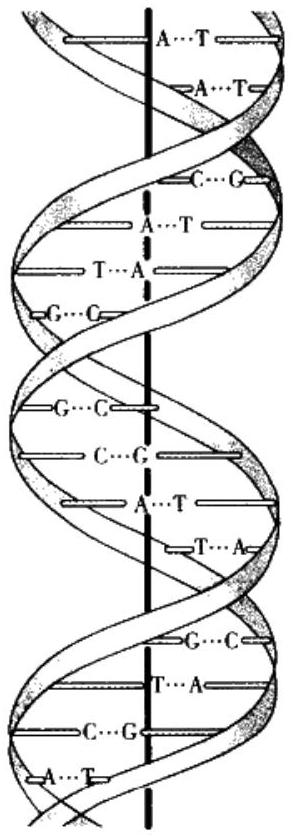
\includegraphics[max width=\textwidth, center]{2025_05_15_6a28331d5e7c993ad07ag-590}

图 13-1 一个互补的双螺旋的示意图。两个糖一磷酸盐的脊椎在外面卷曲着。平躺着的基组成核,它们成对出现——A 总是和 $\mathbf{T}$ 连接, $\mathbf{C}$ 总是和 $\mathbf{G}$ 连接。该结构形成一个螺旋楼梯,成对的基形成胗梯。\\
摘自于 J.D.Watson,The Double Helix.p.130,这里的引用得到版权所有人 G.S.斯坦特的同意。

5 和 6.演绎和检验结果。假说已经形成,接着要对它进行检验。首先,直接的推论是:如果华生和克瑞克提出的双螺旋确实是对 DNA 的正确解释,那么,构造这样一个三维的双螺旋模型是可能的,即所有基都被安排在内部,并且螺旋的角度以及链条的其他特点应当符合以前的 X 光图像及其他的实验结果。这个模型很快就得到了。

许多其他的理论推论被得到,每一个推论的检验都获得了成功。令分子生物学家长期困扰和沮丧的某些数据,由于这样的分析而得以理解。人们了解到,来自于父母的生殖细胞中的 DNA 数量,在普通细胞中只发现了一半。现在我们清楚了个中原因:如果双螺旋在生殖过程中裂开,来自于双亲的裂开的细胞自然只包含正常 DNA 数量的一半。华生一克瑞克对 DNA 结构的解决的正确性的证据迅速增加;不久,他们的假说非常充分

地得到证实。\\
7.应用。华生-克瑞克关于 DNA 结构 128 页的报告 ${ }^{[22]}$ 创造了科学史,它对生物学进程的改变是巨大的也是持久的。该知识的广泛且威力强大的运用将他们的成就推到顶峰。在随后的几十年里,人们认识了 DNA序列中使用的编码;整个人类基因组的完整图实际上是完全的,不久人类将得到该图。将 DNA 链进行切割、重组的技术已经得到发展,它们已经在新药、疫苗和人造荷尔蒙的制造中普遍地得到应用。重新组合 DNA 技术仅在 DNA 结构被最终解决的条件下才是可能的,该技术的应用使生物学和医学发生革命,并且仍保持着旺盛的应用生命力。 
\section{判决性实验和特设性假说}

\begin{quotation}
本节探讨科学方法中的两个重要概念:判决性实验和特设性假说。我们将分析判决性实验如何帮助科学家在竞争性理论之间做出选择,以及特设性假说如何用于保护理论不被反驳证据所否定。通过理解这两个概念,我们将能够更好地评估科学理论的可靠性和科学知识发展过程中的方法论挑战。
\end{quotation}

\subsection{判决性实验}
不同的理论有时会预测相同现象的相同结果;在这种情况下,为了在竞争的理论之间做出选择时,只能使用评判理论的普遍规则。但是当不同的理论对某个现象预测出不同的结果时,科学家便设计出被称做判决性的实验。两个理论中一个所预测的结果是正确的,那么它就通过,如果另外一个所预测的结果是错误的,那么该理论就被拒绝。

科学中的进步很少是直接的和容易的。认为通过对某个问题简单地使用几步假说一演绎法就能够达到答案,这种看法是愚奪的。答案一一正确的说明性假说一一往往是模糊的,需要非常精心制作的理论武器。建立最后的正确假说会极其困难。这个过程完全不是机械的,除了需要艰辛的观察和实验外,还需要深刻的洞察力和很大的创造性。

新的假说得以形成之后,如果它与某个先前已经接受的理论相矛盾,很难确定哪个正确。在某些场合下,两个竞争性假说用被称为一个"判决性实验"的东西进行检验。判决性实验是指这样一个实验,它被精心构造出来以表明所提出的说明中的一个而非另一个实际上是正确的。这样的判决性实验一旦被建立起来,可能是激动人心的和极其有成果的。

例如,美国物理学家阿尔伯特•迈克尔逊和化学家爱德华•莫雷在 1887年精心构造了一个测量光速的实验。通过这个实验使一个被广泛接受的理论(他们原来相信它是正确的)置于一个判决性实验之中。人们长期相信空间中充满着一个被称做"以太"(ether)的假设物质,(人们假定)该物质使光波运行,如同空气使声波运行一样。或者以太存在,或者它不存在。如果它存在,那么测量出的沿着地球运动方向的光速,应当与地球运动成一个直角方向上的光速不同。该实验产生了一个"否定的"结果。因该实验是一个对当时被广泛接受的理论的判决性检验,它成为物理

学史上最著名的实验之一。没有发现这两个不同方向上运动的光速存在差别。这个结果有力地破除了人们长期相信的以太概念。 ${ }^{[23]}$

但是遗憾的是,威力如此强大的判决实验不总是可行的。不同的可观察结果可能不会从不同假说中推演出来;或者,它们能够被推演出来,但是我们没有能力创造条件,以检验哪一个假说的结果将出现。

物理学在 21 世纪初面临的一个主要问题也正属此类。在两个最强有力的理论之间,存在一个明显的目前不能解决的冲突。广义相对论已经得到很好的证实,其定律(描述引力以及引力如何形成空间和时间)的一个必然推论是:某些塌陷的大质量的恒星将形成"黑洞",从该黑洞中逃脱是不可能的,因为它要求比光要快的速度。量子力学定律同样得到很好证实,但它们明确推论得,信息不能永久消失,即使掉到黑洞里也是如此。要么存在某个目前还不知道的时空性质,它能够用来对该信息的保持进行说明,要么在物理学中存在错误,指出它可以对该信息的永久消失给出解释。最终两个理论中的一个必定得到修正,但我们现在仍然不知道哪个要修正,我们也无法构造所需要的判决性实验。 ${ }^{[24]}$

判决性实验是科学探究一个重要方面,然而与构造判决性实验相关的另外一个困难是,人们提出某个说明性假说,我们希望通过进行某个判决性实验来检验它的推论,但它的推论不可能仅从该假说自身演绎出来。我们是使用该假说与其他理论一起而推论得到要检验的结论的。为此,我们假定那些其他理论完全可靠。它们确实可能是完全可靠的,当然它们也可能不完全可靠。如果它们不可靠,即使判决性实验似乎否证了待考察的假说,也有可能待考察的假说恰恰是正确的。科学中的进展依赖于假说集合,其中的任何一个都可能是有缺陷的。

当涉及相当高抽象程度的假说时,仅仅单个假说不可能直接演绎出可直接检验的预测。用做演绎前提的必定是一个统一的假说群体,如果观察到的事实不是预测的事实,那么我们可以得出结论,该假说群中至少一个是错的。但是,这个结论不能表明哪一个假说是错的。例如,在前面的对 DNA 结构发现的解释中,华生和克瑞克在检验核酸丝的形式是双螺旋、它的基指向内部的假说时,他们发现这样的安排不能与所有已知的事实和已接受的理论相一致。"已知的事实和已接受的理论"——水含量、双螺旋斜度、基(腺嘌呤、鸟嘌呤、氧氨嘧啶和胸腺嘧啶)的连接方式——在假说的检验中被假定是正确的。如果所有这些假定的确正确,长丝的结构

不可能是双螺旋。然而,在实际中,华生和克瑞克对他们的假说有足够的自信,他们开始怀疑描述基(A、G、C 和 T )相互结合的理论不完全正确。该理论被他们放弃,他们提出一个不同的理论,即假定结合物是氢的理论,此时,双螺旋的新假说(以及与之相连的理论)得到证实。

因此,在揭示一群假说有缺陷的过程中,一个实验能够是"判决的"。这样一群假说通常包含许多独立的假说。其中任何一个假说,无论实验结果对它多么不利,我们可以拒绝该群体中的某个其他假说,而坚持它的真理性。这就使得某些人得出结论说,从来不会有单个假说遭受判决性的实验。

\subsection{特设性假说}
针对上面的批评,有人认为,一个实验在否证单个新假说中的确能够是判决性的,因为通过拒绝假说群体中某个其他假说(上面已经表明这是可能的)而"拯救"该假说的努力是完全特设的(Ad Hoc)。Ad Hoc 为拉丁术语,字面意义是"为此[特定目的]"。Ad Hoc 包含这样一个意思,所有的假说都是特设的。因为,一个假说之发明如果不是为了解释某个先前得到确立的事实或者其他事实,那是没有意义的。但是当我们以这样的意义滥用它的时候,特设性意味着,对假说集合进行调整仅仅是为了拯救被检验的假说这样一个目的,它没有其他的说明力或者可检验的结果。

没有科学假说是这第二个意义上特设的。如果"鬼是机器故障的原因"被用来解释一个复杂的机器发生故障,那么它明显不是科学的解释;我们嘲笑这样的假说,它是否定意义上特设性的。但是,在任何实际科学研究中,当一个新的假说之提出以调整一个旧的理论的时候,该调整是否是该否定意义上特设性的,这需要进一步确定。

科学史中的另外一个例子可以帮助我们弄清这个问题。在19世纪,天体力学理论被人们很好地理解。对于天文学家来说,天王星和水星这两个行星的轨道与当时所接受的理论对它们所预测的轨道不一致。行星运动的理论在当时应当被修改,但是事实上它被保留了下来。为了解决该理论的协调问题,有人提出,存在某个未发现的行星,其引力造成观察到的反常现象。引起天王星轨道偏差的新行星的轨道,由勒维烈在 1845 年预测出来,预测结果不久被海王星的发现而证实,其位置精确地解释了那些偏 513 差。 ${ }^{[25]}$ 这个假说——存在这样一颗行星——当然不是否定意义上特设性的假说。原因是,从该假说中能够演绎出许多结论,该假说是独立可检

验的。\\
但是在水星的案例中,存在另外一颗行星[该行星过早地被命名为 "火神星"(Vulcan)]干扰水星轨道的假说,不能得到证实。如果一个理论假想有"水星力",用它们来解释水星轨道的异常,而这些力不能解释其他任何事情,并且绝不能被找到,那么这样的一个理论发明自然是特设性的。实际情况是,该疑难长期得不到解决;直到1915年广义相对论提出后,观察到的水星轨道的不规则,才完全与不同的但完美的天文学理论相吻合。水星轨道异常,能够使用广义相对论来预测,这个事实构成该理论最引人注目的证实之一。爱因斯坦称它为"我生命中最辉煌的工作"${ }^{[26]}$ 。只有在那个时候,我们才给出了关于该现象的合适的(即真正理论化的)说明。

天文学史中的这个疑难给出了人们在使用特设性这个术语的第三个意义,它也是否定性的:表示一个单纯的描述性概括。一个描述,它是第三个意义上特设性的,它仅断定一个特定种类的所有事实只在某些特定种类的条件下发生;但是该假说和前面的那些特设假说一样没有任何解释力或解释范围。这样的假说的一个古典例子是,"菲兹吉拉德收缩效应"被提出来对迈克尔逊-莫雷在光速实验结果的解释。菲兹吉拉德断定,物体以极其高的速度运动会发生收缩,他确实对给定现象给出解释,并且他的假说能够为重复进行的同样实验所检验。但是他的"收缩效应"不能解释其他的任何东西。在当时它被普遍认为是特设性的而不是说明性的。(正如与水星行为中出现明显差别的情况一样)直到相对论的提出(爱因斯坦的狭义相对论),人们才得到迈克尔逊一莫雷实验结果的一个合适的理论说明。

我们可这样总结,实验对单个假说绝不能是判决性的,这不仅因为假说经常是在否定意义上特设性的;进一步地说,在本节前面已经表明,因为假说只是在群体中才是可检验的,实验绝不能成为判决单个假说的东西。 ${ }^{[27]}$ 这个限度阐明了科学的系统化特点。科学进步就是建立永远更加恰当(ever-more-adequate)的理论,以便解释不断增加的观察结果和实验事实。某些分离事实能够具有较大的价值,因为科学的最终基础是事实。但是科学结构主要不是通过点滴累积而得以发展的,其发展是在一个已得到普遍认同的理论体系的框架内整体地进行的。认为科学假说或者定律是分散的和独立的观点是朴素的,也是过时的。

在这样一个理论框架中工作,此时我们不对该理论框架进行质疑;进行一个"判决性实验"以证实或否证某个假说的观点仍然能够有意义。如果得到一个否定性结果,即,根据某个有疑问的假说与已经接受的科学理论一道进行预测的某个现象,它没有发生,那么该实验是判决性的,这个有疑问的假说可以被拒绝。但是正如我们已经看到的,在这个过程中不存在任何绝对的事情,因为,那些即使被人们普遍接纳的科学理论面临新的和矛盾的证据时,也要发生调整。科学无论在实践中还是在目标上,都不是一成不变的。

从前面的讨论中得到的启示是,将"隐藏的假设"揭示出来,以便能够对那些默认的假定进行重新审视,这在科学进步中是重要的。当一个关键假设是潜藏的时候,没有明显的必要,因而没有好的机会对之进行考察并确定它到底是真还是假;通过将以前潜藏的假设揭示出来,对之进行分析并(也许)否定它,科学往往获得进步。

例如,在日常生活中谈论两个事件"在同一个时刻"发生,这似乎完全没有问题。我们普遍假定事件常常同时发生。但是科学中一个重要的和巨大的进步开始于爱肉斯坦将这个假定揭露出来。他问,一个观察者如何能够确定两个距离遥远的事件是否真的在同一时刻发生。最终他得出这个结论:两个事件对于某些观察者来说能够是同时的,但对其他的观察者来说则不是;这依赖于观察者相对于待研究事件的相对位置和速度。正是对同时性假定的拒绝,使爱因斯坦发明了狭义相对论,从而为解释迈克尔逊——莫雷实验所揭示的现象跨出了重大的一步。当然,一个假定在它被挑战之前必须被人们所认识,因而,在科学中具有重大意义的是,将理论中起作用的所有有关的假定揭示出来,而不让任何一个隐藏起来。

通过描述和讨论科学史中最辉煌的篇章之一一伽利略对太阳系的哥白尼理论进行的观察证实,是对科学方法的进行总结并阐释科学整体的进步的意义的极好的途径。 

\begin{center}
\fbox{\parbox{0.95\textwidth}{
\textbf{本节要点}
\begin{itemize}
\item \textbf{判决性实验的作用}:
  \begin{itemize}
  \item 在竞争性理论预测相同结果时,依靠普遍评判规则
  \item 当理论预测不同结果时,判决性实验可帮助确定哪个理论更可靠
  \item 真正的判决性实验能够排除某些假说,而保留其他假说
  \end{itemize}
\item \textbf{判决性实验的局限}:
  \begin{itemize}
  \item 科学进步过程复杂,很少有简单直接的决定性实验
  \item 判决性实验不仅要考虑主要假说,还要考虑相关的辅助假说
  \item 批评者认为没有真正单一判决性实验,因为假说总是集群出现
  \end{itemize}
\item \textbf{特设性假说的特点}:
  \begin{itemize}
  \item 特设性假说是为了拯救理论而临时构建的解释
  \item 区别于常规假说的是缺乏独立可检验性和其他说明力
  \item 不能预测新现象,仅用于解释已知的反例
  \end{itemize}
\item \textbf{对特设性假说的评价}:
  \begin{itemize}
  \item 使用特设性假说保护理论违背科学精神
  \item 良好的科学理论应预测尚未观察到的现象
  \item 过度依赖特设性假说的理论往往不是真正科学的
  \end{itemize}
\end{itemize}
}}
\end{center}
\section*{13.7 作为假说的分类}
存在这样一个观点,假说仅在比较发达的科学中而不是在相对不发达的科学中才发挥重要作用。这个观点应当被拒绝。有人主张,尽管说明性假说在物理学、化学这样的科学中起重要作用,它们在生物学和社会科学中则没有这样的作用,或者至少现在没有这样的作用;后者仍然处于描述性阶段,而假说方法对所谓描述性的科学如植物学、历史学是不合适的。我们很容易对这个观点给出反驳。对描述本性的考察将显示,描述本身是建立在假说之上的,或者说描述本身包含假说。假说在生物学的不同体系的分类法或分类学中是基本的,在历史学或其他社会科学中假说也是基本的。

在历史科学中,假说的重要性容易得到阐明,我们首先讨论它。一些历史学家相信,历史研究能够揭示存在着的单个宇宙目的或模式,该目的或模式或者是宗教的或者是自然的,它对有记载的历史的整个进程进行解释或说明。其他的历史学家则否认有任何这样的宇宙设计的存在,但他们坚持认为,历史研究将揭示某个历史规律,该规律解释过去事件的实际次序,并能够用来预测未来。无论哪种观点的历史学家,他们寻求的说明必须解释过去记载的事件,并被它们所证实。因而,无论是哪种观点,历史学是一个理论性的科学而不仅仅是描述性的科学,必须承认假说在历史学家事业中的中心作用。

然而,有第三种历史学家,他们更为谦虚地设定他们的目标。根据他

们的观点,历史学家的任务只是简单地将过去进行编年史记录,即以他们的编年史顺序将过去的事件进行简单的记录。似乎是,根据这种观点, "科学的"历史学家没有进行假说的必要,因为他们所关心的只是事实本身,而非与事实有关的理论。

但是过去的事件没有像该观点试图使我们相信的那样容易编年。过去本身不能提供这种记录。现在能够得到的是现在的记录和过去的痕迹。它们的范围是:从关于过去的官方档案,到对半传说式的英雄的征服行为的赞美的史诗;从以前的历史学家的作品,到考古学家挖掘出土的过去年代的物品。这些只是历史学家能够获得的事实,而从这些事实中他们必须推论得出过去事件的本质——这是他们描述的目的。不是所有的假说是全称的,有些是特称的。历史学家关于过去的描述是特称假说,使用该假说的意图是解释现有数据,而现有数据构成了它的证据。

从大范围来看,历史学家犹如侦探。 ${ }^{[30]}$ 他们的方法是共同的,遇到的困难也类似。其困难主要是证据不充足,并且,许多证据如果不是被笨手笨脚的地方警察所损坏,就是被相关的战争和自然灾害所破坏。正如罪犯可能留下了假的或误导的线索以甩掉追踪者,太多的现存"记录",据说是对过去的描述,而实际上是对过去的歪曲:或者是有意的,如"康斯坦丁的赠款"这样伪造的历史文档的案子,或者是无意的,如早期没有批判性的历史学家的著作。正如侦探建立和检验假说必须使用科学方法一样,历史学家也必须如此。即使将自己限于对过去的纯粹描述的那些历史学家,也必须使用假说来工作:他们是理论家,不管他们自己是如何认为的。

生物学家所处的位置稍微有利。他们处理的事实是现在的,易于检查。为了描述一个地区的动植物群落,他们不必精心构造历史学家那种遭到诟病的复杂推理。数据可以被直接地认识到。对这些项目的描述不是因果的,而只是系统的。他们被认为是对动物和植物进行分类,而不仅仅描述它们。但是分类和描述实际上是同一个过程。将一给定动物描述成食肉类,即是将它分类为一个食肉动物;将它归类为爬行类,即是将它描述成爬行动物。某个物体被描述具有一个给定属性,即是将之归类于具有该属性的对象类中的一个成员。

分类,正如通常理解的那样,不仅仅要将对象划分成不同的群体,而且要将每个群体进一步划分成次一级的群体或次一级的类,等等。这个模

式是我们大多数人所熟悉的:如果不是从学校学习中知道,那么可能是从 "动物,植物,还是矿物?"这个古老的游戏(或者更普遍地被叫做" 20个问题"${ }^{(1)}$ )中获得。分类是一个普遍的需要。原始人不得不将草根、浆果划分为可食用的还是有毒的,将动物分为危险的还是安全的,以及将部落分为友善的还是敌对的。所有人都根据自己的实际需要而进行区分,并忽视那些在他们的事务中不怎么重要的区别。农民会对谷物和蔬莱进行小心和仔细的分类,而将各种花只统称为"花";而卖花人却会细致地将他们的商品进行分类,而将农民的所有收成一起称为"农产品"。

我们对事物进行分类有两个基本的动机。一个是实践的,一个是理论的。某人仅有 3 或 4 本书,他对它们了如指掌,他一瞥就能够分辨它们,就此没有对它们进行分类的必要。但是在一个包含上万册书的图书馆里,情况便不同。如果不对图书进行分类,图书管理员就不能找到所需要的书,该图书馆的收藏将无实际用处。物体数量越大,越有必要对它们进行分类。分类的实际目的是使大量的采集成为可能。在图书馆、展览馆和各类公共记录展厅的情形中这特别明显。

当我们考虑分类的理论用途时,我们必须认识到,使用一种分类法或另一种分类法与真理和错误无关。可以用不同方式、以不同的观点来描述物体。使用的分类方案依赖于分类者的目的和兴趣。例如,图书管理员、图书装订商和藏书家对书的分类便有所不同。图书管理员根据书的内容或主题对书进行分类,图书装订商根据的是装订方式,图书收藏者根据的是印刷日期和相对稀有程度。当然我们不能穷尽各种可能性:图书包装者会根据书的形状和大小对书进行分类,而对书有其他兴趣的人根据他们不同的兴趣进行不同的分类。

那么,科学家的什么样的特别兴趣或目的,使他们偏爱一个分类方案而不是另外一个?科学家的目的是获得知识:不仅仅是关于这个或那个特别的事实的知识,尤其是关于用事实来确认的普遍定律的知识,以及事实之间因果连接的知识。从科学家的观点来看,一个分类方案比另外一个要好,一定程度上在于,在得出科学定律的过程中它是更富于成果的,并且在形成说明性假说过程中它是更有帮助的。

\footnotetext{(1)这是一个游戏。多人确定出一个东西,让另外的人通过询问问题来猜他们所确定的是什么东西。
}对物体进行分类,其理论的或科学的动机是增进这些物体知识的愿望。事物的知识的增加可以增进我们对事物的属性,它们的相似性及差别,以及它们的相互关系的进一步理解。一个分类方案如果只为狭窄的实际目的而制定,就可能抹杀了重要的相似性和差异性。把动物划分成"危险的"和"没有危险的",如把野猪和响尾蛇归为一类,把家猪和草蛇归为一类,这种划分为了强调表面的相似性,而忽视了更本质的相似性。对物体的任何科学的、富有成果的分类需要具有关于它们的大量的知识。对比较明显的特征的粗浅了解,会使人们将蝙蝠作为会飞的生物归为鸟类,把鲸作为生活在大海中的生物归为鱼类。如果我们具有更广阔的知识,我们便将蝙蝠和鲸两者均归为哺乳动物,因为它们都属于温血、胎生并哺育幼崽的动物——这些是分类所根据的更为重要的特征。

如果一个特征能够作为线索,以发现其他特征,它便是重要的特征。从科学的视角来看,一个重要的特征是指这样一个特征:它与许多其他的特征有因果连接关系,因而它能够作为最大数量的因果律的框架,并且有助于形成最普遍的说明性假说。因此,这样的分类方案是最好的,如果它建立在所要分类的物体的最重要的特征之上的话。但是正如我们已经强调的那样,我们事先并不知道会得到哪些因果律,而且因果律本身也带有假设的性质,因而,在哪个分类方案是最好的问题上的决策本身就构成一个假说,一个后续研究可能将之否定的假说。如果后来的研究揭示了,其他特征更为重要(即它与大量的因果律和说明性假说相关),我们能够合理地预期,原来的分类方案应当被否决,我们会选取基于更重要的特征之上的新的分类方案。

分类方式是假说的观点被它在科学中实际所起的作用所证实。分类学是生物学中一个正统的、重要的并且欣欣向荣的分支学科。在生物学中,某些分类方式.如林奈的分类法,被采纳、使用,后来因有了更好的方案而被弃用;更好的方案本身在新的数据下也经受着修改。一般来说,在科学的早期阶段或不发达阶段,分类最为重要。然而,随着科学的发展其重要性不一定总是降低。例如,由门捷列夫表所表明的元素的标准分类法、仍然是化学家的一个重要工具。

前面对自然科学中使用分类的解释,可启发我们进一步认识在历史研究中使用分类的重要性。我们已经说明,历史学家对过去事件的描述本身即是基于冒前资料之上的假说。然而,假说在描述的历史学家的事业中发

挥着另外一个同等重要的作用。任何数量级的历史事件都不能被完完全全地描述。即使人们能够知道它的所有细节,历史学家也不可能将之全部写进著作之中。生命过于短暂,它不允许人们对事物进行详尽无遗的描述。因此,历史学家必须对过去进行有选择地记载,记录下的仅仅是过去的一些特征。历史学家进行选择的基础是什么?显然,历史学家要叙述的是有意义的或重要的,而忽略无意义的或琐碎的。这个或那个历史学家的主观偏见会使他或她过分强调历史进程中宗教、经济、人物或其他某个方面的作用。但如果历史学家们考虑到,要做出客观的或科学的评价,他们便会重视那些能够形成因果律和普遍的说明性假说的因素。自然,这样的评价会随着进一步研究而经受着改变。

西方第一个历史学家希罗多德(Herodotus)细致描写了他编入编年史的事件,有人物的、文化的,以及政治的、军事的。所谓第一位科学的历史学家修昔底德,将自己的写作更多地限于政治和军事方面。在很长一段时间里,大多数历史学家跟随修昔底德,但是现在钟摆正摆向另外一个方向:历史学家十分重视过去的经济和文化方面。正如生物学家的分类方案包含了他们的假说——通过这个假说生物的特征与最大数量的因果律相关联,历史学家选择用一个典型事件集合而非另外一个集合来描述过去事件,这种选择包含了他们的假说:什么样的典型事件与最大数量的其他典型事件因果地连接在一起。这样的假说是必需的,哪怕历史学家对过去进行系统的描述的工作只是刚刚开始。正是分类和描述——无论是生物学的还是历史学的一一所具有的假说性的特点,使我们将假说看成是科学探究的通用方法(the all-method)。 

% 第十四章
\section{第14章 概率与归纳逻辑}

\begin{quotation}
\textit{概率是归纳逻辑的核心工具,通过它我们能够量化不确定性,评估科学假说的可靠性,并在日常生活中做出更加明智的决策。本章探讨概率的不同解释及其在推理中的应用。}
\end{quotation}

\section{关于概率的几种观点}

\begin{quotation}
\textit{概率有多种解释,每种解释都映射了我们理解不确定性的不同方式,掌握这些视角能够帮助我们更全面地理解归纳推理。}
\end{quotation}

在归纳逻辑中,\textbf{概率}(probability)是一个核心概念,在前面关于科学方法的讨论中已多次阐述。一个假说即使符合所有接触到的事实,它也不是决定性地得以确立;它只具有或然性。我们看到,即使我们慎之又慎地使用实验探究的密尔方法,也不能决定性地证明我们所得到的因果律的真理性,而只是以高的或然性(概率)确证它们。即使最好的归纳论证也不具有有效演绎论证所拥有的那种确定性。

因而,恰当地说,我们对归纳逻辑的考察离不开对概率这个关键概念的分析。我们必须区分"盖然的"(probable)和"概率"的不同用法。下面三个命题显示了概率的最典型的用法:

1.一个投出去的硬币出现正面的概率是 $1 / 2$ 。

2.一个 25 岁的妇女过 26 岁生日的概率为 0.971 。

3.基于现有的证据,爱因斯坦相对论的正确性是高度盖然的。

存在使用"盖然的"和"概率"的其他情境,如我们说测量中的"可能错误"(probable errors),但这三种是最重要的。在前两个命题中,一个数字——被称为概率数值——被赋予一个特定事件;第三个命题则不同,它没有被赋予这样的数字。当我们谈论一个可疑的科学假说时,我们通常赋予一个盖然程度。比如,人们说达尔文理论比《创世记》中对生命起源的解释更可靠(probable),再比如,原子理论具有比其他的关于原子核内部结构的假说有较高的盖然度。

前两个例子中所给予的数字是十分有用的,并且似乎十分合理。但它们从何处得来?

硬币有两面:正面和反面。当硬币落地时,必定有一面朝上。两个机会中的一个机会是正面向上,因此以概率 $1 / 2$ 赋予正面。为了得到第二个例子中的概率值,我们必须进行死亡率统计并进行比较。在 1000 个庆祝

正如前两个例子所表明的,概率研究与赌博和死亡统计有关;事实上,现代概率研究开始于这两个领域。熟知的是,概率论起步于帕斯卡 (Blaise Pascal,1623-1662)和费玛(Pierre Fermat,1608-1665)关于机会赌博中合理赌注的通信,另外一种说法是,概率起源于帕斯卡给切瓦里•德•梅尔(Chevalier De Mere)一一个著名的赌徒——如何在掷骰子时下赌注的建议。与死亡率相关的是,自从1592年伦敦开始保存死亡记录;1662年,约翰•格朗特上尉发表了对这些记录的一个研究,探讨了从这些记录中用概率能够推得什么。可能是因为这复合的血缘,概率有如下两种解释。

\subsection{概率的先验解释}

经过拉普拉斯、德摩根、凯恩斯等人的发展,关于概率本质的古典理论认为,概率是合理信念(rational belief)度的测定。当我们完全相信某个事情,我们信念度的测定被赋予数字1。当我们绝对相信一个特定事件不可能发生,该事件将发生的信念度被赋予数字 0 。因而,一个理性人在一个掷出去的硬市或者出现正面或者不出现正面上的信念度是 1 ;既出现正面又不出现正面的信念度是 0 。当他不能肯定的时候,他的合理信念度将为 0 和 1 之间的某个数。概率是关于事件的一个属性,它是人们合理地相信一个事件将发生的程度。或者说,概率是一个陈述或命题的谓词,一个完全理性的人总是依据这个值相信该陈述或命题。

在古典理论看来,概率总是部分有知和部分无知的结果。如果我们能够知道掷硬市的手指的精确运动,加上硬币的初始位置、大小、重量分布,人们确信能够预测硬市的轨道以及最后的不动的位置。但是,这些完全的信息不可能得到。我们只能知道某些信息:硬币有两面;它将下落;等等。因此,硬币正面向上的信念度由几种可能性所决定——这里可能性为 2 个、出现正面的可能性为 1 个。因而, $1 / 2$ 的概率值被赋予硬市出现正面的事件。类似的,人们要分发一副纸牌时,纸牌以一确定的顺序被分发。如果发牌诚实,牌中的黑桃、红桃、方块、梅花,以及 A、K、Q、 $J$ ,均以洗牌时确定的次序而得以分发。但我们不知道这个次序。我们只知道总共的 52 张牌中有 13 张黑桃,因此,所发的第一张牌为黑桃的概率精确地为 $13 / 52$ ,或者 $1 / 4$ 。

这些观点为概率论的先验论观点。之所以如此称呼,是因为无须做实验,也无须选择样本来考察,就可以得到概率。只需要知道先行条件:纸牌中只有 13 张黑桃;总共有 52 张牌;发牌是诚实的,任何一张牌与其他牌有同样的机会被第一次分发。以先验的观点,为了计算在某些特定情形下一个事件发生的概率,我们把该事件能够发生的途径数,除以该情形下可能的结果总数——如果我们没有任何理由相信任何一个可能的结果比其他的更有可能的话。于是,一个事件的概率以一个分数来表示,其中,除数是等可能的结果总数,被除数是使待考察事件发生的结果数。一种诚实地出售 1000 张彩票的彩票发行,有 1000 个等可能的结果。因而,其中任何一张彩票能够中彩的概率是 1 除以 1000 ,即 $1 / 1000$ 。

\subsection{概率的相对频率解释}

与先验论不同的一个理论认为概率是相对频率的一个度量。相对频率理论特别适合解释统计研究的概率判断。例如,保险公司精算师希望确定 25 岁妇女的死亡率。这里,我们有一个对象总体和一个属性:这个总体是 25 岁的妇女;属性是活到 26 岁生日。该理论中,赋予的概率是这样的相对频率测度:该人群以这个频率体现了这个被研究的属性。这里同样的是,概率也表示成分数。不过,在这里,分母是对象总体数量,分子是具有该属性的对象的数量。如果考察了 1000 个 25 岁的妇女的记录,发现其中有 971 个活到 26 岁生日,那么 0.971 就是该对象总体出现该属性的概率系数。这里没有出现合理信念。在概率的相对频率理论中,概率被定义成总体成员体现某一特定属性的相对频率。

必须说明的是,在这两个理论中,被赋予的概率是相对于采集的证据而言的。在相对频率理论中这是明显的。因为一个给定属性的概率,必定随着选择用来计算的特定对象总体的变化而变化。在上面用到的例子中,构成研究总体的 1000 名妇女是随机地从埃及人中选取,人们会发现,活到 26 岁的这个频率,将与随机地从法国人中选取的 1000 名妇女活到 26岁的概率不同。 25 岁的妇女再活 1 年的概率在埃及和在法国是不同的。类似的,在斯堪的纳维亚地区的人口总体中金发的概率高于在世界总人口中金发的概率。因此,在使用概率的相对频率理论时,一个关键的步骤是选择最合适的研究总体。

但是,在先验理论那里概率也是相对的。根据该理论的古典解释,任何事件均不具有内在的概率。一个事件的概率值之获得只能建立在做出其概率值指派的人所获得证据之上。这样的概率被解释成这样的一个观点,概率为合理信念的测度,因为一个理性人的信念随着他的知识的变化而变化。

譬如,假设两个人观看洗牌。当洗牌完成时,洗牌者因某个偶然的因素意外地使最上面的一张牌"露"了一下。第一个观察者看到了那张牌是黑的,但他没有看到是黑桃还是梅花。第二个观察者没有任何察觉。如果让这两个观察者估计第一张牌是黑桃的概率,第一个观察者将指派概率值 $1 / 2$ ,因为他知道有 26 张牌(黑色的牌),其中一半是黑桃。但第二个观察者将指派概率值 $1 / 4$ ,因为他知道的仅仅是 52 张牌中黑桃为 13 张。两个观察者对同一个事件指派了不同的概率。其中一个观察者犯了错误?当然没有:每个人相对于可用证据赋予了正确的概率。即使这张牌被翻开后为梅花,两个人的估计均是正确的。任何事件自身不具有内在的或关于它的概率。这里的意思是,任何预测所具有的不同概率是相对于不同背景而言的,即相对于不同证据集而言的。然而,人们在做出概率断定之前,应当尽可能地寻求收集最大量的证据集。

\subsection{概率解释的对比与融合}

概率的这两种解释——相对频率解释和先验解释——在认为概率是相对于证据的这一点上是一致的。因而,这两个理论的信奉者在接受和使用概率计算上也是一致的。下一节将介绍概率计算的初步知识。

\begin{center}
\fbox{\parbox{0.95\textwidth}{
\textbf{本节要点}
\begin{itemize}
\item \textbf{概率在归纳逻辑中的重要性}:
  \begin{itemize}
  \item 概率是归纳推理的核心概念
  \item 科学假说只能达到或然性而非确定性
  \item 概率为不确定性提供量化手段
  \end{itemize}
\item \textbf{概率的先验解释}:
  \begin{itemize}
  \item 概率被视为合理信念的测度
  \item 通过可能结果的数学比例计算
  \item 无需实验即可推导,如$P(硬币正面)=1/2$
  \end{itemize}
\item \textbf{概率的相对频率解释}:
  \begin{itemize}
  \item 概率表示属性在总体中出现的频率
  \item 基于观察数据和统计分析
  \item 适用于经验研究,如保险精算
  \end{itemize}
\item \textbf{两种解释的共同点}:
  \begin{itemize}
  \item 概率都是相对于证据而言的
  \item 概率值会随可用证据的变化而变化
  \item 两种方法在概率计算上可以兼容
  \end{itemize}
\end{itemize}
}}
\end{center} 
\
\\section*{14.2 概率计算}
我们来确定一个复合事件的概率。复合事件可以被看做由多个事件构成的整体。例如,我们问:从一副牌中连续抽出两张黑桃的概率是多少?连续抽两张牌这样的复合事件是一个由两个部分组成的整体。这两个部分是,第一次抽出黑桃的事件,和第二次抽出黑桃的事件。再举一个例子,新娘和新郎活到庆祝金婚纪念日的复合事件,是由新娘再活 50 年的事件和新郎再活 50 年的事件,以及不发生离婚的事件组成的。当人们知道各个组成事件是如何相互关联的时候,人们能够根据单个事件的概率而求得该复合事件的概率。因而,我们把"概率计算"——用单元事件的概率计算出复合事件的概率——规定为纯数学的一个分支。

概率计算在日常生活中是极其有用的。知道某个结果的可能性可以帮助我们进行决策,而使我们做事谨慎。因而,其基本定理的掌握和运用是逻辑研究最有用的结果之一。

概率计算最容易用机会游戏(games of chance)——掷骰子、玩扑克等等——的术语来解释。原因是,这些游戏所限定的人工世界使概率定理的直接使用成为可能。因此,尽管概率计算有广泛的应用范围,在这一章中,我们通过赌博中引申出来的问题,初步地阐明概率计算。在阐释过程中我们使用了概率的先验理论,当然,所有结果经过少量的重新解释后也能够用相对频率理论来表述和分析。 
\section{共同发生的概率}

\begin{quotation}
\textit{当我们需要计算多个事件同时发生的可能性时,理解事件之间的独立性关系至关重要。通过掌握乘法定理,我们能够解决从赌博到医疗决策的各种复杂概率问题。}
\end{quotation}

\textbf{共同发生}(joint occurrences)是指某个复合事件的单元事件中的两个或两个以上事件的发生。我们希望知道从一副牌中连续抽出 3 张黑桃的概率,或者在一场赛马中喜爱的两匹马都使我输钱的概率,或者将一枚硬币扔十次得到十次正面向上的概率。假定我们正考察的是只有两个单元事件 $a$ 和 $b$ 的发生。当我们要得到 $a$ 并且 $b$ 两者的概率时,我们便要求它们的共同发生。

\subsection{独立与非独立事件}

一个困难立即出现了:两个事件中的一个出现或不出现对另外一个事件的出现或不出现产生影响吗?如果存在这样的影响,单元事件就不独立;如果不存在这样的影响,它们就是独立的。如果两个事件中的一个的发生或不发生对另外一个事件的发生或不发生,不产生任何影响,我们说两个事件是\textbf{独立的}。例如,如果我们掷两枚硬币,无论一枚硬币是正面朝上还是反面朝上,不会影响另外一枚硬币是正面朝上还是反面朝上;它们是独立的事件。

\subsection{独立事件的共同发生}

为了讨论事件共同发生的概率,我们先分析比较容易的情况:独立事件的共同发生。考虑这样一个简单问题:掷两枚硬币,两枚均正面朝上的概率是多少?掷两枚硬币有三个可能结果:或两个正面,或两个反面,或一正一反。但是它们不是等可能的。因为,有两种方式发生一正一反,而只有一种方式得到两个正面。第一枚硬币出现正面,第二枚硬币出现反面;或者第一枚硬币出现反面,第二枚硬币出现正面,它们是不同的情况。因而,当我们掷出两枚硬币时,可能出现 4 个不同的可能事件。将之列表如下:

\begin{center}
\begin{tabular}{|c|c|}
\hline
\textbf{第一枚硬币} & \textbf{第二枚硬币} \\
\hline
正 & 正 \\
正 & 反 \\
反 & 正 \\
反 & 反 \\
\hline
\end{tabular}
\end{center}

没有理由期望其中的任何一个情况比其他情况更可能发生,因而我们认为它们是等可能的。两枚正面朝上的特别情形只是 4 个等可能的事件之一,因此,掷出两枚硬币,得到两次正面的概率是 $1 / 4$ 。这个复合事件的概率可以通过两个独立的单元事件的概率而求得。该复合事件由第一次掷出正面和第二次掷出正面,这两个事件的共同发生所构成。第一次掷出正面的概率为 $1 / 2$ ,第二次掷出正面的概率也为 $1 / 2$ 。这两个事件是独立的,因而我们可以用概率计算的\textbf{乘法定理}来计算它们共同发生的概率。根据独立事件的乘法定理,两个独立事件共同发生的概率等于它们各自概率的乘积。这个一般公式可以写成:

$$
P(a \text { 且 } b)=P(a) \times P(b)
$$

这里,$a \zhtext{、} b$ 为两个独立事件,$P(a)$ 和 $P(b)$ 为它们的概率,而 $P(a$ 且 $b)$为 $a \zhtext{、} b$ 共同发生的概率。本例中,$a$ 为第一次出现正面的事件,$b$ 为第二次得到正面的事件,这样,$P(a)=1 / 2, P(b)=1 / 2$ ;因此,$P(a$ 且 $b)=$ $1 / 2 \times 1 / 2=1 / 4$ 。

\subsection{骰子问题的概率}

考虑第二个问题。我们摇两个骰子,得到 12 点的概率为多少?只有当每个骰子都为 6 点,两个骰子才出现 12 点。每个骰子有 6 面,摇后每一面向上与其他面向上的可能性相同。假定 $a$ 为第一个骰子出现 6 点的事件,$P(a)=1 / 6$ ;假定 $b$ 为第二个骰子出现 6 点的事件,$P(b)=1 / 6$ 。 $a$ 和 $b$ 的共同发生构成了两个骰子出现 12 点的复合事件。根据乘法定理, $\mathrm{P}(\mathrm{a}$ 且 b$)=1 / 6 \times 1 / 6=1 / 36$ 。 $1 / 36$ 即为要两个骰子得到 12 点的概率。我们也可以通过列举摇两个骰子时所有可能发生的事件,而求得同样的结果。有 36 个等可能事件,列表如下。在表中,每一对数字中的第一个数字代表第一个骰子向上的数字,第二个数字代表第二个骰子向上的数字。

\begin{center}
\begin{tabular}{|c|c|c|c|c|c|}
\hline
1-1 & 2-1 & 3-1 & 4-1 & 5-1 & 6-1 \\
\hline
1-2 & 2-2 & 3-2 & 4-2 & 5-2 & 6-2 \\
\hline
1-3 & 2-3 & 3-3 & 4-3 & 5-3 & 6-3 \\
\hline
1-4 & 2-4 & 3-4 & 4-4 & 5-4 & 6-4 \\
\hline
1-5 & 2-5 & 3-5 & 4-5 & 5-5 & 6-5 \\
\hline
1-6 & 2-6 & 3-6 & 4-6 & 5-6 & 6-6 \\
\hline
\end{tabular}
\end{center}

在 36 个等可能的情况中,只有 1 个为我们希望的(出现 12 点),因而,我们直接得到概率为 $1 / 36$ 。

\subsection{乘法定理的推广}

我们可以将乘法定理一般化,以便涵盖任意多个独立事件的共同发生。如果我们从一副牌中抽出一张牌,将之放回并抽第二次牌,再放回去并抽第三次牌,那么抽出三次黑桃的事件,为第一次抽出黑桃的事件、第二次抽出黑桃的事件和第三次抽出黑桃的事件共同发生所构成。这三个事件用 $a \zhtext{、} b \zhtext{、} c$ 来表示,它们共同发生的概率 $P(a$ 且 $b$ 且 $c)$ 等于三个事件各自概率的乘积:$P(a) \times P(b) \times P(c)$ 。这个概率容易计算出来。一副扑克有 52 张牌,其中 13 张为黑桃。因此,抽出一张黑桃的概率为 $13 / 52=1 / 4$ 。由于再次抽牌之前原先抽出的牌被放了回去,第二次抽牌的情况与第一次的一样,因而,$P(a) \zhtext{、} P(b) \zhtext{、} P(c)$ 均为 $1 / 4$ 。它们共同发生的概率为 $P(a$ 且 $b$ 且 $c)=1 / 4 \times 1 / 4 \times 1 / 4=1 / 64$ 。我们可以用通用乘法定理计算任意多个独立事件共同发生的概率。

\subsection{非独立事件的共同发生}

现在我们转向分析不独立的事件。将独立事件的概率简单相乘,如上面的例子中所做的,没有考虑单元事件之间的关系。如果那些事件是有关联的,我们需要将这种关系考虑进来,以便精确计算这样的事件的共同发生。我们经常能够这样做。将上述例子做些修改。假定我要求从一副洗好的扑克牌中连续抽三张黑桃的概率,但抽出的牌不放回去。如果每一次抽出的牌在下次抽牌之前不放回去,前面的抽牌结果确实对后面的抽牌结果产生影响。如果抽出的第一张牌是一张黑桃,那么第二次抽牌过程中总的牌数为 51 张牌,剩下的黑桃有 12 张。而如果第一次抽出的不是一张黑桃,那么,剩下的 51 张牌中有 13 张黑桃。假定 $a$ 是从一副牌中抽出一张黑桃并且不放回去的事件,$b$ 为从剩下的牌中抽取另外一张黑桃的事件,那么 $b$ 的概率,即 $P($在 $a$ 发生的条件下 $b)$[我们用 $P(b \mid a)$ 来表示 $P(a$条件下 $b$ )一一译者]为 $12 / 51$ ,即 $4 / 17$ 。如果 $a$ 和 $b$ 都发生,第三次抽牌是在只有 11 张黑桃的 50 张牌中进行。如果 $c$ 是最后的事件,那么\\$P(c \mid a$ 且 $b)$[即 $P($ 在 $a \zhtext{、} b$ 发生的条件下 $c)$ ]为 $11 / 50$ 。于是,从一副牌中抽取三张牌、抽完不放回去,根据乘法定理,三张均是黑桃的概率为 $13 / 52 \times 12 / 51 \times 11 / 50$ ,即 $11 / 850$ 。这个值小于抽三张牌、但每次抽牌后放回去的概率。这也是我们能够预知的,原因是将抽出的牌放回去增加下次抽到黑桃的概率。

\subsection{条件概率与通用乘法定理}

我们来看另外与不独立事件共同发生的概率有关的一个例子。假定有一个袋子,袋子里面有 2 个白球和 1 个黑球。如果我们连续摸两个球,并且第一次摸到的球在第二次摸球之前不放回去,两次摸到的均是白球的概率是多少?假定 $a$ 为第一次摸到白球的事件。有三个等可能性,每个可能性对应于其中一个球。由于两个球为白色的,其中两个可能性能得到白球。因而,第一次摸到白球的概率为 $2 / 3$ 。如果 $a$ 事件发生了,袋中只剩下了两个球,一白一黑。明显的,第二次摸到白球(我们用 $b$ 表示)的概率为 $1 / 2$ ,即 $p(b \mid a)=1 / 2$ 。据通用的乘法定理,摸到两次白球的概率为 $a$ 和 $a$ 条件下 $b$ 共同发生的概率,其值为它们各自发生的概率值的乘积, $2 / 3 \times 1 / 2=1 / 3$ 。通用公式为:

$$
P(a \text { 且 } b)=P(a) \times P(b \mid a)
$$

在这个简单的情况下,我们可以通过计算各个可能的情形而确定连续两次摸到两个白球的概率。我们用 $W_{1}$ 表示一个白球,$W_{2}$ 表示另外一个白球,$B$ 表示黑球,下表列举了所有可能的等可能情况:

\begin{center}
\begin{tabular}{|c|c|}
\hline
\textbf{第一次摸球} & \textbf{第二次摸球} \\
\hline
$W_{1}$ & $W_{2}$ \\
$W_{1}$ & $B$ \\
$W_{2}$ & $W_{1}$ \\
$W_{2}$ & $B$ \\
$B$ & $W_{1}$ \\
$B$ & $W_{2}$ \\
\hline
\end{tabular}
\end{center}

在这 6 个等可能的事件中,两种情形是我们需要的(第一和第三)。连续两次摸球、第一次摸到的球不放回去的概率,我们可以直接求得为 $1 / 3$ 。

\subsection{现实应用:医疗决策中的概率}

通用乘法定理可以用于对现实世界问题的后果估计,下面就是一个例子。一个加利福尼亚少女受慢性白血病的折磨。如果不治疗,它将因白血病而死去。只有找到匹配的骨髓捐赠者,她才能得救。当她的父母寻找这样的捐赠人的所有努力均失败之后,他们决定再生一个小孩,以希望能够成功进行骨髓移植。但她的父亲首先得将切断的输精管接通,这只有 $50\%$ 的成功率。如果成功了,她的母亲因当时有 45 岁,她怀孕的机会也只有 $0.73$ 。如果她确实受孕成功,婴儿骨髓与受病痛折磨的女儿匹配的机会也只有四分之一( $0.25$ )。并且即使匹配成功,白血病病人经过必需的化疗和骨髓移植后活下来的机会为 $0.70$ 。

可以看到的是,结果成功的概率很低,但不是低到毫无希望。输精管成功得到接通,母亲也确实怀孕了,至此,希望增加了。巧的是,婴儿拥有能够匹配的骨髓。1992年进行了艰巨的骨髓移植手术。手术获得巨大成功。 ${ }^{[1]}$ 这个美满结果其概率在她的父母做决策的时候有多大呢?

\section*{乘法定理}
为了计算两个或更多事件共同发生的概率:

\begin{center}
\begin{tabular}{|p{0.95\textwidth}|}
\hline
\textbf{A.如果这些事件(如 $a \zhtext{、} b$ )是独立的:} \\
它们共同发生的概率为其概率的简单乘积:
$P(a \text { 且 } b)=P(a) \times P(b)$ \\
\hline
\textbf{B.如果这些事件(如 $a \zhtext{、} b \zhtext{、} c$ 等)是不独立的:} \\
它们共同发生的概率为第一个事件的概率乘以第一个事件发生的条件下第二个事件的概率,乘以第一和第二个事件发生的条件下第三个事件的概率,等等。 \\
$P(a \text{ 且 } b \text{ 且 } c)=P(a) \times P(b \mid a) \times P(c \mid a \text{ 且 } b)$ \\
\hline
\end{tabular}
\end{center}

\begin{center}
\fbox{\parbox{0.95\textwidth}{
\textbf{本节要点}
\begin{itemize}
\item \textbf{共同发生的基本概念}:
  \begin{itemize}
  \item 共同发生指多个事件同时发生的复合事件
  \item 事件的独立性决定了计算方法的不同
  \item 共同发生的概率总小于单个事件的概率
  \end{itemize}
\item \textbf{独立事件的共同发生}:
  \begin{itemize}
  \item 独立事件指一个事件发生与否不影响其他事件
  \item 概率通过简单乘法计算:$P(a \text{ 且 } b) = P(a) \times P(b)$
  \item 适用于硬币投掷\zhtext{、}骰子摇动等相互无关的情形
  \end{itemize}
\item \textbf{非独立事件的共同发生}:
  \begin{itemize}
  \item 一个事件的发生会改变其他事件的概率
  \item 通用乘法定理:$P(a \text{ 且 } b) = P(a) \times P(b|a)$
  \item 常见于抽牌不放回\zhtext{、}连续选取等情境
  \end{itemize}
\item \textbf{条件概率的应用}:
  \begin{itemize}
  \item 条件概率表示为$P(b|a)$,指在事件a发生条件下b的概率
  \item 通用乘法定理可扩展到任意多个事件
  \item 在现实应用中帮助评估复杂事件的可能性
  \end{itemize}
\end{itemize}
}}
\end{center}

% The rest of the file, including exercises, is removed. 
\section*{14. 4 替代性发生的概率}
我们有时对一系列事件中的一个或多个发生的概率感兴趣。例如,当我们掷两枚硬币时,我们想知道一枚或另外一枚着地时正面向上的可能性是多少。在抽两张牌的扑克牌游戏中,我们想知道抽到或者一张黑桃或者一张梅花的概率为多少。替代性发生的概率 ${ }^{(1)}$ 总是大于每个事件发生的概率。如同在共同发生的情况下,两个事件共同发生的概率将小于其中一个单独事件发生的概率。

人们如何计算替代性发生的概率?在共同发生的情况下我们将两个分数相乘,得到了一个低的概率值。不同的是,当我们求替代性发生的概率时,我们将分数相加,概率值增加。然而,我们同样碰到了复杂的情况,需要我们将之分为两类进行考虑。

替代性发生的事件可能是相互排斥的,也可能不是相互排斥的。两个事件如果不能同时发生,它们便是相互排斥的。如果我掷两枚硬币并得到两个正面,我不能在这两次投掷中得到两次反面。两个正面和两个反

\footnote{(1)这里将 alternative occurrence 译成"替代性发生",意为两个或两个以上的事件至少一个发生,亦可译为"择代性发生"。}面明显是相互排斥的。但是如果我从一副牌中抽取两张牌,两张牌中一张是黑桃或一张是梅花,是可以出现的不同情形。在一副牌中抽取两张牌,"抽到一张黑桃"和"抽到一张梅花"不是相互排斥的事件。计算替代性发生概率的方法将因事件是否为相互排斥而大大不同。我们依次来分析。

如果事件是相互排斥的,计算直接而且容易:将两个事件的概率进行简单相加即可。将一枚硬币掷两次,出现两次正面或者两次反面的概率是多少?自然的是,一个概率与另外一个概率相加。两次正面的概率为 $1 /$ 4 ,两次反面的概率为 $1 / 4$ ,或者两次正面或者两次反面的概率为 $1 / 4+1 /$ $4=1 / 2$ 。

计算两个相互排斥事件构成的复合事件的概率公式为:

$$
P(a \\text { 或 } b)=P(a)+P(b)
$$

这是加法定理,它可以推广到适合任意多的事件( $a, b, c \\cdots \\cdots$ )。如果所有的事件是相互排斥的,它们中至少一个发生的概率为它们的概率和。

通过对扑克牌游戏中能够被分发到同花色牌(5 张牌为同一种花色)的概率的计算,我们来说明上面的公式。这里,有四个相互排斥的可能性:拿到 5 张黑桃的事件,拿到 5 张红桃的事件,拿到 5 张梅花的事件,拿到 5 张方块的事件。让我们先来计算拿到 5 张黑桃的概率。这是一个由 5 个明显非独立的子事件构成,因为分发到黑桃将减低下面得到黑桃的概率。利用非独立的乘法定理,我们有 $13 / 52 \\times 12 / 51 \\times 11 / 50 \\times 10 / 49 \\times$ $9 / 48=33 / 66640$ 。其他每一个可能性(5 张红桃、5 张梅花、5 张方块)均有与此相同的概率。这 4 种同花色是相互排斥的事件,因此,利用加法定理,得到任何一种同花色的概率为 $33 / 66640+33 / 66640+33 / 66640+$ $33 / 66640=33 / 16660$ 。

再举一个例子。从两个袋子中各摸一个球,一个袋子中有两个白球和 4 个黑球,另一个袋子中有 3 个白球和 9 个黑球,摸到两个同颜色的球的概率是多少?我们感兴趣的概率的事件是两个互斥事件的替代性发生:一个是摸到两个白球的事件,另外一个是摸到两个黑球的事件。分别计算这两个事件的概率,然后相加。摸到两个白球的概率为 $2 / 6 \\times 3 / 12=1 / 12$ ;摸到两个黑球的概率为 $4 / 6 \\times 9 / 12=1 / 2$ 。因此摸到两个同样颜色的概率

为 $1 / 12+1 / 2=7 / 12$ 。\\\\到目前为止,我们对替代性发生的讨论都是针对互斥事件。但是我们必须计算由非互斥的两个或更多的事件中至少一个发生的复合事件的概率。例如,将一枚硬币掷两次,至少得到一次正面的概率是多少?事件不是互斥的,因为可以肯定的是,能够两次投掷都得到正面。我们清楚,第一次投掷得到正面的概率为 $1 / 2$ ,第二次投掷得到正面的概率也是 $1 / 2$ ,但这两个概率之和为 1 ,即事件为确定的,然而至少一次投掷为正面是不确定的!这个例子说明,当我们计算非互斥事件替代性发生的概率时,加法定理不能直接应用。我们可以用两个间接的方法来计算这种类型的概率。

计算两个非互斥事件中至少一个发生的概率的第一个方法,要求我们将事件分解成互斥事件。在求解将一枚硬市投掷两次得到至少一面为正面的概率的问题中,等可能的状态是 $\\mathrm{H}-\\mathrm{H}, \\mathrm{H}-\\mathrm{T}, \\mathrm{T}-\\mathrm{H}, \\mathrm{T}-\\mathrm{T}$ 。它们是相互排斥的,每一个状态的概率为 $1 / 4$ 。前三个状态为我们要求的;即在前三个状态中的任何一个状态发生的条件下,两次投掷中至少一次为正面就是真的事实。于是,投掷出至少一面为正面的概率,等于所有符合要求的互斥状态的单独概率之和,即为 $1 / 4+1 / 4+1 / 4=3 / 4$ 。

计算两个非互斥事件中至少一个发生的概率的另外一种方法,建立在这样的事实上,没有状态既是满足条件的又是不满足条件的。我们用 $a$ 表示将一枚硬币投郑两次得到至少一次正面的事件,那么,我们用符号 $\\bar{a}$ 表示与 $a$ 不同的事件,即两次投掷没有一次正面的事件。因为没有状态既是我们需要的又是我们不需要的,$a$ 与 $\\bar{a}$ 是相互排斥的,$a$ 与 $\\bar{a}$ 不能都发生。由于每个状态必定是,或者是这个事件或者不是这个事件,可以肯定的是,或者 $a$ 或者 $\\bar{a}$ 必定发生。我们给不能发生的事件指派概率值 0 ,给必定发生的事件指派概率值 1。下面两个等式是成立的:

$$
\begin{aligned}
& P(a \\text { 且 } \\bar{a})=0 \\\\
& P(a \\text { 或 } \\bar{a})=1
\end{aligned}
$$

这里,$P(a$ 且 $\\bar{a})$ 为 $a$ 和 $\\bar{a}$ 均发生的概率,$P(a$ 或 $\\bar{a})$ 为 $a$ 或者 $\\bar{a}$ 发生的概率。由于 $a$ 和 $\\bar{a}$ 是互斥的,可以应用加法定理。我们得到:

$$
P(a \\text { 或 } \\bar{a})=P(a)+P(\\bar{a})
$$

$$
P(a)+P(\\bar{a})=1
$$

由上式得到非常有用的等式:

$$
P(a)=1-P(\\bar{a})
$$

于是,我们可以通过计算一个事件不发生的概率,再用 1 减去这个数,就得到一个事件发生的概率。我们应用这个方法来求投掷两次硬币得到至少一次正面事件的概率。我们容易看到,该事件不发生的唯一情况为,两次投郑均为反面——这是不满足条件的状态,由乘法定理,概率值为 $1 / 2 \\times$ $1 / 2=1 / 4$ ,据此,投郑两次硬市中得到至少一次正面事件确实发生的概率为 $1-1 / 4=3 / 4$ 。

一个事件由多个可能的但不相互排斥的事件的替代性发生,所组成的另外一个例子如下。从两个袋子中各摸一个球,其中:第一个袋子里有 2个白球和 4 个黑球,第二个袋子有 3 个白球和 9 个黑球。至少摸到一个白球的概率为多少?上面两个方法中的任何一个都可以用来求解这个问题。我们将满足条件的状态分为互斥的状态。它们是,从第一个袋子里摸到一个白球和从第二个袋子里摸到一个黑球;从第一个袋子里摸到一个黑球和从第二个袋子里摸到一个白球;以及从两个袋子里均摸到白球。这三个事件的概率分别为: $2 / 6 \\times 9 / 12=1 / 4,4 / 6 \\times 3 / 12=1 / 6$ ,及 $2 / 6 \\times 3 /$ $12=1 / 12$ 。据互斥事件的加法定理,至少摸到一个白球的概率为 $1 / 4+$ $1 / 6+1 / 12=1 / 2$ 。另外一个方法稍微简单些。不满足条件的状态——没有摸到至少一个白球的事件——为摸到两个黑球的事件。摸到两个黑球的概率为 $4 / 6 \\times 9 / 12=1 / 2$ ,因此至少摸到一个白球的概率为 $1-1 / 2=$ $1 / 2$ 。

有时,应用概率计算得到一个尽管正确的结果,但是与我们对已知事实进行因果分析后所期望的结论不同。这样的结果被认为是违反直觉的。当一个问题的解违反直觉的时候,人们可能在概率判断上发生错误。这样 "自然"的错误驱使人们在狂欢场所及其他地方进行如下的赌博。摇三个骰子,赌场庄家与你打一赔一的赌(如果打一元的赌,如果你赢了,你取回你押的一元,庄家再给你一元),庄家赌三个骰子中均不出现么点(一点)。骰子有六面,每个面上有不同的数字。你有三个机会得到么点,表面上看,这似乎是一个公平的赌博。

事实上,这不是一个公平的赌博。利用这个与直觉相反的事实的骗

子能够获得丰厚的利润。这个赌博仅当在这样的条件下才是公平的:三个骰子中的一个骰子出现某一特定点数后,而使另外两个骰子中的任一个䐨子不出现该点数。这显然不正确。粗心的下注者错误地(和下意识地)认为它们具有互斥性。然而它们不是相互排斥的,一些投掷中两个或者三个骰子会出现相同点数。试图通过确定并计算所有可能结果,以计算至少一个乡点出现的结果数,很快就会发现,这样的努力是难以进行的。但是,因为任何给定点数的出现并不能排除其他䐨子也出现同样点数,这样的赌博确实是一个欺骗。我们先确定输的概率然后从 1 中减去这个概率值,从而计算出胜出的概率,此时,这个欺骗便显出来。单个骰子非-幺点(出现 2 点,或 3 点,或 4 点,或 5 点,或 6 点)向上的概率为 $5 / 6$ 。输的概率为 3 个非 - 幺点出现向上的概率,其概率(由于骰子之间是不相互影响的)为 $5 / 6 \\times 5 / 6 \\times 5 / 6=125 / 216$ ,即 0.579 。下注者摇到至少一个乡点的概率为 $1-125 / 216=91 / 216$ ,即为 0.421 。这就是赌博的原理!

让我们用概率求解一个中等难度的问题。双骰赌博(craps)是用两个骰子进行。下注者如果在第一次投掷中得到(总和为) 7 点或者 11 点,那么他赢了;如果在第一次投掷中得到 2 点或 3 点或 12 点,那么他就输了。如果第一次摇出的骰子出现其他的点数( $4 、 5 、 6 、 8 、 9 、 10$ ),摇骰子者继续摇盅。在以后的摇骰子中,如果出现与上次同样的点数,那么下注者赢了;如果出现 7 点,那么下注者输了。双骰赌博被普遍认为是公平的赌博——下注者有一半的获胜机会。真是这样的吗?让我们计算在双骰赌博中下注者获胜的概率。

为此,我们首先得有不同点数出现的概率。两个骰子落下后,有 36 $1 / 36$ 。只有一种状态出现 12 点,其概率为 $1 / 36$ 。有两种状态得到 3 点: $1-2,2-1$ ,点数 3 的概率为 $2 / 36$ 。类似的,得到 11 点数的概率为 $2 / 36$ 。 3 种状态可以得到 4 点: $1-3,2-2$ 及 $3-1$ ,因此点数为 4 的概率为 $3 / 36$ 。类似的,点数为 10 的概率值为 $3 / 36$ 。由于有 4 种状态得到 5 点 $(1-4,2-3,3-2,4-1)$ ,其概率为 $4 / 36$ ,这同样是点数 9 的概率。得到点数 6 的状态有 5 种 $(1-5,2-4,3-3,4-2,5-1)$ ,点数 6的概率为 $5 / 36$ ,点数 8 的概率值与此相同。有 6 种可能状态产生点数 $7(1-6,2-5,3-4,4-3,5-2$ 及 6-1),摇出点数 7 的概率值为

6/36。\\\\下注者在第一次摇骰子中获胜的概率为出现点数 7 的概率和出现点数 11 的概率之和,其值为 $6 / 36+2 / 36=8 / 36$ 。第一次摇骰子中他输的概率为出现点数 $2 、 3 、 12$ 的概率和,值为 $1 / 36+2 / 36+1 / 36=4 / 36$ ,即 $1 / 9$ 。在第一次摇骰子中下注者赢的可能性为输的可能性的两倍。然而在第一次摇骰子中下注者很有可能既不赢又不输,即摇到点数 $4 、 5 、 6 、 8 、 9$ 或 10 。如果掷出这 6 个数中的一个,下注者得再次摇盅,直到该点数重新出现——下注者赢了,或者点数 7 出现——下注者输了。第一次摇骰子中没有出现的点数和点数 7 的状态可以忽略,因为它们不起决定作用。假定下注者在第一次摇骰中得到点数 4 ,下一次摇骰子中起决定作用的是出现点数 4 或者 7 。在决定作用的摇骰子中,等可能的状态是使点数出现 4 的 3种组合 $(1-3 、 2-2 、 3-1)$ ,和使点数 7 出现 6 种组合;因而第二次投掷得到点数 4 的概率为 $3 / 9$ 。第一次摇骰子中得到 4 点的概率为 $3 / 36$ ,因此,第一次摇得点数 4 、第二次又摇得点数 4 而未出现点数 7 的概率为 $3 /$ $36 \\times 3 / 9=1 / 36$ 。类似的,下注者第一次摇得点数 10 、第二次又摇得点数 10 而未出现点数 7 的概率也是 $3 / 36 \\times 3 / 9=1 / 36$ 。

下注者第一次摇得点数 5 ,在点数 7 未出现前第二次又摇得点数 5 ,从而获胜,我们可以通过同样的推理而求得该概率。此时,起决定性作用的有 10 种等可能的状态: 4 种状态摇得点数 $5 ~(1-4,2-3,3-2,4-$ 1)和 6 种摇得点数 7 的状态。因而,因点数 5 而赢的概率为 $4 / 36 \\times$ $4 / 10=2 / 45$ 。因点数 9 而赢的概率同样为 $2 / 45$ 。在第一次投掷中,点数 6有比较大的可能性出现,其概率为 $5 / 36$ ;在第二次投掷中,它比上面提到的其他点数更有可能出现,其概率为 $5 / 11$ 。以 6 点而赢的概率为 $5 / 36 \\times$ $5 / 11=25 / 396$ 。同样,以点数 8 而赢的概率为 $25 / 396$ 。

下注者赢的方式有 8 个不同种类:第一次出现点数 7 或点数 11 ;或者第一次得到 $4 、 5 、 6 、 8 、 9 、 10$ 中的一个点数,并且第二次得到同样的点数。这些方式都是相互排斥的,所以下注者总的赢的概率为能够获胜的各个可能性的概率之和。这个概率为 $6 / 36+2 / 36+1 / 36+2 / 45+25 / 396+$ $25 / 396+2 / 45+1 / 36=244 / 495$ 。如果表示成分数,概率值为 0.493 。这表明在双骰赌博中,下注者赢的机会小于输的机会——尽管略小,但仍小于 0.5 。

\begin{center}
\begin{tabular}{|l|}
\\hline
加法定理 \\\\
\\hline
\begin{tabular}{l}
计算两个或更多的替代性的事件发生的概率的方法: \\\\
A.如果事件(如 $a 、 b$ )是相互排斥的,至少一个事件发生的概率为它们概率的简单相加: \( P(a \text { 或 } b) = P(a)+P(b) \) \\\\
B.如果事件(如 $a 、 b 、 c$ )不是相互排斥的,它们中至少一个发生的概率由下面的方法确定:(1)将满足条件的状态区分为互相排斥的事件,然后将这些事件的概率相加;(2)计算这些可能事件不发生的概率,然后用1减去这个概率。 \\\\
\end{tabular} \\\\
\\hline
\end{tabular}
\end{center}
% The rest of the file, including exercises, is removed. 
\section*{14.5 期望值}
我们经常必须在几个可能的行为之间做出选择。当在这些行为的结果中包含有不确定性时,概率计算可以帮助我们做出最好的选择。我们如何才能在这些不确定的结果中做出选择呢?

一个被广泛接受的规则是:我们应该以这样一种方式行动,以使我们的期望值(expected value)最大。期望值是指,在一个赌博或商业冒险中,一个人平均期望获得的价值。在一个游戏的特定场合下,一个人赢或者输,他不可能刚好赢得其期望值。但是,如果他多次参加这个游戏,他可以期望获得所有赢的次数和所有输的次数的平均值,这个平均值等于他的期望值。许多人认为,当在不确定的选项之间进行选择时,一个理性的人将选择期望值最高的那个选项。

我们可以通过一个简单的例子来说明期望值是什么。假定你持有 1000张已售出的彩票中的一张,头奖为 500 美元。这张彩票的期望值是多少?如果我们多次参加这个游戏,我们将在 1000 次中赢一次。这意味着,在 1000 次中,我们所获得的钱数为 500 美元;平均下来,每次获得的钱数为 $500 / 1000$ 美元,即 0.5 美元。因而,这张彩票的期望值为 50美分。

一般地,一个特定彩票的期望值等于任何奖金的概率乘以该奖金的价值。如果用符号 $E$ 代表期望值, $P$ 代表获得奖金的概率, $V$ 代表奖金的价值,我们可以将规则表示为:

$$
E=P \times V
$$

这可以推广到多个奖金的情况。假定我持有上述彩票中的一张,头奖为 500 美元,二等奖为 100 美元,三等奖为 20 美元。假定在 1000 张已售出的彩票中,一张彩票将获得头奖,一张彩票将获得二等奖,三张彩票将获得三等奖。现在我的彩票的期望值是什么?获得头奖的概率是 $1 / 1000$ ,头奖的价值是 500 美元,头奖的期望值为 $1 / 1000 \times 500$ 美元,即 0.50 美元。获得二等奖的概率是 $1 / 1000$ ,二等奖的价值为 100 美元,二等奖的期望值为 $1 / 1000 \times 100$ 美元,即 0.10 美元。获得三等奖的概率是 $3 / 1000$ ,三等奖的价值为 20 美元,三等奖的期望值为 $3 / 1000 \times 20$ 美元,即 0.06 美元。我这张彩票的总的期望值是这三个期望值之和: $0.50+0.10+0.06=0.66$ 美元。这比只有头奖时的期望值要高一些。因而,在这样的多奖项的彩票中,值得多花几分钱购买。

期望值的概念在赌博中非常重要。如果一个赌博的期望值为 0 ,它便是公平的赌博。这意味着,赌博者平均下来既不赢也不输。一个赌徒必须支付的费用应等于他获胜的概率乘以他获胜的价值。这就是为什么当在赌场掷骰子时,如果掷出 7 点或 11 点,庄家支付一赔一的赌注。如果他支付更多,他将会输钱;如果他支付更少,赌徒们将发现这个赌博不公平而拒绝参加。如果一场赌博的期望值为正,它对赌徒有利;如果期望值为负,则对庄家有利。

如果人们普遍遵循最大化期望值的规则,那么在日常事务中运用概率将是非常有用的。例如,假定你面对在两个工作中选择一个。一个工作稳定,每年薪水 3 万美元。另外一个工作风险较大,每年薪水 5 万美元,但如果你所在的公司破产,你将失业,每年薪水只有 1.5 万美元(失业救济金)。根据你对该公司前景的评估,你估计公司成功的概率为 $80\%$ ,破产的概率为 $20\%$ 。你应该选择哪个工作?为了遵循最大化期望值的规则,我们应该计算每个选项的期望值,然后选择期望值高的那个。第一个工作的期望值很容易计算,因为它是确定的: $1.00 \times 30000=30000$ 美元。第二个工作的期望值是: $(0.80 \times 50000)+(0.20 \times 15000)=40000+3000=43000$ 美元。由于第二个工作的期望值更高,根据最大化期望值的规则,你应该选择风险较大的那个工作。

当然,在现实生活中,还有其他因素需要考虑,例如一个人对风险的承受能力,以及对稳定性的偏好。然而,期望值的计算提供了一个有用的工具,可以帮助我们在不确定的情况下做出更明智的决策。

期望值这个概念也可以用来解释为什么保险是合理的。例如,假定一所价值 10 万美元的房子每年被烧毁的概率为 $1 / 500$ 。房主每年支付 250 美元的保险费。这是否是一个好的交易?我们来计算一下不买保险和买保险的期望值。

如果不买保险,期望损失是 $1 / 500 \times 100000 = 200$ 美元。这意味着,平均而言,房主每年会因为火灾损失 200 美元。

如果购买保险,房主每年固定支出 250 美元。如果发生火灾,保险公司将赔偿损失,所以房主的损失为 0。因此,购买保险的期望"损失"(支出)是 $1.00 \times 250 = 250$ 美元。

乍一看,不买保险的期望损失 (200美元) 低于购买保险的固定支出 (250美元)。那么为什么还要买保险呢?这里的关键在于"风险规避"。对于大多数人来说,一次性损失 10 万美元的灾难性后果,远比每年多支付 50 美元的成本更难以承受。保险通过将个体的巨大风险分摊给大量的投保人,从而降低了个体面临的风险。虽然从纯粹的期望值来看,保险公司会盈利 (因为保费总额大于预期的赔付总额),但对于个体投保人而言,购买保险是为了规避那种虽然概率低但一旦发生就无法承受的巨大损失。 
\section*{第14章概要}
在所有归纳论证中,前提只是以某个概率度对结论进行支持,在科学假说中我们只是简单地把这个度描述成"更"可能或"不太"可能。本章

说明了如何能够将一个定量的概率(表示为 0 与 1 之间的小数)分派给归纳结论。

14. 1 节给出两种概率概念,它们都可以给予定量配置:(1)相对频率理论,根据这个理论,概率被定义成一个类的成员出现一个特定属性的相对频率。(2)先验理论,根据这个理论,一个事件发生的概率,由事件能够发生的途径数除以等可能的后果数来确定。

这两个理论均与 14.2 节介绍的概率计算相协调。如果复杂事件的各单元事件的概率能够确定,复杂事件的概率就能够计算出。在概率计算中使用两个基本的定理:乘法定理和加法定理。

如果复杂事件是一个共同发生的事件,两个或更多的单元事件均发生的概率可用乘法定理得到, 14.3 节给出说明。乘法定理断定,如果单元事件是独立的,它们共同发生的概率等于它们各自的概率的积。但如果单元事件是不独立的,可以运用通用乘法定理:( $a$ 且 $b$ )的概率等于 $a$ 的概率乘以在 $a$ 发生的条件下 $b$ 的概率。

如果复杂事件是替代性发生的(两个或更多事件中至少一个发生的概率),可应用加法定理,在 14.4 节得到说明。加法定理断定,如果单元事件是相互排斥的,它们的概率之和给出了替代性发生的概率。但如果单元事件不是相互排斥的,它们替代性发生的概率可以这样计算:(1)通过将所需要的场合分解成相互独立的事件,然后将他们的概率相加;或者 (2)确定至少替代性发生事件将不发生的概率,然后用 1 减去这个数。

为了计算一项投资或赌博的预期值(14.5节的内容),我们既要考虑可能后果的概率,又要考虑每个可能事件下获得的收益。先将每个后果预期回报与该回报发生的概率相乘,然后将这些乘积相加便得到投资的预期值。 
\section*{第14章 笔记与参考}

\begin{enumerate}
\item 概率理论的历史可以追溯到17世纪,当时欧洲数学家开始研究赌博问题。法国数学家布莱兹·帕斯卡(Blaise Pascal, 1623-1662)和皮埃尔·德·费马(Pierre de Fermat, 1607-1665)通过信件讨论赌博问题,奠定了概率论的基础。

\item 贝叶斯定理由英国数学家托马斯·贝叶斯(Thomas Bayes, 1702-1761)提出,在概率理论中有着重要地位。贝叶斯定理提供了在获得新证据后更新概率的方法,是现代科学推理和决策理论的基础。

\item 概率理论在现代科学中的应用广泛,包括:
   \begin{itemize}
   \item 量子力学:描述亚原子粒子行为的概率解释
   \item 统计物理学:研究大量粒子系统的宏观性质
   \item 遗传学:预测基因传递和表达的概率
   \item 医学研究:评估治疗方法的有效性
   \item 经济决策:风险评估和投资组合理论
   \end{itemize}

\item 概率计算中常见的错误认知:
   \begin{itemize}
   \item "小数定律":错误地认为小样本代表整体
   \item "赌徒谬误":认为独立事件的发生会受之前结果影响
   \item "基率忽视":忽略先验概率的影响
   \item "确认偏见":只注意支持预期结果的证据
   \end{itemize}

\item 进一步阅读推荐:
   \begin{itemize}
   \item \cite{hacking1975}
   \item \cite{gigerenzer2002}
   \item \cite{kahneman2011}
   \item \cite{pearl2000}
   \end{itemize}
\end{enumerate}

本章讨论了概率的基本解释和计算方法,但现代概率理论远比本章介绍的内容丰富。特别是在贝叶斯统计、概率图模型和因果推断等领域,概率理论已经发展出强大的工具来处理不确定性和推理问题。概率思维不仅是科学方法的核心,也是日常生活中理性决策的基础。

\section*{【注释】}
[1]病人爱丽莎•爱亚拉(Anissa Ayala)在手术成功的一年后结了婚,救了她的命的妹妹玛丽莎-爱亚拉(Marissa Ayala)在婚礼上为她撒花。该例子的具体细节见\cite{ayala1993}。

[2]关于该问题的讨论参见:\cite{rose1972}、\cite{dale1974}、\cite{faber1976}、\cite{goldberg1976}。

[3]尽管下注于"每天 3 个数字"是不明智的,但它十分受欢迎,以至于现在一天开奖两次:中午和晚上。人们可能会认为,不是购买该奖券的那些人没有计算他们下注的期望值,就是这样的赌博给了他们满足,这个满足与他们下注的金钱期望值无关。

[4]事实上,持续出现一个结果(正面或反面)的情况包含在一个长的正面和反面(或者转轮中黑色和红色,等等)的随机序列之中,其频率比我们普遍认为的要高得多。出现一打正面不是十分稀奇的。如果赌博者从 $\$ 1$ 开始下注在反面,如果出现正面就持续加倍下注,在第 12 局它要求赌博者下 $\$ 2048$ 。第 12 局之后,第 13 局为反面的机会还是 $1 / 2$ ! 

% others

\end{document}